\documentclass{article}
\pdfpagewidth=8.5in
\pdfpageheight=11in
\usepackage{ijcai21}
\usepackage{times}
\usepackage{soul}
\usepackage{url}
\usepackage[hidelinks]{hyperref}
\usepackage[utf8]{inputenc}
\usepackage[small]{caption}
\usepackage{graphicx}
\usepackage{amsmath}
\usepackage{amsthm}
\usepackage{booktabs}
\urlstyle{same}

\usepackage{complexity}
\usepackage[capitalise]{cleveref}
\usepackage{amsfonts}
\usepackage{thmtools}
\usepackage{thm-restate}
\usepackage[ruled,vlined]{algorithm2e}
\usepackage[binary-units]{siunitx}
\usepackage[inline]{enumitem}
\usepackage[table]{xcolor}
\usepackage{multirow}
\usepackage{subcaption}
\usepackage{tikz}

% the following package is optional:
%\usepackage{latexsym}

% See https://www.overleaf.com/learn/latex/theorems_and_proofs
% for a nice explanation of how to define new theorems, but keep
% in mind that the amsthm package is already included in this
% template and that you must *not* alter the styling.
\newtheorem{example}{Example}
\newtheorem{theorem}{Theorem}
\newtheorem{lemma}{Lemma}
\newtheorem{definition}{Definition}

\DeclareMathOperator{\im}{im}
\newcommand{\etal}{\textit{et al}.}
\Crefname{algocf}{Algorithm}{Algorithms}
\Crefname{figure}{Figure}{Figures}

\makeatletter
\newcommand{\nosemic}{\renewcommand{\@endalgocfline}{\relax}}% Drop semi-colon ;
\newcommand{\dosemic}{\renewcommand{\@endalgocfline}{\algocf@endline}}% Reinstate semi-colon ;
\newcommand{\pushline}{\Indp}% Indent
\newcommand{\popline}{\Indm\dosemic}% Undent
\makeatother

% Following comment is from ijcai97-submit.tex:
% The preparation of these files was supported by Schlumberger Palo Alto
% Research, AT\&T Bell Laboratories, and Morgan Kaufmann Publishers.
% Shirley Jowell, of Morgan Kaufmann Publishers, and Peter F.
% Patel-Schneider, of AT\&T Bell Laboratories collaborated on their
% preparation.

% These instructions can be modified and used in other conferences as long
% as credit to the authors and supporting agencies is retained, this notice
% is not changed, and further modification or reuse is not restricted.
% Neither Shirley Jowell nor Peter F. Patel-Schneider can be listed as
% contacts for providing assistance without their prior permission.

% To use for other conferences, change references to files and the
% conference appropriate and use other authors, contacts, publishers, and
% organizations.
% Also change the deadline and address for returning papers and the length and
% page charge instructions.
% Put where the files are available in the appropriate places.

%PDF Info Is REQUIRED.
\pdfinfo{
/TemplateVersion (IJCAI.2021.0)
}

\title{Weighted Model Counting with Conditional Weights for Bayesian Networks}

% Single author syntax
% \author{
%     Zhi-Hua Zhou
%     \affiliations
%     Nanjing University
%     \emails
%     pcchair@ijcai-21.org
% }

% Multiple author syntax (remove the single-author syntax above and the \iffalse ... \fi here)
% Check the ijcai21-multiauthor.tex file for detailed instructions
% \iffalse
% \author{
% First Author$^1$
% \and
% Second Author$^2$\and
% Third Author$^{2,3}$\And
% Fourth Author$^4$
% \affiliations
% $^1$First Affiliation\\
% $^2$Second Affiliation\\
% $^3$Third Affiliation\\
% $^4$Fourth Affiliation
% \emails
% \{first, second\}@example.com,
% third@other.example.com,
% fourth@example.com
% }
% \fi

\begin{document}

\maketitle

\begin{abstract}
  Weighted model counting (WMC) has emerged as the unifying inference mechanism
  across many (probabilistic) domains. Encoding an inference problem as an
  instance of WMC typically necessitates adding extra literals and clauses. This
  is partly so because the predominant definition of WMC assigns weights to
  models based on weights on literals, and this severely restricts what
  probability distributions can be represented. We develop a measure-theoretic
  perspective on WMC and propose a way to encode conditional weights on literals
  analogously to conditional probabilities. This representation can be as
  succinct as standard WMC with weights on literals but can also expand as
  needed to represent probability distributions with less structure. To
  demonstrate the performance benefits of conditional weights over the addition
  of extra literals, we develop a new WMC encoding for Bayesian networks and
  adapt a state-of-the-art WMC algorithm ADDMC to the new format. Our
  experiments show that the new encoding results in significantly faster
  inference on most benchmark instances. Furthermore, the same idea can be
  adapted to other WMC algorithms and other problem domains.
\end{abstract}

\section{Introduction}
% TODO: mention more recent papers
% TODO: emphasise the contributions (even more)
% TODO: write ADDMC, Ace, query-dnnf, Cachet, bn2cnf, c2d in a tt font
% TODO: double-check the capitalisation of, e.g., c2d
% TODO: relate non-factorable measures to VCSPs, provenance/probabilistic
% databases
% TODO: simplify the introductory explanations (take inspiration from the
% comments of reviewer #5) (this is more about the next two sections)

% Over the last fifteen years, WMC has been extended and generalised in many
% ways, e.g., to handle continuous probability distributions
% \cite{DBLP:conf/ijcai/BellePB15}, first-order probabilistic theories
% \cite{DBLP:conf/ijcai/BroeckTMDR11,DBLP:journals/cacm/GogateD16}, and infinite
% domains \cite{DBLP:conf/aaai/Belle17}.

% , whereas approximate solvers work by sampling
% \cite{DBLP:conf/aaai/ChakrabortyFMSV14} and performing local search
% \cite{DBLP:conf/sat/WeiS05}.

% TODO: rephrase
Weighted model counting (WMC), i.e., an extension of model counting ($\#\SAT{}$)
that assigns a weight to every model \cite{DBLP:conf/aaai/SangBK05}, has emerged
as one of the most dominant and competitive approaches for handling inference
tasks in a wide range of formalisms including Bayesian networks
\cite{DBLP:conf/aaai/SangBK05} and probabilistic programs
\cite{DBLP:journals/tplp/FierensBRSGTJR15}. Furthermore, by generalising the
notion of weights to an arbitrary semiring, a range of other problems are also
captured \cite{DBLP:journals/japll/KimmigBR17}. Exact WMC solvers typically rely
on either knowledge compilation \cite{DBLP:conf/ijcai/LagniezM17} or exhaustive
DPLL search \cite{DBLP:conf/aaai/SangBK05}.

The most well-studied version of WMC assigns weights to models based on
weights on literals, i.e., the weight of a model is the product of the weights
of all literals in it. This simplification is motivated by the fact that the
number of models scales exponentially with the number of atoms, so listing the
weight of every model is intractable. However, this also severely restricts what
probability distributions can be represented. A common way to overcome this
limitation is by adding more literals. While we show that this is always
possible, we also demonstrate that it can be significantly more efficient to
encode weights in a more flexible format instead.

After briefly reviewing the background in \cref{sec:related}, in
\cref{sec:prelims} we  describe three equivalent perspectives on the subject
based on logic, set theory, and Boolean algebras. Furthermore, we describe the
space of functions on Boolean algebras and various operations on those
functions. \Cref{sec:wmc_as_measure} introduces WMC as the problem of computing
the value of a measure on a Boolean algebra. We show that not all measures can
be represented using literal-based WMC, but all Boolean algebras can be extended
to make any measure representable in such a manner.

This new measure-theoretic perspective allows us to not only encode any
discrete probability distribution but also improve inference speed. In
\cref{sec:bns}, we demonstrate this by developing a new WMC encoding for
Bayesian networks that uses \emph{conditional weights} on literals (in the
spirit of conditional probabilities) that have literal-based WMC as a special
case. We prove the correctness of the encoding and show how a state-of-the-art
WMC solver ADDMC \cite{DBLP:conf/aaai/DudekPV20} can be adapted to the new
format. ADDMC is a recently-proposed algorithm for WMC based on manipulating
functions on Boolean algebras using an efficient representation for such
functions known as algebraic decision diagrams (ADDs)
\cite{DBLP:journals/fmsd/BaharFGHMPS97}. Finally, in \cref{sec:experiments}, we
show how the new encoding results in faster inference on the vast majority of
benchmark instances, often by one or two orders of magnitude. We explain the
performance benefits by showing how our encoding has asymptotically fewer
variables and ADDs.

%making it applicable to domains such as parsing, dynamic programming, constraint
%programming, databases, and networks.

%conditional weights allow us to represent
%probabilities in a manner that is both efficient and interpretable. Not having
%additional variables that are only needed to manipulate the representation into
%a specific format helps with both efficiency and interpretability. Similarly to
%Bayesian networks, the size of the representation scales with independence.

\section{Related Work} \label{sec:related}

\paragraph{WMC for Bayesian networks.} Hitherto, four techniques have been
proposed for encoding Bayesian networks into instances of WMC. We will identify
them based on the initials of authors as well as publications years:
\texttt{d02} \cite{DBLP:conf/kr/Darwiche02}, \texttt{sbk05}
\cite{DBLP:conf/aaai/SangBK05}, \texttt{cd05} \cite{DBLP:conf/ijcai/ChaviraD05},
and \texttt{cd06} \cite{DBLP:conf/sat/ChaviraD06}. Below we summarise the
observed performance differences among them. Sang
\etal{}~\shortcite{DBLP:conf/aaai/SangBK05} claim that \texttt{sbk05} is a
smaller encoding than \texttt{d02} with respect to both the number of clauses
and the number of variables but provide no experimental comparison. Chavira and
Darwiche~\shortcite{DBLP:conf/ijcai/ChaviraD05} compare \texttt{cd05} with
\texttt{d02} by measuring the time it takes to compile either encoding into an
arithmetic circuit (but do not measure inference time). The more recent encoding
\texttt{cd05} always compiles faster and results in a smaller arithmetic circuit
(as measured by the number of edges). In their subsequent paper, the same
authors perform two sets of experiments (that are relevant to this summary)
\cite{DBLP:conf/sat/ChaviraD06}. First, they compile \texttt{cd05} and
\texttt{cd06} encodings into d-DNNF (i.e., deterministic decomposable negation
normal form \cite{DBLP:journals/jancl/Darwiche01}), measuring both compilation
time and numbers of edges in the d-DNNF diagram. The results are mostly in
favour of \texttt{cd06}. Second, they compare the inference time of
\texttt{sbk05} run with Cachet \cite{DBLP:conf/sat/SangBBKP04} with the compile
times of \texttt{cd05} and \texttt{cd06}, but only on five (types of) instances.
In these experiments, \texttt{cd06} is always faster than \texttt{cd05}, while
the comparison with \texttt{sbk05} is mixed. Sometimes \texttt{cd06} is orders
of magnitude faster than \texttt{sbk05}, sometimes slightly slower. The
performance difference between \texttt{sbk05} and \texttt{cd05} is even harder
to judge: \texttt{sbk05} is better on three out of five instances and worse on
the remaining two. Based on this description, one would expect \texttt{cd06} to
be faster than both \texttt{cd05} and \texttt{sbk05}, both of which should be
faster than \texttt{d02}. The experiments in \cref{sec:experiments}, however,
strongly disagree with this prediction, showing that the quality of an encoding
depends strongly on the underlying search algorithm or compilation technique.

% TODO: maybe summarise this in one sentence
% \paragraph{ADDs and their use in inference.} ADDs provide an efficient way to
% manipulate functions from a Boolean algebra to any algebraic structure (most
% commonly real numbers) \cite{DBLP:journals/fmsd/BaharFGHMPS97}. They have been
% used to represent value functions in Markov decision processes (MDPs)
% \cite{DBLP:conf/uai/HoeySHB99} and extended to handle first-order MDPs
% \cite{DBLP:journals/ai/SannerB09} and discrete and continuous state MDPs
% \cite{DBLP:conf/uai/SannerDB11}. The latter extension has also been used for
% weighted model integration---an extension of WMC that can handle continuous
% variables \cite{DBLP:conf/ijcai/KolbMSBK18}. For Bayesian networks, ADDS have
% been used to represent each conditional probability table (CPT) as an ADD
% \cite{DBLP:conf/icml/ZhaoMP15} and as a combination of ADDs and arithmetic
% circuits \cite{DBLP:conf/ijcai/ChaviraD07}. ADDs are particularly advantageous
% in this situation because of their ability to fully exploit context-specific
% independence, i.e., the observable structure within a CPT that is not inherited
% from the structure of the Bayesian network \cite{DBLP:conf/uai/BoutilierFGK96}.

\section{Boolean Algebras and Propositional Logic} \label{sec:prelims}

\begin{table*}
  \centering
  \begin{tabular}{lcc}
    \toprule
    Name in logic & Boolean-algebraic notation & Set-theoretic notation \\
    \midrule
    Atoms (elements of $U$) & $a, b$ & $a, b$ \\
    \rowcolor{gray!10} Models (elements of $2^U$) & $\neg a \land \neg b, a \land \neg b, \neg a \land b, a \land b$ & $\emptyset, \{a\}, \{b\}, \{a, b\}$ \\
    & $\top$ & $\{ \emptyset, \{a\}, \{b\}, \{a, b\} \}$ \\
    & $\neg a \lor \neg b, a \to b$ & $\{ \emptyset, \{a\}, \{b\} \}, \{ \emptyset, \{a\}, \{a, b\} \}$ \\
    & $b \to a, a \lor b$ & $\{ \emptyset, \{b\}, \{a, b\} \}, \{ \{a\}, \{b\}, \{a, b\} \}$ \\
    & $\neg b, \neg a, a \leftrightarrow b$ & $\{\emptyset, \{a\}\}, \{\emptyset, \{b\}\}, \{\emptyset, \{a, b\}\}$ \\
    & $(a \land \neg b) \lor (b \land \neg a), a, b$ & $\{\{a\}, \{b\}\}, \{\{a\}, \{a, b\}\}, \{\{b\}, \{a, b\}\}$ \\
    & $\neg a \land \neg b, a \land \neg b, \neg a \land b, a \land b$ & $\{\emptyset\}, \{\{a\}\}, \{\{b\}\}, \{\{a, b\}\}$ \\
    \multirow{-7}{*}{Formulas (elements of $2^{2^U}$)} & $\bot$ & $\emptyset$ \\
    \bottomrule
  \end{tabular}
  \caption{Notation for a logic with two atoms. The elements in both columns are
    listed in the same order.}
  \label{tbl:notation_example}
\end{table*}

In this section, we give a brief introduction to two alternative ways to think
about logical constructs such as models and formulas. Let us consider a simple
example of a propositional logic $\mathcal{L}$ with only two atoms $a$ and $b$,
and let $U = \{ a, b \}$. Then $2^U$, the power set of $U$, is the set of all
models of $\mathcal{L}$, and $2^{2^U}$ is the set of all formulas. These sets
can also be represented as Boolean algebras (e.g., using the syntax $(2^{2^U},
\land, \lor, \neg, \bot, \top)$) with a partial order $\le$ that corresponds to
set inclusion $\subseteq$---see \cref{tbl:notation_example} for examples of how
various elements can be represented in both notations. Most importantly, note
that the word \emph{atom} has completely different meanings in logic and in
Boolean algebras. An atom in $\mathcal{L}$ is an atomic formula, i.e., an
element of $U$, whereas an atom in a Boolean algebra is (in set-theoretic terms)
a singleton set. For instance, an atom in $2^{2^U}$ corresponds to a model of
$\mathcal{L}$, i.e., an element of $2^U$. Unless referring specifically to a
logic, we will use the algebraic definition of an atom and refer to logical
atoms as \emph{variables}. In the rest of the paper, for any set $U$, we will
use set-theoretic notation for $2^U$ and Boolean-algebraic notation for
$2^{2^U}$, except for (Boolean) atoms in $2^{2^U}$ that are denoted as $\{x\}$
for some model $x \in 2^U$.

\subsection{The Space of Functions on Boolean Algebras}

% TODO: explain what CUDD is
We also consider the space of all functions from any Boolean algebra to
$\mathbb{R}_{\ge 0}$ together with some operations on those functions. They will
be instrumental in defining WMC as a measure in \cref{sec:wmc_as_measure} and
can be efficiently represented using ADDs. Furthermore, all of the operations
are supported by CUDD package that is used by ADDMC for ADD manipulation
\cite{DBLP:conf/aaai/DudekPV20}. The definitions of multiplication and
projection are as defined by Dudek \etal{}~\shortcite{DBLP:conf/aaai/DudekPV20},
while others are new.

\begin{definition}[Operations on functions]
  Let $\alpha\colon 2^X \to \mathbb{R}_{\ge 0}$ and $\beta\colon 2^Y \to
  \mathbb{R}_{\ge 0}$ be functions, $p \in \mathbb{R}_{\ge 0}$, and $x \in X$.
  We define the following operations:
  \begin{description}
  \item[Addition:] $\alpha + \beta\colon 2^{X \cup Y} \to \mathbb{R}_{\ge 0}$ is
    such that $(\alpha + \beta)(T) = \alpha(T \cap X) + \beta(T \cap Y)$ for all
    $T \in 2^{X \cup Y}$.
  \item[Multiplication:] $\alpha \cdot \beta\colon 2^{X \cup Y} \to
    \mathbb{R}_{\ge 0}$ is such that $(\alpha \cdot \beta)(T) = \alpha(T \cap X)
    \cdot \beta(T \cap Y)$ for all $T \in 2^{X \cup Y}$.
  \item[Scalar multiplication:] $p\alpha\colon 2^X \to \mathbb{R}_{\ge 0}$ is
    such that $(p\alpha)(T) = p \cdot \alpha(T)$ for all $T \in 2^X$.
  \item[Complement:] $\overline{\alpha}\colon 2^X \to \mathbb{R}_{\ge 0}$ is
    such that $\overline{\alpha}(T) = 1 - \alpha(T)$ for all $T \in 2^X$.
  \item[Projection:] $\exists_x\alpha\colon 2^{X \setminus \{ x \}} \to
    \mathbb{R}_{\ge 0}$ is such that $(\exists_x\alpha)(T) = \alpha(T) +
    \alpha(T \cup \{ x \})$ for all $T \in 2^{X \setminus \{x \}}$. For any $Z =
    \{ z_1, \dots, z_n \} \subseteq X$, we write $\exists_Z$ to mean
    $\exists_{z_1}\dots\exists_{z_n}$.
  \end{description}
\end{definition}

Note that if $U$ is any set, then $\mathcal{V} = \{ \alpha\colon 2^X \to
\mathbb{R}_{\ge 0} \mid X \subseteq U \}$ is a semi-vector space with three
additional operations: (non-scalar) multiplication, complement, and projection.
Specifically, note that both addition and multiplication are both associative
and commutative.

We end the discussion on function spaces by defining several special functions:
unit $1\colon 2^\emptyset \to \mathbb{R}_{\ge 0}$ defined as $1(\emptyset) = 1$,
zero $0\colon 2^\emptyset \to \mathbb{R}_{\ge 0}$ defined as $0(\emptyset) = 0$,
and function $[a]\colon 2^{\{a\}} \to \mathbb{R}_{\ge 0}$ defined as
$[a](\emptyset) = 0$, $[a](\{a\}) = 1$ for any $a$. Henceforth, for any function
$\alpha\colon 2^X \to \mathbb{R}_{\ge 0}$ and any set $T$, we will write
$\alpha(T)$ to mean $\alpha(T \cap X)$.

\section{WMC as a Measure on a Boolean Algebra} \label{sec:wmc_as_measure}
% TODO beginning of section 4: a weight function is *any* function; end the
% paragraph with 'for all x \in U'.

% TODO: mention that putting a measure on a BA is a well-known idea
In this section, we introduce an alternative definition of WMC and demonstrate
how it relates to the standard one. Let $U$ be a set. A \emph{measure} is a
function $\mu\colon 2^{2^U} \to \mathbb{R}_{\ge 0}$ such that $\mu(\bot) = 0$,
and $\mu(a \lor b) = \mu(a) + \mu(b)$ for all $a, b \in 2^{2^U}$ whenever $a
\land b = \bot$. A \emph{weight function} is a function $\nu\colon 2^U \to
\mathbb{R}_{\ge 0}$. A weight function is \emph{factored} if $\nu = \prod_{x \in
  U} \nu_x$ for some functions $\nu_x\colon 2^{\{x\}} \to \mathbb{R}_{\ge 0}$,
$x \in U$. We say that a weight function $\nu\colon 2^U \to \mathbb{R}_{\ge 0}$
\emph{induces} a measure $\mu_\nu\colon 2^{2^U} \to \mathbb{R}_{\ge 0}$ if
$\mu_\nu(x) = \sum_{\{u\} \le x} \nu(u)$.

\begin{restatable}{theorem}{measure} \label{prop:measure}
  The function $\mu_\nu$ is a measure.
\end{restatable}

Finally, a measure $\mu\colon 2^{2^U} \to \mathbb{R}_{\ge 0}$ is
\emph{factorable} if there exists a factored weight function $\nu\colon 2^U \to
\mathbb{R}_{\ge 0}$ that induces $\mu$. In this formulation, WMC corresponds to
the process of calculating the value of $\mu_\nu(x)$ for some $x \in 2^{2^U}$
with a given definition of $\nu$.

\paragraph{Relation to the classical (logic-based) view of WMC.} Let
$\mathcal{L}$ be a propositional logic with two atoms $a$ and $b$ as in
\cref{sec:prelims} and $w\colon \{ a, b, \neg a, \neg b \} \to \mathbb{R}_{\ge
  0}$ a weight function defined as $w(a) = 0.3$, $w(\neg a) = 0.7$, $w(b)
= 0.2$, $w(\neg b) = 0.8$. Furthermore, let $\Delta$ be a theory in
$\mathcal{L}$ with a sole axiom $a$. Then $\Delta$ has two models: $\{ a, b \}$
and $\{ a, \neg b \}$ and its WMC \cite{DBLP:journals/ai/ChaviraD08} is
\begin{equation} \label{eq:wmc_example}
  \begin{split}
    \mathrm{WMC}(\Delta) &= \sum_{\omega \models \Delta} \prod_{\omega \models l} w(l) \\
    &= w(a)w(b) + w(a)w(\neg b) = 0.3.
  \end{split}
\end{equation}
Alternatively, we can define $\nu_a\colon 2^{\{a\}} \to \mathbb{R}_{\ge 0}$ as
$\nu_a(\{ a \}) = 0.3$, $\nu_a(\emptyset) = 0.7$ and $\nu_b\colon 2^{\{b\}} \to
\mathbb{R}_{\ge 0}$ as $\nu_b(\{ b \}) = 0.2$, $\nu_b(\emptyset) = 0.8$. Let
$\mu$ be the measure on $2^{2^U}$ induced by $\nu = \nu_a \cdot \nu_b$. Then,
equivalently to \cref{eq:wmc_example}, we can write
\begin{align*}
  \mu(a) &= \nu(\{ a, b \}) + \nu(\{ a \}) \\
         &= \nu_a(\{a\})\nu_b(\{b\}) + \nu_a(\{a\})\nu_b(\emptyset) = 0.3.
\end{align*}
Thus, one can equivalently think of WMC as summing over models of a theory or
over atoms below an element of a Boolean algebra.

\subsection{Not All Measures Are Factorable}

Using this new definition of WMC, we can show that WMC with weights defined on
literals is only able to capture a subset of all possible measures on a
Boolean algebra. This can be demonstrated with a simple example.

\begin{example}
  Let $U = \{a, b\}$ be a set of atoms and $\mu\colon 2^{2^U} \to
  \mathbb{R}_{\ge 0}$ a measure defined as $\mu(a \land b) = 0.72$, $\mu(a \land
  \neg b) = 0.18$, $\mu(\neg a \land b) = 0.07$, $\mu(\neg a \land \neg b) =
  0.03$.\footnote{The value of $\mu$ on any other element of $2^{2^U}$ can be
    deduced from the definition of a measure.} If $\mu$ could be represented
  using literal-weight (factored) WMC, we would have to find two weight
  functions $\nu_a\colon 2^{\{a\}} \to \mathbb{R}_{\ge 0}$ and $\nu_b\colon
  2^{\{b\}} \to \mathbb{R}_{\ge 0}$ such that $\nu = \nu_a \cdot \nu_b$ induces
  $\mu$, i.e., $\nu_a$ and $\nu_b$ would have to satisfy this system of
  equations:
  \begin{align*}
    \nu_a(\{a\}) \cdot \nu_b(\{b\}) &= 0.72 \\
    \nu_a(\{a\}) \cdot \nu_b(\emptyset) &= 0.18 \\
    \nu_a(\emptyset) \cdot \nu_b(\{b\}) &= 0.07 \\
    \nu_a(\emptyset) \cdot \nu_b(\emptyset) &= 0.03,
  \end{align*}
  which has no solution.

  Alternatively, we can let $b$ depend on $a$ and consider weight functions
  $\nu_a\colon 2^{\{a\}} \to \mathbb{R}_{\ge 0}$ and $\nu_b\colon 2^{\{a, b\}}
  \to \mathbb{R}_{\ge 0}$ defined as $\nu_a(\{a\}) = 0.9$, $\nu_a(\emptyset) =
  0.1$, and $\nu_b(\{a, b\}) = 0.8$, $\nu_b(\{a\}) = 0.2$, $\nu_b(\{b\}) = 0.7$,
  $\nu_b(\emptyset) = 0.3$. One can easily check that with these definitions
  $\nu$ indeed induces $\mu$.
\end{example}

Note that in this case, we chose to interpret $\nu_b$ as $\Pr(b \mid a)$
while---with a different definition of $\nu_b$ that represents the joint
probability distribution $\Pr(a, b)$---$\nu_b$ by itself could induce $\mu$. In
general, however, factorising the full weight function into several smaller
functions often results in weight functions with smaller domains which leads to
increased efficiency and decreased memory usage \cite{DBLP:conf/aaai/DudekPV20}.
We can easily generalise this example further.

\begin{theorem}
  For any set $U$ such that $|U| \ge 2$, there exists a non-factorable measure
  $2^{2^{U}} \to \mathbb{R}_{\ge 0}$.
\end{theorem}

Since many measures of interest may not be factorable, a well-known way to
encode them into instances of WMC is by adding more literals
\cite{DBLP:journals/ai/ChaviraD08}. We can use the measure-theoretic perspective
on WMC to show that this is always possible, however, as ensuing sections will
demonstrate, it often makes the inference task much harder in
practice.\footnote{The proofs of this and other theoretical results can be found
in the technical appendix.}

\begin{restatable}{theorem}{extendable}
  For any set $U$ and measure $\mu\colon 2^{2^U} \to \mathbb{R}_{\ge 0}$, there
  exists a set $V \supseteq U$, a factorable measure $\mu'\colon 2^{2^V} \to
  \mathbb{R}_{\ge 0}$, and a formula $f \in 2^{2^V}$ such that $\mu(x) = \mu'(x
  \land f)$ for all formulas $x \in 2^{2^U}$.
\end{restatable}

\section{Example: Bayesian Networks} \label{sec:bns}
% TODO: make it clear which parts of the encoding are not new
% TODO: rewrite the encoding without using an algorithm (look into the feedback
% of reviewer #5 and someone before him)
% TODO: explain/prove why it's impossible for the all-zero encoding to represent
% the last value (a.k.a. the -implicit flag)

\begin{figure*}
  \centering
  \begin{subfigure}{0.2\textwidth}
    \centering
    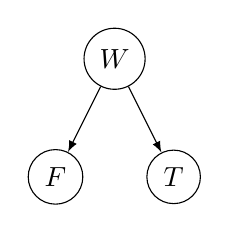
\begin{tikzpicture}[edge from parent/.style={draw,-latex}]
      \node[draw,circle] {$W$}
      child {node[draw,circle] {$F$}}
      child {node[draw,circle] {$T$}};
    \end{tikzpicture}
  \end{subfigure}%
  \begin{subfigure}{0.8\textwidth}
    \centering
    \begin{tabular}[t]{cc}
      \toprule
      $w$ & $\Pr(W = w)$ \\
      \midrule
      1 & 0.5 \\
      0 & 0.5 \\
      \bottomrule
    \end{tabular}
    \begin{tabular}[t]{ccc}
      \toprule
      $w$ & $f$ & $\Pr(F = f \mid W = w)$ \\
      \midrule
      1 & 1 & 0.6 \\
      1 & 0 & 0.4 \\
      0 & 1 & 0.1 \\
      0 & 0 & 0.9 \\
      \bottomrule
    \end{tabular}
    \begin{tabular}[t]{ccc}
      \toprule
      $w$ & $t$ & $\Pr(T = t \mid W = w)$ \\
      \midrule
      1 & $l$ & 0.2 \\
      1 & $m$ & 0.4 \\
      1 & $h$ & 0.4 \\
      0 & $l$ & 0.6 \\
      0 & $m$ & 0.3 \\
      0 & $h$ & 0.1 \\
      \bottomrule
    \end{tabular}
  \end{subfigure}
  \caption{An example Bayesian network with its CPTs}
  \label{fig:example_bn}
\end{figure*}

In this section, we describe a way to encode Bayesian networks into WMC without
restricting oneself to factorable measures and thus having to add extra
variables. We will refer to it as \texttt{cw}.

A Bayesian network is a directed acyclic graph with random variables as vertices
that defines a probability distribution over them. Let $\mathcal{V}$ denote this
set of random variables. For any random variable $X \in \mathcal{V}$, let $\im
X$ denote its set of values and $\mathrm{pa}(X)$ its set of parents. The
full probability distribution is then equal to $\prod_{X \in \mathcal{V}} \Pr(X
\mid \mathrm{pa}(X))$. For discrete Bayesian networks (and we only consider
discrete networks in this paper), each factor of this product can be represented
by a CPT. See \cref{fig:example_bn} for an example Bayesian network that we will
refer to throughout this section. For this network, $\mathcal{V} = \{ W, F, T
\}$, $\mathrm{pa}(W) = \emptyset$, $\mathrm{pa}(F) = \mathrm{pa}(T) = \{ W \}$,
$\im W = \im F = \{0, 1 \}$, and $\im T = \{ l, m, h \}$.

\begin{definition}[Indicator variables]
  Let $X \in \mathcal{V}$ be a random variable. If $X$ is binary (i.e., $|\im X|
  = 2$), we can arbitrary identify one of the values as $1$ and the other one as
  $0$ (i.e, $\im X \cong \{ 0, 1 \}$). Then $X$ can be represented by a single
  \emph{indicator variable} $\lambda_{X=1}$. For notational simplicity, for any
  set $S$, we write $\lambda_{X=0} \in S$ or $S = \{ \lambda_{X=0}, \dots \}$ to
  mean $\lambda_{X=1} \not\in S$.

  On the other hand, if $X$ is not binary, we represent $X$ with $|\im X|$
  indicator variables, one for each value. We let
  \[
    \mathcal{E}(X) = \begin{cases}
      \{ \lambda_{X=1} \} & \text{if } |\im X| = 2 \\
      \{ \lambda_{X=x} \mid x \in \im X \} & \text{otherwise.}
    \end{cases}
  \]
  denote the set of indicator variables for $X$ and $\mathcal{E}^*(X) =
  \mathcal{E}(X) \cup \bigcup_{Y \in \mathrm{pa}(X)} \mathcal{E}(Y)$ denote the
  set of indicator variables for $X$ and its parents in the Bayesian network.
  Finally, let $U = \bigcup_{X \in \mathcal{V}} \mathcal{E}(X)$ denote the set
  of all indicator variables for all random variables in the Bayesian network.
\end{definition}

For example, in the Bayesian network from \cref{fig:example_bn},
$\mathcal{E}^*(T) = \{ \lambda_{T=l}, \lambda_{T=m}, \lambda_{T=h},
\lambda_{W=1} \}$.

\begin{algorithm}[t]
  \KwData{vertices $\mathcal{V}$, probability distribution $\Pr$}
  \KwResult{$\phi\colon 2^U \to \mathbb{R}_{\ge 0}$}
  $\phi \gets 1$\;
  \For{$X \in \mathcal{V}$}{
    \textit{let} $\mathrm{pa}(X) = \{ Y_1, \dots, Y_n \}$\;
    $\mathrm{CPT}_X \gets 0$\;
    \eIf{$|\im X| = 2$}{
      \For{$(y_i)_{i=1}^n \in \prod_{i = 1}^n \im Y_i$}{
        $p_1 \gets \Pr(X = 1 \mid y_1, \dots, y_n)$\;
        $p_0 \gets \Pr(X \ne 1 \mid y_1, \dots, y_n)$\;
        \nosemic $\mathrm{CPT}_X \gets \mathrm{CPT}_X$\;
        \pushline $+ p_1[\lambda_{X=1}] \cdot \prod_{i=1}^n
        [\lambda_{Y_i=y_i}]$\;
        \dosemic $+ p_0 \overline{[\lambda_{X=1}]} \cdot \prod_{i=1}^n
        [\lambda_{Y_i=y_i}]$\;
      }
    }{
      \textit{let} $\im X = \{ x_1, \dots, x_m \}$\;
      \For{$x \in \im X$ {\rm \textbf{and}} $(y_i)_{i=1}^n \in \prod_{i = 1}^n
        \im Y_i$}{
        $p_x \gets \Pr(X = x \mid y_1, \dots, y_n)$\;
        \nosemic $\mathrm{CPT}_X \gets \mathrm{CPT}_X$\;
        \pushline $+ p_x[\lambda_{X=x}] \cdot \prod_{i=1}^n
        [\lambda_{Y_i=y_i}]$\;
        \dosemic $+ \overline{[\lambda_{X=x}]} \cdot \prod_{i=1}^n
        [\lambda_{Y_i=y_i}]$\;
      }
      \nosemic $\mathrm{CPT}_X \gets \mathrm{CPT}_X \cdot \left( \sum_{i=1}^m
        [\lambda_{X = x_i}] \right)$\;
      \pushline\dosemic $\cdot \prod_{i=1}^m \prod_{j=i+1}^m
      (\overline{[\lambda_{X = x_i}]} + \overline{[\lambda_{X = x_j}]})$\;
    }
    $\phi \gets \phi \cdot \mathrm{CPT}_X$\;
  }
  \Return{$\phi$}\;
  \caption{Encoding a Bayesian network}
  \label{alg:encoding}
\end{algorithm}

\Cref{alg:encoding} shows how a Bayesian network with vertices $\mathcal{V}$
can be represented as a weight function $\phi\colon 2^U \to \mathbb{R}_{\ge 0}$.
The algorithm begins with the unit function and multiplies it by
$\mathrm{CPT}_X\colon 2^{\mathcal{E}^*(X)} \to \mathbb{R}_{\ge 0}$ for each
random variable $X \in \mathcal{V}$. We call each such function a
\emph{conditional weight function} as it represents a conditional probability
distribution. However, the distinction is primarily a semantic one: a function
$2^{\{a, b\}} \to \mathbb{R}_{\ge 0}$ can represent $\Pr(a \mid b)$, $\Pr(b \mid
a)$, or something else entirely, e.g., $\Pr(a \land b)$, $\Pr(a \lor b)$, etc.

For a binary random variable $X$, $\mathrm{CPT}_X$ is simply a sum of smaller
functions, one for each row of the CPT. If $X$ has more than two values, we also
multiply $\mathrm{CPT}_X$ by `clause' functions that restrict the value of
$\phi(T)$ to zero whenever $|\mathcal{E}(X) \cap T| \ne 1$. For the Bayesian
network in \cref{fig:example_bn}, we get:
\begin{align*}
  \mathrm{CPT_F} &= 0.6[\lambda_{F=1}] \cdot [\lambda_{W=1}] + 0.4[\lambda_{F=0}] \cdot [\lambda_{W=1}] \\
                 &+ 0.1[\lambda_{F=1}] \cdot [\lambda_{W=0}] + 0.9[\lambda_{F=0}] \cdot [\lambda_{W=0}], \\
  \mathrm{CPT_T} &= ([\lambda_{T=l}] + [\lambda_{T=m}] + [\lambda_{T=h}]) \\
                 &\cdot (\overline{[\lambda_{T=l}]} + \overline{[\lambda_{T=m}]}) \cdot (\overline{[\lambda_{T=l}]} + \overline{[\lambda_{T=h}]}) \\
                 &\cdot (\overline{[\lambda_{T=m}]} + \overline{[\lambda_{T=h}]}) \cdot \dots.
\end{align*}

\subsection{Correctness}

\Cref{alg:encoding} produces a function with a Boolean algebra as its domain.
This function can be represented by an ADD
\cite{DBLP:journals/fmsd/BaharFGHMPS97}. The core of ADDMC works by taking an
ADD $\psi\colon 2^{U} \to \mathbb{R}_{\ge 0}$ (expressed as a product of smaller
ADDs) and returning $(\exists_U\psi)(\emptyset)$
\cite{DBLP:conf/aaai/DudekPV20}. In this section, we prove that the function
$\phi$ produced by \cref{alg:encoding} can be used by ADDMC to correctly compute
any marginal probability of the Bayesian network that was encoded as
$\phi$.\footnote{Note that it can just as well compute \emph{any} probability
  expressed using the random variables in $\mathcal{V}$.} We begin with
\cref{lemma:cpt} which shows that any conditional weight function produces the
right answer when given a valid encoding of variable-value assignments relevant
to the CPT.

\begin{restatable}{lemma}{cptlemma} \label{lemma:cpt}
  Let $X \in \mathcal{V}$ be a random variable with parents $\mathrm{pa}(X) = \{ Y_1,
  \dots, Y_n \}$. Then $\mathrm{CPT}_X\colon 2^{\mathcal{E}^*(X)} \to
  \mathbb{R}_{\ge 0}$ is such that for any $x \in \im X$ and $(y_1, \dots, y_n)
  \in \prod_{i=1}^n \im Y_i$,
  \[
    \mathrm{CPT}_X (T) = \Pr(X = x \mid Y_1 = y_1, \dots, Y_n = y_n),
  \]
  where $T = \{ \lambda_{X=x} \} \cup \{ \lambda_{Y_i=y_i} \mid i = 1, \dots, n
  \}$.
\end{restatable}

Now, \cref{lemma:full_distribution} shows that $\phi$ represents the full
probability distribution of the Bayesian network, i.e., it gives the right
probabilities for the right inputs and zero otherwise. 

\begin{restatable}{lemma}{fulldistribution} \label{lemma:full_distribution}
  Let $\mathcal{V} = \{X_1, \dots, X_n\}$. Then
  \[
    \phi(T) =
    \begin{cases}
      \Pr(x_1, \dots, x_n) &
      \begin{aligned}
        &\text{if } T = \{ \lambda_{X_i=x_i} \}_{i = 1}^n \text{ for} \\
        &\text{some } \textstyle (x_i)_{i=1}^n \in \prod_{i=1}^n \im X_i
      \end{aligned} \\
      0 & \text{otherwise,}
    \end{cases}
  \]
  for all $T \in 2^U$.
\end{restatable}

We end with \cref{thm:correctness} that shows how $\phi$ can be combined with an
encoding of a single variable-value assignment so that ADDMC would compute its
marginal probability.

\begin{restatable}{theorem}{correctness} \label{thm:correctness}
  For any $X \in \mathcal{V}$ and $x \in \im X$,
  \[
    (\exists_U(\phi \cdot [\lambda_{X=x}]))(\emptyset) = \Pr(X = x).
  \]
\end{restatable}

\subsection{Textual Representation} \label{sec:textual_representation}

\Cref{alg:encoding} encodes a Bayesian network into a function on a Boolean
algebra, but how does it relate to the standard interpretation of a WMC encoding
as a formula in conjunctive normal form (CNF) together with a collection of
weights? The factors of $\phi$ that restrict the values of indicator variables
for non-binary random variables are already expressed as a product of sums of
0/1-valued functions, i.e., a kind of CNF. Disregarding these functions, each
conditional weight function $\mathrm{CPT}_X$ is represented by a sum with a term
for every subset of $\mathcal{E}^*(X)$. To encode these terms, we introduce
\emph{extended weight clauses} to the WMC format used by Cachet
\cite{DBLP:conf/sat/SangBBKP04}. For instance, here is a representation of the
Bayesian network from \cref{fig:example_bn}:
\[
  \begin{array}{lrrll}
    \lambda\sb{T=l} &\lambda\sb{T=m} &\lambda\sb{T=h} & &0 \\
                    &-\lambda\sb{T=l} &-\lambda\sb{T=m} & &0 \\
                    &-\lambda\sb{T=l} &-\lambda\sb{T=h} & &0 \\
                    &-\lambda\sb{T=m} &-\lambda\sb{T=h} & &0 \\
    w &\lambda\sb{W=1} & &0.5 &0.5 \\
    w &\lambda\sb{F=1} &\lambda\sb{W=1} &0.6 &0.4 \\
    w &\lambda\sb{F=1} &-\lambda\sb{W=1} &0.1 &0.9 \\
    w &\lambda\sb{T=l} &\lambda\sb{W=1} &0.2 &1 \\
    w &\lambda\sb{T=m} &\lambda\sb{W=1} &0.4 &1 \\
    w &\lambda\sb{T=h} &\lambda\sb{W=1} &0.4 &1 \\
    w &\lambda\sb{T=l} &-\lambda\sb{W=1} &0.6 &1 \\
    w &\lambda\sb{T=m} &-\lambda\sb{W=1} &0.3 &1 \\
    w &\lambda\sb{T=h} &-\lambda\sb{W=1} &0.1 &1
  \end{array}
\]
where each indicator variable is eventually replaced with a unique positive
integer. Each line prefixed with a $w$ can be split into four parts: the `main'
variable (always not negated), conditions (possibly none), and two weights. For
example, the line
\[
  \begin{array}{lrrll}
    w &\lambda\sb{T=m} &-\lambda\sb{W=1} &0.3 &1
  \end{array}
\]
encodes the function $0.3[\lambda_{T=m}] \cdot \overline{[\lambda_{W=1}]} +
1\overline{[\lambda_{T=m}]} \cdot \overline{[\lambda_{W=1}]}$ and can be
interpreted as defining two conditional weights: $\nu(T = m \mid W = 0) = 0.3$,
and $\nu(T \ne m \mid W = 0) = 1$, the former of which corresponds to a row in
the CPT of $T$ while the latter is artificially added as part of the encoding.
In our encoding of Bayesian networks, it is always the case that, in each weight
clause, either both weights sum to one, or the second weight is equal to one.
Finally, note that the measure induced by these weights is not probabilistic
(i.e., $\mu(\top) \ne 1$) by itself, but it becomes probabilistic when combined
with the additional clauses that restrict what combinations of indicator
variables can co-occur.

\subsection{Changes to ADDMC}
% TODO: clarify that both variable orders are handled by the ADDMC heuristics

Here we describe two changes to
ADDMC\footnote{\url{https://github.com/vardigroup/ADDMC}}
\cite{DBLP:conf/aaai/DudekPV20} needed to adapt it to the new format.

% TODO: Gaifman graph is also known as the primal graph
First, ADDMC constructs the \emph{Gaifman graph} of the input CNF formula as an
aid for the algorithm's heuristics. This graph has as vertices the variables of
the formula, and there is an edge between two variables $u$ and $v$ if there is
a clause in the formula that contains both $u$ and $v$. We extend this
definition to functions on Boolean algebras, i.e., the factors of $\phi$. For
any pair of distinct variables $u, v \in U$, we draw an edge between them in the
Gaifman graph if there is a function $\alpha\colon 2^X \to \mathbb{R}_{\ge 0}$
that is a factor of $\phi$ such that $u \in X$ and $v \in X$. For instance, a
factor such as $\mathrm{CPT}_X$ will enable edges between all distinct pairs of
variables in $\mathcal{E}^*(X)$.

Second, even though the function $\phi$ produced by \cref{alg:encoding} is
constructed to have $2^U$ as its domain, sometimes the domain is effectively
reduced to $2^V$ for some $V \subset U$ by the ADD manipulation algorithms that
optimise the ADD representation of a function. For a simple example, consider
$\alpha: 2^{\{a\}} \to \mathbb{R}_{\ge 0}$ defined as $\alpha(\{a\}) =
\alpha(\emptyset) = 0.5$. Then $\alpha$ can be reduced to $\alpha'\colon
2^{\emptyset} \to \mathbb{R}_{\ge 0}$ defined as $\alpha'(\emptyset) = 0.5$. To
compensate for these reductions, for the original WMC format with a weight
function $w\colon U \cup \{ \neg u \mid u \in U \} \to \mathbb{R}_{\ge 0}$,
ADDMC would multiply its computed answer by $\prod_{u \in U \setminus V} w(u) +
w(\neg u)$. With the new WMC format, we instead multiply the answer by $2^{|U
  \setminus V|}$. Each `excluded' variable $u \in U \setminus V$ satisfies two
properties: all weights associated with $u$ are equal to $0.5$ (otherwise the
corresponding CPT would depend on $u$, and $u$ would not be excluded), and all
other CPTs are independent of $u$ (or they may have a trivial dependence, where
the probability stays the same if $u$ is replaced with its complement). Thus,
the CPT that corresponds to $u$ still multiplies the weight of every atom in the
Boolean algebra by $0.5$, but the number of atoms under consideration is halved.
To correct for this, we multiply the final answer by two for every $u \in U
\setminus V$.

\section{Experimental Comparison} \label{sec:experiments}
% TODO: stacked bar charts: 1) mention that the error bars denote 0.1 * standard
% deviation
% 2) and that only successfully run instances are included
% 3) and that the top error bar relates only to inference (and not the sum of
% the two)
% TODO: note: I'm unable to replicate the experiments from bklm. This could be
% due to two reasons:
% 1) I'm measuring running time rather than compiled structure size <- more
% likely
% 2) I'm not using the -implicit flag.
% TODO: We use Ace to compile the BN together with its evidence (as opposed to
% compiling just the BN and using evidence during inference) as this more
% closely resembles the behaviour of ADDMC
% TODO: we run cd05 only with dtBnMinfill, as that's the more commonly used
% setting (although another one was used as well)
% TODO: The -implicit flag of bklm16 cannot be used because even a small
% Bayesian network with seven independent binary variables with 0.1/0.9
% probabilities is already big enough to drive the scaling factor down to zero.
% The last step of this encoding is a multiplication of a huge number (on the
% order of 10^30 for some of the smaller DQMR instances) by a number
% equivalently close to zero (so that their product lands in the interval [0,
% 1]). Thus, we disable this flag (thus making the algorithm slower but
% correct).
% TODO: the legacy mode encoding of bklm16 also runs c2d (as packaged with Ace)
% TODO: Note that our encoder was implemented in Python with no concern for
% efficiency, so encoding could easily be improved by one or two orders of
% magnitude.
% TODO: Python, Java, gcc versions (maybe also all the software that I'm using
% (e.g., bn2cnf, Cachet))
% TODO: 85% is as recommended in the README of Ace (might have to go lower than that)
% TODO: for each encoding, mention:
% 1) software
% 2) encoding options
% 3) additional data processing
% 4) inference options

TODO: Things I will need to mention:
\begin{itemize}
\item
  \texttt{query-dnnf}\footnote{\url{http://www.cril.univ-artois.fr/kc/d-DNNF-reasoner.html}}
\item
  \texttt{bn2cnf}\footnote{\url{http://www.cril.univ-artois.fr/KC/bn2cnf.html}}
  and \texttt{bklm16} \cite{DBLP:conf/ecai/BartKLM16}
\end{itemize}

In this section, we describe an experimental study comparing the five WMC
encodings for Bayesian networks when run with ADDMC. The experiments were run on
servers with Intel Xeon Gold 6138 and Intel Xeon E5-2630
processors\footnote{Each instance is run on the same processor for all
  encodings.} running Scientific~Linux~7 with an \SI{8}{\gibi\byte} memory limit
and a \SI{1000}{\second} timeout.

For each Bayesian network, we need to choose a probability to compute. Whenever
a Bayesian network comes with an evidence file, we compute the probability of
evidence. Otherwise, let $X$ denote the last-mentioned vertex in the Bayesian
network. If $\mathsf{true} \in \im X$, then we compute the marginal probability
of $X = \mathsf{true}$. Otherwise, we pick the value of $X$ which is listed
first and calculate its marginal probability.

For all encodings other than \texttt{cw}, we use their implementation in
Ace~3.0\footnote{\url{http://reasoning.cs.ucla.edu/ace/}} with
\texttt{-encodeOnly} and \texttt{-noEclause} flags. However, Ace was not used to
encode evidence, as preliminary experiments revealed that the evidence-encoding
implementation contains bugs that can lead to incorrect answers or a Java
exception being thrown on some instances of the data set (and the source code is
not publicly available). Instead, we simply list all the evidence as additional
clauses in the encoding.

Note that both \texttt{cd05} and \texttt{cd06} purposefully produce overly
relaxed encodings that contain extra models and thus yield incorrect
probabilities \cite{DBLP:conf/ijcai/ChaviraD05,DBLP:conf/sat/ChaviraD06}. These
additional models are supposed to be filtered out during circuit compilation
\cite{DBLP:conf/ijcai/ChaviraD05}, but this is not easily achievable with ADDMC.
Nonetheless, we include both encodings in the experiments.

While encoding time itself was not measured because of different languages of
implementation, it is worth noting that \texttt{cw} is linear in the total
number of CPT rows and so is unlikely to be slower than, e.g., \texttt{cd06},
which relies on solving $\NP{}$-complete problems as part of the encoding process
\cite{DBLP:conf/sat/ChaviraD06}.

For experimental data, we use the Bayesian networks available with Ace and
Cachet\footnote{\url{https://www.cs.rochester.edu/u/kautz/Cachet/}}, most of
which happen to be binary. We classify them into the following seven categories:
\begin{itemize*}
\item DQMR and
\item Grid networks as described by Sang
  \etal{}~\shortcite{DBLP:conf/aaai/SangBK05},
\item Mastermind, and
\item Random Blocks from the work of Chavira
  \etal{}~\shortcite{DBLP:journals/ijar/ChaviraDJ06},
\item remaining binary Bayesian networks that include Plan Recognition
  \cite{DBLP:conf/aaai/SangBK05}, Friends and Smokers, Students and Professors
  \cite{DBLP:journals/ijar/ChaviraDJ06}, and \texttt{tcc4f}, and
\item non-binary classic Bayesian networks (\texttt{alarm}, \texttt{diabetes},
  \texttt{hailfinder}, \texttt{mildew}, \texttt{munin1}--\texttt{4},
  \texttt{pathfinder}, \texttt{pigs}, \texttt{water}).
\end{itemize*}
We run ADDMC with each of the five encodings once on each Bayesian network.

\begin{figure}
  \centering
  % Created by tikzDevice version 0.12.3 on 2020-08-17 17:59:12
% !TEX encoding = UTF-8 Unicode
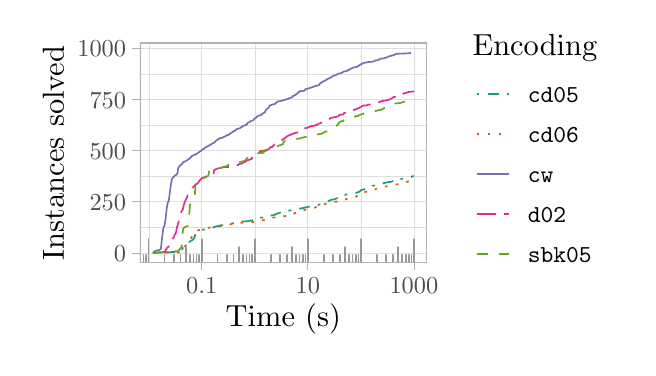
\begin{tikzpicture}[x=1pt,y=1pt]
\definecolor{fillColor}{RGB}{255,255,255}
\path[use as bounding box,fill=fillColor,fill opacity=0.00] (0,0) rectangle (216.81,115.63);
\begin{scope}
\path[clip] (  0.00,  0.00) rectangle (216.81,115.63);
\definecolor{drawColor}{RGB}{255,255,255}
\definecolor{fillColor}{RGB}{255,255,255}

\path[draw=drawColor,line width= 0.6pt,line join=round,line cap=round,fill=fillColor] (  0.00,  0.00) rectangle (216.81,115.63);
\end{scope}
\begin{scope}
\path[clip] ( 40.51, 30.69) rectangle (144.25,110.13);
\definecolor{fillColor}{RGB}{255,255,255}

\path[fill=fillColor] ( 40.51, 30.69) rectangle (144.25,110.13);
\definecolor{drawColor}{gray}{0.87}

\path[draw=drawColor,line width= 0.1pt,line join=round] ( 40.51, 43.45) --
	(144.25, 43.45);

\path[draw=drawColor,line width= 0.1pt,line join=round] ( 40.51, 61.92) --
	(144.25, 61.92);

\path[draw=drawColor,line width= 0.1pt,line join=round] ( 40.51, 80.38) --
	(144.25, 80.38);

\path[draw=drawColor,line width= 0.1pt,line join=round] ( 40.51, 98.84) --
	(144.25, 98.84);

\path[draw=drawColor,line width= 0.1pt,line join=round] ( 43.71, 30.69) --
	( 43.71,110.13);

\path[draw=drawColor,line width= 0.1pt,line join=round] ( 82.05, 30.69) --
	( 82.05,110.13);

\path[draw=drawColor,line width= 0.1pt,line join=round] (120.40, 30.69) --
	(120.40,110.13);

\path[draw=drawColor,line width= 0.3pt,line join=round] ( 40.51, 34.22) --
	(144.25, 34.22);

\path[draw=drawColor,line width= 0.3pt,line join=round] ( 40.51, 52.69) --
	(144.25, 52.69);

\path[draw=drawColor,line width= 0.3pt,line join=round] ( 40.51, 71.15) --
	(144.25, 71.15);

\path[draw=drawColor,line width= 0.3pt,line join=round] ( 40.51, 89.61) --
	(144.25, 89.61);

\path[draw=drawColor,line width= 0.3pt,line join=round] ( 40.51,108.07) --
	(144.25,108.07);

\path[draw=drawColor,line width= 0.3pt,line join=round] ( 62.88, 30.69) --
	( 62.88,110.13);

\path[draw=drawColor,line width= 0.3pt,line join=round] (101.22, 30.69) --
	(101.22,110.13);

\path[draw=drawColor,line width= 0.3pt,line join=round] (139.57, 30.69) --
	(139.57,110.13);
\definecolor{drawColor}{RGB}{27,158,119}

\path[draw=drawColor,line width= 0.6pt,dash pattern=on 1pt off 3pt on 4pt off 3pt ,line join=round] ( 45.23, 34.30) --
	( 55.46, 34.67) --
	( 55.66, 35.11) --
	( 55.85, 35.63) --
	( 56.04, 36.00) --
	( 56.23, 36.22) --
	( 56.41, 36.36) --
	( 57.44, 36.59) --
	( 57.90, 36.81) --
	( 58.05, 37.25) --
	( 58.20, 37.55) --
	( 58.34, 37.99) --
	( 58.49, 38.21) --
	( 58.63, 38.36) --
	( 58.76, 38.43) --
	( 58.90, 38.51) --
	( 59.03, 38.58) --
	( 59.29, 38.73) --
	( 59.42, 38.80) --
	( 59.55, 38.88) --
	( 59.67, 39.02) --
	( 59.91, 39.17) --
	( 60.03, 39.47) --
	( 60.14, 39.61) --
	( 60.26, 39.84) --
	( 60.37, 40.20) --
	( 60.48, 40.65) --
	( 60.59, 40.80) --
	( 60.70, 40.87) --
	( 60.81, 41.16) --
	( 60.92, 41.24) --
	( 61.02, 41.39) --
	( 61.13, 41.46) --
	( 61.43, 41.61) --
	( 61.82, 41.68) --
	( 61.91, 41.76) --
	( 62.00, 41.83) --
	( 62.09, 41.90) --
	( 62.19, 42.12) --
	( 62.28, 42.20) --
	( 62.36, 42.35) --
	( 62.45, 42.42) --
	( 62.63, 42.49) --
	( 62.96, 42.57) --
	( 63.21, 42.64) --
	( 63.90, 42.72) --
	( 63.97, 42.79) --
	( 64.12, 42.94) --
	( 64.67, 43.01) --
	( 64.74, 43.08) --
	( 65.06, 43.16) --
	( 65.44, 43.23) --
	( 65.56, 43.31) --
	( 66.74, 43.38) --
	( 67.20, 43.45) --
	( 67.30, 43.53) --
	( 67.35, 43.60) --
	( 67.49, 43.68) --
	( 67.77, 43.75) --
	( 68.35, 43.82) --
	( 68.48, 43.90) --
	( 68.82, 43.97) --
	( 69.18, 44.04) --
	( 69.33, 44.12) --
	( 69.63, 44.19) --
	( 70.61, 44.27) --
	( 71.24, 44.34) --
	( 71.27, 44.41) --
	( 71.60, 44.49) --
	( 71.97, 44.56) --
	( 72.90, 44.64) --
	( 73.07, 44.71) --
	( 73.29, 44.78) --
	( 73.75, 44.86) --
	( 74.15, 44.93) --
	( 74.71, 45.01) --
	( 75.31, 45.08) --
	( 75.57, 45.15) --
	( 75.66, 45.23) --
	( 75.69, 45.30) --
	( 75.91, 45.37) --
	( 77.01, 45.45) --
	( 77.31, 45.52) --
	( 77.46, 45.60) --
	( 79.12, 45.67) --
	( 79.78, 45.74) --
	( 80.13, 45.82) --
	( 80.29, 45.89) --
	( 80.61, 45.97) --
	( 81.66, 46.04) --
	( 81.70, 46.11) --
	( 81.95, 46.19) --
	( 82.89, 46.26) --
	( 82.96, 46.33) --
	( 82.97, 46.41) --
	( 83.43, 46.48) --
	( 83.49, 46.56) --
	( 83.52, 46.63) --
	( 83.96, 46.78) --
	( 84.09, 46.85) --
	( 84.34, 46.93) --
	( 84.67, 47.00) --
	( 85.31, 47.07) --
	( 85.45, 47.15) --
	( 85.57, 47.22) --
	( 85.75, 47.29) --
	( 85.81, 47.37) --
	( 85.82, 47.44) --
	( 85.83, 47.52) --
	( 85.86, 47.59) --
	( 85.97, 47.66) --
	( 88.13, 47.74) --
	( 88.44, 47.81) --
	( 88.92, 47.89) --
	( 89.04, 47.96) --
	( 89.11, 48.03) --
	( 89.54, 48.11) --
	( 89.67, 48.18) --
	( 89.70, 48.25) --
	( 89.77, 48.33) --
	( 90.10, 48.40) --
	( 90.23, 48.48) --
	( 90.36, 48.55) --
	( 90.67, 48.62) --
	( 90.95, 48.70) --
	( 91.16, 48.77) --
	( 91.51, 48.85) --
	( 91.53, 48.92) --
	( 91.56, 48.99) --
	( 91.60, 49.07) --
	( 91.86, 49.14) --
	( 92.40, 49.21) --
	( 93.74, 49.29) --
	( 94.31, 49.36) --
	( 94.38, 49.44) --
	( 94.53, 49.51) --
	( 94.63, 49.58) --
	( 95.59, 49.66) --
	( 95.79, 49.73) --
	( 96.97, 49.81) --
	( 97.20, 49.88) --
	( 97.28, 49.95) --
	( 97.34, 50.03) --
	( 97.60, 50.10) --
	( 98.53, 50.17) --
	( 98.58, 50.25) --
	( 98.80, 50.32) --
	( 98.89, 50.40) --
	( 99.54, 50.47) --
	( 99.87, 50.54) --
	( 99.99, 50.62) --
	(100.88, 50.69) --
	(100.90, 50.77) --
	(101.23, 50.84) --
	(101.59, 50.91) --
	(101.78, 50.99) --
	(101.94, 51.06) --
	(102.34, 51.13) --
	(102.60, 51.21) --
	(103.47, 51.28) --
	(104.09, 51.36) --
	(104.22, 51.43) --
	(104.79, 51.50) --
	(105.03, 51.58) --
	(105.09, 51.65) --
	(105.18, 51.73) --
	(106.21, 51.80) --
	(106.26, 51.87) --
	(106.42, 51.95) --
	(106.83, 52.02) --
	(106.96, 52.09) --
	(106.97, 52.17) --
	(107.04, 52.24) --
	(107.10, 52.32) --
	(107.23, 52.39) --
	(107.24, 52.46) --
	(107.33, 52.54) --
	(107.50, 52.61) --
	(107.64, 52.69) --
	(107.92, 52.76) --
	(108.08, 52.83) --
	(108.71, 52.91) --
	(108.84, 52.98) --
	(108.85, 53.05) --
	(109.01, 53.13) --
	(109.31, 53.20) --
	(109.34, 53.28) --
	(109.36, 53.35) --
	(109.64, 53.42) --
	(110.28, 53.50) --
	(110.74, 53.57) --
	(110.80, 53.65) --
	(111.20, 53.72) --
	(111.31, 53.79) --
	(111.44, 53.87) --
	(111.61, 53.94) --
	(111.67, 54.01) --
	(112.07, 54.09) --
	(113.19, 54.16) --
	(113.33, 54.24) --
	(113.37, 54.31) --
	(113.40, 54.38) --
	(113.43, 54.46) --
	(113.55, 54.53) --
	(113.59, 54.61) --
	(113.60, 54.68) --
	(113.92, 54.75) --
	(113.94, 54.83) --
	(114.01, 54.90) --
	(114.16, 54.97) --
	(114.18, 55.05) --
	(114.24, 55.12) --
	(114.73, 55.20) --
	(114.89, 55.27) --
	(115.26, 55.34) --
	(116.17, 55.42) --
	(116.30, 55.49) --
	(116.65, 55.57) --
	(116.76, 55.64) --
	(117.14, 55.71) --
	(117.52, 55.79) --
	(118.08, 55.86) --
	(118.43, 55.93) --
	(118.99, 56.01) --
	(119.08, 56.08) --
	(119.22, 56.16) --
	(119.58, 56.23) --
	(119.82, 56.30) --
	(119.94, 56.38) --
	(119.96, 56.45) --
	(119.97, 56.53) --
	(120.20, 56.60) --
	(120.24, 56.67) --
	(120.28, 56.75) --
	(120.32, 56.82) --
	(120.33, 56.89) --
	(120.75, 56.97) --
	(120.93, 57.04) --
	(121.35, 57.12) --
	(121.55, 57.19) --
	(121.70, 57.26) --
	(121.96, 57.34) --
	(122.25, 57.41) --
	(122.25, 57.49) --
	(122.31, 57.56) --
	(122.42, 57.63) --
	(122.52, 57.71) --
	(122.63, 57.78) --
	(122.88, 57.85) --
	(122.94, 57.93) --
	(123.13, 58.00) --
	(123.42, 58.08) --
	(123.72, 58.15) --
	(123.83, 58.22) --
	(123.98, 58.30) --
	(124.05, 58.37) --
	(124.62, 58.45) --
	(124.63, 58.52) --
	(125.67, 58.59) --
	(126.16, 58.67) --
	(126.57, 58.74) --
	(126.76, 58.81) --
	(126.78, 58.89) --
	(126.79, 58.96) --
	(127.13, 59.04) --
	(127.14, 59.11) --
	(127.45, 59.18) --
	(127.81, 59.26) --
	(128.20, 59.33) --
	(128.56, 59.41) --
	(128.63, 59.48) --
	(129.26, 59.55) --
	(129.31, 59.63) --
	(129.35, 59.70) --
	(130.36, 59.77) --
	(130.40, 59.85) --
	(131.29, 59.92) --
	(131.50, 60.00) --
	(131.61, 60.07) --
	(131.80, 60.14) --
	(131.82, 60.22) --
	(132.24, 60.29) --
	(132.31, 60.37) --
	(132.38, 60.44) --
	(133.06, 60.51) --
	(133.08, 60.59) --
	(133.09, 60.66) --
	(133.74, 60.73) --
	(133.80, 60.81) --
	(133.81, 60.88) --
	(133.89, 60.96) --
	(136.18, 61.03) --
	(136.63, 61.10) --
	(136.69, 61.18) --
	(136.75, 61.25) --
	(137.05, 61.33) --
	(137.21, 61.40) --
	(137.44, 61.47) --
	(138.04, 61.55) --
	(138.28, 61.62) --
	(138.65, 61.69) --
	(138.77, 61.77) --
	(138.91, 61.84) --
	(139.02, 61.92) --
	(139.20, 61.99) --
	(139.49, 62.06);
\definecolor{drawColor}{RGB}{217,95,2}

\path[draw=drawColor,line width= 0.6pt,dash pattern=on 1pt off 3pt ,line join=round] ( 45.89, 34.30) --
	( 54.60, 34.37) --
	( 54.82, 34.67) --
	( 55.04, 35.55) --
	( 55.25, 36.00) --
	( 55.46, 36.29) --
	( 55.85, 36.44) --
	( 56.41, 36.51) --
	( 56.59, 36.66) --
	( 56.94, 36.73) --
	( 57.11, 36.81) --
	( 57.27, 37.40) --
	( 57.44, 37.92) --
	( 57.59, 38.21) --
	( 57.75, 38.51) --
	( 58.05, 38.73) --
	( 58.20, 38.80) --
	( 58.34, 39.02) --
	( 58.76, 39.17) --
	( 58.90, 39.24) --
	( 59.03, 39.47) --
	( 59.16, 39.69) --
	( 59.29, 40.13) --
	( 59.42, 40.57) --
	( 59.55, 40.87) --
	( 59.67, 41.09) --
	( 59.79, 41.24) --
	( 59.91, 41.53) --
	( 60.03, 41.61) --
	( 60.14, 41.68) --
	( 60.26, 41.76) --
	( 60.48, 41.83) --
	( 60.59, 41.90) --
	( 60.81, 41.98) --
	( 60.92, 42.12) --
	( 61.23, 42.20) --
	( 61.33, 42.27) --
	( 61.53, 42.35) --
	( 61.72, 42.42) --
	( 61.91, 42.49) --
	( 62.36, 42.57) --
	( 62.80, 42.64) --
	( 62.88, 42.72) --
	( 63.60, 42.79) --
	( 63.90, 42.86) --
	( 64.12, 42.94) --
	( 64.40, 43.08) --
	( 64.74, 43.16) --
	( 64.80, 43.23) --
	( 65.13, 43.31) --
	( 65.80, 43.38) --
	( 67.40, 43.45) --
	( 67.77, 43.53) --
	( 68.48, 43.60) --
	( 68.53, 43.68) --
	( 68.57, 43.75) --
	( 69.29, 43.82) --
	( 69.52, 43.90) --
	( 70.64, 43.97) --
	( 71.21, 44.04) --
	( 71.63, 44.12) --
	( 71.80, 44.19) --
	( 72.19, 44.27) --
	( 72.33, 44.34) --
	( 72.56, 44.41) --
	( 72.80, 44.49) --
	( 73.17, 44.56) --
	( 74.32, 44.71) --
	( 74.46, 44.78) --
	( 74.89, 44.86) --
	( 75.62, 44.93) --
	( 76.26, 45.01) --
	( 76.89, 45.08) --
	( 77.64, 45.15) --
	( 77.69, 45.23) --
	( 80.18, 45.30) --
	( 80.84, 45.37) --
	( 82.18, 45.45) --
	( 82.44, 45.52) --
	( 83.05, 45.60) --
	( 83.30, 45.67) --
	( 83.98, 45.74) --
	( 84.55, 45.82) --
	( 84.56, 45.89) --
	( 84.58, 45.97) --
	( 84.70, 46.04) --
	( 85.27, 46.11) --
	( 85.80, 46.19) --
	( 86.34, 46.26) --
	( 86.47, 46.33) --
	( 87.34, 46.41) --
	( 87.39, 46.48) --
	( 87.68, 46.56) --
	( 87.82, 46.63) --
	( 88.03, 46.70) --
	( 88.21, 46.78) --
	( 88.45, 46.85) --
	( 88.55, 46.93) --
	( 88.69, 47.00) --
	( 89.51, 47.07) --
	( 90.37, 47.15) --
	( 90.43, 47.22) --
	( 90.45, 47.29) --
	( 90.72, 47.37) --
	( 92.22, 47.44) --
	( 92.67, 47.52) --
	( 93.62, 47.59) --
	( 93.82, 47.66) --
	( 94.09, 47.74) --
	( 94.12, 47.81) --
	( 94.21, 47.89) --
	( 94.21, 47.96) --
	( 94.23, 48.03) --
	( 94.26, 48.11) --
	( 94.54, 48.18) --
	( 95.37, 48.25) --
	( 95.84, 48.33) --
	( 96.29, 48.40) --
	( 96.33, 48.48) --
	( 96.35, 48.55) --
	( 96.62, 48.62) --
	( 97.01, 48.70) --
	( 97.28, 48.77) --
	( 97.74, 48.85) --
	( 97.98, 48.92) --
	( 98.28, 48.99) --
	( 98.48, 49.07) --
	( 98.57, 49.14) --
	( 98.76, 49.21) --
	( 98.78, 49.29) --
	( 98.94, 49.36) --
	( 99.02, 49.44) --
	( 99.29, 49.51) --
	( 99.47, 49.58) --
	( 99.59, 49.66) --
	( 99.73, 49.73) --
	(100.33, 49.81) --
	(100.42, 49.88) --
	(101.26, 49.95) --
	(101.37, 50.03) --
	(101.43, 50.10) --
	(101.58, 50.17) --
	(101.79, 50.25) --
	(102.10, 50.32) --
	(102.30, 50.40) --
	(103.19, 50.47) --
	(103.48, 50.54) --
	(103.94, 50.62) --
	(103.94, 50.69) --
	(104.06, 50.77) --
	(104.25, 50.84) --
	(104.36, 50.91) --
	(104.51, 50.99) --
	(104.87, 51.06) --
	(104.87, 51.13) --
	(105.20, 51.21) --
	(105.47, 51.28) --
	(105.59, 51.36) --
	(105.63, 51.43) --
	(106.09, 51.50) --
	(106.19, 51.58) --
	(106.20, 51.65) --
	(106.31, 51.73) --
	(106.32, 51.80) --
	(106.47, 51.87) --
	(107.77, 51.95) --
	(107.84, 52.02) --
	(108.52, 52.09) --
	(108.89, 52.17) --
	(109.25, 52.24) --
	(109.44, 52.32) --
	(109.91, 52.39) --
	(110.27, 52.46) --
	(110.38, 52.54) --
	(110.74, 52.61) --
	(110.90, 52.69) --
	(111.50, 52.76) --
	(111.69, 52.83) --
	(111.73, 52.91) --
	(111.77, 52.98) --
	(111.78, 53.05) --
	(111.92, 53.13) --
	(112.69, 53.20) --
	(113.17, 53.28) --
	(113.81, 53.35) --
	(114.28, 53.42) --
	(114.59, 53.50) --
	(114.88, 53.57) --
	(114.89, 53.65) --
	(115.08, 53.72) --
	(115.35, 53.79) --
	(115.69, 53.87) --
	(115.87, 53.94) --
	(116.52, 54.01) --
	(117.14, 54.09) --
	(117.45, 54.16) --
	(117.45, 54.24) --
	(117.47, 54.31) --
	(117.66, 54.38) --
	(118.16, 54.46) --
	(118.33, 54.53) --
	(118.82, 54.61) --
	(118.95, 54.68) --
	(119.00, 54.75) --
	(119.01, 54.83) --
	(119.02, 54.90) --
	(119.06, 54.97) --
	(119.12, 55.05) --
	(119.12, 55.12) --
	(119.12, 55.20) --
	(119.35, 55.27) --
	(119.44, 55.34) --
	(119.55, 55.42) --
	(119.67, 55.49) --
	(120.23, 55.57) --
	(120.43, 55.64) --
	(120.81, 55.71) --
	(120.85, 55.79) --
	(120.92, 55.86) --
	(120.97, 55.93) --
	(121.01, 56.01) --
	(121.08, 56.08) --
	(121.55, 56.16) --
	(121.92, 56.23) --
	(122.05, 56.30) --
	(122.30, 56.38) --
	(122.51, 56.45) --
	(122.57, 56.53) --
	(122.59, 56.60) --
	(122.74, 56.67) --
	(123.04, 56.75) --
	(123.22, 56.82) --
	(123.79, 56.89) --
	(123.79, 56.97) --
	(124.39, 57.04) --
	(124.54, 57.12) --
	(125.56, 57.19) --
	(125.79, 57.26) --
	(125.80, 57.34) --
	(125.94, 57.41) --
	(126.49, 57.49) --
	(126.52, 57.56) --
	(126.76, 57.63) --
	(127.26, 57.71) --
	(127.41, 57.78) --
	(127.46, 57.85) --
	(128.00, 57.93) --
	(128.06, 58.00) --
	(128.15, 58.08) --
	(128.32, 58.15) --
	(128.61, 58.22) --
	(130.12, 58.30) --
	(130.53, 58.37) --
	(131.04, 58.45) --
	(131.30, 58.52) --
	(131.46, 58.59) --
	(131.67, 58.67) --
	(132.11, 58.74) --
	(132.56, 58.81) --
	(132.75, 58.89) --
	(132.94, 58.96) --
	(133.58, 59.04) --
	(134.45, 59.11) --
	(135.06, 59.18) --
	(135.14, 59.26) --
	(135.26, 59.33) --
	(135.36, 59.41) --
	(136.06, 59.48) --
	(136.11, 59.55) --
	(136.26, 59.63) --
	(136.32, 59.70) --
	(136.67, 59.77) --
	(136.85, 59.85) --
	(137.14, 59.92) --
	(137.42, 60.00) --
	(137.53, 60.07) --
	(137.58, 60.14) --
	(137.68, 60.22) --
	(137.86, 60.29) --
	(138.15, 60.37) --
	(138.17, 60.44) --
	(138.27, 60.51) --
	(138.48, 60.59) --
	(138.51, 60.66) --
	(138.75, 60.73);
\definecolor{drawColor}{RGB}{117,112,179}

\path[draw=drawColor,line width= 0.6pt,line join=round] ( 45.23, 34.30) --
	( 45.89, 34.81) --
	( 46.51, 35.11) --
	( 47.08, 35.18) --
	( 47.62, 35.33) --
	( 48.13, 35.70) --
	( 48.60, 39.84) --
	( 49.05, 43.38) --
	( 49.48, 44.19) --
	( 49.89, 46.93) --
	( 50.27, 50.62) --
	( 50.64, 52.46) --
	( 51.00, 53.13) --
	( 51.34, 55.86) --
	( 51.66, 58.22) --
	( 51.98, 60.37) --
	( 52.28, 61.18) --
	( 52.57, 61.62) --
	( 52.86, 61.77) --
	( 53.13, 62.14) --
	( 53.65, 62.43) --
	( 53.90, 62.65) --
	( 54.14, 63.10) --
	( 54.37, 64.72) --
	( 54.60, 65.24) --
	( 54.82, 65.53) --
	( 55.04, 65.83) --
	( 55.25, 65.98) --
	( 55.66, 66.20) --
	( 55.85, 66.57) --
	( 56.04, 66.86) --
	( 56.23, 67.01) --
	( 56.41, 67.16) --
	( 56.77, 67.23) --
	( 56.94, 67.31) --
	( 57.11, 67.45) --
	( 57.27, 67.60) --
	( 57.59, 67.75) --
	( 57.75, 67.82) --
	( 57.90, 67.90) --
	( 58.05, 68.12) --
	( 58.34, 68.19) --
	( 58.49, 68.34) --
	( 58.63, 68.56) --
	( 58.76, 68.64) --
	( 58.90, 68.78) --
	( 59.03, 68.86) --
	( 59.16, 69.08) --
	( 59.29, 69.23) --
	( 59.55, 69.30) --
	( 59.67, 69.38) --
	( 59.79, 69.45) --
	( 60.14, 69.67) --
	( 60.59, 69.74) --
	( 60.70, 69.89) --
	( 60.92, 69.97) --
	( 61.02, 70.04) --
	( 61.23, 70.11) --
	( 61.43, 70.26) --
	( 61.62, 70.41) --
	( 61.72, 70.48) --
	( 61.82, 70.56) --
	( 61.91, 70.63) --
	( 62.00, 70.70) --
	( 62.09, 70.78) --
	( 62.19, 70.85) --
	( 62.45, 71.00) --
	( 62.63, 71.07) --
	( 62.71, 71.15) --
	( 62.80, 71.30) --
	( 62.96, 71.52) --
	( 63.13, 71.59) --
	( 63.29, 71.74) --
	( 63.67, 71.81) --
	( 63.75, 71.89) --
	( 63.82, 71.96) --
	( 63.90, 72.03) --
	( 64.04, 72.18) --
	( 64.19, 72.26) --
	( 64.26, 72.40) --
	( 64.54, 72.48) --
	( 64.67, 72.55) --
	( 64.87, 72.62) --
	( 64.94, 72.70) --
	( 65.06, 72.77) --
	( 65.19, 72.85) --
	( 65.32, 72.92) --
	( 65.38, 73.07) --
	( 65.86, 73.14) --
	( 65.97, 73.22) --
	( 66.09, 73.36) --
	( 66.14, 73.44) --
	( 66.26, 73.51) --
	( 66.53, 73.58) --
	( 66.58, 73.73) --
	( 66.79, 73.81) --
	( 67.00, 73.88) --
	( 67.05, 73.95) --
	( 67.30, 74.03) --
	( 67.49, 74.10) --
	( 67.54, 74.18) --
	( 67.68, 74.32) --
	( 67.73, 74.40) --
	( 67.77, 74.47) --
	( 67.82, 74.54) --
	( 67.91, 74.62) --
	( 67.96, 74.69) --
	( 68.05, 74.77) --
	( 68.14, 74.84) --
	( 68.18, 74.91) --
	( 68.40, 74.99) --
	( 68.57, 75.06) --
	( 68.69, 75.21) --
	( 68.98, 75.28) --
	( 69.02, 75.50) --
	( 69.21, 75.58) --
	( 69.44, 75.65) --
	( 69.52, 75.73) --
	( 70.10, 75.80) --
	( 70.38, 75.87) --
	( 70.61, 75.95) --
	( 70.64, 76.02) --
	( 70.71, 76.10) --
	( 70.99, 76.17) --
	( 71.06, 76.24) --
	( 71.24, 76.32) --
	( 71.36, 76.39) --
	( 71.57, 76.46) --
	( 71.63, 76.54) --
	( 71.80, 76.61) --
	( 71.92, 76.69) --
	( 72.06, 76.76) --
	( 72.17, 76.83) --
	( 72.49, 76.91) --
	( 72.59, 76.98) --
	( 72.87, 77.06) --
	( 72.97, 77.13) --
	( 73.09, 77.20) --
	( 73.17, 77.28) --
	( 73.19, 77.35) --
	( 73.24, 77.42) --
	( 73.31, 77.50) --
	( 73.38, 77.57) --
	( 73.52, 77.65) --
	( 73.68, 77.72) --
	( 74.00, 77.87) --
	( 74.10, 77.94) --
	( 74.19, 78.02) --
	( 74.28, 78.16) --
	( 74.42, 78.24) --
	( 74.87, 78.31) --
	( 74.93, 78.38) --
	( 74.97, 78.46) --
	( 75.08, 78.61) --
	( 75.16, 78.68) --
	( 75.20, 78.75) --
	( 75.31, 78.90) --
	( 75.59, 78.98) --
	( 75.62, 79.05) --
	( 76.13, 79.12) --
	( 76.36, 79.20) --
	( 76.72, 79.27) --
	( 76.73, 79.34) --
	( 76.80, 79.42) --
	( 77.01, 79.49) --
	( 77.07, 79.57) --
	( 77.10, 79.64) --
	( 77.22, 79.71) --
	( 77.49, 79.79) --
	( 77.52, 79.86) --
	( 77.73, 80.01) --
	( 77.88, 80.08) --
	( 78.05, 80.16) --
	( 78.15, 80.23) --
	( 78.39, 80.30) --
	( 78.49, 80.38) --
	( 78.66, 80.45) --
	( 79.09, 80.53) --
	( 79.17, 80.60) --
	( 79.22, 80.75) --
	( 79.26, 80.82) --
	( 79.33, 80.97) --
	( 79.42, 81.04) --
	( 79.44, 81.12) --
	( 79.53, 81.19) --
	( 79.55, 81.26) --
	( 79.60, 81.34) --
	( 79.93, 81.41) --
	( 80.02, 81.49) --
	( 80.20, 81.56) --
	( 80.33, 81.63) --
	( 80.39, 81.71) --
	( 80.46, 81.78) --
	( 80.58, 81.86) --
	( 80.69, 81.93) --
	( 80.81, 82.00) --
	( 81.31, 82.08) --
	( 81.53, 82.15) --
	( 81.59, 82.22) --
	( 81.61, 82.30) --
	( 81.68, 82.37) --
	( 81.73, 82.45) --
	( 81.74, 82.52) --
	( 81.78, 82.59) --
	( 81.84, 82.67) --
	( 81.92, 82.74) --
	( 82.09, 82.82) --
	( 82.35, 82.89) --
	( 82.40, 82.96) --
	( 82.46, 83.04) --
	( 82.48, 83.11) --
	( 82.50, 83.18) --
	( 82.53, 83.26) --
	( 82.62, 83.33) --
	( 82.76, 83.41) --
	( 82.98, 83.48) --
	( 83.08, 83.55) --
	( 83.10, 83.63) --
	( 83.16, 83.70) --
	( 83.27, 83.78) --
	( 83.85, 83.85) --
	( 83.86, 83.92) --
	( 84.02, 84.00) --
	( 84.31, 84.07) --
	( 84.43, 84.14) --
	( 84.48, 84.22) --
	( 84.51, 84.29) --
	( 84.54, 84.37) --
	( 84.56, 84.44) --
	( 84.85, 84.51) --
	( 84.95, 84.59) --
	( 85.08, 84.66) --
	( 85.21, 84.74) --
	( 85.30, 84.81) --
	( 85.34, 84.88) --
	( 85.39, 84.96) --
	( 85.66, 85.03) --
	( 85.77, 85.10) --
	( 85.78, 85.18) --
	( 85.79, 85.25) --
	( 85.85, 85.33) --
	( 85.86, 85.47) --
	( 85.87, 85.55) --
	( 85.97, 85.62) --
	( 85.97, 85.70) --
	( 86.03, 85.77) --
	( 86.11, 85.84) --
	( 86.12, 85.92) --
	( 86.17, 85.99) --
	( 86.31, 86.06) --
	( 86.41, 86.14) --
	( 86.47, 86.21) --
	( 86.53, 86.29) --
	( 86.59, 86.36) --
	( 86.71, 86.43) --
	( 86.72, 86.51) --
	( 86.79, 86.58) --
	( 86.90, 86.66) --
	( 86.91, 86.73) --
	( 86.98, 86.80) --
	( 87.17, 86.88) --
	( 87.23, 86.95) --
	( 87.24, 87.02) --
	( 87.31, 87.10) --
	( 87.33, 87.17) --
	( 87.34, 87.25) --
	( 87.38, 87.32) --
	( 87.39, 87.39) --
	( 87.46, 87.47) --
	( 87.55, 87.54) --
	( 87.65, 87.62) --
	( 88.07, 87.69) --
	( 88.23, 87.76) --
	( 88.25, 87.84) --
	( 88.87, 87.91) --
	( 88.98, 87.98) --
	( 89.25, 88.06) --
	( 89.33, 88.13) --
	( 89.42, 88.21) --
	( 89.51, 88.28) --
	( 89.69, 88.35) --
	( 89.70, 88.43) --
	( 89.72, 88.50) --
	( 89.93, 88.58) --
	( 89.96, 88.65) --
	( 90.09, 88.72) --
	( 90.17, 88.80) --
	( 90.33, 88.87) --
	( 90.41, 88.94) --
	( 90.66, 89.02) --
	( 91.22, 89.09) --
	( 91.48, 89.17) --
	( 91.98, 89.24) --
	( 92.07, 89.31) --
	( 92.32, 89.39) --
	( 92.73, 89.46) --
	( 92.99, 89.54) --
	( 93.13, 89.61) --
	( 93.22, 89.68) --
	( 93.33, 89.76) --
	( 93.96, 89.83) --
	( 94.08, 89.90) --
	( 94.24, 89.98) --
	( 94.24, 90.05) --
	( 94.40, 90.13) --
	( 94.63, 90.20) --
	( 94.97, 90.27) --
	( 95.24, 90.35) --
	( 95.51, 90.42) --
	( 95.53, 90.50) --
	( 95.59, 90.57) --
	( 95.63, 90.72) --
	( 95.66, 90.79) --
	( 95.69, 90.86) --
	( 95.90, 90.94) --
	( 96.28, 91.01) --
	( 96.35, 91.09) --
	( 96.37, 91.16) --
	( 96.58, 91.23) --
	( 96.66, 91.31) --
	( 96.77, 91.38) --
	( 96.80, 91.46) --
	( 96.87, 91.53) --
	( 97.27, 91.60) --
	( 97.27, 91.68) --
	( 97.38, 91.75) --
	( 97.38, 91.82) --
	( 97.47, 91.90) --
	( 97.49, 91.97) --
	( 97.51, 92.05) --
	( 97.52, 92.12) --
	( 97.89, 92.19) --
	( 97.97, 92.27) --
	( 98.02, 92.34) --
	( 98.04, 92.42) --
	( 98.04, 92.49) --
	( 98.04, 92.56) --
	( 98.13, 92.64) --
	( 99.02, 92.71) --
	( 99.52, 92.78) --
	( 99.99, 92.86) --
	(100.01, 92.93) --
	(100.10, 93.01) --
	(100.23, 93.08) --
	(100.23, 93.15) --
	(100.25, 93.23) --
	(100.26, 93.30) --
	(100.37, 93.38) --
	(100.44, 93.45) --
	(100.81, 93.52) --
	(101.31, 93.60) --
	(101.34, 93.67) --
	(101.68, 93.75) --
	(101.84, 93.82) --
	(101.99, 93.89) --
	(102.51, 93.97) --
	(102.62, 94.04) --
	(102.66, 94.11) --
	(103.05, 94.19) --
	(103.07, 94.26) --
	(103.49, 94.34) --
	(103.73, 94.41) --
	(103.77, 94.48) --
	(103.91, 94.56) --
	(104.31, 94.63) --
	(104.52, 94.71) --
	(105.06, 94.78) --
	(105.14, 94.85) --
	(105.25, 94.93) --
	(105.35, 95.00) --
	(105.37, 95.07) --
	(105.45, 95.15) --
	(105.50, 95.22) --
	(105.51, 95.30) --
	(105.63, 95.37) --
	(105.68, 95.44) --
	(105.69, 95.52) --
	(105.75, 95.59) --
	(105.84, 95.67) --
	(106.20, 95.74) --
	(106.21, 95.81) --
	(106.38, 95.89) --
	(106.39, 95.96) --
	(106.39, 96.03) --
	(106.58, 96.11) --
	(106.82, 96.18) --
	(107.00, 96.26) --
	(107.03, 96.33) --
	(107.34, 96.40) --
	(107.39, 96.48) --
	(107.44, 96.55) --
	(107.67, 96.63) --
	(107.84, 96.70) --
	(107.92, 96.77) --
	(107.99, 96.85) --
	(108.07, 96.92) --
	(108.10, 96.99) --
	(108.19, 97.07) --
	(108.46, 97.14) --
	(108.75, 97.22) --
	(108.88, 97.29) --
	(109.04, 97.36) --
	(109.13, 97.44) --
	(109.34, 97.51) --
	(109.63, 97.59) --
	(109.71, 97.66) --
	(109.73, 97.73) --
	(109.82, 97.81) --
	(109.85, 97.88) --
	(109.96, 97.95) --
	(110.01, 98.03) --
	(110.29, 98.10) --
	(110.41, 98.18) --
	(110.56, 98.25) --
	(110.63, 98.32) --
	(111.12, 98.40) --
	(111.36, 98.47) --
	(111.38, 98.55) --
	(111.76, 98.62) --
	(111.81, 98.69) --
	(111.85, 98.77) --
	(111.92, 98.84) --
	(112.04, 98.91) --
	(112.11, 98.99) --
	(112.56, 99.06) --
	(113.07, 99.14) --
	(113.12, 99.21) --
	(113.22, 99.28) --
	(113.72, 99.36) --
	(113.72, 99.43) --
	(113.86, 99.51) --
	(113.86, 99.58) --
	(113.91, 99.65) --
	(114.25, 99.73) --
	(114.29, 99.80) --
	(114.45, 99.87) --
	(115.43, 99.95) --
	(115.46,100.02) --
	(115.54,100.10) --
	(115.54,100.17) --
	(115.69,100.24) --
	(115.88,100.32) --
	(116.23,100.39) --
	(116.24,100.47) --
	(116.31,100.54) --
	(116.56,100.61) --
	(116.58,100.69) --
	(116.67,100.76) --
	(116.87,100.83) --
	(117.12,100.91) --
	(117.17,100.98) --
	(117.31,101.06) --
	(117.33,101.13) --
	(117.86,101.20) --
	(118.09,101.28) --
	(118.43,101.35) --
	(118.74,101.43) --
	(118.95,101.50) --
	(119.08,101.57) --
	(119.13,101.65) --
	(119.19,101.72) --
	(119.63,101.79) --
	(119.63,101.87) --
	(119.77,101.94) --
	(119.89,102.02) --
	(119.90,102.09) --
	(119.95,102.16) --
	(120.23,102.24) --
	(120.24,102.31) --
	(120.26,102.39) --
	(120.69,102.46) --
	(120.79,102.53) --
	(121.08,102.61) --
	(121.09,102.68) --
	(121.10,102.75) --
	(121.24,102.83) --
	(121.26,102.90) --
	(121.82,102.98) --
	(122.48,103.05) --
	(122.53,103.12) --
	(122.88,103.20) --
	(124.17,103.27) --
	(124.57,103.35) --
	(124.86,103.42) --
	(125.25,103.49) --
	(125.37,103.57) --
	(125.37,103.64) --
	(125.44,103.71) --
	(125.67,103.79) --
	(126.55,103.86) --
	(126.69,103.94) --
	(126.70,104.01) --
	(126.91,104.08) --
	(127.01,104.16) --
	(127.04,104.23) --
	(127.26,104.31) --
	(127.57,104.38) --
	(127.65,104.45) --
	(128.52,104.53) --
	(128.90,104.60) --
	(129.07,104.67) --
	(129.09,104.75) --
	(129.69,104.82) --
	(129.85,104.90) --
	(129.88,104.97) --
	(129.88,105.04) --
	(130.30,105.12) --
	(130.41,105.19) --
	(130.42,105.27) --
	(130.94,105.34) --
	(131.14,105.41) --
	(131.32,105.49) --
	(131.70,105.56) --
	(131.99,105.63) --
	(132.26,105.71) --
	(132.37,105.78) --
	(132.55,105.86) --
	(132.59,105.93) --
	(132.86,106.00) --
	(132.91,106.08) --
	(133.34,106.15) --
	(134.15,106.23) --
	(135.96,106.30) --
	(137.62,106.37) --
	(138.06,106.45) --
	(138.53,106.52);
\definecolor{drawColor}{RGB}{231,41,138}

\path[draw=drawColor,line width= 0.6pt,dash pattern=on 7pt off 3pt ,line join=round] ( 45.23, 34.30) --
	( 49.48, 34.59) --
	( 49.89, 35.18) --
	( 50.27, 35.92) --
	( 50.64, 36.29) --
	( 51.00, 36.59) --
	( 51.34, 37.03) --
	( 51.66, 37.10) --
	( 51.98, 38.06) --
	( 52.28, 38.95) --
	( 52.57, 39.69) --
	( 52.86, 40.06) --
	( 53.13, 40.87) --
	( 53.39, 41.09) --
	( 53.65, 41.90) --
	( 53.90, 43.31) --
	( 54.14, 44.12) --
	( 54.37, 44.93) --
	( 54.60, 45.74) --
	( 54.82, 46.41) --
	( 55.04, 47.07) --
	( 55.25, 48.33) --
	( 55.46, 48.85) --
	( 55.66, 49.36) --
	( 55.85, 49.66) --
	( 56.04, 49.81) --
	( 56.23, 50.69) --
	( 56.41, 51.50) --
	( 56.59, 52.02) --
	( 56.77, 52.69) --
	( 56.94, 52.98) --
	( 57.11, 53.42) --
	( 57.27, 53.79) --
	( 57.44, 54.01) --
	( 57.59, 54.38) --
	( 57.75, 54.90) --
	( 57.90, 55.12) --
	( 58.05, 55.20) --
	( 58.20, 55.57) --
	( 58.34, 55.79) --
	( 58.49, 56.08) --
	( 58.76, 56.45) --
	( 58.90, 56.67) --
	( 59.03, 56.89) --
	( 59.16, 57.19) --
	( 59.29, 57.41) --
	( 59.42, 57.63) --
	( 59.55, 57.78) --
	( 59.67, 57.93) --
	( 59.79, 58.00) --
	( 59.91, 58.22) --
	( 60.03, 58.30) --
	( 60.14, 58.37) --
	( 60.37, 58.52) --
	( 60.48, 58.67) --
	( 60.59, 58.89) --
	( 60.70, 58.96) --
	( 60.92, 59.04) --
	( 61.02, 59.11) --
	( 61.43, 59.33) --
	( 61.53, 59.48) --
	( 61.62, 59.63) --
	( 61.72, 59.77) --
	( 61.82, 59.85) --
	( 61.91, 60.00) --
	( 62.00, 60.22) --
	( 62.09, 60.37) --
	( 62.19, 60.44) --
	( 62.28, 60.59) --
	( 62.45, 60.66) --
	( 62.54, 60.73) --
	( 62.63, 60.96) --
	( 62.80, 61.03) --
	( 62.88, 61.10) --
	( 62.96, 61.18) --
	( 63.04, 61.25) --
	( 63.29, 61.33) --
	( 63.37, 61.40) --
	( 63.60, 61.47) --
	( 63.82, 61.55) --
	( 64.19, 61.62) --
	( 64.47, 61.69) --
	( 64.60, 61.77) --
	( 64.67, 61.84) --
	( 65.13, 61.92) --
	( 65.74, 61.99) --
	( 66.95, 62.14) --
	( 67.10, 62.36) --
	( 67.15, 62.80) --
	( 67.20, 62.95) --
	( 67.25, 63.39) --
	( 67.30, 63.69) --
	( 67.35, 63.98) --
	( 67.40, 64.13) --
	( 67.44, 64.21) --
	( 67.77, 64.28) --
	( 67.96, 64.35) --
	( 68.00, 64.50) --
	( 68.14, 64.57) --
	( 68.35, 64.65) --
	( 68.78, 64.72) --
	( 69.02, 64.87) --
	( 69.48, 64.94) --
	( 69.59, 65.02) --
	( 70.24, 65.09) --
	( 70.58, 65.17) --
	( 71.72, 65.24) --
	( 73.26, 65.31) --
	( 73.97, 65.39) --
	( 74.08, 65.46) --
	( 74.25, 65.53) --
	( 74.38, 65.61) --
	( 74.49, 65.68) --
	( 74.61, 65.76) --
	( 75.18, 65.83) --
	( 75.66, 65.90) --
	( 76.04, 65.98) --
	( 76.10, 66.05) --
	( 76.13, 66.13) --
	( 76.18, 66.20) --
	( 76.21, 66.27) --
	( 76.58, 66.35) --
	( 76.67, 66.42) --
	( 77.27, 66.49) --
	( 77.52, 66.57) --
	( 77.67, 66.64) --
	( 77.70, 66.72) --
	( 77.72, 66.79) --
	( 77.79, 66.86) --
	( 77.83, 66.94) --
	( 78.11, 67.01) --
	( 78.32, 67.09) --
	( 78.75, 67.16) --
	( 78.78, 67.31) --
	( 78.91, 67.38) --
	( 78.94, 67.45) --
	( 79.06, 67.53) --
	( 79.08, 67.60) --
	( 79.12, 67.68) --
	( 79.63, 67.75) --
	( 79.73, 67.82) --
	( 80.04, 67.90) --
	( 80.27, 67.97) --
	( 80.45, 68.05) --
	( 80.53, 68.12) --
	( 80.80, 68.19) --
	( 81.01, 68.27) --
	( 81.03, 68.41) --
	( 81.04, 68.49) --
	( 81.04, 68.56) --
	( 81.08, 68.64) --
	( 81.10, 68.71) --
	( 81.25, 68.78) --
	( 81.32, 68.86) --
	( 81.37, 68.93) --
	( 81.41, 69.01) --
	( 81.51, 69.08) --
	( 81.67, 69.15) --
	( 81.69, 69.23) --
	( 81.75, 69.30) --
	( 81.90, 69.38) --
	( 82.16, 69.45) --
	( 82.18, 69.52) --
	( 82.18, 69.60) --
	( 82.34, 69.67) --
	( 82.46, 69.74) --
	( 82.56, 69.82) --
	( 82.84, 69.89) --
	( 82.85, 69.97) --
	( 82.91, 70.04) --
	( 83.01, 70.11) --
	( 83.03, 70.19) --
	( 83.11, 70.26) --
	( 83.19, 70.34) --
	( 83.53, 70.41) --
	( 83.58, 70.48) --
	( 83.67, 70.56) --
	( 83.78, 70.63) --
	( 83.94, 70.70) --
	( 83.94, 70.78) --
	( 83.98, 70.85) --
	( 84.02, 70.93) --
	( 84.15, 71.00) --
	( 84.46, 71.07) --
	( 84.86, 71.15) --
	( 85.56, 71.22) --
	( 85.97, 71.30) --
	( 86.06, 71.37) --
	( 86.17, 71.44) --
	( 86.23, 71.52) --
	( 86.49, 71.59) --
	( 87.09, 71.66) --
	( 87.17, 71.74) --
	( 87.24, 71.81) --
	( 87.28, 71.89) --
	( 87.32, 71.96) --
	( 87.36, 72.03) --
	( 87.48, 72.11) --
	( 87.51, 72.18) --
	( 87.53, 72.26) --
	( 87.60, 72.33) --
	( 87.73, 72.40) --
	( 87.94, 72.48) --
	( 88.45, 72.55) --
	( 88.54, 72.62) --
	( 88.57, 72.70) --
	( 88.60, 72.77) --
	( 88.62, 72.85) --
	( 88.68, 72.92) --
	( 88.75, 72.99) --
	( 88.78, 73.07) --
	( 88.87, 73.14) --
	( 89.01, 73.22) --
	( 89.11, 73.29) --
	( 89.15, 73.36) --
	( 89.16, 73.44) --
	( 89.17, 73.51) --
	( 89.34, 73.58) --
	( 89.49, 73.66) --
	( 89.60, 73.81) --
	( 89.84, 73.88) --
	( 89.95, 73.95) --
	( 90.39, 74.03) --
	( 90.42, 74.10) --
	( 90.44, 74.18) --
	( 90.52, 74.25) --
	( 90.62, 74.32) --
	( 90.77, 74.40) --
	( 90.87, 74.47) --
	( 90.94, 74.54) --
	( 91.08, 74.62) --
	( 91.17, 74.69) --
	( 91.19, 74.77) --
	( 91.43, 74.84) --
	( 91.67, 74.91) --
	( 91.88, 74.99) --
	( 91.91, 75.06) --
	( 91.99, 75.14) --
	( 92.32, 75.21) --
	( 92.38, 75.28) --
	( 92.43, 75.36) --
	( 92.52, 75.43) --
	( 92.66, 75.50) --
	( 92.76, 75.58) --
	( 92.84, 75.65) --
	( 92.86, 75.73) --
	( 93.02, 75.80) --
	( 93.24, 75.87) --
	( 93.33, 75.95) --
	( 93.34, 76.02) --
	( 93.41, 76.10) --
	( 93.41, 76.17) --
	( 93.56, 76.24) --
	( 93.66, 76.32) --
	( 93.83, 76.39) --
	( 93.90, 76.46) --
	( 94.05, 76.54) --
	( 94.12, 76.61) --
	( 94.33, 76.69) --
	( 94.68, 76.76) --
	( 94.75, 76.83) --
	( 94.85, 76.91) --
	( 95.26, 76.98) --
	( 95.28, 77.06) --
	( 95.33, 77.13) --
	( 95.63, 77.20) --
	( 95.81, 77.28) --
	( 96.12, 77.35) --
	( 96.43, 77.42) --
	( 96.46, 77.50) --
	( 96.50, 77.57) --
	( 96.82, 77.65) --
	( 97.45, 77.72) --
	( 97.57, 77.79) --
	( 97.93, 77.87) --
	( 97.95, 77.94) --
	( 98.10, 78.02) --
	( 98.13, 78.09) --
	( 98.23, 78.16) --
	( 98.30, 78.24) --
	( 98.60, 78.31) --
	( 98.66, 78.38) --
	( 99.29, 78.46) --
	( 99.30, 78.53) --
	( 99.41, 78.61) --
	( 99.45, 78.68) --
	( 99.53, 78.75) --
	( 99.68, 78.83) --
	( 99.71, 78.90) --
	( 99.71, 78.98) --
	( 99.76, 79.05) --
	( 99.89, 79.12) --
	( 99.90, 79.20) --
	( 99.91, 79.27) --
	(100.47, 79.34) --
	(100.83, 79.42) --
	(100.99, 79.49) --
	(101.24, 79.57) --
	(101.46, 79.64) --
	(101.57, 79.71) --
	(101.75, 79.79) --
	(101.76, 79.86) --
	(102.39, 79.94) --
	(102.41, 80.01) --
	(102.46, 80.08) --
	(103.32, 80.16) --
	(103.70, 80.23) --
	(103.74, 80.30) --
	(103.89, 80.38) --
	(104.00, 80.45) --
	(104.59, 80.53) --
	(104.84, 80.60) --
	(104.87, 80.67) --
	(104.95, 80.75) --
	(104.98, 80.82) --
	(105.04, 80.90) --
	(105.21, 80.97) --
	(105.66, 81.04) --
	(105.79, 81.12) --
	(105.80, 81.19) --
	(106.11, 81.26) --
	(106.14, 81.34) --
	(106.32, 81.41) --
	(106.45, 81.49) --
	(106.78, 81.56) --
	(106.78, 81.63) --
	(106.89, 81.71) --
	(107.11, 81.78) --
	(107.42, 81.86) --
	(107.46, 81.93) --
	(107.60, 82.00) --
	(107.69, 82.08) --
	(107.71, 82.15) --
	(107.79, 82.22) --
	(108.09, 82.30) --
	(108.11, 82.37) --
	(108.21, 82.45) --
	(108.33, 82.52) --
	(108.44, 82.59) --
	(109.11, 82.67) --
	(109.17, 82.74) --
	(109.26, 82.82) --
	(109.37, 82.89) --
	(109.40, 82.96) --
	(109.69, 83.04) --
	(110.27, 83.11) --
	(110.36, 83.18) --
	(110.53, 83.26) --
	(111.28, 83.33) --
	(111.59, 83.41) --
	(111.83, 83.48) --
	(111.88, 83.55) --
	(112.35, 83.63) --
	(112.36, 83.70) --
	(112.37, 83.78) --
	(112.41, 83.85) --
	(112.44, 83.92) --
	(112.52, 84.00) --
	(112.67, 84.07) --
	(112.78, 84.14) --
	(113.91, 84.22) --
	(113.98, 84.29) --
	(114.03, 84.37) --
	(114.06, 84.44) --
	(114.07, 84.51) --
	(114.07, 84.59) --
	(114.09, 84.66) --
	(114.41, 84.74) --
	(114.55, 84.81) --
	(114.95, 84.88) --
	(115.14, 84.96) --
	(115.25, 85.03) --
	(115.31, 85.10) --
	(115.36, 85.18) --
	(115.44, 85.25) --
	(115.45, 85.33) --
	(115.59, 85.40) --
	(115.72, 85.47) --
	(115.88, 85.55) --
	(116.54, 85.62) --
	(117.11, 85.70) --
	(117.35, 85.77) --
	(117.37, 85.84) --
	(118.04, 85.92) --
	(118.23, 85.99) --
	(118.39, 86.06) --
	(118.54, 86.14) --
	(118.59, 86.21) --
	(118.98, 86.29) --
	(119.02, 86.36) --
	(119.03, 86.43) --
	(119.52, 86.51) --
	(119.63, 86.58) --
	(119.81, 86.66) --
	(119.90, 86.73) --
	(119.95, 86.80) --
	(120.10, 86.88) --
	(120.50, 86.95) --
	(120.51, 87.02) --
	(120.67, 87.10) --
	(120.72, 87.17) --
	(120.74, 87.25) --
	(120.83, 87.32) --
	(121.15, 87.39) --
	(121.22, 87.47) --
	(122.35, 87.54) --
	(122.75, 87.62) --
	(122.78, 87.69) --
	(122.80, 87.76) --
	(123.36, 87.84) --
	(123.85, 87.91) --
	(124.22, 87.98) --
	(124.29, 88.06) --
	(125.38, 88.13) --
	(125.40, 88.21) --
	(125.46, 88.28) --
	(125.50, 88.35) --
	(125.66, 88.43) --
	(125.98, 88.50) --
	(126.34, 88.58) --
	(126.41, 88.65) --
	(126.95, 88.72) --
	(127.35, 88.80) --
	(127.40, 88.87) --
	(127.58, 88.94) --
	(127.65, 89.02) --
	(127.95, 89.09) --
	(128.56, 89.17) --
	(128.70, 89.24) --
	(129.67, 89.31) --
	(129.81, 89.39) --
	(129.97, 89.46) --
	(130.40, 89.54) --
	(130.54, 89.61) --
	(130.69, 89.68) --
	(130.79, 89.76) --
	(131.23, 89.83) --
	(131.25, 89.90) --
	(131.33, 89.98) --
	(131.35, 90.05) --
	(131.73, 90.13) --
	(131.79, 90.20) --
	(131.81, 90.27) --
	(131.85, 90.35) --
	(131.86, 90.42) --
	(132.14, 90.50) --
	(132.39, 90.57) --
	(132.81, 90.64) --
	(132.86, 90.72) --
	(132.93, 90.79) --
	(133.03, 90.86) --
	(133.04, 90.94) --
	(133.06, 91.01) --
	(133.28, 91.09) --
	(133.42, 91.16) --
	(133.43, 91.23) --
	(133.46, 91.31) --
	(133.55, 91.38) --
	(133.91, 91.46) --
	(134.99, 91.53) --
	(135.19, 91.60) --
	(135.68, 91.68) --
	(135.70, 91.75) --
	(136.07, 91.82) --
	(136.20, 91.90) --
	(136.31, 91.97) --
	(136.87, 92.05) --
	(136.92, 92.12) --
	(137.09, 92.19) --
	(137.28, 92.27) --
	(137.41, 92.34) --
	(137.76, 92.42) --
	(138.43, 92.49) --
	(139.40, 92.56) --
	(139.46, 92.64) --
	(139.48, 92.71) --
	(139.53, 92.78);
\definecolor{drawColor}{RGB}{102,166,30}

\path[draw=drawColor,line width= 0.6pt,dash pattern=on 4pt off 4pt ,line join=round] ( 45.23, 34.30) --
	( 50.64, 34.37) --
	( 51.00, 34.44) --
	( 51.34, 34.52) --
	( 51.66, 34.74) --
	( 52.57, 34.81) --
	( 54.37, 34.89) --
	( 55.66, 36.44) --
	( 55.85, 39.39) --
	( 56.04, 41.76) --
	( 56.23, 43.08) --
	( 56.41, 43.23) --
	( 56.59, 43.45) --
	( 56.77, 43.53) --
	( 56.94, 43.68) --
	( 57.27, 43.75) --
	( 57.59, 43.90) --
	( 57.90, 43.97) --
	( 58.05, 44.27) --
	( 58.20, 45.74) --
	( 58.34, 47.66) --
	( 58.49, 49.36) --
	( 58.63, 51.43) --
	( 58.76, 52.09) --
	( 58.90, 52.46) --
	( 59.16, 52.54) --
	( 59.29, 52.61) --
	( 59.42, 52.76) --
	( 59.79, 52.83) --
	( 60.26, 53.57) --
	( 60.37, 54.75) --
	( 60.48, 56.53) --
	( 60.59, 58.08) --
	( 60.70, 59.18) --
	( 60.81, 60.07) --
	( 60.92, 60.51) --
	( 61.02, 60.59) --
	( 61.13, 60.81) --
	( 61.23, 60.88) --
	( 61.53, 61.10) --
	( 61.62, 61.18) --
	( 62.96, 61.25) --
	( 63.67, 61.33) --
	( 63.75, 61.40) --
	( 63.97, 61.47) --
	( 64.04, 61.55) --
	( 64.12, 61.62) --
	( 64.19, 61.77) --
	( 64.33, 61.84) --
	( 64.87, 61.92) --
	( 65.00, 61.99) --
	( 65.19, 62.06) --
	( 65.25, 62.14) --
	( 65.32, 62.21) --
	( 65.38, 62.73) --
	( 65.44, 63.02) --
	( 65.50, 63.32) --
	( 65.56, 63.69) --
	( 65.62, 63.98) --
	( 65.68, 64.13) --
	( 65.97, 64.28) --
	( 66.74, 64.35) --
	( 66.95, 64.43) --
	( 67.05, 64.50) --
	( 67.20, 64.57) --
	( 67.30, 64.65) --
	( 67.35, 64.72) --
	( 68.86, 64.80) --
	( 68.98, 64.87) --
	( 69.63, 64.94) --
	( 70.10, 65.02) --
	( 70.27, 65.09) --
	( 70.38, 65.17) --
	( 70.41, 65.24) --
	( 70.61, 65.31) --
	( 70.67, 65.39) --
	( 71.57, 65.46) --
	( 71.80, 65.53) --
	( 71.89, 65.61) --
	( 72.25, 65.68) --
	( 72.30, 65.83) --
	( 72.33, 65.90) --
	( 72.35, 65.98) --
	( 72.38, 66.05) --
	( 73.07, 66.13) --
	( 73.57, 66.20) --
	( 73.59, 66.27) --
	( 73.64, 66.35) --
	( 74.15, 66.42) --
	( 74.17, 66.49) --
	( 74.21, 66.57) --
	( 74.28, 66.72) --
	( 74.38, 66.79) --
	( 74.57, 66.86) --
	( 74.69, 66.94) --
	( 75.82, 67.01) --
	( 75.87, 67.09) --
	( 76.95, 67.16) --
	( 77.55, 67.23) --
	( 77.67, 67.31) --
	( 77.80, 67.38) --
	( 78.32, 67.45) --
	( 78.44, 67.53) --
	( 78.47, 67.60) --
	( 78.49, 67.68) --
	( 78.66, 67.75) --
	( 78.80, 67.82) --
	( 78.84, 67.90) --
	( 78.85, 68.05) --
	( 78.91, 68.12) --
	( 79.06, 68.27) --
	( 79.08, 68.34) --
	( 79.24, 68.41) --
	( 79.27, 68.49) --
	( 79.28, 68.56) --
	( 79.75, 68.64) --
	( 79.90, 68.71) --
	( 80.42, 68.78) --
	( 80.44, 68.86) --
	( 80.59, 68.93) --
	( 80.61, 69.01) --
	( 80.62, 69.08) --
	( 80.84, 69.15) --
	( 80.91, 69.23) --
	( 80.97, 69.30) --
	( 81.10, 69.38) --
	( 81.39, 69.45) --
	( 81.44, 69.52) --
	( 81.58, 69.60) --
	( 81.90, 69.67) --
	( 82.23, 69.74) --
	( 82.43, 69.82) --
	( 82.43, 69.89) --
	( 82.50, 69.97) --
	( 82.67, 70.04) --
	( 82.73, 70.11) --
	( 82.85, 70.19) --
	( 82.85, 70.26) --
	( 83.86, 70.34) --
	( 85.18, 70.41) --
	( 85.25, 70.48) --
	( 85.30, 70.56) --
	( 85.32, 70.63) --
	( 85.36, 70.70) --
	( 85.42, 70.78) --
	( 85.43, 70.85) --
	( 85.44, 70.93) --
	( 85.65, 71.00) --
	( 85.92, 71.07) --
	( 86.05, 71.15) --
	( 86.49, 71.22) --
	( 86.64, 71.30) --
	( 87.05, 71.37) --
	( 87.31, 71.44) --
	( 87.38, 71.52) --
	( 87.84, 71.59) --
	( 88.32, 71.66) --
	( 88.43, 71.74) --
	( 88.44, 71.81) --
	( 88.58, 71.89) --
	( 88.70, 71.96) --
	( 88.77, 72.03) --
	( 88.79, 72.11) --
	( 88.91, 72.18) --
	( 88.95, 72.26) --
	( 89.01, 72.33) --
	( 89.34, 72.40) --
	( 89.52, 72.48) --
	( 89.94, 72.55) --
	( 90.09, 72.62) --
	( 90.12, 72.70) --
	( 90.20, 72.77) --
	( 90.26, 72.85) --
	( 90.57, 72.92) --
	( 90.72, 72.99) --
	( 90.93, 73.07) --
	( 91.02, 73.14) --
	( 91.48, 73.22) --
	( 91.70, 73.29) --
	( 91.87, 73.36) --
	( 91.92, 73.44) --
	( 92.01, 73.51) --
	( 92.28, 73.58) --
	( 92.29, 73.66) --
	( 92.32, 73.73) --
	( 92.35, 73.81) --
	( 92.35, 73.88) --
	( 92.36, 73.95) --
	( 92.37, 74.03) --
	( 92.44, 74.10) --
	( 92.45, 74.18) --
	( 92.48, 74.25) --
	( 92.55, 74.32) --
	( 92.58, 74.40) --
	( 92.64, 74.47) --
	( 92.89, 74.54) --
	( 92.92, 74.62) --
	( 93.09, 74.69) --
	( 94.42, 74.77) --
	( 94.46, 74.84) --
	( 94.60, 74.91) --
	( 94.63, 74.99) --
	( 96.05, 75.06) --
	( 96.20, 75.14) --
	( 96.25, 75.21) --
	( 96.31, 75.28) --
	( 96.40, 75.36) --
	( 96.53, 75.43) --
	( 97.79, 75.50) --
	( 98.22, 75.58) --
	( 98.58, 75.65) --
	( 98.59, 75.73) --
	( 98.71, 75.80) --
	( 99.08, 75.87) --
	( 99.60, 75.95) --
	( 99.91, 76.02) --
	(100.22, 76.10) --
	(101.43, 76.17) --
	(101.56, 76.24) --
	(101.98, 76.32) --
	(102.19, 76.39) --
	(102.64, 76.46) --
	(103.01, 76.54) --
	(103.10, 76.61) --
	(103.12, 76.69) --
	(103.32, 76.76) --
	(103.55, 76.83) --
	(104.04, 76.91) --
	(104.25, 76.98) --
	(104.69, 77.06) --
	(105.34, 77.13) --
	(105.48, 77.20) --
	(106.14, 77.28) --
	(106.40, 77.35) --
	(106.46, 77.42) --
	(106.60, 77.50) --
	(106.65, 77.57) --
	(106.75, 77.65) --
	(106.77, 77.72) --
	(106.99, 77.79) --
	(107.24, 77.87) --
	(107.39, 77.94) --
	(107.66, 78.02) --
	(107.82, 78.09) --
	(108.39, 78.16) --
	(108.80, 78.24) --
	(109.32, 78.31) --
	(109.42, 78.38) --
	(109.52, 78.46) --
	(109.55, 78.53) --
	(109.59, 78.61) --
	(109.69, 78.68) --
	(109.75, 78.75) --
	(109.77, 78.83) --
	(109.77, 78.90) --
	(110.03, 78.98) --
	(110.05, 79.05) --
	(110.24, 79.12) --
	(110.25, 79.20) --
	(110.41, 79.27) --
	(110.42, 79.34) --
	(110.43, 79.42) --
	(110.47, 79.49) --
	(110.61, 79.57) --
	(110.70, 79.64) --
	(110.78, 79.71) --
	(110.89, 79.79) --
	(110.98, 79.86) --
	(111.09, 79.94) --
	(111.18, 80.01) --
	(111.35, 80.08) --
	(111.54, 80.16) --
	(111.59, 80.23) --
	(111.68, 80.30) --
	(111.89, 80.38) --
	(111.94, 80.45) --
	(112.18, 80.53) --
	(112.21, 80.60) --
	(112.21, 80.67) --
	(112.21, 80.75) --
	(112.21, 80.82) --
	(112.21, 80.90) --
	(112.22, 80.97) --
	(112.24, 81.04) --
	(112.34, 81.12) --
	(112.35, 81.19) --
	(112.51, 81.26) --
	(112.61, 81.34) --
	(112.70, 81.41) --
	(112.78, 81.49) --
	(112.84, 81.56) --
	(112.87, 81.63) --
	(112.96, 81.71) --
	(113.10, 81.78) --
	(113.79, 81.86) --
	(113.87, 81.93) --
	(114.04, 82.00) --
	(114.09, 82.08) --
	(114.14, 82.15) --
	(114.54, 82.22) --
	(115.03, 82.30) --
	(115.67, 82.37) --
	(115.73, 82.45) --
	(115.86, 82.52) --
	(115.89, 82.59) --
	(116.02, 82.67) --
	(116.06, 82.74) --
	(116.28, 82.82) --
	(116.36, 82.89) --
	(117.01, 82.96) --
	(117.42, 83.04) --
	(117.88, 83.11) --
	(117.94, 83.18) --
	(118.11, 83.26) --
	(118.15, 83.33) --
	(118.23, 83.41) --
	(118.27, 83.48) --
	(118.30, 83.55) --
	(118.55, 83.63) --
	(119.44, 83.70) --
	(119.47, 83.78) --
	(119.56, 83.85) --
	(119.68, 83.92) --
	(119.76, 84.00) --
	(119.82, 84.07) --
	(120.11, 84.14) --
	(120.18, 84.22) --
	(120.32, 84.29) --
	(120.77, 84.37) --
	(121.10, 84.44) --
	(121.22, 84.51) --
	(121.25, 84.59) --
	(121.58, 84.66) --
	(122.11, 84.74) --
	(122.47, 84.81) --
	(123.57, 84.88) --
	(124.03, 84.96) --
	(124.20, 85.03) --
	(124.39, 85.10) --
	(124.58, 85.18) --
	(124.62, 85.25) --
	(125.00, 85.33) --
	(125.22, 85.40) --
	(125.36, 85.47) --
	(126.03, 85.55) --
	(126.17, 85.62) --
	(126.42, 85.70) --
	(126.76, 85.77) --
	(126.76, 85.84) --
	(127.50, 85.92) --
	(127.75, 85.99) --
	(127.84, 86.06) --
	(127.90, 86.14) --
	(128.33, 86.21) --
	(128.36, 86.29) --
	(128.41, 86.36) --
	(128.45, 86.43) --
	(128.59, 86.51) --
	(128.79, 86.58) --
	(128.88, 86.66) --
	(129.00, 86.73) --
	(129.61, 86.80) --
	(129.63, 86.88) --
	(129.98, 86.95) --
	(129.99, 87.02) --
	(130.16, 87.10) --
	(130.20, 87.17) --
	(130.48, 87.25) --
	(130.65, 87.32) --
	(130.71, 87.39) --
	(130.81, 87.47) --
	(130.83, 87.54) --
	(130.97, 87.62) --
	(130.99, 87.69) --
	(131.06, 87.76) --
	(131.18, 87.84) --
	(131.20, 87.91) --
	(131.45, 87.98) --
	(131.76, 88.06) --
	(131.96, 88.13) --
	(132.50, 88.21) --
	(133.61, 88.28) --
	(133.76, 88.35) --
	(134.69, 88.43) --
	(134.98, 88.50) --
	(135.00, 88.58) --
	(135.43, 88.65) --
	(135.77, 88.72) --
	(135.89, 88.80) --
	(136.00, 88.87) --
	(136.25, 88.94) --
	(136.33, 89.02) --
	(136.45, 89.09) --
	(136.60, 89.17) --
	(136.67, 89.24) --
	(137.30, 89.31) --
	(137.58, 89.39) --
	(137.64, 89.46) --
	(137.81, 89.54) --
	(137.91, 89.61) --
	(138.56, 89.68) --
	(138.89, 89.76) --
	(138.91, 89.83) --
	(138.92, 89.90) --
	(138.99, 89.98) --
	(139.01, 90.05) --
	(139.01, 90.13) --
	(139.04, 90.20) --
	(139.12, 90.27) --
	(139.13, 90.35) --
	(139.54, 90.42);
\definecolor{drawColor}{RGB}{152,152,152}

\path[draw=drawColor,line width= 0.6pt,line join=round,line cap=round] ( 40.74, 30.69) -- ( 40.74, 33.53);

\path[draw=drawColor,line width= 0.6pt,line join=round,line cap=round] ( 41.85, 30.69) -- ( 41.85, 33.53);

\path[draw=drawColor,line width= 0.6pt,line join=round,line cap=round] ( 42.83, 30.69) -- ( 42.83, 33.53);

\path[draw=drawColor,line width= 0.6pt,line join=round,line cap=round] ( 43.71, 30.69) -- ( 43.71, 39.22);

\path[draw=drawColor,line width= 0.6pt,line join=round,line cap=round] ( 49.48, 30.69) -- ( 49.48, 33.53);

\path[draw=drawColor,line width= 0.6pt,line join=round,line cap=round] ( 52.86, 30.69) -- ( 52.86, 33.53);

\path[draw=drawColor,line width= 0.6pt,line join=round,line cap=round] ( 55.25, 30.69) -- ( 55.25, 33.53);

\path[draw=drawColor,line width= 0.6pt,line join=round,line cap=round] ( 57.11, 30.69) -- ( 57.11, 36.38);

\path[draw=drawColor,line width= 0.6pt,line join=round,line cap=round] ( 58.63, 30.69) -- ( 58.63, 33.53);

\path[draw=drawColor,line width= 0.6pt,line join=round,line cap=round] ( 59.91, 30.69) -- ( 59.91, 33.53);

\path[draw=drawColor,line width= 0.6pt,line join=round,line cap=round] ( 61.02, 30.69) -- ( 61.02, 33.53);

\path[draw=drawColor,line width= 0.6pt,line join=round,line cap=round] ( 62.00, 30.69) -- ( 62.00, 33.53);

\path[draw=drawColor,line width= 0.6pt,line join=round,line cap=round] ( 62.88, 30.69) -- ( 62.88, 39.22);

\path[draw=drawColor,line width= 0.6pt,line join=round,line cap=round] ( 68.65, 30.69) -- ( 68.65, 33.53);

\path[draw=drawColor,line width= 0.6pt,line join=round,line cap=round] ( 72.03, 30.69) -- ( 72.03, 33.53);

\path[draw=drawColor,line width= 0.6pt,line join=round,line cap=round] ( 74.42, 30.69) -- ( 74.42, 33.53);

\path[draw=drawColor,line width= 0.6pt,line join=round,line cap=round] ( 76.28, 30.69) -- ( 76.28, 36.38);

\path[draw=drawColor,line width= 0.6pt,line join=round,line cap=round] ( 77.80, 30.69) -- ( 77.80, 33.53);

\path[draw=drawColor,line width= 0.6pt,line join=round,line cap=round] ( 79.08, 30.69) -- ( 79.08, 33.53);

\path[draw=drawColor,line width= 0.6pt,line join=round,line cap=round] ( 80.19, 30.69) -- ( 80.19, 33.53);

\path[draw=drawColor,line width= 0.6pt,line join=round,line cap=round] ( 81.17, 30.69) -- ( 81.17, 33.53);

\path[draw=drawColor,line width= 0.6pt,line join=round,line cap=round] ( 82.05, 30.69) -- ( 82.05, 39.22);

\path[draw=drawColor,line width= 0.6pt,line join=round,line cap=round] ( 87.82, 30.69) -- ( 87.82, 33.53);

\path[draw=drawColor,line width= 0.6pt,line join=round,line cap=round] ( 91.20, 30.69) -- ( 91.20, 33.53);

\path[draw=drawColor,line width= 0.6pt,line join=round,line cap=round] ( 93.60, 30.69) -- ( 93.60, 33.53);

\path[draw=drawColor,line width= 0.6pt,line join=round,line cap=round] ( 95.45, 30.69) -- ( 95.45, 36.38);

\path[draw=drawColor,line width= 0.6pt,line join=round,line cap=round] ( 96.97, 30.69) -- ( 96.97, 33.53);

\path[draw=drawColor,line width= 0.6pt,line join=round,line cap=round] ( 98.25, 30.69) -- ( 98.25, 33.53);

\path[draw=drawColor,line width= 0.6pt,line join=round,line cap=round] ( 99.37, 30.69) -- ( 99.37, 33.53);

\path[draw=drawColor,line width= 0.6pt,line join=round,line cap=round] (100.35, 30.69) -- (100.35, 33.53);

\path[draw=drawColor,line width= 0.6pt,line join=round,line cap=round] (101.22, 30.69) -- (101.22, 39.22);

\path[draw=drawColor,line width= 0.6pt,line join=round,line cap=round] (107.00, 30.69) -- (107.00, 33.53);

\path[draw=drawColor,line width= 0.6pt,line join=round,line cap=round] (110.37, 30.69) -- (110.37, 33.53);

\path[draw=drawColor,line width= 0.6pt,line join=round,line cap=round] (112.77, 30.69) -- (112.77, 33.53);

\path[draw=drawColor,line width= 0.6pt,line join=round,line cap=round] (114.63, 30.69) -- (114.63, 36.38);

\path[draw=drawColor,line width= 0.6pt,line join=round,line cap=round] (116.14, 30.69) -- (116.14, 33.53);

\path[draw=drawColor,line width= 0.6pt,line join=round,line cap=round] (117.43, 30.69) -- (117.43, 33.53);

\path[draw=drawColor,line width= 0.6pt,line join=round,line cap=round] (118.54, 30.69) -- (118.54, 33.53);

\path[draw=drawColor,line width= 0.6pt,line join=round,line cap=round] (119.52, 30.69) -- (119.52, 33.53);

\path[draw=drawColor,line width= 0.6pt,line join=round,line cap=round] (120.40, 30.69) -- (120.40, 39.22);

\path[draw=drawColor,line width= 0.6pt,line join=round,line cap=round] (126.17, 30.69) -- (126.17, 33.53);

\path[draw=drawColor,line width= 0.6pt,line join=round,line cap=round] (129.54, 30.69) -- (129.54, 33.53);

\path[draw=drawColor,line width= 0.6pt,line join=round,line cap=round] (131.94, 30.69) -- (131.94, 33.53);

\path[draw=drawColor,line width= 0.6pt,line join=round,line cap=round] (133.80, 30.69) -- (133.80, 36.38);

\path[draw=drawColor,line width= 0.6pt,line join=round,line cap=round] (135.32, 30.69) -- (135.32, 33.53);

\path[draw=drawColor,line width= 0.6pt,line join=round,line cap=round] (136.60, 30.69) -- (136.60, 33.53);

\path[draw=drawColor,line width= 0.6pt,line join=round,line cap=round] (137.71, 30.69) -- (137.71, 33.53);

\path[draw=drawColor,line width= 0.6pt,line join=round,line cap=round] (138.69, 30.69) -- (138.69, 33.53);

\path[draw=drawColor,line width= 0.6pt,line join=round,line cap=round] (139.57, 30.69) -- (139.57, 39.22);
\definecolor{drawColor}{gray}{0.70}

\path[draw=drawColor,line width= 0.6pt,line join=round,line cap=round] ( 40.51, 30.69) rectangle (144.25,110.13);
\end{scope}
\begin{scope}
\path[clip] (  0.00,  0.00) rectangle (216.81,115.63);
\definecolor{drawColor}{gray}{0.30}

\node[text=drawColor,anchor=base east,inner sep=0pt, outer sep=0pt, scale=  0.88] at ( 35.56, 31.19) {0};

\node[text=drawColor,anchor=base east,inner sep=0pt, outer sep=0pt, scale=  0.88] at ( 35.56, 49.65) {250};

\node[text=drawColor,anchor=base east,inner sep=0pt, outer sep=0pt, scale=  0.88] at ( 35.56, 68.12) {500};

\node[text=drawColor,anchor=base east,inner sep=0pt, outer sep=0pt, scale=  0.88] at ( 35.56, 86.58) {750};

\node[text=drawColor,anchor=base east,inner sep=0pt, outer sep=0pt, scale=  0.88] at ( 35.56,105.04) {1000};
\end{scope}
\begin{scope}
\path[clip] (  0.00,  0.00) rectangle (216.81,115.63);
\definecolor{drawColor}{gray}{0.70}

\path[draw=drawColor,line width= 0.3pt,line join=round] ( 37.76, 34.22) --
	( 40.51, 34.22);

\path[draw=drawColor,line width= 0.3pt,line join=round] ( 37.76, 52.69) --
	( 40.51, 52.69);

\path[draw=drawColor,line width= 0.3pt,line join=round] ( 37.76, 71.15) --
	( 40.51, 71.15);

\path[draw=drawColor,line width= 0.3pt,line join=round] ( 37.76, 89.61) --
	( 40.51, 89.61);

\path[draw=drawColor,line width= 0.3pt,line join=round] ( 37.76,108.07) --
	( 40.51,108.07);
\end{scope}
\begin{scope}
\path[clip] (  0.00,  0.00) rectangle (216.81,115.63);
\definecolor{drawColor}{gray}{0.70}

\path[draw=drawColor,line width= 0.3pt,line join=round] ( 62.88, 27.94) --
	( 62.88, 30.69);

\path[draw=drawColor,line width= 0.3pt,line join=round] (101.22, 27.94) --
	(101.22, 30.69);

\path[draw=drawColor,line width= 0.3pt,line join=round] (139.57, 27.94) --
	(139.57, 30.69);
\end{scope}
\begin{scope}
\path[clip] (  0.00,  0.00) rectangle (216.81,115.63);
\definecolor{drawColor}{gray}{0.30}

\node[text=drawColor,anchor=base,inner sep=0pt, outer sep=0pt, scale=  0.88] at ( 62.88, 19.68) {0.1};

\node[text=drawColor,anchor=base,inner sep=0pt, outer sep=0pt, scale=  0.88] at (101.22, 19.68) {10};

\node[text=drawColor,anchor=base,inner sep=0pt, outer sep=0pt, scale=  0.88] at (139.57, 19.68) {1000};
\end{scope}
\begin{scope}
\path[clip] (  0.00,  0.00) rectangle (216.81,115.63);
\definecolor{drawColor}{RGB}{0,0,0}

\node[text=drawColor,anchor=base,inner sep=0pt, outer sep=0pt, scale=  1.10] at ( 92.38,  7.64) {Time (s)};
\end{scope}
\begin{scope}
\path[clip] (  0.00,  0.00) rectangle (216.81,115.63);
\definecolor{drawColor}{RGB}{0,0,0}

\node[text=drawColor,rotate= 90.00,anchor=base,inner sep=0pt, outer sep=0pt, scale=  1.10] at ( 13.08, 70.41) {Instances solved};
\end{scope}
\begin{scope}
\path[clip] (  0.00,  0.00) rectangle (216.81,115.63);
\definecolor{fillColor}{RGB}{255,255,255}

\path[fill=fillColor] (155.25, 21.17) rectangle (211.31,119.65);
\end{scope}
\begin{scope}
\path[clip] (  0.00,  0.00) rectangle (216.81,115.63);
\definecolor{drawColor}{RGB}{0,0,0}

\node[text=drawColor,anchor=base west,inner sep=0pt, outer sep=0pt, scale=  1.10] at (160.75,105.51) {Encoding};
\end{scope}
\begin{scope}
\path[clip] (  0.00,  0.00) rectangle (216.81,115.63);
\definecolor{fillColor}{RGB}{255,255,255}

\path[fill=fillColor] (160.75, 84.48) rectangle (175.21, 98.94);
\end{scope}
\begin{scope}
\path[clip] (  0.00,  0.00) rectangle (216.81,115.63);
\definecolor{drawColor}{RGB}{27,158,119}

\path[draw=drawColor,line width= 0.6pt,dash pattern=on 1pt off 3pt on 4pt off 3pt ,line join=round] (162.20, 91.71) -- (173.76, 91.71);
\end{scope}
\begin{scope}
\path[clip] (  0.00,  0.00) rectangle (216.81,115.63);
\definecolor{fillColor}{RGB}{255,255,255}

\path[fill=fillColor] (160.75, 70.03) rectangle (175.21, 84.48);
\end{scope}
\begin{scope}
\path[clip] (  0.00,  0.00) rectangle (216.81,115.63);
\definecolor{drawColor}{RGB}{217,95,2}

\path[draw=drawColor,line width= 0.6pt,dash pattern=on 1pt off 3pt ,line join=round] (162.20, 77.26) -- (173.76, 77.26);
\end{scope}
\begin{scope}
\path[clip] (  0.00,  0.00) rectangle (216.81,115.63);
\definecolor{fillColor}{RGB}{255,255,255}

\path[fill=fillColor] (160.75, 55.57) rectangle (175.21, 70.03);
\end{scope}
\begin{scope}
\path[clip] (  0.00,  0.00) rectangle (216.81,115.63);
\definecolor{drawColor}{RGB}{117,112,179}

\path[draw=drawColor,line width= 0.6pt,line join=round] (162.20, 62.80) -- (173.76, 62.80);
\end{scope}
\begin{scope}
\path[clip] (  0.00,  0.00) rectangle (216.81,115.63);
\definecolor{fillColor}{RGB}{255,255,255}

\path[fill=fillColor] (160.75, 41.12) rectangle (175.21, 55.57);
\end{scope}
\begin{scope}
\path[clip] (  0.00,  0.00) rectangle (216.81,115.63);
\definecolor{drawColor}{RGB}{231,41,138}

\path[draw=drawColor,line width= 0.6pt,dash pattern=on 7pt off 3pt ,line join=round] (162.20, 48.35) -- (173.76, 48.35);
\end{scope}
\begin{scope}
\path[clip] (  0.00,  0.00) rectangle (216.81,115.63);
\definecolor{fillColor}{RGB}{255,255,255}

\path[fill=fillColor] (160.75, 26.67) rectangle (175.21, 41.12);
\end{scope}
\begin{scope}
\path[clip] (  0.00,  0.00) rectangle (216.81,115.63);
\definecolor{drawColor}{RGB}{102,166,30}

\path[draw=drawColor,line width= 0.6pt,dash pattern=on 4pt off 4pt ,line join=round] (162.20, 33.89) -- (173.76, 33.89);
\end{scope}
\begin{scope}
\path[clip] (  0.00,  0.00) rectangle (216.81,115.63);
\definecolor{drawColor}{RGB}{0,0,0}

\node[text=drawColor,anchor=base west,inner sep=0pt, outer sep=0pt, scale=  0.88] at (180.71, 88.68) {\texttt{cd05}};
\end{scope}
\begin{scope}
\path[clip] (  0.00,  0.00) rectangle (216.81,115.63);
\definecolor{drawColor}{RGB}{0,0,0}

\node[text=drawColor,anchor=base west,inner sep=0pt, outer sep=0pt, scale=  0.88] at (180.71, 74.23) {\texttt{cd06}};
\end{scope}
\begin{scope}
\path[clip] (  0.00,  0.00) rectangle (216.81,115.63);
\definecolor{drawColor}{RGB}{0,0,0}

\node[text=drawColor,anchor=base west,inner sep=0pt, outer sep=0pt, scale=  0.88] at (180.71, 59.77) {\texttt{cw}};
\end{scope}
\begin{scope}
\path[clip] (  0.00,  0.00) rectangle (216.81,115.63);
\definecolor{drawColor}{RGB}{0,0,0}

\node[text=drawColor,anchor=base west,inner sep=0pt, outer sep=0pt, scale=  0.88] at (180.71, 45.32) {\texttt{d02}};
\end{scope}
\begin{scope}
\path[clip] (  0.00,  0.00) rectangle (216.81,115.63);
\definecolor{drawColor}{RGB}{0,0,0}

\node[text=drawColor,anchor=base west,inner sep=0pt, outer sep=0pt, scale=  0.88] at (180.71, 30.86) {\texttt{sbk05}};
\end{scope}
\end{tikzpicture}
%
  \caption{Cumulative number of instances solved by ADDMC over time using each
    encoding}
  \label{fig:cumulative}
\end{figure}

\begin{table}
  \centering
  \begin{tabular}{lrrr}
    \toprule
    Encoding & Unique & Fastest & Total \\
    \midrule
    \texttt{cd05} & 2 & 3 & 380 \\
    \texttt{cd06} & 0 & 0 & 363 \\
    \texttt{cw} & 234 & 935 & 980 \\
    \texttt{d02} & 40 & 111 & 797 \\
    \texttt{sbk05} & 12 & 44 & 765 \\
    \bottomrule
  \end{tabular}
  \caption{The numbers of instances (out of 1466) solved by ADDMC with each
    encoding (uniquely, faster than with others, and in total) under the
    described constraints}%
  \label{tbl:tallies}
\end{table}

\begin{figure*}
  \centering
  % Created by tikzDevice version 0.12.3 on 2020-08-17 17:58:48
% !TEX encoding = UTF-8 Unicode
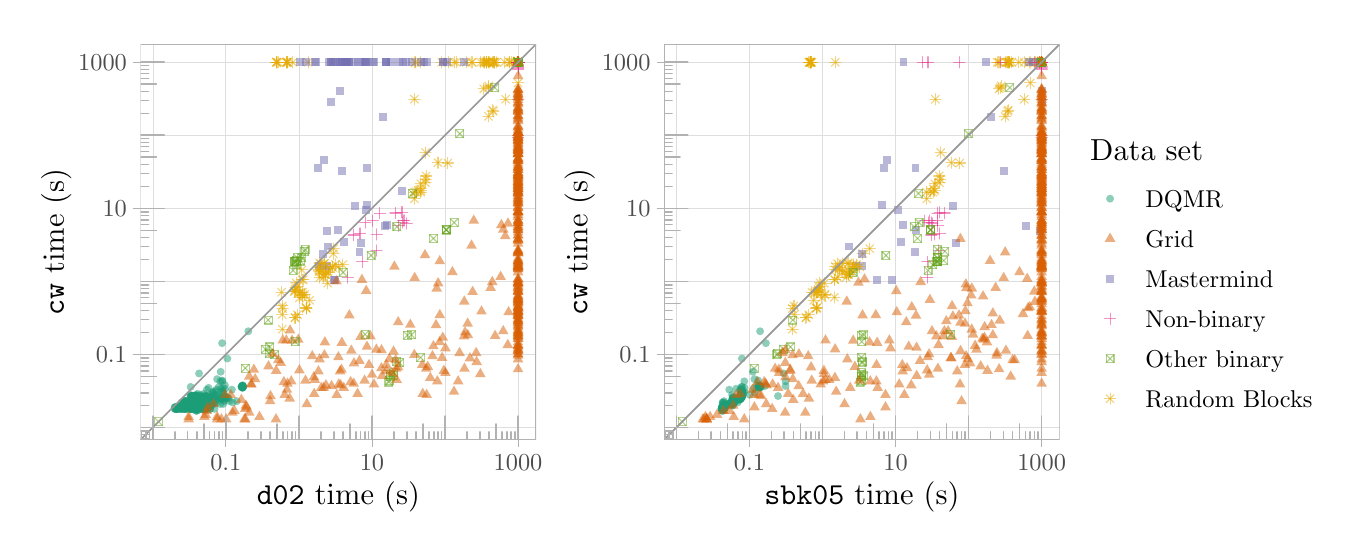
\begin{tikzpicture}[x=1pt,y=1pt]
\definecolor{fillColor}{RGB}{255,255,255}
\path[use as bounding box,fill=fillColor,fill opacity=0.00] (0,0) rectangle (469.75,180.67);
\begin{scope}
\path[clip] (  0.00,  0.51) rectangle (189.19,180.16);
\definecolor{drawColor}{RGB}{255,255,255}
\definecolor{fillColor}{RGB}{255,255,255}

\path[draw=drawColor,line width= 0.6pt,line join=round,line cap=round,fill=fillColor] (  0.00,  0.51) rectangle (189.19,180.16);
\end{scope}
\begin{scope}
\path[clip] ( 40.80, 31.77) rectangle (183.69,174.66);
\definecolor{fillColor}{RGB}{255,255,255}

\path[fill=fillColor] ( 40.80, 31.77) rectangle (183.69,174.66);
\definecolor{drawColor}{gray}{0.87}

\path[draw=drawColor,line width= 0.1pt,line join=round] ( 40.80, 36.17) --
	(183.69, 36.17);

\path[draw=drawColor,line width= 0.1pt,line join=round] ( 40.80, 88.97) --
	(183.69, 88.97);

\path[draw=drawColor,line width= 0.1pt,line join=round] ( 40.80,141.77) --
	(183.69,141.77);

\path[draw=drawColor,line width= 0.1pt,line join=round] ( 45.21, 31.77) --
	( 45.21,174.66);

\path[draw=drawColor,line width= 0.1pt,line join=round] ( 98.00, 31.77) --
	( 98.00,174.66);

\path[draw=drawColor,line width= 0.1pt,line join=round] (150.80, 31.77) --
	(150.80,174.66);

\path[draw=drawColor,line width= 0.3pt,line join=round] ( 40.80, 62.57) --
	(183.69, 62.57);

\path[draw=drawColor,line width= 0.3pt,line join=round] ( 40.80,115.37) --
	(183.69,115.37);

\path[draw=drawColor,line width= 0.3pt,line join=round] ( 40.80,168.17) --
	(183.69,168.17);

\path[draw=drawColor,line width= 0.3pt,line join=round] ( 71.60, 31.77) --
	( 71.60,174.66);

\path[draw=drawColor,line width= 0.3pt,line join=round] (124.40, 31.77) --
	(124.40,174.66);

\path[draw=drawColor,line width= 0.3pt,line join=round] (177.20, 31.77) --
	(177.20,174.66);
\definecolor{drawColor}{RGB}{230,171,2}

\path[draw=drawColor,draw opacity=0.50,line width= 0.4pt,line join=round,line cap=round] ( 92.54,166.74) -- ( 95.39,169.59);

\path[draw=drawColor,draw opacity=0.50,line width= 0.4pt,line join=round,line cap=round] ( 92.54,169.59) -- ( 95.39,166.74);

\path[draw=drawColor,draw opacity=0.50,line width= 0.4pt,line join=round,line cap=round] ( 91.95,168.17) -- ( 95.98,168.17);

\path[draw=drawColor,draw opacity=0.50,line width= 0.4pt,line join=round,line cap=round] ( 93.96,166.15) -- ( 93.96,170.18);

\path[draw=drawColor,draw opacity=0.50,line width= 0.4pt,line join=round,line cap=round] ( 92.07,166.74) -- ( 94.92,169.59);

\path[draw=drawColor,draw opacity=0.50,line width= 0.4pt,line join=round,line cap=round] ( 92.07,169.59) -- ( 94.92,166.74);

\path[draw=drawColor,draw opacity=0.50,line width= 0.4pt,line join=round,line cap=round] ( 91.48,168.17) -- ( 95.51,168.17);

\path[draw=drawColor,draw opacity=0.50,line width= 0.4pt,line join=round,line cap=round] ( 93.50,166.15) -- ( 93.50,170.18);

\path[draw=drawColor,draw opacity=0.50,line width= 0.4pt,line join=round,line cap=round] ( 92.29,166.74) -- ( 95.14,169.59);

\path[draw=drawColor,draw opacity=0.50,line width= 0.4pt,line join=round,line cap=round] ( 92.29,169.59) -- ( 95.14,166.74);

\path[draw=drawColor,draw opacity=0.50,line width= 0.4pt,line join=round,line cap=round] ( 91.70,168.17) -- ( 95.73,168.17);

\path[draw=drawColor,draw opacity=0.50,line width= 0.4pt,line join=round,line cap=round] ( 93.72,166.15) -- ( 93.72,170.18);

\path[draw=drawColor,draw opacity=0.50,line width= 0.4pt,line join=round,line cap=round] ( 94.37,166.74) -- ( 97.22,169.59);

\path[draw=drawColor,draw opacity=0.50,line width= 0.4pt,line join=round,line cap=round] ( 94.37,169.59) -- ( 97.22,166.74);

\path[draw=drawColor,draw opacity=0.50,line width= 0.4pt,line join=round,line cap=round] ( 93.78,168.17) -- ( 97.82,168.17);

\path[draw=drawColor,draw opacity=0.50,line width= 0.4pt,line join=round,line cap=round] ( 95.80,166.15) -- ( 95.80,170.18);

\path[draw=drawColor,draw opacity=0.50,line width= 0.4pt,line join=round,line cap=round] ( 92.07,166.74) -- ( 94.92,169.59);

\path[draw=drawColor,draw opacity=0.50,line width= 0.4pt,line join=round,line cap=round] ( 92.07,169.59) -- ( 94.92,166.74);

\path[draw=drawColor,draw opacity=0.50,line width= 0.4pt,line join=round,line cap=round] ( 91.48,168.17) -- ( 95.51,168.17);

\path[draw=drawColor,draw opacity=0.50,line width= 0.4pt,line join=round,line cap=round] ( 93.50,166.15) -- ( 93.50,170.18);

\path[draw=drawColor,draw opacity=0.50,line width= 0.4pt,line join=round,line cap=round] ( 92.49,166.74) -- ( 95.34,169.59);

\path[draw=drawColor,draw opacity=0.50,line width= 0.4pt,line join=round,line cap=round] ( 92.49,169.59) -- ( 95.34,166.74);

\path[draw=drawColor,draw opacity=0.50,line width= 0.4pt,line join=round,line cap=round] ( 91.90,168.17) -- ( 95.93,168.17);

\path[draw=drawColor,draw opacity=0.50,line width= 0.4pt,line join=round,line cap=round] ( 93.91,166.15) -- ( 93.91,170.18);

\path[draw=drawColor,draw opacity=0.50,line width= 0.4pt,line join=round,line cap=round] ( 90.59, 78.69) -- ( 93.44, 81.54);

\path[draw=drawColor,draw opacity=0.50,line width= 0.4pt,line join=round,line cap=round] ( 90.59, 81.54) -- ( 93.44, 78.69);

\path[draw=drawColor,draw opacity=0.50,line width= 0.4pt,line join=round,line cap=round] ( 89.99, 80.12) -- ( 94.03, 80.12);

\path[draw=drawColor,draw opacity=0.50,line width= 0.4pt,line join=round,line cap=round] ( 92.01, 78.10) -- ( 92.01, 82.13);

\path[draw=drawColor,draw opacity=0.50,line width= 0.4pt,line join=round,line cap=round] ( 90.70, 77.73) -- ( 93.55, 80.59);

\path[draw=drawColor,draw opacity=0.50,line width= 0.4pt,line join=round,line cap=round] ( 90.70, 80.59) -- ( 93.55, 77.73);

\path[draw=drawColor,draw opacity=0.50,line width= 0.4pt,line join=round,line cap=round] ( 90.11, 79.16) -- ( 94.15, 79.16);

\path[draw=drawColor,draw opacity=0.50,line width= 0.4pt,line join=round,line cap=round] ( 92.13, 77.14) -- ( 92.13, 81.18);

\path[draw=drawColor,draw opacity=0.50,line width= 0.4pt,line join=round,line cap=round] ( 90.60, 70.29) -- ( 93.46, 73.14);

\path[draw=drawColor,draw opacity=0.50,line width= 0.4pt,line join=round,line cap=round] ( 90.60, 73.14) -- ( 93.46, 70.29);

\path[draw=drawColor,draw opacity=0.50,line width= 0.4pt,line join=round,line cap=round] ( 90.01, 71.71) -- ( 94.05, 71.71);

\path[draw=drawColor,draw opacity=0.50,line width= 0.4pt,line join=round,line cap=round] ( 92.03, 69.70) -- ( 92.03, 73.73);

\path[draw=drawColor,draw opacity=0.50,line width= 0.4pt,line join=round,line cap=round] (100.44, 80.73) -- (103.30, 83.58);

\path[draw=drawColor,draw opacity=0.50,line width= 0.4pt,line join=round,line cap=round] (100.44, 83.58) -- (103.30, 80.73);

\path[draw=drawColor,draw opacity=0.50,line width= 0.4pt,line join=round,line cap=round] ( 99.85, 82.16) -- (103.89, 82.16);

\path[draw=drawColor,draw opacity=0.50,line width= 0.4pt,line join=round,line cap=round] (101.87, 80.14) -- (101.87, 84.17);

\path[draw=drawColor,draw opacity=0.50,line width= 0.4pt,line join=round,line cap=round] ( 90.55, 75.60) -- ( 93.40, 78.46);

\path[draw=drawColor,draw opacity=0.50,line width= 0.4pt,line join=round,line cap=round] ( 90.55, 78.46) -- ( 93.40, 75.60);

\path[draw=drawColor,draw opacity=0.50,line width= 0.4pt,line join=round,line cap=round] ( 89.96, 77.03) -- ( 93.99, 77.03);

\path[draw=drawColor,draw opacity=0.50,line width= 0.4pt,line join=round,line cap=round] ( 91.97, 75.01) -- ( 91.97, 79.05);

\path[draw=drawColor,draw opacity=0.50,line width= 0.4pt,line join=round,line cap=round] ( 89.04,166.74) -- ( 91.89,169.59);

\path[draw=drawColor,draw opacity=0.50,line width= 0.4pt,line join=round,line cap=round] ( 89.04,169.59) -- ( 91.89,166.74);

\path[draw=drawColor,draw opacity=0.50,line width= 0.4pt,line join=round,line cap=round] ( 88.44,168.17) -- ( 92.48,168.17);

\path[draw=drawColor,draw opacity=0.50,line width= 0.4pt,line join=round,line cap=round] ( 90.46,166.15) -- ( 90.46,170.18);

\path[draw=drawColor,draw opacity=0.50,line width= 0.4pt,line join=round,line cap=round] ( 88.42,166.74) -- ( 91.27,169.59);

\path[draw=drawColor,draw opacity=0.50,line width= 0.4pt,line join=round,line cap=round] ( 88.42,169.59) -- ( 91.27,166.74);

\path[draw=drawColor,draw opacity=0.50,line width= 0.4pt,line join=round,line cap=round] ( 87.83,168.17) -- ( 91.87,168.17);

\path[draw=drawColor,draw opacity=0.50,line width= 0.4pt,line join=round,line cap=round] ( 89.85,166.15) -- ( 89.85,170.18);

\path[draw=drawColor,draw opacity=0.50,line width= 0.4pt,line join=round,line cap=round] ( 99.90,166.74) -- (102.75,169.59);

\path[draw=drawColor,draw opacity=0.50,line width= 0.4pt,line join=round,line cap=round] ( 99.90,169.59) -- (102.75,166.74);

\path[draw=drawColor,draw opacity=0.50,line width= 0.4pt,line join=round,line cap=round] ( 99.31,168.17) -- (103.34,168.17);

\path[draw=drawColor,draw opacity=0.50,line width= 0.4pt,line join=round,line cap=round] (101.32,166.15) -- (101.32,170.18);

\path[draw=drawColor,draw opacity=0.50,line width= 0.4pt,line join=round,line cap=round] ( 88.49,166.74) -- ( 91.34,169.59);

\path[draw=drawColor,draw opacity=0.50,line width= 0.4pt,line join=round,line cap=round] ( 88.49,169.59) -- ( 91.34,166.74);

\path[draw=drawColor,draw opacity=0.50,line width= 0.4pt,line join=round,line cap=round] ( 87.90,168.17) -- ( 91.94,168.17);

\path[draw=drawColor,draw opacity=0.50,line width= 0.4pt,line join=round,line cap=round] ( 89.92,166.15) -- ( 89.92,170.18);

\path[draw=drawColor,draw opacity=0.50,line width= 0.4pt,line join=round,line cap=round] ( 88.54,166.74) -- ( 91.39,169.59);

\path[draw=drawColor,draw opacity=0.50,line width= 0.4pt,line join=round,line cap=round] ( 88.54,169.59) -- ( 91.39,166.74);

\path[draw=drawColor,draw opacity=0.50,line width= 0.4pt,line join=round,line cap=round] ( 87.95,168.17) -- ( 91.98,168.17);

\path[draw=drawColor,draw opacity=0.50,line width= 0.4pt,line join=round,line cap=round] ( 89.96,166.15) -- ( 89.96,170.18);

\path[draw=drawColor,draw opacity=0.50,line width= 0.4pt,line join=round,line cap=round] ( 95.57, 87.03) -- ( 98.42, 89.88);

\path[draw=drawColor,draw opacity=0.50,line width= 0.4pt,line join=round,line cap=round] ( 95.57, 89.88) -- ( 98.42, 87.03);

\path[draw=drawColor,draw opacity=0.50,line width= 0.4pt,line join=round,line cap=round] ( 94.98, 88.45) -- ( 99.01, 88.45);

\path[draw=drawColor,draw opacity=0.50,line width= 0.4pt,line join=round,line cap=round] ( 97.00, 86.44) -- ( 97.00, 90.47);

\path[draw=drawColor,draw opacity=0.50,line width= 0.4pt,line join=round,line cap=round] ( 94.85, 83.79) -- ( 97.70, 86.65);

\path[draw=drawColor,draw opacity=0.50,line width= 0.4pt,line join=round,line cap=round] ( 94.85, 86.65) -- ( 97.70, 83.79);

\path[draw=drawColor,draw opacity=0.50,line width= 0.4pt,line join=round,line cap=round] ( 94.26, 85.22) -- ( 98.29, 85.22);

\path[draw=drawColor,draw opacity=0.50,line width= 0.4pt,line join=round,line cap=round] ( 96.27, 83.20) -- ( 96.27, 87.24);

\path[draw=drawColor,draw opacity=0.50,line width= 0.4pt,line join=round,line cap=round] ( 95.24, 84.62) -- ( 98.09, 87.47);

\path[draw=drawColor,draw opacity=0.50,line width= 0.4pt,line join=round,line cap=round] ( 95.24, 87.47) -- ( 98.09, 84.62);

\path[draw=drawColor,draw opacity=0.50,line width= 0.4pt,line join=round,line cap=round] ( 94.65, 86.05) -- ( 98.68, 86.05);

\path[draw=drawColor,draw opacity=0.50,line width= 0.4pt,line join=round,line cap=round] ( 96.67, 84.03) -- ( 96.67, 88.06);

\path[draw=drawColor,draw opacity=0.50,line width= 0.4pt,line join=round,line cap=round] (104.21, 92.69) -- (107.06, 95.55);

\path[draw=drawColor,draw opacity=0.50,line width= 0.4pt,line join=round,line cap=round] (104.21, 95.55) -- (107.06, 92.69);

\path[draw=drawColor,draw opacity=0.50,line width= 0.4pt,line join=round,line cap=round] (103.62, 94.12) -- (107.65, 94.12);

\path[draw=drawColor,draw opacity=0.50,line width= 0.4pt,line join=round,line cap=round] (105.64, 92.10) -- (105.64, 96.14);

\path[draw=drawColor,draw opacity=0.50,line width= 0.4pt,line join=round,line cap=round] ( 95.16, 84.08) -- ( 98.02, 86.93);

\path[draw=drawColor,draw opacity=0.50,line width= 0.4pt,line join=round,line cap=round] ( 95.16, 86.93) -- ( 98.02, 84.08);

\path[draw=drawColor,draw opacity=0.50,line width= 0.4pt,line join=round,line cap=round] ( 94.57, 85.50) -- ( 98.61, 85.50);

\path[draw=drawColor,draw opacity=0.50,line width= 0.4pt,line join=round,line cap=round] ( 96.59, 83.48) -- ( 96.59, 87.52);

\path[draw=drawColor,draw opacity=0.50,line width= 0.4pt,line join=round,line cap=round] ( 96.16, 85.67) -- ( 99.01, 88.52);

\path[draw=drawColor,draw opacity=0.50,line width= 0.4pt,line join=round,line cap=round] ( 96.16, 88.52) -- ( 99.01, 85.67);

\path[draw=drawColor,draw opacity=0.50,line width= 0.4pt,line join=round,line cap=round] ( 95.57, 87.09) -- ( 99.60, 87.09);

\path[draw=drawColor,draw opacity=0.50,line width= 0.4pt,line join=round,line cap=round] ( 97.58, 85.08) -- ( 97.58, 89.11);

\path[draw=drawColor,draw opacity=0.50,line width= 0.4pt,line join=round,line cap=round] (106.97, 86.93) -- (109.82, 89.78);

\path[draw=drawColor,draw opacity=0.50,line width= 0.4pt,line join=round,line cap=round] (106.97, 89.78) -- (109.82, 86.93);

\path[draw=drawColor,draw opacity=0.50,line width= 0.4pt,line join=round,line cap=round] (106.38, 88.36) -- (110.42, 88.36);

\path[draw=drawColor,draw opacity=0.50,line width= 0.4pt,line join=round,line cap=round] (108.40, 86.34) -- (108.40, 90.37);

\path[draw=drawColor,draw opacity=0.50,line width= 0.4pt,line join=round,line cap=round] ( 95.27, 74.52) -- ( 98.12, 77.37);

\path[draw=drawColor,draw opacity=0.50,line width= 0.4pt,line join=round,line cap=round] ( 95.27, 77.37) -- ( 98.12, 74.52);

\path[draw=drawColor,draw opacity=0.50,line width= 0.4pt,line join=round,line cap=round] ( 94.68, 75.94) -- ( 98.71, 75.94);

\path[draw=drawColor,draw opacity=0.50,line width= 0.4pt,line join=round,line cap=round] ( 96.69, 73.92) -- ( 96.69, 77.96);

\path[draw=drawColor,draw opacity=0.50,line width= 0.4pt,line join=round,line cap=round] ( 96.05, 75.51) -- ( 98.90, 78.36);

\path[draw=drawColor,draw opacity=0.50,line width= 0.4pt,line join=round,line cap=round] ( 96.05, 78.36) -- ( 98.90, 75.51);

\path[draw=drawColor,draw opacity=0.50,line width= 0.4pt,line join=round,line cap=round] ( 95.46, 76.93) -- ( 99.49, 76.93);

\path[draw=drawColor,draw opacity=0.50,line width= 0.4pt,line join=round,line cap=round] ( 97.48, 74.92) -- ( 97.48, 78.95);

\path[draw=drawColor,draw opacity=0.50,line width= 0.4pt,line join=round,line cap=round] ( 95.18, 74.37) -- ( 98.03, 77.22);

\path[draw=drawColor,draw opacity=0.50,line width= 0.4pt,line join=round,line cap=round] ( 95.18, 77.22) -- ( 98.03, 74.37);

\path[draw=drawColor,draw opacity=0.50,line width= 0.4pt,line join=round,line cap=round] ( 94.58, 75.80) -- ( 98.62, 75.80);

\path[draw=drawColor,draw opacity=0.50,line width= 0.4pt,line join=round,line cap=round] ( 96.60, 73.78) -- ( 96.60, 77.82);

\path[draw=drawColor,draw opacity=0.50,line width= 0.4pt,line join=round,line cap=round] ( 90.33, 83.65) -- ( 93.18, 86.50);

\path[draw=drawColor,draw opacity=0.50,line width= 0.4pt,line join=round,line cap=round] ( 90.33, 86.50) -- ( 93.18, 83.65);

\path[draw=drawColor,draw opacity=0.50,line width= 0.4pt,line join=round,line cap=round] ( 89.74, 85.08) -- ( 93.78, 85.08);

\path[draw=drawColor,draw opacity=0.50,line width= 0.4pt,line join=round,line cap=round] ( 91.76, 83.06) -- ( 91.76, 87.09);

\path[draw=drawColor,draw opacity=0.50,line width= 0.4pt,line join=round,line cap=round] ( 97.90, 83.65) -- (100.75, 86.50);

\path[draw=drawColor,draw opacity=0.50,line width= 0.4pt,line join=round,line cap=round] ( 97.90, 86.50) -- (100.75, 83.65);

\path[draw=drawColor,draw opacity=0.50,line width= 0.4pt,line join=round,line cap=round] ( 97.31, 85.08) -- (101.34, 85.08);

\path[draw=drawColor,draw opacity=0.50,line width= 0.4pt,line join=round,line cap=round] ( 99.32, 83.06) -- ( 99.32, 87.09);

\path[draw=drawColor,draw opacity=0.50,line width= 0.4pt,line join=round,line cap=round] (106.37, 92.93) -- (109.23, 95.78);

\path[draw=drawColor,draw opacity=0.50,line width= 0.4pt,line join=round,line cap=round] (106.37, 95.78) -- (109.23, 92.93);

\path[draw=drawColor,draw opacity=0.50,line width= 0.4pt,line join=round,line cap=round] (105.78, 94.36) -- (109.82, 94.36);

\path[draw=drawColor,draw opacity=0.50,line width= 0.4pt,line join=round,line cap=round] (107.80, 92.34) -- (107.80, 96.38);

\path[draw=drawColor,draw opacity=0.50,line width= 0.4pt,line join=round,line cap=round] ( 97.28, 83.57) -- (100.13, 86.42);

\path[draw=drawColor,draw opacity=0.50,line width= 0.4pt,line join=round,line cap=round] ( 97.28, 86.42) -- (100.13, 83.57);

\path[draw=drawColor,draw opacity=0.50,line width= 0.4pt,line join=round,line cap=round] ( 96.69, 84.99) -- (100.72, 84.99);

\path[draw=drawColor,draw opacity=0.50,line width= 0.4pt,line join=round,line cap=round] ( 98.70, 82.98) -- ( 98.70, 87.01);

\path[draw=drawColor,draw opacity=0.50,line width= 0.4pt,line join=round,line cap=round] (104.40, 93.97) -- (107.25, 96.82);

\path[draw=drawColor,draw opacity=0.50,line width= 0.4pt,line join=round,line cap=round] (104.40, 96.82) -- (107.25, 93.97);

\path[draw=drawColor,draw opacity=0.50,line width= 0.4pt,line join=round,line cap=round] (103.81, 95.39) -- (107.84, 95.39);

\path[draw=drawColor,draw opacity=0.50,line width= 0.4pt,line join=round,line cap=round] (105.82, 93.37) -- (105.82, 97.41);

\path[draw=drawColor,draw opacity=0.50,line width= 0.4pt,line join=round,line cap=round] ( 96.72, 83.47) -- ( 99.58, 86.32);

\path[draw=drawColor,draw opacity=0.50,line width= 0.4pt,line join=round,line cap=round] ( 96.72, 86.32) -- ( 99.58, 83.47);

\path[draw=drawColor,draw opacity=0.50,line width= 0.4pt,line join=round,line cap=round] ( 96.13, 84.90) -- (100.17, 84.90);

\path[draw=drawColor,draw opacity=0.50,line width= 0.4pt,line join=round,line cap=round] ( 98.15, 82.88) -- ( 98.15, 86.91);

\path[draw=drawColor,draw opacity=0.50,line width= 0.4pt,line join=round,line cap=round] (106.30, 90.02) -- (109.15, 92.87);

\path[draw=drawColor,draw opacity=0.50,line width= 0.4pt,line join=round,line cap=round] (106.30, 92.87) -- (109.15, 90.02);

\path[draw=drawColor,draw opacity=0.50,line width= 0.4pt,line join=round,line cap=round] (105.71, 91.45) -- (109.74, 91.45);

\path[draw=drawColor,draw opacity=0.50,line width= 0.4pt,line join=round,line cap=round] (107.73, 89.43) -- (107.73, 93.46);

\path[draw=drawColor,draw opacity=0.50,line width= 0.4pt,line join=round,line cap=round] (106.15, 90.03) -- (109.00, 92.88);

\path[draw=drawColor,draw opacity=0.50,line width= 0.4pt,line join=round,line cap=round] (106.15, 92.88) -- (109.00, 90.03);

\path[draw=drawColor,draw opacity=0.50,line width= 0.4pt,line join=round,line cap=round] (105.56, 91.45) -- (109.59, 91.45);

\path[draw=drawColor,draw opacity=0.50,line width= 0.4pt,line join=round,line cap=round] (107.58, 89.44) -- (107.58, 93.47);

\path[draw=drawColor,draw opacity=0.50,line width= 0.4pt,line join=round,line cap=round] (109.16, 99.39) -- (112.01,102.25);

\path[draw=drawColor,draw opacity=0.50,line width= 0.4pt,line join=round,line cap=round] (109.16,102.25) -- (112.01, 99.39);

\path[draw=drawColor,draw opacity=0.50,line width= 0.4pt,line join=round,line cap=round] (108.57,100.82) -- (112.60,100.82);

\path[draw=drawColor,draw opacity=0.50,line width= 0.4pt,line join=round,line cap=round] (110.58, 98.80) -- (110.58,102.84);

\path[draw=drawColor,draw opacity=0.50,line width= 0.4pt,line join=round,line cap=round] (105.55, 89.07) -- (108.41, 91.92);

\path[draw=drawColor,draw opacity=0.50,line width= 0.4pt,line join=round,line cap=round] (105.55, 91.92) -- (108.41, 89.07);

\path[draw=drawColor,draw opacity=0.50,line width= 0.4pt,line join=round,line cap=round] (104.96, 90.49) -- (109.00, 90.49);

\path[draw=drawColor,draw opacity=0.50,line width= 0.4pt,line join=round,line cap=round] (106.98, 88.47) -- (106.98, 92.51);

\path[draw=drawColor,draw opacity=0.50,line width= 0.4pt,line join=round,line cap=round] (106.34, 90.97) -- (109.20, 93.82);

\path[draw=drawColor,draw opacity=0.50,line width= 0.4pt,line join=round,line cap=round] (106.34, 93.82) -- (109.20, 90.97);

\path[draw=drawColor,draw opacity=0.50,line width= 0.4pt,line join=round,line cap=round] (105.75, 92.39) -- (109.79, 92.39);

\path[draw=drawColor,draw opacity=0.50,line width= 0.4pt,line join=round,line cap=round] (107.77, 90.38) -- (107.77, 94.41);

\path[draw=drawColor,draw opacity=0.50,line width= 0.4pt,line join=round,line cap=round] (107.30, 90.65) -- (110.15, 93.50);

\path[draw=drawColor,draw opacity=0.50,line width= 0.4pt,line join=round,line cap=round] (107.30, 93.50) -- (110.15, 90.65);

\path[draw=drawColor,draw opacity=0.50,line width= 0.4pt,line join=round,line cap=round] (106.70, 92.07) -- (110.74, 92.07);

\path[draw=drawColor,draw opacity=0.50,line width= 0.4pt,line join=round,line cap=round] (108.72, 90.06) -- (108.72, 94.09);

\path[draw=drawColor,draw opacity=0.50,line width= 0.4pt,line join=round,line cap=round] ( 99.18, 77.95) -- (102.03, 80.80);

\path[draw=drawColor,draw opacity=0.50,line width= 0.4pt,line join=round,line cap=round] ( 99.18, 80.80) -- (102.03, 77.95);

\path[draw=drawColor,draw opacity=0.50,line width= 0.4pt,line join=round,line cap=round] ( 98.59, 79.37) -- (102.62, 79.37);

\path[draw=drawColor,draw opacity=0.50,line width= 0.4pt,line join=round,line cap=round] (100.61, 77.36) -- (100.61, 81.39);

\path[draw=drawColor,draw opacity=0.50,line width= 0.4pt,line join=round,line cap=round] ( 95.47, 85.35) -- ( 98.32, 88.20);

\path[draw=drawColor,draw opacity=0.50,line width= 0.4pt,line join=round,line cap=round] ( 95.47, 88.20) -- ( 98.32, 85.35);

\path[draw=drawColor,draw opacity=0.50,line width= 0.4pt,line join=round,line cap=round] ( 94.88, 86.78) -- ( 98.91, 86.78);

\path[draw=drawColor,draw opacity=0.50,line width= 0.4pt,line join=round,line cap=round] ( 96.90, 84.76) -- ( 96.90, 88.80);

\path[draw=drawColor,draw opacity=0.50,line width= 0.4pt,line join=round,line cap=round] (112.42, 93.62) -- (115.27, 96.47);

\path[draw=drawColor,draw opacity=0.50,line width= 0.4pt,line join=round,line cap=round] (112.42, 96.47) -- (115.27, 93.62);

\path[draw=drawColor,draw opacity=0.50,line width= 0.4pt,line join=round,line cap=round] (111.83, 95.05) -- (115.86, 95.05);

\path[draw=drawColor,draw opacity=0.50,line width= 0.4pt,line join=round,line cap=round] (113.85, 93.03) -- (113.85, 97.06);

\path[draw=drawColor,draw opacity=0.50,line width= 0.4pt,line join=round,line cap=round] ( 99.17, 78.10) -- (102.02, 80.96);

\path[draw=drawColor,draw opacity=0.50,line width= 0.4pt,line join=round,line cap=round] ( 99.17, 80.96) -- (102.02, 78.10);

\path[draw=drawColor,draw opacity=0.50,line width= 0.4pt,line join=round,line cap=round] ( 98.58, 79.53) -- (102.62, 79.53);

\path[draw=drawColor,draw opacity=0.50,line width= 0.4pt,line join=round,line cap=round] (100.60, 77.51) -- (100.60, 81.55);

\path[draw=drawColor,draw opacity=0.50,line width= 0.4pt,line join=round,line cap=round] ( 99.29, 77.79) -- (102.14, 80.64);

\path[draw=drawColor,draw opacity=0.50,line width= 0.4pt,line join=round,line cap=round] ( 99.29, 80.64) -- (102.14, 77.79);

\path[draw=drawColor,draw opacity=0.50,line width= 0.4pt,line join=round,line cap=round] ( 98.70, 79.21) -- (102.73, 79.21);

\path[draw=drawColor,draw opacity=0.50,line width= 0.4pt,line join=round,line cap=round] (100.72, 77.20) -- (100.72, 81.23);

\path[draw=drawColor,draw opacity=0.50,line width= 0.4pt,line join=round,line cap=round] (109.00, 97.57) -- (111.86,100.42);

\path[draw=drawColor,draw opacity=0.50,line width= 0.4pt,line join=round,line cap=round] (109.00,100.42) -- (111.86, 97.57);

\path[draw=drawColor,draw opacity=0.50,line width= 0.4pt,line join=round,line cap=round] (108.41, 99.00) -- (112.45, 99.00);

\path[draw=drawColor,draw opacity=0.50,line width= 0.4pt,line join=round,line cap=round] (110.43, 96.98) -- (110.43,101.01);

\path[draw=drawColor,draw opacity=0.50,line width= 0.4pt,line join=round,line cap=round] ( 97.75, 88.20) -- (100.61, 91.05);

\path[draw=drawColor,draw opacity=0.50,line width= 0.4pt,line join=round,line cap=round] ( 97.75, 91.05) -- (100.61, 88.20);

\path[draw=drawColor,draw opacity=0.50,line width= 0.4pt,line join=round,line cap=round] ( 97.16, 89.63) -- (101.20, 89.63);

\path[draw=drawColor,draw opacity=0.50,line width= 0.4pt,line join=round,line cap=round] ( 99.18, 87.61) -- ( 99.18, 91.64);

\path[draw=drawColor,draw opacity=0.50,line width= 0.4pt,line join=round,line cap=round] ( 98.15, 88.16) -- (101.00, 91.01);

\path[draw=drawColor,draw opacity=0.50,line width= 0.4pt,line join=round,line cap=round] ( 98.15, 91.01) -- (101.00, 88.16);

\path[draw=drawColor,draw opacity=0.50,line width= 0.4pt,line join=round,line cap=round] ( 97.56, 89.58) -- (101.59, 89.58);

\path[draw=drawColor,draw opacity=0.50,line width= 0.4pt,line join=round,line cap=round] ( 99.58, 87.57) -- ( 99.58, 91.60);

\path[draw=drawColor,draw opacity=0.50,line width= 0.4pt,line join=round,line cap=round] ( 97.67, 91.71) -- (100.52, 94.56);

\path[draw=drawColor,draw opacity=0.50,line width= 0.4pt,line join=round,line cap=round] ( 97.67, 94.56) -- (100.52, 91.71);

\path[draw=drawColor,draw opacity=0.50,line width= 0.4pt,line join=round,line cap=round] ( 97.08, 93.13) -- (101.11, 93.13);

\path[draw=drawColor,draw opacity=0.50,line width= 0.4pt,line join=round,line cap=round] ( 99.10, 91.12) -- ( 99.10, 95.15);

\path[draw=drawColor,draw opacity=0.50,line width= 0.4pt,line join=round,line cap=round] (104.12, 88.96) -- (106.97, 91.82);

\path[draw=drawColor,draw opacity=0.50,line width= 0.4pt,line join=round,line cap=round] (104.12, 91.82) -- (106.97, 88.96);

\path[draw=drawColor,draw opacity=0.50,line width= 0.4pt,line join=round,line cap=round] (103.53, 90.39) -- (107.56, 90.39);

\path[draw=drawColor,draw opacity=0.50,line width= 0.4pt,line join=round,line cap=round] (105.55, 88.37) -- (105.55, 92.41);

\path[draw=drawColor,draw opacity=0.50,line width= 0.4pt,line join=round,line cap=round] (175.77,166.74) -- (178.63,169.59);

\path[draw=drawColor,draw opacity=0.50,line width= 0.4pt,line join=round,line cap=round] (175.77,169.59) -- (178.63,166.74);

\path[draw=drawColor,draw opacity=0.50,line width= 0.4pt,line join=round,line cap=round] (175.18,168.17) -- (179.22,168.17);

\path[draw=drawColor,draw opacity=0.50,line width= 0.4pt,line join=round,line cap=round] (177.20,166.15) -- (177.20,170.18);

\path[draw=drawColor,draw opacity=0.50,line width= 0.4pt,line join=round,line cap=round] (138.73,166.74) -- (141.59,169.59);

\path[draw=drawColor,draw opacity=0.50,line width= 0.4pt,line join=round,line cap=round] (138.73,169.59) -- (141.59,166.74);

\path[draw=drawColor,draw opacity=0.50,line width= 0.4pt,line join=round,line cap=round] (138.14,168.17) -- (142.18,168.17);

\path[draw=drawColor,draw opacity=0.50,line width= 0.4pt,line join=round,line cap=round] (140.16,166.15) -- (140.16,170.18);

\path[draw=drawColor,draw opacity=0.50,line width= 0.4pt,line join=round,line cap=round] (148.17,166.74) -- (151.02,169.59);

\path[draw=drawColor,draw opacity=0.50,line width= 0.4pt,line join=round,line cap=round] (148.17,169.59) -- (151.02,166.74);

\path[draw=drawColor,draw opacity=0.50,line width= 0.4pt,line join=round,line cap=round] (147.58,168.17) -- (151.61,168.17);

\path[draw=drawColor,draw opacity=0.50,line width= 0.4pt,line join=round,line cap=round] (149.60,166.15) -- (149.60,170.18);

\path[draw=drawColor,draw opacity=0.50,line width= 0.4pt,line join=round,line cap=round] (175.77,166.74) -- (178.63,169.59);

\path[draw=drawColor,draw opacity=0.50,line width= 0.4pt,line join=round,line cap=round] (175.77,169.59) -- (178.63,166.74);

\path[draw=drawColor,draw opacity=0.50,line width= 0.4pt,line join=round,line cap=round] (175.18,168.17) -- (179.22,168.17);

\path[draw=drawColor,draw opacity=0.50,line width= 0.4pt,line join=round,line cap=round] (177.20,166.15) -- (177.20,170.18);

\path[draw=drawColor,draw opacity=0.50,line width= 0.4pt,line join=round,line cap=round] (138.53,166.74) -- (141.39,169.59);

\path[draw=drawColor,draw opacity=0.50,line width= 0.4pt,line join=round,line cap=round] (138.53,169.59) -- (141.39,166.74);

\path[draw=drawColor,draw opacity=0.50,line width= 0.4pt,line join=round,line cap=round] (137.94,168.17) -- (141.98,168.17);

\path[draw=drawColor,draw opacity=0.50,line width= 0.4pt,line join=round,line cap=round] (139.96,166.15) -- (139.96,170.18);

\path[draw=drawColor,draw opacity=0.50,line width= 0.4pt,line join=round,line cap=round] (175.77,166.74) -- (178.63,169.59);

\path[draw=drawColor,draw opacity=0.50,line width= 0.4pt,line join=round,line cap=round] (175.77,169.59) -- (178.63,166.74);

\path[draw=drawColor,draw opacity=0.50,line width= 0.4pt,line join=round,line cap=round] (175.18,168.17) -- (179.22,168.17);

\path[draw=drawColor,draw opacity=0.50,line width= 0.4pt,line join=round,line cap=round] (177.20,166.15) -- (177.20,170.18);

\path[draw=drawColor,draw opacity=0.50,line width= 0.4pt,line join=round,line cap=round] (138.32,153.40) -- (141.17,156.26);

\path[draw=drawColor,draw opacity=0.50,line width= 0.4pt,line join=round,line cap=round] (138.32,156.26) -- (141.17,153.40);

\path[draw=drawColor,draw opacity=0.50,line width= 0.4pt,line join=round,line cap=round] (137.72,154.83) -- (141.76,154.83);

\path[draw=drawColor,draw opacity=0.50,line width= 0.4pt,line join=round,line cap=round] (139.74,152.81) -- (139.74,156.85);

\path[draw=drawColor,draw opacity=0.50,line width= 0.4pt,line join=round,line cap=round] (146.82,130.46) -- (149.68,133.31);

\path[draw=drawColor,draw opacity=0.50,line width= 0.4pt,line join=round,line cap=round] (146.82,133.31) -- (149.68,130.46);

\path[draw=drawColor,draw opacity=0.50,line width= 0.4pt,line join=round,line cap=round] (146.23,131.89) -- (150.27,131.89);

\path[draw=drawColor,draw opacity=0.50,line width= 0.4pt,line join=round,line cap=round] (148.25,129.87) -- (148.25,133.90);

\path[draw=drawColor,draw opacity=0.50,line width= 0.4pt,line join=round,line cap=round] (138.31,117.39) -- (141.16,120.25);

\path[draw=drawColor,draw opacity=0.50,line width= 0.4pt,line join=round,line cap=round] (138.31,120.25) -- (141.16,117.39);

\path[draw=drawColor,draw opacity=0.50,line width= 0.4pt,line join=round,line cap=round] (137.72,118.82) -- (141.75,118.82);

\path[draw=drawColor,draw opacity=0.50,line width= 0.4pt,line join=round,line cap=round] (139.74,116.80) -- (139.74,120.84);

\path[draw=drawColor,draw opacity=0.50,line width= 0.4pt,line join=round,line cap=round] (138.88,120.01) -- (141.73,122.86);

\path[draw=drawColor,draw opacity=0.50,line width= 0.4pt,line join=round,line cap=round] (138.88,122.86) -- (141.73,120.01);

\path[draw=drawColor,draw opacity=0.50,line width= 0.4pt,line join=round,line cap=round] (138.29,121.43) -- (142.32,121.43);

\path[draw=drawColor,draw opacity=0.50,line width= 0.4pt,line join=round,line cap=round] (140.31,119.42) -- (140.31,123.45);

\path[draw=drawColor,draw opacity=0.50,line width= 0.4pt,line join=round,line cap=round] (138.37,119.83) -- (141.22,122.68);

\path[draw=drawColor,draw opacity=0.50,line width= 0.4pt,line join=round,line cap=round] (138.37,122.68) -- (141.22,119.83);

\path[draw=drawColor,draw opacity=0.50,line width= 0.4pt,line join=round,line cap=round] (137.78,121.26) -- (141.82,121.26);

\path[draw=drawColor,draw opacity=0.50,line width= 0.4pt,line join=round,line cap=round] (139.80,119.24) -- (139.80,123.28);

\path[draw=drawColor,draw opacity=0.50,line width= 0.4pt,line join=round,line cap=round] (159.26,166.74) -- (162.11,169.59);

\path[draw=drawColor,draw opacity=0.50,line width= 0.4pt,line join=round,line cap=round] (159.26,169.59) -- (162.11,166.74);

\path[draw=drawColor,draw opacity=0.50,line width= 0.4pt,line join=round,line cap=round] (158.67,168.17) -- (162.70,168.17);

\path[draw=drawColor,draw opacity=0.50,line width= 0.4pt,line join=round,line cap=round] (160.69,166.15) -- (160.69,170.18);

\path[draw=drawColor,draw opacity=0.50,line width= 0.4pt,line join=round,line cap=round] (175.77,166.74) -- (178.63,169.59);

\path[draw=drawColor,draw opacity=0.50,line width= 0.4pt,line join=round,line cap=round] (175.77,169.59) -- (178.63,166.74);

\path[draw=drawColor,draw opacity=0.50,line width= 0.4pt,line join=round,line cap=round] (175.18,168.17) -- (179.22,168.17);

\path[draw=drawColor,draw opacity=0.50,line width= 0.4pt,line join=round,line cap=round] (177.20,166.15) -- (177.20,170.18);

\path[draw=drawColor,draw opacity=0.50,line width= 0.4pt,line join=round,line cap=round] (152.65,166.74) -- (155.50,169.59);

\path[draw=drawColor,draw opacity=0.50,line width= 0.4pt,line join=round,line cap=round] (152.65,169.59) -- (155.50,166.74);

\path[draw=drawColor,draw opacity=0.50,line width= 0.4pt,line join=round,line cap=round] (152.06,168.17) -- (156.09,168.17);

\path[draw=drawColor,draw opacity=0.50,line width= 0.4pt,line join=round,line cap=round] (154.08,166.15) -- (154.08,170.18);

\path[draw=drawColor,draw opacity=0.50,line width= 0.4pt,line join=round,line cap=round] (164.98,166.74) -- (167.83,169.59);

\path[draw=drawColor,draw opacity=0.50,line width= 0.4pt,line join=round,line cap=round] (164.98,169.59) -- (167.83,166.74);

\path[draw=drawColor,draw opacity=0.50,line width= 0.4pt,line join=round,line cap=round] (164.39,168.17) -- (168.42,168.17);

\path[draw=drawColor,draw opacity=0.50,line width= 0.4pt,line join=round,line cap=round] (166.40,166.15) -- (166.40,170.18);

\path[draw=drawColor,draw opacity=0.50,line width= 0.4pt,line join=round,line cap=round] (157.06,166.74) -- (159.91,169.59);

\path[draw=drawColor,draw opacity=0.50,line width= 0.4pt,line join=round,line cap=round] (157.06,169.59) -- (159.91,166.74);

\path[draw=drawColor,draw opacity=0.50,line width= 0.4pt,line join=round,line cap=round] (156.47,168.17) -- (160.51,168.17);

\path[draw=drawColor,draw opacity=0.50,line width= 0.4pt,line join=round,line cap=round] (158.49,166.15) -- (158.49,170.18);

\path[draw=drawColor,draw opacity=0.50,line width= 0.4pt,line join=round,line cap=round] (175.77,166.74) -- (178.63,169.59);

\path[draw=drawColor,draw opacity=0.50,line width= 0.4pt,line join=round,line cap=round] (175.77,169.59) -- (178.63,166.74);

\path[draw=drawColor,draw opacity=0.50,line width= 0.4pt,line join=round,line cap=round] (175.18,168.17) -- (179.22,168.17);

\path[draw=drawColor,draw opacity=0.50,line width= 0.4pt,line join=round,line cap=round] (177.20,166.15) -- (177.20,170.18);

\path[draw=drawColor,draw opacity=0.50,line width= 0.4pt,line join=round,line cap=round] (150.50,166.74) -- (153.36,169.59);

\path[draw=drawColor,draw opacity=0.50,line width= 0.4pt,line join=round,line cap=round] (150.50,169.59) -- (153.36,166.74);

\path[draw=drawColor,draw opacity=0.50,line width= 0.4pt,line join=round,line cap=round] (149.91,168.17) -- (153.95,168.17);

\path[draw=drawColor,draw opacity=0.50,line width= 0.4pt,line join=round,line cap=round] (151.93,166.15) -- (151.93,170.18);

\path[draw=drawColor,draw opacity=0.50,line width= 0.4pt,line join=round,line cap=round] (140.44,166.74) -- (143.29,169.59);

\path[draw=drawColor,draw opacity=0.50,line width= 0.4pt,line join=round,line cap=round] (140.44,169.59) -- (143.29,166.74);

\path[draw=drawColor,draw opacity=0.50,line width= 0.4pt,line join=round,line cap=round] (139.85,168.17) -- (143.88,168.17);

\path[draw=drawColor,draw opacity=0.50,line width= 0.4pt,line join=round,line cap=round] (141.87,166.15) -- (141.87,170.18);

\path[draw=drawColor,draw opacity=0.50,line width= 0.4pt,line join=round,line cap=round] (175.77,166.74) -- (178.63,169.59);

\path[draw=drawColor,draw opacity=0.50,line width= 0.4pt,line join=round,line cap=round] (175.77,169.59) -- (178.63,166.74);

\path[draw=drawColor,draw opacity=0.50,line width= 0.4pt,line join=round,line cap=round] (175.18,168.17) -- (179.22,168.17);

\path[draw=drawColor,draw opacity=0.50,line width= 0.4pt,line join=round,line cap=round] (177.20,166.15) -- (177.20,170.18);

\path[draw=drawColor,draw opacity=0.50,line width= 0.4pt,line join=round,line cap=round] (175.77,166.74) -- (178.63,169.59);

\path[draw=drawColor,draw opacity=0.50,line width= 0.4pt,line join=round,line cap=round] (175.77,169.59) -- (178.63,166.74);

\path[draw=drawColor,draw opacity=0.50,line width= 0.4pt,line join=round,line cap=round] (175.18,168.17) -- (179.22,168.17);

\path[draw=drawColor,draw opacity=0.50,line width= 0.4pt,line join=round,line cap=round] (177.20,166.15) -- (177.20,170.18);

\path[draw=drawColor,draw opacity=0.50,line width= 0.4pt,line join=round,line cap=round] (175.77,166.74) -- (178.63,169.59);

\path[draw=drawColor,draw opacity=0.50,line width= 0.4pt,line join=round,line cap=round] (175.77,169.59) -- (178.63,166.74);

\path[draw=drawColor,draw opacity=0.50,line width= 0.4pt,line join=round,line cap=round] (175.18,168.17) -- (179.22,168.17);

\path[draw=drawColor,draw opacity=0.50,line width= 0.4pt,line join=round,line cap=round] (177.20,166.15) -- (177.20,170.18);

\path[draw=drawColor,draw opacity=0.50,line width= 0.4pt,line join=round,line cap=round] (150.41,130.32) -- (153.26,133.17);

\path[draw=drawColor,draw opacity=0.50,line width= 0.4pt,line join=round,line cap=round] (150.41,133.17) -- (153.26,130.32);

\path[draw=drawColor,draw opacity=0.50,line width= 0.4pt,line join=round,line cap=round] (149.81,131.75) -- (153.85,131.75);

\path[draw=drawColor,draw opacity=0.50,line width= 0.4pt,line join=round,line cap=round] (151.83,129.73) -- (151.83,133.76);

\path[draw=drawColor,draw opacity=0.50,line width= 0.4pt,line join=round,line cap=round] (140.65,121.06) -- (143.50,123.91);

\path[draw=drawColor,draw opacity=0.50,line width= 0.4pt,line join=round,line cap=round] (140.65,123.91) -- (143.50,121.06);

\path[draw=drawColor,draw opacity=0.50,line width= 0.4pt,line join=round,line cap=round] (140.06,122.49) -- (144.09,122.49);

\path[draw=drawColor,draw opacity=0.50,line width= 0.4pt,line join=round,line cap=round] (142.07,120.47) -- (142.07,124.50);

\path[draw=drawColor,draw opacity=0.50,line width= 0.4pt,line join=round,line cap=round] (140.68,120.30) -- (143.54,123.15);

\path[draw=drawColor,draw opacity=0.50,line width= 0.4pt,line join=round,line cap=round] (140.68,123.15) -- (143.54,120.30);

\path[draw=drawColor,draw opacity=0.50,line width= 0.4pt,line join=round,line cap=round] (140.09,121.73) -- (144.13,121.73);

\path[draw=drawColor,draw opacity=0.50,line width= 0.4pt,line join=round,line cap=round] (142.11,119.71) -- (142.11,123.74);

\path[draw=drawColor,draw opacity=0.50,line width= 0.4pt,line join=round,line cap=round] (140.66,122.82) -- (143.51,125.67);

\path[draw=drawColor,draw opacity=0.50,line width= 0.4pt,line join=round,line cap=round] (140.66,125.67) -- (143.51,122.82);

\path[draw=drawColor,draw opacity=0.50,line width= 0.4pt,line join=round,line cap=round] (140.06,124.25) -- (144.10,124.25);

\path[draw=drawColor,draw opacity=0.50,line width= 0.4pt,line join=round,line cap=round] (142.08,122.23) -- (142.08,126.26);

\path[draw=drawColor,draw opacity=0.50,line width= 0.4pt,line join=round,line cap=round] (140.61,119.76) -- (143.46,122.62);

\path[draw=drawColor,draw opacity=0.50,line width= 0.4pt,line join=round,line cap=round] (140.61,122.62) -- (143.46,119.76);

\path[draw=drawColor,draw opacity=0.50,line width= 0.4pt,line join=round,line cap=round] (140.02,121.19) -- (144.05,121.19);

\path[draw=drawColor,draw opacity=0.50,line width= 0.4pt,line join=round,line cap=round] (142.03,119.17) -- (142.03,123.21);

\path[draw=drawColor,draw opacity=0.50,line width= 0.4pt,line join=round,line cap=round] (175.77,166.74) -- (178.63,169.59);

\path[draw=drawColor,draw opacity=0.50,line width= 0.4pt,line join=round,line cap=round] (175.77,169.59) -- (178.63,166.74);

\path[draw=drawColor,draw opacity=0.50,line width= 0.4pt,line join=round,line cap=round] (175.18,168.17) -- (179.22,168.17);

\path[draw=drawColor,draw opacity=0.50,line width= 0.4pt,line join=round,line cap=round] (177.20,166.15) -- (177.20,170.18);

\path[draw=drawColor,draw opacity=0.50,line width= 0.4pt,line join=round,line cap=round] (173.29,166.74) -- (176.14,169.59);

\path[draw=drawColor,draw opacity=0.50,line width= 0.4pt,line join=round,line cap=round] (173.29,169.59) -- (176.14,166.74);

\path[draw=drawColor,draw opacity=0.50,line width= 0.4pt,line join=round,line cap=round] (172.70,168.17) -- (176.73,168.17);

\path[draw=drawColor,draw opacity=0.50,line width= 0.4pt,line join=round,line cap=round] (174.71,166.15) -- (174.71,170.18);

\path[draw=drawColor,draw opacity=0.50,line width= 0.4pt,line join=round,line cap=round] (153.45,166.74) -- (156.30,169.59);

\path[draw=drawColor,draw opacity=0.50,line width= 0.4pt,line join=round,line cap=round] (153.45,169.59) -- (156.30,166.74);

\path[draw=drawColor,draw opacity=0.50,line width= 0.4pt,line join=round,line cap=round] (152.86,168.17) -- (156.89,168.17);

\path[draw=drawColor,draw opacity=0.50,line width= 0.4pt,line join=round,line cap=round] (154.88,166.15) -- (154.88,170.18);

\path[draw=drawColor,draw opacity=0.50,line width= 0.4pt,line join=round,line cap=round] (172.80,166.74) -- (175.65,169.59);

\path[draw=drawColor,draw opacity=0.50,line width= 0.4pt,line join=round,line cap=round] (172.80,169.59) -- (175.65,166.74);

\path[draw=drawColor,draw opacity=0.50,line width= 0.4pt,line join=round,line cap=round] (172.21,168.17) -- (176.24,168.17);

\path[draw=drawColor,draw opacity=0.50,line width= 0.4pt,line join=round,line cap=round] (174.22,166.15) -- (174.22,170.18);

\path[draw=drawColor,draw opacity=0.50,line width= 0.4pt,line join=round,line cap=round] (170.95,166.74) -- (173.81,169.59);

\path[draw=drawColor,draw opacity=0.50,line width= 0.4pt,line join=round,line cap=round] (170.95,169.59) -- (173.81,166.74);

\path[draw=drawColor,draw opacity=0.50,line width= 0.4pt,line join=round,line cap=round] (170.36,168.17) -- (174.40,168.17);

\path[draw=drawColor,draw opacity=0.50,line width= 0.4pt,line join=round,line cap=round] (172.38,166.15) -- (172.38,170.18);

\path[draw=drawColor,draw opacity=0.50,line width= 0.4pt,line join=round,line cap=round] (175.77,166.74) -- (178.63,169.59);

\path[draw=drawColor,draw opacity=0.50,line width= 0.4pt,line join=round,line cap=round] (175.77,169.59) -- (178.63,166.74);

\path[draw=drawColor,draw opacity=0.50,line width= 0.4pt,line join=round,line cap=round] (175.18,168.17) -- (179.22,168.17);

\path[draw=drawColor,draw opacity=0.50,line width= 0.4pt,line join=round,line cap=round] (177.20,166.15) -- (177.20,170.18);

\path[draw=drawColor,draw opacity=0.50,line width= 0.4pt,line join=round,line cap=round] (175.77,166.74) -- (178.63,169.59);

\path[draw=drawColor,draw opacity=0.50,line width= 0.4pt,line join=round,line cap=round] (175.77,169.59) -- (178.63,166.74);

\path[draw=drawColor,draw opacity=0.50,line width= 0.4pt,line join=round,line cap=round] (175.18,168.17) -- (179.22,168.17);

\path[draw=drawColor,draw opacity=0.50,line width= 0.4pt,line join=round,line cap=round] (177.20,166.15) -- (177.20,170.18);

\path[draw=drawColor,draw opacity=0.50,line width= 0.4pt,line join=round,line cap=round] (175.77,166.74) -- (178.63,169.59);

\path[draw=drawColor,draw opacity=0.50,line width= 0.4pt,line join=round,line cap=round] (175.77,169.59) -- (178.63,166.74);

\path[draw=drawColor,draw opacity=0.50,line width= 0.4pt,line join=round,line cap=round] (175.18,168.17) -- (179.22,168.17);

\path[draw=drawColor,draw opacity=0.50,line width= 0.4pt,line join=round,line cap=round] (177.20,166.15) -- (177.20,170.18);

\path[draw=drawColor,draw opacity=0.50,line width= 0.4pt,line join=round,line cap=round] (175.77,166.74) -- (178.63,169.59);

\path[draw=drawColor,draw opacity=0.50,line width= 0.4pt,line join=round,line cap=round] (175.77,169.59) -- (178.63,166.74);

\path[draw=drawColor,draw opacity=0.50,line width= 0.4pt,line join=round,line cap=round] (175.18,168.17) -- (179.22,168.17);

\path[draw=drawColor,draw opacity=0.50,line width= 0.4pt,line join=round,line cap=round] (177.20,166.15) -- (177.20,170.18);

\path[draw=drawColor,draw opacity=0.50,line width= 0.4pt,line join=round,line cap=round] (175.77,166.74) -- (178.63,169.59);

\path[draw=drawColor,draw opacity=0.50,line width= 0.4pt,line join=round,line cap=round] (175.77,169.59) -- (178.63,166.74);

\path[draw=drawColor,draw opacity=0.50,line width= 0.4pt,line join=round,line cap=round] (175.18,168.17) -- (179.22,168.17);

\path[draw=drawColor,draw opacity=0.50,line width= 0.4pt,line join=round,line cap=round] (177.20,166.15) -- (177.20,170.18);

\path[draw=drawColor,draw opacity=0.50,line width= 0.4pt,line join=round,line cap=round] (175.77,166.74) -- (178.63,169.59);

\path[draw=drawColor,draw opacity=0.50,line width= 0.4pt,line join=round,line cap=round] (175.77,169.59) -- (178.63,166.74);

\path[draw=drawColor,draw opacity=0.50,line width= 0.4pt,line join=round,line cap=round] (175.18,168.17) -- (179.22,168.17);

\path[draw=drawColor,draw opacity=0.50,line width= 0.4pt,line join=round,line cap=round] (177.20,166.15) -- (177.20,170.18);

\path[draw=drawColor,draw opacity=0.50,line width= 0.4pt,line join=round,line cap=round] (175.77,166.74) -- (178.63,169.59);

\path[draw=drawColor,draw opacity=0.50,line width= 0.4pt,line join=round,line cap=round] (175.77,169.59) -- (178.63,166.74);

\path[draw=drawColor,draw opacity=0.50,line width= 0.4pt,line join=round,line cap=round] (175.18,168.17) -- (179.22,168.17);

\path[draw=drawColor,draw opacity=0.50,line width= 0.4pt,line join=round,line cap=round] (177.20,166.15) -- (177.20,170.18);

\path[draw=drawColor,draw opacity=0.50,line width= 0.4pt,line join=round,line cap=round] (142.54,125.65) -- (145.40,128.51);

\path[draw=drawColor,draw opacity=0.50,line width= 0.4pt,line join=round,line cap=round] (142.54,128.51) -- (145.40,125.65);

\path[draw=drawColor,draw opacity=0.50,line width= 0.4pt,line join=round,line cap=round] (141.95,127.08) -- (145.99,127.08);

\path[draw=drawColor,draw opacity=0.50,line width= 0.4pt,line join=round,line cap=round] (143.97,125.06) -- (143.97,129.10);

\path[draw=drawColor,draw opacity=0.50,line width= 0.4pt,line join=round,line cap=round] (142.36,134.13) -- (145.22,136.98);

\path[draw=drawColor,draw opacity=0.50,line width= 0.4pt,line join=round,line cap=round] (142.36,136.98) -- (145.22,134.13);

\path[draw=drawColor,draw opacity=0.50,line width= 0.4pt,line join=round,line cap=round] (141.77,135.55) -- (145.81,135.55);

\path[draw=drawColor,draw opacity=0.50,line width= 0.4pt,line join=round,line cap=round] (143.79,133.53) -- (143.79,137.57);

\path[draw=drawColor,draw opacity=0.50,line width= 0.4pt,line join=round,line cap=round] (142.44,124.48) -- (145.29,127.33);

\path[draw=drawColor,draw opacity=0.50,line width= 0.4pt,line join=round,line cap=round] (142.44,127.33) -- (145.29,124.48);

\path[draw=drawColor,draw opacity=0.50,line width= 0.4pt,line join=round,line cap=round] (141.85,125.91) -- (145.88,125.91);

\path[draw=drawColor,draw opacity=0.50,line width= 0.4pt,line join=round,line cap=round] (143.87,123.89) -- (143.87,127.92);

\path[draw=drawColor,draw opacity=0.50,line width= 0.4pt,line join=round,line cap=round] (142.28,123.25) -- (145.14,126.10);

\path[draw=drawColor,draw opacity=0.50,line width= 0.4pt,line join=round,line cap=round] (142.28,126.10) -- (145.14,123.25);

\path[draw=drawColor,draw opacity=0.50,line width= 0.4pt,line join=round,line cap=round] (141.69,124.68) -- (145.73,124.68);

\path[draw=drawColor,draw opacity=0.50,line width= 0.4pt,line join=round,line cap=round] (143.71,122.66) -- (143.71,126.69);

\path[draw=drawColor,draw opacity=0.50,line width= 0.4pt,line join=round,line cap=round] (175.77,166.74) -- (178.63,169.59);

\path[draw=drawColor,draw opacity=0.50,line width= 0.4pt,line join=round,line cap=round] (175.77,169.59) -- (178.63,166.74);

\path[draw=drawColor,draw opacity=0.50,line width= 0.4pt,line join=round,line cap=round] (175.18,168.17) -- (179.22,168.17);

\path[draw=drawColor,draw opacity=0.50,line width= 0.4pt,line join=round,line cap=round] (177.20,166.15) -- (177.20,170.18);

\path[draw=drawColor,draw opacity=0.50,line width= 0.4pt,line join=round,line cap=round] (175.77,166.74) -- (178.63,169.59);

\path[draw=drawColor,draw opacity=0.50,line width= 0.4pt,line join=round,line cap=round] (175.77,169.59) -- (178.63,166.74);

\path[draw=drawColor,draw opacity=0.50,line width= 0.4pt,line join=round,line cap=round] (175.18,168.17) -- (179.22,168.17);

\path[draw=drawColor,draw opacity=0.50,line width= 0.4pt,line join=round,line cap=round] (177.20,166.15) -- (177.20,170.18);

\path[draw=drawColor,draw opacity=0.50,line width= 0.4pt,line join=round,line cap=round] (175.77,166.74) -- (178.63,169.59);

\path[draw=drawColor,draw opacity=0.50,line width= 0.4pt,line join=round,line cap=round] (175.77,169.59) -- (178.63,166.74);

\path[draw=drawColor,draw opacity=0.50,line width= 0.4pt,line join=round,line cap=round] (175.18,168.17) -- (179.22,168.17);

\path[draw=drawColor,draw opacity=0.50,line width= 0.4pt,line join=round,line cap=round] (177.20,166.15) -- (177.20,170.18);

\path[draw=drawColor,draw opacity=0.50,line width= 0.4pt,line join=round,line cap=round] (175.62,166.74) -- (178.47,169.59);

\path[draw=drawColor,draw opacity=0.50,line width= 0.4pt,line join=round,line cap=round] (175.62,169.59) -- (178.47,166.74);

\path[draw=drawColor,draw opacity=0.50,line width= 0.4pt,line join=round,line cap=round] (175.03,168.17) -- (179.06,168.17);

\path[draw=drawColor,draw opacity=0.50,line width= 0.4pt,line join=round,line cap=round] (177.05,166.15) -- (177.05,170.18);

\path[draw=drawColor,draw opacity=0.50,line width= 0.4pt,line join=round,line cap=round] (175.77,166.74) -- (178.63,169.59);

\path[draw=drawColor,draw opacity=0.50,line width= 0.4pt,line join=round,line cap=round] (175.77,169.59) -- (178.63,166.74);

\path[draw=drawColor,draw opacity=0.50,line width= 0.4pt,line join=round,line cap=round] (175.18,168.17) -- (179.22,168.17);

\path[draw=drawColor,draw opacity=0.50,line width= 0.4pt,line join=round,line cap=round] (177.20,166.15) -- (177.20,170.18);

\path[draw=drawColor,draw opacity=0.50,line width= 0.4pt,line join=round,line cap=round] (175.77,166.74) -- (178.63,169.59);

\path[draw=drawColor,draw opacity=0.50,line width= 0.4pt,line join=round,line cap=round] (175.77,169.59) -- (178.63,166.74);

\path[draw=drawColor,draw opacity=0.50,line width= 0.4pt,line join=round,line cap=round] (175.18,168.17) -- (179.22,168.17);

\path[draw=drawColor,draw opacity=0.50,line width= 0.4pt,line join=round,line cap=round] (177.20,166.15) -- (177.20,170.18);

\path[draw=drawColor,draw opacity=0.50,line width= 0.4pt,line join=round,line cap=round] (175.54,166.74) -- (178.40,169.59);

\path[draw=drawColor,draw opacity=0.50,line width= 0.4pt,line join=round,line cap=round] (175.54,169.59) -- (178.40,166.74);

\path[draw=drawColor,draw opacity=0.50,line width= 0.4pt,line join=round,line cap=round] (174.95,168.17) -- (178.99,168.17);

\path[draw=drawColor,draw opacity=0.50,line width= 0.4pt,line join=round,line cap=round] (176.97,166.15) -- (176.97,170.18);

\path[draw=drawColor,draw opacity=0.50,line width= 0.4pt,line join=round,line cap=round] (175.72,166.74) -- (178.57,169.59);

\path[draw=drawColor,draw opacity=0.50,line width= 0.4pt,line join=round,line cap=round] (175.72,169.59) -- (178.57,166.74);

\path[draw=drawColor,draw opacity=0.50,line width= 0.4pt,line join=round,line cap=round] (175.13,168.17) -- (179.16,168.17);

\path[draw=drawColor,draw opacity=0.50,line width= 0.4pt,line join=round,line cap=round] (177.15,166.15) -- (177.15,170.18);

\path[draw=drawColor,draw opacity=0.50,line width= 0.4pt,line join=round,line cap=round] (175.77,166.74) -- (178.63,169.59);

\path[draw=drawColor,draw opacity=0.50,line width= 0.4pt,line join=round,line cap=round] (175.77,169.59) -- (178.63,166.74);

\path[draw=drawColor,draw opacity=0.50,line width= 0.4pt,line join=round,line cap=round] (175.18,168.17) -- (179.22,168.17);

\path[draw=drawColor,draw opacity=0.50,line width= 0.4pt,line join=round,line cap=round] (177.20,166.15) -- (177.20,170.18);

\path[draw=drawColor,draw opacity=0.50,line width= 0.4pt,line join=round,line cap=round] (175.65,166.74) -- (178.50,169.59);

\path[draw=drawColor,draw opacity=0.50,line width= 0.4pt,line join=round,line cap=round] (175.65,169.59) -- (178.50,166.74);

\path[draw=drawColor,draw opacity=0.50,line width= 0.4pt,line join=round,line cap=round] (175.06,168.17) -- (179.09,168.17);

\path[draw=drawColor,draw opacity=0.50,line width= 0.4pt,line join=round,line cap=round] (177.07,166.15) -- (177.07,170.18);

\path[draw=drawColor,draw opacity=0.50,line width= 0.4pt,line join=round,line cap=round] (175.77,166.74) -- (178.63,169.59);

\path[draw=drawColor,draw opacity=0.50,line width= 0.4pt,line join=round,line cap=round] (175.77,169.59) -- (178.63,166.74);

\path[draw=drawColor,draw opacity=0.50,line width= 0.4pt,line join=round,line cap=round] (175.18,168.17) -- (179.22,168.17);

\path[draw=drawColor,draw opacity=0.50,line width= 0.4pt,line join=round,line cap=round] (177.20,166.15) -- (177.20,170.18);

\path[draw=drawColor,draw opacity=0.50,line width= 0.4pt,line join=round,line cap=round] (163.54,166.74) -- (166.40,169.59);

\path[draw=drawColor,draw opacity=0.50,line width= 0.4pt,line join=round,line cap=round] (163.54,169.59) -- (166.40,166.74);

\path[draw=drawColor,draw opacity=0.50,line width= 0.4pt,line join=round,line cap=round] (162.95,168.17) -- (166.99,168.17);

\path[draw=drawColor,draw opacity=0.50,line width= 0.4pt,line join=round,line cap=round] (164.97,166.15) -- (164.97,170.18);

\path[draw=drawColor,draw opacity=0.50,line width= 0.4pt,line join=round,line cap=round] (163.34,157.13) -- (166.20,159.98);

\path[draw=drawColor,draw opacity=0.50,line width= 0.4pt,line join=round,line cap=round] (163.34,159.98) -- (166.20,157.13);

\path[draw=drawColor,draw opacity=0.50,line width= 0.4pt,line join=round,line cap=round] (162.75,158.56) -- (166.79,158.56);

\path[draw=drawColor,draw opacity=0.50,line width= 0.4pt,line join=round,line cap=round] (164.77,156.54) -- (164.77,160.58);

\path[draw=drawColor,draw opacity=0.50,line width= 0.4pt,line join=round,line cap=round] (163.68,166.74) -- (166.54,169.59);

\path[draw=drawColor,draw opacity=0.50,line width= 0.4pt,line join=round,line cap=round] (163.68,169.59) -- (166.54,166.74);

\path[draw=drawColor,draw opacity=0.50,line width= 0.4pt,line join=round,line cap=round] (163.09,168.17) -- (167.13,168.17);

\path[draw=drawColor,draw opacity=0.50,line width= 0.4pt,line join=round,line cap=round] (165.11,166.15) -- (165.11,170.18);

\path[draw=drawColor,draw opacity=0.50,line width= 0.4pt,line join=round,line cap=round] (159.01,166.74) -- (161.87,169.59);

\path[draw=drawColor,draw opacity=0.50,line width= 0.4pt,line join=round,line cap=round] (159.01,169.59) -- (161.87,166.74);

\path[draw=drawColor,draw opacity=0.50,line width= 0.4pt,line join=round,line cap=round] (158.42,168.17) -- (162.46,168.17);

\path[draw=drawColor,draw opacity=0.50,line width= 0.4pt,line join=round,line cap=round] (160.44,166.15) -- (160.44,170.18);

\path[draw=drawColor,draw opacity=0.50,line width= 0.4pt,line join=round,line cap=round] (174.21,166.74) -- (177.06,169.59);

\path[draw=drawColor,draw opacity=0.50,line width= 0.4pt,line join=round,line cap=round] (174.21,169.59) -- (177.06,166.74);

\path[draw=drawColor,draw opacity=0.50,line width= 0.4pt,line join=round,line cap=round] (173.62,168.17) -- (177.65,168.17);

\path[draw=drawColor,draw opacity=0.50,line width= 0.4pt,line join=round,line cap=round] (175.63,166.15) -- (175.63,170.18);

\path[draw=drawColor,draw opacity=0.50,line width= 0.4pt,line join=round,line cap=round] (165.06,166.74) -- (167.91,169.59);

\path[draw=drawColor,draw opacity=0.50,line width= 0.4pt,line join=round,line cap=round] (165.06,169.59) -- (167.91,166.74);

\path[draw=drawColor,draw opacity=0.50,line width= 0.4pt,line join=round,line cap=round] (164.47,168.17) -- (168.50,168.17);

\path[draw=drawColor,draw opacity=0.50,line width= 0.4pt,line join=round,line cap=round] (166.48,166.15) -- (166.48,170.18);

\path[draw=drawColor,draw opacity=0.50,line width= 0.4pt,line join=round,line cap=round] (175.77,166.74) -- (178.63,169.59);

\path[draw=drawColor,draw opacity=0.50,line width= 0.4pt,line join=round,line cap=round] (175.77,169.59) -- (178.63,166.74);

\path[draw=drawColor,draw opacity=0.50,line width= 0.4pt,line join=round,line cap=round] (175.18,168.17) -- (179.22,168.17);

\path[draw=drawColor,draw opacity=0.50,line width= 0.4pt,line join=round,line cap=round] (177.20,166.15) -- (177.20,170.18);

\path[draw=drawColor,draw opacity=0.50,line width= 0.4pt,line join=round,line cap=round] (167.12,166.74) -- (169.97,169.59);

\path[draw=drawColor,draw opacity=0.50,line width= 0.4pt,line join=round,line cap=round] (167.12,169.59) -- (169.97,166.74);

\path[draw=drawColor,draw opacity=0.50,line width= 0.4pt,line join=round,line cap=round] (166.53,168.17) -- (170.56,168.17);

\path[draw=drawColor,draw opacity=0.50,line width= 0.4pt,line join=round,line cap=round] (168.54,166.15) -- (168.54,170.18);

\path[draw=drawColor,draw opacity=0.50,line width= 0.4pt,line join=round,line cap=round] (172.62,166.74) -- (175.48,169.59);

\path[draw=drawColor,draw opacity=0.50,line width= 0.4pt,line join=round,line cap=round] (172.62,169.59) -- (175.48,166.74);

\path[draw=drawColor,draw opacity=0.50,line width= 0.4pt,line join=round,line cap=round] (172.03,168.17) -- (176.07,168.17);

\path[draw=drawColor,draw opacity=0.50,line width= 0.4pt,line join=round,line cap=round] (174.05,166.15) -- (174.05,170.18);

\path[draw=drawColor,draw opacity=0.50,line width= 0.4pt,line join=round,line cap=round] (167.31,166.74) -- (170.16,169.59);

\path[draw=drawColor,draw opacity=0.50,line width= 0.4pt,line join=round,line cap=round] (167.31,169.59) -- (170.16,166.74);

\path[draw=drawColor,draw opacity=0.50,line width= 0.4pt,line join=round,line cap=round] (166.71,168.17) -- (170.75,168.17);

\path[draw=drawColor,draw opacity=0.50,line width= 0.4pt,line join=round,line cap=round] (168.73,166.15) -- (168.73,170.18);

\path[draw=drawColor,draw opacity=0.50,line width= 0.4pt,line join=round,line cap=round] (175.77,166.74) -- (178.63,169.59);

\path[draw=drawColor,draw opacity=0.50,line width= 0.4pt,line join=round,line cap=round] (175.77,169.59) -- (178.63,166.74);

\path[draw=drawColor,draw opacity=0.50,line width= 0.4pt,line join=round,line cap=round] (175.18,168.17) -- (179.22,168.17);

\path[draw=drawColor,draw opacity=0.50,line width= 0.4pt,line join=round,line cap=round] (177.20,166.15) -- (177.20,170.18);

\path[draw=drawColor,draw opacity=0.50,line width= 0.4pt,line join=round,line cap=round] (175.77,166.74) -- (178.63,169.59);

\path[draw=drawColor,draw opacity=0.50,line width= 0.4pt,line join=round,line cap=round] (175.77,169.59) -- (178.63,166.74);

\path[draw=drawColor,draw opacity=0.50,line width= 0.4pt,line join=round,line cap=round] (175.18,168.17) -- (179.22,168.17);

\path[draw=drawColor,draw opacity=0.50,line width= 0.4pt,line join=round,line cap=round] (177.20,166.15) -- (177.20,170.18);

\path[draw=drawColor,draw opacity=0.50,line width= 0.4pt,line join=round,line cap=round] (175.77,166.74) -- (178.63,169.59);

\path[draw=drawColor,draw opacity=0.50,line width= 0.4pt,line join=round,line cap=round] (175.77,169.59) -- (178.63,166.74);

\path[draw=drawColor,draw opacity=0.50,line width= 0.4pt,line join=round,line cap=round] (175.18,168.17) -- (179.22,168.17);

\path[draw=drawColor,draw opacity=0.50,line width= 0.4pt,line join=round,line cap=round] (177.20,166.15) -- (177.20,170.18);

\path[draw=drawColor,draw opacity=0.50,line width= 0.4pt,line join=round,line cap=round] (175.77,166.74) -- (178.63,169.59);

\path[draw=drawColor,draw opacity=0.50,line width= 0.4pt,line join=round,line cap=round] (175.77,169.59) -- (178.63,166.74);

\path[draw=drawColor,draw opacity=0.50,line width= 0.4pt,line join=round,line cap=round] (175.18,168.17) -- (179.22,168.17);

\path[draw=drawColor,draw opacity=0.50,line width= 0.4pt,line join=round,line cap=round] (177.20,166.15) -- (177.20,170.18);

\path[draw=drawColor,draw opacity=0.50,line width= 0.4pt,line join=round,line cap=round] (175.77,166.74) -- (178.63,169.59);

\path[draw=drawColor,draw opacity=0.50,line width= 0.4pt,line join=round,line cap=round] (175.77,169.59) -- (178.63,166.74);

\path[draw=drawColor,draw opacity=0.50,line width= 0.4pt,line join=round,line cap=round] (175.18,168.17) -- (179.22,168.17);

\path[draw=drawColor,draw opacity=0.50,line width= 0.4pt,line join=round,line cap=round] (177.20,166.15) -- (177.20,170.18);

\path[draw=drawColor,draw opacity=0.50,line width= 0.4pt,line join=round,line cap=round] (175.77,166.74) -- (178.63,169.59);

\path[draw=drawColor,draw opacity=0.50,line width= 0.4pt,line join=round,line cap=round] (175.77,169.59) -- (178.63,166.74);

\path[draw=drawColor,draw opacity=0.50,line width= 0.4pt,line join=round,line cap=round] (175.18,168.17) -- (179.22,168.17);

\path[draw=drawColor,draw opacity=0.50,line width= 0.4pt,line join=round,line cap=round] (177.20,166.15) -- (177.20,170.18);

\path[draw=drawColor,draw opacity=0.50,line width= 0.4pt,line join=round,line cap=round] (165.09,147.19) -- (167.95,150.04);

\path[draw=drawColor,draw opacity=0.50,line width= 0.4pt,line join=round,line cap=round] (165.09,150.04) -- (167.95,147.19);

\path[draw=drawColor,draw opacity=0.50,line width= 0.4pt,line join=round,line cap=round] (164.50,148.62) -- (168.54,148.62);

\path[draw=drawColor,draw opacity=0.50,line width= 0.4pt,line join=round,line cap=round] (166.52,146.60) -- (166.52,150.63);

\path[draw=drawColor,draw opacity=0.50,line width= 0.4pt,line join=round,line cap=round] (165.16,158.16) -- (168.02,161.02);

\path[draw=drawColor,draw opacity=0.50,line width= 0.4pt,line join=round,line cap=round] (165.16,161.02) -- (168.02,158.16);

\path[draw=drawColor,draw opacity=0.50,line width= 0.4pt,line join=round,line cap=round] (164.57,159.59) -- (168.61,159.59);

\path[draw=drawColor,draw opacity=0.50,line width= 0.4pt,line join=round,line cap=round] (166.59,157.57) -- (166.59,161.61);

\path[draw=drawColor,draw opacity=0.50,line width= 0.4pt,line join=round,line cap=round] (171.28,153.35) -- (174.14,156.21);

\path[draw=drawColor,draw opacity=0.50,line width= 0.4pt,line join=round,line cap=round] (171.28,156.21) -- (174.14,153.35);

\path[draw=drawColor,draw opacity=0.50,line width= 0.4pt,line join=round,line cap=round] (170.69,154.78) -- (174.73,154.78);

\path[draw=drawColor,draw opacity=0.50,line width= 0.4pt,line join=round,line cap=round] (172.71,152.76) -- (172.71,156.80);

\path[draw=drawColor,draw opacity=0.50,line width= 0.4pt,line join=round,line cap=round] (165.14,157.50) -- (167.99,160.36);

\path[draw=drawColor,draw opacity=0.50,line width= 0.4pt,line join=round,line cap=round] (165.14,160.36) -- (167.99,157.50);

\path[draw=drawColor,draw opacity=0.50,line width= 0.4pt,line join=round,line cap=round] (164.55,158.93) -- (168.58,158.93);

\path[draw=drawColor,draw opacity=0.50,line width= 0.4pt,line join=round,line cap=round] (166.57,156.91) -- (166.57,160.95);

\path[draw=drawColor,draw opacity=0.50,line width= 0.4pt,line join=round,line cap=round] (167.98,166.74) -- (170.84,169.59);

\path[draw=drawColor,draw opacity=0.50,line width= 0.4pt,line join=round,line cap=round] (167.98,169.59) -- (170.84,166.74);

\path[draw=drawColor,draw opacity=0.50,line width= 0.4pt,line join=round,line cap=round] (167.39,168.17) -- (171.43,168.17);

\path[draw=drawColor,draw opacity=0.50,line width= 0.4pt,line join=round,line cap=round] (169.41,166.15) -- (169.41,170.18);

\path[draw=drawColor,draw opacity=0.50,line width= 0.4pt,line join=round,line cap=round] (163.14,166.74) -- (166.00,169.59);

\path[draw=drawColor,draw opacity=0.50,line width= 0.4pt,line join=round,line cap=round] (163.14,169.59) -- (166.00,166.74);

\path[draw=drawColor,draw opacity=0.50,line width= 0.4pt,line join=round,line cap=round] (162.55,168.17) -- (166.59,168.17);

\path[draw=drawColor,draw opacity=0.50,line width= 0.4pt,line join=round,line cap=round] (164.57,166.15) -- (164.57,170.18);

\path[draw=drawColor,draw opacity=0.50,line width= 0.4pt,line join=round,line cap=round] (162.33,166.74) -- (165.18,169.59);

\path[draw=drawColor,draw opacity=0.50,line width= 0.4pt,line join=round,line cap=round] (162.33,169.59) -- (165.18,166.74);

\path[draw=drawColor,draw opacity=0.50,line width= 0.4pt,line join=round,line cap=round] (161.74,168.17) -- (165.77,168.17);

\path[draw=drawColor,draw opacity=0.50,line width= 0.4pt,line join=round,line cap=round] (163.76,166.15) -- (163.76,170.18);

\path[draw=drawColor,draw opacity=0.50,line width= 0.4pt,line join=round,line cap=round] (165.54,166.74) -- (168.40,169.59);

\path[draw=drawColor,draw opacity=0.50,line width= 0.4pt,line join=round,line cap=round] (165.54,169.59) -- (168.40,166.74);

\path[draw=drawColor,draw opacity=0.50,line width= 0.4pt,line join=round,line cap=round] (164.95,168.17) -- (168.99,168.17);

\path[draw=drawColor,draw opacity=0.50,line width= 0.4pt,line join=round,line cap=round] (166.97,166.15) -- (166.97,170.18);

\path[draw=drawColor,draw opacity=0.50,line width= 0.4pt,line join=round,line cap=round] (164.46,166.74) -- (167.31,169.59);

\path[draw=drawColor,draw opacity=0.50,line width= 0.4pt,line join=round,line cap=round] (164.46,169.59) -- (167.31,166.74);

\path[draw=drawColor,draw opacity=0.50,line width= 0.4pt,line join=round,line cap=round] (163.86,168.17) -- (167.90,168.17);

\path[draw=drawColor,draw opacity=0.50,line width= 0.4pt,line join=round,line cap=round] (165.88,166.15) -- (165.88,170.18);

\path[draw=drawColor,draw opacity=0.50,line width= 0.4pt,line join=round,line cap=round] (164.43,166.74) -- (167.29,169.59);

\path[draw=drawColor,draw opacity=0.50,line width= 0.4pt,line join=round,line cap=round] (164.43,169.59) -- (167.29,166.74);

\path[draw=drawColor,draw opacity=0.50,line width= 0.4pt,line join=round,line cap=round] (163.84,168.17) -- (167.88,168.17);

\path[draw=drawColor,draw opacity=0.50,line width= 0.4pt,line join=round,line cap=round] (165.86,166.15) -- (165.86,170.18);

\path[draw=drawColor,draw opacity=0.50,line width= 0.4pt,line join=round,line cap=round] (175.77,166.74) -- (178.63,169.59);

\path[draw=drawColor,draw opacity=0.50,line width= 0.4pt,line join=round,line cap=round] (175.77,169.59) -- (178.63,166.74);

\path[draw=drawColor,draw opacity=0.50,line width= 0.4pt,line join=round,line cap=round] (175.18,168.17) -- (179.22,168.17);

\path[draw=drawColor,draw opacity=0.50,line width= 0.4pt,line join=round,line cap=round] (177.20,166.15) -- (177.20,170.18);

\path[draw=drawColor,draw opacity=0.50,line width= 0.4pt,line join=round,line cap=round] (175.77,166.74) -- (178.63,169.59);

\path[draw=drawColor,draw opacity=0.50,line width= 0.4pt,line join=round,line cap=round] (175.77,169.59) -- (178.63,166.74);

\path[draw=drawColor,draw opacity=0.50,line width= 0.4pt,line join=round,line cap=round] (175.18,168.17) -- (179.22,168.17);

\path[draw=drawColor,draw opacity=0.50,line width= 0.4pt,line join=round,line cap=round] (177.20,166.15) -- (177.20,170.18);

\path[draw=drawColor,draw opacity=0.50,line width= 0.4pt,line join=round,line cap=round] (175.77,166.74) -- (178.63,169.59);

\path[draw=drawColor,draw opacity=0.50,line width= 0.4pt,line join=round,line cap=round] (175.77,169.59) -- (178.63,166.74);

\path[draw=drawColor,draw opacity=0.50,line width= 0.4pt,line join=round,line cap=round] (175.18,168.17) -- (179.22,168.17);

\path[draw=drawColor,draw opacity=0.50,line width= 0.4pt,line join=round,line cap=round] (177.20,166.15) -- (177.20,170.18);

\path[draw=drawColor,draw opacity=0.50,line width= 0.4pt,line join=round,line cap=round] (175.77,166.74) -- (178.63,169.59);

\path[draw=drawColor,draw opacity=0.50,line width= 0.4pt,line join=round,line cap=round] (175.77,169.59) -- (178.63,166.74);

\path[draw=drawColor,draw opacity=0.50,line width= 0.4pt,line join=round,line cap=round] (175.18,168.17) -- (179.22,168.17);

\path[draw=drawColor,draw opacity=0.50,line width= 0.4pt,line join=round,line cap=round] (177.20,166.15) -- (177.20,170.18);

\path[draw=drawColor,draw opacity=0.50,line width= 0.4pt,line join=round,line cap=round] (175.77,166.74) -- (178.63,169.59);

\path[draw=drawColor,draw opacity=0.50,line width= 0.4pt,line join=round,line cap=round] (175.77,169.59) -- (178.63,166.74);

\path[draw=drawColor,draw opacity=0.50,line width= 0.4pt,line join=round,line cap=round] (175.18,168.17) -- (179.22,168.17);

\path[draw=drawColor,draw opacity=0.50,line width= 0.4pt,line join=round,line cap=round] (177.20,166.15) -- (177.20,170.18);

\path[draw=drawColor,draw opacity=0.50,line width= 0.4pt,line join=round,line cap=round] (175.77,166.74) -- (178.63,169.59);

\path[draw=drawColor,draw opacity=0.50,line width= 0.4pt,line join=round,line cap=round] (175.77,169.59) -- (178.63,166.74);

\path[draw=drawColor,draw opacity=0.50,line width= 0.4pt,line join=round,line cap=round] (175.18,168.17) -- (179.22,168.17);

\path[draw=drawColor,draw opacity=0.50,line width= 0.4pt,line join=round,line cap=round] (177.20,166.15) -- (177.20,170.18);

\path[draw=drawColor,draw opacity=0.50,line width= 0.4pt,line join=round,line cap=round] (175.77,166.74) -- (178.63,169.59);

\path[draw=drawColor,draw opacity=0.50,line width= 0.4pt,line join=round,line cap=round] (175.77,169.59) -- (178.63,166.74);

\path[draw=drawColor,draw opacity=0.50,line width= 0.4pt,line join=round,line cap=round] (175.18,168.17) -- (179.22,168.17);

\path[draw=drawColor,draw opacity=0.50,line width= 0.4pt,line join=round,line cap=round] (177.20,166.15) -- (177.20,170.18);

\path[draw=drawColor,draw opacity=0.50,line width= 0.4pt,line join=round,line cap=round] (166.78,166.74) -- (169.63,169.59);

\path[draw=drawColor,draw opacity=0.50,line width= 0.4pt,line join=round,line cap=round] (166.78,169.59) -- (169.63,166.74);

\path[draw=drawColor,draw opacity=0.50,line width= 0.4pt,line join=round,line cap=round] (166.19,168.17) -- (170.22,168.17);

\path[draw=drawColor,draw opacity=0.50,line width= 0.4pt,line join=round,line cap=round] (168.20,166.15) -- (168.20,170.18);

\path[draw=drawColor,draw opacity=0.50,line width= 0.4pt,line join=round,line cap=round] (175.77,159.27) -- (178.63,162.12);

\path[draw=drawColor,draw opacity=0.50,line width= 0.4pt,line join=round,line cap=round] (175.77,162.12) -- (178.63,159.27);

\path[draw=drawColor,draw opacity=0.50,line width= 0.4pt,line join=round,line cap=round] (175.18,160.70) -- (179.22,160.70);

\path[draw=drawColor,draw opacity=0.50,line width= 0.4pt,line join=round,line cap=round] (177.20,158.68) -- (177.20,162.71);

\path[draw=drawColor,draw opacity=0.50,line width= 0.4pt,line join=round,line cap=round] (166.63,149.45) -- (169.48,152.30);

\path[draw=drawColor,draw opacity=0.50,line width= 0.4pt,line join=round,line cap=round] (166.63,152.30) -- (169.48,149.45);

\path[draw=drawColor,draw opacity=0.50,line width= 0.4pt,line join=round,line cap=round] (166.04,150.87) -- (170.08,150.87);

\path[draw=drawColor,draw opacity=0.50,line width= 0.4pt,line join=round,line cap=round] (168.06,148.86) -- (168.06,152.89);

\path[draw=drawColor,draw opacity=0.50,line width= 0.4pt,line join=round,line cap=round] (166.80,149.02) -- (169.66,151.87);

\path[draw=drawColor,draw opacity=0.50,line width= 0.4pt,line join=round,line cap=round] (166.80,151.87) -- (169.66,149.02);

\path[draw=drawColor,draw opacity=0.50,line width= 0.4pt,line join=round,line cap=round] (166.21,150.45) -- (170.25,150.45);

\path[draw=drawColor,draw opacity=0.50,line width= 0.4pt,line join=round,line cap=round] (168.23,148.43) -- (168.23,152.46);

\path[draw=drawColor,draw opacity=0.50,line width= 0.4pt,line join=round,line cap=round] (164.29,166.74) -- (167.14,169.59);

\path[draw=drawColor,draw opacity=0.50,line width= 0.4pt,line join=round,line cap=round] (164.29,169.59) -- (167.14,166.74);

\path[draw=drawColor,draw opacity=0.50,line width= 0.4pt,line join=round,line cap=round] (163.69,168.17) -- (167.73,168.17);

\path[draw=drawColor,draw opacity=0.50,line width= 0.4pt,line join=round,line cap=round] (165.71,166.15) -- (165.71,170.18);

\path[draw=drawColor,draw opacity=0.50,line width= 0.4pt,line join=round,line cap=round] (166.53,166.74) -- (169.39,169.59);

\path[draw=drawColor,draw opacity=0.50,line width= 0.4pt,line join=round,line cap=round] (166.53,169.59) -- (169.39,166.74);

\path[draw=drawColor,draw opacity=0.50,line width= 0.4pt,line join=round,line cap=round] (165.94,168.17) -- (169.98,168.17);

\path[draw=drawColor,draw opacity=0.50,line width= 0.4pt,line join=round,line cap=round] (167.96,166.15) -- (167.96,170.18);

\path[draw=drawColor,draw opacity=0.50,line width= 0.4pt,line join=round,line cap=round] (164.31,166.74) -- (167.17,169.59);

\path[draw=drawColor,draw opacity=0.50,line width= 0.4pt,line join=round,line cap=round] (164.31,169.59) -- (167.17,166.74);

\path[draw=drawColor,draw opacity=0.50,line width= 0.4pt,line join=round,line cap=round] (163.72,168.17) -- (167.76,168.17);

\path[draw=drawColor,draw opacity=0.50,line width= 0.4pt,line join=round,line cap=round] (165.74,166.15) -- (165.74,170.18);

\path[draw=drawColor,draw opacity=0.50,line width= 0.4pt,line join=round,line cap=round] (167.32,166.74) -- (170.17,169.59);

\path[draw=drawColor,draw opacity=0.50,line width= 0.4pt,line join=round,line cap=round] (167.32,169.59) -- (170.17,166.74);

\path[draw=drawColor,draw opacity=0.50,line width= 0.4pt,line join=round,line cap=round] (166.73,168.17) -- (170.76,168.17);

\path[draw=drawColor,draw opacity=0.50,line width= 0.4pt,line join=round,line cap=round] (168.74,166.15) -- (168.74,170.18);

\path[draw=drawColor,draw opacity=0.50,line width= 0.4pt,line join=round,line cap=round] (166.77,166.74) -- (169.63,169.59);

\path[draw=drawColor,draw opacity=0.50,line width= 0.4pt,line join=round,line cap=round] (166.77,169.59) -- (169.63,166.74);

\path[draw=drawColor,draw opacity=0.50,line width= 0.4pt,line join=round,line cap=round] (166.18,168.17) -- (170.22,168.17);

\path[draw=drawColor,draw opacity=0.50,line width= 0.4pt,line join=round,line cap=round] (168.20,166.15) -- (168.20,170.18);

\path[draw=drawColor,draw opacity=0.50,line width= 0.4pt,line join=round,line cap=round] (175.77,166.74) -- (178.63,169.59);

\path[draw=drawColor,draw opacity=0.50,line width= 0.4pt,line join=round,line cap=round] (175.77,169.59) -- (178.63,166.74);

\path[draw=drawColor,draw opacity=0.50,line width= 0.4pt,line join=round,line cap=round] (175.18,168.17) -- (179.22,168.17);

\path[draw=drawColor,draw opacity=0.50,line width= 0.4pt,line join=round,line cap=round] (177.20,166.15) -- (177.20,170.18);

\path[draw=drawColor,draw opacity=0.50,line width= 0.4pt,line join=round,line cap=round] (175.77,166.74) -- (178.63,169.59);

\path[draw=drawColor,draw opacity=0.50,line width= 0.4pt,line join=round,line cap=round] (175.77,169.59) -- (178.63,166.74);

\path[draw=drawColor,draw opacity=0.50,line width= 0.4pt,line join=round,line cap=round] (175.18,168.17) -- (179.22,168.17);

\path[draw=drawColor,draw opacity=0.50,line width= 0.4pt,line join=round,line cap=round] (177.20,166.15) -- (177.20,170.18);

\path[draw=drawColor,draw opacity=0.50,line width= 0.4pt,line join=round,line cap=round] (175.77,166.74) -- (178.63,169.59);

\path[draw=drawColor,draw opacity=0.50,line width= 0.4pt,line join=round,line cap=round] (175.77,169.59) -- (178.63,166.74);

\path[draw=drawColor,draw opacity=0.50,line width= 0.4pt,line join=round,line cap=round] (175.18,168.17) -- (179.22,168.17);

\path[draw=drawColor,draw opacity=0.50,line width= 0.4pt,line join=round,line cap=round] (177.20,166.15) -- (177.20,170.18);

\path[draw=drawColor,draw opacity=0.50,line width= 0.4pt,line join=round,line cap=round] (175.77,166.74) -- (178.63,169.59);

\path[draw=drawColor,draw opacity=0.50,line width= 0.4pt,line join=round,line cap=round] (175.77,169.59) -- (178.63,166.74);

\path[draw=drawColor,draw opacity=0.50,line width= 0.4pt,line join=round,line cap=round] (175.18,168.17) -- (179.22,168.17);

\path[draw=drawColor,draw opacity=0.50,line width= 0.4pt,line join=round,line cap=round] (177.20,166.15) -- (177.20,170.18);

\path[draw=drawColor,draw opacity=0.50,line width= 0.4pt,line join=round,line cap=round] (175.77,166.74) -- (178.63,169.59);

\path[draw=drawColor,draw opacity=0.50,line width= 0.4pt,line join=round,line cap=round] (175.77,169.59) -- (178.63,166.74);

\path[draw=drawColor,draw opacity=0.50,line width= 0.4pt,line join=round,line cap=round] (175.18,168.17) -- (179.22,168.17);

\path[draw=drawColor,draw opacity=0.50,line width= 0.4pt,line join=round,line cap=round] (177.20,166.15) -- (177.20,170.18);

\path[draw=drawColor,draw opacity=0.50,line width= 0.4pt,line join=round,line cap=round] (175.77,166.74) -- (178.63,169.59);

\path[draw=drawColor,draw opacity=0.50,line width= 0.4pt,line join=round,line cap=round] (175.77,169.59) -- (178.63,166.74);

\path[draw=drawColor,draw opacity=0.50,line width= 0.4pt,line join=round,line cap=round] (175.18,168.17) -- (179.22,168.17);

\path[draw=drawColor,draw opacity=0.50,line width= 0.4pt,line join=round,line cap=round] (177.20,166.15) -- (177.20,170.18);

\path[draw=drawColor,draw opacity=0.50,line width= 0.4pt,line join=round,line cap=round] (175.77,166.74) -- (178.63,169.59);

\path[draw=drawColor,draw opacity=0.50,line width= 0.4pt,line join=round,line cap=round] (175.77,169.59) -- (178.63,166.74);

\path[draw=drawColor,draw opacity=0.50,line width= 0.4pt,line join=round,line cap=round] (175.18,168.17) -- (179.22,168.17);

\path[draw=drawColor,draw opacity=0.50,line width= 0.4pt,line join=round,line cap=round] (177.20,166.15) -- (177.20,170.18);

\path[draw=drawColor,draw opacity=0.50,line width= 0.4pt,line join=round,line cap=round] (175.77,166.74) -- (178.63,169.59);

\path[draw=drawColor,draw opacity=0.50,line width= 0.4pt,line join=round,line cap=round] (175.77,169.59) -- (178.63,166.74);

\path[draw=drawColor,draw opacity=0.50,line width= 0.4pt,line join=round,line cap=round] (175.18,168.17) -- (179.22,168.17);

\path[draw=drawColor,draw opacity=0.50,line width= 0.4pt,line join=round,line cap=round] (177.20,166.15) -- (177.20,170.18);

\path[draw=drawColor,draw opacity=0.50,line width= 0.4pt,line join=round,line cap=round] (175.77,166.74) -- (178.63,169.59);

\path[draw=drawColor,draw opacity=0.50,line width= 0.4pt,line join=round,line cap=round] (175.77,169.59) -- (178.63,166.74);

\path[draw=drawColor,draw opacity=0.50,line width= 0.4pt,line join=round,line cap=round] (175.18,168.17) -- (179.22,168.17);

\path[draw=drawColor,draw opacity=0.50,line width= 0.4pt,line join=round,line cap=round] (177.20,166.15) -- (177.20,170.18);

\path[draw=drawColor,draw opacity=0.50,line width= 0.4pt,line join=round,line cap=round] (175.77,166.74) -- (178.63,169.59);

\path[draw=drawColor,draw opacity=0.50,line width= 0.4pt,line join=round,line cap=round] (175.77,169.59) -- (178.63,166.74);

\path[draw=drawColor,draw opacity=0.50,line width= 0.4pt,line join=round,line cap=round] (175.18,168.17) -- (179.22,168.17);

\path[draw=drawColor,draw opacity=0.50,line width= 0.4pt,line join=round,line cap=round] (177.20,166.15) -- (177.20,170.18);

\path[draw=drawColor,draw opacity=0.50,line width= 0.4pt,line join=round,line cap=round] (175.77,166.74) -- (178.63,169.59);

\path[draw=drawColor,draw opacity=0.50,line width= 0.4pt,line join=round,line cap=round] (175.77,169.59) -- (178.63,166.74);

\path[draw=drawColor,draw opacity=0.50,line width= 0.4pt,line join=round,line cap=round] (175.18,168.17) -- (179.22,168.17);

\path[draw=drawColor,draw opacity=0.50,line width= 0.4pt,line join=round,line cap=round] (177.20,166.15) -- (177.20,170.18);

\path[draw=drawColor,draw opacity=0.50,line width= 0.4pt,line join=round,line cap=round] (175.77,166.74) -- (178.63,169.59);

\path[draw=drawColor,draw opacity=0.50,line width= 0.4pt,line join=round,line cap=round] (175.77,169.59) -- (178.63,166.74);

\path[draw=drawColor,draw opacity=0.50,line width= 0.4pt,line join=round,line cap=round] (175.18,168.17) -- (179.22,168.17);

\path[draw=drawColor,draw opacity=0.50,line width= 0.4pt,line join=round,line cap=round] (177.20,166.15) -- (177.20,170.18);

\path[draw=drawColor,draw opacity=0.50,line width= 0.4pt,line join=round,line cap=round] (175.77,166.74) -- (178.63,169.59);

\path[draw=drawColor,draw opacity=0.50,line width= 0.4pt,line join=round,line cap=round] (175.77,169.59) -- (178.63,166.74);

\path[draw=drawColor,draw opacity=0.50,line width= 0.4pt,line join=round,line cap=round] (175.18,168.17) -- (179.22,168.17);

\path[draw=drawColor,draw opacity=0.50,line width= 0.4pt,line join=round,line cap=round] (177.20,166.15) -- (177.20,170.18);

\path[draw=drawColor,draw opacity=0.50,line width= 0.4pt,line join=round,line cap=round] (175.77,166.74) -- (178.63,169.59);

\path[draw=drawColor,draw opacity=0.50,line width= 0.4pt,line join=round,line cap=round] (175.77,169.59) -- (178.63,166.74);

\path[draw=drawColor,draw opacity=0.50,line width= 0.4pt,line join=round,line cap=round] (175.18,168.17) -- (179.22,168.17);

\path[draw=drawColor,draw opacity=0.50,line width= 0.4pt,line join=round,line cap=round] (177.20,166.15) -- (177.20,170.18);

\path[draw=drawColor,draw opacity=0.50,line width= 0.4pt,line join=round,line cap=round] (175.77,166.74) -- (178.63,169.59);

\path[draw=drawColor,draw opacity=0.50,line width= 0.4pt,line join=round,line cap=round] (175.77,169.59) -- (178.63,166.74);

\path[draw=drawColor,draw opacity=0.50,line width= 0.4pt,line join=round,line cap=round] (175.18,168.17) -- (179.22,168.17);

\path[draw=drawColor,draw opacity=0.50,line width= 0.4pt,line join=round,line cap=round] (177.20,166.15) -- (177.20,170.18);

\path[draw=drawColor,draw opacity=0.50,line width= 0.4pt,line join=round,line cap=round] (175.77,166.74) -- (178.63,169.59);

\path[draw=drawColor,draw opacity=0.50,line width= 0.4pt,line join=round,line cap=round] (175.77,169.59) -- (178.63,166.74);

\path[draw=drawColor,draw opacity=0.50,line width= 0.4pt,line join=round,line cap=round] (175.18,168.17) -- (179.22,168.17);

\path[draw=drawColor,draw opacity=0.50,line width= 0.4pt,line join=round,line cap=round] (177.20,166.15) -- (177.20,170.18);

\path[draw=drawColor,draw opacity=0.50,line width= 0.4pt,line join=round,line cap=round] (175.77,166.74) -- (178.63,169.59);

\path[draw=drawColor,draw opacity=0.50,line width= 0.4pt,line join=round,line cap=round] (175.77,169.59) -- (178.63,166.74);

\path[draw=drawColor,draw opacity=0.50,line width= 0.4pt,line join=round,line cap=round] (175.18,168.17) -- (179.22,168.17);

\path[draw=drawColor,draw opacity=0.50,line width= 0.4pt,line join=round,line cap=round] (177.20,166.15) -- (177.20,170.18);

\path[draw=drawColor,draw opacity=0.50,line width= 0.4pt,line join=round,line cap=round] (175.77,166.74) -- (178.63,169.59);

\path[draw=drawColor,draw opacity=0.50,line width= 0.4pt,line join=round,line cap=round] (175.77,169.59) -- (178.63,166.74);

\path[draw=drawColor,draw opacity=0.50,line width= 0.4pt,line join=round,line cap=round] (175.18,168.17) -- (179.22,168.17);

\path[draw=drawColor,draw opacity=0.50,line width= 0.4pt,line join=round,line cap=round] (177.20,166.15) -- (177.20,170.18);

\path[draw=drawColor,draw opacity=0.50,line width= 0.4pt,line join=round,line cap=round] (175.77,166.74) -- (178.63,169.59);

\path[draw=drawColor,draw opacity=0.50,line width= 0.4pt,line join=round,line cap=round] (175.77,169.59) -- (178.63,166.74);

\path[draw=drawColor,draw opacity=0.50,line width= 0.4pt,line join=round,line cap=round] (175.18,168.17) -- (179.22,168.17);

\path[draw=drawColor,draw opacity=0.50,line width= 0.4pt,line join=round,line cap=round] (177.20,166.15) -- (177.20,170.18);

\path[draw=drawColor,draw opacity=0.50,line width= 0.4pt,line join=round,line cap=round] (175.77,166.74) -- (178.63,169.59);

\path[draw=drawColor,draw opacity=0.50,line width= 0.4pt,line join=round,line cap=round] (175.77,169.59) -- (178.63,166.74);

\path[draw=drawColor,draw opacity=0.50,line width= 0.4pt,line join=round,line cap=round] (175.18,168.17) -- (179.22,168.17);

\path[draw=drawColor,draw opacity=0.50,line width= 0.4pt,line join=round,line cap=round] (177.20,166.15) -- (177.20,170.18);

\path[draw=drawColor,draw opacity=0.50,line width= 0.4pt,line join=round,line cap=round] (175.77,166.74) -- (178.63,169.59);

\path[draw=drawColor,draw opacity=0.50,line width= 0.4pt,line join=round,line cap=round] (175.77,169.59) -- (178.63,166.74);

\path[draw=drawColor,draw opacity=0.50,line width= 0.4pt,line join=round,line cap=round] (175.18,168.17) -- (179.22,168.17);

\path[draw=drawColor,draw opacity=0.50,line width= 0.4pt,line join=round,line cap=round] (177.20,166.15) -- (177.20,170.18);

\path[draw=drawColor,draw opacity=0.50,line width= 0.4pt,line join=round,line cap=round] (175.77,166.74) -- (178.63,169.59);

\path[draw=drawColor,draw opacity=0.50,line width= 0.4pt,line join=round,line cap=round] (175.77,169.59) -- (178.63,166.74);

\path[draw=drawColor,draw opacity=0.50,line width= 0.4pt,line join=round,line cap=round] (175.18,168.17) -- (179.22,168.17);

\path[draw=drawColor,draw opacity=0.50,line width= 0.4pt,line join=round,line cap=round] (177.20,166.15) -- (177.20,170.18);

\path[draw=drawColor,draw opacity=0.50,line width= 0.4pt,line join=round,line cap=round] (175.77,166.74) -- (178.63,169.59);

\path[draw=drawColor,draw opacity=0.50,line width= 0.4pt,line join=round,line cap=round] (175.77,169.59) -- (178.63,166.74);

\path[draw=drawColor,draw opacity=0.50,line width= 0.4pt,line join=round,line cap=round] (175.18,168.17) -- (179.22,168.17);

\path[draw=drawColor,draw opacity=0.50,line width= 0.4pt,line join=round,line cap=round] (177.20,166.15) -- (177.20,170.18);

\path[draw=drawColor,draw opacity=0.50,line width= 0.4pt,line join=round,line cap=round] (175.77,166.74) -- (178.63,169.59);

\path[draw=drawColor,draw opacity=0.50,line width= 0.4pt,line join=round,line cap=round] (175.77,169.59) -- (178.63,166.74);

\path[draw=drawColor,draw opacity=0.50,line width= 0.4pt,line join=round,line cap=round] (175.18,168.17) -- (179.22,168.17);

\path[draw=drawColor,draw opacity=0.50,line width= 0.4pt,line join=round,line cap=round] (177.20,166.15) -- (177.20,170.18);

\path[draw=drawColor,draw opacity=0.50,line width= 0.4pt,line join=round,line cap=round] (175.77,166.74) -- (178.63,169.59);

\path[draw=drawColor,draw opacity=0.50,line width= 0.4pt,line join=round,line cap=round] (175.77,169.59) -- (178.63,166.74);

\path[draw=drawColor,draw opacity=0.50,line width= 0.4pt,line join=round,line cap=round] (175.18,168.17) -- (179.22,168.17);

\path[draw=drawColor,draw opacity=0.50,line width= 0.4pt,line join=round,line cap=round] (177.20,166.15) -- (177.20,170.18);

\path[draw=drawColor,draw opacity=0.50,line width= 0.4pt,line join=round,line cap=round] (175.77,166.74) -- (178.63,169.59);

\path[draw=drawColor,draw opacity=0.50,line width= 0.4pt,line join=round,line cap=round] (175.77,169.59) -- (178.63,166.74);

\path[draw=drawColor,draw opacity=0.50,line width= 0.4pt,line join=round,line cap=round] (175.18,168.17) -- (179.22,168.17);

\path[draw=drawColor,draw opacity=0.50,line width= 0.4pt,line join=round,line cap=round] (177.20,166.15) -- (177.20,170.18);

\path[draw=drawColor,draw opacity=0.50,line width= 0.4pt,line join=round,line cap=round] (175.77,166.74) -- (178.63,169.59);

\path[draw=drawColor,draw opacity=0.50,line width= 0.4pt,line join=round,line cap=round] (175.77,169.59) -- (178.63,166.74);

\path[draw=drawColor,draw opacity=0.50,line width= 0.4pt,line join=round,line cap=round] (175.18,168.17) -- (179.22,168.17);

\path[draw=drawColor,draw opacity=0.50,line width= 0.4pt,line join=round,line cap=round] (177.20,166.15) -- (177.20,170.18);

\path[draw=drawColor,draw opacity=0.50,line width= 0.4pt,line join=round,line cap=round] (175.77,166.74) -- (178.63,169.59);

\path[draw=drawColor,draw opacity=0.50,line width= 0.4pt,line join=round,line cap=round] (175.77,169.59) -- (178.63,166.74);

\path[draw=drawColor,draw opacity=0.50,line width= 0.4pt,line join=round,line cap=round] (175.18,168.17) -- (179.22,168.17);

\path[draw=drawColor,draw opacity=0.50,line width= 0.4pt,line join=round,line cap=round] (177.20,166.15) -- (177.20,170.18);

\path[draw=drawColor,draw opacity=0.50,line width= 0.4pt,line join=round,line cap=round] (175.77,166.74) -- (178.63,169.59);

\path[draw=drawColor,draw opacity=0.50,line width= 0.4pt,line join=round,line cap=round] (175.77,169.59) -- (178.63,166.74);

\path[draw=drawColor,draw opacity=0.50,line width= 0.4pt,line join=round,line cap=round] (175.18,168.17) -- (179.22,168.17);

\path[draw=drawColor,draw opacity=0.50,line width= 0.4pt,line join=round,line cap=round] (177.20,166.15) -- (177.20,170.18);

\path[draw=drawColor,draw opacity=0.50,line width= 0.4pt,line join=round,line cap=round] (175.77,166.74) -- (178.63,169.59);

\path[draw=drawColor,draw opacity=0.50,line width= 0.4pt,line join=round,line cap=round] (175.77,169.59) -- (178.63,166.74);

\path[draw=drawColor,draw opacity=0.50,line width= 0.4pt,line join=round,line cap=round] (175.18,168.17) -- (179.22,168.17);

\path[draw=drawColor,draw opacity=0.50,line width= 0.4pt,line join=round,line cap=round] (177.20,166.15) -- (177.20,170.18);

\path[draw=drawColor,draw opacity=0.50,line width= 0.4pt,line join=round,line cap=round] (175.77,166.74) -- (178.63,169.59);

\path[draw=drawColor,draw opacity=0.50,line width= 0.4pt,line join=round,line cap=round] (175.77,169.59) -- (178.63,166.74);

\path[draw=drawColor,draw opacity=0.50,line width= 0.4pt,line join=round,line cap=round] (175.18,168.17) -- (179.22,168.17);

\path[draw=drawColor,draw opacity=0.50,line width= 0.4pt,line join=round,line cap=round] (177.20,166.15) -- (177.20,170.18);

\path[draw=drawColor,draw opacity=0.50,line width= 0.4pt,line join=round,line cap=round] (175.77,166.74) -- (178.63,169.59);

\path[draw=drawColor,draw opacity=0.50,line width= 0.4pt,line join=round,line cap=round] (175.77,169.59) -- (178.63,166.74);

\path[draw=drawColor,draw opacity=0.50,line width= 0.4pt,line join=round,line cap=round] (175.18,168.17) -- (179.22,168.17);

\path[draw=drawColor,draw opacity=0.50,line width= 0.4pt,line join=round,line cap=round] (177.20,166.15) -- (177.20,170.18);

\path[draw=drawColor,draw opacity=0.50,line width= 0.4pt,line join=round,line cap=round] (175.77,166.74) -- (178.63,169.59);

\path[draw=drawColor,draw opacity=0.50,line width= 0.4pt,line join=round,line cap=round] (175.77,169.59) -- (178.63,166.74);

\path[draw=drawColor,draw opacity=0.50,line width= 0.4pt,line join=round,line cap=round] (175.18,168.17) -- (179.22,168.17);

\path[draw=drawColor,draw opacity=0.50,line width= 0.4pt,line join=round,line cap=round] (177.20,166.15) -- (177.20,170.18);

\path[draw=drawColor,draw opacity=0.50,line width= 0.4pt,line join=round,line cap=round] (175.77,166.74) -- (178.63,169.59);

\path[draw=drawColor,draw opacity=0.50,line width= 0.4pt,line join=round,line cap=round] (175.77,169.59) -- (178.63,166.74);

\path[draw=drawColor,draw opacity=0.50,line width= 0.4pt,line join=round,line cap=round] (175.18,168.17) -- (179.22,168.17);

\path[draw=drawColor,draw opacity=0.50,line width= 0.4pt,line join=round,line cap=round] (177.20,166.15) -- (177.20,170.18);

\path[draw=drawColor,draw opacity=0.50,line width= 0.4pt,line join=round,line cap=round] (175.77,166.74) -- (178.63,169.59);

\path[draw=drawColor,draw opacity=0.50,line width= 0.4pt,line join=round,line cap=round] (175.77,169.59) -- (178.63,166.74);

\path[draw=drawColor,draw opacity=0.50,line width= 0.4pt,line join=round,line cap=round] (175.18,168.17) -- (179.22,168.17);

\path[draw=drawColor,draw opacity=0.50,line width= 0.4pt,line join=round,line cap=round] (177.20,166.15) -- (177.20,170.18);

\path[draw=drawColor,draw opacity=0.50,line width= 0.4pt,line join=round,line cap=round] (175.77,166.74) -- (178.63,169.59);

\path[draw=drawColor,draw opacity=0.50,line width= 0.4pt,line join=round,line cap=round] (175.77,169.59) -- (178.63,166.74);

\path[draw=drawColor,draw opacity=0.50,line width= 0.4pt,line join=round,line cap=round] (175.18,168.17) -- (179.22,168.17);

\path[draw=drawColor,draw opacity=0.50,line width= 0.4pt,line join=round,line cap=round] (177.20,166.15) -- (177.20,170.18);

\path[draw=drawColor,draw opacity=0.50,line width= 0.4pt,line join=round,line cap=round] (175.77,166.74) -- (178.63,169.59);

\path[draw=drawColor,draw opacity=0.50,line width= 0.4pt,line join=round,line cap=round] (175.77,169.59) -- (178.63,166.74);

\path[draw=drawColor,draw opacity=0.50,line width= 0.4pt,line join=round,line cap=round] (175.18,168.17) -- (179.22,168.17);

\path[draw=drawColor,draw opacity=0.50,line width= 0.4pt,line join=round,line cap=round] (177.20,166.15) -- (177.20,170.18);

\path[draw=drawColor,draw opacity=0.50,line width= 0.4pt,line join=round,line cap=round] (175.77,166.74) -- (178.63,169.59);

\path[draw=drawColor,draw opacity=0.50,line width= 0.4pt,line join=round,line cap=round] (175.77,169.59) -- (178.63,166.74);

\path[draw=drawColor,draw opacity=0.50,line width= 0.4pt,line join=round,line cap=round] (175.18,168.17) -- (179.22,168.17);

\path[draw=drawColor,draw opacity=0.50,line width= 0.4pt,line join=round,line cap=round] (177.20,166.15) -- (177.20,170.18);

\path[draw=drawColor,draw opacity=0.50,line width= 0.4pt,line join=round,line cap=round] (175.77,166.74) -- (178.63,169.59);

\path[draw=drawColor,draw opacity=0.50,line width= 0.4pt,line join=round,line cap=round] (175.77,169.59) -- (178.63,166.74);

\path[draw=drawColor,draw opacity=0.50,line width= 0.4pt,line join=round,line cap=round] (175.18,168.17) -- (179.22,168.17);

\path[draw=drawColor,draw opacity=0.50,line width= 0.4pt,line join=round,line cap=round] (177.20,166.15) -- (177.20,170.18);

\path[draw=drawColor,draw opacity=0.50,line width= 0.4pt,line join=round,line cap=round] (175.77,166.74) -- (178.63,169.59);

\path[draw=drawColor,draw opacity=0.50,line width= 0.4pt,line join=round,line cap=round] (175.77,169.59) -- (178.63,166.74);

\path[draw=drawColor,draw opacity=0.50,line width= 0.4pt,line join=round,line cap=round] (175.18,168.17) -- (179.22,168.17);

\path[draw=drawColor,draw opacity=0.50,line width= 0.4pt,line join=round,line cap=round] (177.20,166.15) -- (177.20,170.18);

\path[draw=drawColor,draw opacity=0.50,line width= 0.4pt,line join=round,line cap=round] (175.77,166.74) -- (178.63,169.59);

\path[draw=drawColor,draw opacity=0.50,line width= 0.4pt,line join=round,line cap=round] (175.77,169.59) -- (178.63,166.74);

\path[draw=drawColor,draw opacity=0.50,line width= 0.4pt,line join=round,line cap=round] (175.18,168.17) -- (179.22,168.17);

\path[draw=drawColor,draw opacity=0.50,line width= 0.4pt,line join=round,line cap=round] (177.20,166.15) -- (177.20,170.18);

\path[draw=drawColor,draw opacity=0.50,line width= 0.4pt,line join=round,line cap=round] (175.77,166.74) -- (178.63,169.59);

\path[draw=drawColor,draw opacity=0.50,line width= 0.4pt,line join=round,line cap=round] (175.77,169.59) -- (178.63,166.74);

\path[draw=drawColor,draw opacity=0.50,line width= 0.4pt,line join=round,line cap=round] (175.18,168.17) -- (179.22,168.17);

\path[draw=drawColor,draw opacity=0.50,line width= 0.4pt,line join=round,line cap=round] (177.20,166.15) -- (177.20,170.18);

\path[draw=drawColor,draw opacity=0.50,line width= 0.4pt,line join=round,line cap=round] (175.77,166.74) -- (178.63,169.59);

\path[draw=drawColor,draw opacity=0.50,line width= 0.4pt,line join=round,line cap=round] (175.77,169.59) -- (178.63,166.74);

\path[draw=drawColor,draw opacity=0.50,line width= 0.4pt,line join=round,line cap=round] (175.18,168.17) -- (179.22,168.17);

\path[draw=drawColor,draw opacity=0.50,line width= 0.4pt,line join=round,line cap=round] (177.20,166.15) -- (177.20,170.18);

\path[draw=drawColor,draw opacity=0.50,line width= 0.4pt,line join=round,line cap=round] (175.77,166.74) -- (178.63,169.59);

\path[draw=drawColor,draw opacity=0.50,line width= 0.4pt,line join=round,line cap=round] (175.77,169.59) -- (178.63,166.74);

\path[draw=drawColor,draw opacity=0.50,line width= 0.4pt,line join=round,line cap=round] (175.18,168.17) -- (179.22,168.17);

\path[draw=drawColor,draw opacity=0.50,line width= 0.4pt,line join=round,line cap=round] (177.20,166.15) -- (177.20,170.18);

\path[draw=drawColor,draw opacity=0.50,line width= 0.4pt,line join=round,line cap=round] (175.77,166.74) -- (178.63,169.59);

\path[draw=drawColor,draw opacity=0.50,line width= 0.4pt,line join=round,line cap=round] (175.77,169.59) -- (178.63,166.74);

\path[draw=drawColor,draw opacity=0.50,line width= 0.4pt,line join=round,line cap=round] (175.18,168.17) -- (179.22,168.17);

\path[draw=drawColor,draw opacity=0.50,line width= 0.4pt,line join=round,line cap=round] (177.20,166.15) -- (177.20,170.18);

\path[draw=drawColor,draw opacity=0.50,line width= 0.4pt,line join=round,line cap=round] (175.77,166.74) -- (178.63,169.59);

\path[draw=drawColor,draw opacity=0.50,line width= 0.4pt,line join=round,line cap=round] (175.77,169.59) -- (178.63,166.74);

\path[draw=drawColor,draw opacity=0.50,line width= 0.4pt,line join=round,line cap=round] (175.18,168.17) -- (179.22,168.17);

\path[draw=drawColor,draw opacity=0.50,line width= 0.4pt,line join=round,line cap=round] (177.20,166.15) -- (177.20,170.18);

\path[draw=drawColor,draw opacity=0.50,line width= 0.4pt,line join=round,line cap=round] (175.77,166.74) -- (178.63,169.59);

\path[draw=drawColor,draw opacity=0.50,line width= 0.4pt,line join=round,line cap=round] (175.77,169.59) -- (178.63,166.74);

\path[draw=drawColor,draw opacity=0.50,line width= 0.4pt,line join=round,line cap=round] (175.18,168.17) -- (179.22,168.17);

\path[draw=drawColor,draw opacity=0.50,line width= 0.4pt,line join=round,line cap=round] (177.20,166.15) -- (177.20,170.18);

\path[draw=drawColor,draw opacity=0.50,line width= 0.4pt,line join=round,line cap=round] (175.77,166.74) -- (178.63,169.59);

\path[draw=drawColor,draw opacity=0.50,line width= 0.4pt,line join=round,line cap=round] (175.77,169.59) -- (178.63,166.74);

\path[draw=drawColor,draw opacity=0.50,line width= 0.4pt,line join=round,line cap=round] (175.18,168.17) -- (179.22,168.17);

\path[draw=drawColor,draw opacity=0.50,line width= 0.4pt,line join=round,line cap=round] (177.20,166.15) -- (177.20,170.18);

\path[draw=drawColor,draw opacity=0.50,line width= 0.4pt,line join=round,line cap=round] (175.77,166.74) -- (178.63,169.59);

\path[draw=drawColor,draw opacity=0.50,line width= 0.4pt,line join=round,line cap=round] (175.77,169.59) -- (178.63,166.74);

\path[draw=drawColor,draw opacity=0.50,line width= 0.4pt,line join=round,line cap=round] (175.18,168.17) -- (179.22,168.17);

\path[draw=drawColor,draw opacity=0.50,line width= 0.4pt,line join=round,line cap=round] (177.20,166.15) -- (177.20,170.18);

\path[draw=drawColor,draw opacity=0.50,line width= 0.4pt,line join=round,line cap=round] (175.77,166.74) -- (178.63,169.59);

\path[draw=drawColor,draw opacity=0.50,line width= 0.4pt,line join=round,line cap=round] (175.77,169.59) -- (178.63,166.74);

\path[draw=drawColor,draw opacity=0.50,line width= 0.4pt,line join=round,line cap=round] (175.18,168.17) -- (179.22,168.17);

\path[draw=drawColor,draw opacity=0.50,line width= 0.4pt,line join=round,line cap=round] (177.20,166.15) -- (177.20,170.18);

\path[draw=drawColor,draw opacity=0.50,line width= 0.4pt,line join=round,line cap=round] (175.77,166.74) -- (178.63,169.59);

\path[draw=drawColor,draw opacity=0.50,line width= 0.4pt,line join=round,line cap=round] (175.77,169.59) -- (178.63,166.74);

\path[draw=drawColor,draw opacity=0.50,line width= 0.4pt,line join=round,line cap=round] (175.18,168.17) -- (179.22,168.17);

\path[draw=drawColor,draw opacity=0.50,line width= 0.4pt,line join=round,line cap=round] (177.20,166.15) -- (177.20,170.18);

\path[draw=drawColor,draw opacity=0.50,line width= 0.4pt,line join=round,line cap=round] (175.77,166.74) -- (178.63,169.59);

\path[draw=drawColor,draw opacity=0.50,line width= 0.4pt,line join=round,line cap=round] (175.77,169.59) -- (178.63,166.74);

\path[draw=drawColor,draw opacity=0.50,line width= 0.4pt,line join=round,line cap=round] (175.18,168.17) -- (179.22,168.17);

\path[draw=drawColor,draw opacity=0.50,line width= 0.4pt,line join=round,line cap=round] (177.20,166.15) -- (177.20,170.18);

\path[draw=drawColor,draw opacity=0.50,line width= 0.4pt,line join=round,line cap=round] (175.77,166.74) -- (178.63,169.59);

\path[draw=drawColor,draw opacity=0.50,line width= 0.4pt,line join=round,line cap=round] (175.77,169.59) -- (178.63,166.74);

\path[draw=drawColor,draw opacity=0.50,line width= 0.4pt,line join=round,line cap=round] (175.18,168.17) -- (179.22,168.17);

\path[draw=drawColor,draw opacity=0.50,line width= 0.4pt,line join=round,line cap=round] (177.20,166.15) -- (177.20,170.18);

\path[draw=drawColor,draw opacity=0.50,line width= 0.4pt,line join=round,line cap=round] (175.77,166.74) -- (178.63,169.59);

\path[draw=drawColor,draw opacity=0.50,line width= 0.4pt,line join=round,line cap=round] (175.77,169.59) -- (178.63,166.74);

\path[draw=drawColor,draw opacity=0.50,line width= 0.4pt,line join=round,line cap=round] (175.18,168.17) -- (179.22,168.17);

\path[draw=drawColor,draw opacity=0.50,line width= 0.4pt,line join=round,line cap=round] (177.20,166.15) -- (177.20,170.18);

\path[draw=drawColor,draw opacity=0.50,line width= 0.4pt,line join=round,line cap=round] (175.77,166.74) -- (178.63,169.59);

\path[draw=drawColor,draw opacity=0.50,line width= 0.4pt,line join=round,line cap=round] (175.77,169.59) -- (178.63,166.74);

\path[draw=drawColor,draw opacity=0.50,line width= 0.4pt,line join=round,line cap=round] (175.18,168.17) -- (179.22,168.17);

\path[draw=drawColor,draw opacity=0.50,line width= 0.4pt,line join=round,line cap=round] (177.20,166.15) -- (177.20,170.18);

\path[draw=drawColor,draw opacity=0.50,line width= 0.4pt,line join=round,line cap=round] (175.77,166.74) -- (178.63,169.59);

\path[draw=drawColor,draw opacity=0.50,line width= 0.4pt,line join=round,line cap=round] (175.77,169.59) -- (178.63,166.74);

\path[draw=drawColor,draw opacity=0.50,line width= 0.4pt,line join=round,line cap=round] (175.18,168.17) -- (179.22,168.17);

\path[draw=drawColor,draw opacity=0.50,line width= 0.4pt,line join=round,line cap=round] (177.20,166.15) -- (177.20,170.18);

\path[draw=drawColor,draw opacity=0.50,line width= 0.4pt,line join=round,line cap=round] (175.77,166.74) -- (178.63,169.59);

\path[draw=drawColor,draw opacity=0.50,line width= 0.4pt,line join=round,line cap=round] (175.77,169.59) -- (178.63,166.74);

\path[draw=drawColor,draw opacity=0.50,line width= 0.4pt,line join=round,line cap=round] (175.18,168.17) -- (179.22,168.17);

\path[draw=drawColor,draw opacity=0.50,line width= 0.4pt,line join=round,line cap=round] (177.20,166.15) -- (177.20,170.18);

\path[draw=drawColor,draw opacity=0.50,line width= 0.4pt,line join=round,line cap=round] (175.77,166.74) -- (178.63,169.59);

\path[draw=drawColor,draw opacity=0.50,line width= 0.4pt,line join=round,line cap=round] (175.77,169.59) -- (178.63,166.74);

\path[draw=drawColor,draw opacity=0.50,line width= 0.4pt,line join=round,line cap=round] (175.18,168.17) -- (179.22,168.17);

\path[draw=drawColor,draw opacity=0.50,line width= 0.4pt,line join=round,line cap=round] (177.20,166.15) -- (177.20,170.18);

\path[draw=drawColor,draw opacity=0.50,line width= 0.4pt,line join=round,line cap=round] (175.77,166.74) -- (178.63,169.59);

\path[draw=drawColor,draw opacity=0.50,line width= 0.4pt,line join=round,line cap=round] (175.77,169.59) -- (178.63,166.74);

\path[draw=drawColor,draw opacity=0.50,line width= 0.4pt,line join=round,line cap=round] (175.18,168.17) -- (179.22,168.17);

\path[draw=drawColor,draw opacity=0.50,line width= 0.4pt,line join=round,line cap=round] (177.20,166.15) -- (177.20,170.18);

\path[draw=drawColor,draw opacity=0.50,line width= 0.4pt,line join=round,line cap=round] (175.77,166.74) -- (178.63,169.59);

\path[draw=drawColor,draw opacity=0.50,line width= 0.4pt,line join=round,line cap=round] (175.77,169.59) -- (178.63,166.74);

\path[draw=drawColor,draw opacity=0.50,line width= 0.4pt,line join=round,line cap=round] (175.18,168.17) -- (179.22,168.17);

\path[draw=drawColor,draw opacity=0.50,line width= 0.4pt,line join=round,line cap=round] (177.20,166.15) -- (177.20,170.18);

\path[draw=drawColor,draw opacity=0.50,line width= 0.4pt,line join=round,line cap=round] (175.77,166.74) -- (178.63,169.59);

\path[draw=drawColor,draw opacity=0.50,line width= 0.4pt,line join=round,line cap=round] (175.77,169.59) -- (178.63,166.74);

\path[draw=drawColor,draw opacity=0.50,line width= 0.4pt,line join=round,line cap=round] (175.18,168.17) -- (179.22,168.17);

\path[draw=drawColor,draw opacity=0.50,line width= 0.4pt,line join=round,line cap=round] (177.20,166.15) -- (177.20,170.18);

\path[draw=drawColor,draw opacity=0.50,line width= 0.4pt,line join=round,line cap=round] (175.77,166.74) -- (178.63,169.59);

\path[draw=drawColor,draw opacity=0.50,line width= 0.4pt,line join=round,line cap=round] (175.77,169.59) -- (178.63,166.74);

\path[draw=drawColor,draw opacity=0.50,line width= 0.4pt,line join=round,line cap=round] (175.18,168.17) -- (179.22,168.17);

\path[draw=drawColor,draw opacity=0.50,line width= 0.4pt,line join=round,line cap=round] (177.20,166.15) -- (177.20,170.18);

\path[draw=drawColor,draw opacity=0.50,line width= 0.4pt,line join=round,line cap=round] (175.77,166.74) -- (178.63,169.59);

\path[draw=drawColor,draw opacity=0.50,line width= 0.4pt,line join=round,line cap=round] (175.77,169.59) -- (178.63,166.74);

\path[draw=drawColor,draw opacity=0.50,line width= 0.4pt,line join=round,line cap=round] (175.18,168.17) -- (179.22,168.17);

\path[draw=drawColor,draw opacity=0.50,line width= 0.4pt,line join=round,line cap=round] (177.20,166.15) -- (177.20,170.18);

\path[draw=drawColor,draw opacity=0.50,line width= 0.4pt,line join=round,line cap=round] (175.77,166.74) -- (178.63,169.59);

\path[draw=drawColor,draw opacity=0.50,line width= 0.4pt,line join=round,line cap=round] (175.77,169.59) -- (178.63,166.74);

\path[draw=drawColor,draw opacity=0.50,line width= 0.4pt,line join=round,line cap=round] (175.18,168.17) -- (179.22,168.17);

\path[draw=drawColor,draw opacity=0.50,line width= 0.4pt,line join=round,line cap=round] (177.20,166.15) -- (177.20,170.18);

\path[draw=drawColor,draw opacity=0.50,line width= 0.4pt,line join=round,line cap=round] (175.77,166.74) -- (178.63,169.59);

\path[draw=drawColor,draw opacity=0.50,line width= 0.4pt,line join=round,line cap=round] (175.77,169.59) -- (178.63,166.74);

\path[draw=drawColor,draw opacity=0.50,line width= 0.4pt,line join=round,line cap=round] (175.18,168.17) -- (179.22,168.17);

\path[draw=drawColor,draw opacity=0.50,line width= 0.4pt,line join=round,line cap=round] (177.20,166.15) -- (177.20,170.18);

\path[draw=drawColor,draw opacity=0.50,line width= 0.4pt,line join=round,line cap=round] (175.77,166.74) -- (178.63,169.59);

\path[draw=drawColor,draw opacity=0.50,line width= 0.4pt,line join=round,line cap=round] (175.77,169.59) -- (178.63,166.74);

\path[draw=drawColor,draw opacity=0.50,line width= 0.4pt,line join=round,line cap=round] (175.18,168.17) -- (179.22,168.17);

\path[draw=drawColor,draw opacity=0.50,line width= 0.4pt,line join=round,line cap=round] (177.20,166.15) -- (177.20,170.18);

\path[draw=drawColor,draw opacity=0.50,line width= 0.4pt,line join=round,line cap=round] (175.77,166.74) -- (178.63,169.59);

\path[draw=drawColor,draw opacity=0.50,line width= 0.4pt,line join=round,line cap=round] (175.77,169.59) -- (178.63,166.74);

\path[draw=drawColor,draw opacity=0.50,line width= 0.4pt,line join=round,line cap=round] (175.18,168.17) -- (179.22,168.17);

\path[draw=drawColor,draw opacity=0.50,line width= 0.4pt,line join=round,line cap=round] (177.20,166.15) -- (177.20,170.18);

\path[draw=drawColor,draw opacity=0.50,line width= 0.4pt,line join=round,line cap=round] (175.77,166.74) -- (178.63,169.59);

\path[draw=drawColor,draw opacity=0.50,line width= 0.4pt,line join=round,line cap=round] (175.77,169.59) -- (178.63,166.74);

\path[draw=drawColor,draw opacity=0.50,line width= 0.4pt,line join=round,line cap=round] (175.18,168.17) -- (179.22,168.17);

\path[draw=drawColor,draw opacity=0.50,line width= 0.4pt,line join=round,line cap=round] (177.20,166.15) -- (177.20,170.18);

\path[draw=drawColor,draw opacity=0.50,line width= 0.4pt,line join=round,line cap=round] (175.77,166.74) -- (178.63,169.59);

\path[draw=drawColor,draw opacity=0.50,line width= 0.4pt,line join=round,line cap=round] (175.77,169.59) -- (178.63,166.74);

\path[draw=drawColor,draw opacity=0.50,line width= 0.4pt,line join=round,line cap=round] (175.18,168.17) -- (179.22,168.17);

\path[draw=drawColor,draw opacity=0.50,line width= 0.4pt,line join=round,line cap=round] (177.20,166.15) -- (177.20,170.18);

\path[draw=drawColor,draw opacity=0.50,line width= 0.4pt,line join=round,line cap=round] (175.77,166.74) -- (178.63,169.59);

\path[draw=drawColor,draw opacity=0.50,line width= 0.4pt,line join=round,line cap=round] (175.77,169.59) -- (178.63,166.74);

\path[draw=drawColor,draw opacity=0.50,line width= 0.4pt,line join=round,line cap=round] (175.18,168.17) -- (179.22,168.17);

\path[draw=drawColor,draw opacity=0.50,line width= 0.4pt,line join=round,line cap=round] (177.20,166.15) -- (177.20,170.18);

\path[draw=drawColor,draw opacity=0.50,line width= 0.4pt,line join=round,line cap=round] (175.77,166.74) -- (178.63,169.59);

\path[draw=drawColor,draw opacity=0.50,line width= 0.4pt,line join=round,line cap=round] (175.77,169.59) -- (178.63,166.74);

\path[draw=drawColor,draw opacity=0.50,line width= 0.4pt,line join=round,line cap=round] (175.18,168.17) -- (179.22,168.17);

\path[draw=drawColor,draw opacity=0.50,line width= 0.4pt,line join=round,line cap=round] (177.20,166.15) -- (177.20,170.18);

\path[draw=drawColor,draw opacity=0.50,line width= 0.4pt,line join=round,line cap=round] (175.77,166.74) -- (178.63,169.59);

\path[draw=drawColor,draw opacity=0.50,line width= 0.4pt,line join=round,line cap=round] (175.77,169.59) -- (178.63,166.74);

\path[draw=drawColor,draw opacity=0.50,line width= 0.4pt,line join=round,line cap=round] (175.18,168.17) -- (179.22,168.17);

\path[draw=drawColor,draw opacity=0.50,line width= 0.4pt,line join=round,line cap=round] (177.20,166.15) -- (177.20,170.18);

\path[draw=drawColor,draw opacity=0.50,line width= 0.4pt,line join=round,line cap=round] (175.77,166.74) -- (178.63,169.59);

\path[draw=drawColor,draw opacity=0.50,line width= 0.4pt,line join=round,line cap=round] (175.77,169.59) -- (178.63,166.74);

\path[draw=drawColor,draw opacity=0.50,line width= 0.4pt,line join=round,line cap=round] (175.18,168.17) -- (179.22,168.17);

\path[draw=drawColor,draw opacity=0.50,line width= 0.4pt,line join=round,line cap=round] (177.20,166.15) -- (177.20,170.18);

\path[draw=drawColor,draw opacity=0.50,line width= 0.4pt,line join=round,line cap=round] (175.77,166.74) -- (178.63,169.59);

\path[draw=drawColor,draw opacity=0.50,line width= 0.4pt,line join=round,line cap=round] (175.77,169.59) -- (178.63,166.74);

\path[draw=drawColor,draw opacity=0.50,line width= 0.4pt,line join=round,line cap=round] (175.18,168.17) -- (179.22,168.17);

\path[draw=drawColor,draw opacity=0.50,line width= 0.4pt,line join=round,line cap=round] (177.20,166.15) -- (177.20,170.18);

\path[draw=drawColor,draw opacity=0.50,line width= 0.4pt,line join=round,line cap=round] (175.77,166.74) -- (178.63,169.59);

\path[draw=drawColor,draw opacity=0.50,line width= 0.4pt,line join=round,line cap=round] (175.77,169.59) -- (178.63,166.74);

\path[draw=drawColor,draw opacity=0.50,line width= 0.4pt,line join=round,line cap=round] (175.18,168.17) -- (179.22,168.17);

\path[draw=drawColor,draw opacity=0.50,line width= 0.4pt,line join=round,line cap=round] (177.20,166.15) -- (177.20,170.18);

\path[draw=drawColor,draw opacity=0.50,line width= 0.4pt,line join=round,line cap=round] (175.77,166.74) -- (178.63,169.59);

\path[draw=drawColor,draw opacity=0.50,line width= 0.4pt,line join=round,line cap=round] (175.77,169.59) -- (178.63,166.74);

\path[draw=drawColor,draw opacity=0.50,line width= 0.4pt,line join=round,line cap=round] (175.18,168.17) -- (179.22,168.17);

\path[draw=drawColor,draw opacity=0.50,line width= 0.4pt,line join=round,line cap=round] (177.20,166.15) -- (177.20,170.18);

\path[draw=drawColor,draw opacity=0.50,line width= 0.4pt,line join=round,line cap=round] (175.77,166.74) -- (178.63,169.59);

\path[draw=drawColor,draw opacity=0.50,line width= 0.4pt,line join=round,line cap=round] (175.77,169.59) -- (178.63,166.74);

\path[draw=drawColor,draw opacity=0.50,line width= 0.4pt,line join=round,line cap=round] (175.18,168.17) -- (179.22,168.17);

\path[draw=drawColor,draw opacity=0.50,line width= 0.4pt,line join=round,line cap=round] (177.20,166.15) -- (177.20,170.18);

\path[draw=drawColor,draw opacity=0.50,line width= 0.4pt,line join=round,line cap=round] (175.77,166.74) -- (178.63,169.59);

\path[draw=drawColor,draw opacity=0.50,line width= 0.4pt,line join=round,line cap=round] (175.77,169.59) -- (178.63,166.74);

\path[draw=drawColor,draw opacity=0.50,line width= 0.4pt,line join=round,line cap=round] (175.18,168.17) -- (179.22,168.17);

\path[draw=drawColor,draw opacity=0.50,line width= 0.4pt,line join=round,line cap=round] (177.20,166.15) -- (177.20,170.18);

\path[draw=drawColor,draw opacity=0.50,line width= 0.4pt,line join=round,line cap=round] (175.77,166.74) -- (178.63,169.59);

\path[draw=drawColor,draw opacity=0.50,line width= 0.4pt,line join=round,line cap=round] (175.77,169.59) -- (178.63,166.74);

\path[draw=drawColor,draw opacity=0.50,line width= 0.4pt,line join=round,line cap=round] (175.18,168.17) -- (179.22,168.17);

\path[draw=drawColor,draw opacity=0.50,line width= 0.4pt,line join=round,line cap=round] (177.20,166.15) -- (177.20,170.18);

\path[draw=drawColor,draw opacity=0.50,line width= 0.4pt,line join=round,line cap=round] (175.77,166.74) -- (178.63,169.59);

\path[draw=drawColor,draw opacity=0.50,line width= 0.4pt,line join=round,line cap=round] (175.77,169.59) -- (178.63,166.74);

\path[draw=drawColor,draw opacity=0.50,line width= 0.4pt,line join=round,line cap=round] (175.18,168.17) -- (179.22,168.17);

\path[draw=drawColor,draw opacity=0.50,line width= 0.4pt,line join=round,line cap=round] (177.20,166.15) -- (177.20,170.18);

\path[draw=drawColor,draw opacity=0.50,line width= 0.4pt,line join=round,line cap=round] (175.77,166.74) -- (178.63,169.59);

\path[draw=drawColor,draw opacity=0.50,line width= 0.4pt,line join=round,line cap=round] (175.77,169.59) -- (178.63,166.74);

\path[draw=drawColor,draw opacity=0.50,line width= 0.4pt,line join=round,line cap=round] (175.18,168.17) -- (179.22,168.17);

\path[draw=drawColor,draw opacity=0.50,line width= 0.4pt,line join=round,line cap=round] (177.20,166.15) -- (177.20,170.18);

\path[draw=drawColor,draw opacity=0.50,line width= 0.4pt,line join=round,line cap=round] (175.77,166.74) -- (178.63,169.59);

\path[draw=drawColor,draw opacity=0.50,line width= 0.4pt,line join=round,line cap=round] (175.77,169.59) -- (178.63,166.74);

\path[draw=drawColor,draw opacity=0.50,line width= 0.4pt,line join=round,line cap=round] (175.18,168.17) -- (179.22,168.17);

\path[draw=drawColor,draw opacity=0.50,line width= 0.4pt,line join=round,line cap=round] (177.20,166.15) -- (177.20,170.18);

\path[draw=drawColor,draw opacity=0.50,line width= 0.4pt,line join=round,line cap=round] (175.77,166.74) -- (178.63,169.59);

\path[draw=drawColor,draw opacity=0.50,line width= 0.4pt,line join=round,line cap=round] (175.77,169.59) -- (178.63,166.74);

\path[draw=drawColor,draw opacity=0.50,line width= 0.4pt,line join=round,line cap=round] (175.18,168.17) -- (179.22,168.17);

\path[draw=drawColor,draw opacity=0.50,line width= 0.4pt,line join=round,line cap=round] (177.20,166.15) -- (177.20,170.18);

\path[draw=drawColor,draw opacity=0.50,line width= 0.4pt,line join=round,line cap=round] (175.77,166.74) -- (178.63,169.59);

\path[draw=drawColor,draw opacity=0.50,line width= 0.4pt,line join=round,line cap=round] (175.77,169.59) -- (178.63,166.74);

\path[draw=drawColor,draw opacity=0.50,line width= 0.4pt,line join=round,line cap=round] (175.18,168.17) -- (179.22,168.17);

\path[draw=drawColor,draw opacity=0.50,line width= 0.4pt,line join=round,line cap=round] (177.20,166.15) -- (177.20,170.18);

\path[draw=drawColor,draw opacity=0.50,line width= 0.4pt,line join=round,line cap=round] (175.77,166.74) -- (178.63,169.59);

\path[draw=drawColor,draw opacity=0.50,line width= 0.4pt,line join=round,line cap=round] (175.77,169.59) -- (178.63,166.74);

\path[draw=drawColor,draw opacity=0.50,line width= 0.4pt,line join=round,line cap=round] (175.18,168.17) -- (179.22,168.17);

\path[draw=drawColor,draw opacity=0.50,line width= 0.4pt,line join=round,line cap=round] (177.20,166.15) -- (177.20,170.18);

\path[draw=drawColor,draw opacity=0.50,line width= 0.4pt,line join=round,line cap=round] (175.77,166.74) -- (178.63,169.59);

\path[draw=drawColor,draw opacity=0.50,line width= 0.4pt,line join=round,line cap=round] (175.77,169.59) -- (178.63,166.74);

\path[draw=drawColor,draw opacity=0.50,line width= 0.4pt,line join=round,line cap=round] (175.18,168.17) -- (179.22,168.17);

\path[draw=drawColor,draw opacity=0.50,line width= 0.4pt,line join=round,line cap=round] (177.20,166.15) -- (177.20,170.18);

\path[draw=drawColor,draw opacity=0.50,line width= 0.4pt,line join=round,line cap=round] (175.77,166.74) -- (178.63,169.59);

\path[draw=drawColor,draw opacity=0.50,line width= 0.4pt,line join=round,line cap=round] (175.77,169.59) -- (178.63,166.74);

\path[draw=drawColor,draw opacity=0.50,line width= 0.4pt,line join=round,line cap=round] (175.18,168.17) -- (179.22,168.17);

\path[draw=drawColor,draw opacity=0.50,line width= 0.4pt,line join=round,line cap=round] (177.20,166.15) -- (177.20,170.18);

\path[draw=drawColor,draw opacity=0.50,line width= 0.4pt,line join=round,line cap=round] (175.77,166.74) -- (178.63,169.59);

\path[draw=drawColor,draw opacity=0.50,line width= 0.4pt,line join=round,line cap=round] (175.77,169.59) -- (178.63,166.74);

\path[draw=drawColor,draw opacity=0.50,line width= 0.4pt,line join=round,line cap=round] (175.18,168.17) -- (179.22,168.17);

\path[draw=drawColor,draw opacity=0.50,line width= 0.4pt,line join=round,line cap=round] (177.20,166.15) -- (177.20,170.18);

\path[draw=drawColor,draw opacity=0.50,line width= 0.4pt,line join=round,line cap=round] (175.77,166.74) -- (178.63,169.59);

\path[draw=drawColor,draw opacity=0.50,line width= 0.4pt,line join=round,line cap=round] (175.77,169.59) -- (178.63,166.74);

\path[draw=drawColor,draw opacity=0.50,line width= 0.4pt,line join=round,line cap=round] (175.18,168.17) -- (179.22,168.17);

\path[draw=drawColor,draw opacity=0.50,line width= 0.4pt,line join=round,line cap=round] (177.20,166.15) -- (177.20,170.18);

\path[draw=drawColor,draw opacity=0.50,line width= 0.4pt,line join=round,line cap=round] (175.77,166.74) -- (178.63,169.59);

\path[draw=drawColor,draw opacity=0.50,line width= 0.4pt,line join=round,line cap=round] (175.77,169.59) -- (178.63,166.74);

\path[draw=drawColor,draw opacity=0.50,line width= 0.4pt,line join=round,line cap=round] (175.18,168.17) -- (179.22,168.17);

\path[draw=drawColor,draw opacity=0.50,line width= 0.4pt,line join=round,line cap=round] (177.20,166.15) -- (177.20,170.18);

\path[draw=drawColor,draw opacity=0.50,line width= 0.4pt,line join=round,line cap=round] (175.77,166.74) -- (178.63,169.59);

\path[draw=drawColor,draw opacity=0.50,line width= 0.4pt,line join=round,line cap=round] (175.77,169.59) -- (178.63,166.74);

\path[draw=drawColor,draw opacity=0.50,line width= 0.4pt,line join=round,line cap=round] (175.18,168.17) -- (179.22,168.17);

\path[draw=drawColor,draw opacity=0.50,line width= 0.4pt,line join=round,line cap=round] (177.20,166.15) -- (177.20,170.18);

\path[draw=drawColor,draw opacity=0.50,line width= 0.4pt,line join=round,line cap=round] (175.77,166.74) -- (178.63,169.59);

\path[draw=drawColor,draw opacity=0.50,line width= 0.4pt,line join=round,line cap=round] (175.77,169.59) -- (178.63,166.74);

\path[draw=drawColor,draw opacity=0.50,line width= 0.4pt,line join=round,line cap=round] (175.18,168.17) -- (179.22,168.17);

\path[draw=drawColor,draw opacity=0.50,line width= 0.4pt,line join=round,line cap=round] (177.20,166.15) -- (177.20,170.18);

\path[draw=drawColor,draw opacity=0.50,line width= 0.4pt,line join=round,line cap=round] (175.77,166.74) -- (178.63,169.59);

\path[draw=drawColor,draw opacity=0.50,line width= 0.4pt,line join=round,line cap=round] (175.77,169.59) -- (178.63,166.74);

\path[draw=drawColor,draw opacity=0.50,line width= 0.4pt,line join=round,line cap=round] (175.18,168.17) -- (179.22,168.17);

\path[draw=drawColor,draw opacity=0.50,line width= 0.4pt,line join=round,line cap=round] (177.20,166.15) -- (177.20,170.18);

\path[draw=drawColor,draw opacity=0.50,line width= 0.4pt,line join=round,line cap=round] (175.77,166.74) -- (178.63,169.59);

\path[draw=drawColor,draw opacity=0.50,line width= 0.4pt,line join=round,line cap=round] (175.77,169.59) -- (178.63,166.74);

\path[draw=drawColor,draw opacity=0.50,line width= 0.4pt,line join=round,line cap=round] (175.18,168.17) -- (179.22,168.17);

\path[draw=drawColor,draw opacity=0.50,line width= 0.4pt,line join=round,line cap=round] (177.20,166.15) -- (177.20,170.18);

\path[draw=drawColor,draw opacity=0.50,line width= 0.4pt,line join=round,line cap=round] (175.77,166.74) -- (178.63,169.59);

\path[draw=drawColor,draw opacity=0.50,line width= 0.4pt,line join=round,line cap=round] (175.77,169.59) -- (178.63,166.74);

\path[draw=drawColor,draw opacity=0.50,line width= 0.4pt,line join=round,line cap=round] (175.18,168.17) -- (179.22,168.17);

\path[draw=drawColor,draw opacity=0.50,line width= 0.4pt,line join=round,line cap=round] (177.20,166.15) -- (177.20,170.18);

\path[draw=drawColor,draw opacity=0.50,line width= 0.4pt,line join=round,line cap=round] (175.77,166.74) -- (178.63,169.59);

\path[draw=drawColor,draw opacity=0.50,line width= 0.4pt,line join=round,line cap=round] (175.77,169.59) -- (178.63,166.74);

\path[draw=drawColor,draw opacity=0.50,line width= 0.4pt,line join=round,line cap=round] (175.18,168.17) -- (179.22,168.17);

\path[draw=drawColor,draw opacity=0.50,line width= 0.4pt,line join=round,line cap=round] (177.20,166.15) -- (177.20,170.18);
\definecolor{fillColor}{RGB}{117,112,179}

\path[fill=fillColor,fill opacity=0.50] (175.77,166.74) --
	(178.63,166.74) --
	(178.63,169.59) --
	(175.77,169.59) --
	cycle;

\path[fill=fillColor,fill opacity=0.50] ( 96.97,166.74) --
	( 99.82,166.74) --
	( 99.82,169.59) --
	( 96.97,169.59) --
	cycle;

\path[fill=fillColor,fill opacity=0.50] ( 99.23,166.74) --
	(102.08,166.74) --
	(102.08,169.59) --
	( 99.23,169.59) --
	cycle;

\path[fill=fillColor,fill opacity=0.50] (108.82,166.74) --
	(111.67,166.74) --
	(111.67,169.59) --
	(108.82,169.59) --
	cycle;

\path[fill=fillColor,fill opacity=0.50] (175.77,166.74) --
	(178.63,166.74) --
	(178.63,169.59) --
	(175.77,169.59) --
	cycle;

\path[fill=fillColor,fill opacity=0.50] (175.77,166.74) --
	(178.63,166.74) --
	(178.63,169.59) --
	(175.77,169.59) --
	cycle;

\path[fill=fillColor,fill opacity=0.50] (102.25,166.74) --
	(105.10,166.74) --
	(105.10,169.59) --
	(102.25,169.59) --
	cycle;

\path[fill=fillColor,fill opacity=0.50] (110.71,106.24) --
	(113.56,106.24) --
	(113.56,109.10) --
	(110.71,109.10) --
	cycle;

\path[fill=fillColor,fill opacity=0.50] (102.69,166.74) --
	(105.54,166.74) --
	(105.54,169.59) --
	(102.69,169.59) --
	cycle;

\path[fill=fillColor,fill opacity=0.50] (103.78, 93.02) --
	(106.63, 93.02) --
	(106.63, 95.88) --
	(103.78, 95.88) --
	cycle;

\path[fill=fillColor,fill opacity=0.50] (103.51,128.52) --
	(106.36,128.52) --
	(106.36,131.37) --
	(103.51,131.37) --
	cycle;

\path[fill=fillColor,fill opacity=0.50] (175.77,166.74) --
	(178.63,166.74) --
	(178.63,169.59) --
	(175.77,169.59) --
	cycle;

\path[fill=fillColor,fill opacity=0.50] (175.77,166.74) --
	(178.63,166.74) --
	(178.63,169.59) --
	(175.77,169.59) --
	cycle;

\path[fill=fillColor,fill opacity=0.50] (175.77,166.74) --
	(178.63,166.74) --
	(178.63,169.59) --
	(175.77,169.59) --
	cycle;

\path[fill=fillColor,fill opacity=0.50] (175.77,166.74) --
	(178.63,166.74) --
	(178.63,169.59) --
	(175.77,169.59) --
	cycle;

\path[fill=fillColor,fill opacity=0.50] (175.77,166.74) --
	(178.63,166.74) --
	(178.63,169.59) --
	(175.77,169.59) --
	cycle;

\path[fill=fillColor,fill opacity=0.50] (175.77,166.74) --
	(178.63,166.74) --
	(178.63,169.59) --
	(175.77,169.59) --
	cycle;

\path[fill=fillColor,fill opacity=0.50] (111.18,166.74) --
	(114.04,166.74) --
	(114.04,169.59) --
	(111.18,169.59) --
	cycle;

\path[fill=fillColor,fill opacity=0.50] (111.43,166.74) --
	(114.28,166.74) --
	(114.28,169.59) --
	(111.43,169.59) --
	cycle;

\path[fill=fillColor,fill opacity=0.50] (115.94,166.74) --
	(118.80,166.74) --
	(118.80,169.59) --
	(115.94,169.59) --
	cycle;

\path[fill=fillColor,fill opacity=0.50] (112.10,166.74) --
	(114.95,166.74) --
	(114.95,169.59) --
	(112.10,169.59) --
	cycle;

\path[fill=fillColor,fill opacity=0.50] (141.87,166.74) --
	(144.73,166.74) --
	(144.73,169.59) --
	(141.87,169.59) --
	cycle;

\path[fill=fillColor,fill opacity=0.50] (118.95,101.33) --
	(121.81,101.33) --
	(121.81,104.19) --
	(118.95,104.19) --
	cycle;

\path[fill=fillColor,fill opacity=0.50] (113.96,166.74) --
	(116.81,166.74) --
	(116.81,169.59) --
	(113.96,169.59) --
	cycle;

\path[fill=fillColor,fill opacity=0.50] (114.77,166.74) --
	(117.62,166.74) --
	(117.62,169.59) --
	(114.77,169.59) --
	cycle;

\path[fill=fillColor,fill opacity=0.50] (126.80,147.03) --
	(129.66,147.03) --
	(129.66,149.88) --
	(126.80,149.88) --
	cycle;

\path[fill=fillColor,fill opacity=0.50] (175.77,166.74) --
	(178.63,166.74) --
	(178.63,169.59) --
	(175.77,169.59) --
	cycle;

\path[fill=fillColor,fill opacity=0.50] (175.77,166.74) --
	(178.63,166.74) --
	(178.63,169.59) --
	(175.77,169.59) --
	cycle;

\path[fill=fillColor,fill opacity=0.50] (175.77,166.74) --
	(178.63,166.74) --
	(178.63,169.59) --
	(175.77,169.59) --
	cycle;

\path[fill=fillColor,fill opacity=0.50] (175.77,166.74) --
	(178.63,166.74) --
	(178.63,169.59) --
	(175.77,169.59) --
	cycle;

\path[fill=fillColor,fill opacity=0.50] (175.77,166.74) --
	(178.63,166.74) --
	(178.63,169.59) --
	(175.77,169.59) --
	cycle;

\path[fill=fillColor,fill opacity=0.50] (175.77,166.74) --
	(178.63,166.74) --
	(178.63,169.59) --
	(175.77,169.59) --
	cycle;

\path[fill=fillColor,fill opacity=0.50] (175.77,166.74) --
	(178.63,166.74) --
	(178.63,169.59) --
	(175.77,169.59) --
	cycle;

\path[fill=fillColor,fill opacity=0.50] (123.70,166.74) --
	(126.55,166.74) --
	(126.55,169.59) --
	(123.70,169.59) --
	cycle;

\path[fill=fillColor,fill opacity=0.50] (123.45,166.74) --
	(126.31,166.74) --
	(126.31,169.59) --
	(123.45,169.59) --
	cycle;

\path[fill=fillColor,fill opacity=0.50] (135.42,166.74) --
	(138.28,166.74) --
	(138.28,169.59) --
	(135.42,169.59) --
	cycle;

\path[fill=fillColor,fill opacity=0.50] (175.77,166.74) --
	(178.63,166.74) --
	(178.63,169.59) --
	(175.77,169.59) --
	cycle;

\path[fill=fillColor,fill opacity=0.50] (175.77,166.74) --
	(178.63,166.74) --
	(178.63,169.59) --
	(175.77,169.59) --
	cycle;

\path[fill=fillColor,fill opacity=0.50] (128.46,107.85) --
	(131.31,107.85) --
	(131.31,110.70) --
	(128.46,110.70) --
	cycle;

\path[fill=fillColor,fill opacity=0.50] (127.61,107.55) --
	(130.46,107.55) --
	(130.46,110.40) --
	(127.61,110.40) --
	cycle;

\path[fill=fillColor,fill opacity=0.50] (175.77,166.74) --
	(178.63,166.74) --
	(178.63,169.59) --
	(175.77,169.59) --
	cycle;

\path[fill=fillColor,fill opacity=0.50] (133.91,120.08) --
	(136.76,120.08) --
	(136.76,122.94) --
	(133.91,122.94) --
	cycle;

\path[fill=fillColor,fill opacity=0.50] (134.19,166.74) --
	(137.04,166.74) --
	(137.04,169.59) --
	(134.19,169.59) --
	cycle;

\path[fill=fillColor,fill opacity=0.50] (175.77,166.74) --
	(178.63,166.74) --
	(178.63,169.59) --
	(175.77,169.59) --
	cycle;

\path[fill=fillColor,fill opacity=0.50] (175.77,166.74) --
	(178.63,166.74) --
	(178.63,169.59) --
	(175.77,169.59) --
	cycle;

\path[fill=fillColor,fill opacity=0.50] (175.77,166.74) --
	(178.63,166.74) --
	(178.63,169.59) --
	(175.77,169.59) --
	cycle;

\path[fill=fillColor,fill opacity=0.50] (175.77,166.74) --
	(178.63,166.74) --
	(178.63,169.59) --
	(175.77,169.59) --
	cycle;

\path[fill=fillColor,fill opacity=0.50] (175.77,166.74) --
	(178.63,166.74) --
	(178.63,169.59) --
	(175.77,169.59) --
	cycle;

\path[fill=fillColor,fill opacity=0.50] (175.77,166.74) --
	(178.63,166.74) --
	(178.63,169.59) --
	(175.77,169.59) --
	cycle;

\path[fill=fillColor,fill opacity=0.50] (114.06,166.74) --
	(116.92,166.74) --
	(116.92,169.59) --
	(114.06,169.59) --
	cycle;

\path[fill=fillColor,fill opacity=0.50] (149.97,166.74) --
	(152.82,166.74) --
	(152.82,169.59) --
	(149.97,169.59) --
	cycle;

\path[fill=fillColor,fill opacity=0.50] (113.19,166.74) --
	(116.05,166.74) --
	(116.05,169.59) --
	(113.19,169.59) --
	cycle;

\path[fill=fillColor,fill opacity=0.50] (129.99,166.74) --
	(132.85,166.74) --
	(132.85,169.59) --
	(129.99,169.59) --
	cycle;

\path[fill=fillColor,fill opacity=0.50] (128.10,166.74) --
	(130.95,166.74) --
	(130.95,169.59) --
	(128.10,169.59) --
	cycle;

\path[fill=fillColor,fill opacity=0.50] (175.77,166.74) --
	(178.63,166.74) --
	(178.63,169.59) --
	(175.77,169.59) --
	cycle;

\path[fill=fillColor,fill opacity=0.50] (106.61,105.70) --
	(109.46,105.70) --
	(109.46,108.55) --
	(106.61,108.55) --
	cycle;

\path[fill=fillColor,fill opacity=0.50] (116.91,114.78) --
	(119.76,114.78) --
	(119.76,117.64) --
	(116.91,117.64) --
	cycle;

\path[fill=fillColor,fill opacity=0.50] (106.97,100.17) --
	(109.82,100.17) --
	(109.82,103.02) --
	(106.97,103.02) --
	cycle;

\path[fill=fillColor,fill opacity=0.50] (106.82, 93.14) --
	(109.67, 93.14) --
	(109.67, 95.99) --
	(106.82, 95.99) --
	cycle;

\path[fill=fillColor,fill opacity=0.50] (175.77,166.74) --
	(178.63,166.74) --
	(178.63,169.59) --
	(175.77,169.59) --
	cycle;

\path[fill=fillColor,fill opacity=0.50] (175.77,166.74) --
	(178.63,166.74) --
	(178.63,169.59) --
	(175.77,169.59) --
	cycle;

\path[fill=fillColor,fill opacity=0.50] (175.77,166.74) --
	(178.63,166.74) --
	(178.63,169.59) --
	(175.77,169.59) --
	cycle;

\path[fill=fillColor,fill opacity=0.50] (175.77,166.74) --
	(178.63,166.74) --
	(178.63,169.59) --
	(175.77,169.59) --
	cycle;

\path[fill=fillColor,fill opacity=0.50] (175.77,166.74) --
	(178.63,166.74) --
	(178.63,169.59) --
	(175.77,169.59) --
	cycle;

\path[fill=fillColor,fill opacity=0.50] (175.77,166.74) --
	(178.63,166.74) --
	(178.63,169.59) --
	(175.77,169.59) --
	cycle;

\path[fill=fillColor,fill opacity=0.50] (137.58,166.74) --
	(140.43,166.74) --
	(140.43,169.59) --
	(137.58,169.59) --
	cycle;

\path[fill=fillColor,fill opacity=0.50] (175.77,166.74) --
	(178.63,166.74) --
	(178.63,169.59) --
	(175.77,169.59) --
	cycle;

\path[fill=fillColor,fill opacity=0.50] (175.77,166.74) --
	(178.63,166.74) --
	(178.63,169.59) --
	(175.77,169.59) --
	cycle;

\path[fill=fillColor,fill opacity=0.50] (175.77,166.74) --
	(178.63,166.74) --
	(178.63,169.59) --
	(175.77,169.59) --
	cycle;

\path[fill=fillColor,fill opacity=0.50] (114.86,166.74) --
	(117.72,166.74) --
	(117.72,169.59) --
	(114.86,169.59) --
	cycle;

\path[fill=fillColor,fill opacity=0.50] (120.64,166.74) --
	(123.49,166.74) --
	(123.49,169.59) --
	(120.64,169.59) --
	cycle;

\path[fill=fillColor,fill opacity=0.50] (121.14,128.58) --
	(124.00,128.58) --
	(124.00,131.43) --
	(121.14,131.43) --
	cycle;

\path[fill=fillColor,fill opacity=0.50] (118.72,166.74) --
	(121.57,166.74) --
	(121.57,169.59) --
	(118.72,169.59) --
	cycle;

\path[fill=fillColor,fill opacity=0.50] (120.96,113.37) --
	(123.81,113.37) --
	(123.81,116.22) --
	(120.96,116.22) --
	cycle;

\path[fill=fillColor,fill opacity=0.50] (132.76,166.74) --
	(135.61,166.74) --
	(135.61,169.59) --
	(132.76,169.59) --
	cycle;

\path[fill=fillColor,fill opacity=0.50] (175.77,166.74) --
	(178.63,166.74) --
	(178.63,169.59) --
	(175.77,169.59) --
	cycle;

\path[fill=fillColor,fill opacity=0.50] (175.77,166.74) --
	(178.63,166.74) --
	(178.63,169.59) --
	(175.77,169.59) --
	cycle;

\path[fill=fillColor,fill opacity=0.50] (175.77,166.74) --
	(178.63,166.74) --
	(178.63,169.59) --
	(175.77,169.59) --
	cycle;

\path[fill=fillColor,fill opacity=0.50] (175.77,166.74) --
	(178.63,166.74) --
	(178.63,169.59) --
	(175.77,169.59) --
	cycle;

\path[fill=fillColor,fill opacity=0.50] (175.77,166.74) --
	(178.63,166.74) --
	(178.63,169.59) --
	(175.77,169.59) --
	cycle;

\path[fill=fillColor,fill opacity=0.50] (175.77,166.74) --
	(178.63,166.74) --
	(178.63,169.59) --
	(175.77,169.59) --
	cycle;

\path[fill=fillColor,fill opacity=0.50] (148.69,166.74) --
	(151.55,166.74) --
	(151.55,169.59) --
	(148.69,169.59) --
	cycle;

\path[fill=fillColor,fill opacity=0.50] (156.23,166.74) --
	(159.08,166.74) --
	(159.08,169.59) --
	(156.23,169.59) --
	cycle;

\path[fill=fillColor,fill opacity=0.50] (175.77,166.74) --
	(178.63,166.74) --
	(178.63,169.59) --
	(175.77,169.59) --
	cycle;

\path[fill=fillColor,fill opacity=0.50] (148.76,166.74) --
	(151.61,166.74) --
	(151.61,169.59) --
	(148.76,169.59) --
	cycle;

\path[fill=fillColor,fill opacity=0.50] (113.48,166.74) --
	(116.33,166.74) --
	(116.33,169.59) --
	(113.48,169.59) --
	cycle;

\path[fill=fillColor,fill opacity=0.50] (109.14, 87.95) --
	(111.99, 87.95) --
	(111.99, 90.80) --
	(109.14, 90.80) --
	cycle;

\path[fill=fillColor,fill opacity=0.50] (118.47, 98.10) --
	(121.32, 98.10) --
	(121.32,100.95) --
	(118.47,100.95) --
	cycle;

\path[fill=fillColor,fill opacity=0.50] (108.09,152.28) --
	(110.95,152.28) --
	(110.95,155.14) --
	(108.09,155.14) --
	cycle;

\path[fill=fillColor,fill opacity=0.50] (175.77,166.74) --
	(178.63,166.74) --
	(178.63,169.59) --
	(175.77,169.59) --
	cycle;

\path[fill=fillColor,fill opacity=0.50] (109.48, 88.10) --
	(112.34, 88.10) --
	(112.34, 90.96) --
	(109.48, 90.96) --
	cycle;

\path[fill=fillColor,fill opacity=0.50] (175.77,166.74) --
	(178.63,166.74) --
	(178.63,169.59) --
	(175.77,169.59) --
	cycle;

\path[fill=fillColor,fill opacity=0.50] (175.77,166.74) --
	(178.63,166.74) --
	(178.63,169.59) --
	(175.77,169.59) --
	cycle;

\path[fill=fillColor,fill opacity=0.50] (175.77,166.74) --
	(178.63,166.74) --
	(178.63,169.59) --
	(175.77,169.59) --
	cycle;

\path[fill=fillColor,fill opacity=0.50] (175.77,166.74) --
	(178.63,166.74) --
	(178.63,169.59) --
	(175.77,169.59) --
	cycle;

\path[fill=fillColor,fill opacity=0.50] (175.77,166.74) --
	(178.63,166.74) --
	(178.63,169.59) --
	(175.77,169.59) --
	cycle;

\path[fill=fillColor,fill opacity=0.50] (175.77,166.74) --
	(178.63,166.74) --
	(178.63,169.59) --
	(175.77,169.59) --
	cycle;

\path[fill=fillColor,fill opacity=0.50] (113.10,166.74) --
	(115.95,166.74) --
	(115.95,169.59) --
	(113.10,169.59) --
	cycle;

\path[fill=fillColor,fill opacity=0.50] (117.94,166.74) --
	(120.79,166.74) --
	(120.79,169.59) --
	(117.94,169.59) --
	cycle;

\path[fill=fillColor,fill opacity=0.50] (108.05,166.74) --
	(110.91,166.74) --
	(110.91,169.59) --
	(108.05,169.59) --
	cycle;

\path[fill=fillColor,fill opacity=0.50] (108.23,166.74) --
	(111.09,166.74) --
	(111.09,169.59) --
	(108.23,169.59) --
	cycle;

\path[fill=fillColor,fill opacity=0.50] (107.46,166.74) --
	(110.31,166.74) --
	(110.31,169.59) --
	(107.46,169.59) --
	cycle;

\path[fill=fillColor,fill opacity=0.50] (110.11,166.74) --
	(112.97,166.74) --
	(112.97,169.59) --
	(110.11,169.59) --
	cycle;

\path[fill=fillColor,fill opacity=0.50] (112.21,166.74) --
	(115.06,166.74) --
	(115.06,169.59) --
	(112.21,169.59) --
	cycle;

\path[fill=fillColor,fill opacity=0.50] (111.32,156.31) --
	(114.17,156.31) --
	(114.17,159.16) --
	(111.32,159.16) --
	cycle;

\path[fill=fillColor,fill opacity=0.50] (175.77,166.74) --
	(178.63,166.74) --
	(178.63,169.59) --
	(175.77,169.59) --
	cycle;

\path[fill=fillColor,fill opacity=0.50] (112.21,127.57) --
	(115.07,127.57) --
	(115.07,130.42) --
	(112.21,130.42) --
	cycle;

\path[fill=fillColor,fill opacity=0.50] (175.77,166.74) --
	(178.63,166.74) --
	(178.63,169.59) --
	(175.77,169.59) --
	cycle;

\path[fill=fillColor,fill opacity=0.50] (175.77,166.74) --
	(178.63,166.74) --
	(178.63,169.59) --
	(175.77,169.59) --
	cycle;

\path[fill=fillColor,fill opacity=0.50] (175.77,166.74) --
	(178.63,166.74) --
	(178.63,169.59) --
	(175.77,169.59) --
	cycle;

\path[fill=fillColor,fill opacity=0.50] (175.77,166.74) --
	(178.63,166.74) --
	(178.63,169.59) --
	(175.77,169.59) --
	cycle;

\path[fill=fillColor,fill opacity=0.50] (175.77,166.74) --
	(178.63,166.74) --
	(178.63,169.59) --
	(175.77,169.59) --
	cycle;

\path[fill=fillColor,fill opacity=0.50] (175.77,166.74) --
	(178.63,166.74) --
	(178.63,169.59) --
	(175.77,169.59) --
	cycle;

\path[fill=fillColor,fill opacity=0.50] (140.67,166.74) --
	(143.52,166.74) --
	(143.52,169.59) --
	(140.67,169.59) --
	cycle;

\path[fill=fillColor,fill opacity=0.50] (127.96,166.74) --
	(130.81,166.74) --
	(130.81,169.59) --
	(127.96,169.59) --
	cycle;

\path[fill=fillColor,fill opacity=0.50] (128.00,166.74) --
	(130.85,166.74) --
	(130.85,169.59) --
	(128.00,169.59) --
	cycle;

\path[fill=fillColor,fill opacity=0.50] (120.85,166.74) --
	(123.70,166.74) --
	(123.70,169.59) --
	(120.85,169.59) --
	cycle;

\path[fill=fillColor,fill opacity=0.50] (175.77,166.74) --
	(178.63,166.74) --
	(178.63,169.59) --
	(175.77,169.59) --
	cycle;

\path[fill=fillColor,fill opacity=0.50] (121.15,115.00) --
	(124.00,115.00) --
	(124.00,117.86) --
	(121.15,117.86) --
	cycle;

\path[fill=fillColor,fill opacity=0.50] (120.31,166.74) --
	(123.16,166.74) --
	(123.16,169.59) --
	(120.31,169.59) --
	cycle;

\path[fill=fillColor,fill opacity=0.50] (120.90,166.74) --
	(123.75,166.74) --
	(123.75,169.59) --
	(120.90,169.59) --
	cycle;

\path[fill=fillColor,fill opacity=0.50] (142.93,166.74) --
	(145.78,166.74) --
	(145.78,169.59) --
	(142.93,169.59) --
	cycle;

\path[fill=fillColor,fill opacity=0.50] (175.77,166.74) --
	(178.63,166.74) --
	(178.63,169.59) --
	(175.77,169.59) --
	cycle;

\path[fill=fillColor,fill opacity=0.50] (175.77,166.74) --
	(178.63,166.74) --
	(178.63,169.59) --
	(175.77,169.59) --
	cycle;

\path[fill=fillColor,fill opacity=0.50] (175.77,166.74) --
	(178.63,166.74) --
	(178.63,169.59) --
	(175.77,169.59) --
	cycle;

\path[fill=fillColor,fill opacity=0.50] (175.77,166.74) --
	(178.63,166.74) --
	(178.63,169.59) --
	(175.77,169.59) --
	cycle;

\path[fill=fillColor,fill opacity=0.50] (175.77,166.74) --
	(178.63,166.74) --
	(178.63,169.59) --
	(175.77,169.59) --
	cycle;

\path[fill=fillColor,fill opacity=0.50] (175.77,166.74) --
	(178.63,166.74) --
	(178.63,169.59) --
	(175.77,169.59) --
	cycle;
\definecolor{drawColor}{RGB}{231,41,138}

\path[draw=drawColor,draw opacity=0.50,line width= 0.4pt,line join=round,line cap=round] (133.24,113.99) -- (137.27,113.99);

\path[draw=drawColor,draw opacity=0.50,line width= 0.4pt,line join=round,line cap=round] (135.25,111.98) -- (135.25,116.01);

\path[draw=drawColor,draw opacity=0.50,line width= 0.4pt,line join=round,line cap=round] (113.61, 90.41) -- (117.64, 90.41);

\path[draw=drawColor,draw opacity=0.50,line width= 0.4pt,line join=round,line cap=round] (115.62, 88.39) -- (115.62, 92.43);

\path[draw=drawColor,draw opacity=0.50,line width= 0.4pt,line join=round,line cap=round] (118.85, 96.02) -- (122.89, 96.02);

\path[draw=drawColor,draw opacity=0.50,line width= 0.4pt,line join=round,line cap=round] (120.87, 94.01) -- (120.87, 98.04);

\path[draw=drawColor,draw opacity=0.50,line width= 0.4pt,line join=round,line cap=round] (119.94,110.27) -- (123.97,110.27);

\path[draw=drawColor,draw opacity=0.50,line width= 0.4pt,line join=round,line cap=round] (121.96,108.25) -- (121.96,112.29);

\path[draw=drawColor,draw opacity=0.50,line width= 0.4pt,line join=round,line cap=round] (115.78,105.75) -- (119.82,105.75);

\path[draw=drawColor,draw opacity=0.50,line width= 0.4pt,line join=round,line cap=round] (117.80,103.74) -- (117.80,107.77);

\path[draw=drawColor,draw opacity=0.50,line width= 0.4pt,line join=round,line cap=round] (118.08,106.29) -- (122.12,106.29);

\path[draw=drawColor,draw opacity=0.50,line width= 0.4pt,line join=round,line cap=round] (120.10,104.27) -- (120.10,108.30);

\path[draw=drawColor,draw opacity=0.50,line width= 0.4pt,line join=round,line cap=round] (130.92,113.69) -- (134.95,113.69);

\path[draw=drawColor,draw opacity=0.50,line width= 0.4pt,line join=round,line cap=round] (132.93,111.67) -- (132.93,115.71);

\path[draw=drawColor,draw opacity=0.50,line width= 0.4pt,line join=round,line cap=round] (124.02,100.14) -- (128.06,100.14);

\path[draw=drawColor,draw opacity=0.50,line width= 0.4pt,line join=round,line cap=round] (126.04, 98.13) -- (126.04,102.16);

\path[draw=drawColor,draw opacity=0.50,line width= 0.4pt,line join=round,line cap=round] (125.26,113.67) -- (129.30,113.67);

\path[draw=drawColor,draw opacity=0.50,line width= 0.4pt,line join=round,line cap=round] (127.28,111.65) -- (127.28,115.69);

\path[draw=drawColor,draw opacity=0.50,line width= 0.4pt,line join=round,line cap=round] (124.09,105.98) -- (128.13,105.98);

\path[draw=drawColor,draw opacity=0.50,line width= 0.4pt,line join=round,line cap=round] (126.11,103.96) -- (126.11,107.99);

\path[draw=drawColor,draw opacity=0.50,line width= 0.4pt,line join=round,line cap=round] (122.71,110.89) -- (126.74,110.89);

\path[draw=drawColor,draw opacity=0.50,line width= 0.4pt,line join=round,line cap=round] (124.73,108.88) -- (124.73,112.91);

\path[draw=drawColor,draw opacity=0.50,line width= 0.4pt,line join=round,line cap=round] (134.04,110.98) -- (138.07,110.98);

\path[draw=drawColor,draw opacity=0.50,line width= 0.4pt,line join=round,line cap=round] (136.06,108.96) -- (136.06,113.00);

\path[draw=drawColor,draw opacity=0.50,line width= 0.4pt,line join=round,line cap=round] (132.00,109.09) -- (136.03,109.09);

\path[draw=drawColor,draw opacity=0.50,line width= 0.4pt,line join=round,line cap=round] (134.01,107.07) -- (134.01,111.11);

\path[draw=drawColor,draw opacity=0.50,line width= 0.4pt,line join=round,line cap=round] (134.96,109.93) -- (138.99,109.93);

\path[draw=drawColor,draw opacity=0.50,line width= 0.4pt,line join=round,line cap=round] (136.98,107.91) -- (136.98,111.94);

\path[draw=drawColor,draw opacity=0.50,line width= 0.4pt,line join=round,line cap=round] (133.65,110.99) -- (137.68,110.99);

\path[draw=drawColor,draw opacity=0.50,line width= 0.4pt,line join=round,line cap=round] (135.66,108.97) -- (135.66,113.00);

\path[draw=drawColor,draw opacity=0.50,line width= 0.4pt,line join=round,line cap=round] (133.44,110.25) -- (137.48,110.25);

\path[draw=drawColor,draw opacity=0.50,line width= 0.4pt,line join=round,line cap=round] (135.46,108.23) -- (135.46,112.27);
\definecolor{drawColor}{RGB}{230,171,2}

\path[draw=drawColor,draw opacity=0.50,line width= 0.4pt,line join=round,line cap=round] (108.72, 92.66) -- (111.57, 95.52);

\path[draw=drawColor,draw opacity=0.50,line width= 0.4pt,line join=round,line cap=round] (108.72, 95.52) -- (111.57, 92.66);

\path[draw=drawColor,draw opacity=0.50,line width= 0.4pt,line join=round,line cap=round] (108.12, 94.09) -- (112.16, 94.09);

\path[draw=drawColor,draw opacity=0.50,line width= 0.4pt,line join=round,line cap=round] (110.14, 92.07) -- (110.14, 96.11);

\path[draw=drawColor,draw opacity=0.50,line width= 0.4pt,line join=round,line cap=round] (108.13, 92.15) -- (110.98, 95.00);

\path[draw=drawColor,draw opacity=0.50,line width= 0.4pt,line join=round,line cap=round] (108.13, 95.00) -- (110.98, 92.15);

\path[draw=drawColor,draw opacity=0.50,line width= 0.4pt,line join=round,line cap=round] (107.54, 93.57) -- (111.57, 93.57);

\path[draw=drawColor,draw opacity=0.50,line width= 0.4pt,line join=round,line cap=round] (109.55, 91.55) -- (109.55, 95.59);

\path[draw=drawColor,draw opacity=0.50,line width= 0.4pt,line join=round,line cap=round] (109.83, 93.71) -- (112.68, 96.56);

\path[draw=drawColor,draw opacity=0.50,line width= 0.4pt,line join=round,line cap=round] (109.83, 96.56) -- (112.68, 93.71);

\path[draw=drawColor,draw opacity=0.50,line width= 0.4pt,line join=round,line cap=round] (109.23, 95.13) -- (113.27, 95.13);

\path[draw=drawColor,draw opacity=0.50,line width= 0.4pt,line join=round,line cap=round] (111.25, 93.12) -- (111.25, 97.15);

\path[draw=drawColor,draw opacity=0.50,line width= 0.4pt,line join=round,line cap=round] (110.80, 92.79) -- (113.65, 95.64);

\path[draw=drawColor,draw opacity=0.50,line width= 0.4pt,line join=round,line cap=round] (110.80, 95.64) -- (113.65, 92.79);

\path[draw=drawColor,draw opacity=0.50,line width= 0.4pt,line join=round,line cap=round] (110.21, 94.21) -- (114.24, 94.21);

\path[draw=drawColor,draw opacity=0.50,line width= 0.4pt,line join=round,line cap=round] (112.22, 92.20) -- (112.22, 96.23);

\path[draw=drawColor,draw opacity=0.50,line width= 0.4pt,line join=round,line cap=round] (108.58, 92.79) -- (111.43, 95.64);

\path[draw=drawColor,draw opacity=0.50,line width= 0.4pt,line join=round,line cap=round] (108.58, 95.64) -- (111.43, 92.79);

\path[draw=drawColor,draw opacity=0.50,line width= 0.4pt,line join=round,line cap=round] (107.98, 94.21) -- (112.02, 94.21);

\path[draw=drawColor,draw opacity=0.50,line width= 0.4pt,line join=round,line cap=round] (110.00, 92.20) -- (110.00, 96.23);

\path[draw=drawColor,draw opacity=0.50,line width= 0.4pt,line join=round,line cap=round] (105.60, 90.26) -- (108.45, 93.11);

\path[draw=drawColor,draw opacity=0.50,line width= 0.4pt,line join=round,line cap=round] (105.60, 93.11) -- (108.45, 90.26);

\path[draw=drawColor,draw opacity=0.50,line width= 0.4pt,line join=round,line cap=round] (105.00, 91.68) -- (109.04, 91.68);

\path[draw=drawColor,draw opacity=0.50,line width= 0.4pt,line join=round,line cap=round] (107.02, 89.67) -- (107.02, 93.70);

\path[draw=drawColor,draw opacity=0.50,line width= 0.4pt,line join=round,line cap=round] ( 98.69, 82.87) -- (101.54, 85.72);

\path[draw=drawColor,draw opacity=0.50,line width= 0.4pt,line join=round,line cap=round] ( 98.69, 85.72) -- (101.54, 82.87);

\path[draw=drawColor,draw opacity=0.50,line width= 0.4pt,line join=round,line cap=round] ( 98.09, 84.29) -- (102.13, 84.29);

\path[draw=drawColor,draw opacity=0.50,line width= 0.4pt,line join=round,line cap=round] (100.11, 82.27) -- (100.11, 86.31);

\path[draw=drawColor,draw opacity=0.50,line width= 0.4pt,line join=round,line cap=round] ( 98.03, 81.80) -- (100.88, 84.65);

\path[draw=drawColor,draw opacity=0.50,line width= 0.4pt,line join=round,line cap=round] ( 98.03, 84.65) -- (100.88, 81.80);

\path[draw=drawColor,draw opacity=0.50,line width= 0.4pt,line join=round,line cap=round] ( 97.44, 83.23) -- (101.47, 83.23);

\path[draw=drawColor,draw opacity=0.50,line width= 0.4pt,line join=round,line cap=round] ( 99.45, 81.21) -- ( 99.45, 85.24);

\path[draw=drawColor,draw opacity=0.50,line width= 0.4pt,line join=round,line cap=round] (104.09, 94.22) -- (106.94, 97.07);

\path[draw=drawColor,draw opacity=0.50,line width= 0.4pt,line join=round,line cap=round] (104.09, 97.07) -- (106.94, 94.22);

\path[draw=drawColor,draw opacity=0.50,line width= 0.4pt,line join=round,line cap=round] (103.50, 95.64) -- (107.54, 95.64);

\path[draw=drawColor,draw opacity=0.50,line width= 0.4pt,line join=round,line cap=round] (105.52, 93.63) -- (105.52, 97.66);

\path[draw=drawColor,draw opacity=0.50,line width= 0.4pt,line join=round,line cap=round] ( 97.92, 82.64) -- (100.77, 85.49);

\path[draw=drawColor,draw opacity=0.50,line width= 0.4pt,line join=round,line cap=round] ( 97.92, 85.49) -- (100.77, 82.64);

\path[draw=drawColor,draw opacity=0.50,line width= 0.4pt,line join=round,line cap=round] ( 97.33, 84.07) -- (101.36, 84.07);

\path[draw=drawColor,draw opacity=0.50,line width= 0.4pt,line join=round,line cap=round] ( 99.34, 82.05) -- ( 99.34, 86.08);

\path[draw=drawColor,draw opacity=0.50,line width= 0.4pt,line join=round,line cap=round] ( 96.75, 81.59) -- ( 99.60, 84.44);

\path[draw=drawColor,draw opacity=0.50,line width= 0.4pt,line join=round,line cap=round] ( 96.75, 84.44) -- ( 99.60, 81.59);

\path[draw=drawColor,draw opacity=0.50,line width= 0.4pt,line join=round,line cap=round] ( 96.16, 83.02) -- (100.19, 83.02);

\path[draw=drawColor,draw opacity=0.50,line width= 0.4pt,line join=round,line cap=round] ( 98.17, 81.00) -- ( 98.17, 85.03);

\path[draw=drawColor,draw opacity=0.50,line width= 0.4pt,line join=round,line cap=round] (103.72, 92.01) -- (106.58, 94.87);

\path[draw=drawColor,draw opacity=0.50,line width= 0.4pt,line join=round,line cap=round] (103.72, 94.87) -- (106.58, 92.01);

\path[draw=drawColor,draw opacity=0.50,line width= 0.4pt,line join=round,line cap=round] (103.13, 93.44) -- (107.17, 93.44);

\path[draw=drawColor,draw opacity=0.50,line width= 0.4pt,line join=round,line cap=round] (105.15, 91.42) -- (105.15, 95.46);

\path[draw=drawColor,draw opacity=0.50,line width= 0.4pt,line join=round,line cap=round] (105.70, 93.95) -- (108.55, 96.81);

\path[draw=drawColor,draw opacity=0.50,line width= 0.4pt,line join=round,line cap=round] (105.70, 96.81) -- (108.55, 93.95);

\path[draw=drawColor,draw opacity=0.50,line width= 0.4pt,line join=round,line cap=round] (105.11, 95.38) -- (109.14, 95.38);

\path[draw=drawColor,draw opacity=0.50,line width= 0.4pt,line join=round,line cap=round] (107.13, 93.36) -- (107.13, 97.40);

\path[draw=drawColor,draw opacity=0.50,line width= 0.4pt,line join=round,line cap=round] (103.83, 91.40) -- (106.69, 94.25);

\path[draw=drawColor,draw opacity=0.50,line width= 0.4pt,line join=round,line cap=round] (103.83, 94.25) -- (106.69, 91.40);

\path[draw=drawColor,draw opacity=0.50,line width= 0.4pt,line join=round,line cap=round] (103.24, 92.83) -- (107.28, 92.83);

\path[draw=drawColor,draw opacity=0.50,line width= 0.4pt,line join=round,line cap=round] (105.26, 90.81) -- (105.26, 94.84);

\path[draw=drawColor,draw opacity=0.50,line width= 0.4pt,line join=round,line cap=round] (105.84, 94.06) -- (108.70, 96.92);

\path[draw=drawColor,draw opacity=0.50,line width= 0.4pt,line join=round,line cap=round] (105.84, 96.92) -- (108.70, 94.06);

\path[draw=drawColor,draw opacity=0.50,line width= 0.4pt,line join=round,line cap=round] (105.25, 95.49) -- (109.29, 95.49);

\path[draw=drawColor,draw opacity=0.50,line width= 0.4pt,line join=round,line cap=round] (107.27, 93.47) -- (107.27, 97.51);

\path[draw=drawColor,draw opacity=0.50,line width= 0.4pt,line join=round,line cap=round] (103.89, 91.00) -- (106.74, 93.85);

\path[draw=drawColor,draw opacity=0.50,line width= 0.4pt,line join=round,line cap=round] (103.89, 93.85) -- (106.74, 91.00);

\path[draw=drawColor,draw opacity=0.50,line width= 0.4pt,line join=round,line cap=round] (103.30, 92.43) -- (107.33, 92.43);

\path[draw=drawColor,draw opacity=0.50,line width= 0.4pt,line join=round,line cap=round] (105.31, 90.41) -- (105.31, 94.44);
\definecolor{drawColor}{RGB}{231,41,138}

\path[draw=drawColor,draw opacity=0.50,line width= 0.4pt,line join=round,line cap=round] (175.18,168.17) -- (179.22,168.17);

\path[draw=drawColor,draw opacity=0.50,line width= 0.4pt,line join=round,line cap=round] (177.20,166.15) -- (177.20,170.18);

\path[draw=drawColor,draw opacity=0.50,line width= 0.4pt,line join=round,line cap=round] (175.18,168.17) -- (179.22,168.17);

\path[draw=drawColor,draw opacity=0.50,line width= 0.4pt,line join=round,line cap=round] (177.20,166.15) -- (177.20,170.18);

\path[draw=drawColor,draw opacity=0.50,line width= 0.4pt,line join=round,line cap=round] (175.18,168.17) -- (179.22,168.17);

\path[draw=drawColor,draw opacity=0.50,line width= 0.4pt,line join=round,line cap=round] (177.20,166.15) -- (177.20,170.18);

\path[draw=drawColor,draw opacity=0.50,line width= 0.4pt,line join=round,line cap=round] (175.18,168.17) -- (179.22,168.17);

\path[draw=drawColor,draw opacity=0.50,line width= 0.4pt,line join=round,line cap=round] (177.20,166.15) -- (177.20,170.18);

\path[draw=drawColor,draw opacity=0.50,line width= 0.4pt,line join=round,line cap=round] (175.18,168.17) -- (179.22,168.17);

\path[draw=drawColor,draw opacity=0.50,line width= 0.4pt,line join=round,line cap=round] (177.20,166.15) -- (177.20,170.18);

\path[draw=drawColor,draw opacity=0.50,line width= 0.4pt,line join=round,line cap=round] (175.18,168.17) -- (179.22,168.17);

\path[draw=drawColor,draw opacity=0.50,line width= 0.4pt,line join=round,line cap=round] (177.20,166.15) -- (177.20,170.18);

\path[draw=drawColor,draw opacity=0.50,line width= 0.4pt,line join=round,line cap=round] (175.18,168.17) -- (179.22,168.17);

\path[draw=drawColor,draw opacity=0.50,line width= 0.4pt,line join=round,line cap=round] (177.20,166.15) -- (177.20,170.18);

\path[draw=drawColor,draw opacity=0.50,line width= 0.4pt,line join=round,line cap=round] (175.18,168.17) -- (179.22,168.17);

\path[draw=drawColor,draw opacity=0.50,line width= 0.4pt,line join=round,line cap=round] (177.20,166.15) -- (177.20,170.18);

\path[draw=drawColor,draw opacity=0.50,line width= 0.4pt,line join=round,line cap=round] (175.18,168.17) -- (179.22,168.17);

\path[draw=drawColor,draw opacity=0.50,line width= 0.4pt,line join=round,line cap=round] (177.20,166.15) -- (177.20,170.18);

\path[draw=drawColor,draw opacity=0.50,line width= 0.4pt,line join=round,line cap=round] (175.18,168.17) -- (179.22,168.17);

\path[draw=drawColor,draw opacity=0.50,line width= 0.4pt,line join=round,line cap=round] (177.20,166.15) -- (177.20,170.18);

\path[draw=drawColor,draw opacity=0.50,line width= 0.4pt,line join=round,line cap=round] (175.18,168.17) -- (179.22,168.17);

\path[draw=drawColor,draw opacity=0.50,line width= 0.4pt,line join=round,line cap=round] (177.20,166.15) -- (177.20,170.18);

\path[draw=drawColor,draw opacity=0.50,line width= 0.4pt,line join=round,line cap=round] (175.18,168.17) -- (179.22,168.17);

\path[draw=drawColor,draw opacity=0.50,line width= 0.4pt,line join=round,line cap=round] (177.20,166.15) -- (177.20,170.18);

\path[draw=drawColor,draw opacity=0.50,line width= 0.4pt,line join=round,line cap=round] (175.18,168.17) -- (179.22,168.17);

\path[draw=drawColor,draw opacity=0.50,line width= 0.4pt,line join=round,line cap=round] (177.20,166.15) -- (177.20,170.18);

\path[draw=drawColor,draw opacity=0.50,line width= 0.4pt,line join=round,line cap=round] (175.18,168.17) -- (179.22,168.17);

\path[draw=drawColor,draw opacity=0.50,line width= 0.4pt,line join=round,line cap=round] (177.20,166.15) -- (177.20,170.18);

\path[draw=drawColor,draw opacity=0.50,line width= 0.4pt,line join=round,line cap=round] (175.18,168.17) -- (179.22,168.17);

\path[draw=drawColor,draw opacity=0.50,line width= 0.4pt,line join=round,line cap=round] (177.20,166.15) -- (177.20,170.18);

\path[draw=drawColor,draw opacity=0.50,line width= 0.4pt,line join=round,line cap=round] (175.18,168.17) -- (179.22,168.17);

\path[draw=drawColor,draw opacity=0.50,line width= 0.4pt,line join=round,line cap=round] (177.20,166.15) -- (177.20,170.18);

\path[draw=drawColor,draw opacity=0.50,line width= 0.4pt,line join=round,line cap=round] (175.18,168.17) -- (179.22,168.17);

\path[draw=drawColor,draw opacity=0.50,line width= 0.4pt,line join=round,line cap=round] (177.20,166.15) -- (177.20,170.18);

\path[draw=drawColor,draw opacity=0.50,line width= 0.4pt,line join=round,line cap=round] (175.18,166.74) -- (179.22,166.74);

\path[draw=drawColor,draw opacity=0.50,line width= 0.4pt,line join=round,line cap=round] (177.20,164.72) -- (177.20,168.76);

\path[draw=drawColor,draw opacity=0.50,line width= 0.4pt,line join=round,line cap=round] (175.18,168.17) -- (179.22,168.17);

\path[draw=drawColor,draw opacity=0.50,line width= 0.4pt,line join=round,line cap=round] (177.20,166.15) -- (177.20,170.18);

\path[draw=drawColor,draw opacity=0.50,line width= 0.4pt,line join=round,line cap=round] (175.18,168.17) -- (179.22,168.17);

\path[draw=drawColor,draw opacity=0.50,line width= 0.4pt,line join=round,line cap=round] (177.20,166.15) -- (177.20,170.18);

\path[draw=drawColor,draw opacity=0.50,line width= 0.4pt,line join=round,line cap=round] (175.18,168.17) -- (179.22,168.17);

\path[draw=drawColor,draw opacity=0.50,line width= 0.4pt,line join=round,line cap=round] (177.20,166.15) -- (177.20,170.18);

\path[draw=drawColor,draw opacity=0.50,line width= 0.4pt,line join=round,line cap=round] (175.18,168.17) -- (179.22,168.17);

\path[draw=drawColor,draw opacity=0.50,line width= 0.4pt,line join=round,line cap=round] (177.20,166.15) -- (177.20,170.18);

\path[draw=drawColor,draw opacity=0.50,line width= 0.4pt,line join=round,line cap=round] (175.18,165.48) -- (179.22,165.48);

\path[draw=drawColor,draw opacity=0.50,line width= 0.4pt,line join=round,line cap=round] (177.20,163.47) -- (177.20,167.50);

\path[draw=drawColor,draw opacity=0.50,line width= 0.4pt,line join=round,line cap=round] (175.18,168.17) -- (179.22,168.17);

\path[draw=drawColor,draw opacity=0.50,line width= 0.4pt,line join=round,line cap=round] (177.20,166.15) -- (177.20,170.18);

\path[draw=drawColor,draw opacity=0.50,line width= 0.4pt,line join=round,line cap=round] (175.18,168.17) -- (179.22,168.17);

\path[draw=drawColor,draw opacity=0.50,line width= 0.4pt,line join=round,line cap=round] (177.20,166.15) -- (177.20,170.18);

\path[draw=drawColor,draw opacity=0.50,line width= 0.4pt,line join=round,line cap=round] (175.18,168.17) -- (179.22,168.17);

\path[draw=drawColor,draw opacity=0.50,line width= 0.4pt,line join=round,line cap=round] (177.20,166.15) -- (177.20,170.18);

\path[draw=drawColor,draw opacity=0.50,line width= 0.4pt,line join=round,line cap=round] (175.18,154.83) -- (179.22,154.83);

\path[draw=drawColor,draw opacity=0.50,line width= 0.4pt,line join=round,line cap=round] (177.20,152.81) -- (177.20,156.84);

\path[draw=drawColor,draw opacity=0.50,line width= 0.4pt,line join=round,line cap=round] (175.18,168.17) -- (179.22,168.17);

\path[draw=drawColor,draw opacity=0.50,line width= 0.4pt,line join=round,line cap=round] (177.20,166.15) -- (177.20,170.18);

\path[draw=drawColor,draw opacity=0.50,line width= 0.4pt,line join=round,line cap=round] (175.18,166.08) -- (179.22,166.08);

\path[draw=drawColor,draw opacity=0.50,line width= 0.4pt,line join=round,line cap=round] (177.20,164.07) -- (177.20,168.10);

\path[draw=drawColor,draw opacity=0.50,line width= 0.4pt,line join=round,line cap=round] (175.18,168.17) -- (179.22,168.17);

\path[draw=drawColor,draw opacity=0.50,line width= 0.4pt,line join=round,line cap=round] (177.20,166.15) -- (177.20,170.18);

\path[draw=drawColor,draw opacity=0.50,line width= 0.4pt,line join=round,line cap=round] (175.18,168.17) -- (179.22,168.17);

\path[draw=drawColor,draw opacity=0.50,line width= 0.4pt,line join=round,line cap=round] (177.20,166.15) -- (177.20,170.18);

\path[draw=drawColor,draw opacity=0.50,line width= 0.4pt,line join=round,line cap=round] (175.18,168.17) -- (179.22,168.17);

\path[draw=drawColor,draw opacity=0.50,line width= 0.4pt,line join=round,line cap=round] (177.20,166.15) -- (177.20,170.18);

\path[fill=fillColor,fill opacity=0.50] (175.77,166.74) --
	(178.63,166.74) --
	(178.63,169.59) --
	(175.77,169.59) --
	cycle;

\path[fill=fillColor,fill opacity=0.50] (175.77,166.74) --
	(178.63,166.74) --
	(178.63,169.59) --
	(175.77,169.59) --
	cycle;

\path[fill=fillColor,fill opacity=0.50] (175.77,166.74) --
	(178.63,166.74) --
	(178.63,169.59) --
	(175.77,169.59) --
	cycle;

\path[fill=fillColor,fill opacity=0.50] (175.77,166.74) --
	(178.63,166.74) --
	(178.63,169.59) --
	(175.77,169.59) --
	cycle;

\path[fill=fillColor,fill opacity=0.50] (175.77,166.74) --
	(178.63,166.74) --
	(178.63,169.59) --
	(175.77,169.59) --
	cycle;

\path[fill=fillColor,fill opacity=0.50] (175.77,166.74) --
	(178.63,166.74) --
	(178.63,169.59) --
	(175.77,169.59) --
	cycle;

\path[fill=fillColor,fill opacity=0.50] (175.77,166.74) --
	(178.63,166.74) --
	(178.63,169.59) --
	(175.77,169.59) --
	cycle;

\path[fill=fillColor,fill opacity=0.50] (112.88,101.68) --
	(115.74,101.68) --
	(115.74,104.54) --
	(112.88,104.54) --
	cycle;

\path[fill=fillColor,fill opacity=0.50] (175.77,166.74) --
	(178.63,166.74) --
	(178.63,169.59) --
	(175.77,169.59) --
	cycle;

\path[fill=fillColor,fill opacity=0.50] (105.38, 97.46) --
	(108.24, 97.46) --
	(108.24,100.31) --
	(105.38,100.31) --
	cycle;

\path[fill=fillColor,fill opacity=0.50] (105.63,131.34) --
	(108.48,131.34) --
	(108.48,134.19) --
	(105.63,134.19) --
	cycle;

\path[fill=fillColor,fill opacity=0.50] (175.77,166.74) --
	(178.63,166.74) --
	(178.63,169.59) --
	(175.77,169.59) --
	cycle;

\path[fill=fillColor,fill opacity=0.50] (175.77,166.74) --
	(178.63,166.74) --
	(178.63,169.59) --
	(175.77,169.59) --
	cycle;

\path[fill=fillColor,fill opacity=0.50] (175.77,166.74) --
	(178.63,166.74) --
	(178.63,169.59) --
	(175.77,169.59) --
	cycle;

\path[fill=fillColor,fill opacity=0.50] (175.77,166.74) --
	(178.63,166.74) --
	(178.63,169.59) --
	(175.77,169.59) --
	cycle;

\path[fill=fillColor,fill opacity=0.50] (175.77,166.74) --
	(178.63,166.74) --
	(178.63,169.59) --
	(175.77,169.59) --
	cycle;

\path[draw=drawColor,draw opacity=0.50,line width= 0.4pt,line join=round,line cap=round] (175.18,168.17) -- (179.22,168.17);

\path[draw=drawColor,draw opacity=0.50,line width= 0.4pt,line join=round,line cap=round] (177.20,166.15) -- (177.20,170.18);

\path[draw=drawColor,draw opacity=0.50,line width= 0.4pt,line join=round,line cap=round] (175.18,168.17) -- (179.22,168.17);

\path[draw=drawColor,draw opacity=0.50,line width= 0.4pt,line join=round,line cap=round] (177.20,166.15) -- (177.20,170.18);

\path[draw=drawColor,draw opacity=0.50,line width= 0.4pt,line join=round,line cap=round] (175.18,168.17) -- (179.22,168.17);

\path[draw=drawColor,draw opacity=0.50,line width= 0.4pt,line join=round,line cap=round] (177.20,166.15) -- (177.20,170.18);

\path[draw=drawColor,draw opacity=0.50,line width= 0.4pt,line join=round,line cap=round] (175.18,168.17) -- (179.22,168.17);

\path[draw=drawColor,draw opacity=0.50,line width= 0.4pt,line join=round,line cap=round] (177.20,166.15) -- (177.20,170.18);

\path[draw=drawColor,draw opacity=0.50,line width= 0.4pt,line join=round,line cap=round] (175.18,168.17) -- (179.22,168.17);

\path[draw=drawColor,draw opacity=0.50,line width= 0.4pt,line join=round,line cap=round] (177.20,166.15) -- (177.20,170.18);

\path[draw=drawColor,draw opacity=0.50,line width= 0.4pt,line join=round,line cap=round] (175.18,168.17) -- (179.22,168.17);

\path[draw=drawColor,draw opacity=0.50,line width= 0.4pt,line join=round,line cap=round] (177.20,166.15) -- (177.20,170.18);

\path[draw=drawColor,draw opacity=0.50,line width= 0.4pt,line join=round,line cap=round] (175.18,168.17) -- (179.22,168.17);

\path[draw=drawColor,draw opacity=0.50,line width= 0.4pt,line join=round,line cap=round] (177.20,166.15) -- (177.20,170.18);

\path[draw=drawColor,draw opacity=0.50,line width= 0.4pt,line join=round,line cap=round] (175.18,168.17) -- (179.22,168.17);

\path[draw=drawColor,draw opacity=0.50,line width= 0.4pt,line join=round,line cap=round] (177.20,166.15) -- (177.20,170.18);

\path[draw=drawColor,draw opacity=0.50,line width= 0.4pt,line join=round,line cap=round] (175.18,168.17) -- (179.22,168.17);

\path[draw=drawColor,draw opacity=0.50,line width= 0.4pt,line join=round,line cap=round] (177.20,166.15) -- (177.20,170.18);

\path[draw=drawColor,draw opacity=0.50,line width= 0.4pt,line join=round,line cap=round] (175.18,168.17) -- (179.22,168.17);

\path[draw=drawColor,draw opacity=0.50,line width= 0.4pt,line join=round,line cap=round] (177.20,166.15) -- (177.20,170.18);

\path[draw=drawColor,draw opacity=0.50,line width= 0.4pt,line join=round,line cap=round] (175.18,168.17) -- (179.22,168.17);

\path[draw=drawColor,draw opacity=0.50,line width= 0.4pt,line join=round,line cap=round] (177.20,166.15) -- (177.20,170.18);

\path[draw=drawColor,draw opacity=0.50,line width= 0.4pt,line join=round,line cap=round] (175.18,168.17) -- (179.22,168.17);

\path[draw=drawColor,draw opacity=0.50,line width= 0.4pt,line join=round,line cap=round] (177.20,166.15) -- (177.20,170.18);

\path[draw=drawColor,draw opacity=0.50,line width= 0.4pt,line join=round,line cap=round] (175.18,168.17) -- (179.22,168.17);

\path[draw=drawColor,draw opacity=0.50,line width= 0.4pt,line join=round,line cap=round] (177.20,166.15) -- (177.20,170.18);

\path[draw=drawColor,draw opacity=0.50,line width= 0.4pt,line join=round,line cap=round] (175.18,168.17) -- (179.22,168.17);

\path[draw=drawColor,draw opacity=0.50,line width= 0.4pt,line join=round,line cap=round] (177.20,166.15) -- (177.20,170.18);

\path[draw=drawColor,draw opacity=0.50,line width= 0.4pt,line join=round,line cap=round] (175.18,168.17) -- (179.22,168.17);

\path[draw=drawColor,draw opacity=0.50,line width= 0.4pt,line join=round,line cap=round] (177.20,166.15) -- (177.20,170.18);

\path[draw=drawColor,draw opacity=0.50,line width= 0.4pt,line join=round,line cap=round] (175.18,168.17) -- (179.22,168.17);

\path[draw=drawColor,draw opacity=0.50,line width= 0.4pt,line join=round,line cap=round] (177.20,166.15) -- (177.20,170.18);

\path[draw=drawColor,draw opacity=0.50,line width= 0.4pt,line join=round,line cap=round] (175.18,168.17) -- (179.22,168.17);

\path[draw=drawColor,draw opacity=0.50,line width= 0.4pt,line join=round,line cap=round] (177.20,166.15) -- (177.20,170.18);

\path[draw=drawColor,draw opacity=0.50,line width= 0.4pt,line join=round,line cap=round] (175.18,168.17) -- (179.22,168.17);

\path[draw=drawColor,draw opacity=0.50,line width= 0.4pt,line join=round,line cap=round] (177.20,166.15) -- (177.20,170.18);

\path[draw=drawColor,draw opacity=0.50,line width= 0.4pt,line join=round,line cap=round] (175.18,168.17) -- (179.22,168.17);

\path[draw=drawColor,draw opacity=0.50,line width= 0.4pt,line join=round,line cap=round] (177.20,166.15) -- (177.20,170.18);

\path[draw=drawColor,draw opacity=0.50,line width= 0.4pt,line join=round,line cap=round] (175.18,168.17) -- (179.22,168.17);

\path[draw=drawColor,draw opacity=0.50,line width= 0.4pt,line join=round,line cap=round] (177.20,166.15) -- (177.20,170.18);

\path[draw=drawColor,draw opacity=0.50,line width= 0.4pt,line join=round,line cap=round] (175.18,168.17) -- (179.22,168.17);

\path[draw=drawColor,draw opacity=0.50,line width= 0.4pt,line join=round,line cap=round] (177.20,166.15) -- (177.20,170.18);

\path[draw=drawColor,draw opacity=0.50,line width= 0.4pt,line join=round,line cap=round] (175.18,168.17) -- (179.22,168.17);

\path[draw=drawColor,draw opacity=0.50,line width= 0.4pt,line join=round,line cap=round] (177.20,166.15) -- (177.20,170.18);

\path[draw=drawColor,draw opacity=0.50,line width= 0.4pt,line join=round,line cap=round] (175.18,168.17) -- (179.22,168.17);

\path[draw=drawColor,draw opacity=0.50,line width= 0.4pt,line join=round,line cap=round] (177.20,166.15) -- (177.20,170.18);

\path[draw=drawColor,draw opacity=0.50,line width= 0.4pt,line join=round,line cap=round] (175.18,168.17) -- (179.22,168.17);

\path[draw=drawColor,draw opacity=0.50,line width= 0.4pt,line join=round,line cap=round] (177.20,166.15) -- (177.20,170.18);

\path[draw=drawColor,draw opacity=0.50,line width= 0.4pt,line join=round,line cap=round] (175.18,168.17) -- (179.22,168.17);

\path[draw=drawColor,draw opacity=0.50,line width= 0.4pt,line join=round,line cap=round] (177.20,166.15) -- (177.20,170.18);

\path[draw=drawColor,draw opacity=0.50,line width= 0.4pt,line join=round,line cap=round] (175.18,168.17) -- (179.22,168.17);

\path[draw=drawColor,draw opacity=0.50,line width= 0.4pt,line join=round,line cap=round] (177.20,166.15) -- (177.20,170.18);

\path[draw=drawColor,draw opacity=0.50,line width= 0.4pt,line join=round,line cap=round] (175.18,168.17) -- (179.22,168.17);

\path[draw=drawColor,draw opacity=0.50,line width= 0.4pt,line join=round,line cap=round] (177.20,166.15) -- (177.20,170.18);

\path[draw=drawColor,draw opacity=0.50,line width= 0.4pt,line join=round,line cap=round] (175.18,168.17) -- (179.22,168.17);

\path[draw=drawColor,draw opacity=0.50,line width= 0.4pt,line join=round,line cap=round] (177.20,166.15) -- (177.20,170.18);

\path[draw=drawColor,draw opacity=0.50,line width= 0.4pt,line join=round,line cap=round] (175.18,168.17) -- (179.22,168.17);

\path[draw=drawColor,draw opacity=0.50,line width= 0.4pt,line join=round,line cap=round] (177.20,166.15) -- (177.20,170.18);

\path[draw=drawColor,draw opacity=0.50,line width= 0.4pt,line join=round,line cap=round] (175.18,168.17) -- (179.22,168.17);

\path[draw=drawColor,draw opacity=0.50,line width= 0.4pt,line join=round,line cap=round] (177.20,166.15) -- (177.20,170.18);

\path[draw=drawColor,draw opacity=0.50,line width= 0.4pt,line join=round,line cap=round] (175.18,168.17) -- (179.22,168.17);

\path[draw=drawColor,draw opacity=0.50,line width= 0.4pt,line join=round,line cap=round] (177.20,166.15) -- (177.20,170.18);

\path[draw=drawColor,draw opacity=0.50,line width= 0.4pt,line join=round,line cap=round] (175.18,168.17) -- (179.22,168.17);

\path[draw=drawColor,draw opacity=0.50,line width= 0.4pt,line join=round,line cap=round] (177.20,166.15) -- (177.20,170.18);

\path[draw=drawColor,draw opacity=0.50,line width= 0.4pt,line join=round,line cap=round] (175.18,168.17) -- (179.22,168.17);

\path[draw=drawColor,draw opacity=0.50,line width= 0.4pt,line join=round,line cap=round] (177.20,166.15) -- (177.20,170.18);

\path[draw=drawColor,draw opacity=0.50,line width= 0.4pt,line join=round,line cap=round] (175.18,168.17) -- (179.22,168.17);

\path[draw=drawColor,draw opacity=0.50,line width= 0.4pt,line join=round,line cap=round] (177.20,166.15) -- (177.20,170.18);

\path[draw=drawColor,draw opacity=0.50,line width= 0.4pt,line join=round,line cap=round] (175.18,168.17) -- (179.22,168.17);

\path[draw=drawColor,draw opacity=0.50,line width= 0.4pt,line join=round,line cap=round] (177.20,166.15) -- (177.20,170.18);

\path[draw=drawColor,draw opacity=0.50,line width= 0.4pt,line join=round,line cap=round] (175.18,168.17) -- (179.22,168.17);

\path[draw=drawColor,draw opacity=0.50,line width= 0.4pt,line join=round,line cap=round] (177.20,166.15) -- (177.20,170.18);

\path[draw=drawColor,draw opacity=0.50,line width= 0.4pt,line join=round,line cap=round] (175.18,168.17) -- (179.22,168.17);

\path[draw=drawColor,draw opacity=0.50,line width= 0.4pt,line join=round,line cap=round] (177.20,166.15) -- (177.20,170.18);

\path[draw=drawColor,draw opacity=0.50,line width= 0.4pt,line join=round,line cap=round] (175.18,168.17) -- (179.22,168.17);

\path[draw=drawColor,draw opacity=0.50,line width= 0.4pt,line join=round,line cap=round] (177.20,166.15) -- (177.20,170.18);

\path[draw=drawColor,draw opacity=0.50,line width= 0.4pt,line join=round,line cap=round] (175.18,168.17) -- (179.22,168.17);

\path[draw=drawColor,draw opacity=0.50,line width= 0.4pt,line join=round,line cap=round] (177.20,166.15) -- (177.20,170.18);

\path[draw=drawColor,draw opacity=0.50,line width= 0.4pt,line join=round,line cap=round] (175.18,168.17) -- (179.22,168.17);

\path[draw=drawColor,draw opacity=0.50,line width= 0.4pt,line join=round,line cap=round] (177.20,166.15) -- (177.20,170.18);

\path[draw=drawColor,draw opacity=0.50,line width= 0.4pt,line join=round,line cap=round] (175.18,168.17) -- (179.22,168.17);

\path[draw=drawColor,draw opacity=0.50,line width= 0.4pt,line join=round,line cap=round] (177.20,166.15) -- (177.20,170.18);

\path[draw=drawColor,draw opacity=0.50,line width= 0.4pt,line join=round,line cap=round] (175.18,168.17) -- (179.22,168.17);

\path[draw=drawColor,draw opacity=0.50,line width= 0.4pt,line join=round,line cap=round] (177.20,166.15) -- (177.20,170.18);

\path[draw=drawColor,draw opacity=0.50,line width= 0.4pt,line join=round,line cap=round] (175.18,168.17) -- (179.22,168.17);

\path[draw=drawColor,draw opacity=0.50,line width= 0.4pt,line join=round,line cap=round] (177.20,166.15) -- (177.20,170.18);

\path[draw=drawColor,draw opacity=0.50,line width= 0.4pt,line join=round,line cap=round] (175.18,168.17) -- (179.22,168.17);

\path[draw=drawColor,draw opacity=0.50,line width= 0.4pt,line join=round,line cap=round] (177.20,166.15) -- (177.20,170.18);

\path[draw=drawColor,draw opacity=0.50,line width= 0.4pt,line join=round,line cap=round] (175.18,168.17) -- (179.22,168.17);

\path[draw=drawColor,draw opacity=0.50,line width= 0.4pt,line join=round,line cap=round] (177.20,166.15) -- (177.20,170.18);

\path[draw=drawColor,draw opacity=0.50,line width= 0.4pt,line join=round,line cap=round] (175.18,168.17) -- (179.22,168.17);

\path[draw=drawColor,draw opacity=0.50,line width= 0.4pt,line join=round,line cap=round] (177.20,166.15) -- (177.20,170.18);

\path[draw=drawColor,draw opacity=0.50,line width= 0.4pt,line join=round,line cap=round] (175.18,168.17) -- (179.22,168.17);

\path[draw=drawColor,draw opacity=0.50,line width= 0.4pt,line join=round,line cap=round] (177.20,166.15) -- (177.20,170.18);

\path[draw=drawColor,draw opacity=0.50,line width= 0.4pt,line join=round,line cap=round] (175.18,168.17) -- (179.22,168.17);

\path[draw=drawColor,draw opacity=0.50,line width= 0.4pt,line join=round,line cap=round] (177.20,166.15) -- (177.20,170.18);

\path[draw=drawColor,draw opacity=0.50,line width= 0.4pt,line join=round,line cap=round] (175.18,168.17) -- (179.22,168.17);

\path[draw=drawColor,draw opacity=0.50,line width= 0.4pt,line join=round,line cap=round] (177.20,166.15) -- (177.20,170.18);

\path[draw=drawColor,draw opacity=0.50,line width= 0.4pt,line join=round,line cap=round] (175.18,168.17) -- (179.22,168.17);

\path[draw=drawColor,draw opacity=0.50,line width= 0.4pt,line join=round,line cap=round] (177.20,166.15) -- (177.20,170.18);

\path[draw=drawColor,draw opacity=0.50,line width= 0.4pt,line join=round,line cap=round] (175.18,168.17) -- (179.22,168.17);

\path[draw=drawColor,draw opacity=0.50,line width= 0.4pt,line join=round,line cap=round] (177.20,166.15) -- (177.20,170.18);

\path[draw=drawColor,draw opacity=0.50,line width= 0.4pt,line join=round,line cap=round] (175.18,168.17) -- (179.22,168.17);

\path[draw=drawColor,draw opacity=0.50,line width= 0.4pt,line join=round,line cap=round] (177.20,166.15) -- (177.20,170.18);

\path[draw=drawColor,draw opacity=0.50,line width= 0.4pt,line join=round,line cap=round] (175.18,168.17) -- (179.22,168.17);

\path[draw=drawColor,draw opacity=0.50,line width= 0.4pt,line join=round,line cap=round] (177.20,166.15) -- (177.20,170.18);

\path[draw=drawColor,draw opacity=0.50,line width= 0.4pt,line join=round,line cap=round] (175.18,168.17) -- (179.22,168.17);

\path[draw=drawColor,draw opacity=0.50,line width= 0.4pt,line join=round,line cap=round] (177.20,166.15) -- (177.20,170.18);

\path[draw=drawColor,draw opacity=0.50,line width= 0.4pt,line join=round,line cap=round] (175.18,168.17) -- (179.22,168.17);

\path[draw=drawColor,draw opacity=0.50,line width= 0.4pt,line join=round,line cap=round] (177.20,166.15) -- (177.20,170.18);

\path[draw=drawColor,draw opacity=0.50,line width= 0.4pt,line join=round,line cap=round] (175.18,168.17) -- (179.22,168.17);

\path[draw=drawColor,draw opacity=0.50,line width= 0.4pt,line join=round,line cap=round] (177.20,166.15) -- (177.20,170.18);

\path[draw=drawColor,draw opacity=0.50,line width= 0.4pt,line join=round,line cap=round] (175.18,168.17) -- (179.22,168.17);

\path[draw=drawColor,draw opacity=0.50,line width= 0.4pt,line join=round,line cap=round] (177.20,166.15) -- (177.20,170.18);

\path[draw=drawColor,draw opacity=0.50,line width= 0.4pt,line join=round,line cap=round] (175.18,168.17) -- (179.22,168.17);

\path[draw=drawColor,draw opacity=0.50,line width= 0.4pt,line join=round,line cap=round] (177.20,166.15) -- (177.20,170.18);

\path[draw=drawColor,draw opacity=0.50,line width= 0.4pt,line join=round,line cap=round] (175.18,168.17) -- (179.22,168.17);

\path[draw=drawColor,draw opacity=0.50,line width= 0.4pt,line join=round,line cap=round] (177.20,166.15) -- (177.20,170.18);

\path[draw=drawColor,draw opacity=0.50,line width= 0.4pt,line join=round,line cap=round] (175.18,168.17) -- (179.22,168.17);

\path[draw=drawColor,draw opacity=0.50,line width= 0.4pt,line join=round,line cap=round] (177.20,166.15) -- (177.20,170.18);

\path[draw=drawColor,draw opacity=0.50,line width= 0.4pt,line join=round,line cap=round] (175.18,168.17) -- (179.22,168.17);

\path[draw=drawColor,draw opacity=0.50,line width= 0.4pt,line join=round,line cap=round] (177.20,166.15) -- (177.20,170.18);

\path[draw=drawColor,draw opacity=0.50,line width= 0.4pt,line join=round,line cap=round] (175.18,168.17) -- (179.22,168.17);

\path[draw=drawColor,draw opacity=0.50,line width= 0.4pt,line join=round,line cap=round] (177.20,166.15) -- (177.20,170.18);

\path[draw=drawColor,draw opacity=0.50,line width= 0.4pt,line join=round,line cap=round] (175.18,168.17) -- (179.22,168.17);

\path[draw=drawColor,draw opacity=0.50,line width= 0.4pt,line join=round,line cap=round] (177.20,166.15) -- (177.20,170.18);

\path[draw=drawColor,draw opacity=0.50,line width= 0.4pt,line join=round,line cap=round] (175.18,168.17) -- (179.22,168.17);

\path[draw=drawColor,draw opacity=0.50,line width= 0.4pt,line join=round,line cap=round] (177.20,166.15) -- (177.20,170.18);

\path[draw=drawColor,draw opacity=0.50,line width= 0.4pt,line join=round,line cap=round] (175.18,168.17) -- (179.22,168.17);

\path[draw=drawColor,draw opacity=0.50,line width= 0.4pt,line join=round,line cap=round] (177.20,166.15) -- (177.20,170.18);

\path[draw=drawColor,draw opacity=0.50,line width= 0.4pt,line join=round,line cap=round] (175.18,168.17) -- (179.22,168.17);

\path[draw=drawColor,draw opacity=0.50,line width= 0.4pt,line join=round,line cap=round] (177.20,166.15) -- (177.20,170.18);

\path[draw=drawColor,draw opacity=0.50,line width= 0.4pt,line join=round,line cap=round] (175.18,168.17) -- (179.22,168.17);

\path[draw=drawColor,draw opacity=0.50,line width= 0.4pt,line join=round,line cap=round] (177.20,166.15) -- (177.20,170.18);

\path[draw=drawColor,draw opacity=0.50,line width= 0.4pt,line join=round,line cap=round] (175.18,168.17) -- (179.22,168.17);

\path[draw=drawColor,draw opacity=0.50,line width= 0.4pt,line join=round,line cap=round] (177.20,166.15) -- (177.20,170.18);

\path[draw=drawColor,draw opacity=0.50,line width= 0.4pt,line join=round,line cap=round] (175.18,168.17) -- (179.22,168.17);

\path[draw=drawColor,draw opacity=0.50,line width= 0.4pt,line join=round,line cap=round] (177.20,166.15) -- (177.20,170.18);

\path[draw=drawColor,draw opacity=0.50,line width= 0.4pt,line join=round,line cap=round] (175.18,168.17) -- (179.22,168.17);

\path[draw=drawColor,draw opacity=0.50,line width= 0.4pt,line join=round,line cap=round] (177.20,166.15) -- (177.20,170.18);

\path[draw=drawColor,draw opacity=0.50,line width= 0.4pt,line join=round,line cap=round] (175.18,168.17) -- (179.22,168.17);

\path[draw=drawColor,draw opacity=0.50,line width= 0.4pt,line join=round,line cap=round] (177.20,166.15) -- (177.20,170.18);

\path[draw=drawColor,draw opacity=0.50,line width= 0.4pt,line join=round,line cap=round] (175.18,168.17) -- (179.22,168.17);

\path[draw=drawColor,draw opacity=0.50,line width= 0.4pt,line join=round,line cap=round] (177.20,166.15) -- (177.20,170.18);

\path[draw=drawColor,draw opacity=0.50,line width= 0.4pt,line join=round,line cap=round] (175.18,168.17) -- (179.22,168.17);

\path[draw=drawColor,draw opacity=0.50,line width= 0.4pt,line join=round,line cap=round] (177.20,166.15) -- (177.20,170.18);

\path[draw=drawColor,draw opacity=0.50,line width= 0.4pt,line join=round,line cap=round] (175.18,168.17) -- (179.22,168.17);

\path[draw=drawColor,draw opacity=0.50,line width= 0.4pt,line join=round,line cap=round] (177.20,166.15) -- (177.20,170.18);

\path[draw=drawColor,draw opacity=0.50,line width= 0.4pt,line join=round,line cap=round] (175.18,168.17) -- (179.22,168.17);

\path[draw=drawColor,draw opacity=0.50,line width= 0.4pt,line join=round,line cap=round] (177.20,166.15) -- (177.20,170.18);

\path[draw=drawColor,draw opacity=0.50,line width= 0.4pt,line join=round,line cap=round] (175.18,168.17) -- (179.22,168.17);

\path[draw=drawColor,draw opacity=0.50,line width= 0.4pt,line join=round,line cap=round] (177.20,166.15) -- (177.20,170.18);

\path[draw=drawColor,draw opacity=0.50,line width= 0.4pt,line join=round,line cap=round] (175.18,168.17) -- (179.22,168.17);

\path[draw=drawColor,draw opacity=0.50,line width= 0.4pt,line join=round,line cap=round] (177.20,166.15) -- (177.20,170.18);

\path[draw=drawColor,draw opacity=0.50,line width= 0.4pt,line join=round,line cap=round] (175.18,168.17) -- (179.22,168.17);

\path[draw=drawColor,draw opacity=0.50,line width= 0.4pt,line join=round,line cap=round] (177.20,166.15) -- (177.20,170.18);

\path[draw=drawColor,draw opacity=0.50,line width= 0.4pt,line join=round,line cap=round] (175.18,168.17) -- (179.22,168.17);

\path[draw=drawColor,draw opacity=0.50,line width= 0.4pt,line join=round,line cap=round] (177.20,166.15) -- (177.20,170.18);

\path[draw=drawColor,draw opacity=0.50,line width= 0.4pt,line join=round,line cap=round] (175.18,168.17) -- (179.22,168.17);

\path[draw=drawColor,draw opacity=0.50,line width= 0.4pt,line join=round,line cap=round] (177.20,166.15) -- (177.20,170.18);

\path[draw=drawColor,draw opacity=0.50,line width= 0.4pt,line join=round,line cap=round] (175.18,168.17) -- (179.22,168.17);

\path[draw=drawColor,draw opacity=0.50,line width= 0.4pt,line join=round,line cap=round] (177.20,166.15) -- (177.20,170.18);

\path[draw=drawColor,draw opacity=0.50,line width= 0.4pt,line join=round,line cap=round] (175.18,168.17) -- (179.22,168.17);

\path[draw=drawColor,draw opacity=0.50,line width= 0.4pt,line join=round,line cap=round] (177.20,166.15) -- (177.20,170.18);

\path[draw=drawColor,draw opacity=0.50,line width= 0.4pt,line join=round,line cap=round] (175.18,168.17) -- (179.22,168.17);

\path[draw=drawColor,draw opacity=0.50,line width= 0.4pt,line join=round,line cap=round] (177.20,166.15) -- (177.20,170.18);

\path[draw=drawColor,draw opacity=0.50,line width= 0.4pt,line join=round,line cap=round] (175.18,168.17) -- (179.22,168.17);

\path[draw=drawColor,draw opacity=0.50,line width= 0.4pt,line join=round,line cap=round] (177.20,166.15) -- (177.20,170.18);

\path[draw=drawColor,draw opacity=0.50,line width= 0.4pt,line join=round,line cap=round] (175.18,168.17) -- (179.22,168.17);

\path[draw=drawColor,draw opacity=0.50,line width= 0.4pt,line join=round,line cap=round] (177.20,166.15) -- (177.20,170.18);

\path[draw=drawColor,draw opacity=0.50,line width= 0.4pt,line join=round,line cap=round] (175.18,168.17) -- (179.22,168.17);

\path[draw=drawColor,draw opacity=0.50,line width= 0.4pt,line join=round,line cap=round] (177.20,166.15) -- (177.20,170.18);

\path[draw=drawColor,draw opacity=0.50,line width= 0.4pt,line join=round,line cap=round] (175.18,168.17) -- (179.22,168.17);

\path[draw=drawColor,draw opacity=0.50,line width= 0.4pt,line join=round,line cap=round] (177.20,166.15) -- (177.20,170.18);

\path[draw=drawColor,draw opacity=0.50,line width= 0.4pt,line join=round,line cap=round] (175.18,168.17) -- (179.22,168.17);

\path[draw=drawColor,draw opacity=0.50,line width= 0.4pt,line join=round,line cap=round] (177.20,166.15) -- (177.20,170.18);

\path[draw=drawColor,draw opacity=0.50,line width= 0.4pt,line join=round,line cap=round] (175.18,168.17) -- (179.22,168.17);

\path[draw=drawColor,draw opacity=0.50,line width= 0.4pt,line join=round,line cap=round] (177.20,166.15) -- (177.20,170.18);

\path[draw=drawColor,draw opacity=0.50,line width= 0.4pt,line join=round,line cap=round] (175.18,168.17) -- (179.22,168.17);

\path[draw=drawColor,draw opacity=0.50,line width= 0.4pt,line join=round,line cap=round] (177.20,166.15) -- (177.20,170.18);

\path[draw=drawColor,draw opacity=0.50,line width= 0.4pt,line join=round,line cap=round] (175.18,168.17) -- (179.22,168.17);

\path[draw=drawColor,draw opacity=0.50,line width= 0.4pt,line join=round,line cap=round] (177.20,166.15) -- (177.20,170.18);

\path[draw=drawColor,draw opacity=0.50,line width= 0.4pt,line join=round,line cap=round] (175.18,168.17) -- (179.22,168.17);

\path[draw=drawColor,draw opacity=0.50,line width= 0.4pt,line join=round,line cap=round] (177.20,166.15) -- (177.20,170.18);

\path[draw=drawColor,draw opacity=0.50,line width= 0.4pt,line join=round,line cap=round] (175.18,168.17) -- (179.22,168.17);

\path[draw=drawColor,draw opacity=0.50,line width= 0.4pt,line join=round,line cap=round] (177.20,166.15) -- (177.20,170.18);

\path[draw=drawColor,draw opacity=0.50,line width= 0.4pt,line join=round,line cap=round] (175.18,168.17) -- (179.22,168.17);

\path[draw=drawColor,draw opacity=0.50,line width= 0.4pt,line join=round,line cap=round] (177.20,166.15) -- (177.20,170.18);

\path[draw=drawColor,draw opacity=0.50,line width= 0.4pt,line join=round,line cap=round] (175.18,168.17) -- (179.22,168.17);

\path[draw=drawColor,draw opacity=0.50,line width= 0.4pt,line join=round,line cap=round] (177.20,166.15) -- (177.20,170.18);

\path[draw=drawColor,draw opacity=0.50,line width= 0.4pt,line join=round,line cap=round] (175.18,168.17) -- (179.22,168.17);

\path[draw=drawColor,draw opacity=0.50,line width= 0.4pt,line join=round,line cap=round] (177.20,166.15) -- (177.20,170.18);

\path[draw=drawColor,draw opacity=0.50,line width= 0.4pt,line join=round,line cap=round] (175.18,168.17) -- (179.22,168.17);

\path[draw=drawColor,draw opacity=0.50,line width= 0.4pt,line join=round,line cap=round] (177.20,166.15) -- (177.20,170.18);

\path[draw=drawColor,draw opacity=0.50,line width= 0.4pt,line join=round,line cap=round] (175.18,168.17) -- (179.22,168.17);

\path[draw=drawColor,draw opacity=0.50,line width= 0.4pt,line join=round,line cap=round] (177.20,166.15) -- (177.20,170.18);

\path[draw=drawColor,draw opacity=0.50,line width= 0.4pt,line join=round,line cap=round] (175.18,168.17) -- (179.22,168.17);

\path[draw=drawColor,draw opacity=0.50,line width= 0.4pt,line join=round,line cap=round] (177.20,166.15) -- (177.20,170.18);

\path[draw=drawColor,draw opacity=0.50,line width= 0.4pt,line join=round,line cap=round] (175.18,168.17) -- (179.22,168.17);

\path[draw=drawColor,draw opacity=0.50,line width= 0.4pt,line join=round,line cap=round] (177.20,166.15) -- (177.20,170.18);

\path[draw=drawColor,draw opacity=0.50,line width= 0.4pt,line join=round,line cap=round] (175.18,168.17) -- (179.22,168.17);

\path[draw=drawColor,draw opacity=0.50,line width= 0.4pt,line join=round,line cap=round] (177.20,166.15) -- (177.20,170.18);

\path[draw=drawColor,draw opacity=0.50,line width= 0.4pt,line join=round,line cap=round] (175.18,168.17) -- (179.22,168.17);

\path[draw=drawColor,draw opacity=0.50,line width= 0.4pt,line join=round,line cap=round] (177.20,166.15) -- (177.20,170.18);

\path[draw=drawColor,draw opacity=0.50,line width= 0.4pt,line join=round,line cap=round] (175.18,168.17) -- (179.22,168.17);

\path[draw=drawColor,draw opacity=0.50,line width= 0.4pt,line join=round,line cap=round] (177.20,166.15) -- (177.20,170.18);

\path[draw=drawColor,draw opacity=0.50,line width= 0.4pt,line join=round,line cap=round] (175.18,141.08) -- (179.22,141.08);

\path[draw=drawColor,draw opacity=0.50,line width= 0.4pt,line join=round,line cap=round] (177.20,139.06) -- (177.20,143.10);

\path[draw=drawColor,draw opacity=0.50,line width= 0.4pt,line join=round,line cap=round] (175.18,168.17) -- (179.22,168.17);

\path[draw=drawColor,draw opacity=0.50,line width= 0.4pt,line join=round,line cap=round] (177.20,166.15) -- (177.20,170.18);

\path[draw=drawColor,draw opacity=0.50,line width= 0.4pt,line join=round,line cap=round] (175.18,168.17) -- (179.22,168.17);

\path[draw=drawColor,draw opacity=0.50,line width= 0.4pt,line join=round,line cap=round] (177.20,166.15) -- (177.20,170.18);

\path[draw=drawColor,draw opacity=0.50,line width= 0.4pt,line join=round,line cap=round] (175.18,141.57) -- (179.22,141.57);

\path[draw=drawColor,draw opacity=0.50,line width= 0.4pt,line join=round,line cap=round] (177.20,139.55) -- (177.20,143.59);

\path[draw=drawColor,draw opacity=0.50,line width= 0.4pt,line join=round,line cap=round] (175.18,168.17) -- (179.22,168.17);

\path[draw=drawColor,draw opacity=0.50,line width= 0.4pt,line join=round,line cap=round] (177.20,166.15) -- (177.20,170.18);

\path[draw=drawColor,draw opacity=0.50,line width= 0.4pt,line join=round,line cap=round] (175.18,168.17) -- (179.22,168.17);

\path[draw=drawColor,draw opacity=0.50,line width= 0.4pt,line join=round,line cap=round] (177.20,166.15) -- (177.20,170.18);

\path[draw=drawColor,draw opacity=0.50,line width= 0.4pt,line join=round,line cap=round] (175.18,168.17) -- (179.22,168.17);

\path[draw=drawColor,draw opacity=0.50,line width= 0.4pt,line join=round,line cap=round] (177.20,166.15) -- (177.20,170.18);

\path[draw=drawColor,draw opacity=0.50,line width= 0.4pt,line join=round,line cap=round] (175.18,168.17) -- (179.22,168.17);

\path[draw=drawColor,draw opacity=0.50,line width= 0.4pt,line join=round,line cap=round] (177.20,166.15) -- (177.20,170.18);

\path[draw=drawColor,draw opacity=0.50,line width= 0.4pt,line join=round,line cap=round] (175.18,168.17) -- (179.22,168.17);

\path[draw=drawColor,draw opacity=0.50,line width= 0.4pt,line join=round,line cap=round] (177.20,166.15) -- (177.20,170.18);
\definecolor{drawColor}{RGB}{102,166,30}

\path[draw=drawColor,draw opacity=0.50,line width= 0.4pt,line join=round,line cap=round] ( 94.48, 91.54) rectangle ( 97.33, 94.39);

\path[draw=drawColor,draw opacity=0.50,line width= 0.4pt,line join=round,line cap=round] ( 94.48, 91.54) -- ( 97.33, 94.39);

\path[draw=drawColor,draw opacity=0.50,line width= 0.4pt,line join=round,line cap=round] ( 94.48, 94.39) -- ( 97.33, 91.54);

\path[draw=drawColor,draw opacity=0.50,line width= 0.4pt,line join=round,line cap=round] ( 96.08, 96.07) rectangle ( 98.94, 98.92);

\path[draw=drawColor,draw opacity=0.50,line width= 0.4pt,line join=round,line cap=round] ( 96.08, 96.07) -- ( 98.94, 98.92);

\path[draw=drawColor,draw opacity=0.50,line width= 0.4pt,line join=round,line cap=round] ( 96.08, 98.92) -- ( 98.94, 96.07);

\path[draw=drawColor,draw opacity=0.50,line width= 0.4pt,line join=round,line cap=round] ( 95.83, 95.11) rectangle ( 98.68, 97.96);

\path[draw=drawColor,draw opacity=0.50,line width= 0.4pt,line join=round,line cap=round] ( 95.83, 95.11) -- ( 98.68, 97.96);

\path[draw=drawColor,draw opacity=0.50,line width= 0.4pt,line join=round,line cap=round] ( 95.83, 97.96) -- ( 98.68, 95.11);

\path[draw=drawColor,draw opacity=0.50,line width= 0.4pt,line join=round,line cap=round] ( 95.63, 94.80) rectangle ( 98.49, 97.66);

\path[draw=drawColor,draw opacity=0.50,line width= 0.4pt,line join=round,line cap=round] ( 95.63, 94.80) -- ( 98.49, 97.66);

\path[draw=drawColor,draw opacity=0.50,line width= 0.4pt,line join=round,line cap=round] ( 95.63, 97.66) -- ( 98.49, 94.80);

\path[draw=drawColor,draw opacity=0.50,line width= 0.4pt,line join=round,line cap=round] ( 95.14, 94.67) rectangle ( 97.99, 97.52);

\path[draw=drawColor,draw opacity=0.50,line width= 0.4pt,line join=round,line cap=round] ( 95.14, 94.67) -- ( 97.99, 97.52);

\path[draw=drawColor,draw opacity=0.50,line width= 0.4pt,line join=round,line cap=round] ( 95.14, 97.52) -- ( 97.99, 94.67);

\path[draw=drawColor,draw opacity=0.50,line width= 0.4pt,line join=round,line cap=round] ( 95.16, 94.68) rectangle ( 98.02, 97.54);

\path[draw=drawColor,draw opacity=0.50,line width= 0.4pt,line join=round,line cap=round] ( 95.16, 94.68) -- ( 98.02, 97.54);

\path[draw=drawColor,draw opacity=0.50,line width= 0.4pt,line join=round,line cap=round] ( 95.16, 97.54) -- ( 98.02, 94.68);

\path[draw=drawColor,draw opacity=0.50,line width= 0.4pt,line join=round,line cap=round] ( 86.01, 63.88) rectangle ( 88.87, 66.74);

\path[draw=drawColor,draw opacity=0.50,line width= 0.4pt,line join=round,line cap=round] ( 86.01, 63.88) -- ( 88.87, 66.74);

\path[draw=drawColor,draw opacity=0.50,line width= 0.4pt,line join=round,line cap=round] ( 86.01, 66.74) -- ( 88.87, 63.88);

\path[draw=drawColor,draw opacity=0.50,line width= 0.4pt,line join=round,line cap=round] ( 85.84, 61.48) rectangle ( 88.69, 64.34);

\path[draw=drawColor,draw opacity=0.50,line width= 0.4pt,line join=round,line cap=round] ( 85.84, 61.48) -- ( 88.69, 64.34);

\path[draw=drawColor,draw opacity=0.50,line width= 0.4pt,line join=round,line cap=round] ( 85.84, 64.34) -- ( 88.69, 61.48);

\path[draw=drawColor,draw opacity=0.50,line width= 0.4pt,line join=round,line cap=round] ( 84.47, 63.04) rectangle ( 87.33, 65.90);

\path[draw=drawColor,draw opacity=0.50,line width= 0.4pt,line join=round,line cap=round] ( 84.47, 63.04) -- ( 87.33, 65.90);

\path[draw=drawColor,draw opacity=0.50,line width= 0.4pt,line join=round,line cap=round] ( 84.47, 65.90) -- ( 87.33, 63.04);

\path[draw=drawColor,draw opacity=0.50,line width= 0.4pt,line join=round,line cap=round] ( 87.77, 61.03) rectangle ( 90.63, 63.88);

\path[draw=drawColor,draw opacity=0.50,line width= 0.4pt,line join=round,line cap=round] ( 87.77, 61.03) -- ( 90.63, 63.88);

\path[draw=drawColor,draw opacity=0.50,line width= 0.4pt,line join=round,line cap=round] ( 87.77, 63.88) -- ( 90.63, 61.03);

\path[draw=drawColor,draw opacity=0.50,line width= 0.4pt,line join=round,line cap=round] ( 85.45, 73.59) rectangle ( 88.31, 76.44);

\path[draw=drawColor,draw opacity=0.50,line width= 0.4pt,line join=round,line cap=round] ( 85.45, 73.59) -- ( 88.31, 76.44);

\path[draw=drawColor,draw opacity=0.50,line width= 0.4pt,line join=round,line cap=round] ( 85.45, 76.44) -- ( 88.31, 73.59);

\path[draw=drawColor,draw opacity=0.50,line width= 0.4pt,line join=round,line cap=round] ( 97.66, 96.05) rectangle (100.51, 98.90);

\path[draw=drawColor,draw opacity=0.50,line width= 0.4pt,line join=round,line cap=round] ( 97.66, 96.05) -- (100.51, 98.90);

\path[draw=drawColor,draw opacity=0.50,line width= 0.4pt,line join=round,line cap=round] ( 97.66, 98.90) -- (100.51, 96.05);

\path[draw=drawColor,draw opacity=0.50,line width= 0.4pt,line join=round,line cap=round] ( 98.61, 98.39) rectangle (101.46,101.24);

\path[draw=drawColor,draw opacity=0.50,line width= 0.4pt,line join=round,line cap=round] ( 98.61, 98.39) -- (101.46,101.24);

\path[draw=drawColor,draw opacity=0.50,line width= 0.4pt,line join=round,line cap=round] ( 98.61,101.24) -- (101.46, 98.39);

\path[draw=drawColor,draw opacity=0.50,line width= 0.4pt,line join=round,line cap=round] ( 95.70, 93.54) rectangle ( 98.55, 96.39);

\path[draw=drawColor,draw opacity=0.50,line width= 0.4pt,line join=round,line cap=round] ( 95.70, 93.54) -- ( 98.55, 96.39);

\path[draw=drawColor,draw opacity=0.50,line width= 0.4pt,line join=round,line cap=round] ( 95.70, 96.39) -- ( 98.55, 93.54);

\path[draw=drawColor,draw opacity=0.50,line width= 0.4pt,line join=round,line cap=round] ( 98.81, 99.04) rectangle (101.66,101.90);

\path[draw=drawColor,draw opacity=0.50,line width= 0.4pt,line join=round,line cap=round] ( 98.81, 99.04) -- (101.66,101.90);

\path[draw=drawColor,draw opacity=0.50,line width= 0.4pt,line join=round,line cap=round] ( 98.81,101.90) -- (101.66, 99.04);

\path[draw=drawColor,draw opacity=0.50,line width= 0.4pt,line join=round,line cap=round] ( 97.14, 94.90) rectangle ( 99.99, 97.75);

\path[draw=drawColor,draw opacity=0.50,line width= 0.4pt,line join=round,line cap=round] ( 97.14, 94.90) -- ( 99.99, 97.75);

\path[draw=drawColor,draw opacity=0.50,line width= 0.4pt,line join=round,line cap=round] ( 97.14, 97.75) -- ( 99.99, 94.90);

\path[draw=drawColor,draw opacity=0.50,line width= 0.4pt,line join=round,line cap=round] (130.62, 54.50) rectangle (133.48, 57.35);

\path[draw=drawColor,draw opacity=0.50,line width= 0.4pt,line join=round,line cap=round] (130.62, 54.50) -- (133.48, 57.35);

\path[draw=drawColor,draw opacity=0.50,line width= 0.4pt,line join=round,line cap=round] (130.62, 57.35) -- (133.48, 54.50);

\path[draw=drawColor,draw opacity=0.50,line width= 0.4pt,line join=round,line cap=round] (130.63, 53.42) rectangle (133.48, 56.28);

\path[draw=drawColor,draw opacity=0.50,line width= 0.4pt,line join=round,line cap=round] (130.63, 53.42) -- (133.48, 56.28);

\path[draw=drawColor,draw opacity=0.50,line width= 0.4pt,line join=round,line cap=round] (130.63, 56.28) -- (133.48, 53.42);

\path[draw=drawColor,draw opacity=0.50,line width= 0.4pt,line join=round,line cap=round] (129.75, 53.87) rectangle (132.60, 56.72);

\path[draw=drawColor,draw opacity=0.50,line width= 0.4pt,line join=round,line cap=round] (129.75, 53.87) -- (132.60, 56.72);

\path[draw=drawColor,draw opacity=0.50,line width= 0.4pt,line join=round,line cap=round] (129.75, 56.72) -- (132.60, 53.87);

\path[draw=drawColor,draw opacity=0.50,line width= 0.4pt,line join=round,line cap=round] (129.27, 51.73) rectangle (132.12, 54.59);

\path[draw=drawColor,draw opacity=0.50,line width= 0.4pt,line join=round,line cap=round] (129.27, 51.73) -- (132.12, 54.59);

\path[draw=drawColor,draw opacity=0.50,line width= 0.4pt,line join=round,line cap=round] (129.27, 54.59) -- (132.12, 51.73);

\path[draw=drawColor,draw opacity=0.50,line width= 0.4pt,line join=round,line cap=round] (129.08, 51.20) rectangle (131.93, 54.05);

\path[draw=drawColor,draw opacity=0.50,line width= 0.4pt,line join=round,line cap=round] (129.08, 51.20) -- (131.93, 54.05);

\path[draw=drawColor,draw opacity=0.50,line width= 0.4pt,line join=round,line cap=round] (129.08, 54.05) -- (131.93, 51.20);

\path[draw=drawColor,draw opacity=0.50,line width= 0.4pt,line join=round,line cap=round] (129.70, 53.20) rectangle (132.56, 56.05);

\path[draw=drawColor,draw opacity=0.50,line width= 0.4pt,line join=round,line cap=round] (129.70, 53.20) -- (132.56, 56.05);

\path[draw=drawColor,draw opacity=0.50,line width= 0.4pt,line join=round,line cap=round] (129.70, 56.05) -- (132.56, 53.20);

\path[draw=drawColor,draw opacity=0.50,line width= 0.4pt,line join=round,line cap=round] (131.88, 58.59) rectangle (134.73, 61.44);

\path[draw=drawColor,draw opacity=0.50,line width= 0.4pt,line join=round,line cap=round] (131.88, 58.59) -- (134.73, 61.44);

\path[draw=drawColor,draw opacity=0.50,line width= 0.4pt,line join=round,line cap=round] (131.88, 61.44) -- (134.73, 58.59);

\path[draw=drawColor,draw opacity=0.50,line width= 0.4pt,line join=round,line cap=round] (137.24, 68.26) rectangle (140.09, 71.11);

\path[draw=drawColor,draw opacity=0.50,line width= 0.4pt,line join=round,line cap=round] (137.24, 68.26) -- (140.09, 71.11);

\path[draw=drawColor,draw opacity=0.50,line width= 0.4pt,line join=round,line cap=round] (137.24, 71.11) -- (140.09, 68.26);

\path[draw=drawColor,draw opacity=0.50,line width= 0.4pt,line join=round,line cap=round] (132.91, 58.15) rectangle (135.76, 61.00);

\path[draw=drawColor,draw opacity=0.50,line width= 0.4pt,line join=round,line cap=round] (132.91, 58.15) -- (135.76, 61.00);

\path[draw=drawColor,draw opacity=0.50,line width= 0.4pt,line join=round,line cap=round] (132.91, 61.00) -- (135.76, 58.15);

\path[draw=drawColor,draw opacity=0.50,line width= 0.4pt,line join=round,line cap=round] (135.79, 68.07) rectangle (138.64, 70.93);

\path[draw=drawColor,draw opacity=0.50,line width= 0.4pt,line join=round,line cap=round] (135.79, 68.07) -- (138.64, 70.93);

\path[draw=drawColor,draw opacity=0.50,line width= 0.4pt,line join=round,line cap=round] (135.79, 70.93) -- (138.64, 68.07);

\path[draw=drawColor,draw opacity=0.50,line width= 0.4pt,line join=round,line cap=round] (140.54, 60.06) rectangle (143.39, 62.92);

\path[draw=drawColor,draw opacity=0.50,line width= 0.4pt,line join=round,line cap=round] (140.54, 60.06) -- (143.39, 62.92);

\path[draw=drawColor,draw opacity=0.50,line width= 0.4pt,line join=round,line cap=round] (140.54, 62.92) -- (143.39, 60.06);

\path[draw=drawColor,draw opacity=0.50,line width= 0.4pt,line join=round,line cap=round] (149.85,106.19) rectangle (152.70,109.04);

\path[draw=drawColor,draw opacity=0.50,line width= 0.4pt,line join=round,line cap=round] (149.85,106.19) -- (152.70,109.04);

\path[draw=drawColor,draw opacity=0.50,line width= 0.4pt,line join=round,line cap=round] (149.85,109.04) -- (152.70,106.19);

\path[draw=drawColor,draw opacity=0.50,line width= 0.4pt,line join=round,line cap=round] (145.20,103.08) rectangle (148.05,105.93);

\path[draw=drawColor,draw opacity=0.50,line width= 0.4pt,line join=round,line cap=round] (145.20,103.08) -- (148.05,105.93);

\path[draw=drawColor,draw opacity=0.50,line width= 0.4pt,line join=round,line cap=round] (145.20,105.93) -- (148.05,103.08);

\path[draw=drawColor,draw opacity=0.50,line width= 0.4pt,line join=round,line cap=round] (149.82,106.11) rectangle (152.67,108.96);

\path[draw=drawColor,draw opacity=0.50,line width= 0.4pt,line join=round,line cap=round] (149.82,106.11) -- (152.67,108.96);

\path[draw=drawColor,draw opacity=0.50,line width= 0.4pt,line join=round,line cap=round] (149.82,108.96) -- (152.67,106.11);

\path[draw=drawColor,draw opacity=0.50,line width= 0.4pt,line join=round,line cap=round] (149.76,106.28) rectangle (152.61,109.13);

\path[draw=drawColor,draw opacity=0.50,line width= 0.4pt,line join=round,line cap=round] (149.76,106.28) -- (152.61,109.13);

\path[draw=drawColor,draw opacity=0.50,line width= 0.4pt,line join=round,line cap=round] (149.76,109.13) -- (152.61,106.28);

\path[draw=drawColor,draw opacity=0.50,line width= 0.4pt,line join=round,line cap=round] (152.68,108.80) rectangle (155.53,111.65);

\path[draw=drawColor,draw opacity=0.50,line width= 0.4pt,line join=round,line cap=round] (152.68,108.80) -- (155.53,111.65);

\path[draw=drawColor,draw opacity=0.50,line width= 0.4pt,line join=round,line cap=round] (152.68,111.65) -- (155.53,108.80);
\definecolor{drawColor}{RGB}{231,41,138}

\path[draw=drawColor,draw opacity=0.50,line width= 0.4pt,line join=round,line cap=round] (175.18,168.17) -- (179.22,168.17);

\path[draw=drawColor,draw opacity=0.50,line width= 0.4pt,line join=round,line cap=round] (177.20,166.15) -- (177.20,170.18);

\path[draw=drawColor,draw opacity=0.50,line width= 0.4pt,line join=round,line cap=round] (175.18,168.17) -- (179.22,168.17);

\path[draw=drawColor,draw opacity=0.50,line width= 0.4pt,line join=round,line cap=round] (177.20,166.15) -- (177.20,170.18);

\path[draw=drawColor,draw opacity=0.50,line width= 0.4pt,line join=round,line cap=round] (175.18,168.17) -- (179.22,168.17);

\path[draw=drawColor,draw opacity=0.50,line width= 0.4pt,line join=round,line cap=round] (177.20,166.15) -- (177.20,170.18);

\path[draw=drawColor,draw opacity=0.50,line width= 0.4pt,line join=round,line cap=round] (175.18,168.17) -- (179.22,168.17);

\path[draw=drawColor,draw opacity=0.50,line width= 0.4pt,line join=round,line cap=round] (177.20,166.15) -- (177.20,170.18);

\path[draw=drawColor,draw opacity=0.50,line width= 0.4pt,line join=round,line cap=round] (175.18,168.17) -- (179.22,168.17);

\path[draw=drawColor,draw opacity=0.50,line width= 0.4pt,line join=round,line cap=round] (177.20,166.15) -- (177.20,170.18);

\path[draw=drawColor,draw opacity=0.50,line width= 0.4pt,line join=round,line cap=round] (175.18,168.17) -- (179.22,168.17);

\path[draw=drawColor,draw opacity=0.50,line width= 0.4pt,line join=round,line cap=round] (177.20,166.15) -- (177.20,170.18);

\path[draw=drawColor,draw opacity=0.50,line width= 0.4pt,line join=round,line cap=round] (175.18,168.17) -- (179.22,168.17);

\path[draw=drawColor,draw opacity=0.50,line width= 0.4pt,line join=round,line cap=round] (177.20,166.15) -- (177.20,170.18);

\path[draw=drawColor,draw opacity=0.50,line width= 0.4pt,line join=round,line cap=round] (175.18,168.17) -- (179.22,168.17);

\path[draw=drawColor,draw opacity=0.50,line width= 0.4pt,line join=round,line cap=round] (177.20,166.15) -- (177.20,170.18);

\path[draw=drawColor,draw opacity=0.50,line width= 0.4pt,line join=round,line cap=round] (175.18,168.17) -- (179.22,168.17);

\path[draw=drawColor,draw opacity=0.50,line width= 0.4pt,line join=round,line cap=round] (177.20,166.15) -- (177.20,170.18);

\path[draw=drawColor,draw opacity=0.50,line width= 0.4pt,line join=round,line cap=round] (175.18,168.17) -- (179.22,168.17);

\path[draw=drawColor,draw opacity=0.50,line width= 0.4pt,line join=round,line cap=round] (177.20,166.15) -- (177.20,170.18);

\path[draw=drawColor,draw opacity=0.50,line width= 0.4pt,line join=round,line cap=round] (175.18,168.17) -- (179.22,168.17);

\path[draw=drawColor,draw opacity=0.50,line width= 0.4pt,line join=round,line cap=round] (177.20,166.15) -- (177.20,170.18);

\path[draw=drawColor,draw opacity=0.50,line width= 0.4pt,line join=round,line cap=round] (175.18,168.17) -- (179.22,168.17);

\path[draw=drawColor,draw opacity=0.50,line width= 0.4pt,line join=round,line cap=round] (177.20,166.15) -- (177.20,170.18);

\path[draw=drawColor,draw opacity=0.50,line width= 0.4pt,line join=round,line cap=round] (175.18,168.17) -- (179.22,168.17);

\path[draw=drawColor,draw opacity=0.50,line width= 0.4pt,line join=round,line cap=round] (177.20,166.15) -- (177.20,170.18);

\path[draw=drawColor,draw opacity=0.50,line width= 0.4pt,line join=round,line cap=round] (175.18,168.17) -- (179.22,168.17);

\path[draw=drawColor,draw opacity=0.50,line width= 0.4pt,line join=round,line cap=round] (177.20,166.15) -- (177.20,170.18);

\path[draw=drawColor,draw opacity=0.50,line width= 0.4pt,line join=round,line cap=round] (175.18,168.17) -- (179.22,168.17);

\path[draw=drawColor,draw opacity=0.50,line width= 0.4pt,line join=round,line cap=round] (177.20,166.15) -- (177.20,170.18);

\path[draw=drawColor,draw opacity=0.50,line width= 0.4pt,line join=round,line cap=round] (175.18,168.17) -- (179.22,168.17);

\path[draw=drawColor,draw opacity=0.50,line width= 0.4pt,line join=round,line cap=round] (177.20,166.15) -- (177.20,170.18);
\definecolor{drawColor}{RGB}{102,166,30}

\path[draw=drawColor,draw opacity=0.50,line width= 0.4pt,line join=round,line cap=round] ( 45.87, 36.84) rectangle ( 48.72, 39.69);

\path[draw=drawColor,draw opacity=0.50,line width= 0.4pt,line join=round,line cap=round] ( 45.87, 36.84) -- ( 48.72, 39.69);

\path[draw=drawColor,draw opacity=0.50,line width= 0.4pt,line join=round,line cap=round] ( 45.87, 39.69) -- ( 48.72, 36.84);

\path[draw=drawColor,draw opacity=0.50,line width= 0.4pt,line join=round,line cap=round] ( 77.23, 56.21) rectangle ( 80.08, 59.06);

\path[draw=drawColor,draw opacity=0.50,line width= 0.4pt,line join=round,line cap=round] ( 77.23, 56.21) -- ( 80.08, 59.06);

\path[draw=drawColor,draw opacity=0.50,line width= 0.4pt,line join=round,line cap=round] ( 77.23, 59.06) -- ( 80.08, 56.21);

\path[draw=drawColor,draw opacity=0.50,line width= 0.4pt,line join=round,line cap=round] (112.55, 90.82) rectangle (115.41, 93.67);

\path[draw=drawColor,draw opacity=0.50,line width= 0.4pt,line join=round,line cap=round] (112.55, 90.82) -- (115.41, 93.67);

\path[draw=drawColor,draw opacity=0.50,line width= 0.4pt,line join=round,line cap=round] (112.55, 93.67) -- (115.41, 90.82);

\path[draw=drawColor,draw opacity=0.50,line width= 0.4pt,line join=round,line cap=round] (137.65,119.34) rectangle (140.50,122.19);

\path[draw=drawColor,draw opacity=0.50,line width= 0.4pt,line join=round,line cap=round] (137.65,119.34) -- (140.50,122.19);

\path[draw=drawColor,draw opacity=0.50,line width= 0.4pt,line join=round,line cap=round] (137.65,122.19) -- (140.50,119.34);

\path[draw=drawColor,draw opacity=0.50,line width= 0.4pt,line join=round,line cap=round] (154.73,140.89) rectangle (157.58,143.74);

\path[draw=drawColor,draw opacity=0.50,line width= 0.4pt,line join=round,line cap=round] (154.73,140.89) -- (157.58,143.74);

\path[draw=drawColor,draw opacity=0.50,line width= 0.4pt,line join=round,line cap=round] (154.73,143.74) -- (157.58,140.89);

\path[draw=drawColor,draw opacity=0.50,line width= 0.4pt,line join=round,line cap=round] (167.36,157.57) rectangle (170.21,160.43);

\path[draw=drawColor,draw opacity=0.50,line width= 0.4pt,line join=round,line cap=round] (167.36,157.57) -- (170.21,160.43);

\path[draw=drawColor,draw opacity=0.50,line width= 0.4pt,line join=round,line cap=round] (167.36,160.43) -- (170.21,157.57);

\path[draw=drawColor,draw opacity=0.50,line width= 0.4pt,line join=round,line cap=round] (175.77,166.74) rectangle (178.63,169.59);

\path[draw=drawColor,draw opacity=0.50,line width= 0.4pt,line join=round,line cap=round] (175.77,166.74) -- (178.63,169.59);

\path[draw=drawColor,draw opacity=0.50,line width= 0.4pt,line join=round,line cap=round] (175.77,169.59) -- (178.63,166.74);

\path[draw=drawColor,draw opacity=0.50,line width= 0.4pt,line join=round,line cap=round] (175.77,166.74) rectangle (178.63,169.59);

\path[draw=drawColor,draw opacity=0.50,line width= 0.4pt,line join=round,line cap=round] (175.77,166.74) -- (178.63,169.59);

\path[draw=drawColor,draw opacity=0.50,line width= 0.4pt,line join=round,line cap=round] (175.77,169.59) -- (178.63,166.74);

\path[draw=drawColor,draw opacity=0.50,line width= 0.4pt,line join=round,line cap=round] (175.77,166.74) rectangle (178.63,169.59);

\path[draw=drawColor,draw opacity=0.50,line width= 0.4pt,line join=round,line cap=round] (175.77,166.74) -- (178.63,169.59);

\path[draw=drawColor,draw opacity=0.50,line width= 0.4pt,line join=round,line cap=round] (175.77,169.59) -- (178.63,166.74);

\path[draw=drawColor,draw opacity=0.50,line width= 0.4pt,line join=round,line cap=round] (175.77,166.74) rectangle (178.63,169.59);

\path[draw=drawColor,draw opacity=0.50,line width= 0.4pt,line join=round,line cap=round] (175.77,166.74) -- (178.63,169.59);

\path[draw=drawColor,draw opacity=0.50,line width= 0.4pt,line join=round,line cap=round] (175.77,169.59) -- (178.63,166.74);

\path[draw=drawColor,draw opacity=0.50,line width= 0.4pt,line join=round,line cap=round] (175.77,166.74) rectangle (178.63,169.59);

\path[draw=drawColor,draw opacity=0.50,line width= 0.4pt,line join=round,line cap=round] (175.77,166.74) -- (178.63,169.59);

\path[draw=drawColor,draw opacity=0.50,line width= 0.4pt,line join=round,line cap=round] (175.77,169.59) -- (178.63,166.74);
\definecolor{fillColor}{RGB}{27,158,119}

\path[fill=fillColor,fill opacity=0.50] ( 77.62, 50.53) circle (  1.43);

\path[fill=fillColor,fill opacity=0.50] ( 77.62, 50.86) circle (  1.43);

\path[fill=fillColor,fill opacity=0.50] ( 77.62, 50.86) circle (  1.43);

\path[fill=fillColor,fill opacity=0.50] ( 77.41, 50.86) circle (  1.43);

\path[fill=fillColor,fill opacity=0.50] ( 77.69, 51.48) circle (  1.43);

\path[fill=fillColor,fill opacity=0.50] ( 77.48, 51.17) circle (  1.43);

\path[fill=fillColor,fill opacity=0.50] ( 77.69, 51.17) circle (  1.43);

\path[fill=fillColor,fill opacity=0.50] ( 77.48, 50.86) circle (  1.43);

\path[fill=fillColor,fill opacity=0.50] ( 77.76, 50.86) circle (  1.43);

\path[fill=fillColor,fill opacity=0.50] ( 77.55, 50.86) circle (  1.43);

\path[fill=fillColor,fill opacity=0.50] ( 77.48, 50.86) circle (  1.43);

\path[fill=fillColor,fill opacity=0.50] ( 77.82, 50.86) circle (  1.43);

\path[fill=fillColor,fill opacity=0.50] ( 77.69, 50.86) circle (  1.43);

\path[fill=fillColor,fill opacity=0.50] ( 77.48, 51.17) circle (  1.43);

\path[fill=fillColor,fill opacity=0.50] ( 77.82, 51.17) circle (  1.43);

\path[fill=fillColor,fill opacity=0.50] ( 77.48, 50.86) circle (  1.43);

\path[fill=fillColor,fill opacity=0.50] ( 77.41, 51.17) circle (  1.43);

\path[fill=fillColor,fill opacity=0.50] ( 77.89, 50.86) circle (  1.43);

\path[fill=fillColor,fill opacity=0.50] ( 77.76, 50.86) circle (  1.43);

\path[fill=fillColor,fill opacity=0.50] ( 77.62, 50.86) circle (  1.43);

\path[fill=fillColor,fill opacity=0.50] ( 77.41, 50.86) circle (  1.43);

\path[fill=fillColor,fill opacity=0.50] ( 77.55, 50.86) circle (  1.43);

\path[fill=fillColor,fill opacity=0.50] ( 77.62, 50.86) circle (  1.43);

\path[fill=fillColor,fill opacity=0.50] ( 77.21, 50.86) circle (  1.43);

\path[fill=fillColor,fill opacity=0.50] ( 77.76, 50.86) circle (  1.43);

\path[fill=fillColor,fill opacity=0.50] ( 77.69, 51.17) circle (  1.43);

\path[fill=fillColor,fill opacity=0.50] ( 77.62, 50.53) circle (  1.43);

\path[fill=fillColor,fill opacity=0.50] ( 77.48, 50.86) circle (  1.43);

\path[fill=fillColor,fill opacity=0.50] ( 79.72, 70.97) circle (  1.43);

\path[fill=fillColor,fill opacity=0.50] ( 77.76, 50.86) circle (  1.43);

\path[fill=fillColor,fill opacity=0.50] ( 61.10, 42.91) circle (  1.43);

\path[fill=fillColor,fill opacity=0.50] ( 55.24, 43.53) circle (  1.43);

\path[fill=fillColor,fill opacity=0.50] ( 54.75, 43.53) circle (  1.43);

\path[fill=fillColor,fill opacity=0.50] ( 54.25, 43.53) circle (  1.43);

\path[fill=fillColor,fill opacity=0.50] ( 55.71, 42.91) circle (  1.43);

\path[fill=fillColor,fill opacity=0.50] ( 54.75, 43.53) circle (  1.43);

\path[fill=fillColor,fill opacity=0.50] ( 54.25, 42.91) circle (  1.43);

\path[fill=fillColor,fill opacity=0.50] ( 53.71, 42.91) circle (  1.43);

\path[fill=fillColor,fill opacity=0.50] ( 58.54, 42.91) circle (  1.43);

\path[fill=fillColor,fill opacity=0.50] ( 56.59, 43.53) circle (  1.43);

\path[fill=fillColor,fill opacity=0.50] ( 57.41, 42.91) circle (  1.43);

\path[fill=fillColor,fill opacity=0.50] ( 56.59, 43.53) circle (  1.43);

\path[fill=fillColor,fill opacity=0.50] ( 60.51, 42.91) circle (  1.43);

\path[fill=fillColor,fill opacity=0.50] ( 61.38, 43.53) circle (  1.43);

\path[fill=fillColor,fill opacity=0.50] ( 59.57, 44.12) circle (  1.43);

\path[fill=fillColor,fill opacity=0.50] ( 57.41, 43.53) circle (  1.43);

\path[fill=fillColor,fill opacity=0.50] ( 60.81, 42.26) circle (  1.43);

\path[fill=fillColor,fill opacity=0.50] ( 59.24, 42.91) circle (  1.43);

\path[fill=fillColor,fill opacity=0.50] ( 57.41, 43.53) circle (  1.43);

\path[fill=fillColor,fill opacity=0.50] ( 58.89, 43.53) circle (  1.43);

\path[fill=fillColor,fill opacity=0.50] ( 62.45, 42.91) circle (  1.43);

\path[fill=fillColor,fill opacity=0.50] ( 63.43, 42.91) circle (  1.43);

\path[fill=fillColor,fill opacity=0.50] ( 61.10, 42.91) circle (  1.43);

\path[fill=fillColor,fill opacity=0.50] ( 60.51, 43.53) circle (  1.43);

\path[fill=fillColor,fill opacity=0.50] ( 59.24, 42.91) circle (  1.43);

\path[fill=fillColor,fill opacity=0.50] ( 56.59, 42.91) circle (  1.43);

\path[fill=fillColor,fill opacity=0.50] ( 58.89, 43.53) circle (  1.43);

\path[fill=fillColor,fill opacity=0.50] ( 55.24, 43.53) circle (  1.43);

\path[fill=fillColor,fill opacity=0.50] ( 65.94, 42.91) circle (  1.43);

\path[fill=fillColor,fill opacity=0.50] ( 59.57, 42.91) circle (  1.43);

\path[fill=fillColor,fill opacity=0.50] ( 56.59, 43.53) circle (  1.43);

\path[fill=fillColor,fill opacity=0.50] ( 54.25, 43.53) circle (  1.43);

\path[fill=fillColor,fill opacity=0.50] ( 55.71, 42.91) circle (  1.43);

\path[fill=fillColor,fill opacity=0.50] ( 53.15, 42.91) circle (  1.43);

\path[fill=fillColor,fill opacity=0.50] ( 53.15, 42.91) circle (  1.43);

\path[fill=fillColor,fill opacity=0.50] ( 53.15, 43.53) circle (  1.43);

\path[fill=fillColor,fill opacity=0.50] ( 61.10, 42.26) circle (  1.43);

\path[fill=fillColor,fill opacity=0.50] ( 59.24, 42.91) circle (  1.43);

\path[fill=fillColor,fill opacity=0.50] ( 59.24, 42.91) circle (  1.43);

\path[fill=fillColor,fill opacity=0.50] ( 60.51, 43.53) circle (  1.43);

\path[fill=fillColor,fill opacity=0.50] ( 65.16, 42.91) circle (  1.43);

\path[fill=fillColor,fill opacity=0.50] ( 63.66, 44.68) circle (  1.43);

\path[fill=fillColor,fill opacity=0.50] ( 62.70, 43.53) circle (  1.43);

\path[fill=fillColor,fill opacity=0.50] ( 61.38, 44.68) circle (  1.43);

\path[fill=fillColor,fill opacity=0.50] ( 62.45, 43.53) circle (  1.43);

\path[fill=fillColor,fill opacity=0.50] ( 66.31, 44.12) circle (  1.43);

\path[fill=fillColor,fill opacity=0.50] ( 64.96, 44.12) circle (  1.43);

\path[fill=fillColor,fill opacity=0.50] ( 64.75, 49.86) circle (  1.43);

\path[fill=fillColor,fill opacity=0.50] ( 65.94, 42.91) circle (  1.43);

\path[fill=fillColor,fill opacity=0.50] ( 62.70, 43.53) circle (  1.43);

\path[fill=fillColor,fill opacity=0.50] ( 59.89, 44.12) circle (  1.43);

\path[fill=fillColor,fill opacity=0.50] ( 64.54, 44.12) circle (  1.43);

\path[fill=fillColor,fill opacity=0.50] ( 67.52, 42.91) circle (  1.43);

\path[fill=fillColor,fill opacity=0.50] ( 63.19, 45.21) circle (  1.43);

\path[fill=fillColor,fill opacity=0.50] ( 62.70, 45.21) circle (  1.43);

\path[fill=fillColor,fill opacity=0.50] ( 63.88, 45.72) circle (  1.43);

\path[fill=fillColor,fill opacity=0.50] ( 61.38, 42.91) circle (  1.43);

\path[fill=fillColor,fill opacity=0.50] ( 62.70, 43.53) circle (  1.43);

\path[fill=fillColor,fill opacity=0.50] ( 66.12, 44.12) circle (  1.43);

\path[fill=fillColor,fill opacity=0.50] ( 62.95, 42.91) circle (  1.43);

\path[fill=fillColor,fill opacity=0.50] ( 62.45, 42.91) circle (  1.43);

\path[fill=fillColor,fill opacity=0.50] ( 63.66, 42.91) circle (  1.43);

\path[fill=fillColor,fill opacity=0.50] ( 61.38, 44.12) circle (  1.43);

\path[fill=fillColor,fill opacity=0.50] ( 63.43, 44.68) circle (  1.43);

\path[fill=fillColor,fill opacity=0.50] ( 62.70, 42.91) circle (  1.43);

\path[fill=fillColor,fill opacity=0.50] ( 64.11, 43.53) circle (  1.43);

\path[fill=fillColor,fill opacity=0.50] ( 60.81, 43.53) circle (  1.43);

\path[fill=fillColor,fill opacity=0.50] ( 62.45, 44.12) circle (  1.43);

\path[fill=fillColor,fill opacity=0.50] ( 61.10, 42.91) circle (  1.43);

\path[fill=fillColor,fill opacity=0.50] ( 60.21, 43.53) circle (  1.43);

\path[fill=fillColor,fill opacity=0.50] ( 57.01, 43.53) circle (  1.43);

\path[fill=fillColor,fill opacity=0.50] ( 55.71, 45.21) circle (  1.43);

\path[fill=fillColor,fill opacity=0.50] ( 58.18, 43.53) circle (  1.43);

\path[fill=fillColor,fill opacity=0.50] ( 58.18, 43.53) circle (  1.43);

\path[fill=fillColor,fill opacity=0.50] ( 58.18, 42.91) circle (  1.43);

\path[fill=fillColor,fill opacity=0.50] ( 58.89, 43.53) circle (  1.43);

\path[fill=fillColor,fill opacity=0.50] ( 62.95, 42.91) circle (  1.43);

\path[fill=fillColor,fill opacity=0.50] ( 58.54, 42.91) circle (  1.43);

\path[fill=fillColor,fill opacity=0.50] ( 58.89, 43.53) circle (  1.43);

\path[fill=fillColor,fill opacity=0.50] ( 61.10, 43.53) circle (  1.43);

\path[fill=fillColor,fill opacity=0.50] ( 61.10, 42.91) circle (  1.43);

\path[fill=fillColor,fill opacity=0.50] ( 55.71, 42.91) circle (  1.43);

\path[fill=fillColor,fill opacity=0.50] ( 54.25, 43.53) circle (  1.43);

\path[fill=fillColor,fill opacity=0.50] ( 54.25, 43.53) circle (  1.43);

\path[fill=fillColor,fill opacity=0.50] ( 56.59, 42.91) circle (  1.43);

\path[fill=fillColor,fill opacity=0.50] ( 53.71, 43.53) circle (  1.43);

\path[fill=fillColor,fill opacity=0.50] ( 53.71, 42.91) circle (  1.43);

\path[fill=fillColor,fill opacity=0.50] ( 54.25, 42.91) circle (  1.43);

\path[fill=fillColor,fill opacity=0.50] ( 61.10, 42.26) circle (  1.43);

\path[fill=fillColor,fill opacity=0.50] ( 57.41, 42.91) circle (  1.43);

\path[fill=fillColor,fill opacity=0.50] ( 53.71, 42.91) circle (  1.43);

\path[fill=fillColor,fill opacity=0.50] ( 54.75, 43.53) circle (  1.43);

\path[fill=fillColor,fill opacity=0.50] ( 56.59, 43.53) circle (  1.43);

\path[fill=fillColor,fill opacity=0.50] ( 54.75, 43.53) circle (  1.43);

\path[fill=fillColor,fill opacity=0.50] ( 54.75, 42.91) circle (  1.43);

\path[fill=fillColor,fill opacity=0.50] ( 54.25, 42.91) circle (  1.43);

\path[fill=fillColor,fill opacity=0.50] ( 64.33, 42.91) circle (  1.43);

\path[fill=fillColor,fill opacity=0.50] ( 64.54, 42.91) circle (  1.43);

\path[fill=fillColor,fill opacity=0.50] ( 60.51, 42.91) circle (  1.43);

\path[fill=fillColor,fill opacity=0.50] ( 59.89, 43.53) circle (  1.43);

\path[fill=fillColor,fill opacity=0.50] ( 64.54, 42.91) circle (  1.43);

\path[fill=fillColor,fill opacity=0.50] ( 57.01, 43.53) circle (  1.43);

\path[fill=fillColor,fill opacity=0.50] ( 54.25, 43.53) circle (  1.43);

\path[fill=fillColor,fill opacity=0.50] ( 53.15, 43.53) circle (  1.43);

\path[fill=fillColor,fill opacity=0.50] ( 55.24, 42.91) circle (  1.43);

\path[fill=fillColor,fill opacity=0.50] ( 53.71, 43.53) circle (  1.43);

\path[fill=fillColor,fill opacity=0.50] ( 53.71, 43.53) circle (  1.43);

\path[fill=fillColor,fill opacity=0.50] ( 53.71, 42.91) circle (  1.43);

\path[fill=fillColor,fill opacity=0.50] ( 60.81, 42.91) circle (  1.43);

\path[fill=fillColor,fill opacity=0.50] ( 56.59, 42.91) circle (  1.43);

\path[fill=fillColor,fill opacity=0.50] ( 56.59, 42.91) circle (  1.43);

\path[fill=fillColor,fill opacity=0.50] ( 55.24, 43.53) circle (  1.43);

\path[fill=fillColor,fill opacity=0.50] ( 59.89, 42.91) circle (  1.43);

\path[fill=fillColor,fill opacity=0.50] ( 59.24, 42.91) circle (  1.43);

\path[fill=fillColor,fill opacity=0.50] ( 55.71, 43.53) circle (  1.43);

\path[fill=fillColor,fill opacity=0.50] ( 54.25, 43.53) circle (  1.43);

\path[fill=fillColor,fill opacity=0.50] ( 59.24, 42.91) circle (  1.43);

\path[fill=fillColor,fill opacity=0.50] ( 57.01, 42.91) circle (  1.43);

\path[fill=fillColor,fill opacity=0.50] ( 54.25, 43.53) circle (  1.43);

\path[fill=fillColor,fill opacity=0.50] ( 53.71, 42.91) circle (  1.43);

\path[fill=fillColor,fill opacity=0.50] ( 65.36, 44.68) circle (  1.43);

\path[fill=fillColor,fill opacity=0.50] ( 62.45, 44.68) circle (  1.43);

\path[fill=fillColor,fill opacity=0.50] ( 61.10, 45.21) circle (  1.43);

\path[fill=fillColor,fill opacity=0.50] ( 62.95, 45.72) circle (  1.43);

\path[fill=fillColor,fill opacity=0.50] ( 66.49, 44.68) circle (  1.43);

\path[fill=fillColor,fill opacity=0.50] ( 61.38, 44.68) circle (  1.43);

\path[fill=fillColor,fill opacity=0.50] ( 59.57, 45.21) circle (  1.43);

\path[fill=fillColor,fill opacity=0.50] ( 59.57, 45.21) circle (  1.43);

\path[fill=fillColor,fill opacity=0.50] ( 64.54, 44.68) circle (  1.43);

\path[fill=fillColor,fill opacity=0.50] ( 62.95, 45.72) circle (  1.43);

\path[fill=fillColor,fill opacity=0.50] ( 59.24, 45.72) circle (  1.43);

\path[fill=fillColor,fill opacity=0.50] ( 59.24, 45.21) circle (  1.43);

\path[fill=fillColor,fill opacity=0.50] ( 65.56, 44.68) circle (  1.43);

\path[fill=fillColor,fill opacity=0.50] ( 64.54, 45.21) circle (  1.43);

\path[fill=fillColor,fill opacity=0.50] ( 63.19, 45.72) circle (  1.43);

\path[fill=fillColor,fill opacity=0.50] ( 62.70, 46.21) circle (  1.43);

\path[fill=fillColor,fill opacity=0.50] ( 60.81, 44.68) circle (  1.43);

\path[fill=fillColor,fill opacity=0.50] ( 57.01, 45.21) circle (  1.43);

\path[fill=fillColor,fill opacity=0.50] ( 55.71, 45.21) circle (  1.43);

\path[fill=fillColor,fill opacity=0.50] ( 56.16, 45.21) circle (  1.43);

\path[fill=fillColor,fill opacity=0.50] ( 61.38, 44.68) circle (  1.43);

\path[fill=fillColor,fill opacity=0.50] ( 61.10, 45.21) circle (  1.43);

\path[fill=fillColor,fill opacity=0.50] ( 59.24, 45.72) circle (  1.43);

\path[fill=fillColor,fill opacity=0.50] ( 59.24, 45.21) circle (  1.43);

\path[fill=fillColor,fill opacity=0.50] ( 67.18, 44.68) circle (  1.43);

\path[fill=fillColor,fill opacity=0.50] ( 59.24, 45.21) circle (  1.43);

\path[fill=fillColor,fill opacity=0.50] ( 58.89, 45.72) circle (  1.43);

\path[fill=fillColor,fill opacity=0.50] ( 58.18, 45.21) circle (  1.43);

\path[fill=fillColor,fill opacity=0.50] ( 61.10, 44.68) circle (  1.43);

\path[fill=fillColor,fill opacity=0.50] ( 57.80, 44.68) circle (  1.43);

\path[fill=fillColor,fill opacity=0.50] ( 57.80, 45.21) circle (  1.43);

\path[fill=fillColor,fill opacity=0.50] ( 56.59, 45.21) circle (  1.43);

\path[fill=fillColor,fill opacity=0.50] ( 59.57, 44.68) circle (  1.43);

\path[fill=fillColor,fill opacity=0.50] ( 60.21, 44.68) circle (  1.43);

\path[fill=fillColor,fill opacity=0.50] ( 58.18, 45.72) circle (  1.43);

\path[fill=fillColor,fill opacity=0.50] ( 58.18, 45.72) circle (  1.43);

\path[fill=fillColor,fill opacity=0.50] ( 58.89, 44.68) circle (  1.43);

\path[fill=fillColor,fill opacity=0.50] ( 59.24, 45.21) circle (  1.43);

\path[fill=fillColor,fill opacity=0.50] ( 57.01, 45.21) circle (  1.43);

\path[fill=fillColor,fill opacity=0.50] ( 57.01, 45.72) circle (  1.43);

\path[fill=fillColor,fill opacity=0.50] ( 66.67, 45.21) circle (  1.43);

\path[fill=fillColor,fill opacity=0.50] ( 59.57, 44.68) circle (  1.43);

\path[fill=fillColor,fill opacity=0.50] ( 62.45, 47.98) circle (  1.43);

\path[fill=fillColor,fill opacity=0.50] ( 63.19, 46.68) circle (  1.43);

\path[fill=fillColor,fill opacity=0.50] ( 65.94, 44.68) circle (  1.43);

\path[fill=fillColor,fill opacity=0.50] ( 64.11, 46.21) circle (  1.43);

\path[fill=fillColor,fill opacity=0.50] ( 62.19, 46.68) circle (  1.43);

\path[fill=fillColor,fill opacity=0.50] ( 61.93, 55.72) circle (  1.43);

\path[fill=fillColor,fill opacity=0.50] ( 66.84, 44.68) circle (  1.43);

\path[fill=fillColor,fill opacity=0.50] ( 63.66, 45.21) circle (  1.43);

\path[fill=fillColor,fill opacity=0.50] ( 60.51, 45.21) circle (  1.43);

\path[fill=fillColor,fill opacity=0.50] ( 60.21, 45.21) circle (  1.43);

\path[fill=fillColor,fill opacity=0.50] ( 63.66, 45.21) circle (  1.43);

\path[fill=fillColor,fill opacity=0.50] ( 64.33, 46.21) circle (  1.43);

\path[fill=fillColor,fill opacity=0.50] ( 66.12, 47.13) circle (  1.43);

\path[fill=fillColor,fill opacity=0.50] ( 62.45, 45.72) circle (  1.43);

\path[fill=fillColor,fill opacity=0.50] ( 70.65, 44.68) circle (  1.43);

\path[fill=fillColor,fill opacity=0.50] ( 66.84, 45.21) circle (  1.43);

\path[fill=fillColor,fill opacity=0.50] ( 66.49, 46.21) circle (  1.43);

\path[fill=fillColor,fill opacity=0.50] ( 69.74, 50.20) circle (  1.43);

\path[fill=fillColor,fill opacity=0.50] ( 69.61, 44.68) circle (  1.43);

\path[fill=fillColor,fill opacity=0.50] ( 75.54, 45.72) circle (  1.43);

\path[fill=fillColor,fill opacity=0.50] ( 71.02, 45.72) circle (  1.43);

\path[fill=fillColor,fill opacity=0.50] ( 66.67, 46.21) circle (  1.43);

\path[fill=fillColor,fill opacity=0.50] ( 72.90, 45.72) circle (  1.43);

\path[fill=fillColor,fill opacity=0.50] ( 72.59, 46.68) circle (  1.43);

\path[fill=fillColor,fill opacity=0.50] ( 72.27, 47.13) circle (  1.43);

\path[fill=fillColor,fill opacity=0.50] ( 70.77, 46.21) circle (  1.43);

\path[fill=fillColor,fill opacity=0.50] ( 68.31, 45.21) circle (  1.43);

\path[fill=fillColor,fill opacity=0.50] ( 74.07, 45.21) circle (  1.43);

\path[fill=fillColor,fill opacity=0.50] ( 63.88, 45.21) circle (  1.43);

\path[fill=fillColor,fill opacity=0.50] ( 65.94, 47.13) circle (  1.43);

\path[fill=fillColor,fill opacity=0.50] ( 67.52, 45.21) circle (  1.43);

\path[fill=fillColor,fill opacity=0.50] ( 62.70, 45.72) circle (  1.43);

\path[fill=fillColor,fill opacity=0.50] ( 60.81, 45.21) circle (  1.43);

\path[fill=fillColor,fill opacity=0.50] ( 58.89, 45.72) circle (  1.43);

\path[fill=fillColor,fill opacity=0.50] ( 61.93, 44.68) circle (  1.43);

\path[fill=fillColor,fill opacity=0.50] ( 59.24, 45.21) circle (  1.43);

\path[fill=fillColor,fill opacity=0.50] ( 60.51, 45.21) circle (  1.43);

\path[fill=fillColor,fill opacity=0.50] ( 60.51, 45.72) circle (  1.43);

\path[fill=fillColor,fill opacity=0.50] ( 59.89, 44.68) circle (  1.43);

\path[fill=fillColor,fill opacity=0.50] ( 59.89, 45.21) circle (  1.43);

\path[fill=fillColor,fill opacity=0.50] ( 59.57, 45.21) circle (  1.43);

\path[fill=fillColor,fill opacity=0.50] ( 57.01, 45.21) circle (  1.43);

\path[fill=fillColor,fill opacity=0.50] ( 63.19, 46.68) circle (  1.43);

\path[fill=fillColor,fill opacity=0.50] ( 61.66, 45.21) circle (  1.43);

\path[fill=fillColor,fill opacity=0.50] ( 59.89, 45.72) circle (  1.43);

\path[fill=fillColor,fill opacity=0.50] ( 58.18, 45.72) circle (  1.43);

\path[fill=fillColor,fill opacity=0.50] ( 61.66, 44.68) circle (  1.43);

\path[fill=fillColor,fill opacity=0.50] ( 59.24, 44.68) circle (  1.43);

\path[fill=fillColor,fill opacity=0.50] ( 59.24, 45.21) circle (  1.43);

\path[fill=fillColor,fill opacity=0.50] ( 57.41, 44.12) circle (  1.43);

\path[fill=fillColor,fill opacity=0.50] ( 65.56, 44.68) circle (  1.43);

\path[fill=fillColor,fill opacity=0.50] ( 61.93, 45.21) circle (  1.43);

\path[fill=fillColor,fill opacity=0.50] ( 57.01, 45.72) circle (  1.43);

\path[fill=fillColor,fill opacity=0.50] ( 56.59, 45.72) circle (  1.43);

\path[fill=fillColor,fill opacity=0.50] ( 59.24, 44.68) circle (  1.43);

\path[fill=fillColor,fill opacity=0.50] ( 56.59, 44.68) circle (  1.43);

\path[fill=fillColor,fill opacity=0.50] ( 57.41, 45.21) circle (  1.43);

\path[fill=fillColor,fill opacity=0.50] ( 56.59, 45.21) circle (  1.43);

\path[fill=fillColor,fill opacity=0.50] ( 62.45, 44.68) circle (  1.43);

\path[fill=fillColor,fill opacity=0.50] ( 57.80, 45.21) circle (  1.43);

\path[fill=fillColor,fill opacity=0.50] ( 57.80, 45.21) circle (  1.43);

\path[fill=fillColor,fill opacity=0.50] ( 57.41, 45.21) circle (  1.43);

\path[fill=fillColor,fill opacity=0.50] ( 60.81, 44.68) circle (  1.43);

\path[fill=fillColor,fill opacity=0.50] ( 57.01, 45.21) circle (  1.43);

\path[fill=fillColor,fill opacity=0.50] ( 57.41, 45.21) circle (  1.43);

\path[fill=fillColor,fill opacity=0.50] ( 57.41, 45.72) circle (  1.43);

\path[fill=fillColor,fill opacity=0.50] ( 59.89, 44.12) circle (  1.43);

\path[fill=fillColor,fill opacity=0.50] ( 58.54, 44.68) circle (  1.43);

\path[fill=fillColor,fill opacity=0.50] ( 57.80, 45.21) circle (  1.43);

\path[fill=fillColor,fill opacity=0.50] ( 57.01, 45.72) circle (  1.43);

\path[fill=fillColor,fill opacity=0.50] ( 63.19, 44.68) circle (  1.43);

\path[fill=fillColor,fill opacity=0.50] ( 58.18, 45.21) circle (  1.43);

\path[fill=fillColor,fill opacity=0.50] ( 58.18, 44.68) circle (  1.43);

\path[fill=fillColor,fill opacity=0.50] ( 57.41, 45.21) circle (  1.43);

\path[fill=fillColor,fill opacity=0.50] ( 60.51, 44.68) circle (  1.43);

\path[fill=fillColor,fill opacity=0.50] ( 57.01, 45.21) circle (  1.43);

\path[fill=fillColor,fill opacity=0.50] ( 56.59, 45.21) circle (  1.43);

\path[fill=fillColor,fill opacity=0.50] ( 57.01, 45.72) circle (  1.43);

\path[fill=fillColor,fill opacity=0.50] ( 65.56, 46.68) circle (  1.43);

\path[fill=fillColor,fill opacity=0.50] ( 63.88, 46.68) circle (  1.43);

\path[fill=fillColor,fill opacity=0.50] ( 62.70, 47.13) circle (  1.43);

\path[fill=fillColor,fill opacity=0.50] ( 62.45, 47.13) circle (  1.43);

\path[fill=fillColor,fill opacity=0.50] ( 65.36, 46.68) circle (  1.43);

\path[fill=fillColor,fill opacity=0.50] ( 64.33, 47.13) circle (  1.43);

\path[fill=fillColor,fill opacity=0.50] ( 60.51, 47.56) circle (  1.43);

\path[fill=fillColor,fill opacity=0.50] ( 59.89, 47.13) circle (  1.43);

\path[fill=fillColor,fill opacity=0.50] ( 68.90, 46.21) circle (  1.43);

\path[fill=fillColor,fill opacity=0.50] ( 65.16, 47.13) circle (  1.43);

\path[fill=fillColor,fill opacity=0.50] ( 62.45, 47.13) circle (  1.43);

\path[fill=fillColor,fill opacity=0.50] ( 61.66, 47.13) circle (  1.43);

\path[fill=fillColor,fill opacity=0.50] ( 66.31, 46.68) circle (  1.43);

\path[fill=fillColor,fill opacity=0.50] ( 63.19, 47.13) circle (  1.43);

\path[fill=fillColor,fill opacity=0.50] ( 61.10, 47.56) circle (  1.43);

\path[fill=fillColor,fill opacity=0.50] ( 60.81, 47.13) circle (  1.43);

\path[fill=fillColor,fill opacity=0.50] ( 69.61, 46.68) circle (  1.43);

\path[fill=fillColor,fill opacity=0.50] ( 71.49, 47.13) circle (  1.43);

\path[fill=fillColor,fill opacity=0.50] ( 70.14, 49.14) circle (  1.43);

\path[fill=fillColor,fill opacity=0.50] ( 65.94, 47.98) circle (  1.43);

\path[fill=fillColor,fill opacity=0.50] ( 66.49, 46.68) circle (  1.43);

\path[fill=fillColor,fill opacity=0.50] ( 62.95, 46.68) circle (  1.43);

\path[fill=fillColor,fill opacity=0.50] ( 61.10, 47.13) circle (  1.43);

\path[fill=fillColor,fill opacity=0.50] ( 61.66, 47.13) circle (  1.43);

\path[fill=fillColor,fill opacity=0.50] ( 65.16, 46.68) circle (  1.43);

\path[fill=fillColor,fill opacity=0.50] ( 63.66, 47.13) circle (  1.43);

\path[fill=fillColor,fill opacity=0.50] ( 61.10, 47.56) circle (  1.43);

\path[fill=fillColor,fill opacity=0.50] ( 60.21, 47.56) circle (  1.43);

\path[fill=fillColor,fill opacity=0.50] ( 65.56, 46.21) circle (  1.43);

\path[fill=fillColor,fill opacity=0.50] ( 64.75, 47.56) circle (  1.43);

\path[fill=fillColor,fill opacity=0.50] ( 64.11, 47.56) circle (  1.43);

\path[fill=fillColor,fill opacity=0.50] ( 62.95, 47.56) circle (  1.43);

\path[fill=fillColor,fill opacity=0.50] ( 62.70, 46.68) circle (  1.43);

\path[fill=fillColor,fill opacity=0.50] ( 66.84, 48.77) circle (  1.43);

\path[fill=fillColor,fill opacity=0.50] ( 60.21, 47.56) circle (  1.43);

\path[fill=fillColor,fill opacity=0.50] ( 59.89, 47.56) circle (  1.43);

\path[fill=fillColor,fill opacity=0.50] ( 63.19, 46.68) circle (  1.43);

\path[fill=fillColor,fill opacity=0.50] ( 61.10, 46.68) circle (  1.43);

\path[fill=fillColor,fill opacity=0.50] ( 64.33, 47.56) circle (  1.43);

\path[fill=fillColor,fill opacity=0.50] ( 60.21, 47.56) circle (  1.43);

\path[fill=fillColor,fill opacity=0.50] ( 68.15, 47.98) circle (  1.43);

\path[fill=fillColor,fill opacity=0.50] ( 69.05, 50.86) circle (  1.43);

\path[fill=fillColor,fill opacity=0.50] ( 69.61, 52.89) circle (  1.43);

\path[fill=fillColor,fill opacity=0.50] ( 71.26, 50.20) circle (  1.43);

\path[fill=fillColor,fill opacity=0.50] ( 67.52, 46.68) circle (  1.43);

\path[fill=fillColor,fill opacity=0.50] ( 73.79, 49.86) circle (  1.43);

\path[fill=fillColor,fill opacity=0.50] ( 70.77, 48.77) circle (  1.43);

\path[fill=fillColor,fill opacity=0.50] ( 65.36, 50.53) circle (  1.43);

\path[fill=fillColor,fill opacity=0.50] ( 68.61, 46.68) circle (  1.43);

\path[fill=fillColor,fill opacity=0.50] ( 70.40, 49.14) circle (  1.43);

\path[fill=fillColor,fill opacity=0.50] ( 71.26, 51.48) circle (  1.43);

\path[fill=fillColor,fill opacity=0.50] ( 67.68, 47.98) circle (  1.43);

\path[fill=fillColor,fill opacity=0.50] ( 71.83, 46.68) circle (  1.43);

\path[fill=fillColor,fill opacity=0.50] ( 69.88, 47.56) circle (  1.43);

\path[fill=fillColor,fill opacity=0.50] ( 72.16, 61.11) circle (  1.43);

\path[fill=fillColor,fill opacity=0.50] ( 70.27, 66.67) circle (  1.43);

\path[fill=fillColor,fill opacity=0.50] ( 70.40, 46.68) circle (  1.43);

\path[fill=fillColor,fill opacity=0.50] ( 70.52, 47.13) circle (  1.43);

\path[fill=fillColor,fill opacity=0.50] ( 67.01, 48.38) circle (  1.43);

\path[fill=fillColor,fill opacity=0.50] ( 67.01, 49.14) circle (  1.43);

\path[fill=fillColor,fill opacity=0.50] ( 69.88, 46.68) circle (  1.43);

\path[fill=fillColor,fill opacity=0.50] ( 71.14, 47.56) circle (  1.43);

\path[fill=fillColor,fill opacity=0.50] ( 68.31, 47.56) circle (  1.43);

\path[fill=fillColor,fill opacity=0.50] ( 67.84, 49.14) circle (  1.43);

\path[fill=fillColor,fill opacity=0.50] ( 70.01, 46.68) circle (  1.43);

\path[fill=fillColor,fill opacity=0.50] ( 65.16, 46.68) circle (  1.43);

\path[fill=fillColor,fill opacity=0.50] ( 62.45, 47.13) circle (  1.43);

\path[fill=fillColor,fill opacity=0.50] ( 61.93, 47.56) circle (  1.43);

\path[fill=fillColor,fill opacity=0.50] ( 66.12, 46.68) circle (  1.43);

\path[fill=fillColor,fill opacity=0.50] ( 70.52, 50.20) circle (  1.43);

\path[fill=fillColor,fill opacity=0.50] ( 68.46, 53.67) circle (  1.43);

\path[fill=fillColor,fill opacity=0.50] ( 70.40, 52.89) circle (  1.43);

\path[fill=fillColor,fill opacity=0.50] ( 69.74, 56.33) circle (  1.43);

\path[fill=fillColor,fill opacity=0.50] ( 71.60, 47.13) circle (  1.43);

\path[fill=fillColor,fill opacity=0.50] ( 68.15, 49.86) circle (  1.43);

\path[fill=fillColor,fill opacity=0.50] ( 70.27, 53.16) circle (  1.43);

\path[fill=fillColor,fill opacity=0.50] ( 62.70, 47.13) circle (  1.43);

\path[fill=fillColor,fill opacity=0.50] ( 61.66, 47.56) circle (  1.43);

\path[fill=fillColor,fill opacity=0.50] ( 60.81, 47.98) circle (  1.43);

\path[fill=fillColor,fill opacity=0.50] ( 61.38, 48.38) circle (  1.43);

\path[fill=fillColor,fill opacity=0.50] ( 63.88, 46.68) circle (  1.43);

\path[fill=fillColor,fill opacity=0.50] ( 60.21, 47.13) circle (  1.43);

\path[fill=fillColor,fill opacity=0.50] ( 58.89, 47.56) circle (  1.43);

\path[fill=fillColor,fill opacity=0.50] ( 58.89, 47.56) circle (  1.43);

\path[fill=fillColor,fill opacity=0.50] ( 66.31, 47.13) circle (  1.43);

\path[fill=fillColor,fill opacity=0.50] ( 61.66, 46.68) circle (  1.43);

\path[fill=fillColor,fill opacity=0.50] ( 61.10, 47.13) circle (  1.43);

\path[fill=fillColor,fill opacity=0.50] ( 61.10, 46.68) circle (  1.43);

\path[fill=fillColor,fill opacity=0.50] ( 64.54, 47.13) circle (  1.43);

\path[fill=fillColor,fill opacity=0.50] ( 62.45, 46.68) circle (  1.43);

\path[fill=fillColor,fill opacity=0.50] ( 59.57, 47.13) circle (  1.43);

\path[fill=fillColor,fill opacity=0.50] ( 59.57, 47.56) circle (  1.43);

\path[fill=fillColor,fill opacity=0.50] ( 59.24, 47.13) circle (  1.43);

\path[fill=fillColor,fill opacity=0.50] ( 59.24, 47.56) circle (  1.43);

\path[fill=fillColor,fill opacity=0.50] ( 63.43, 47.13) circle (  1.43);

\path[fill=fillColor,fill opacity=0.50] ( 58.89, 50.86) circle (  1.43);

\path[fill=fillColor,fill opacity=0.50] ( 66.49, 46.68) circle (  1.43);

\path[fill=fillColor,fill opacity=0.50] ( 63.19, 46.68) circle (  1.43);

\path[fill=fillColor,fill opacity=0.50] ( 63.66, 48.38) circle (  1.43);

\path[fill=fillColor,fill opacity=0.50] ( 61.10, 47.56) circle (  1.43);

\path[fill=fillColor,fill opacity=0.50] ( 62.70, 46.68) circle (  1.43);

\path[fill=fillColor,fill opacity=0.50] ( 62.95, 47.13) circle (  1.43);

\path[fill=fillColor,fill opacity=0.50] ( 59.57, 47.56) circle (  1.43);

\path[fill=fillColor,fill opacity=0.50] ( 59.57, 47.56) circle (  1.43);

\path[fill=fillColor,fill opacity=0.50] ( 67.35, 46.68) circle (  1.43);

\path[fill=fillColor,fill opacity=0.50] ( 62.19, 47.13) circle (  1.43);

\path[fill=fillColor,fill opacity=0.50] ( 60.21, 47.13) circle (  1.43);

\path[fill=fillColor,fill opacity=0.50] ( 58.89, 47.98) circle (  1.43);

\path[fill=fillColor,fill opacity=0.50] ( 66.67, 46.68) circle (  1.43);

\path[fill=fillColor,fill opacity=0.50] ( 63.43, 46.68) circle (  1.43);

\path[fill=fillColor,fill opacity=0.50] ( 60.81, 46.68) circle (  1.43);

\path[fill=fillColor,fill opacity=0.50] ( 59.89, 47.56) circle (  1.43);

\path[fill=fillColor,fill opacity=0.50] ( 64.54, 46.68) circle (  1.43);

\path[fill=fillColor,fill opacity=0.50] ( 63.19, 47.13) circle (  1.43);

\path[fill=fillColor,fill opacity=0.50] ( 60.21, 47.56) circle (  1.43);

\path[fill=fillColor,fill opacity=0.50] ( 60.21, 47.56) circle (  1.43);

\path[fill=fillColor,fill opacity=0.50] ( 61.66, 46.68) circle (  1.43);

\path[fill=fillColor,fill opacity=0.50] ( 60.21, 47.13) circle (  1.43);

\path[fill=fillColor,fill opacity=0.50] ( 59.24, 47.56) circle (  1.43);

\path[fill=fillColor,fill opacity=0.50] ( 59.89, 47.56) circle (  1.43);
\definecolor{fillColor}{RGB}{217,95,2}

\path[fill=fillColor,fill opacity=0.50] ( 92.18, 69.89) --
	( 94.11, 66.56) --
	( 90.26, 66.56) --
	cycle;

\path[fill=fillColor,fill opacity=0.50] (117.84, 54.28) --
	(119.76, 50.96) --
	(115.92, 50.96) --
	cycle;

\path[fill=fillColor,fill opacity=0.50] (100.38, 55.38) --
	(102.30, 52.05) --
	( 98.46, 52.05) --
	cycle;

\path[fill=fillColor,fill opacity=0.50] ( 89.80, 58.93) --
	( 91.72, 55.61) --
	( 87.88, 55.61) --
	cycle;

\path[fill=fillColor,fill opacity=0.50] ( 92.58, 54.84) --
	( 94.50, 51.52) --
	( 90.66, 51.52) --
	cycle;

\path[fill=fillColor,fill opacity=0.50] (142.56, 61.02) --
	(144.48, 57.70) --
	(140.64, 57.70) --
	cycle;

\path[fill=fillColor,fill opacity=0.50] (102.83, 64.20) --
	(104.76, 60.87) --
	(100.91, 60.87) --
	cycle;

\path[fill=fillColor,fill opacity=0.50] (113.40, 59.31) --
	(115.32, 55.98) --
	(111.48, 55.98) --
	cycle;

\path[fill=fillColor,fill opacity=0.50] ( 87.75, 49.78) --
	( 89.67, 46.45) --
	( 85.83, 46.45) --
	cycle;

\path[fill=fillColor,fill opacity=0.50] (107.78, 53.70) --
	(109.71, 50.37) --
	(105.86, 50.37) --
	cycle;

\path[fill=fillColor,fill opacity=0.50] (150.00, 70.87) --
	(151.92, 67.55) --
	(148.08, 67.55) --
	cycle;

\path[fill=fillColor,fill opacity=0.50] (177.20, 83.36) --
	(179.12, 80.03) --
	(175.28, 80.03) --
	cycle;

\path[fill=fillColor,fill opacity=0.50] (147.56, 75.43) --
	(149.48, 72.10) --
	(145.63, 72.10) --
	cycle;

\path[fill=fillColor,fill opacity=0.50] (177.20, 81.30) --
	(179.12, 77.97) --
	(175.28, 77.97) --
	cycle;

\path[fill=fillColor,fill opacity=0.50] (177.20, 75.11) --
	(179.12, 71.78) --
	(175.28, 71.78) --
	cycle;

\path[fill=fillColor,fill opacity=0.50] (177.20, 91.97) --
	(179.12, 88.65) --
	(175.28, 88.65) --
	cycle;

\path[fill=fillColor,fill opacity=0.50] ( 94.81, 73.51) --
	( 96.73, 70.18) --
	( 92.89, 70.18) --
	cycle;

\path[fill=fillColor,fill opacity=0.50] (177.20, 84.54) --
	(179.12, 81.21) --
	(175.28, 81.21) --
	cycle;

\path[fill=fillColor,fill opacity=0.50] (177.20, 81.59) --
	(179.12, 78.26) --
	(175.28, 78.26) --
	cycle;

\path[fill=fillColor,fill opacity=0.50] (177.20, 80.68) --
	(179.12, 77.36) --
	(175.28, 77.36) --
	cycle;

\path[fill=fillColor,fill opacity=0.50] (153.48, 94.58) --
	(155.41, 91.25) --
	(151.56, 91.25) --
	cycle;

\path[fill=fillColor,fill opacity=0.50] (160.38,104.16) --
	(162.30,100.84) --
	(158.46,100.84) --
	cycle;

\path[fill=fillColor,fill opacity=0.50] (161.19,113.18) --
	(163.12,109.85) --
	(159.27,109.85) --
	cycle;

\path[fill=fillColor,fill opacity=0.50] (132.51, 96.58) --
	(134.43, 93.26) --
	(130.59, 93.26) --
	cycle;

\path[fill=fillColor,fill opacity=0.50] (177.20,109.72) --
	(179.12,106.39) --
	(175.28,106.39) --
	cycle;

\path[fill=fillColor,fill opacity=0.50] (139.84, 92.47) --
	(141.76, 89.14) --
	(137.92, 89.14) --
	cycle;

\path[fill=fillColor,fill opacity=0.50] (177.20,106.56) --
	(179.12,103.23) --
	(175.28,103.23) --
	cycle;

\path[fill=fillColor,fill opacity=0.50] (120.78, 91.78) --
	(122.70, 88.45) --
	(118.86, 88.45) --
	cycle;

\path[fill=fillColor,fill opacity=0.50] (177.20, 78.99) --
	(179.12, 75.66) --
	(175.28, 75.66) --
	cycle;

\path[fill=fillColor,fill opacity=0.50] (177.20,112.29) --
	(179.12,108.96) --
	(175.28,108.96) --
	cycle;

\path[fill=fillColor,fill opacity=0.50] (177.20, 98.47) --
	(179.12, 95.14) --
	(175.28, 95.14) --
	cycle;

\path[fill=fillColor,fill opacity=0.50] (177.20,106.25) --
	(179.12,102.92) --
	(175.28,102.92) --
	cycle;

\path[fill=fillColor,fill opacity=0.50] (177.20,106.44) --
	(179.12,103.11) --
	(175.28,103.11) --
	cycle;

\path[fill=fillColor,fill opacity=0.50] (148.90, 98.53) --
	(150.82, 95.20) --
	(146.98, 95.20) --
	cycle;

\path[fill=fillColor,fill opacity=0.50] (143.57,100.73) --
	(145.49, 97.40) --
	(141.65, 97.40) --
	cycle;

\path[fill=fillColor,fill opacity=0.50] (171.17,111.60) --
	(173.09,108.27) --
	(169.25,108.27) --
	cycle;

\path[fill=fillColor,fill opacity=0.50] (177.20,101.71) --
	(179.12, 98.38) --
	(175.28, 98.38) --
	cycle;

\path[fill=fillColor,fill opacity=0.50] (177.20,113.00) --
	(179.12,109.67) --
	(175.28,109.67) --
	cycle;

\path[fill=fillColor,fill opacity=0.50] (177.20,115.23) --
	(179.12,111.91) --
	(175.28,111.91) --
	cycle;

\path[fill=fillColor,fill opacity=0.50] (177.20, 91.67) --
	(179.12, 88.34) --
	(175.28, 88.34) --
	cycle;

\path[fill=fillColor,fill opacity=0.50] (177.20,112.29) --
	(179.12,108.96) --
	(175.28,108.96) --
	cycle;

\path[fill=fillColor,fill opacity=0.50] (177.20,119.35) --
	(179.12,116.03) --
	(175.28,116.03) --
	cycle;

\path[fill=fillColor,fill opacity=0.50] (177.20,125.58) --
	(179.12,122.25) --
	(175.28,122.25) --
	cycle;

\path[fill=fillColor,fill opacity=0.50] (173.55,112.14) --
	(175.47,108.81) --
	(171.63,108.81) --
	cycle;

\path[fill=fillColor,fill opacity=0.50] (177.20,126.15) --
	(179.12,122.82) --
	(175.28,122.82) --
	cycle;

\path[fill=fillColor,fill opacity=0.50] (177.20,120.13) --
	(179.12,116.80) --
	(175.28,116.80) --
	cycle;

\path[fill=fillColor,fill opacity=0.50] (177.20,102.58) --
	(179.12, 99.26) --
	(175.28, 99.26) --
	cycle;

\path[fill=fillColor,fill opacity=0.50] (172.56,107.59) --
	(174.48,104.26) --
	(170.64,104.26) --
	cycle;

\path[fill=fillColor,fill opacity=0.50] (177.20,113.32) --
	(179.12,110.00) --
	(175.28,110.00) --
	cycle;

\path[fill=fillColor,fill opacity=0.50] (177.20,129.28) --
	(179.12,125.95) --
	(175.28,125.95) --
	cycle;

\path[fill=fillColor,fill opacity=0.50] (177.20,123.29) --
	(179.12,119.96) --
	(175.28,119.96) --
	cycle;

\path[fill=fillColor,fill opacity=0.50] (177.20,140.81) --
	(179.12,137.49) --
	(175.28,137.49) --
	cycle;

\path[fill=fillColor,fill opacity=0.50] (177.20,129.46) --
	(179.12,126.13) --
	(175.28,126.13) --
	cycle;

\path[fill=fillColor,fill opacity=0.50] (177.20,127.55) --
	(179.12,124.23) --
	(175.28,124.23) --
	cycle;

\path[fill=fillColor,fill opacity=0.50] (177.20,123.81) --
	(179.12,120.48) --
	(175.28,120.48) --
	cycle;

\path[fill=fillColor,fill opacity=0.50] (177.20,134.80) --
	(179.12,131.47) --
	(175.28,131.47) --
	cycle;

\path[fill=fillColor,fill opacity=0.50] (177.20,124.45) --
	(179.12,121.13) --
	(175.28,121.13) --
	cycle;

\path[fill=fillColor,fill opacity=0.50] (177.20,131.57) --
	(179.12,128.24) --
	(175.28,128.24) --
	cycle;

\path[fill=fillColor,fill opacity=0.50] (177.20,139.12) --
	(179.12,135.80) --
	(175.28,135.80) --
	cycle;

\path[fill=fillColor,fill opacity=0.50] (177.20,142.92) --
	(179.12,139.60) --
	(175.28,139.60) --
	cycle;

\path[fill=fillColor,fill opacity=0.50] (177.20,133.89) --
	(179.12,130.56) --
	(175.28,130.56) --
	cycle;

\path[fill=fillColor,fill opacity=0.50] (177.20,138.26) --
	(179.12,134.93) --
	(175.28,134.93) --
	cycle;

\path[fill=fillColor,fill opacity=0.50] (177.20,138.85) --
	(179.12,135.52) --
	(175.28,135.52) --
	cycle;

\path[fill=fillColor,fill opacity=0.50] (177.20,135.79) --
	(179.12,132.47) --
	(175.28,132.47) --
	cycle;

\path[fill=fillColor,fill opacity=0.50] (177.20,146.85) --
	(179.12,143.53) --
	(175.28,143.53) --
	cycle;

\path[fill=fillColor,fill opacity=0.50] (177.20,147.40) --
	(179.12,144.07) --
	(175.28,144.07) --
	cycle;

\path[fill=fillColor,fill opacity=0.50] (177.20,120.71) --
	(179.12,117.38) --
	(175.28,117.38) --
	cycle;

\path[fill=fillColor,fill opacity=0.50] (177.20,142.32) --
	(179.12,138.99) --
	(175.28,138.99) --
	cycle;

\path[fill=fillColor,fill opacity=0.50] (177.20,138.73) --
	(179.12,135.40) --
	(175.28,135.40) --
	cycle;

\path[fill=fillColor,fill opacity=0.50] (177.20,129.43) --
	(179.12,126.10) --
	(175.28,126.10) --
	cycle;

\path[fill=fillColor,fill opacity=0.50] (177.20,152.46) --
	(179.12,149.13) --
	(175.28,149.13) --
	cycle;

\path[fill=fillColor,fill opacity=0.50] (177.20,143.37) --
	(179.12,140.05) --
	(175.28,140.05) --
	cycle;

\path[fill=fillColor,fill opacity=0.50] (177.20,143.29) --
	(179.12,139.96) --
	(175.28,139.96) --
	cycle;

\path[fill=fillColor,fill opacity=0.50] (177.20,141.70) --
	(179.12,138.37) --
	(175.28,138.37) --
	cycle;

\path[fill=fillColor,fill opacity=0.50] (177.20,155.16) --
	(179.12,151.84) --
	(175.28,151.84) --
	cycle;

\path[fill=fillColor,fill opacity=0.50] (177.20,142.17) --
	(179.12,138.84) --
	(175.28,138.84) --
	cycle;

\path[fill=fillColor,fill opacity=0.50] (177.20,144.95) --
	(179.12,141.62) --
	(175.28,141.62) --
	cycle;

\path[fill=fillColor,fill opacity=0.50] (177.20,146.92) --
	(179.12,143.59) --
	(175.28,143.59) --
	cycle;

\path[fill=fillColor,fill opacity=0.50] (177.20,141.28) --
	(179.12,137.95) --
	(175.28,137.95) --
	cycle;

\path[fill=fillColor,fill opacity=0.50] (177.20,142.24) --
	(179.12,138.91) --
	(175.28,138.91) --
	cycle;

\path[fill=fillColor,fill opacity=0.50] (177.20,151.25) --
	(179.12,147.92) --
	(175.28,147.92) --
	cycle;

\path[fill=fillColor,fill opacity=0.50] (177.20,157.79) --
	(179.12,154.46) --
	(175.28,154.46) --
	cycle;

\path[fill=fillColor,fill opacity=0.50] (177.20,158.78) --
	(179.12,155.45) --
	(175.28,155.45) --
	cycle;

\path[fill=fillColor,fill opacity=0.50] (177.20,142.92) --
	(179.12,139.60) --
	(175.28,139.60) --
	cycle;

\path[fill=fillColor,fill opacity=0.50] (177.20,150.83) --
	(179.12,147.50) --
	(175.28,147.50) --
	cycle;

\path[fill=fillColor,fill opacity=0.50] (177.20,155.69) --
	(179.12,152.36) --
	(175.28,152.36) --
	cycle;

\path[fill=fillColor,fill opacity=0.50] (177.20,170.38) --
	(179.12,167.06) --
	(175.28,167.06) --
	cycle;

\path[fill=fillColor,fill opacity=0.50] (177.20,157.62) --
	(179.12,154.29) --
	(175.28,154.29) --
	cycle;

\path[fill=fillColor,fill opacity=0.50] (177.20,159.02) --
	(179.12,155.69) --
	(175.28,155.69) --
	cycle;

\path[fill=fillColor,fill opacity=0.50] (177.20,150.93) --
	(179.12,147.60) --
	(175.28,147.60) --
	cycle;

\path[fill=fillColor,fill opacity=0.50] ( 73.98, 43.78) --
	( 75.90, 40.45) --
	( 72.06, 40.45) --
	cycle;

\path[fill=fillColor,fill opacity=0.50] ( 89.73, 41.40) --
	( 91.65, 38.07) --
	( 87.81, 38.07) --
	cycle;

\path[fill=fillColor,fill opacity=0.50] ( 80.06, 43.78) --
	( 81.98, 40.45) --
	( 78.13, 40.45) --
	cycle;

\path[fill=fillColor,fill opacity=0.50] ( 68.46, 42.25) --
	( 70.38, 38.92) --
	( 66.54, 38.92) --
	cycle;

\path[fill=fillColor,fill opacity=0.50] ( 79.14, 45.75) --
	( 81.06, 42.42) --
	( 77.22, 42.42) --
	cycle;

\path[fill=fillColor,fill opacity=0.50] ( 73.40, 50.20) --
	( 75.33, 46.87) --
	( 71.48, 46.87) --
	cycle;

\path[fill=fillColor,fill opacity=0.50] ( 68.46, 41.40) --
	( 70.38, 38.07) --
	( 66.54, 38.07) --
	cycle;

\path[fill=fillColor,fill opacity=0.50] (100.89, 46.90) --
	(102.81, 43.57) --
	( 98.97, 43.57) --
	cycle;

\path[fill=fillColor,fill opacity=0.50] ( 78.60, 45.13) --
	( 80.52, 41.80) --
	( 76.67, 41.80) --
	cycle;

\path[fill=fillColor,fill opacity=0.50] ( 80.70, 53.99) --
	( 82.62, 50.67) --
	( 78.77, 50.67) --
	cycle;

\path[fill=fillColor,fill opacity=0.50] (122.60, 67.62) --
	(124.52, 64.29) --
	(120.67, 64.29) --
	cycle;

\path[fill=fillColor,fill opacity=0.50] (142.75, 50.60) --
	(144.67, 47.27) --
	(140.83, 47.27) --
	cycle;

\path[fill=fillColor,fill opacity=0.50] (145.49, 56.37) --
	(147.41, 53.05) --
	(143.56, 53.05) --
	cycle;

\path[fill=fillColor,fill opacity=0.50] ( 90.59, 62.79) --
	( 92.52, 59.46) --
	( 88.67, 59.46) --
	cycle;

\path[fill=fillColor,fill opacity=0.50] (131.59, 58.14) --
	(133.51, 54.81) --
	(129.67, 54.81) --
	cycle;

\path[fill=fillColor,fill opacity=0.50] ( 87.03, 60.54) --
	( 88.95, 57.21) --
	( 85.11, 57.21) --
	cycle;

\path[fill=fillColor,fill opacity=0.50] ( 88.54, 64.90) --
	( 90.46, 61.58) --
	( 86.62, 61.58) --
	cycle;

\path[fill=fillColor,fill opacity=0.50] (127.81, 59.85) --
	(129.73, 56.52) --
	(125.89, 56.52) --
	cycle;

\path[fill=fillColor,fill opacity=0.50] (127.86, 66.39) --
	(129.78, 63.06) --
	(125.94, 63.06) --
	cycle;

\path[fill=fillColor,fill opacity=0.50] (133.34, 55.63) --
	(135.26, 52.31) --
	(131.41, 52.31) --
	cycle;

\path[fill=fillColor,fill opacity=0.50] ( 87.58, 47.94) --
	( 89.51, 44.61) --
	( 85.66, 44.61) --
	cycle;

\path[fill=fillColor,fill opacity=0.50] (167.89, 91.00) --
	(169.81, 87.68) --
	(165.97, 87.68) --
	cycle;

\path[fill=fillColor,fill opacity=0.50] (122.32, 87.81) --
	(124.24, 84.49) --
	(120.40, 84.49) --
	cycle;

\path[fill=fillColor,fill opacity=0.50] (144.58, 60.37) --
	(146.50, 57.04) --
	(142.66, 57.04) --
	cycle;

\path[fill=fillColor,fill opacity=0.50] (177.20, 67.26) --
	(179.12, 63.93) --
	(175.28, 63.93) --
	cycle;

\path[fill=fillColor,fill opacity=0.50] ( 97.79, 70.18) --
	( 99.72, 66.85) --
	( 95.87, 66.85) --
	cycle;

\path[fill=fillColor,fill opacity=0.50] (116.95, 66.19) --
	(118.87, 62.86) --
	(115.03, 62.86) --
	cycle;

\path[fill=fillColor,fill opacity=0.50] (158.05, 72.79) --
	(159.97, 69.47) --
	(156.13, 69.47) --
	cycle;

\path[fill=fillColor,fill opacity=0.50] (148.31, 90.55) --
	(150.24, 87.22) --
	(146.39, 87.22) --
	cycle;

\path[fill=fillColor,fill opacity=0.50] (177.20, 92.17) --
	(179.12, 88.84) --
	(175.28, 88.84) --
	cycle;

\path[fill=fillColor,fill opacity=0.50] (163.98, 80.36) --
	(165.90, 77.04) --
	(162.06, 77.04) --
	cycle;

\path[fill=fillColor,fill opacity=0.50] (150.94, 67.07) --
	(152.87, 63.74) --
	(149.02, 63.74) --
	cycle;

\path[fill=fillColor,fill opacity=0.50] (177.20, 83.87) --
	(179.12, 80.54) --
	(175.28, 80.54) --
	cycle;

\path[fill=fillColor,fill opacity=0.50] (177.20, 73.24) --
	(179.12, 69.91) --
	(175.28, 69.91) --
	cycle;

\path[fill=fillColor,fill opacity=0.50] (126.00, 66.59) --
	(127.92, 63.26) --
	(124.08, 63.26) --
	cycle;

\path[fill=fillColor,fill opacity=0.50] (177.20, 64.90) --
	(179.12, 61.58) --
	(175.28, 61.58) --
	cycle;

\path[fill=fillColor,fill opacity=0.50] (154.04, 51.36) --
	(155.96, 48.03) --
	(152.12, 48.03) --
	cycle;

\path[fill=fillColor,fill opacity=0.50] (177.20, 66.69) --
	(179.12, 63.36) --
	(175.28, 63.36) --
	cycle;

\path[fill=fillColor,fill opacity=0.50] (177.20, 68.14) --
	(179.12, 64.82) --
	(175.28, 64.82) --
	cycle;

\path[fill=fillColor,fill opacity=0.50] (177.20, 73.83) --
	(179.12, 70.50) --
	(175.28, 70.50) --
	cycle;

\path[fill=fillColor,fill opacity=0.50] (177.20, 72.39) --
	(179.12, 69.06) --
	(175.28, 69.06) --
	cycle;

\path[fill=fillColor,fill opacity=0.50] (177.20, 78.85) --
	(179.12, 75.53) --
	(175.28, 75.53) --
	cycle;

\path[fill=fillColor,fill opacity=0.50] (147.81, 88.64) --
	(149.73, 85.32) --
	(145.89, 85.32) --
	cycle;

\path[fill=fillColor,fill opacity=0.50] (177.20, 84.25) --
	(179.12, 80.92) --
	(175.28, 80.92) --
	cycle;

\path[fill=fillColor,fill opacity=0.50] (177.20,101.46) --
	(179.12, 98.13) --
	(175.28, 98.13) --
	cycle;

\path[fill=fillColor,fill opacity=0.50] (173.78, 80.10) --
	(175.70, 76.77) --
	(171.86, 76.77) --
	cycle;

\path[fill=fillColor,fill opacity=0.50] (177.20, 77.08) --
	(179.12, 73.75) --
	(175.28, 73.75) --
	cycle;

\path[fill=fillColor,fill opacity=0.50] (177.20, 90.82) --
	(179.12, 87.49) --
	(175.28, 87.49) --
	cycle;

\path[fill=fillColor,fill opacity=0.50] (177.20, 76.84) --
	(179.12, 73.51) --
	(175.28, 73.51) --
	cycle;

\path[fill=fillColor,fill opacity=0.50] (177.20, 90.90) --
	(179.12, 87.57) --
	(175.28, 87.57) --
	cycle;

\path[fill=fillColor,fill opacity=0.50] (177.20,101.72) --
	(179.12, 98.39) --
	(175.28, 98.39) --
	cycle;

\path[fill=fillColor,fill opacity=0.50] (177.20, 90.76) --
	(179.12, 87.43) --
	(175.28, 87.43) --
	cycle;

\path[fill=fillColor,fill opacity=0.50] (177.20, 84.33) --
	(179.12, 81.01) --
	(175.28, 81.01) --
	cycle;

\path[fill=fillColor,fill opacity=0.50] (177.20,112.42) --
	(179.12,109.10) --
	(175.28,109.10) --
	cycle;

\path[fill=fillColor,fill opacity=0.50] (177.20, 84.90) --
	(179.12, 81.58) --
	(175.28, 81.58) --
	cycle;

\path[fill=fillColor,fill opacity=0.50] (177.20, 97.98) --
	(179.12, 94.65) --
	(175.28, 94.65) --
	cycle;

\path[fill=fillColor,fill opacity=0.50] (167.31, 88.90) --
	(169.23, 85.57) --
	(165.39, 85.57) --
	cycle;

\path[fill=fillColor,fill opacity=0.50] (170.90, 92.87) --
	(172.82, 89.54) --
	(168.98, 89.54) --
	cycle;

\path[fill=fillColor,fill opacity=0.50] (177.20, 98.43) --
	(179.12, 95.10) --
	(175.28, 95.10) --
	cycle;

\path[fill=fillColor,fill opacity=0.50] (177.20, 79.66) --
	(179.12, 76.34) --
	(175.28, 76.34) --
	cycle;

\path[fill=fillColor,fill opacity=0.50] (177.20, 80.48) --
	(179.12, 77.15) --
	(175.28, 77.15) --
	cycle;

\path[fill=fillColor,fill opacity=0.50] (177.20,121.09) --
	(179.12,117.76) --
	(175.28,117.76) --
	cycle;

\path[fill=fillColor,fill opacity=0.50] (160.78, 87.44) --
	(162.70, 84.11) --
	(158.86, 84.11) --
	cycle;

\path[fill=fillColor,fill opacity=0.50] (177.20,109.89) --
	(179.12,106.56) --
	(175.28,106.56) --
	cycle;

\path[fill=fillColor,fill opacity=0.50] (177.20, 96.45) --
	(179.12, 93.12) --
	(175.28, 93.12) --
	cycle;

\path[fill=fillColor,fill opacity=0.50] (177.20, 89.47) --
	(179.12, 86.14) --
	(175.28, 86.14) --
	cycle;

\path[fill=fillColor,fill opacity=0.50] (177.20,105.89) --
	(179.12,102.56) --
	(175.28,102.56) --
	cycle;

\path[fill=fillColor,fill opacity=0.50] (177.20,110.88) --
	(179.12,107.55) --
	(175.28,107.55) --
	cycle;

\path[fill=fillColor,fill opacity=0.50] (177.20,108.97) --
	(179.12,105.64) --
	(175.28,105.64) --
	cycle;

\path[fill=fillColor,fill opacity=0.50] (177.20,117.75) --
	(179.12,114.42) --
	(175.28,114.42) --
	cycle;

\path[fill=fillColor,fill opacity=0.50] (177.20,123.27) --
	(179.12,119.94) --
	(175.28,119.94) --
	cycle;

\path[fill=fillColor,fill opacity=0.50] (177.20,130.24) --
	(179.12,126.91) --
	(175.28,126.91) --
	cycle;

\path[fill=fillColor,fill opacity=0.50] (177.20,114.56) --
	(179.12,111.23) --
	(175.28,111.23) --
	cycle;

\path[fill=fillColor,fill opacity=0.50] (177.20,111.46) --
	(179.12,108.13) --
	(175.28,108.13) --
	cycle;

\path[fill=fillColor,fill opacity=0.50] (177.20,110.26) --
	(179.12,106.93) --
	(175.28,106.93) --
	cycle;

\path[fill=fillColor,fill opacity=0.50] (177.20,123.13) --
	(179.12,119.81) --
	(175.28,119.81) --
	cycle;

\path[fill=fillColor,fill opacity=0.50] (177.20,128.48) --
	(179.12,125.15) --
	(175.28,125.15) --
	cycle;

\path[fill=fillColor,fill opacity=0.50] (177.20,116.50) --
	(179.12,113.17) --
	(175.28,113.17) --
	cycle;

\path[fill=fillColor,fill opacity=0.50] (177.20,102.08) --
	(179.12, 98.75) --
	(175.28, 98.75) --
	cycle;

\path[fill=fillColor,fill opacity=0.50] (177.20,107.74) --
	(179.12,104.42) --
	(175.28,104.42) --
	cycle;

\path[fill=fillColor,fill opacity=0.50] (177.20,124.69) --
	(179.12,121.36) --
	(175.28,121.36) --
	cycle;

\path[fill=fillColor,fill opacity=0.50] (177.20,126.00) --
	(179.12,122.67) --
	(175.28,122.67) --
	cycle;

\path[fill=fillColor,fill opacity=0.50] (177.20,116.40) --
	(179.12,113.08) --
	(175.28,113.08) --
	cycle;

\path[fill=fillColor,fill opacity=0.50] (177.20,119.50) --
	(179.12,116.18) --
	(175.28,116.18) --
	cycle;

\path[fill=fillColor,fill opacity=0.50] (177.20, 65.99) --
	(179.12, 62.66) --
	(175.28, 62.66) --
	cycle;

\path[fill=fillColor,fill opacity=0.50] (177.20,110.77) --
	(179.12,107.45) --
	(175.28,107.45) --
	cycle;

\path[fill=fillColor,fill opacity=0.50] (177.20,130.44) --
	(179.12,127.11) --
	(175.28,127.11) --
	cycle;

\path[fill=fillColor,fill opacity=0.50] (177.20,127.01) --
	(179.12,123.69) --
	(175.28,123.69) --
	cycle;

\path[fill=fillColor,fill opacity=0.50] (177.20,120.11) --
	(179.12,116.78) --
	(175.28,116.78) --
	cycle;

\path[fill=fillColor,fill opacity=0.50] (177.20,126.81) --
	(179.12,123.48) --
	(175.28,123.48) --
	cycle;

\path[fill=fillColor,fill opacity=0.50] (177.20,130.54) --
	(179.12,127.21) --
	(175.28,127.21) --
	cycle;

\path[fill=fillColor,fill opacity=0.50] (177.20,118.21) --
	(179.12,114.88) --
	(175.28,114.88) --
	cycle;

\path[fill=fillColor,fill opacity=0.50] (177.20,104.86) --
	(179.12,101.53) --
	(175.28,101.53) --
	cycle;

\path[fill=fillColor,fill opacity=0.50] (177.20,134.98) --
	(179.12,131.65) --
	(175.28,131.65) --
	cycle;

\path[fill=fillColor,fill opacity=0.50] (177.20,125.29) --
	(179.12,121.96) --
	(175.28,121.96) --
	cycle;

\path[fill=fillColor,fill opacity=0.50] (177.20,129.61) --
	(179.12,126.28) --
	(175.28,126.28) --
	cycle;

\path[fill=fillColor,fill opacity=0.50] (177.20,133.20) --
	(179.12,129.87) --
	(175.28,129.87) --
	cycle;

\path[fill=fillColor,fill opacity=0.50] (177.20,137.50) --
	(179.12,134.17) --
	(175.28,134.17) --
	cycle;

\path[fill=fillColor,fill opacity=0.50] (177.20,124.96) --
	(179.12,121.63) --
	(175.28,121.63) --
	cycle;

\path[fill=fillColor,fill opacity=0.50] (177.20, 76.05) --
	(179.12, 72.72) --
	(175.28, 72.72) --
	cycle;

\path[fill=fillColor,fill opacity=0.50] (177.20,132.48) --
	(179.12,129.15) --
	(175.28,129.15) --
	cycle;

\path[fill=fillColor,fill opacity=0.50] (177.20,123.49) --
	(179.12,120.16) --
	(175.28,120.16) --
	cycle;

\path[fill=fillColor,fill opacity=0.50] (177.20,143.12) --
	(179.12,139.79) --
	(175.28,139.79) --
	cycle;

\path[fill=fillColor,fill opacity=0.50] (177.20,132.31) --
	(179.12,128.98) --
	(175.28,128.98) --
	cycle;

\path[fill=fillColor,fill opacity=0.50] (177.20,137.19) --
	(179.12,133.87) --
	(175.28,133.87) --
	cycle;

\path[fill=fillColor,fill opacity=0.50] (177.20,134.79) --
	(179.12,131.46) --
	(175.28,131.46) --
	cycle;

\path[fill=fillColor,fill opacity=0.50] (177.20,131.54) --
	(179.12,128.21) --
	(175.28,128.21) --
	cycle;

\path[fill=fillColor,fill opacity=0.50] (177.20,127.95) --
	(179.12,124.62) --
	(175.28,124.62) --
	cycle;

\path[fill=fillColor,fill opacity=0.50] (177.20,137.15) --
	(179.12,133.82) --
	(175.28,133.82) --
	cycle;

\path[fill=fillColor,fill opacity=0.50] (177.20,145.14) --
	(179.12,141.81) --
	(175.28,141.81) --
	cycle;

\path[fill=fillColor,fill opacity=0.50] (177.20,128.35) --
	(179.12,125.02) --
	(175.28,125.02) --
	cycle;

\path[fill=fillColor,fill opacity=0.50] (177.20,144.93) --
	(179.12,141.60) --
	(175.28,141.60) --
	cycle;

\path[fill=fillColor,fill opacity=0.50] (177.20,140.50) --
	(179.12,137.17) --
	(175.28,137.17) --
	cycle;

\path[fill=fillColor,fill opacity=0.50] (177.20,126.08) --
	(179.12,122.75) --
	(175.28,122.75) --
	cycle;

\path[fill=fillColor,fill opacity=0.50] (177.20,143.76) --
	(179.12,140.43) --
	(175.28,140.43) --
	cycle;

\path[fill=fillColor,fill opacity=0.50] (177.20,145.95) --
	(179.12,142.62) --
	(175.28,142.62) --
	cycle;

\path[fill=fillColor,fill opacity=0.50] (177.20,141.99) --
	(179.12,138.66) --
	(175.28,138.66) --
	cycle;

\path[fill=fillColor,fill opacity=0.50] (177.20,145.18) --
	(179.12,141.85) --
	(175.28,141.85) --
	cycle;

\path[fill=fillColor,fill opacity=0.50] (177.20,126.70) --
	(179.12,123.37) --
	(175.28,123.37) --
	cycle;

\path[fill=fillColor,fill opacity=0.50] (177.20,128.76) --
	(179.12,125.43) --
	(175.28,125.43) --
	cycle;

\path[fill=fillColor,fill opacity=0.50] (177.20,156.79) --
	(179.12,153.46) --
	(175.28,153.46) --
	cycle;

\path[fill=fillColor,fill opacity=0.50] (177.20,153.86) --
	(179.12,150.53) --
	(175.28,150.53) --
	cycle;

\path[fill=fillColor,fill opacity=0.50] (177.20, 96.32) --
	(179.12, 93.00) --
	(175.28, 93.00) --
	cycle;

\path[fill=fillColor,fill opacity=0.50] (177.20,124.69) --
	(179.12,121.36) --
	(175.28,121.36) --
	cycle;

\path[fill=fillColor,fill opacity=0.50] (177.20,135.52) --
	(179.12,132.19) --
	(175.28,132.19) --
	cycle;

\path[fill=fillColor,fill opacity=0.50] (177.20,144.40) --
	(179.12,141.07) --
	(175.28,141.07) --
	cycle;

\path[fill=fillColor,fill opacity=0.50] (177.20,159.55) --
	(179.12,156.22) --
	(175.28,156.22) --
	cycle;

\path[fill=fillColor,fill opacity=0.50] (177.20,144.94) --
	(179.12,141.61) --
	(175.28,141.61) --
	cycle;

\path[fill=fillColor,fill opacity=0.50] (177.20,138.25) --
	(179.12,134.92) --
	(175.28,134.92) --
	cycle;

\path[fill=fillColor,fill opacity=0.50] (177.20,149.73) --
	(179.12,146.40) --
	(175.28,146.40) --
	cycle;

\path[fill=fillColor,fill opacity=0.50] (177.20,170.38) --
	(179.12,167.06) --
	(175.28,167.06) --
	cycle;

\path[fill=fillColor,fill opacity=0.50] (177.20,170.38) --
	(179.12,167.06) --
	(175.28,167.06) --
	cycle;

\path[fill=fillColor,fill opacity=0.50] (177.20,160.32) --
	(179.12,156.99) --
	(175.28,156.99) --
	cycle;

\path[fill=fillColor,fill opacity=0.50] (177.20,157.77) --
	(179.12,154.45) --
	(175.28,154.45) --
	cycle;

\path[fill=fillColor,fill opacity=0.50] (177.20,170.38) --
	(179.12,167.06) --
	(175.28,167.06) --
	cycle;

\path[fill=fillColor,fill opacity=0.50] (177.20,160.47) --
	(179.12,157.14) --
	(175.28,157.14) --
	cycle;

\path[fill=fillColor,fill opacity=0.50] (177.20,170.38) --
	(179.12,167.06) --
	(175.28,167.06) --
	cycle;

\path[fill=fillColor,fill opacity=0.50] (177.20,170.38) --
	(179.12,167.06) --
	(175.28,167.06) --
	cycle;

\path[fill=fillColor,fill opacity=0.50] (177.20,170.38) --
	(179.12,167.06) --
	(175.28,167.06) --
	cycle;

\path[fill=fillColor,fill opacity=0.50] (177.20,139.74) --
	(179.12,136.41) --
	(175.28,136.41) --
	cycle;

\path[fill=fillColor,fill opacity=0.50] (177.20,153.97) --
	(179.12,150.65) --
	(175.28,150.65) --
	cycle;

\path[fill=fillColor,fill opacity=0.50] (177.20,170.38) --
	(179.12,167.06) --
	(175.28,167.06) --
	cycle;

\path[fill=fillColor,fill opacity=0.50] (177.20,155.95) --
	(179.12,152.62) --
	(175.28,152.62) --
	cycle;

\path[fill=fillColor,fill opacity=0.50] (177.20,170.38) --
	(179.12,167.06) --
	(175.28,167.06) --
	cycle;

\path[fill=fillColor,fill opacity=0.50] (177.20,138.71) --
	(179.12,135.38) --
	(175.28,135.38) --
	cycle;

\path[fill=fillColor,fill opacity=0.50] (177.20,158.51) --
	(179.12,155.18) --
	(175.28,155.18) --
	cycle;

\path[fill=fillColor,fill opacity=0.50] (177.20,149.18) --
	(179.12,145.86) --
	(175.28,145.86) --
	cycle;

\path[fill=fillColor,fill opacity=0.50] (177.20,150.12) --
	(179.12,146.80) --
	(175.28,146.80) --
	cycle;

\path[fill=fillColor,fill opacity=0.50] (177.20,170.38) --
	(179.12,167.06) --
	(175.28,167.06) --
	cycle;

\path[fill=fillColor,fill opacity=0.50] (177.20,170.38) --
	(179.12,167.06) --
	(175.28,167.06) --
	cycle;

\path[fill=fillColor,fill opacity=0.50] ( 78.66, 41.40) --
	( 80.58, 38.07) --
	( 76.74, 38.07) --
	cycle;

\path[fill=fillColor,fill opacity=0.50] ( 58.18, 42.25) --
	( 60.10, 38.92) --
	( 56.26, 38.92) --
	cycle;

\path[fill=fillColor,fill opacity=0.50] ( 71.72, 41.40) --
	( 73.64, 38.07) --
	( 69.80, 38.07) --
	cycle;

\path[fill=fillColor,fill opacity=0.50] ( 83.77, 42.25) --
	( 85.69, 38.92) --
	( 81.85, 38.92) --
	cycle;

\path[fill=fillColor,fill opacity=0.50] ( 64.33, 43.04) --
	( 66.25, 39.71) --
	( 62.40, 39.71) --
	cycle;

\path[fill=fillColor,fill opacity=0.50] ( 64.75, 44.47) --
	( 66.67, 41.15) --
	( 62.83, 41.15) --
	cycle;

\path[fill=fillColor,fill opacity=0.50] ( 58.18, 41.40) --
	( 60.10, 38.07) --
	( 56.26, 38.07) --
	cycle;

\path[fill=fillColor,fill opacity=0.50] ( 70.01, 41.40) --
	( 71.93, 38.07) --
	( 68.09, 38.07) --
	cycle;

\path[fill=fillColor,fill opacity=0.50] ( 78.34, 41.40) --
	( 80.26, 38.07) --
	( 76.42, 38.07) --
	cycle;

\path[fill=fillColor,fill opacity=0.50] ( 63.88, 42.25) --
	( 65.81, 38.92) --
	( 61.96, 38.92) --
	cycle;

\path[fill=fillColor,fill opacity=0.50] ( 71.26, 50.20) --
	( 73.18, 46.87) --
	( 69.33, 46.87) --
	cycle;

\path[fill=fillColor,fill opacity=0.50] ( 93.68, 52.08) --
	( 95.60, 48.75) --
	( 91.76, 48.75) --
	cycle;

\path[fill=fillColor,fill opacity=0.50] ( 77.21, 48.43) --
	( 79.13, 45.10) --
	( 75.28, 45.10) --
	cycle;

\path[fill=fillColor,fill opacity=0.50] ( 78.84, 46.34) --
	( 80.76, 43.01) --
	( 76.92, 43.01) --
	cycle;

\path[fill=fillColor,fill opacity=0.50] ( 67.18, 46.90) --
	( 69.10, 43.57) --
	( 65.26, 43.57) --
	cycle;

\path[fill=fillColor,fill opacity=0.50] ( 65.16, 45.75) --
	( 67.08, 42.42) --
	( 63.24, 42.42) --
	cycle;

\path[fill=fillColor,fill opacity=0.50] (111.69, 50.20) --
	(113.61, 46.87) --
	(109.77, 46.87) --
	cycle;

\path[fill=fillColor,fill opacity=0.50] (119.21, 50.60) --
	(121.13, 47.27) --
	(117.29, 47.27) --
	cycle;

\path[fill=fillColor,fill opacity=0.50] ( 80.85, 53.99) --
	( 82.77, 50.67) --
	( 78.93, 50.67) --
	cycle;

\path[fill=fillColor,fill opacity=0.50] ( 74.70, 44.47) --
	( 76.62, 41.15) --
	( 72.78, 41.15) --
	cycle;

\path[fill=fillColor,fill opacity=0.50] (103.40, 56.61) --
	(105.32, 53.28) --
	(101.48, 53.28) --
	cycle;

\path[fill=fillColor,fill opacity=0.50] (129.57, 61.02) --
	(131.49, 57.70) --
	(127.65, 57.70) --
	cycle;

\path[fill=fillColor,fill opacity=0.50] (109.80, 53.39) --
	(111.72, 50.06) --
	(107.88, 50.06) --
	cycle;

\path[fill=fillColor,fill opacity=0.50] ( 92.87, 50.20) --
	( 94.79, 46.87) --
	( 90.95, 46.87) --
	cycle;

\path[fill=fillColor,fill opacity=0.50] (144.18, 50.20) --
	(146.10, 46.87) --
	(142.25, 46.87) --
	cycle;

\path[fill=fillColor,fill opacity=0.50] (146.27, 64.20) --
	(148.20, 60.87) --
	(144.35, 60.87) --
	cycle;

\path[fill=fillColor,fill opacity=0.50] (106.10, 52.75) --
	(108.03, 49.43) --
	(104.18, 49.43) --
	cycle;

\path[fill=fillColor,fill opacity=0.50] ( 94.67, 48.90) --
	( 96.60, 45.57) --
	( 92.75, 45.57) --
	cycle;

\path[fill=fillColor,fill opacity=0.50] (119.87, 62.51) --
	(121.79, 59.19) --
	(117.95, 59.19) --
	cycle;

\path[fill=fillColor,fill opacity=0.50] ( 98.19, 59.12) --
	(100.11, 55.79) --
	( 96.26, 55.79) --
	cycle;

\path[fill=fillColor,fill opacity=0.50] ( 81.74, 59.31) --
	( 83.66, 55.98) --
	( 79.82, 55.98) --
	cycle;

\path[fill=fillColor,fill opacity=0.50] (112.29, 63.83) --
	(114.21, 60.51) --
	(110.37, 60.51) --
	cycle;

\path[fill=fillColor,fill opacity=0.50] ( 93.46, 69.89) --
	( 95.38, 66.56) --
	( 91.54, 66.56) --
	cycle;

\path[fill=fillColor,fill opacity=0.50] (107.39, 69.21) --
	(109.31, 65.88) --
	(105.47, 65.88) --
	cycle;

\path[fill=fillColor,fill opacity=0.50] (112.42, 53.99) --
	(114.34, 50.67) --
	(110.50, 50.67) --
	cycle;

\path[fill=fillColor,fill opacity=0.50] (121.75, 55.38) --
	(123.67, 52.05) --
	(119.83, 52.05) --
	cycle;

\path[fill=fillColor,fill opacity=0.50] (113.10, 53.70) --
	(115.02, 50.37) --
	(111.18, 50.37) --
	cycle;

\path[fill=fillColor,fill opacity=0.50] ( 80.06, 56.84) --
	( 81.98, 53.51) --
	( 78.13, 53.51) --
	cycle;

\path[fill=fillColor,fill opacity=0.50] ( 95.23, 55.11) --
	( 97.15, 51.79) --
	( 93.31, 51.79) --
	cycle;

\path[fill=fillColor,fill opacity=0.50] (103.53, 50.60) --
	(105.45, 47.27) --
	(101.61, 47.27) --
	cycle;

\path[fill=fillColor,fill opacity=0.50] (113.54, 69.05) --
	(115.46, 65.72) --
	(111.62, 65.72) --
	cycle;

\path[fill=fillColor,fill opacity=0.50] (114.22, 52.75) --
	(116.14, 49.43) --
	(112.29, 49.43) --
	cycle;

\path[fill=fillColor,fill opacity=0.50] ( 82.20, 55.89) --
	( 84.12, 52.56) --
	( 80.28, 52.56) --
	cycle;

\path[fill=fillColor,fill opacity=0.50] (107.23, 64.56) --
	(109.15, 61.23) --
	(105.31, 61.23) --
	cycle;

\path[fill=fillColor,fill opacity=0.50] (129.65, 58.93) --
	(131.58, 55.61) --
	(127.73, 55.61) --
	cycle;

\path[fill=fillColor,fill opacity=0.50] (103.75, 55.63) --
	(105.67, 52.31) --
	(101.83, 52.31) --
	cycle;

\path[fill=fillColor,fill opacity=0.50] ( 93.88, 54.28) --
	( 95.80, 50.96) --
	( 91.96, 50.96) --
	cycle;

\path[fill=fillColor,fill opacity=0.50] (125.14, 53.99) --
	(127.06, 50.67) --
	(123.22, 50.67) --
	cycle;

\path[fill=fillColor,fill opacity=0.50] (106.94, 52.75) --
	(108.86, 49.43) --
	(105.02, 49.43) --
	cycle;

\path[fill=fillColor,fill opacity=0.50] ( 95.54, 69.81) --
	( 97.47, 66.49) --
	( 93.62, 66.49) --
	cycle;

\path[fill=fillColor,fill opacity=0.50] (105.47, 63.06) --
	(107.39, 59.73) --
	(103.55, 59.73) --
	cycle;

\path[fill=fillColor,fill opacity=0.50] (116.70, 54.84) --
	(118.62, 51.52) --
	(114.78, 51.52) --
	cycle;

\path[fill=fillColor,fill opacity=0.50] (155.56, 55.11) --
	(157.48, 51.79) --
	(153.64, 51.79) --
	cycle;

\path[fill=fillColor,fill opacity=0.50] (112.89, 58.74) --
	(114.81, 55.41) --
	(110.97, 55.41) --
	cycle;

\path[fill=fillColor,fill opacity=0.50] (116.22, 78.95) --
	(118.14, 75.63) --
	(114.30, 75.63) --
	cycle;

\path[fill=fillColor,fill opacity=0.50] ( 91.42, 61.79) --
	( 93.34, 58.47) --
	( 89.50, 58.47) --
	cycle;

\path[fill=fillColor,fill opacity=0.50] (157.83, 59.67) --
	(159.75, 56.35) --
	(155.91, 56.35) --
	cycle;

\path[fill=fillColor,fill opacity=0.50] (148.04, 55.11) --
	(149.96, 51.79) --
	(146.11, 51.79) --
	cycle;

\path[fill=fillColor,fill opacity=0.50] (124.42, 57.51) --
	(126.34, 54.18) --
	(122.50, 54.18) --
	cycle;

\path[fill=fillColor,fill opacity=0.50] (120.28, 71.14) --
	(122.20, 67.81) --
	(118.36, 67.81) --
	cycle;

\path[fill=fillColor,fill opacity=0.50] (163.57, 57.73) --
	(165.49, 54.40) --
	(161.65, 54.40) --
	cycle;

\path[fill=fillColor,fill opacity=0.50] (150.96, 58.14) --
	(152.88, 54.81) --
	(149.04, 54.81) --
	cycle;

\path[fill=fillColor,fill opacity=0.50] (128.07, 57.07) --
	(129.99, 53.74) --
	(126.15, 53.74) --
	cycle;

\path[fill=fillColor,fill opacity=0.50] (133.89, 76.47) --
	(135.81, 73.14) --
	(131.97, 73.14) --
	cycle;

\path[fill=fillColor,fill opacity=0.50] (133.18, 59.67) --
	(135.10, 56.35) --
	(131.25, 56.35) --
	cycle;

\path[fill=fillColor,fill opacity=0.50] (149.74, 63.58) --
	(151.66, 60.25) --
	(147.82, 60.25) --
	cycle;

\path[fill=fillColor,fill opacity=0.50] (123.36, 61.02) --
	(125.28, 57.70) --
	(121.44, 57.70) --
	cycle;

\path[fill=fillColor,fill opacity=0.50] (158.99, 75.96) --
	(160.91, 72.63) --
	(157.07, 72.63) --
	cycle;

\path[fill=fillColor,fill opacity=0.50] (159.08, 71.78) --
	(161.00, 68.45) --
	(157.16, 68.45) --
	cycle;

\path[fill=fillColor,fill opacity=0.50] (105.06, 58.74) --
	(106.98, 55.41) --
	(103.13, 55.41) --
	cycle;

\path[fill=fillColor,fill opacity=0.50] (177.20, 98.63) --
	(179.12, 95.30) --
	(175.28, 95.30) --
	cycle;

\path[fill=fillColor,fill opacity=0.50] (148.92, 79.05) --
	(150.84, 75.73) --
	(146.99, 75.73) --
	cycle;

\path[fill=fillColor,fill opacity=0.50] (177.20, 79.44) --
	(179.12, 76.12) --
	(175.28, 76.12) --
	cycle;

\path[fill=fillColor,fill opacity=0.50] (150.39, 58.93) --
	(152.31, 55.61) --
	(148.47, 55.61) --
	cycle;

\path[fill=fillColor,fill opacity=0.50] (133.85, 60.20) --
	(135.77, 56.87) --
	(131.93, 56.87) --
	cycle;

\path[fill=fillColor,fill opacity=0.50] (143.98, 59.67) --
	(145.90, 56.35) --
	(142.06, 56.35) --
	cycle;

\path[fill=fillColor,fill opacity=0.50] (177.20, 69.21) --
	(179.12, 65.88) --
	(175.28, 65.88) --
	cycle;

\path[fill=fillColor,fill opacity=0.50] (173.49, 68.23) --
	(175.41, 64.90) --
	(171.56, 64.90) --
	cycle;

\path[fill=fillColor,fill opacity=0.50] (177.20, 85.82) --
	(179.12, 82.49) --
	(175.28, 82.49) --
	cycle;

\path[fill=fillColor,fill opacity=0.50] (177.20, 59.49) --
	(179.12, 56.16) --
	(175.28, 56.16) --
	cycle;

\path[fill=fillColor,fill opacity=0.50] (171.84, 73.24) --
	(173.76, 69.91) --
	(169.92, 69.91) --
	cycle;

\path[fill=fillColor,fill opacity=0.50] (148.85, 69.28) --
	(150.77, 65.96) --
	(146.93, 65.96) --
	cycle;

\path[fill=fillColor,fill opacity=0.50] (177.20, 63.06) --
	(179.12, 59.73) --
	(175.28, 59.73) --
	cycle;

\path[fill=fillColor,fill opacity=0.50] (177.20, 88.81) --
	(179.12, 85.49) --
	(175.28, 85.49) --
	cycle;

\path[fill=fillColor,fill opacity=0.50] (117.90, 61.64) --
	(119.82, 58.32) --
	(115.98, 58.32) --
	cycle;

\path[fill=fillColor,fill opacity=0.50] (177.20, 85.67) --
	(179.12, 82.34) --
	(175.28, 82.34) --
	cycle;

\path[fill=fillColor,fill opacity=0.50] (156.06, 65.35) --
	(157.99, 62.02) --
	(154.14, 62.02) --
	cycle;

\path[fill=fillColor,fill opacity=0.50] (159.82, 63.45) --
	(161.74, 60.13) --
	(157.90, 60.13) --
	cycle;

\path[fill=fillColor,fill opacity=0.50] (177.20, 81.91) --
	(179.12, 78.58) --
	(175.28, 78.58) --
	cycle;

\path[fill=fillColor,fill opacity=0.50] (157.69, 71.40) --
	(159.61, 68.07) --
	(155.77, 68.07) --
	cycle;

\path[fill=fillColor,fill opacity=0.50] (162.05, 65.35) --
	(163.97, 62.02) --
	(160.12, 62.02) --
	cycle;

\path[fill=fillColor,fill opacity=0.50] (171.88,109.96) --
	(173.80,106.63) --
	(169.95,106.63) --
	cycle;

\path[fill=fillColor,fill opacity=0.50] (177.20, 87.74) --
	(179.12, 84.41) --
	(175.28, 84.41) --
	cycle;

\path[fill=fillColor,fill opacity=0.50] (132.99, 62.79) --
	(134.91, 59.46) --
	(131.07, 59.46) --
	cycle;

\path[fill=fillColor,fill opacity=0.50] (162.23, 62.09) --
	(164.16, 58.76) --
	(160.31, 58.76) --
	cycle;

\path[fill=fillColor,fill opacity=0.50] (168.91, 71.53) --
	(170.84, 68.20) --
	(166.99, 68.20) --
	cycle;

\path[fill=fillColor,fill opacity=0.50] (146.61, 67.80) --
	(148.53, 64.47) --
	(144.69, 64.47) --
	cycle;

\path[fill=fillColor,fill opacity=0.50] (111.58, 91.25) --
	(113.50, 87.92) --
	(109.65, 87.92) --
	cycle;

\path[fill=fillColor,fill opacity=0.50] (130.71, 63.19) --
	(132.63, 59.87) --
	(128.78, 59.87) --
	cycle;

\path[fill=fillColor,fill opacity=0.50] (132.20, 65.88) --
	(134.13, 62.55) --
	(130.28, 62.55) --
	cycle;

\path[fill=fillColor,fill opacity=0.50] (138.25, 75.57) --
	(140.17, 72.24) --
	(136.33, 72.24) --
	cycle;

\path[fill=fillColor,fill opacity=0.50] (177.20, 83.03) --
	(179.12, 79.71) --
	(175.28, 79.71) --
	cycle;

\path[fill=fillColor,fill opacity=0.50] (177.20, 84.94) --
	(179.12, 81.62) --
	(175.28, 81.62) --
	cycle;

\path[fill=fillColor,fill opacity=0.50] (177.20, 64.90) --
	(179.12, 61.58) --
	(175.28, 61.58) --
	cycle;

\path[fill=fillColor,fill opacity=0.50] (123.85, 71.40) --
	(125.78, 68.07) --
	(121.93, 68.07) --
	cycle;

\path[fill=fillColor,fill opacity=0.50] (177.20, 76.30) --
	(179.12, 72.98) --
	(175.28, 72.98) --
	cycle;

\path[fill=fillColor,fill opacity=0.50] (177.20, 73.24) --
	(179.12, 69.91) --
	(175.28, 69.91) --
	cycle;

\path[fill=fillColor,fill opacity=0.50] (177.20, 87.56) --
	(179.12, 84.24) --
	(175.28, 84.24) --
	cycle;

\path[fill=fillColor,fill opacity=0.50] (139.72, 64.67) --
	(141.64, 61.35) --
	(137.80, 61.35) --
	cycle;

\path[fill=fillColor,fill opacity=0.50] (177.20, 64.44) --
	(179.12, 61.11) --
	(175.28, 61.11) --
	cycle;

\path[fill=fillColor,fill opacity=0.50] (177.20, 66.09) --
	(179.12, 62.76) --
	(175.28, 62.76) --
	cycle;

\path[fill=fillColor,fill opacity=0.50] (177.20, 82.29) --
	(179.12, 78.96) --
	(175.28, 78.96) --
	cycle;

\path[fill=fillColor,fill opacity=0.50] (177.20, 72.62) --
	(179.12, 69.29) --
	(175.28, 69.29) --
	cycle;

\path[fill=fillColor,fill opacity=0.50] (177.20, 76.76) --
	(179.12, 73.43) --
	(175.28, 73.43) --
	cycle;

\path[fill=fillColor,fill opacity=0.50] (177.20, 72.03) --
	(179.12, 68.70) --
	(175.28, 68.70) --
	cycle;

\path[fill=fillColor,fill opacity=0.50] (177.20, 80.48) --
	(179.12, 77.15) --
	(175.28, 77.15) --
	cycle;

\path[fill=fillColor,fill opacity=0.50] (177.20, 90.17) --
	(179.12, 86.84) --
	(175.28, 86.84) --
	cycle;

\path[fill=fillColor,fill opacity=0.50] (177.20, 81.70) --
	(179.12, 78.37) --
	(175.28, 78.37) --
	cycle;

\path[fill=fillColor,fill opacity=0.50] (177.20, 86.14) --
	(179.12, 82.82) --
	(175.28, 82.82) --
	cycle;

\path[fill=fillColor,fill opacity=0.50] (177.20, 68.23) --
	(179.12, 64.90) --
	(175.28, 64.90) --
	cycle;

\path[fill=fillColor,fill opacity=0.50] (177.20, 67.97) --
	(179.12, 64.64) --
	(175.28, 64.64) --
	cycle;

\path[fill=fillColor,fill opacity=0.50] (157.77, 83.95) --
	(159.69, 80.62) --
	(155.85, 80.62) --
	cycle;

\path[fill=fillColor,fill opacity=0.50] (177.20, 70.53) --
	(179.12, 67.20) --
	(175.28, 67.20) --
	cycle;

\path[fill=fillColor,fill opacity=0.50] (177.20, 72.79) --
	(179.12, 69.47) --
	(175.28, 69.47) --
	cycle;

\path[fill=fillColor,fill opacity=0.50] (177.20, 89.16) --
	(179.12, 85.83) --
	(175.28, 85.83) --
	cycle;

\path[fill=fillColor,fill opacity=0.50] (177.20, 88.38) --
	(179.12, 85.06) --
	(175.28, 85.06) --
	cycle;

\path[fill=fillColor,fill opacity=0.50] (177.20, 66.39) --
	(179.12, 63.06) --
	(175.28, 63.06) --
	cycle;

\path[fill=fillColor,fill opacity=0.50] (177.20, 78.55) --
	(179.12, 75.22) --
	(175.28, 75.22) --
	cycle;

\path[fill=fillColor,fill opacity=0.50] (177.20, 74.73) --
	(179.12, 71.40) --
	(175.28, 71.40) --
	cycle;

\path[fill=fillColor,fill opacity=0.50] (177.20, 77.57) --
	(179.12, 74.25) --
	(175.28, 74.25) --
	cycle;

\path[fill=fillColor,fill opacity=0.50] (177.20, 75.48) --
	(179.12, 72.15) --
	(175.28, 72.15) --
	cycle;

\path[fill=fillColor,fill opacity=0.50] (177.20,117.71) --
	(179.12,114.38) --
	(175.28,114.38) --
	cycle;

\path[fill=fillColor,fill opacity=0.50] (177.20, 81.91) --
	(179.12, 78.58) --
	(175.28, 78.58) --
	cycle;

\path[fill=fillColor,fill opacity=0.50] (177.20, 97.88) --
	(179.12, 94.55) --
	(175.28, 94.55) --
	cycle;

\path[fill=fillColor,fill opacity=0.50] (177.20, 97.05) --
	(179.12, 93.72) --
	(175.28, 93.72) --
	cycle;

\path[fill=fillColor,fill opacity=0.50] (177.20, 90.74) --
	(179.12, 87.42) --
	(175.28, 87.42) --
	cycle;

\path[fill=fillColor,fill opacity=0.50] (177.20,116.24) --
	(179.12,112.92) --
	(175.28,112.92) --
	cycle;

\path[fill=fillColor,fill opacity=0.50] (177.20, 97.43) --
	(179.12, 94.10) --
	(175.28, 94.10) --
	cycle;

\path[fill=fillColor,fill opacity=0.50] (177.20, 71.59) --
	(179.12, 68.26) --
	(175.28, 68.26) --
	cycle;

\path[fill=fillColor,fill opacity=0.50] (177.20,122.87) --
	(179.12,119.54) --
	(175.28,119.54) --
	cycle;

\path[fill=fillColor,fill opacity=0.50] (177.20, 70.46) --
	(179.12, 67.13) --
	(175.28, 67.13) --
	cycle;

\path[fill=fillColor,fill opacity=0.50] (177.20,125.54) --
	(179.12,122.21) --
	(175.28,122.21) --
	cycle;

\path[fill=fillColor,fill opacity=0.50] (177.20, 77.42) --
	(179.12, 74.10) --
	(175.28, 74.10) --
	cycle;

\path[fill=fillColor,fill opacity=0.50] (177.20, 80.24) --
	(179.12, 76.92) --
	(175.28, 76.92) --
	cycle;

\path[fill=fillColor,fill opacity=0.50] (177.20,107.97) --
	(179.12,104.65) --
	(175.28,104.65) --
	cycle;

\path[fill=fillColor,fill opacity=0.50] (177.20,116.21) --
	(179.12,112.89) --
	(175.28,112.89) --
	cycle;

\path[fill=fillColor,fill opacity=0.50] (177.20,119.56) --
	(179.12,116.24) --
	(175.28,116.24) --
	cycle;

\path[fill=fillColor,fill opacity=0.50] (177.20, 71.21) --
	(179.12, 67.88) --
	(175.28, 67.88) --
	cycle;

\path[fill=fillColor,fill opacity=0.50] (177.20, 99.47) --
	(179.12, 96.14) --
	(175.28, 96.14) --
	cycle;

\path[fill=fillColor,fill opacity=0.50] (177.20, 71.46) --
	(179.12, 68.14) --
	(175.28, 68.14) --
	cycle;

\path[fill=fillColor,fill opacity=0.50] (177.20,127.17) --
	(179.12,123.85) --
	(175.28,123.85) --
	cycle;

\path[fill=fillColor,fill opacity=0.50] (177.20,139.76) --
	(179.12,136.43) --
	(175.28,136.43) --
	cycle;

\path[fill=fillColor,fill opacity=0.50] (177.20,129.69) --
	(179.12,126.36) --
	(175.28,126.36) --
	cycle;

\path[fill=fillColor,fill opacity=0.50] (177.20,135.05) --
	(179.12,131.72) --
	(175.28,131.72) --
	cycle;

\path[fill=fillColor,fill opacity=0.50] (177.20,113.20) --
	(179.12,109.87) --
	(175.28,109.87) --
	cycle;

\path[fill=fillColor,fill opacity=0.50] (177.20, 78.68) --
	(179.12, 75.36) --
	(175.28, 75.36) --
	cycle;

\path[fill=fillColor,fill opacity=0.50] (177.20, 85.24) --
	(179.12, 81.91) --
	(175.28, 81.91) --
	cycle;

\path[fill=fillColor,fill opacity=0.50] (177.20, 80.10) --
	(179.12, 76.77) --
	(175.28, 76.77) --
	cycle;

\path[fill=fillColor,fill opacity=0.50] (177.20, 94.53) --
	(179.12, 91.20) --
	(175.28, 91.20) --
	cycle;

\path[fill=fillColor,fill opacity=0.50] (177.20, 98.90) --
	(179.12, 95.57) --
	(175.28, 95.57) --
	cycle;

\path[fill=fillColor,fill opacity=0.50] (177.20,121.83) --
	(179.12,118.50) --
	(175.28,118.50) --
	cycle;

\path[fill=fillColor,fill opacity=0.50] (177.20,170.38) --
	(179.12,167.06) --
	(175.28,167.06) --
	cycle;

\path[fill=fillColor,fill opacity=0.50] (177.20, 96.78) --
	(179.12, 93.45) --
	(175.28, 93.45) --
	cycle;

\path[fill=fillColor,fill opacity=0.50] (177.20,102.25) --
	(179.12, 98.92) --
	(175.28, 98.92) --
	cycle;

\path[fill=fillColor,fill opacity=0.50] (177.20,127.05) --
	(179.12,123.73) --
	(175.28,123.73) --
	cycle;

\path[fill=fillColor,fill opacity=0.50] (177.20,121.28) --
	(179.12,117.95) --
	(175.28,117.95) --
	cycle;

\path[fill=fillColor,fill opacity=0.50] (177.20, 87.60) --
	(179.12, 84.27) --
	(175.28, 84.27) --
	cycle;

\path[fill=fillColor,fill opacity=0.50] (177.20,139.47) --
	(179.12,136.14) --
	(175.28,136.14) --
	cycle;

\path[fill=fillColor,fill opacity=0.50] (177.20,101.33) --
	(179.12, 98.01) --
	(175.28, 98.01) --
	cycle;

\path[fill=fillColor,fill opacity=0.50] (177.20, 83.84) --
	(179.12, 80.52) --
	(175.28, 80.52) --
	cycle;

\path[fill=fillColor,fill opacity=0.50] (177.20,165.41) --
	(179.12,162.09) --
	(175.28,162.09) --
	cycle;

\path[fill=fillColor,fill opacity=0.50] (177.20,122.12) --
	(179.12,118.79) --
	(175.28,118.79) --
	cycle;

\path[fill=fillColor,fill opacity=0.50] (177.20, 90.47) --
	(179.12, 87.14) --
	(175.28, 87.14) --
	cycle;

\path[fill=fillColor,fill opacity=0.50] (177.20,124.43) --
	(179.12,121.11) --
	(175.28,121.11) --
	cycle;

\path[fill=fillColor,fill opacity=0.50] (177.20, 95.71) --
	(179.12, 92.39) --
	(175.28, 92.39) --
	cycle;

\path[fill=fillColor,fill opacity=0.50] (177.20,153.14) --
	(179.12,149.81) --
	(175.28,149.81) --
	cycle;

\path[fill=fillColor,fill opacity=0.50] (177.20,160.71) --
	(179.12,157.39) --
	(175.28,157.39) --
	cycle;

\path[fill=fillColor,fill opacity=0.50] (177.20, 87.34) --
	(179.12, 84.01) --
	(175.28, 84.01) --
	cycle;

\path[fill=fillColor,fill opacity=0.50] (177.20,129.16) --
	(179.12,125.83) --
	(175.28,125.83) --
	cycle;

\path[fill=fillColor,fill opacity=0.50] (177.20, 96.16) --
	(179.12, 92.83) --
	(175.28, 92.83) --
	cycle;

\path[fill=fillColor,fill opacity=0.50] (177.20,170.38) --
	(179.12,167.06) --
	(175.28,167.06) --
	cycle;

\path[fill=fillColor,fill opacity=0.50] (177.20,139.55) --
	(179.12,136.22) --
	(175.28,136.22) --
	cycle;

\path[fill=fillColor,fill opacity=0.50] (177.20,135.58) --
	(179.12,132.25) --
	(175.28,132.25) --
	cycle;

\path[fill=fillColor,fill opacity=0.50] (177.20,170.38) --
	(179.12,167.06) --
	(175.28,167.06) --
	cycle;

\path[fill=fillColor,fill opacity=0.50] (177.20,132.57) --
	(179.12,129.24) --
	(175.28,129.24) --
	cycle;

\path[fill=fillColor,fill opacity=0.50] (177.20,116.04) --
	(179.12,112.72) --
	(175.28,112.72) --
	cycle;

\path[fill=fillColor,fill opacity=0.50] (177.20, 96.86) --
	(179.12, 93.53) --
	(175.28, 93.53) --
	cycle;

\path[fill=fillColor,fill opacity=0.50] (177.20,138.36) --
	(179.12,135.03) --
	(175.28,135.03) --
	cycle;

\path[fill=fillColor,fill opacity=0.50] (177.20,116.25) --
	(179.12,112.92) --
	(175.28,112.92) --
	cycle;

\path[fill=fillColor,fill opacity=0.50] (177.20,132.09) --
	(179.12,128.76) --
	(175.28,128.76) --
	cycle;

\path[fill=fillColor,fill opacity=0.50] (177.20,153.44) --
	(179.12,150.11) --
	(175.28,150.11) --
	cycle;

\path[fill=fillColor,fill opacity=0.50] (177.20, 96.42) --
	(179.12, 93.09) --
	(175.28, 93.09) --
	cycle;

\path[fill=fillColor,fill opacity=0.50] (177.20,152.96) --
	(179.12,149.63) --
	(175.28,149.63) --
	cycle;

\path[fill=fillColor,fill opacity=0.50] (177.20,123.72) --
	(179.12,120.39) --
	(175.28,120.39) --
	cycle;

\path[fill=fillColor,fill opacity=0.50] (177.20,170.38) --
	(179.12,167.06) --
	(175.28,167.06) --
	cycle;

\path[fill=fillColor,fill opacity=0.50] (177.20,137.30) --
	(179.12,133.97) --
	(175.28,133.97) --
	cycle;

\path[fill=fillColor,fill opacity=0.50] (177.20,152.65) --
	(179.12,149.33) --
	(175.28,149.33) --
	cycle;

\path[fill=fillColor,fill opacity=0.50] (177.20, 95.54) --
	(179.12, 92.21) --
	(175.28, 92.21) --
	cycle;

\path[fill=fillColor,fill opacity=0.50] (177.20,170.38) --
	(179.12,167.06) --
	(175.28,167.06) --
	cycle;

\path[fill=fillColor,fill opacity=0.50] (177.20,170.38) --
	(179.12,167.06) --
	(175.28,167.06) --
	cycle;

\path[fill=fillColor,fill opacity=0.50] (177.20,170.38) --
	(179.12,167.06) --
	(175.28,167.06) --
	cycle;

\path[fill=fillColor,fill opacity=0.50] (177.20,170.38) --
	(179.12,167.06) --
	(175.28,167.06) --
	cycle;

\path[fill=fillColor,fill opacity=0.50] (177.20,143.78) --
	(179.12,140.45) --
	(175.28,140.45) --
	cycle;

\path[fill=fillColor,fill opacity=0.50] (177.20,137.30) --
	(179.12,133.97) --
	(175.28,133.97) --
	cycle;

\path[fill=fillColor,fill opacity=0.50] (177.20,170.38) --
	(179.12,167.06) --
	(175.28,167.06) --
	cycle;

\path[fill=fillColor,fill opacity=0.50] (177.20,170.38) --
	(179.12,167.06) --
	(175.28,167.06) --
	cycle;

\path[fill=fillColor,fill opacity=0.50] (177.20,170.38) --
	(179.12,167.06) --
	(175.28,167.06) --
	cycle;

\path[fill=fillColor,fill opacity=0.50] (177.20,170.38) --
	(179.12,167.06) --
	(175.28,167.06) --
	cycle;

\path[fill=fillColor,fill opacity=0.50] (177.20,130.07) --
	(179.12,126.74) --
	(175.28,126.74) --
	cycle;

\path[fill=fillColor,fill opacity=0.50] (177.20,170.38) --
	(179.12,167.06) --
	(175.28,167.06) --
	cycle;

\path[draw=drawColor,draw opacity=0.50,line width= 0.4pt,line join=round,line cap=round] ( 95.19, 65.79) rectangle ( 98.04, 68.65);

\path[draw=drawColor,draw opacity=0.50,line width= 0.4pt,line join=round,line cap=round] ( 95.19, 65.79) -- ( 98.04, 68.65);

\path[draw=drawColor,draw opacity=0.50,line width= 0.4pt,line join=round,line cap=round] ( 95.19, 68.65) -- ( 98.04, 65.79);

\path[draw=drawColor,draw opacity=0.50,line width= 0.4pt,line join=round,line cap=round] (120.47, 68.44) rectangle (123.32, 71.30);

\path[draw=drawColor,draw opacity=0.50,line width= 0.4pt,line join=round,line cap=round] (120.47, 68.44) -- (123.32, 71.30);

\path[draw=drawColor,draw opacity=0.50,line width= 0.4pt,line join=round,line cap=round] (120.47, 71.30) -- (123.32, 68.44);

\path[draw=drawColor,draw opacity=0.50,line width= 0.4pt,line join=round,line cap=round] (175.77,166.74) rectangle (178.63,169.59);

\path[draw=drawColor,draw opacity=0.50,line width= 0.4pt,line join=round,line cap=round] (175.77,166.74) -- (178.63,169.59);

\path[draw=drawColor,draw opacity=0.50,line width= 0.4pt,line join=round,line cap=round] (175.77,169.59) -- (178.63,166.74);

\path[draw=drawColor,draw opacity=0.50,line width= 0.4pt,line join=round,line cap=round] (175.77,166.74) rectangle (178.63,169.59);

\path[draw=drawColor,draw opacity=0.50,line width= 0.4pt,line join=round,line cap=round] (175.77,166.74) -- (178.63,169.59);

\path[draw=drawColor,draw opacity=0.50,line width= 0.4pt,line join=round,line cap=round] (175.77,169.59) -- (178.63,166.74);

\path[draw=drawColor,draw opacity=0.50,line width= 0.4pt,line join=round,line cap=round] (175.77,166.74) rectangle (178.63,169.59);

\path[draw=drawColor,draw opacity=0.50,line width= 0.4pt,line join=round,line cap=round] (175.77,166.74) -- (178.63,169.59);

\path[draw=drawColor,draw opacity=0.50,line width= 0.4pt,line join=round,line cap=round] (175.77,169.59) -- (178.63,166.74);

\path[draw=drawColor,draw opacity=0.50,line width= 0.4pt,line join=round,line cap=round] (122.65, 96.94) rectangle (125.50, 99.79);

\path[draw=drawColor,draw opacity=0.50,line width= 0.4pt,line join=round,line cap=round] (122.65, 96.94) -- (125.50, 99.79);

\path[draw=drawColor,draw opacity=0.50,line width= 0.4pt,line join=round,line cap=round] (122.65, 99.79) -- (125.50, 96.94);

\path[draw=drawColor,draw opacity=0.50,line width= 0.4pt,line join=round,line cap=round] (132.02,107.26) rectangle (134.87,110.11);

\path[draw=drawColor,draw opacity=0.50,line width= 0.4pt,line join=round,line cap=round] (132.02,107.26) -- (134.87,110.11);

\path[draw=drawColor,draw opacity=0.50,line width= 0.4pt,line join=round,line cap=round] (132.02,110.11) -- (134.87,107.26);
\definecolor{drawColor}{RGB}{152,152,152}

\path[draw=drawColor,line width= 0.6pt,line join=round] ( 40.80, 31.77) -- (183.69,174.66);
\definecolor{drawColor}{gray}{0.70}

\path[draw=drawColor,line width= 0.6pt,line join=round,line cap=round] ( 41.12, 31.77) -- ( 41.12, 34.61);

\path[draw=drawColor,line width= 0.6pt,line join=round,line cap=round] ( 42.65, 31.77) -- ( 42.65, 34.61);

\path[draw=drawColor,line width= 0.6pt,line join=round,line cap=round] ( 44.00, 31.77) -- ( 44.00, 34.61);

\path[draw=drawColor,line width= 0.6pt,line join=round,line cap=round] ( 45.21, 31.77) -- ( 45.21, 40.30);

\path[draw=drawColor,line width= 0.6pt,line join=round,line cap=round] ( 53.15, 31.77) -- ( 53.15, 34.61);

\path[draw=drawColor,line width= 0.6pt,line join=round,line cap=round] ( 57.80, 31.77) -- ( 57.80, 34.61);

\path[draw=drawColor,line width= 0.6pt,line join=round,line cap=round] ( 61.10, 31.77) -- ( 61.10, 34.61);

\path[draw=drawColor,line width= 0.6pt,line join=round,line cap=round] ( 63.66, 31.77) -- ( 63.66, 37.46);

\path[draw=drawColor,line width= 0.6pt,line join=round,line cap=round] ( 65.75, 31.77) -- ( 65.75, 34.61);

\path[draw=drawColor,line width= 0.6pt,line join=round,line cap=round] ( 67.52, 31.77) -- ( 67.52, 34.61);

\path[draw=drawColor,line width= 0.6pt,line join=round,line cap=round] ( 69.05, 31.77) -- ( 69.05, 34.61);

\path[draw=drawColor,line width= 0.6pt,line join=round,line cap=round] ( 70.40, 31.77) -- ( 70.40, 34.61);

\path[draw=drawColor,line width= 0.6pt,line join=round,line cap=round] ( 71.60, 31.77) -- ( 71.60, 40.30);

\path[draw=drawColor,line width= 0.6pt,line join=round,line cap=round] ( 79.55, 31.77) -- ( 79.55, 34.61);

\path[draw=drawColor,line width= 0.6pt,line join=round,line cap=round] ( 84.20, 31.77) -- ( 84.20, 34.61);

\path[draw=drawColor,line width= 0.6pt,line join=round,line cap=round] ( 87.50, 31.77) -- ( 87.50, 34.61);

\path[draw=drawColor,line width= 0.6pt,line join=round,line cap=round] ( 90.06, 31.77) -- ( 90.06, 37.46);

\path[draw=drawColor,line width= 0.6pt,line join=round,line cap=round] ( 92.15, 31.77) -- ( 92.15, 34.61);

\path[draw=drawColor,line width= 0.6pt,line join=round,line cap=round] ( 93.91, 31.77) -- ( 93.91, 34.61);

\path[draw=drawColor,line width= 0.6pt,line join=round,line cap=round] ( 95.44, 31.77) -- ( 95.44, 34.61);

\path[draw=drawColor,line width= 0.6pt,line join=round,line cap=round] ( 96.80, 31.77) -- ( 96.80, 34.61);

\path[draw=drawColor,line width= 0.6pt,line join=round,line cap=round] ( 98.00, 31.77) -- ( 98.00, 40.30);

\path[draw=drawColor,line width= 0.6pt,line join=round,line cap=round] (105.95, 31.77) -- (105.95, 34.61);

\path[draw=drawColor,line width= 0.6pt,line join=round,line cap=round] (110.60, 31.77) -- (110.60, 34.61);

\path[draw=drawColor,line width= 0.6pt,line join=round,line cap=round] (113.90, 31.77) -- (113.90, 34.61);

\path[draw=drawColor,line width= 0.6pt,line join=round,line cap=round] (116.46, 31.77) -- (116.46, 37.46);

\path[draw=drawColor,line width= 0.6pt,line join=round,line cap=round] (118.55, 31.77) -- (118.55, 34.61);

\path[draw=drawColor,line width= 0.6pt,line join=round,line cap=round] (120.31, 31.77) -- (120.31, 34.61);

\path[draw=drawColor,line width= 0.6pt,line join=round,line cap=round] (121.84, 31.77) -- (121.84, 34.61);

\path[draw=drawColor,line width= 0.6pt,line join=round,line cap=round] (123.19, 31.77) -- (123.19, 34.61);

\path[draw=drawColor,line width= 0.6pt,line join=round,line cap=round] (124.40, 31.77) -- (124.40, 40.30);

\path[draw=drawColor,line width= 0.6pt,line join=round,line cap=round] (132.35, 31.77) -- (132.35, 34.61);

\path[draw=drawColor,line width= 0.6pt,line join=round,line cap=round] (137.00, 31.77) -- (137.00, 34.61);

\path[draw=drawColor,line width= 0.6pt,line join=round,line cap=round] (140.30, 31.77) -- (140.30, 34.61);

\path[draw=drawColor,line width= 0.6pt,line join=round,line cap=round] (142.85, 31.77) -- (142.85, 37.46);

\path[draw=drawColor,line width= 0.6pt,line join=round,line cap=round] (144.94, 31.77) -- (144.94, 34.61);

\path[draw=drawColor,line width= 0.6pt,line join=round,line cap=round] (146.71, 31.77) -- (146.71, 34.61);

\path[draw=drawColor,line width= 0.6pt,line join=round,line cap=round] (148.24, 31.77) -- (148.24, 34.61);

\path[draw=drawColor,line width= 0.6pt,line join=round,line cap=round] (149.59, 31.77) -- (149.59, 34.61);

\path[draw=drawColor,line width= 0.6pt,line join=round,line cap=round] (150.80, 31.77) -- (150.80, 40.30);

\path[draw=drawColor,line width= 0.6pt,line join=round,line cap=round] (158.75, 31.77) -- (158.75, 34.61);

\path[draw=drawColor,line width= 0.6pt,line join=round,line cap=round] (163.40, 31.77) -- (163.40, 34.61);

\path[draw=drawColor,line width= 0.6pt,line join=round,line cap=round] (166.69, 31.77) -- (166.69, 34.61);

\path[draw=drawColor,line width= 0.6pt,line join=round,line cap=round] (169.25, 31.77) -- (169.25, 37.46);

\path[draw=drawColor,line width= 0.6pt,line join=round,line cap=round] (171.34, 31.77) -- (171.34, 34.61);

\path[draw=drawColor,line width= 0.6pt,line join=round,line cap=round] (173.11, 31.77) -- (173.11, 34.61);

\path[draw=drawColor,line width= 0.6pt,line join=round,line cap=round] (174.64, 31.77) -- (174.64, 34.61);

\path[draw=drawColor,line width= 0.6pt,line join=round,line cap=round] (175.99, 31.77) -- (175.99, 34.61);

\path[draw=drawColor,line width= 0.6pt,line join=round,line cap=round] (177.20, 31.77) -- (177.20, 40.30);

\path[draw=drawColor,line width= 0.6pt,line join=round,line cap=round] ( 40.80, 32.08) -- ( 43.65, 32.08);

\path[draw=drawColor,line width= 0.6pt,line join=round,line cap=round] ( 40.80, 33.61) -- ( 43.65, 33.61);

\path[draw=drawColor,line width= 0.6pt,line join=round,line cap=round] ( 40.80, 34.96) -- ( 43.65, 34.96);

\path[draw=drawColor,line width= 0.6pt,line join=round,line cap=round] ( 40.80, 36.17) -- ( 49.34, 36.17);

\path[draw=drawColor,line width= 0.6pt,line join=round,line cap=round] ( 40.80, 44.12) -- ( 43.65, 44.12);

\path[draw=drawColor,line width= 0.6pt,line join=round,line cap=round] ( 40.80, 48.77) -- ( 43.65, 48.77);

\path[draw=drawColor,line width= 0.6pt,line join=round,line cap=round] ( 40.80, 52.07) -- ( 43.65, 52.07);

\path[draw=drawColor,line width= 0.6pt,line join=round,line cap=round] ( 40.80, 54.62) -- ( 46.49, 54.62);

\path[draw=drawColor,line width= 0.6pt,line join=round,line cap=round] ( 40.80, 56.71) -- ( 43.65, 56.71);

\path[draw=drawColor,line width= 0.6pt,line join=round,line cap=round] ( 40.80, 58.48) -- ( 43.65, 58.48);

\path[draw=drawColor,line width= 0.6pt,line join=round,line cap=round] ( 40.80, 60.01) -- ( 43.65, 60.01);

\path[draw=drawColor,line width= 0.6pt,line join=round,line cap=round] ( 40.80, 61.36) -- ( 43.65, 61.36);

\path[draw=drawColor,line width= 0.6pt,line join=round,line cap=round] ( 40.80, 62.57) -- ( 49.34, 62.57);

\path[draw=drawColor,line width= 0.6pt,line join=round,line cap=round] ( 40.80, 70.52) -- ( 43.65, 70.52);

\path[draw=drawColor,line width= 0.6pt,line join=round,line cap=round] ( 40.80, 75.17) -- ( 43.65, 75.17);

\path[draw=drawColor,line width= 0.6pt,line join=round,line cap=round] ( 40.80, 78.46) -- ( 43.65, 78.46);

\path[draw=drawColor,line width= 0.6pt,line join=round,line cap=round] ( 40.80, 81.02) -- ( 46.49, 81.02);

\path[draw=drawColor,line width= 0.6pt,line join=round,line cap=round] ( 40.80, 83.11) -- ( 43.65, 83.11);

\path[draw=drawColor,line width= 0.6pt,line join=round,line cap=round] ( 40.80, 84.88) -- ( 43.65, 84.88);

\path[draw=drawColor,line width= 0.6pt,line join=round,line cap=round] ( 40.80, 86.41) -- ( 43.65, 86.41);

\path[draw=drawColor,line width= 0.6pt,line join=round,line cap=round] ( 40.80, 87.76) -- ( 43.65, 87.76);

\path[draw=drawColor,line width= 0.6pt,line join=round,line cap=round] ( 40.80, 88.97) -- ( 49.34, 88.97);

\path[draw=drawColor,line width= 0.6pt,line join=round,line cap=round] ( 40.80, 96.92) -- ( 43.65, 96.92);

\path[draw=drawColor,line width= 0.6pt,line join=round,line cap=round] ( 40.80,101.57) -- ( 43.65,101.57);

\path[draw=drawColor,line width= 0.6pt,line join=round,line cap=round] ( 40.80,104.86) -- ( 43.65,104.86);

\path[draw=drawColor,line width= 0.6pt,line join=round,line cap=round] ( 40.80,107.42) -- ( 46.49,107.42);

\path[draw=drawColor,line width= 0.6pt,line join=round,line cap=round] ( 40.80,109.51) -- ( 43.65,109.51);

\path[draw=drawColor,line width= 0.6pt,line join=round,line cap=round] ( 40.80,111.28) -- ( 43.65,111.28);

\path[draw=drawColor,line width= 0.6pt,line join=round,line cap=round] ( 40.80,112.81) -- ( 43.65,112.81);

\path[draw=drawColor,line width= 0.6pt,line join=round,line cap=round] ( 40.80,114.16) -- ( 43.65,114.16);

\path[draw=drawColor,line width= 0.6pt,line join=round,line cap=round] ( 40.80,115.37) -- ( 49.34,115.37);

\path[draw=drawColor,line width= 0.6pt,line join=round,line cap=round] ( 40.80,123.32) -- ( 43.65,123.32);

\path[draw=drawColor,line width= 0.6pt,line join=round,line cap=round] ( 40.80,127.96) -- ( 43.65,127.96);

\path[draw=drawColor,line width= 0.6pt,line join=round,line cap=round] ( 40.80,131.26) -- ( 43.65,131.26);

\path[draw=drawColor,line width= 0.6pt,line join=round,line cap=round] ( 40.80,133.82) -- ( 46.49,133.82);

\path[draw=drawColor,line width= 0.6pt,line join=round,line cap=round] ( 40.80,135.91) -- ( 43.65,135.91);

\path[draw=drawColor,line width= 0.6pt,line join=round,line cap=round] ( 40.80,137.68) -- ( 43.65,137.68);

\path[draw=drawColor,line width= 0.6pt,line join=round,line cap=round] ( 40.80,139.21) -- ( 43.65,139.21);

\path[draw=drawColor,line width= 0.6pt,line join=round,line cap=round] ( 40.80,140.56) -- ( 43.65,140.56);

\path[draw=drawColor,line width= 0.6pt,line join=round,line cap=round] ( 40.80,141.77) -- ( 49.34,141.77);

\path[draw=drawColor,line width= 0.6pt,line join=round,line cap=round] ( 40.80,149.71) -- ( 43.65,149.71);

\path[draw=drawColor,line width= 0.6pt,line join=round,line cap=round] ( 40.80,154.36) -- ( 43.65,154.36);

\path[draw=drawColor,line width= 0.6pt,line join=round,line cap=round] ( 40.80,157.66) -- ( 43.65,157.66);

\path[draw=drawColor,line width= 0.6pt,line join=round,line cap=round] ( 40.80,160.22) -- ( 46.49,160.22);

\path[draw=drawColor,line width= 0.6pt,line join=round,line cap=round] ( 40.80,162.31) -- ( 43.65,162.31);

\path[draw=drawColor,line width= 0.6pt,line join=round,line cap=round] ( 40.80,164.08) -- ( 43.65,164.08);

\path[draw=drawColor,line width= 0.6pt,line join=round,line cap=round] ( 40.80,165.61) -- ( 43.65,165.61);

\path[draw=drawColor,line width= 0.6pt,line join=round,line cap=round] ( 40.80,166.96) -- ( 43.65,166.96);

\path[draw=drawColor,line width= 0.6pt,line join=round,line cap=round] ( 40.80,168.17) -- ( 49.34,168.17);

\path[draw=drawColor,line width= 0.6pt,line join=round,line cap=round] ( 40.80, 31.77) rectangle (183.69,174.66);
\end{scope}
\begin{scope}
\path[clip] (  0.00,  0.00) rectangle (469.75,180.67);
\definecolor{drawColor}{gray}{0.30}

\node[text=drawColor,anchor=base east,inner sep=0pt, outer sep=0pt, scale=  0.88] at ( 35.85, 59.54) {0.1};

\node[text=drawColor,anchor=base east,inner sep=0pt, outer sep=0pt, scale=  0.88] at ( 35.85,112.34) {10};

\node[text=drawColor,anchor=base east,inner sep=0pt, outer sep=0pt, scale=  0.88] at ( 35.85,165.14) {1000};
\end{scope}
\begin{scope}
\path[clip] (  0.00,  0.00) rectangle (469.75,180.67);
\definecolor{drawColor}{gray}{0.70}

\path[draw=drawColor,line width= 0.3pt,line join=round] ( 38.05, 62.57) --
	( 40.80, 62.57);

\path[draw=drawColor,line width= 0.3pt,line join=round] ( 38.05,115.37) --
	( 40.80,115.37);

\path[draw=drawColor,line width= 0.3pt,line join=round] ( 38.05,168.17) --
	( 40.80,168.17);
\end{scope}
\begin{scope}
\path[clip] (  0.00,  0.00) rectangle (469.75,180.67);
\definecolor{drawColor}{gray}{0.70}

\path[draw=drawColor,line width= 0.3pt,line join=round] ( 71.60, 29.02) --
	( 71.60, 31.77);

\path[draw=drawColor,line width= 0.3pt,line join=round] (124.40, 29.02) --
	(124.40, 31.77);

\path[draw=drawColor,line width= 0.3pt,line join=round] (177.20, 29.02) --
	(177.20, 31.77);
\end{scope}
\begin{scope}
\path[clip] (  0.00,  0.00) rectangle (469.75,180.67);
\definecolor{drawColor}{gray}{0.30}

\node[text=drawColor,anchor=base,inner sep=0pt, outer sep=0pt, scale=  0.88] at ( 71.60, 20.76) {0.1};

\node[text=drawColor,anchor=base,inner sep=0pt, outer sep=0pt, scale=  0.88] at (124.40, 20.76) {10};

\node[text=drawColor,anchor=base,inner sep=0pt, outer sep=0pt, scale=  0.88] at (177.20, 20.76) {1000};
\end{scope}
\begin{scope}
\path[clip] (  0.00,  0.00) rectangle (469.75,180.67);
\definecolor{drawColor}{RGB}{0,0,0}

\node[text=drawColor,anchor=base,inner sep=0pt, outer sep=0pt, scale=  1.10] at (112.25,  8.44) {\texttt{d02} time (s)};
\end{scope}
\begin{scope}
\path[clip] (  0.00,  0.00) rectangle (469.75,180.67);
\definecolor{drawColor}{RGB}{0,0,0}

\node[text=drawColor,rotate= 90.00,anchor=base,inner sep=0pt, outer sep=0pt, scale=  1.10] at ( 13.08,103.21) {\texttt{cw} time (s)};
\end{scope}
\begin{scope}
\path[clip] (189.19,  0.51) rectangle (378.39,180.16);
\definecolor{drawColor}{RGB}{255,255,255}
\definecolor{fillColor}{RGB}{255,255,255}

\path[draw=drawColor,line width= 0.6pt,line join=round,line cap=round,fill=fillColor] (189.19,  0.51) rectangle (378.39,180.16);
\end{scope}
\begin{scope}
\path[clip] (230.00, 31.77) rectangle (372.89,174.66);
\definecolor{fillColor}{RGB}{255,255,255}

\path[fill=fillColor] (230.00, 31.77) rectangle (372.89,174.66);
\definecolor{drawColor}{gray}{0.87}

\path[draw=drawColor,line width= 0.1pt,line join=round] (230.00, 36.17) --
	(372.89, 36.17);

\path[draw=drawColor,line width= 0.1pt,line join=round] (230.00, 88.97) --
	(372.89, 88.97);

\path[draw=drawColor,line width= 0.1pt,line join=round] (230.00,141.77) --
	(372.89,141.77);

\path[draw=drawColor,line width= 0.1pt,line join=round] (234.40, 31.77) --
	(234.40,174.66);

\path[draw=drawColor,line width= 0.1pt,line join=round] (287.20, 31.77) --
	(287.20,174.66);

\path[draw=drawColor,line width= 0.1pt,line join=round] (339.99, 31.77) --
	(339.99,174.66);

\path[draw=drawColor,line width= 0.3pt,line join=round] (230.00, 62.57) --
	(372.89, 62.57);

\path[draw=drawColor,line width= 0.3pt,line join=round] (230.00,115.37) --
	(372.89,115.37);

\path[draw=drawColor,line width= 0.3pt,line join=round] (230.00,168.17) --
	(372.89,168.17);

\path[draw=drawColor,line width= 0.3pt,line join=round] (260.80, 31.77) --
	(260.80,174.66);

\path[draw=drawColor,line width= 0.3pt,line join=round] (313.60, 31.77) --
	(313.60,174.66);

\path[draw=drawColor,line width= 0.3pt,line join=round] (366.39, 31.77) --
	(366.39,174.66);
\definecolor{drawColor}{RGB}{230,171,2}

\path[draw=drawColor,draw opacity=0.50,line width= 0.4pt,line join=round,line cap=round] (281.65,166.74) -- (284.50,169.59);

\path[draw=drawColor,draw opacity=0.50,line width= 0.4pt,line join=round,line cap=round] (281.65,169.59) -- (284.50,166.74);

\path[draw=drawColor,draw opacity=0.50,line width= 0.4pt,line join=round,line cap=round] (281.06,168.17) -- (285.09,168.17);

\path[draw=drawColor,draw opacity=0.50,line width= 0.4pt,line join=round,line cap=round] (283.08,166.15) -- (283.08,170.18);

\path[draw=drawColor,draw opacity=0.50,line width= 0.4pt,line join=round,line cap=round] (281.45,166.74) -- (284.30,169.59);

\path[draw=drawColor,draw opacity=0.50,line width= 0.4pt,line join=round,line cap=round] (281.45,169.59) -- (284.30,166.74);

\path[draw=drawColor,draw opacity=0.50,line width= 0.4pt,line join=round,line cap=round] (280.86,168.17) -- (284.89,168.17);

\path[draw=drawColor,draw opacity=0.50,line width= 0.4pt,line join=round,line cap=round] (282.88,166.15) -- (282.88,170.18);

\path[draw=drawColor,draw opacity=0.50,line width= 0.4pt,line join=round,line cap=round] (281.37,166.74) -- (284.22,169.59);

\path[draw=drawColor,draw opacity=0.50,line width= 0.4pt,line join=round,line cap=round] (281.37,169.59) -- (284.22,166.74);

\path[draw=drawColor,draw opacity=0.50,line width= 0.4pt,line join=round,line cap=round] (280.78,168.17) -- (284.81,168.17);

\path[draw=drawColor,draw opacity=0.50,line width= 0.4pt,line join=round,line cap=round] (282.79,166.15) -- (282.79,170.18);

\path[draw=drawColor,draw opacity=0.50,line width= 0.4pt,line join=round,line cap=round] (281.35,166.74) -- (284.20,169.59);

\path[draw=drawColor,draw opacity=0.50,line width= 0.4pt,line join=round,line cap=round] (281.35,169.59) -- (284.20,166.74);

\path[draw=drawColor,draw opacity=0.50,line width= 0.4pt,line join=round,line cap=round] (280.76,168.17) -- (284.79,168.17);

\path[draw=drawColor,draw opacity=0.50,line width= 0.4pt,line join=round,line cap=round] (282.78,166.15) -- (282.78,170.18);

\path[draw=drawColor,draw opacity=0.50,line width= 0.4pt,line join=round,line cap=round] (281.30,166.74) -- (284.15,169.59);

\path[draw=drawColor,draw opacity=0.50,line width= 0.4pt,line join=round,line cap=round] (281.30,169.59) -- (284.15,166.74);

\path[draw=drawColor,draw opacity=0.50,line width= 0.4pt,line join=round,line cap=round] (280.71,168.17) -- (284.74,168.17);

\path[draw=drawColor,draw opacity=0.50,line width= 0.4pt,line join=round,line cap=round] (282.73,166.15) -- (282.73,170.18);

\path[draw=drawColor,draw opacity=0.50,line width= 0.4pt,line join=round,line cap=round] (281.94,166.74) -- (284.79,169.59);

\path[draw=drawColor,draw opacity=0.50,line width= 0.4pt,line join=round,line cap=round] (281.94,169.59) -- (284.79,166.74);

\path[draw=drawColor,draw opacity=0.50,line width= 0.4pt,line join=round,line cap=round] (281.35,168.17) -- (285.38,168.17);

\path[draw=drawColor,draw opacity=0.50,line width= 0.4pt,line join=round,line cap=round] (283.37,166.15) -- (283.37,170.18);

\path[draw=drawColor,draw opacity=0.50,line width= 0.4pt,line join=round,line cap=round] (275.46, 78.69) -- (278.32, 81.54);

\path[draw=drawColor,draw opacity=0.50,line width= 0.4pt,line join=round,line cap=round] (275.46, 81.54) -- (278.32, 78.69);

\path[draw=drawColor,draw opacity=0.50,line width= 0.4pt,line join=round,line cap=round] (274.87, 80.12) -- (278.91, 80.12);

\path[draw=drawColor,draw opacity=0.50,line width= 0.4pt,line join=round,line cap=round] (276.89, 78.10) -- (276.89, 82.13);

\path[draw=drawColor,draw opacity=0.50,line width= 0.4pt,line join=round,line cap=round] (274.89, 77.73) -- (277.74, 80.59);

\path[draw=drawColor,draw opacity=0.50,line width= 0.4pt,line join=round,line cap=round] (274.89, 80.59) -- (277.74, 77.73);

\path[draw=drawColor,draw opacity=0.50,line width= 0.4pt,line join=round,line cap=round] (274.30, 79.16) -- (278.33, 79.16);

\path[draw=drawColor,draw opacity=0.50,line width= 0.4pt,line join=round,line cap=round] (276.31, 77.14) -- (276.31, 81.18);

\path[draw=drawColor,draw opacity=0.50,line width= 0.4pt,line join=round,line cap=round] (274.92, 70.29) -- (277.77, 73.14);

\path[draw=drawColor,draw opacity=0.50,line width= 0.4pt,line join=round,line cap=round] (274.92, 73.14) -- (277.77, 70.29);

\path[draw=drawColor,draw opacity=0.50,line width= 0.4pt,line join=round,line cap=round] (274.33, 71.71) -- (278.36, 71.71);

\path[draw=drawColor,draw opacity=0.50,line width= 0.4pt,line join=round,line cap=round] (276.34, 69.70) -- (276.34, 73.73);

\path[draw=drawColor,draw opacity=0.50,line width= 0.4pt,line join=round,line cap=round] (282.59, 80.73) -- (285.45, 83.58);

\path[draw=drawColor,draw opacity=0.50,line width= 0.4pt,line join=round,line cap=round] (282.59, 83.58) -- (285.45, 80.73);

\path[draw=drawColor,draw opacity=0.50,line width= 0.4pt,line join=round,line cap=round] (282.00, 82.16) -- (286.04, 82.16);

\path[draw=drawColor,draw opacity=0.50,line width= 0.4pt,line join=round,line cap=round] (284.02, 80.14) -- (284.02, 84.17);

\path[draw=drawColor,draw opacity=0.50,line width= 0.4pt,line join=round,line cap=round] (275.63, 75.60) -- (278.49, 78.46);

\path[draw=drawColor,draw opacity=0.50,line width= 0.4pt,line join=round,line cap=round] (275.63, 78.46) -- (278.49, 75.60);

\path[draw=drawColor,draw opacity=0.50,line width= 0.4pt,line join=round,line cap=round] (275.04, 77.03) -- (279.08, 77.03);

\path[draw=drawColor,draw opacity=0.50,line width= 0.4pt,line join=round,line cap=round] (277.06, 75.01) -- (277.06, 79.05);

\path[draw=drawColor,draw opacity=0.50,line width= 0.4pt,line join=round,line cap=round] (281.68,166.74) -- (284.53,169.59);

\path[draw=drawColor,draw opacity=0.50,line width= 0.4pt,line join=round,line cap=round] (281.68,169.59) -- (284.53,166.74);

\path[draw=drawColor,draw opacity=0.50,line width= 0.4pt,line join=round,line cap=round] (281.09,168.17) -- (285.13,168.17);

\path[draw=drawColor,draw opacity=0.50,line width= 0.4pt,line join=round,line cap=round] (283.11,166.15) -- (283.11,170.18);

\path[draw=drawColor,draw opacity=0.50,line width= 0.4pt,line join=round,line cap=round] (281.37,166.74) -- (284.22,169.59);

\path[draw=drawColor,draw opacity=0.50,line width= 0.4pt,line join=round,line cap=round] (281.37,169.59) -- (284.22,166.74);

\path[draw=drawColor,draw opacity=0.50,line width= 0.4pt,line join=round,line cap=round] (280.78,168.17) -- (284.81,168.17);

\path[draw=drawColor,draw opacity=0.50,line width= 0.4pt,line join=round,line cap=round] (282.79,166.15) -- (282.79,170.18);

\path[draw=drawColor,draw opacity=0.50,line width= 0.4pt,line join=round,line cap=round] (290.43,166.74) -- (293.29,169.59);

\path[draw=drawColor,draw opacity=0.50,line width= 0.4pt,line join=round,line cap=round] (290.43,169.59) -- (293.29,166.74);

\path[draw=drawColor,draw opacity=0.50,line width= 0.4pt,line join=round,line cap=round] (289.84,168.17) -- (293.88,168.17);

\path[draw=drawColor,draw opacity=0.50,line width= 0.4pt,line join=round,line cap=round] (291.86,166.15) -- (291.86,170.18);

\path[draw=drawColor,draw opacity=0.50,line width= 0.4pt,line join=round,line cap=round] (280.83,166.74) -- (283.69,169.59);

\path[draw=drawColor,draw opacity=0.50,line width= 0.4pt,line join=round,line cap=round] (280.83,169.59) -- (283.69,166.74);

\path[draw=drawColor,draw opacity=0.50,line width= 0.4pt,line join=round,line cap=round] (280.24,168.17) -- (284.28,168.17);

\path[draw=drawColor,draw opacity=0.50,line width= 0.4pt,line join=round,line cap=round] (282.26,166.15) -- (282.26,170.18);

\path[draw=drawColor,draw opacity=0.50,line width= 0.4pt,line join=round,line cap=round] (281.09,166.74) -- (283.95,169.59);

\path[draw=drawColor,draw opacity=0.50,line width= 0.4pt,line join=round,line cap=round] (281.09,169.59) -- (283.95,166.74);

\path[draw=drawColor,draw opacity=0.50,line width= 0.4pt,line join=round,line cap=round] (280.50,168.17) -- (284.54,168.17);

\path[draw=drawColor,draw opacity=0.50,line width= 0.4pt,line join=round,line cap=round] (282.52,166.15) -- (282.52,170.18);

\path[draw=drawColor,draw opacity=0.50,line width= 0.4pt,line join=round,line cap=round] (284.85, 87.03) -- (287.71, 89.88);

\path[draw=drawColor,draw opacity=0.50,line width= 0.4pt,line join=round,line cap=round] (284.85, 89.88) -- (287.71, 87.03);

\path[draw=drawColor,draw opacity=0.50,line width= 0.4pt,line join=round,line cap=round] (284.26, 88.45) -- (288.30, 88.45);

\path[draw=drawColor,draw opacity=0.50,line width= 0.4pt,line join=round,line cap=round] (286.28, 86.44) -- (286.28, 90.47);

\path[draw=drawColor,draw opacity=0.50,line width= 0.4pt,line join=round,line cap=round] (283.80, 83.79) -- (286.65, 86.65);

\path[draw=drawColor,draw opacity=0.50,line width= 0.4pt,line join=round,line cap=round] (283.80, 86.65) -- (286.65, 83.79);

\path[draw=drawColor,draw opacity=0.50,line width= 0.4pt,line join=round,line cap=round] (283.21, 85.22) -- (287.24, 85.22);

\path[draw=drawColor,draw opacity=0.50,line width= 0.4pt,line join=round,line cap=round] (285.23, 83.20) -- (285.23, 87.24);

\path[draw=drawColor,draw opacity=0.50,line width= 0.4pt,line join=round,line cap=round] (284.20, 84.62) -- (287.05, 87.47);

\path[draw=drawColor,draw opacity=0.50,line width= 0.4pt,line join=round,line cap=round] (284.20, 87.47) -- (287.05, 84.62);

\path[draw=drawColor,draw opacity=0.50,line width= 0.4pt,line join=round,line cap=round] (283.61, 86.05) -- (287.64, 86.05);

\path[draw=drawColor,draw opacity=0.50,line width= 0.4pt,line join=round,line cap=round] (285.63, 84.03) -- (285.63, 88.06);

\path[draw=drawColor,draw opacity=0.50,line width= 0.4pt,line join=round,line cap=round] (292.09, 92.69) -- (294.94, 95.55);

\path[draw=drawColor,draw opacity=0.50,line width= 0.4pt,line join=round,line cap=round] (292.09, 95.55) -- (294.94, 92.69);

\path[draw=drawColor,draw opacity=0.50,line width= 0.4pt,line join=round,line cap=round] (291.50, 94.12) -- (295.53, 94.12);

\path[draw=drawColor,draw opacity=0.50,line width= 0.4pt,line join=round,line cap=round] (293.51, 92.10) -- (293.51, 96.14);

\path[draw=drawColor,draw opacity=0.50,line width= 0.4pt,line join=round,line cap=round] (284.28, 84.08) -- (287.13, 86.93);

\path[draw=drawColor,draw opacity=0.50,line width= 0.4pt,line join=round,line cap=round] (284.28, 86.93) -- (287.13, 84.08);

\path[draw=drawColor,draw opacity=0.50,line width= 0.4pt,line join=round,line cap=round] (283.69, 85.50) -- (287.72, 85.50);

\path[draw=drawColor,draw opacity=0.50,line width= 0.4pt,line join=round,line cap=round] (285.71, 83.48) -- (285.71, 87.52);

\path[draw=drawColor,draw opacity=0.50,line width= 0.4pt,line join=round,line cap=round] (284.93, 85.67) -- (287.78, 88.52);

\path[draw=drawColor,draw opacity=0.50,line width= 0.4pt,line join=round,line cap=round] (284.93, 88.52) -- (287.78, 85.67);

\path[draw=drawColor,draw opacity=0.50,line width= 0.4pt,line join=round,line cap=round] (284.34, 87.09) -- (288.37, 87.09);

\path[draw=drawColor,draw opacity=0.50,line width= 0.4pt,line join=round,line cap=round] (286.35, 85.08) -- (286.35, 89.11);

\path[draw=drawColor,draw opacity=0.50,line width= 0.4pt,line join=round,line cap=round] (286.38, 86.93) -- (289.24, 89.78);

\path[draw=drawColor,draw opacity=0.50,line width= 0.4pt,line join=round,line cap=round] (286.38, 89.78) -- (289.24, 86.93);

\path[draw=drawColor,draw opacity=0.50,line width= 0.4pt,line join=round,line cap=round] (285.79, 88.36) -- (289.83, 88.36);

\path[draw=drawColor,draw opacity=0.50,line width= 0.4pt,line join=round,line cap=round] (287.81, 86.34) -- (287.81, 90.37);

\path[draw=drawColor,draw opacity=0.50,line width= 0.4pt,line join=round,line cap=round] (279.91, 74.52) -- (282.77, 77.37);

\path[draw=drawColor,draw opacity=0.50,line width= 0.4pt,line join=round,line cap=round] (279.91, 77.37) -- (282.77, 74.52);

\path[draw=drawColor,draw opacity=0.50,line width= 0.4pt,line join=round,line cap=round] (279.32, 75.94) -- (283.36, 75.94);

\path[draw=drawColor,draw opacity=0.50,line width= 0.4pt,line join=round,line cap=round] (281.34, 73.92) -- (281.34, 77.96);

\path[draw=drawColor,draw opacity=0.50,line width= 0.4pt,line join=round,line cap=round] (280.80, 75.51) -- (283.65, 78.36);

\path[draw=drawColor,draw opacity=0.50,line width= 0.4pt,line join=round,line cap=round] (280.80, 78.36) -- (283.65, 75.51);

\path[draw=drawColor,draw opacity=0.50,line width= 0.4pt,line join=round,line cap=round] (280.21, 76.93) -- (284.24, 76.93);

\path[draw=drawColor,draw opacity=0.50,line width= 0.4pt,line join=round,line cap=round] (282.22, 74.92) -- (282.22, 78.95);

\path[draw=drawColor,draw opacity=0.50,line width= 0.4pt,line join=round,line cap=round] (279.74, 74.37) -- (282.59, 77.22);

\path[draw=drawColor,draw opacity=0.50,line width= 0.4pt,line join=round,line cap=round] (279.74, 77.22) -- (282.59, 74.37);

\path[draw=drawColor,draw opacity=0.50,line width= 0.4pt,line join=round,line cap=round] (279.15, 75.80) -- (283.19, 75.80);

\path[draw=drawColor,draw opacity=0.50,line width= 0.4pt,line join=round,line cap=round] (281.17, 73.78) -- (281.17, 77.82);

\path[draw=drawColor,draw opacity=0.50,line width= 0.4pt,line join=round,line cap=round] (281.96, 83.65) -- (284.81, 86.50);

\path[draw=drawColor,draw opacity=0.50,line width= 0.4pt,line join=round,line cap=round] (281.96, 86.50) -- (284.81, 83.65);

\path[draw=drawColor,draw opacity=0.50,line width= 0.4pt,line join=round,line cap=round] (281.37, 85.08) -- (285.40, 85.08);

\path[draw=drawColor,draw opacity=0.50,line width= 0.4pt,line join=round,line cap=round] (283.38, 83.06) -- (283.38, 87.09);

\path[draw=drawColor,draw opacity=0.50,line width= 0.4pt,line join=round,line cap=round] (284.11, 83.65) -- (286.96, 86.50);

\path[draw=drawColor,draw opacity=0.50,line width= 0.4pt,line join=round,line cap=round] (284.11, 86.50) -- (286.96, 83.65);

\path[draw=drawColor,draw opacity=0.50,line width= 0.4pt,line join=round,line cap=round] (283.52, 85.08) -- (287.55, 85.08);

\path[draw=drawColor,draw opacity=0.50,line width= 0.4pt,line join=round,line cap=round] (285.53, 83.06) -- (285.53, 87.09);

\path[draw=drawColor,draw opacity=0.50,line width= 0.4pt,line join=round,line cap=round] (290.40, 92.93) -- (293.26, 95.78);

\path[draw=drawColor,draw opacity=0.50,line width= 0.4pt,line join=round,line cap=round] (290.40, 95.78) -- (293.26, 92.93);

\path[draw=drawColor,draw opacity=0.50,line width= 0.4pt,line join=round,line cap=round] (289.81, 94.36) -- (293.85, 94.36);

\path[draw=drawColor,draw opacity=0.50,line width= 0.4pt,line join=round,line cap=round] (291.83, 92.34) -- (291.83, 96.38);

\path[draw=drawColor,draw opacity=0.50,line width= 0.4pt,line join=round,line cap=round] (283.76, 83.57) -- (286.61, 86.42);

\path[draw=drawColor,draw opacity=0.50,line width= 0.4pt,line join=round,line cap=round] (283.76, 86.42) -- (286.61, 83.57);

\path[draw=drawColor,draw opacity=0.50,line width= 0.4pt,line join=round,line cap=round] (283.17, 84.99) -- (287.20, 84.99);

\path[draw=drawColor,draw opacity=0.50,line width= 0.4pt,line join=round,line cap=round] (285.18, 82.98) -- (285.18, 87.01);

\path[draw=drawColor,draw opacity=0.50,line width= 0.4pt,line join=round,line cap=round] (291.09, 93.97) -- (293.95, 96.82);

\path[draw=drawColor,draw opacity=0.50,line width= 0.4pt,line join=round,line cap=round] (291.09, 96.82) -- (293.95, 93.97);

\path[draw=drawColor,draw opacity=0.50,line width= 0.4pt,line join=round,line cap=round] (290.50, 95.39) -- (294.54, 95.39);

\path[draw=drawColor,draw opacity=0.50,line width= 0.4pt,line join=round,line cap=round] (292.52, 93.37) -- (292.52, 97.41);

\path[draw=drawColor,draw opacity=0.50,line width= 0.4pt,line join=round,line cap=round] (282.80, 83.47) -- (285.66, 86.32);

\path[draw=drawColor,draw opacity=0.50,line width= 0.4pt,line join=round,line cap=round] (282.80, 86.32) -- (285.66, 83.47);

\path[draw=drawColor,draw opacity=0.50,line width= 0.4pt,line join=round,line cap=round] (282.21, 84.90) -- (286.25, 84.90);

\path[draw=drawColor,draw opacity=0.50,line width= 0.4pt,line join=round,line cap=round] (284.23, 82.88) -- (284.23, 86.91);

\path[draw=drawColor,draw opacity=0.50,line width= 0.4pt,line join=round,line cap=round] (295.21, 90.02) -- (298.07, 92.87);

\path[draw=drawColor,draw opacity=0.50,line width= 0.4pt,line join=round,line cap=round] (295.21, 92.87) -- (298.07, 90.02);

\path[draw=drawColor,draw opacity=0.50,line width= 0.4pt,line join=round,line cap=round] (294.62, 91.45) -- (298.66, 91.45);

\path[draw=drawColor,draw opacity=0.50,line width= 0.4pt,line join=round,line cap=round] (296.64, 89.43) -- (296.64, 93.46);

\path[draw=drawColor,draw opacity=0.50,line width= 0.4pt,line join=round,line cap=round] (295.02, 90.03) -- (297.87, 92.88);

\path[draw=drawColor,draw opacity=0.50,line width= 0.4pt,line join=round,line cap=round] (295.02, 92.88) -- (297.87, 90.03);

\path[draw=drawColor,draw opacity=0.50,line width= 0.4pt,line join=round,line cap=round] (294.43, 91.45) -- (298.46, 91.45);

\path[draw=drawColor,draw opacity=0.50,line width= 0.4pt,line join=round,line cap=round] (296.44, 89.44) -- (296.44, 93.47);

\path[draw=drawColor,draw opacity=0.50,line width= 0.4pt,line join=round,line cap=round] (302.85, 99.39) -- (305.70,102.25);

\path[draw=drawColor,draw opacity=0.50,line width= 0.4pt,line join=round,line cap=round] (302.85,102.25) -- (305.70, 99.39);

\path[draw=drawColor,draw opacity=0.50,line width= 0.4pt,line join=round,line cap=round] (302.26,100.82) -- (306.29,100.82);

\path[draw=drawColor,draw opacity=0.50,line width= 0.4pt,line join=round,line cap=round] (304.28, 98.80) -- (304.28,102.84);

\path[draw=drawColor,draw opacity=0.50,line width= 0.4pt,line join=round,line cap=round] (294.40, 89.07) -- (297.25, 91.92);

\path[draw=drawColor,draw opacity=0.50,line width= 0.4pt,line join=round,line cap=round] (294.40, 91.92) -- (297.25, 89.07);

\path[draw=drawColor,draw opacity=0.50,line width= 0.4pt,line join=round,line cap=round] (293.81, 90.49) -- (297.84, 90.49);

\path[draw=drawColor,draw opacity=0.50,line width= 0.4pt,line join=round,line cap=round] (295.82, 88.47) -- (295.82, 92.51);

\path[draw=drawColor,draw opacity=0.50,line width= 0.4pt,line join=round,line cap=round] (295.35, 90.97) -- (298.20, 93.82);

\path[draw=drawColor,draw opacity=0.50,line width= 0.4pt,line join=round,line cap=round] (295.35, 93.82) -- (298.20, 90.97);

\path[draw=drawColor,draw opacity=0.50,line width= 0.4pt,line join=round,line cap=round] (294.76, 92.39) -- (298.79, 92.39);

\path[draw=drawColor,draw opacity=0.50,line width= 0.4pt,line join=round,line cap=round] (296.78, 90.38) -- (296.78, 94.41);

\path[draw=drawColor,draw opacity=0.50,line width= 0.4pt,line join=round,line cap=round] (296.06, 90.65) -- (298.91, 93.50);

\path[draw=drawColor,draw opacity=0.50,line width= 0.4pt,line join=round,line cap=round] (296.06, 93.50) -- (298.91, 90.65);

\path[draw=drawColor,draw opacity=0.50,line width= 0.4pt,line join=round,line cap=round] (295.47, 92.07) -- (299.50, 92.07);

\path[draw=drawColor,draw opacity=0.50,line width= 0.4pt,line join=round,line cap=round] (297.48, 90.06) -- (297.48, 94.09);

\path[draw=drawColor,draw opacity=0.50,line width= 0.4pt,line join=round,line cap=round] (283.55, 77.95) -- (286.40, 80.80);

\path[draw=drawColor,draw opacity=0.50,line width= 0.4pt,line join=round,line cap=round] (283.55, 80.80) -- (286.40, 77.95);

\path[draw=drawColor,draw opacity=0.50,line width= 0.4pt,line join=round,line cap=round] (282.96, 79.37) -- (287.00, 79.37);

\path[draw=drawColor,draw opacity=0.50,line width= 0.4pt,line join=round,line cap=round] (284.98, 77.36) -- (284.98, 81.39);

\path[draw=drawColor,draw opacity=0.50,line width= 0.4pt,line join=round,line cap=round] (284.46, 85.35) -- (287.31, 88.20);

\path[draw=drawColor,draw opacity=0.50,line width= 0.4pt,line join=round,line cap=round] (284.46, 88.20) -- (287.31, 85.35);

\path[draw=drawColor,draw opacity=0.50,line width= 0.4pt,line join=round,line cap=round] (283.87, 86.78) -- (287.90, 86.78);

\path[draw=drawColor,draw opacity=0.50,line width= 0.4pt,line join=round,line cap=round] (285.89, 84.76) -- (285.89, 88.80);

\path[draw=drawColor,draw opacity=0.50,line width= 0.4pt,line join=round,line cap=round] (298.12, 93.62) -- (300.97, 96.47);

\path[draw=drawColor,draw opacity=0.50,line width= 0.4pt,line join=round,line cap=round] (298.12, 96.47) -- (300.97, 93.62);

\path[draw=drawColor,draw opacity=0.50,line width= 0.4pt,line join=round,line cap=round] (297.53, 95.05) -- (301.56, 95.05);

\path[draw=drawColor,draw opacity=0.50,line width= 0.4pt,line join=round,line cap=round] (299.55, 93.03) -- (299.55, 97.06);

\path[draw=drawColor,draw opacity=0.50,line width= 0.4pt,line join=round,line cap=round] (283.79, 78.10) -- (286.64, 80.96);

\path[draw=drawColor,draw opacity=0.50,line width= 0.4pt,line join=round,line cap=round] (283.79, 80.96) -- (286.64, 78.10);

\path[draw=drawColor,draw opacity=0.50,line width= 0.4pt,line join=round,line cap=round] (283.19, 79.53) -- (287.23, 79.53);

\path[draw=drawColor,draw opacity=0.50,line width= 0.4pt,line join=round,line cap=round] (285.21, 77.51) -- (285.21, 81.55);

\path[draw=drawColor,draw opacity=0.50,line width= 0.4pt,line join=round,line cap=round] (283.52, 77.79) -- (286.38, 80.64);

\path[draw=drawColor,draw opacity=0.50,line width= 0.4pt,line join=round,line cap=round] (283.52, 80.64) -- (286.38, 77.79);

\path[draw=drawColor,draw opacity=0.50,line width= 0.4pt,line join=round,line cap=round] (282.93, 79.21) -- (286.97, 79.21);

\path[draw=drawColor,draw opacity=0.50,line width= 0.4pt,line join=round,line cap=round] (284.95, 77.20) -- (284.95, 81.23);

\path[draw=drawColor,draw opacity=0.50,line width= 0.4pt,line join=round,line cap=round] (300.35, 97.57) -- (303.20,100.42);

\path[draw=drawColor,draw opacity=0.50,line width= 0.4pt,line join=round,line cap=round] (300.35,100.42) -- (303.20, 97.57);

\path[draw=drawColor,draw opacity=0.50,line width= 0.4pt,line join=round,line cap=round] (299.76, 99.00) -- (303.80, 99.00);

\path[draw=drawColor,draw opacity=0.50,line width= 0.4pt,line join=round,line cap=round] (301.78, 96.98) -- (301.78,101.01);

\path[draw=drawColor,draw opacity=0.50,line width= 0.4pt,line join=round,line cap=round] (290.24, 88.20) -- (293.10, 91.05);

\path[draw=drawColor,draw opacity=0.50,line width= 0.4pt,line join=round,line cap=round] (290.24, 91.05) -- (293.10, 88.20);

\path[draw=drawColor,draw opacity=0.50,line width= 0.4pt,line join=round,line cap=round] (289.65, 89.63) -- (293.69, 89.63);

\path[draw=drawColor,draw opacity=0.50,line width= 0.4pt,line join=round,line cap=round] (291.67, 87.61) -- (291.67, 91.64);

\path[draw=drawColor,draw opacity=0.50,line width= 0.4pt,line join=round,line cap=round] (290.17, 88.16) -- (293.03, 91.01);

\path[draw=drawColor,draw opacity=0.50,line width= 0.4pt,line join=round,line cap=round] (290.17, 91.01) -- (293.03, 88.16);

\path[draw=drawColor,draw opacity=0.50,line width= 0.4pt,line join=round,line cap=round] (289.58, 89.58) -- (293.62, 89.58);

\path[draw=drawColor,draw opacity=0.50,line width= 0.4pt,line join=round,line cap=round] (291.60, 87.57) -- (291.60, 91.60);

\path[draw=drawColor,draw opacity=0.50,line width= 0.4pt,line join=round,line cap=round] (290.42, 91.71) -- (293.27, 94.56);

\path[draw=drawColor,draw opacity=0.50,line width= 0.4pt,line join=round,line cap=round] (290.42, 94.56) -- (293.27, 91.71);

\path[draw=drawColor,draw opacity=0.50,line width= 0.4pt,line join=round,line cap=round] (289.83, 93.13) -- (293.86, 93.13);

\path[draw=drawColor,draw opacity=0.50,line width= 0.4pt,line join=round,line cap=round] (291.85, 91.12) -- (291.85, 95.15);

\path[draw=drawColor,draw opacity=0.50,line width= 0.4pt,line join=round,line cap=round] (291.27, 88.96) -- (294.13, 91.82);

\path[draw=drawColor,draw opacity=0.50,line width= 0.4pt,line join=round,line cap=round] (291.27, 91.82) -- (294.13, 88.96);

\path[draw=drawColor,draw opacity=0.50,line width= 0.4pt,line join=round,line cap=round] (290.68, 90.39) -- (294.72, 90.39);

\path[draw=drawColor,draw opacity=0.50,line width= 0.4pt,line join=round,line cap=round] (292.70, 88.37) -- (292.70, 92.41);

\path[draw=drawColor,draw opacity=0.50,line width= 0.4pt,line join=round,line cap=round] (364.97,166.74) -- (367.82,169.59);

\path[draw=drawColor,draw opacity=0.50,line width= 0.4pt,line join=round,line cap=round] (364.97,169.59) -- (367.82,166.74);

\path[draw=drawColor,draw opacity=0.50,line width= 0.4pt,line join=round,line cap=round] (364.38,168.17) -- (368.41,168.17);

\path[draw=drawColor,draw opacity=0.50,line width= 0.4pt,line join=round,line cap=round] (366.39,166.15) -- (366.39,170.18);

\path[draw=drawColor,draw opacity=0.50,line width= 0.4pt,line join=round,line cap=round] (364.97,166.74) -- (367.82,169.59);

\path[draw=drawColor,draw opacity=0.50,line width= 0.4pt,line join=round,line cap=round] (364.97,169.59) -- (367.82,166.74);

\path[draw=drawColor,draw opacity=0.50,line width= 0.4pt,line join=round,line cap=round] (364.38,168.17) -- (368.41,168.17);

\path[draw=drawColor,draw opacity=0.50,line width= 0.4pt,line join=round,line cap=round] (366.39,166.15) -- (366.39,170.18);

\path[draw=drawColor,draw opacity=0.50,line width= 0.4pt,line join=round,line cap=round] (364.97,166.74) -- (367.82,169.59);

\path[draw=drawColor,draw opacity=0.50,line width= 0.4pt,line join=round,line cap=round] (364.97,169.59) -- (367.82,166.74);

\path[draw=drawColor,draw opacity=0.50,line width= 0.4pt,line join=round,line cap=round] (364.38,168.17) -- (368.41,168.17);

\path[draw=drawColor,draw opacity=0.50,line width= 0.4pt,line join=round,line cap=round] (366.39,166.15) -- (366.39,170.18);

\path[draw=drawColor,draw opacity=0.50,line width= 0.4pt,line join=round,line cap=round] (364.97,166.74) -- (367.82,169.59);

\path[draw=drawColor,draw opacity=0.50,line width= 0.4pt,line join=round,line cap=round] (364.97,169.59) -- (367.82,166.74);

\path[draw=drawColor,draw opacity=0.50,line width= 0.4pt,line join=round,line cap=round] (364.38,168.17) -- (368.41,168.17);

\path[draw=drawColor,draw opacity=0.50,line width= 0.4pt,line join=round,line cap=round] (366.39,166.15) -- (366.39,170.18);

\path[draw=drawColor,draw opacity=0.50,line width= 0.4pt,line join=round,line cap=round] (364.97,166.74) -- (367.82,169.59);

\path[draw=drawColor,draw opacity=0.50,line width= 0.4pt,line join=round,line cap=round] (364.97,169.59) -- (367.82,166.74);

\path[draw=drawColor,draw opacity=0.50,line width= 0.4pt,line join=round,line cap=round] (364.38,168.17) -- (368.41,168.17);

\path[draw=drawColor,draw opacity=0.50,line width= 0.4pt,line join=round,line cap=round] (366.39,166.15) -- (366.39,170.18);

\path[draw=drawColor,draw opacity=0.50,line width= 0.4pt,line join=round,line cap=round] (364.97,166.74) -- (367.82,169.59);

\path[draw=drawColor,draw opacity=0.50,line width= 0.4pt,line join=round,line cap=round] (364.97,169.59) -- (367.82,166.74);

\path[draw=drawColor,draw opacity=0.50,line width= 0.4pt,line join=round,line cap=round] (364.38,168.17) -- (368.41,168.17);

\path[draw=drawColor,draw opacity=0.50,line width= 0.4pt,line join=round,line cap=round] (366.39,166.15) -- (366.39,170.18);

\path[draw=drawColor,draw opacity=0.50,line width= 0.4pt,line join=round,line cap=round] (326.57,153.40) -- (329.42,156.26);

\path[draw=drawColor,draw opacity=0.50,line width= 0.4pt,line join=round,line cap=round] (326.57,156.26) -- (329.42,153.40);

\path[draw=drawColor,draw opacity=0.50,line width= 0.4pt,line join=round,line cap=round] (325.98,154.83) -- (330.02,154.83);

\path[draw=drawColor,draw opacity=0.50,line width= 0.4pt,line join=round,line cap=round] (328.00,152.81) -- (328.00,156.85);

\path[draw=drawColor,draw opacity=0.50,line width= 0.4pt,line join=round,line cap=round] (332.37,130.46) -- (335.22,133.31);

\path[draw=drawColor,draw opacity=0.50,line width= 0.4pt,line join=round,line cap=round] (332.37,133.31) -- (335.22,130.46);

\path[draw=drawColor,draw opacity=0.50,line width= 0.4pt,line join=round,line cap=round] (331.78,131.89) -- (335.81,131.89);

\path[draw=drawColor,draw opacity=0.50,line width= 0.4pt,line join=round,line cap=round] (333.79,129.87) -- (333.79,133.90);

\path[draw=drawColor,draw opacity=0.50,line width= 0.4pt,line join=round,line cap=round] (323.46,117.39) -- (326.31,120.25);

\path[draw=drawColor,draw opacity=0.50,line width= 0.4pt,line join=round,line cap=round] (323.46,120.25) -- (326.31,117.39);

\path[draw=drawColor,draw opacity=0.50,line width= 0.4pt,line join=round,line cap=round] (322.87,118.82) -- (326.90,118.82);

\path[draw=drawColor,draw opacity=0.50,line width= 0.4pt,line join=round,line cap=round] (324.88,116.80) -- (324.88,120.84);

\path[draw=drawColor,draw opacity=0.50,line width= 0.4pt,line join=round,line cap=round] (324.85,120.01) -- (327.70,122.86);

\path[draw=drawColor,draw opacity=0.50,line width= 0.4pt,line join=round,line cap=round] (324.85,122.86) -- (327.70,120.01);

\path[draw=drawColor,draw opacity=0.50,line width= 0.4pt,line join=round,line cap=round] (324.26,121.43) -- (328.29,121.43);

\path[draw=drawColor,draw opacity=0.50,line width= 0.4pt,line join=round,line cap=round] (326.28,119.42) -- (326.28,123.45);

\path[draw=drawColor,draw opacity=0.50,line width= 0.4pt,line join=round,line cap=round] (323.32,119.83) -- (326.17,122.68);

\path[draw=drawColor,draw opacity=0.50,line width= 0.4pt,line join=round,line cap=round] (323.32,122.68) -- (326.17,119.83);

\path[draw=drawColor,draw opacity=0.50,line width= 0.4pt,line join=round,line cap=round] (322.73,121.26) -- (326.76,121.26);

\path[draw=drawColor,draw opacity=0.50,line width= 0.4pt,line join=round,line cap=round] (324.74,119.24) -- (324.74,123.28);

\path[draw=drawColor,draw opacity=0.50,line width= 0.4pt,line join=round,line cap=round] (364.97,166.74) -- (367.82,169.59);

\path[draw=drawColor,draw opacity=0.50,line width= 0.4pt,line join=round,line cap=round] (364.97,169.59) -- (367.82,166.74);

\path[draw=drawColor,draw opacity=0.50,line width= 0.4pt,line join=round,line cap=round] (364.38,168.17) -- (368.41,168.17);

\path[draw=drawColor,draw opacity=0.50,line width= 0.4pt,line join=round,line cap=round] (366.39,166.15) -- (366.39,170.18);

\path[draw=drawColor,draw opacity=0.50,line width= 0.4pt,line join=round,line cap=round] (364.97,166.74) -- (367.82,169.59);

\path[draw=drawColor,draw opacity=0.50,line width= 0.4pt,line join=round,line cap=round] (364.97,169.59) -- (367.82,166.74);

\path[draw=drawColor,draw opacity=0.50,line width= 0.4pt,line join=round,line cap=round] (364.38,168.17) -- (368.41,168.17);

\path[draw=drawColor,draw opacity=0.50,line width= 0.4pt,line join=round,line cap=round] (366.39,166.15) -- (366.39,170.18);

\path[draw=drawColor,draw opacity=0.50,line width= 0.4pt,line join=round,line cap=round] (364.97,166.74) -- (367.82,169.59);

\path[draw=drawColor,draw opacity=0.50,line width= 0.4pt,line join=round,line cap=round] (364.97,169.59) -- (367.82,166.74);

\path[draw=drawColor,draw opacity=0.50,line width= 0.4pt,line join=round,line cap=round] (364.38,168.17) -- (368.41,168.17);

\path[draw=drawColor,draw opacity=0.50,line width= 0.4pt,line join=round,line cap=round] (366.39,166.15) -- (366.39,170.18);

\path[draw=drawColor,draw opacity=0.50,line width= 0.4pt,line join=round,line cap=round] (364.97,166.74) -- (367.82,169.59);

\path[draw=drawColor,draw opacity=0.50,line width= 0.4pt,line join=round,line cap=round] (364.97,169.59) -- (367.82,166.74);

\path[draw=drawColor,draw opacity=0.50,line width= 0.4pt,line join=round,line cap=round] (364.38,168.17) -- (368.41,168.17);

\path[draw=drawColor,draw opacity=0.50,line width= 0.4pt,line join=round,line cap=round] (366.39,166.15) -- (366.39,170.18);

\path[draw=drawColor,draw opacity=0.50,line width= 0.4pt,line join=round,line cap=round] (364.97,166.74) -- (367.82,169.59);

\path[draw=drawColor,draw opacity=0.50,line width= 0.4pt,line join=round,line cap=round] (364.97,169.59) -- (367.82,166.74);

\path[draw=drawColor,draw opacity=0.50,line width= 0.4pt,line join=round,line cap=round] (364.38,168.17) -- (368.41,168.17);

\path[draw=drawColor,draw opacity=0.50,line width= 0.4pt,line join=round,line cap=round] (366.39,166.15) -- (366.39,170.18);

\path[draw=drawColor,draw opacity=0.50,line width= 0.4pt,line join=round,line cap=round] (353.25,166.74) -- (356.10,169.59);

\path[draw=drawColor,draw opacity=0.50,line width= 0.4pt,line join=round,line cap=round] (353.25,169.59) -- (356.10,166.74);

\path[draw=drawColor,draw opacity=0.50,line width= 0.4pt,line join=round,line cap=round] (352.66,168.17) -- (356.69,168.17);

\path[draw=drawColor,draw opacity=0.50,line width= 0.4pt,line join=round,line cap=round] (354.67,166.15) -- (354.67,170.18);

\path[draw=drawColor,draw opacity=0.50,line width= 0.4pt,line join=round,line cap=round] (362.68,166.74) -- (365.53,169.59);

\path[draw=drawColor,draw opacity=0.50,line width= 0.4pt,line join=round,line cap=round] (362.68,169.59) -- (365.53,166.74);

\path[draw=drawColor,draw opacity=0.50,line width= 0.4pt,line join=round,line cap=round] (362.09,168.17) -- (366.12,168.17);

\path[draw=drawColor,draw opacity=0.50,line width= 0.4pt,line join=round,line cap=round] (364.10,166.15) -- (364.10,170.18);

\path[draw=drawColor,draw opacity=0.50,line width= 0.4pt,line join=round,line cap=round] (353.12,166.74) -- (355.97,169.59);

\path[draw=drawColor,draw opacity=0.50,line width= 0.4pt,line join=round,line cap=round] (353.12,169.59) -- (355.97,166.74);

\path[draw=drawColor,draw opacity=0.50,line width= 0.4pt,line join=round,line cap=round] (352.53,168.17) -- (356.57,168.17);

\path[draw=drawColor,draw opacity=0.50,line width= 0.4pt,line join=round,line cap=round] (354.55,166.15) -- (354.55,170.18);

\path[draw=drawColor,draw opacity=0.50,line width= 0.4pt,line join=round,line cap=round] (354.22,166.74) -- (357.07,169.59);

\path[draw=drawColor,draw opacity=0.50,line width= 0.4pt,line join=round,line cap=round] (354.22,169.59) -- (357.07,166.74);

\path[draw=drawColor,draw opacity=0.50,line width= 0.4pt,line join=round,line cap=round] (353.63,168.17) -- (357.66,168.17);

\path[draw=drawColor,draw opacity=0.50,line width= 0.4pt,line join=round,line cap=round] (355.64,166.15) -- (355.64,170.18);

\path[draw=drawColor,draw opacity=0.50,line width= 0.4pt,line join=round,line cap=round] (360.51,166.74) -- (363.36,169.59);

\path[draw=drawColor,draw opacity=0.50,line width= 0.4pt,line join=round,line cap=round] (360.51,169.59) -- (363.36,166.74);

\path[draw=drawColor,draw opacity=0.50,line width= 0.4pt,line join=round,line cap=round] (359.92,168.17) -- (363.95,168.17);

\path[draw=drawColor,draw opacity=0.50,line width= 0.4pt,line join=round,line cap=round] (361.94,166.15) -- (361.94,170.18);

\path[draw=drawColor,draw opacity=0.50,line width= 0.4pt,line join=round,line cap=round] (360.98,166.74) -- (363.83,169.59);

\path[draw=drawColor,draw opacity=0.50,line width= 0.4pt,line join=round,line cap=round] (360.98,169.59) -- (363.83,166.74);

\path[draw=drawColor,draw opacity=0.50,line width= 0.4pt,line join=round,line cap=round] (360.39,168.17) -- (364.42,168.17);

\path[draw=drawColor,draw opacity=0.50,line width= 0.4pt,line join=round,line cap=round] (362.40,166.15) -- (362.40,170.18);

\path[draw=drawColor,draw opacity=0.50,line width= 0.4pt,line join=round,line cap=round] (335.42,130.32) -- (338.28,133.17);

\path[draw=drawColor,draw opacity=0.50,line width= 0.4pt,line join=round,line cap=round] (335.42,133.17) -- (338.28,130.32);

\path[draw=drawColor,draw opacity=0.50,line width= 0.4pt,line join=round,line cap=round] (334.83,131.75) -- (338.87,131.75);

\path[draw=drawColor,draw opacity=0.50,line width= 0.4pt,line join=round,line cap=round] (336.85,129.73) -- (336.85,133.76);

\path[draw=drawColor,draw opacity=0.50,line width= 0.4pt,line join=round,line cap=round] (325.88,121.06) -- (328.73,123.91);

\path[draw=drawColor,draw opacity=0.50,line width= 0.4pt,line join=round,line cap=round] (325.88,123.91) -- (328.73,121.06);

\path[draw=drawColor,draw opacity=0.50,line width= 0.4pt,line join=round,line cap=round] (325.29,122.49) -- (329.32,122.49);

\path[draw=drawColor,draw opacity=0.50,line width= 0.4pt,line join=round,line cap=round] (327.31,120.47) -- (327.31,124.50);

\path[draw=drawColor,draw opacity=0.50,line width= 0.4pt,line join=round,line cap=round] (326.37,120.30) -- (329.22,123.15);

\path[draw=drawColor,draw opacity=0.50,line width= 0.4pt,line join=round,line cap=round] (326.37,123.15) -- (329.22,120.30);

\path[draw=drawColor,draw opacity=0.50,line width= 0.4pt,line join=round,line cap=round] (325.78,121.73) -- (329.81,121.73);

\path[draw=drawColor,draw opacity=0.50,line width= 0.4pt,line join=round,line cap=round] (327.79,119.71) -- (327.79,123.74);

\path[draw=drawColor,draw opacity=0.50,line width= 0.4pt,line join=round,line cap=round] (326.44,122.82) -- (329.29,125.67);

\path[draw=drawColor,draw opacity=0.50,line width= 0.4pt,line join=round,line cap=round] (326.44,125.67) -- (329.29,122.82);

\path[draw=drawColor,draw opacity=0.50,line width= 0.4pt,line join=round,line cap=round] (325.85,124.25) -- (329.88,124.25);

\path[draw=drawColor,draw opacity=0.50,line width= 0.4pt,line join=round,line cap=round] (327.86,122.23) -- (327.86,126.26);

\path[draw=drawColor,draw opacity=0.50,line width= 0.4pt,line join=round,line cap=round] (325.76,119.76) -- (328.61,122.62);

\path[draw=drawColor,draw opacity=0.50,line width= 0.4pt,line join=round,line cap=round] (325.76,122.62) -- (328.61,119.76);

\path[draw=drawColor,draw opacity=0.50,line width= 0.4pt,line join=round,line cap=round] (325.16,121.19) -- (329.20,121.19);

\path[draw=drawColor,draw opacity=0.50,line width= 0.4pt,line join=round,line cap=round] (327.18,119.17) -- (327.18,123.21);

\path[draw=drawColor,draw opacity=0.50,line width= 0.4pt,line join=round,line cap=round] (352.90,166.74) -- (355.75,169.59);

\path[draw=drawColor,draw opacity=0.50,line width= 0.4pt,line join=round,line cap=round] (352.90,169.59) -- (355.75,166.74);

\path[draw=drawColor,draw opacity=0.50,line width= 0.4pt,line join=round,line cap=round] (352.31,168.17) -- (356.34,168.17);

\path[draw=drawColor,draw opacity=0.50,line width= 0.4pt,line join=round,line cap=round] (354.33,166.15) -- (354.33,170.18);

\path[draw=drawColor,draw opacity=0.50,line width= 0.4pt,line join=round,line cap=round] (353.42,166.74) -- (356.27,169.59);

\path[draw=drawColor,draw opacity=0.50,line width= 0.4pt,line join=round,line cap=round] (353.42,169.59) -- (356.27,166.74);

\path[draw=drawColor,draw opacity=0.50,line width= 0.4pt,line join=round,line cap=round] (352.83,168.17) -- (356.86,168.17);

\path[draw=drawColor,draw opacity=0.50,line width= 0.4pt,line join=round,line cap=round] (354.84,166.15) -- (354.84,170.18);

\path[draw=drawColor,draw opacity=0.50,line width= 0.4pt,line join=round,line cap=round] (353.15,166.74) -- (356.01,169.59);

\path[draw=drawColor,draw opacity=0.50,line width= 0.4pt,line join=round,line cap=round] (353.15,169.59) -- (356.01,166.74);

\path[draw=drawColor,draw opacity=0.50,line width= 0.4pt,line join=round,line cap=round] (352.56,168.17) -- (356.60,168.17);

\path[draw=drawColor,draw opacity=0.50,line width= 0.4pt,line join=round,line cap=round] (354.58,166.15) -- (354.58,170.18);

\path[draw=drawColor,draw opacity=0.50,line width= 0.4pt,line join=round,line cap=round] (352.76,166.74) -- (355.61,169.59);

\path[draw=drawColor,draw opacity=0.50,line width= 0.4pt,line join=round,line cap=round] (352.76,169.59) -- (355.61,166.74);

\path[draw=drawColor,draw opacity=0.50,line width= 0.4pt,line join=round,line cap=round] (352.17,168.17) -- (356.21,168.17);

\path[draw=drawColor,draw opacity=0.50,line width= 0.4pt,line join=round,line cap=round] (354.19,166.15) -- (354.19,170.18);

\path[draw=drawColor,draw opacity=0.50,line width= 0.4pt,line join=round,line cap=round] (352.45,166.74) -- (355.30,169.59);

\path[draw=drawColor,draw opacity=0.50,line width= 0.4pt,line join=round,line cap=round] (352.45,169.59) -- (355.30,166.74);

\path[draw=drawColor,draw opacity=0.50,line width= 0.4pt,line join=round,line cap=round] (351.86,168.17) -- (355.89,168.17);

\path[draw=drawColor,draw opacity=0.50,line width= 0.4pt,line join=round,line cap=round] (353.88,166.15) -- (353.88,170.18);

\path[draw=drawColor,draw opacity=0.50,line width= 0.4pt,line join=round,line cap=round] (364.97,166.74) -- (367.82,169.59);

\path[draw=drawColor,draw opacity=0.50,line width= 0.4pt,line join=round,line cap=round] (364.97,169.59) -- (367.82,166.74);

\path[draw=drawColor,draw opacity=0.50,line width= 0.4pt,line join=round,line cap=round] (364.38,168.17) -- (368.41,168.17);

\path[draw=drawColor,draw opacity=0.50,line width= 0.4pt,line join=round,line cap=round] (366.39,166.15) -- (366.39,170.18);

\path[draw=drawColor,draw opacity=0.50,line width= 0.4pt,line join=round,line cap=round] (364.97,166.74) -- (367.82,169.59);

\path[draw=drawColor,draw opacity=0.50,line width= 0.4pt,line join=round,line cap=round] (364.97,169.59) -- (367.82,166.74);

\path[draw=drawColor,draw opacity=0.50,line width= 0.4pt,line join=round,line cap=round] (364.38,168.17) -- (368.41,168.17);

\path[draw=drawColor,draw opacity=0.50,line width= 0.4pt,line join=round,line cap=round] (366.39,166.15) -- (366.39,170.18);

\path[draw=drawColor,draw opacity=0.50,line width= 0.4pt,line join=round,line cap=round] (364.97,166.74) -- (367.82,169.59);

\path[draw=drawColor,draw opacity=0.50,line width= 0.4pt,line join=round,line cap=round] (364.97,169.59) -- (367.82,166.74);

\path[draw=drawColor,draw opacity=0.50,line width= 0.4pt,line join=round,line cap=round] (364.38,168.17) -- (368.41,168.17);

\path[draw=drawColor,draw opacity=0.50,line width= 0.4pt,line join=round,line cap=round] (366.39,166.15) -- (366.39,170.18);

\path[draw=drawColor,draw opacity=0.50,line width= 0.4pt,line join=round,line cap=round] (364.97,166.74) -- (367.82,169.59);

\path[draw=drawColor,draw opacity=0.50,line width= 0.4pt,line join=round,line cap=round] (364.97,169.59) -- (367.82,166.74);

\path[draw=drawColor,draw opacity=0.50,line width= 0.4pt,line join=round,line cap=round] (364.38,168.17) -- (368.41,168.17);

\path[draw=drawColor,draw opacity=0.50,line width= 0.4pt,line join=round,line cap=round] (366.39,166.15) -- (366.39,170.18);

\path[draw=drawColor,draw opacity=0.50,line width= 0.4pt,line join=round,line cap=round] (364.97,166.74) -- (367.82,169.59);

\path[draw=drawColor,draw opacity=0.50,line width= 0.4pt,line join=round,line cap=round] (364.97,169.59) -- (367.82,166.74);

\path[draw=drawColor,draw opacity=0.50,line width= 0.4pt,line join=round,line cap=round] (364.38,168.17) -- (368.41,168.17);

\path[draw=drawColor,draw opacity=0.50,line width= 0.4pt,line join=round,line cap=round] (366.39,166.15) -- (366.39,170.18);

\path[draw=drawColor,draw opacity=0.50,line width= 0.4pt,line join=round,line cap=round] (364.97,166.74) -- (367.82,169.59);

\path[draw=drawColor,draw opacity=0.50,line width= 0.4pt,line join=round,line cap=round] (364.97,169.59) -- (367.82,166.74);

\path[draw=drawColor,draw opacity=0.50,line width= 0.4pt,line join=round,line cap=round] (364.38,168.17) -- (368.41,168.17);

\path[draw=drawColor,draw opacity=0.50,line width= 0.4pt,line join=round,line cap=round] (366.39,166.15) -- (366.39,170.18);

\path[draw=drawColor,draw opacity=0.50,line width= 0.4pt,line join=round,line cap=round] (364.97,166.74) -- (367.82,169.59);

\path[draw=drawColor,draw opacity=0.50,line width= 0.4pt,line join=round,line cap=round] (364.97,169.59) -- (367.82,166.74);

\path[draw=drawColor,draw opacity=0.50,line width= 0.4pt,line join=round,line cap=round] (364.38,168.17) -- (368.41,168.17);

\path[draw=drawColor,draw opacity=0.50,line width= 0.4pt,line join=round,line cap=round] (366.39,166.15) -- (366.39,170.18);

\path[draw=drawColor,draw opacity=0.50,line width= 0.4pt,line join=round,line cap=round] (327.97,125.65) -- (330.82,128.51);

\path[draw=drawColor,draw opacity=0.50,line width= 0.4pt,line join=round,line cap=round] (327.97,128.51) -- (330.82,125.65);

\path[draw=drawColor,draw opacity=0.50,line width= 0.4pt,line join=round,line cap=round] (327.38,127.08) -- (331.42,127.08);

\path[draw=drawColor,draw opacity=0.50,line width= 0.4pt,line join=round,line cap=round] (329.40,125.06) -- (329.40,129.10);

\path[draw=drawColor,draw opacity=0.50,line width= 0.4pt,line join=round,line cap=round] (328.52,134.13) -- (331.38,136.98);

\path[draw=drawColor,draw opacity=0.50,line width= 0.4pt,line join=round,line cap=round] (328.52,136.98) -- (331.38,134.13);

\path[draw=drawColor,draw opacity=0.50,line width= 0.4pt,line join=round,line cap=round] (327.93,135.55) -- (331.97,135.55);

\path[draw=drawColor,draw opacity=0.50,line width= 0.4pt,line join=round,line cap=round] (329.95,133.53) -- (329.95,137.57);

\path[draw=drawColor,draw opacity=0.50,line width= 0.4pt,line join=round,line cap=round] (328.33,124.48) -- (331.19,127.33);

\path[draw=drawColor,draw opacity=0.50,line width= 0.4pt,line join=round,line cap=round] (328.33,127.33) -- (331.19,124.48);

\path[draw=drawColor,draw opacity=0.50,line width= 0.4pt,line join=round,line cap=round] (327.74,125.91) -- (331.78,125.91);

\path[draw=drawColor,draw opacity=0.50,line width= 0.4pt,line join=round,line cap=round] (329.76,123.89) -- (329.76,127.92);

\path[draw=drawColor,draw opacity=0.50,line width= 0.4pt,line join=round,line cap=round] (328.08,123.25) -- (330.93,126.10);

\path[draw=drawColor,draw opacity=0.50,line width= 0.4pt,line join=round,line cap=round] (328.08,126.10) -- (330.93,123.25);

\path[draw=drawColor,draw opacity=0.50,line width= 0.4pt,line join=round,line cap=round] (327.49,124.68) -- (331.53,124.68);

\path[draw=drawColor,draw opacity=0.50,line width= 0.4pt,line join=round,line cap=round] (329.51,122.66) -- (329.51,126.69);

\path[draw=drawColor,draw opacity=0.50,line width= 0.4pt,line join=round,line cap=round] (364.97,166.74) -- (367.82,169.59);

\path[draw=drawColor,draw opacity=0.50,line width= 0.4pt,line join=round,line cap=round] (364.97,169.59) -- (367.82,166.74);

\path[draw=drawColor,draw opacity=0.50,line width= 0.4pt,line join=round,line cap=round] (364.38,168.17) -- (368.41,168.17);

\path[draw=drawColor,draw opacity=0.50,line width= 0.4pt,line join=round,line cap=round] (366.39,166.15) -- (366.39,170.18);

\path[draw=drawColor,draw opacity=0.50,line width= 0.4pt,line join=round,line cap=round] (364.97,166.74) -- (367.82,169.59);

\path[draw=drawColor,draw opacity=0.50,line width= 0.4pt,line join=round,line cap=round] (364.97,169.59) -- (367.82,166.74);

\path[draw=drawColor,draw opacity=0.50,line width= 0.4pt,line join=round,line cap=round] (364.38,168.17) -- (368.41,168.17);

\path[draw=drawColor,draw opacity=0.50,line width= 0.4pt,line join=round,line cap=round] (366.39,166.15) -- (366.39,170.18);

\path[draw=drawColor,draw opacity=0.50,line width= 0.4pt,line join=round,line cap=round] (364.97,166.74) -- (367.82,169.59);

\path[draw=drawColor,draw opacity=0.50,line width= 0.4pt,line join=round,line cap=round] (364.97,169.59) -- (367.82,166.74);

\path[draw=drawColor,draw opacity=0.50,line width= 0.4pt,line join=round,line cap=round] (364.38,168.17) -- (368.41,168.17);

\path[draw=drawColor,draw opacity=0.50,line width= 0.4pt,line join=round,line cap=round] (366.39,166.15) -- (366.39,170.18);

\path[draw=drawColor,draw opacity=0.50,line width= 0.4pt,line join=round,line cap=round] (364.97,166.74) -- (367.82,169.59);

\path[draw=drawColor,draw opacity=0.50,line width= 0.4pt,line join=round,line cap=round] (364.97,169.59) -- (367.82,166.74);

\path[draw=drawColor,draw opacity=0.50,line width= 0.4pt,line join=round,line cap=round] (364.38,168.17) -- (368.41,168.17);

\path[draw=drawColor,draw opacity=0.50,line width= 0.4pt,line join=round,line cap=round] (366.39,166.15) -- (366.39,170.18);

\path[draw=drawColor,draw opacity=0.50,line width= 0.4pt,line join=round,line cap=round] (364.97,166.74) -- (367.82,169.59);

\path[draw=drawColor,draw opacity=0.50,line width= 0.4pt,line join=round,line cap=round] (364.97,169.59) -- (367.82,166.74);

\path[draw=drawColor,draw opacity=0.50,line width= 0.4pt,line join=round,line cap=round] (364.38,168.17) -- (368.41,168.17);

\path[draw=drawColor,draw opacity=0.50,line width= 0.4pt,line join=round,line cap=round] (366.39,166.15) -- (366.39,170.18);

\path[draw=drawColor,draw opacity=0.50,line width= 0.4pt,line join=round,line cap=round] (364.08,166.74) -- (366.93,169.59);

\path[draw=drawColor,draw opacity=0.50,line width= 0.4pt,line join=round,line cap=round] (364.08,169.59) -- (366.93,166.74);

\path[draw=drawColor,draw opacity=0.50,line width= 0.4pt,line join=round,line cap=round] (363.49,168.17) -- (367.52,168.17);

\path[draw=drawColor,draw opacity=0.50,line width= 0.4pt,line join=round,line cap=round] (365.51,166.15) -- (365.51,170.18);

\path[draw=drawColor,draw opacity=0.50,line width= 0.4pt,line join=round,line cap=round] (364.06,166.74) -- (366.91,169.59);

\path[draw=drawColor,draw opacity=0.50,line width= 0.4pt,line join=round,line cap=round] (364.06,169.59) -- (366.91,166.74);

\path[draw=drawColor,draw opacity=0.50,line width= 0.4pt,line join=round,line cap=round] (363.47,168.17) -- (367.50,168.17);

\path[draw=drawColor,draw opacity=0.50,line width= 0.4pt,line join=round,line cap=round] (365.49,166.15) -- (365.49,170.18);

\path[draw=drawColor,draw opacity=0.50,line width= 0.4pt,line join=round,line cap=round] (364.19,166.74) -- (367.04,169.59);

\path[draw=drawColor,draw opacity=0.50,line width= 0.4pt,line join=round,line cap=round] (364.19,169.59) -- (367.04,166.74);

\path[draw=drawColor,draw opacity=0.50,line width= 0.4pt,line join=round,line cap=round] (363.60,168.17) -- (367.63,168.17);

\path[draw=drawColor,draw opacity=0.50,line width= 0.4pt,line join=round,line cap=round] (365.62,166.15) -- (365.62,170.18);

\path[draw=drawColor,draw opacity=0.50,line width= 0.4pt,line join=round,line cap=round] (364.97,166.74) -- (367.82,169.59);

\path[draw=drawColor,draw opacity=0.50,line width= 0.4pt,line join=round,line cap=round] (364.97,169.59) -- (367.82,166.74);

\path[draw=drawColor,draw opacity=0.50,line width= 0.4pt,line join=round,line cap=round] (364.38,168.17) -- (368.41,168.17);

\path[draw=drawColor,draw opacity=0.50,line width= 0.4pt,line join=round,line cap=round] (366.39,166.15) -- (366.39,170.18);

\path[draw=drawColor,draw opacity=0.50,line width= 0.4pt,line join=round,line cap=round] (364.37,166.74) -- (367.22,169.59);

\path[draw=drawColor,draw opacity=0.50,line width= 0.4pt,line join=round,line cap=round] (364.37,169.59) -- (367.22,166.74);

\path[draw=drawColor,draw opacity=0.50,line width= 0.4pt,line join=round,line cap=round] (363.78,168.17) -- (367.81,168.17);

\path[draw=drawColor,draw opacity=0.50,line width= 0.4pt,line join=round,line cap=round] (365.79,166.15) -- (365.79,170.18);

\path[draw=drawColor,draw opacity=0.50,line width= 0.4pt,line join=round,line cap=round] (364.92,166.74) -- (367.77,169.59);

\path[draw=drawColor,draw opacity=0.50,line width= 0.4pt,line join=round,line cap=round] (364.92,169.59) -- (367.77,166.74);

\path[draw=drawColor,draw opacity=0.50,line width= 0.4pt,line join=round,line cap=round] (364.33,168.17) -- (368.36,168.17);

\path[draw=drawColor,draw opacity=0.50,line width= 0.4pt,line join=round,line cap=round] (366.35,166.15) -- (366.35,170.18);

\path[draw=drawColor,draw opacity=0.50,line width= 0.4pt,line join=round,line cap=round] (349.49,166.74) -- (352.34,169.59);

\path[draw=drawColor,draw opacity=0.50,line width= 0.4pt,line join=round,line cap=round] (349.49,169.59) -- (352.34,166.74);

\path[draw=drawColor,draw opacity=0.50,line width= 0.4pt,line join=round,line cap=round] (348.90,168.17) -- (352.93,168.17);

\path[draw=drawColor,draw opacity=0.50,line width= 0.4pt,line join=round,line cap=round] (350.91,166.15) -- (350.91,170.18);

\path[draw=drawColor,draw opacity=0.50,line width= 0.4pt,line join=round,line cap=round] (349.53,157.13) -- (352.39,159.98);

\path[draw=drawColor,draw opacity=0.50,line width= 0.4pt,line join=round,line cap=round] (349.53,159.98) -- (352.39,157.13);

\path[draw=drawColor,draw opacity=0.50,line width= 0.4pt,line join=round,line cap=round] (348.94,158.56) -- (352.98,158.56);

\path[draw=drawColor,draw opacity=0.50,line width= 0.4pt,line join=round,line cap=round] (350.96,156.54) -- (350.96,160.58);

\path[draw=drawColor,draw opacity=0.50,line width= 0.4pt,line join=round,line cap=round] (349.66,166.74) -- (352.51,169.59);

\path[draw=drawColor,draw opacity=0.50,line width= 0.4pt,line join=round,line cap=round] (349.66,169.59) -- (352.51,166.74);

\path[draw=drawColor,draw opacity=0.50,line width= 0.4pt,line join=round,line cap=round] (349.07,168.17) -- (353.10,168.17);

\path[draw=drawColor,draw opacity=0.50,line width= 0.4pt,line join=round,line cap=round] (351.09,166.15) -- (351.09,170.18);

\path[draw=drawColor,draw opacity=0.50,line width= 0.4pt,line join=round,line cap=round] (348.90,166.74) -- (351.75,169.59);

\path[draw=drawColor,draw opacity=0.50,line width= 0.4pt,line join=round,line cap=round] (348.90,169.59) -- (351.75,166.74);

\path[draw=drawColor,draw opacity=0.50,line width= 0.4pt,line join=round,line cap=round] (348.31,168.17) -- (352.34,168.17);

\path[draw=drawColor,draw opacity=0.50,line width= 0.4pt,line join=round,line cap=round] (350.33,166.15) -- (350.33,170.18);

\path[draw=drawColor,draw opacity=0.50,line width= 0.4pt,line join=round,line cap=round] (356.76,166.74) -- (359.62,169.59);

\path[draw=drawColor,draw opacity=0.50,line width= 0.4pt,line join=round,line cap=round] (356.76,169.59) -- (359.62,166.74);

\path[draw=drawColor,draw opacity=0.50,line width= 0.4pt,line join=round,line cap=round] (356.17,168.17) -- (360.21,168.17);

\path[draw=drawColor,draw opacity=0.50,line width= 0.4pt,line join=round,line cap=round] (358.19,166.15) -- (358.19,170.18);

\path[draw=drawColor,draw opacity=0.50,line width= 0.4pt,line join=round,line cap=round] (364.20,166.74) -- (367.06,169.59);

\path[draw=drawColor,draw opacity=0.50,line width= 0.4pt,line join=round,line cap=round] (364.20,169.59) -- (367.06,166.74);

\path[draw=drawColor,draw opacity=0.50,line width= 0.4pt,line join=round,line cap=round] (363.61,168.17) -- (367.65,168.17);

\path[draw=drawColor,draw opacity=0.50,line width= 0.4pt,line join=round,line cap=round] (365.63,166.15) -- (365.63,170.18);

\path[draw=drawColor,draw opacity=0.50,line width= 0.4pt,line join=round,line cap=round] (364.97,166.74) -- (367.82,169.59);

\path[draw=drawColor,draw opacity=0.50,line width= 0.4pt,line join=round,line cap=round] (364.97,169.59) -- (367.82,166.74);

\path[draw=drawColor,draw opacity=0.50,line width= 0.4pt,line join=round,line cap=round] (364.38,168.17) -- (368.41,168.17);

\path[draw=drawColor,draw opacity=0.50,line width= 0.4pt,line join=round,line cap=round] (366.39,166.15) -- (366.39,170.18);

\path[draw=drawColor,draw opacity=0.50,line width= 0.4pt,line join=round,line cap=round] (364.04,166.74) -- (366.89,169.59);

\path[draw=drawColor,draw opacity=0.50,line width= 0.4pt,line join=round,line cap=round] (364.04,169.59) -- (366.89,166.74);

\path[draw=drawColor,draw opacity=0.50,line width= 0.4pt,line join=round,line cap=round] (363.45,168.17) -- (367.48,168.17);

\path[draw=drawColor,draw opacity=0.50,line width= 0.4pt,line join=round,line cap=round] (365.46,166.15) -- (365.46,170.18);

\path[draw=drawColor,draw opacity=0.50,line width= 0.4pt,line join=round,line cap=round] (364.97,166.74) -- (367.82,169.59);

\path[draw=drawColor,draw opacity=0.50,line width= 0.4pt,line join=round,line cap=round] (364.97,169.59) -- (367.82,166.74);

\path[draw=drawColor,draw opacity=0.50,line width= 0.4pt,line join=round,line cap=round] (364.38,168.17) -- (368.41,168.17);

\path[draw=drawColor,draw opacity=0.50,line width= 0.4pt,line join=round,line cap=round] (366.39,166.15) -- (366.39,170.18);

\path[draw=drawColor,draw opacity=0.50,line width= 0.4pt,line join=round,line cap=round] (363.58,166.74) -- (366.43,169.59);

\path[draw=drawColor,draw opacity=0.50,line width= 0.4pt,line join=round,line cap=round] (363.58,169.59) -- (366.43,166.74);

\path[draw=drawColor,draw opacity=0.50,line width= 0.4pt,line join=round,line cap=round] (362.99,168.17) -- (367.02,168.17);

\path[draw=drawColor,draw opacity=0.50,line width= 0.4pt,line join=round,line cap=round] (365.00,166.15) -- (365.00,170.18);

\path[draw=drawColor,draw opacity=0.50,line width= 0.4pt,line join=round,line cap=round] (364.97,166.74) -- (367.82,169.59);

\path[draw=drawColor,draw opacity=0.50,line width= 0.4pt,line join=round,line cap=round] (364.97,169.59) -- (367.82,166.74);

\path[draw=drawColor,draw opacity=0.50,line width= 0.4pt,line join=round,line cap=round] (364.38,168.17) -- (368.41,168.17);

\path[draw=drawColor,draw opacity=0.50,line width= 0.4pt,line join=round,line cap=round] (366.39,166.15) -- (366.39,170.18);

\path[draw=drawColor,draw opacity=0.50,line width= 0.4pt,line join=round,line cap=round] (364.97,166.74) -- (367.82,169.59);

\path[draw=drawColor,draw opacity=0.50,line width= 0.4pt,line join=round,line cap=round] (364.97,169.59) -- (367.82,166.74);

\path[draw=drawColor,draw opacity=0.50,line width= 0.4pt,line join=round,line cap=round] (364.38,168.17) -- (368.41,168.17);

\path[draw=drawColor,draw opacity=0.50,line width= 0.4pt,line join=round,line cap=round] (366.39,166.15) -- (366.39,170.18);

\path[draw=drawColor,draw opacity=0.50,line width= 0.4pt,line join=round,line cap=round] (364.97,166.74) -- (367.82,169.59);

\path[draw=drawColor,draw opacity=0.50,line width= 0.4pt,line join=round,line cap=round] (364.97,169.59) -- (367.82,166.74);

\path[draw=drawColor,draw opacity=0.50,line width= 0.4pt,line join=round,line cap=round] (364.38,168.17) -- (368.41,168.17);

\path[draw=drawColor,draw opacity=0.50,line width= 0.4pt,line join=round,line cap=round] (366.39,166.15) -- (366.39,170.18);

\path[draw=drawColor,draw opacity=0.50,line width= 0.4pt,line join=round,line cap=round] (364.97,166.74) -- (367.82,169.59);

\path[draw=drawColor,draw opacity=0.50,line width= 0.4pt,line join=round,line cap=round] (364.97,169.59) -- (367.82,166.74);

\path[draw=drawColor,draw opacity=0.50,line width= 0.4pt,line join=round,line cap=round] (364.38,168.17) -- (368.41,168.17);

\path[draw=drawColor,draw opacity=0.50,line width= 0.4pt,line join=round,line cap=round] (366.39,166.15) -- (366.39,170.18);

\path[draw=drawColor,draw opacity=0.50,line width= 0.4pt,line join=round,line cap=round] (364.97,166.74) -- (367.82,169.59);

\path[draw=drawColor,draw opacity=0.50,line width= 0.4pt,line join=round,line cap=round] (364.97,169.59) -- (367.82,166.74);

\path[draw=drawColor,draw opacity=0.50,line width= 0.4pt,line join=round,line cap=round] (364.38,168.17) -- (368.41,168.17);

\path[draw=drawColor,draw opacity=0.50,line width= 0.4pt,line join=round,line cap=round] (366.39,166.15) -- (366.39,170.18);

\path[draw=drawColor,draw opacity=0.50,line width= 0.4pt,line join=round,line cap=round] (364.97,166.74) -- (367.82,169.59);

\path[draw=drawColor,draw opacity=0.50,line width= 0.4pt,line join=round,line cap=round] (364.97,169.59) -- (367.82,166.74);

\path[draw=drawColor,draw opacity=0.50,line width= 0.4pt,line join=round,line cap=round] (364.38,168.17) -- (368.41,168.17);

\path[draw=drawColor,draw opacity=0.50,line width= 0.4pt,line join=round,line cap=round] (366.39,166.15) -- (366.39,170.18);

\path[draw=drawColor,draw opacity=0.50,line width= 0.4pt,line join=round,line cap=round] (351.76,147.19) -- (354.62,150.04);

\path[draw=drawColor,draw opacity=0.50,line width= 0.4pt,line join=round,line cap=round] (351.76,150.04) -- (354.62,147.19);

\path[draw=drawColor,draw opacity=0.50,line width= 0.4pt,line join=round,line cap=round] (351.17,148.62) -- (355.21,148.62);

\path[draw=drawColor,draw opacity=0.50,line width= 0.4pt,line join=round,line cap=round] (353.19,146.60) -- (353.19,150.63);

\path[draw=drawColor,draw opacity=0.50,line width= 0.4pt,line join=round,line cap=round] (350.41,158.16) -- (353.26,161.02);

\path[draw=drawColor,draw opacity=0.50,line width= 0.4pt,line join=round,line cap=round] (350.41,161.02) -- (353.26,158.16);

\path[draw=drawColor,draw opacity=0.50,line width= 0.4pt,line join=round,line cap=round] (349.82,159.59) -- (353.86,159.59);

\path[draw=drawColor,draw opacity=0.50,line width= 0.4pt,line join=round,line cap=round] (351.84,157.57) -- (351.84,161.61);

\path[draw=drawColor,draw opacity=0.50,line width= 0.4pt,line join=round,line cap=round] (358.68,153.35) -- (361.53,156.21);

\path[draw=drawColor,draw opacity=0.50,line width= 0.4pt,line join=round,line cap=round] (358.68,156.21) -- (361.53,153.35);

\path[draw=drawColor,draw opacity=0.50,line width= 0.4pt,line join=round,line cap=round] (358.08,154.78) -- (362.12,154.78);

\path[draw=drawColor,draw opacity=0.50,line width= 0.4pt,line join=round,line cap=round] (360.10,152.76) -- (360.10,156.80);

\path[draw=drawColor,draw opacity=0.50,line width= 0.4pt,line join=round,line cap=round] (350.12,157.50) -- (352.98,160.36);

\path[draw=drawColor,draw opacity=0.50,line width= 0.4pt,line join=round,line cap=round] (350.12,160.36) -- (352.98,157.50);

\path[draw=drawColor,draw opacity=0.50,line width= 0.4pt,line join=round,line cap=round] (349.53,158.93) -- (353.57,158.93);

\path[draw=drawColor,draw opacity=0.50,line width= 0.4pt,line join=round,line cap=round] (351.55,156.91) -- (351.55,160.95);

\path[draw=drawColor,draw opacity=0.50,line width= 0.4pt,line join=round,line cap=round] (358.65,166.74) -- (361.50,169.59);

\path[draw=drawColor,draw opacity=0.50,line width= 0.4pt,line join=round,line cap=round] (358.65,169.59) -- (361.50,166.74);

\path[draw=drawColor,draw opacity=0.50,line width= 0.4pt,line join=round,line cap=round] (358.06,168.17) -- (362.09,168.17);

\path[draw=drawColor,draw opacity=0.50,line width= 0.4pt,line join=round,line cap=round] (360.08,166.15) -- (360.08,170.18);

\path[draw=drawColor,draw opacity=0.50,line width= 0.4pt,line join=round,line cap=round] (364.97,166.74) -- (367.82,169.59);

\path[draw=drawColor,draw opacity=0.50,line width= 0.4pt,line join=round,line cap=round] (364.97,169.59) -- (367.82,166.74);

\path[draw=drawColor,draw opacity=0.50,line width= 0.4pt,line join=round,line cap=round] (364.38,168.17) -- (368.41,168.17);

\path[draw=drawColor,draw opacity=0.50,line width= 0.4pt,line join=round,line cap=round] (366.39,166.15) -- (366.39,170.18);

\path[draw=drawColor,draw opacity=0.50,line width= 0.4pt,line join=round,line cap=round] (364.97,166.74) -- (367.82,169.59);

\path[draw=drawColor,draw opacity=0.50,line width= 0.4pt,line join=round,line cap=round] (364.97,169.59) -- (367.82,166.74);

\path[draw=drawColor,draw opacity=0.50,line width= 0.4pt,line join=round,line cap=round] (364.38,168.17) -- (368.41,168.17);

\path[draw=drawColor,draw opacity=0.50,line width= 0.4pt,line join=round,line cap=round] (366.39,166.15) -- (366.39,170.18);

\path[draw=drawColor,draw opacity=0.50,line width= 0.4pt,line join=round,line cap=round] (364.97,166.74) -- (367.82,169.59);

\path[draw=drawColor,draw opacity=0.50,line width= 0.4pt,line join=round,line cap=round] (364.97,169.59) -- (367.82,166.74);

\path[draw=drawColor,draw opacity=0.50,line width= 0.4pt,line join=round,line cap=round] (364.38,168.17) -- (368.41,168.17);

\path[draw=drawColor,draw opacity=0.50,line width= 0.4pt,line join=round,line cap=round] (366.39,166.15) -- (366.39,170.18);

\path[draw=drawColor,draw opacity=0.50,line width= 0.4pt,line join=round,line cap=round] (364.97,166.74) -- (367.82,169.59);

\path[draw=drawColor,draw opacity=0.50,line width= 0.4pt,line join=round,line cap=round] (364.97,169.59) -- (367.82,166.74);

\path[draw=drawColor,draw opacity=0.50,line width= 0.4pt,line join=round,line cap=round] (364.38,168.17) -- (368.41,168.17);

\path[draw=drawColor,draw opacity=0.50,line width= 0.4pt,line join=round,line cap=round] (366.39,166.15) -- (366.39,170.18);

\path[draw=drawColor,draw opacity=0.50,line width= 0.4pt,line join=round,line cap=round] (364.97,166.74) -- (367.82,169.59);

\path[draw=drawColor,draw opacity=0.50,line width= 0.4pt,line join=round,line cap=round] (364.97,169.59) -- (367.82,166.74);

\path[draw=drawColor,draw opacity=0.50,line width= 0.4pt,line join=round,line cap=round] (364.38,168.17) -- (368.41,168.17);

\path[draw=drawColor,draw opacity=0.50,line width= 0.4pt,line join=round,line cap=round] (366.39,166.15) -- (366.39,170.18);

\path[draw=drawColor,draw opacity=0.50,line width= 0.4pt,line join=round,line cap=round] (364.97,166.74) -- (367.82,169.59);

\path[draw=drawColor,draw opacity=0.50,line width= 0.4pt,line join=round,line cap=round] (364.97,169.59) -- (367.82,166.74);

\path[draw=drawColor,draw opacity=0.50,line width= 0.4pt,line join=round,line cap=round] (364.38,168.17) -- (368.41,168.17);

\path[draw=drawColor,draw opacity=0.50,line width= 0.4pt,line join=round,line cap=round] (366.39,166.15) -- (366.39,170.18);

\path[draw=drawColor,draw opacity=0.50,line width= 0.4pt,line join=round,line cap=round] (364.97,166.74) -- (367.82,169.59);

\path[draw=drawColor,draw opacity=0.50,line width= 0.4pt,line join=round,line cap=round] (364.97,169.59) -- (367.82,166.74);

\path[draw=drawColor,draw opacity=0.50,line width= 0.4pt,line join=round,line cap=round] (364.38,168.17) -- (368.41,168.17);

\path[draw=drawColor,draw opacity=0.50,line width= 0.4pt,line join=round,line cap=round] (366.39,166.15) -- (366.39,170.18);

\path[draw=drawColor,draw opacity=0.50,line width= 0.4pt,line join=round,line cap=round] (364.97,166.74) -- (367.82,169.59);

\path[draw=drawColor,draw opacity=0.50,line width= 0.4pt,line join=round,line cap=round] (364.97,169.59) -- (367.82,166.74);

\path[draw=drawColor,draw opacity=0.50,line width= 0.4pt,line join=round,line cap=round] (364.38,168.17) -- (368.41,168.17);

\path[draw=drawColor,draw opacity=0.50,line width= 0.4pt,line join=round,line cap=round] (366.39,166.15) -- (366.39,170.18);

\path[draw=drawColor,draw opacity=0.50,line width= 0.4pt,line join=round,line cap=round] (364.97,166.74) -- (367.82,169.59);

\path[draw=drawColor,draw opacity=0.50,line width= 0.4pt,line join=round,line cap=round] (364.97,169.59) -- (367.82,166.74);

\path[draw=drawColor,draw opacity=0.50,line width= 0.4pt,line join=round,line cap=round] (364.38,168.17) -- (368.41,168.17);

\path[draw=drawColor,draw opacity=0.50,line width= 0.4pt,line join=round,line cap=round] (366.39,166.15) -- (366.39,170.18);

\path[draw=drawColor,draw opacity=0.50,line width= 0.4pt,line join=round,line cap=round] (364.97,166.74) -- (367.82,169.59);

\path[draw=drawColor,draw opacity=0.50,line width= 0.4pt,line join=round,line cap=round] (364.97,169.59) -- (367.82,166.74);

\path[draw=drawColor,draw opacity=0.50,line width= 0.4pt,line join=round,line cap=round] (364.38,168.17) -- (368.41,168.17);

\path[draw=drawColor,draw opacity=0.50,line width= 0.4pt,line join=round,line cap=round] (366.39,166.15) -- (366.39,170.18);

\path[draw=drawColor,draw opacity=0.50,line width= 0.4pt,line join=round,line cap=round] (364.97,166.74) -- (367.82,169.59);

\path[draw=drawColor,draw opacity=0.50,line width= 0.4pt,line join=round,line cap=round] (364.97,169.59) -- (367.82,166.74);

\path[draw=drawColor,draw opacity=0.50,line width= 0.4pt,line join=round,line cap=round] (364.38,168.17) -- (368.41,168.17);

\path[draw=drawColor,draw opacity=0.50,line width= 0.4pt,line join=round,line cap=round] (366.39,166.15) -- (366.39,170.18);

\path[draw=drawColor,draw opacity=0.50,line width= 0.4pt,line join=round,line cap=round] (364.97,166.74) -- (367.82,169.59);

\path[draw=drawColor,draw opacity=0.50,line width= 0.4pt,line join=round,line cap=round] (364.97,169.59) -- (367.82,166.74);

\path[draw=drawColor,draw opacity=0.50,line width= 0.4pt,line join=round,line cap=round] (364.38,168.17) -- (368.41,168.17);

\path[draw=drawColor,draw opacity=0.50,line width= 0.4pt,line join=round,line cap=round] (366.39,166.15) -- (366.39,170.18);

\path[draw=drawColor,draw opacity=0.50,line width= 0.4pt,line join=round,line cap=round] (352.01,166.74) -- (354.86,169.59);

\path[draw=drawColor,draw opacity=0.50,line width= 0.4pt,line join=round,line cap=round] (352.01,169.59) -- (354.86,166.74);

\path[draw=drawColor,draw opacity=0.50,line width= 0.4pt,line join=round,line cap=round] (351.42,168.17) -- (355.45,168.17);

\path[draw=drawColor,draw opacity=0.50,line width= 0.4pt,line join=round,line cap=round] (353.44,166.15) -- (353.44,170.18);

\path[draw=drawColor,draw opacity=0.50,line width= 0.4pt,line join=round,line cap=round] (360.88,159.27) -- (363.73,162.12);

\path[draw=drawColor,draw opacity=0.50,line width= 0.4pt,line join=round,line cap=round] (360.88,162.12) -- (363.73,159.27);

\path[draw=drawColor,draw opacity=0.50,line width= 0.4pt,line join=round,line cap=round] (360.29,160.70) -- (364.32,160.70);

\path[draw=drawColor,draw opacity=0.50,line width= 0.4pt,line join=round,line cap=round] (362.31,158.68) -- (362.31,162.71);

\path[draw=drawColor,draw opacity=0.50,line width= 0.4pt,line join=round,line cap=round] (352.94,149.45) -- (355.79,152.30);

\path[draw=drawColor,draw opacity=0.50,line width= 0.4pt,line join=round,line cap=round] (352.94,152.30) -- (355.79,149.45);

\path[draw=drawColor,draw opacity=0.50,line width= 0.4pt,line join=round,line cap=round] (352.35,150.87) -- (356.38,150.87);

\path[draw=drawColor,draw opacity=0.50,line width= 0.4pt,line join=round,line cap=round] (354.36,148.86) -- (354.36,152.89);

\path[draw=drawColor,draw opacity=0.50,line width= 0.4pt,line join=round,line cap=round] (352.69,149.02) -- (355.54,151.87);

\path[draw=drawColor,draw opacity=0.50,line width= 0.4pt,line join=round,line cap=round] (352.69,151.87) -- (355.54,149.02);

\path[draw=drawColor,draw opacity=0.50,line width= 0.4pt,line join=round,line cap=round] (352.10,150.45) -- (356.13,150.45);

\path[draw=drawColor,draw opacity=0.50,line width= 0.4pt,line join=round,line cap=round] (354.12,148.43) -- (354.12,152.46);

\path[draw=drawColor,draw opacity=0.50,line width= 0.4pt,line join=round,line cap=round] (364.97,166.74) -- (367.82,169.59);

\path[draw=drawColor,draw opacity=0.50,line width= 0.4pt,line join=round,line cap=round] (364.97,169.59) -- (367.82,166.74);

\path[draw=drawColor,draw opacity=0.50,line width= 0.4pt,line join=round,line cap=round] (364.38,168.17) -- (368.41,168.17);

\path[draw=drawColor,draw opacity=0.50,line width= 0.4pt,line join=round,line cap=round] (366.39,166.15) -- (366.39,170.18);

\path[draw=drawColor,draw opacity=0.50,line width= 0.4pt,line join=round,line cap=round] (364.97,166.74) -- (367.82,169.59);

\path[draw=drawColor,draw opacity=0.50,line width= 0.4pt,line join=round,line cap=round] (364.97,169.59) -- (367.82,166.74);

\path[draw=drawColor,draw opacity=0.50,line width= 0.4pt,line join=round,line cap=round] (364.38,168.17) -- (368.41,168.17);

\path[draw=drawColor,draw opacity=0.50,line width= 0.4pt,line join=round,line cap=round] (366.39,166.15) -- (366.39,170.18);

\path[draw=drawColor,draw opacity=0.50,line width= 0.4pt,line join=round,line cap=round] (364.97,166.74) -- (367.82,169.59);

\path[draw=drawColor,draw opacity=0.50,line width= 0.4pt,line join=round,line cap=round] (364.97,169.59) -- (367.82,166.74);

\path[draw=drawColor,draw opacity=0.50,line width= 0.4pt,line join=round,line cap=round] (364.38,168.17) -- (368.41,168.17);

\path[draw=drawColor,draw opacity=0.50,line width= 0.4pt,line join=round,line cap=round] (366.39,166.15) -- (366.39,170.18);

\path[draw=drawColor,draw opacity=0.50,line width= 0.4pt,line join=round,line cap=round] (364.97,166.74) -- (367.82,169.59);

\path[draw=drawColor,draw opacity=0.50,line width= 0.4pt,line join=round,line cap=round] (364.97,169.59) -- (367.82,166.74);

\path[draw=drawColor,draw opacity=0.50,line width= 0.4pt,line join=round,line cap=round] (364.38,168.17) -- (368.41,168.17);

\path[draw=drawColor,draw opacity=0.50,line width= 0.4pt,line join=round,line cap=round] (366.39,166.15) -- (366.39,170.18);

\path[draw=drawColor,draw opacity=0.50,line width= 0.4pt,line join=round,line cap=round] (364.97,166.74) -- (367.82,169.59);

\path[draw=drawColor,draw opacity=0.50,line width= 0.4pt,line join=round,line cap=round] (364.97,169.59) -- (367.82,166.74);

\path[draw=drawColor,draw opacity=0.50,line width= 0.4pt,line join=round,line cap=round] (364.38,168.17) -- (368.41,168.17);

\path[draw=drawColor,draw opacity=0.50,line width= 0.4pt,line join=round,line cap=round] (366.39,166.15) -- (366.39,170.18);

\path[draw=drawColor,draw opacity=0.50,line width= 0.4pt,line join=round,line cap=round] (364.97,166.74) -- (367.82,169.59);

\path[draw=drawColor,draw opacity=0.50,line width= 0.4pt,line join=round,line cap=round] (364.97,169.59) -- (367.82,166.74);

\path[draw=drawColor,draw opacity=0.50,line width= 0.4pt,line join=round,line cap=round] (364.38,168.17) -- (368.41,168.17);

\path[draw=drawColor,draw opacity=0.50,line width= 0.4pt,line join=round,line cap=round] (366.39,166.15) -- (366.39,170.18);

\path[draw=drawColor,draw opacity=0.50,line width= 0.4pt,line join=round,line cap=round] (364.97,166.74) -- (367.82,169.59);

\path[draw=drawColor,draw opacity=0.50,line width= 0.4pt,line join=round,line cap=round] (364.97,169.59) -- (367.82,166.74);

\path[draw=drawColor,draw opacity=0.50,line width= 0.4pt,line join=round,line cap=round] (364.38,168.17) -- (368.41,168.17);

\path[draw=drawColor,draw opacity=0.50,line width= 0.4pt,line join=round,line cap=round] (366.39,166.15) -- (366.39,170.18);

\path[draw=drawColor,draw opacity=0.50,line width= 0.4pt,line join=round,line cap=round] (364.97,166.74) -- (367.82,169.59);

\path[draw=drawColor,draw opacity=0.50,line width= 0.4pt,line join=round,line cap=round] (364.97,169.59) -- (367.82,166.74);

\path[draw=drawColor,draw opacity=0.50,line width= 0.4pt,line join=round,line cap=round] (364.38,168.17) -- (368.41,168.17);

\path[draw=drawColor,draw opacity=0.50,line width= 0.4pt,line join=round,line cap=round] (366.39,166.15) -- (366.39,170.18);

\path[draw=drawColor,draw opacity=0.50,line width= 0.4pt,line join=round,line cap=round] (364.97,166.74) -- (367.82,169.59);

\path[draw=drawColor,draw opacity=0.50,line width= 0.4pt,line join=round,line cap=round] (364.97,169.59) -- (367.82,166.74);

\path[draw=drawColor,draw opacity=0.50,line width= 0.4pt,line join=round,line cap=round] (364.38,168.17) -- (368.41,168.17);

\path[draw=drawColor,draw opacity=0.50,line width= 0.4pt,line join=round,line cap=round] (366.39,166.15) -- (366.39,170.18);

\path[draw=drawColor,draw opacity=0.50,line width= 0.4pt,line join=round,line cap=round] (364.97,166.74) -- (367.82,169.59);

\path[draw=drawColor,draw opacity=0.50,line width= 0.4pt,line join=round,line cap=round] (364.97,169.59) -- (367.82,166.74);

\path[draw=drawColor,draw opacity=0.50,line width= 0.4pt,line join=round,line cap=round] (364.38,168.17) -- (368.41,168.17);

\path[draw=drawColor,draw opacity=0.50,line width= 0.4pt,line join=round,line cap=round] (366.39,166.15) -- (366.39,170.18);

\path[draw=drawColor,draw opacity=0.50,line width= 0.4pt,line join=round,line cap=round] (364.97,166.74) -- (367.82,169.59);

\path[draw=drawColor,draw opacity=0.50,line width= 0.4pt,line join=round,line cap=round] (364.97,169.59) -- (367.82,166.74);

\path[draw=drawColor,draw opacity=0.50,line width= 0.4pt,line join=round,line cap=round] (364.38,168.17) -- (368.41,168.17);

\path[draw=drawColor,draw opacity=0.50,line width= 0.4pt,line join=round,line cap=round] (366.39,166.15) -- (366.39,170.18);

\path[draw=drawColor,draw opacity=0.50,line width= 0.4pt,line join=round,line cap=round] (364.97,166.74) -- (367.82,169.59);

\path[draw=drawColor,draw opacity=0.50,line width= 0.4pt,line join=round,line cap=round] (364.97,169.59) -- (367.82,166.74);

\path[draw=drawColor,draw opacity=0.50,line width= 0.4pt,line join=round,line cap=round] (364.38,168.17) -- (368.41,168.17);

\path[draw=drawColor,draw opacity=0.50,line width= 0.4pt,line join=round,line cap=round] (366.39,166.15) -- (366.39,170.18);

\path[draw=drawColor,draw opacity=0.50,line width= 0.4pt,line join=round,line cap=round] (364.97,166.74) -- (367.82,169.59);

\path[draw=drawColor,draw opacity=0.50,line width= 0.4pt,line join=round,line cap=round] (364.97,169.59) -- (367.82,166.74);

\path[draw=drawColor,draw opacity=0.50,line width= 0.4pt,line join=round,line cap=round] (364.38,168.17) -- (368.41,168.17);

\path[draw=drawColor,draw opacity=0.50,line width= 0.4pt,line join=round,line cap=round] (366.39,166.15) -- (366.39,170.18);

\path[draw=drawColor,draw opacity=0.50,line width= 0.4pt,line join=round,line cap=round] (364.97,166.74) -- (367.82,169.59);

\path[draw=drawColor,draw opacity=0.50,line width= 0.4pt,line join=round,line cap=round] (364.97,169.59) -- (367.82,166.74);

\path[draw=drawColor,draw opacity=0.50,line width= 0.4pt,line join=round,line cap=round] (364.38,168.17) -- (368.41,168.17);

\path[draw=drawColor,draw opacity=0.50,line width= 0.4pt,line join=round,line cap=round] (366.39,166.15) -- (366.39,170.18);

\path[draw=drawColor,draw opacity=0.50,line width= 0.4pt,line join=round,line cap=round] (364.97,166.74) -- (367.82,169.59);

\path[draw=drawColor,draw opacity=0.50,line width= 0.4pt,line join=round,line cap=round] (364.97,169.59) -- (367.82,166.74);

\path[draw=drawColor,draw opacity=0.50,line width= 0.4pt,line join=round,line cap=round] (364.38,168.17) -- (368.41,168.17);

\path[draw=drawColor,draw opacity=0.50,line width= 0.4pt,line join=round,line cap=round] (366.39,166.15) -- (366.39,170.18);

\path[draw=drawColor,draw opacity=0.50,line width= 0.4pt,line join=round,line cap=round] (364.97,166.74) -- (367.82,169.59);

\path[draw=drawColor,draw opacity=0.50,line width= 0.4pt,line join=round,line cap=round] (364.97,169.59) -- (367.82,166.74);

\path[draw=drawColor,draw opacity=0.50,line width= 0.4pt,line join=round,line cap=round] (364.38,168.17) -- (368.41,168.17);

\path[draw=drawColor,draw opacity=0.50,line width= 0.4pt,line join=round,line cap=round] (366.39,166.15) -- (366.39,170.18);

\path[draw=drawColor,draw opacity=0.50,line width= 0.4pt,line join=round,line cap=round] (364.97,166.74) -- (367.82,169.59);

\path[draw=drawColor,draw opacity=0.50,line width= 0.4pt,line join=round,line cap=round] (364.97,169.59) -- (367.82,166.74);

\path[draw=drawColor,draw opacity=0.50,line width= 0.4pt,line join=round,line cap=round] (364.38,168.17) -- (368.41,168.17);

\path[draw=drawColor,draw opacity=0.50,line width= 0.4pt,line join=round,line cap=round] (366.39,166.15) -- (366.39,170.18);

\path[draw=drawColor,draw opacity=0.50,line width= 0.4pt,line join=round,line cap=round] (364.97,166.74) -- (367.82,169.59);

\path[draw=drawColor,draw opacity=0.50,line width= 0.4pt,line join=round,line cap=round] (364.97,169.59) -- (367.82,166.74);

\path[draw=drawColor,draw opacity=0.50,line width= 0.4pt,line join=round,line cap=round] (364.38,168.17) -- (368.41,168.17);

\path[draw=drawColor,draw opacity=0.50,line width= 0.4pt,line join=round,line cap=round] (366.39,166.15) -- (366.39,170.18);

\path[draw=drawColor,draw opacity=0.50,line width= 0.4pt,line join=round,line cap=round] (364.97,166.74) -- (367.82,169.59);

\path[draw=drawColor,draw opacity=0.50,line width= 0.4pt,line join=round,line cap=round] (364.97,169.59) -- (367.82,166.74);

\path[draw=drawColor,draw opacity=0.50,line width= 0.4pt,line join=round,line cap=round] (364.38,168.17) -- (368.41,168.17);

\path[draw=drawColor,draw opacity=0.50,line width= 0.4pt,line join=round,line cap=round] (366.39,166.15) -- (366.39,170.18);

\path[draw=drawColor,draw opacity=0.50,line width= 0.4pt,line join=round,line cap=round] (364.97,166.74) -- (367.82,169.59);

\path[draw=drawColor,draw opacity=0.50,line width= 0.4pt,line join=round,line cap=round] (364.97,169.59) -- (367.82,166.74);

\path[draw=drawColor,draw opacity=0.50,line width= 0.4pt,line join=round,line cap=round] (364.38,168.17) -- (368.41,168.17);

\path[draw=drawColor,draw opacity=0.50,line width= 0.4pt,line join=round,line cap=round] (366.39,166.15) -- (366.39,170.18);

\path[draw=drawColor,draw opacity=0.50,line width= 0.4pt,line join=round,line cap=round] (364.97,166.74) -- (367.82,169.59);

\path[draw=drawColor,draw opacity=0.50,line width= 0.4pt,line join=round,line cap=round] (364.97,169.59) -- (367.82,166.74);

\path[draw=drawColor,draw opacity=0.50,line width= 0.4pt,line join=round,line cap=round] (364.38,168.17) -- (368.41,168.17);

\path[draw=drawColor,draw opacity=0.50,line width= 0.4pt,line join=round,line cap=round] (366.39,166.15) -- (366.39,170.18);

\path[draw=drawColor,draw opacity=0.50,line width= 0.4pt,line join=round,line cap=round] (364.97,166.74) -- (367.82,169.59);

\path[draw=drawColor,draw opacity=0.50,line width= 0.4pt,line join=round,line cap=round] (364.97,169.59) -- (367.82,166.74);

\path[draw=drawColor,draw opacity=0.50,line width= 0.4pt,line join=round,line cap=round] (364.38,168.17) -- (368.41,168.17);

\path[draw=drawColor,draw opacity=0.50,line width= 0.4pt,line join=round,line cap=round] (366.39,166.15) -- (366.39,170.18);

\path[draw=drawColor,draw opacity=0.50,line width= 0.4pt,line join=round,line cap=round] (364.97,166.74) -- (367.82,169.59);

\path[draw=drawColor,draw opacity=0.50,line width= 0.4pt,line join=round,line cap=round] (364.97,169.59) -- (367.82,166.74);

\path[draw=drawColor,draw opacity=0.50,line width= 0.4pt,line join=round,line cap=round] (364.38,168.17) -- (368.41,168.17);

\path[draw=drawColor,draw opacity=0.50,line width= 0.4pt,line join=round,line cap=round] (366.39,166.15) -- (366.39,170.18);

\path[draw=drawColor,draw opacity=0.50,line width= 0.4pt,line join=round,line cap=round] (364.97,166.74) -- (367.82,169.59);

\path[draw=drawColor,draw opacity=0.50,line width= 0.4pt,line join=round,line cap=round] (364.97,169.59) -- (367.82,166.74);

\path[draw=drawColor,draw opacity=0.50,line width= 0.4pt,line join=round,line cap=round] (364.38,168.17) -- (368.41,168.17);

\path[draw=drawColor,draw opacity=0.50,line width= 0.4pt,line join=round,line cap=round] (366.39,166.15) -- (366.39,170.18);

\path[draw=drawColor,draw opacity=0.50,line width= 0.4pt,line join=round,line cap=round] (364.97,166.74) -- (367.82,169.59);

\path[draw=drawColor,draw opacity=0.50,line width= 0.4pt,line join=round,line cap=round] (364.97,169.59) -- (367.82,166.74);

\path[draw=drawColor,draw opacity=0.50,line width= 0.4pt,line join=round,line cap=round] (364.38,168.17) -- (368.41,168.17);

\path[draw=drawColor,draw opacity=0.50,line width= 0.4pt,line join=round,line cap=round] (366.39,166.15) -- (366.39,170.18);

\path[draw=drawColor,draw opacity=0.50,line width= 0.4pt,line join=round,line cap=round] (364.97,166.74) -- (367.82,169.59);

\path[draw=drawColor,draw opacity=0.50,line width= 0.4pt,line join=round,line cap=round] (364.97,169.59) -- (367.82,166.74);

\path[draw=drawColor,draw opacity=0.50,line width= 0.4pt,line join=round,line cap=round] (364.38,168.17) -- (368.41,168.17);

\path[draw=drawColor,draw opacity=0.50,line width= 0.4pt,line join=round,line cap=round] (366.39,166.15) -- (366.39,170.18);

\path[draw=drawColor,draw opacity=0.50,line width= 0.4pt,line join=round,line cap=round] (364.97,166.74) -- (367.82,169.59);

\path[draw=drawColor,draw opacity=0.50,line width= 0.4pt,line join=round,line cap=round] (364.97,169.59) -- (367.82,166.74);

\path[draw=drawColor,draw opacity=0.50,line width= 0.4pt,line join=round,line cap=round] (364.38,168.17) -- (368.41,168.17);

\path[draw=drawColor,draw opacity=0.50,line width= 0.4pt,line join=round,line cap=round] (366.39,166.15) -- (366.39,170.18);

\path[draw=drawColor,draw opacity=0.50,line width= 0.4pt,line join=round,line cap=round] (364.97,166.74) -- (367.82,169.59);

\path[draw=drawColor,draw opacity=0.50,line width= 0.4pt,line join=round,line cap=round] (364.97,169.59) -- (367.82,166.74);

\path[draw=drawColor,draw opacity=0.50,line width= 0.4pt,line join=round,line cap=round] (364.38,168.17) -- (368.41,168.17);

\path[draw=drawColor,draw opacity=0.50,line width= 0.4pt,line join=round,line cap=round] (366.39,166.15) -- (366.39,170.18);

\path[draw=drawColor,draw opacity=0.50,line width= 0.4pt,line join=round,line cap=round] (364.97,166.74) -- (367.82,169.59);

\path[draw=drawColor,draw opacity=0.50,line width= 0.4pt,line join=round,line cap=round] (364.97,169.59) -- (367.82,166.74);

\path[draw=drawColor,draw opacity=0.50,line width= 0.4pt,line join=round,line cap=round] (364.38,168.17) -- (368.41,168.17);

\path[draw=drawColor,draw opacity=0.50,line width= 0.4pt,line join=round,line cap=round] (366.39,166.15) -- (366.39,170.18);

\path[draw=drawColor,draw opacity=0.50,line width= 0.4pt,line join=round,line cap=round] (364.97,166.74) -- (367.82,169.59);

\path[draw=drawColor,draw opacity=0.50,line width= 0.4pt,line join=round,line cap=round] (364.97,169.59) -- (367.82,166.74);

\path[draw=drawColor,draw opacity=0.50,line width= 0.4pt,line join=round,line cap=round] (364.38,168.17) -- (368.41,168.17);

\path[draw=drawColor,draw opacity=0.50,line width= 0.4pt,line join=round,line cap=round] (366.39,166.15) -- (366.39,170.18);

\path[draw=drawColor,draw opacity=0.50,line width= 0.4pt,line join=round,line cap=round] (364.97,166.74) -- (367.82,169.59);

\path[draw=drawColor,draw opacity=0.50,line width= 0.4pt,line join=round,line cap=round] (364.97,169.59) -- (367.82,166.74);

\path[draw=drawColor,draw opacity=0.50,line width= 0.4pt,line join=round,line cap=round] (364.38,168.17) -- (368.41,168.17);

\path[draw=drawColor,draw opacity=0.50,line width= 0.4pt,line join=round,line cap=round] (366.39,166.15) -- (366.39,170.18);

\path[draw=drawColor,draw opacity=0.50,line width= 0.4pt,line join=round,line cap=round] (364.97,166.74) -- (367.82,169.59);

\path[draw=drawColor,draw opacity=0.50,line width= 0.4pt,line join=round,line cap=round] (364.97,169.59) -- (367.82,166.74);

\path[draw=drawColor,draw opacity=0.50,line width= 0.4pt,line join=round,line cap=round] (364.38,168.17) -- (368.41,168.17);

\path[draw=drawColor,draw opacity=0.50,line width= 0.4pt,line join=round,line cap=round] (366.39,166.15) -- (366.39,170.18);

\path[draw=drawColor,draw opacity=0.50,line width= 0.4pt,line join=round,line cap=round] (364.97,166.74) -- (367.82,169.59);

\path[draw=drawColor,draw opacity=0.50,line width= 0.4pt,line join=round,line cap=round] (364.97,169.59) -- (367.82,166.74);

\path[draw=drawColor,draw opacity=0.50,line width= 0.4pt,line join=round,line cap=round] (364.38,168.17) -- (368.41,168.17);

\path[draw=drawColor,draw opacity=0.50,line width= 0.4pt,line join=round,line cap=round] (366.39,166.15) -- (366.39,170.18);

\path[draw=drawColor,draw opacity=0.50,line width= 0.4pt,line join=round,line cap=round] (364.97,166.74) -- (367.82,169.59);

\path[draw=drawColor,draw opacity=0.50,line width= 0.4pt,line join=round,line cap=round] (364.97,169.59) -- (367.82,166.74);

\path[draw=drawColor,draw opacity=0.50,line width= 0.4pt,line join=round,line cap=round] (364.38,168.17) -- (368.41,168.17);

\path[draw=drawColor,draw opacity=0.50,line width= 0.4pt,line join=round,line cap=round] (366.39,166.15) -- (366.39,170.18);

\path[draw=drawColor,draw opacity=0.50,line width= 0.4pt,line join=round,line cap=round] (364.97,166.74) -- (367.82,169.59);

\path[draw=drawColor,draw opacity=0.50,line width= 0.4pt,line join=round,line cap=round] (364.97,169.59) -- (367.82,166.74);

\path[draw=drawColor,draw opacity=0.50,line width= 0.4pt,line join=round,line cap=round] (364.38,168.17) -- (368.41,168.17);

\path[draw=drawColor,draw opacity=0.50,line width= 0.4pt,line join=round,line cap=round] (366.39,166.15) -- (366.39,170.18);

\path[draw=drawColor,draw opacity=0.50,line width= 0.4pt,line join=round,line cap=round] (364.97,166.74) -- (367.82,169.59);

\path[draw=drawColor,draw opacity=0.50,line width= 0.4pt,line join=round,line cap=round] (364.97,169.59) -- (367.82,166.74);

\path[draw=drawColor,draw opacity=0.50,line width= 0.4pt,line join=round,line cap=round] (364.38,168.17) -- (368.41,168.17);

\path[draw=drawColor,draw opacity=0.50,line width= 0.4pt,line join=round,line cap=round] (366.39,166.15) -- (366.39,170.18);

\path[draw=drawColor,draw opacity=0.50,line width= 0.4pt,line join=round,line cap=round] (364.97,166.74) -- (367.82,169.59);

\path[draw=drawColor,draw opacity=0.50,line width= 0.4pt,line join=round,line cap=round] (364.97,169.59) -- (367.82,166.74);

\path[draw=drawColor,draw opacity=0.50,line width= 0.4pt,line join=round,line cap=round] (364.38,168.17) -- (368.41,168.17);

\path[draw=drawColor,draw opacity=0.50,line width= 0.4pt,line join=round,line cap=round] (366.39,166.15) -- (366.39,170.18);

\path[draw=drawColor,draw opacity=0.50,line width= 0.4pt,line join=round,line cap=round] (364.97,166.74) -- (367.82,169.59);

\path[draw=drawColor,draw opacity=0.50,line width= 0.4pt,line join=round,line cap=round] (364.97,169.59) -- (367.82,166.74);

\path[draw=drawColor,draw opacity=0.50,line width= 0.4pt,line join=round,line cap=round] (364.38,168.17) -- (368.41,168.17);

\path[draw=drawColor,draw opacity=0.50,line width= 0.4pt,line join=round,line cap=round] (366.39,166.15) -- (366.39,170.18);

\path[draw=drawColor,draw opacity=0.50,line width= 0.4pt,line join=round,line cap=round] (364.97,166.74) -- (367.82,169.59);

\path[draw=drawColor,draw opacity=0.50,line width= 0.4pt,line join=round,line cap=round] (364.97,169.59) -- (367.82,166.74);

\path[draw=drawColor,draw opacity=0.50,line width= 0.4pt,line join=round,line cap=round] (364.38,168.17) -- (368.41,168.17);

\path[draw=drawColor,draw opacity=0.50,line width= 0.4pt,line join=round,line cap=round] (366.39,166.15) -- (366.39,170.18);

\path[draw=drawColor,draw opacity=0.50,line width= 0.4pt,line join=round,line cap=round] (364.97,166.74) -- (367.82,169.59);

\path[draw=drawColor,draw opacity=0.50,line width= 0.4pt,line join=round,line cap=round] (364.97,169.59) -- (367.82,166.74);

\path[draw=drawColor,draw opacity=0.50,line width= 0.4pt,line join=round,line cap=round] (364.38,168.17) -- (368.41,168.17);

\path[draw=drawColor,draw opacity=0.50,line width= 0.4pt,line join=round,line cap=round] (366.39,166.15) -- (366.39,170.18);

\path[draw=drawColor,draw opacity=0.50,line width= 0.4pt,line join=round,line cap=round] (364.97,166.74) -- (367.82,169.59);

\path[draw=drawColor,draw opacity=0.50,line width= 0.4pt,line join=round,line cap=round] (364.97,169.59) -- (367.82,166.74);

\path[draw=drawColor,draw opacity=0.50,line width= 0.4pt,line join=round,line cap=round] (364.38,168.17) -- (368.41,168.17);

\path[draw=drawColor,draw opacity=0.50,line width= 0.4pt,line join=round,line cap=round] (366.39,166.15) -- (366.39,170.18);

\path[draw=drawColor,draw opacity=0.50,line width= 0.4pt,line join=round,line cap=round] (364.97,166.74) -- (367.82,169.59);

\path[draw=drawColor,draw opacity=0.50,line width= 0.4pt,line join=round,line cap=round] (364.97,169.59) -- (367.82,166.74);

\path[draw=drawColor,draw opacity=0.50,line width= 0.4pt,line join=round,line cap=round] (364.38,168.17) -- (368.41,168.17);

\path[draw=drawColor,draw opacity=0.50,line width= 0.4pt,line join=round,line cap=round] (366.39,166.15) -- (366.39,170.18);

\path[draw=drawColor,draw opacity=0.50,line width= 0.4pt,line join=round,line cap=round] (364.97,166.74) -- (367.82,169.59);

\path[draw=drawColor,draw opacity=0.50,line width= 0.4pt,line join=round,line cap=round] (364.97,169.59) -- (367.82,166.74);

\path[draw=drawColor,draw opacity=0.50,line width= 0.4pt,line join=round,line cap=round] (364.38,168.17) -- (368.41,168.17);

\path[draw=drawColor,draw opacity=0.50,line width= 0.4pt,line join=round,line cap=round] (366.39,166.15) -- (366.39,170.18);

\path[draw=drawColor,draw opacity=0.50,line width= 0.4pt,line join=round,line cap=round] (364.97,166.74) -- (367.82,169.59);

\path[draw=drawColor,draw opacity=0.50,line width= 0.4pt,line join=round,line cap=round] (364.97,169.59) -- (367.82,166.74);

\path[draw=drawColor,draw opacity=0.50,line width= 0.4pt,line join=round,line cap=round] (364.38,168.17) -- (368.41,168.17);

\path[draw=drawColor,draw opacity=0.50,line width= 0.4pt,line join=round,line cap=round] (366.39,166.15) -- (366.39,170.18);

\path[draw=drawColor,draw opacity=0.50,line width= 0.4pt,line join=round,line cap=round] (364.97,166.74) -- (367.82,169.59);

\path[draw=drawColor,draw opacity=0.50,line width= 0.4pt,line join=round,line cap=round] (364.97,169.59) -- (367.82,166.74);

\path[draw=drawColor,draw opacity=0.50,line width= 0.4pt,line join=round,line cap=round] (364.38,168.17) -- (368.41,168.17);

\path[draw=drawColor,draw opacity=0.50,line width= 0.4pt,line join=round,line cap=round] (366.39,166.15) -- (366.39,170.18);

\path[draw=drawColor,draw opacity=0.50,line width= 0.4pt,line join=round,line cap=round] (364.97,166.74) -- (367.82,169.59);

\path[draw=drawColor,draw opacity=0.50,line width= 0.4pt,line join=round,line cap=round] (364.97,169.59) -- (367.82,166.74);

\path[draw=drawColor,draw opacity=0.50,line width= 0.4pt,line join=round,line cap=round] (364.38,168.17) -- (368.41,168.17);

\path[draw=drawColor,draw opacity=0.50,line width= 0.4pt,line join=round,line cap=round] (366.39,166.15) -- (366.39,170.18);

\path[draw=drawColor,draw opacity=0.50,line width= 0.4pt,line join=round,line cap=round] (364.97,166.74) -- (367.82,169.59);

\path[draw=drawColor,draw opacity=0.50,line width= 0.4pt,line join=round,line cap=round] (364.97,169.59) -- (367.82,166.74);

\path[draw=drawColor,draw opacity=0.50,line width= 0.4pt,line join=round,line cap=round] (364.38,168.17) -- (368.41,168.17);

\path[draw=drawColor,draw opacity=0.50,line width= 0.4pt,line join=round,line cap=round] (366.39,166.15) -- (366.39,170.18);

\path[draw=drawColor,draw opacity=0.50,line width= 0.4pt,line join=round,line cap=round] (364.97,166.74) -- (367.82,169.59);

\path[draw=drawColor,draw opacity=0.50,line width= 0.4pt,line join=round,line cap=round] (364.97,169.59) -- (367.82,166.74);

\path[draw=drawColor,draw opacity=0.50,line width= 0.4pt,line join=round,line cap=round] (364.38,168.17) -- (368.41,168.17);

\path[draw=drawColor,draw opacity=0.50,line width= 0.4pt,line join=round,line cap=round] (366.39,166.15) -- (366.39,170.18);

\path[draw=drawColor,draw opacity=0.50,line width= 0.4pt,line join=round,line cap=round] (364.97,166.74) -- (367.82,169.59);

\path[draw=drawColor,draw opacity=0.50,line width= 0.4pt,line join=round,line cap=round] (364.97,169.59) -- (367.82,166.74);

\path[draw=drawColor,draw opacity=0.50,line width= 0.4pt,line join=round,line cap=round] (364.38,168.17) -- (368.41,168.17);

\path[draw=drawColor,draw opacity=0.50,line width= 0.4pt,line join=round,line cap=round] (366.39,166.15) -- (366.39,170.18);

\path[draw=drawColor,draw opacity=0.50,line width= 0.4pt,line join=round,line cap=round] (364.97,166.74) -- (367.82,169.59);

\path[draw=drawColor,draw opacity=0.50,line width= 0.4pt,line join=round,line cap=round] (364.97,169.59) -- (367.82,166.74);

\path[draw=drawColor,draw opacity=0.50,line width= 0.4pt,line join=round,line cap=round] (364.38,168.17) -- (368.41,168.17);

\path[draw=drawColor,draw opacity=0.50,line width= 0.4pt,line join=round,line cap=round] (366.39,166.15) -- (366.39,170.18);

\path[draw=drawColor,draw opacity=0.50,line width= 0.4pt,line join=round,line cap=round] (364.97,166.74) -- (367.82,169.59);

\path[draw=drawColor,draw opacity=0.50,line width= 0.4pt,line join=round,line cap=round] (364.97,169.59) -- (367.82,166.74);

\path[draw=drawColor,draw opacity=0.50,line width= 0.4pt,line join=round,line cap=round] (364.38,168.17) -- (368.41,168.17);

\path[draw=drawColor,draw opacity=0.50,line width= 0.4pt,line join=round,line cap=round] (366.39,166.15) -- (366.39,170.18);

\path[draw=drawColor,draw opacity=0.50,line width= 0.4pt,line join=round,line cap=round] (364.97,166.74) -- (367.82,169.59);

\path[draw=drawColor,draw opacity=0.50,line width= 0.4pt,line join=round,line cap=round] (364.97,169.59) -- (367.82,166.74);

\path[draw=drawColor,draw opacity=0.50,line width= 0.4pt,line join=round,line cap=round] (364.38,168.17) -- (368.41,168.17);

\path[draw=drawColor,draw opacity=0.50,line width= 0.4pt,line join=round,line cap=round] (366.39,166.15) -- (366.39,170.18);

\path[draw=drawColor,draw opacity=0.50,line width= 0.4pt,line join=round,line cap=round] (364.97,166.74) -- (367.82,169.59);

\path[draw=drawColor,draw opacity=0.50,line width= 0.4pt,line join=round,line cap=round] (364.97,169.59) -- (367.82,166.74);

\path[draw=drawColor,draw opacity=0.50,line width= 0.4pt,line join=round,line cap=round] (364.38,168.17) -- (368.41,168.17);

\path[draw=drawColor,draw opacity=0.50,line width= 0.4pt,line join=round,line cap=round] (366.39,166.15) -- (366.39,170.18);

\path[draw=drawColor,draw opacity=0.50,line width= 0.4pt,line join=round,line cap=round] (364.97,166.74) -- (367.82,169.59);

\path[draw=drawColor,draw opacity=0.50,line width= 0.4pt,line join=round,line cap=round] (364.97,169.59) -- (367.82,166.74);

\path[draw=drawColor,draw opacity=0.50,line width= 0.4pt,line join=round,line cap=round] (364.38,168.17) -- (368.41,168.17);

\path[draw=drawColor,draw opacity=0.50,line width= 0.4pt,line join=round,line cap=round] (366.39,166.15) -- (366.39,170.18);

\path[draw=drawColor,draw opacity=0.50,line width= 0.4pt,line join=round,line cap=round] (364.97,166.74) -- (367.82,169.59);

\path[draw=drawColor,draw opacity=0.50,line width= 0.4pt,line join=round,line cap=round] (364.97,169.59) -- (367.82,166.74);

\path[draw=drawColor,draw opacity=0.50,line width= 0.4pt,line join=round,line cap=round] (364.38,168.17) -- (368.41,168.17);

\path[draw=drawColor,draw opacity=0.50,line width= 0.4pt,line join=round,line cap=round] (366.39,166.15) -- (366.39,170.18);

\path[draw=drawColor,draw opacity=0.50,line width= 0.4pt,line join=round,line cap=round] (364.97,166.74) -- (367.82,169.59);

\path[draw=drawColor,draw opacity=0.50,line width= 0.4pt,line join=round,line cap=round] (364.97,169.59) -- (367.82,166.74);

\path[draw=drawColor,draw opacity=0.50,line width= 0.4pt,line join=round,line cap=round] (364.38,168.17) -- (368.41,168.17);

\path[draw=drawColor,draw opacity=0.50,line width= 0.4pt,line join=round,line cap=round] (366.39,166.15) -- (366.39,170.18);

\path[draw=drawColor,draw opacity=0.50,line width= 0.4pt,line join=round,line cap=round] (364.97,166.74) -- (367.82,169.59);

\path[draw=drawColor,draw opacity=0.50,line width= 0.4pt,line join=round,line cap=round] (364.97,169.59) -- (367.82,166.74);

\path[draw=drawColor,draw opacity=0.50,line width= 0.4pt,line join=round,line cap=round] (364.38,168.17) -- (368.41,168.17);

\path[draw=drawColor,draw opacity=0.50,line width= 0.4pt,line join=round,line cap=round] (366.39,166.15) -- (366.39,170.18);

\path[draw=drawColor,draw opacity=0.50,line width= 0.4pt,line join=round,line cap=round] (364.97,166.74) -- (367.82,169.59);

\path[draw=drawColor,draw opacity=0.50,line width= 0.4pt,line join=round,line cap=round] (364.97,169.59) -- (367.82,166.74);

\path[draw=drawColor,draw opacity=0.50,line width= 0.4pt,line join=round,line cap=round] (364.38,168.17) -- (368.41,168.17);

\path[draw=drawColor,draw opacity=0.50,line width= 0.4pt,line join=round,line cap=round] (366.39,166.15) -- (366.39,170.18);

\path[draw=drawColor,draw opacity=0.50,line width= 0.4pt,line join=round,line cap=round] (364.97,166.74) -- (367.82,169.59);

\path[draw=drawColor,draw opacity=0.50,line width= 0.4pt,line join=round,line cap=round] (364.97,169.59) -- (367.82,166.74);

\path[draw=drawColor,draw opacity=0.50,line width= 0.4pt,line join=round,line cap=round] (364.38,168.17) -- (368.41,168.17);

\path[draw=drawColor,draw opacity=0.50,line width= 0.4pt,line join=round,line cap=round] (366.39,166.15) -- (366.39,170.18);

\path[draw=drawColor,draw opacity=0.50,line width= 0.4pt,line join=round,line cap=round] (364.97,166.74) -- (367.82,169.59);

\path[draw=drawColor,draw opacity=0.50,line width= 0.4pt,line join=round,line cap=round] (364.97,169.59) -- (367.82,166.74);

\path[draw=drawColor,draw opacity=0.50,line width= 0.4pt,line join=round,line cap=round] (364.38,168.17) -- (368.41,168.17);

\path[draw=drawColor,draw opacity=0.50,line width= 0.4pt,line join=round,line cap=round] (366.39,166.15) -- (366.39,170.18);

\path[draw=drawColor,draw opacity=0.50,line width= 0.4pt,line join=round,line cap=round] (364.97,166.74) -- (367.82,169.59);

\path[draw=drawColor,draw opacity=0.50,line width= 0.4pt,line join=round,line cap=round] (364.97,169.59) -- (367.82,166.74);

\path[draw=drawColor,draw opacity=0.50,line width= 0.4pt,line join=round,line cap=round] (364.38,168.17) -- (368.41,168.17);

\path[draw=drawColor,draw opacity=0.50,line width= 0.4pt,line join=round,line cap=round] (366.39,166.15) -- (366.39,170.18);

\path[draw=drawColor,draw opacity=0.50,line width= 0.4pt,line join=round,line cap=round] (364.97,166.74) -- (367.82,169.59);

\path[draw=drawColor,draw opacity=0.50,line width= 0.4pt,line join=round,line cap=round] (364.97,169.59) -- (367.82,166.74);

\path[draw=drawColor,draw opacity=0.50,line width= 0.4pt,line join=round,line cap=round] (364.38,168.17) -- (368.41,168.17);

\path[draw=drawColor,draw opacity=0.50,line width= 0.4pt,line join=round,line cap=round] (366.39,166.15) -- (366.39,170.18);

\path[draw=drawColor,draw opacity=0.50,line width= 0.4pt,line join=round,line cap=round] (364.97,166.74) -- (367.82,169.59);

\path[draw=drawColor,draw opacity=0.50,line width= 0.4pt,line join=round,line cap=round] (364.97,169.59) -- (367.82,166.74);

\path[draw=drawColor,draw opacity=0.50,line width= 0.4pt,line join=round,line cap=round] (364.38,168.17) -- (368.41,168.17);

\path[draw=drawColor,draw opacity=0.50,line width= 0.4pt,line join=round,line cap=round] (366.39,166.15) -- (366.39,170.18);

\path[draw=drawColor,draw opacity=0.50,line width= 0.4pt,line join=round,line cap=round] (364.97,166.74) -- (367.82,169.59);

\path[draw=drawColor,draw opacity=0.50,line width= 0.4pt,line join=round,line cap=round] (364.97,169.59) -- (367.82,166.74);

\path[draw=drawColor,draw opacity=0.50,line width= 0.4pt,line join=round,line cap=round] (364.38,168.17) -- (368.41,168.17);

\path[draw=drawColor,draw opacity=0.50,line width= 0.4pt,line join=round,line cap=round] (366.39,166.15) -- (366.39,170.18);

\path[draw=drawColor,draw opacity=0.50,line width= 0.4pt,line join=round,line cap=round] (364.97,166.74) -- (367.82,169.59);

\path[draw=drawColor,draw opacity=0.50,line width= 0.4pt,line join=round,line cap=round] (364.97,169.59) -- (367.82,166.74);

\path[draw=drawColor,draw opacity=0.50,line width= 0.4pt,line join=round,line cap=round] (364.38,168.17) -- (368.41,168.17);

\path[draw=drawColor,draw opacity=0.50,line width= 0.4pt,line join=round,line cap=round] (366.39,166.15) -- (366.39,170.18);

\path[draw=drawColor,draw opacity=0.50,line width= 0.4pt,line join=round,line cap=round] (364.97,166.74) -- (367.82,169.59);

\path[draw=drawColor,draw opacity=0.50,line width= 0.4pt,line join=round,line cap=round] (364.97,169.59) -- (367.82,166.74);

\path[draw=drawColor,draw opacity=0.50,line width= 0.4pt,line join=round,line cap=round] (364.38,168.17) -- (368.41,168.17);

\path[draw=drawColor,draw opacity=0.50,line width= 0.4pt,line join=round,line cap=round] (366.39,166.15) -- (366.39,170.18);

\path[draw=drawColor,draw opacity=0.50,line width= 0.4pt,line join=round,line cap=round] (364.97,166.74) -- (367.82,169.59);

\path[draw=drawColor,draw opacity=0.50,line width= 0.4pt,line join=round,line cap=round] (364.97,169.59) -- (367.82,166.74);

\path[draw=drawColor,draw opacity=0.50,line width= 0.4pt,line join=round,line cap=round] (364.38,168.17) -- (368.41,168.17);

\path[draw=drawColor,draw opacity=0.50,line width= 0.4pt,line join=round,line cap=round] (366.39,166.15) -- (366.39,170.18);

\path[draw=drawColor,draw opacity=0.50,line width= 0.4pt,line join=round,line cap=round] (364.97,166.74) -- (367.82,169.59);

\path[draw=drawColor,draw opacity=0.50,line width= 0.4pt,line join=round,line cap=round] (364.97,169.59) -- (367.82,166.74);

\path[draw=drawColor,draw opacity=0.50,line width= 0.4pt,line join=round,line cap=round] (364.38,168.17) -- (368.41,168.17);

\path[draw=drawColor,draw opacity=0.50,line width= 0.4pt,line join=round,line cap=round] (366.39,166.15) -- (366.39,170.18);

\path[draw=drawColor,draw opacity=0.50,line width= 0.4pt,line join=round,line cap=round] (364.97,166.74) -- (367.82,169.59);

\path[draw=drawColor,draw opacity=0.50,line width= 0.4pt,line join=round,line cap=round] (364.97,169.59) -- (367.82,166.74);

\path[draw=drawColor,draw opacity=0.50,line width= 0.4pt,line join=round,line cap=round] (364.38,168.17) -- (368.41,168.17);

\path[draw=drawColor,draw opacity=0.50,line width= 0.4pt,line join=round,line cap=round] (366.39,166.15) -- (366.39,170.18);

\path[draw=drawColor,draw opacity=0.50,line width= 0.4pt,line join=round,line cap=round] (364.97,166.74) -- (367.82,169.59);

\path[draw=drawColor,draw opacity=0.50,line width= 0.4pt,line join=round,line cap=round] (364.97,169.59) -- (367.82,166.74);

\path[draw=drawColor,draw opacity=0.50,line width= 0.4pt,line join=round,line cap=round] (364.38,168.17) -- (368.41,168.17);

\path[draw=drawColor,draw opacity=0.50,line width= 0.4pt,line join=round,line cap=round] (366.39,166.15) -- (366.39,170.18);

\path[draw=drawColor,draw opacity=0.50,line width= 0.4pt,line join=round,line cap=round] (364.97,166.74) -- (367.82,169.59);

\path[draw=drawColor,draw opacity=0.50,line width= 0.4pt,line join=round,line cap=round] (364.97,169.59) -- (367.82,166.74);

\path[draw=drawColor,draw opacity=0.50,line width= 0.4pt,line join=round,line cap=round] (364.38,168.17) -- (368.41,168.17);

\path[draw=drawColor,draw opacity=0.50,line width= 0.4pt,line join=round,line cap=round] (366.39,166.15) -- (366.39,170.18);

\path[draw=drawColor,draw opacity=0.50,line width= 0.4pt,line join=round,line cap=round] (364.97,166.74) -- (367.82,169.59);

\path[draw=drawColor,draw opacity=0.50,line width= 0.4pt,line join=round,line cap=round] (364.97,169.59) -- (367.82,166.74);

\path[draw=drawColor,draw opacity=0.50,line width= 0.4pt,line join=round,line cap=round] (364.38,168.17) -- (368.41,168.17);

\path[draw=drawColor,draw opacity=0.50,line width= 0.4pt,line join=round,line cap=round] (366.39,166.15) -- (366.39,170.18);

\path[draw=drawColor,draw opacity=0.50,line width= 0.4pt,line join=round,line cap=round] (364.97,166.74) -- (367.82,169.59);

\path[draw=drawColor,draw opacity=0.50,line width= 0.4pt,line join=round,line cap=round] (364.97,169.59) -- (367.82,166.74);

\path[draw=drawColor,draw opacity=0.50,line width= 0.4pt,line join=round,line cap=round] (364.38,168.17) -- (368.41,168.17);

\path[draw=drawColor,draw opacity=0.50,line width= 0.4pt,line join=round,line cap=round] (366.39,166.15) -- (366.39,170.18);

\path[draw=drawColor,draw opacity=0.50,line width= 0.4pt,line join=round,line cap=round] (364.97,166.74) -- (367.82,169.59);

\path[draw=drawColor,draw opacity=0.50,line width= 0.4pt,line join=round,line cap=round] (364.97,169.59) -- (367.82,166.74);

\path[draw=drawColor,draw opacity=0.50,line width= 0.4pt,line join=round,line cap=round] (364.38,168.17) -- (368.41,168.17);

\path[draw=drawColor,draw opacity=0.50,line width= 0.4pt,line join=round,line cap=round] (366.39,166.15) -- (366.39,170.18);

\path[draw=drawColor,draw opacity=0.50,line width= 0.4pt,line join=round,line cap=round] (364.97,166.74) -- (367.82,169.59);

\path[draw=drawColor,draw opacity=0.50,line width= 0.4pt,line join=round,line cap=round] (364.97,169.59) -- (367.82,166.74);

\path[draw=drawColor,draw opacity=0.50,line width= 0.4pt,line join=round,line cap=round] (364.38,168.17) -- (368.41,168.17);

\path[draw=drawColor,draw opacity=0.50,line width= 0.4pt,line join=round,line cap=round] (366.39,166.15) -- (366.39,170.18);

\path[draw=drawColor,draw opacity=0.50,line width= 0.4pt,line join=round,line cap=round] (364.97,166.74) -- (367.82,169.59);

\path[draw=drawColor,draw opacity=0.50,line width= 0.4pt,line join=round,line cap=round] (364.97,169.59) -- (367.82,166.74);

\path[draw=drawColor,draw opacity=0.50,line width= 0.4pt,line join=round,line cap=round] (364.38,168.17) -- (368.41,168.17);

\path[draw=drawColor,draw opacity=0.50,line width= 0.4pt,line join=round,line cap=round] (366.39,166.15) -- (366.39,170.18);

\path[draw=drawColor,draw opacity=0.50,line width= 0.4pt,line join=round,line cap=round] (364.97,166.74) -- (367.82,169.59);

\path[draw=drawColor,draw opacity=0.50,line width= 0.4pt,line join=round,line cap=round] (364.97,169.59) -- (367.82,166.74);

\path[draw=drawColor,draw opacity=0.50,line width= 0.4pt,line join=round,line cap=round] (364.38,168.17) -- (368.41,168.17);

\path[draw=drawColor,draw opacity=0.50,line width= 0.4pt,line join=round,line cap=round] (366.39,166.15) -- (366.39,170.18);

\path[draw=drawColor,draw opacity=0.50,line width= 0.4pt,line join=round,line cap=round] (364.97,166.74) -- (367.82,169.59);

\path[draw=drawColor,draw opacity=0.50,line width= 0.4pt,line join=round,line cap=round] (364.97,169.59) -- (367.82,166.74);

\path[draw=drawColor,draw opacity=0.50,line width= 0.4pt,line join=round,line cap=round] (364.38,168.17) -- (368.41,168.17);

\path[draw=drawColor,draw opacity=0.50,line width= 0.4pt,line join=round,line cap=round] (366.39,166.15) -- (366.39,170.18);

\path[draw=drawColor,draw opacity=0.50,line width= 0.4pt,line join=round,line cap=round] (364.97,166.74) -- (367.82,169.59);

\path[draw=drawColor,draw opacity=0.50,line width= 0.4pt,line join=round,line cap=round] (364.97,169.59) -- (367.82,166.74);

\path[draw=drawColor,draw opacity=0.50,line width= 0.4pt,line join=round,line cap=round] (364.38,168.17) -- (368.41,168.17);

\path[draw=drawColor,draw opacity=0.50,line width= 0.4pt,line join=round,line cap=round] (366.39,166.15) -- (366.39,170.18);

\path[draw=drawColor,draw opacity=0.50,line width= 0.4pt,line join=round,line cap=round] (364.97,166.74) -- (367.82,169.59);

\path[draw=drawColor,draw opacity=0.50,line width= 0.4pt,line join=round,line cap=round] (364.97,169.59) -- (367.82,166.74);

\path[draw=drawColor,draw opacity=0.50,line width= 0.4pt,line join=round,line cap=round] (364.38,168.17) -- (368.41,168.17);

\path[draw=drawColor,draw opacity=0.50,line width= 0.4pt,line join=round,line cap=round] (366.39,166.15) -- (366.39,170.18);

\path[draw=drawColor,draw opacity=0.50,line width= 0.4pt,line join=round,line cap=round] (364.97,166.74) -- (367.82,169.59);

\path[draw=drawColor,draw opacity=0.50,line width= 0.4pt,line join=round,line cap=round] (364.97,169.59) -- (367.82,166.74);

\path[draw=drawColor,draw opacity=0.50,line width= 0.4pt,line join=round,line cap=round] (364.38,168.17) -- (368.41,168.17);

\path[draw=drawColor,draw opacity=0.50,line width= 0.4pt,line join=round,line cap=round] (366.39,166.15) -- (366.39,170.18);

\path[draw=drawColor,draw opacity=0.50,line width= 0.4pt,line join=round,line cap=round] (364.97,166.74) -- (367.82,169.59);

\path[draw=drawColor,draw opacity=0.50,line width= 0.4pt,line join=round,line cap=round] (364.97,169.59) -- (367.82,166.74);

\path[draw=drawColor,draw opacity=0.50,line width= 0.4pt,line join=round,line cap=round] (364.38,168.17) -- (368.41,168.17);

\path[draw=drawColor,draw opacity=0.50,line width= 0.4pt,line join=round,line cap=round] (366.39,166.15) -- (366.39,170.18);

\path[draw=drawColor,draw opacity=0.50,line width= 0.4pt,line join=round,line cap=round] (364.97,166.74) -- (367.82,169.59);

\path[draw=drawColor,draw opacity=0.50,line width= 0.4pt,line join=round,line cap=round] (364.97,169.59) -- (367.82,166.74);

\path[draw=drawColor,draw opacity=0.50,line width= 0.4pt,line join=round,line cap=round] (364.38,168.17) -- (368.41,168.17);

\path[draw=drawColor,draw opacity=0.50,line width= 0.4pt,line join=round,line cap=round] (366.39,166.15) -- (366.39,170.18);

\path[draw=drawColor,draw opacity=0.50,line width= 0.4pt,line join=round,line cap=round] (364.97,166.74) -- (367.82,169.59);

\path[draw=drawColor,draw opacity=0.50,line width= 0.4pt,line join=round,line cap=round] (364.97,169.59) -- (367.82,166.74);

\path[draw=drawColor,draw opacity=0.50,line width= 0.4pt,line join=round,line cap=round] (364.38,168.17) -- (368.41,168.17);

\path[draw=drawColor,draw opacity=0.50,line width= 0.4pt,line join=round,line cap=round] (366.39,166.15) -- (366.39,170.18);

\path[draw=drawColor,draw opacity=0.50,line width= 0.4pt,line join=round,line cap=round] (364.97,166.74) -- (367.82,169.59);

\path[draw=drawColor,draw opacity=0.50,line width= 0.4pt,line join=round,line cap=round] (364.97,169.59) -- (367.82,166.74);

\path[draw=drawColor,draw opacity=0.50,line width= 0.4pt,line join=round,line cap=round] (364.38,168.17) -- (368.41,168.17);

\path[draw=drawColor,draw opacity=0.50,line width= 0.4pt,line join=round,line cap=round] (366.39,166.15) -- (366.39,170.18);

\path[draw=drawColor,draw opacity=0.50,line width= 0.4pt,line join=round,line cap=round] (364.97,166.74) -- (367.82,169.59);

\path[draw=drawColor,draw opacity=0.50,line width= 0.4pt,line join=round,line cap=round] (364.97,169.59) -- (367.82,166.74);

\path[draw=drawColor,draw opacity=0.50,line width= 0.4pt,line join=round,line cap=round] (364.38,168.17) -- (368.41,168.17);

\path[draw=drawColor,draw opacity=0.50,line width= 0.4pt,line join=round,line cap=round] (366.39,166.15) -- (366.39,170.18);

\path[draw=drawColor,draw opacity=0.50,line width= 0.4pt,line join=round,line cap=round] (364.97,166.74) -- (367.82,169.59);

\path[draw=drawColor,draw opacity=0.50,line width= 0.4pt,line join=round,line cap=round] (364.97,169.59) -- (367.82,166.74);

\path[draw=drawColor,draw opacity=0.50,line width= 0.4pt,line join=round,line cap=round] (364.38,168.17) -- (368.41,168.17);

\path[draw=drawColor,draw opacity=0.50,line width= 0.4pt,line join=round,line cap=round] (366.39,166.15) -- (366.39,170.18);

\path[draw=drawColor,draw opacity=0.50,line width= 0.4pt,line join=round,line cap=round] (364.97,166.74) -- (367.82,169.59);

\path[draw=drawColor,draw opacity=0.50,line width= 0.4pt,line join=round,line cap=round] (364.97,169.59) -- (367.82,166.74);

\path[draw=drawColor,draw opacity=0.50,line width= 0.4pt,line join=round,line cap=round] (364.38,168.17) -- (368.41,168.17);

\path[draw=drawColor,draw opacity=0.50,line width= 0.4pt,line join=round,line cap=round] (366.39,166.15) -- (366.39,170.18);

\path[draw=drawColor,draw opacity=0.50,line width= 0.4pt,line join=round,line cap=round] (364.97,166.74) -- (367.82,169.59);

\path[draw=drawColor,draw opacity=0.50,line width= 0.4pt,line join=round,line cap=round] (364.97,169.59) -- (367.82,166.74);

\path[draw=drawColor,draw opacity=0.50,line width= 0.4pt,line join=round,line cap=round] (364.38,168.17) -- (368.41,168.17);

\path[draw=drawColor,draw opacity=0.50,line width= 0.4pt,line join=round,line cap=round] (366.39,166.15) -- (366.39,170.18);

\path[draw=drawColor,draw opacity=0.50,line width= 0.4pt,line join=round,line cap=round] (364.97,166.74) -- (367.82,169.59);

\path[draw=drawColor,draw opacity=0.50,line width= 0.4pt,line join=round,line cap=round] (364.97,169.59) -- (367.82,166.74);

\path[draw=drawColor,draw opacity=0.50,line width= 0.4pt,line join=round,line cap=round] (364.38,168.17) -- (368.41,168.17);

\path[draw=drawColor,draw opacity=0.50,line width= 0.4pt,line join=round,line cap=round] (366.39,166.15) -- (366.39,170.18);

\path[draw=drawColor,draw opacity=0.50,line width= 0.4pt,line join=round,line cap=round] (364.97,166.74) -- (367.82,169.59);

\path[draw=drawColor,draw opacity=0.50,line width= 0.4pt,line join=round,line cap=round] (364.97,169.59) -- (367.82,166.74);

\path[draw=drawColor,draw opacity=0.50,line width= 0.4pt,line join=round,line cap=round] (364.38,168.17) -- (368.41,168.17);

\path[draw=drawColor,draw opacity=0.50,line width= 0.4pt,line join=round,line cap=round] (366.39,166.15) -- (366.39,170.18);

\path[draw=drawColor,draw opacity=0.50,line width= 0.4pt,line join=round,line cap=round] (364.97,166.74) -- (367.82,169.59);

\path[draw=drawColor,draw opacity=0.50,line width= 0.4pt,line join=round,line cap=round] (364.97,169.59) -- (367.82,166.74);

\path[draw=drawColor,draw opacity=0.50,line width= 0.4pt,line join=round,line cap=round] (364.38,168.17) -- (368.41,168.17);

\path[draw=drawColor,draw opacity=0.50,line width= 0.4pt,line join=round,line cap=round] (366.39,166.15) -- (366.39,170.18);

\path[draw=drawColor,draw opacity=0.50,line width= 0.4pt,line join=round,line cap=round] (364.97,166.74) -- (367.82,169.59);

\path[draw=drawColor,draw opacity=0.50,line width= 0.4pt,line join=round,line cap=round] (364.97,169.59) -- (367.82,166.74);

\path[draw=drawColor,draw opacity=0.50,line width= 0.4pt,line join=round,line cap=round] (364.38,168.17) -- (368.41,168.17);

\path[draw=drawColor,draw opacity=0.50,line width= 0.4pt,line join=round,line cap=round] (366.39,166.15) -- (366.39,170.18);

\path[draw=drawColor,draw opacity=0.50,line width= 0.4pt,line join=round,line cap=round] (364.97,166.74) -- (367.82,169.59);

\path[draw=drawColor,draw opacity=0.50,line width= 0.4pt,line join=round,line cap=round] (364.97,169.59) -- (367.82,166.74);

\path[draw=drawColor,draw opacity=0.50,line width= 0.4pt,line join=round,line cap=round] (364.38,168.17) -- (368.41,168.17);

\path[draw=drawColor,draw opacity=0.50,line width= 0.4pt,line join=round,line cap=round] (366.39,166.15) -- (366.39,170.18);

\path[draw=drawColor,draw opacity=0.50,line width= 0.4pt,line join=round,line cap=round] (364.97,166.74) -- (367.82,169.59);

\path[draw=drawColor,draw opacity=0.50,line width= 0.4pt,line join=round,line cap=round] (364.97,169.59) -- (367.82,166.74);

\path[draw=drawColor,draw opacity=0.50,line width= 0.4pt,line join=round,line cap=round] (364.38,168.17) -- (368.41,168.17);

\path[draw=drawColor,draw opacity=0.50,line width= 0.4pt,line join=round,line cap=round] (366.39,166.15) -- (366.39,170.18);

\path[draw=drawColor,draw opacity=0.50,line width= 0.4pt,line join=round,line cap=round] (364.97,166.74) -- (367.82,169.59);

\path[draw=drawColor,draw opacity=0.50,line width= 0.4pt,line join=round,line cap=round] (364.97,169.59) -- (367.82,166.74);

\path[draw=drawColor,draw opacity=0.50,line width= 0.4pt,line join=round,line cap=round] (364.38,168.17) -- (368.41,168.17);

\path[draw=drawColor,draw opacity=0.50,line width= 0.4pt,line join=round,line cap=round] (366.39,166.15) -- (366.39,170.18);

\path[draw=drawColor,draw opacity=0.50,line width= 0.4pt,line join=round,line cap=round] (364.97,166.74) -- (367.82,169.59);

\path[draw=drawColor,draw opacity=0.50,line width= 0.4pt,line join=round,line cap=round] (364.97,169.59) -- (367.82,166.74);

\path[draw=drawColor,draw opacity=0.50,line width= 0.4pt,line join=round,line cap=round] (364.38,168.17) -- (368.41,168.17);

\path[draw=drawColor,draw opacity=0.50,line width= 0.4pt,line join=round,line cap=round] (366.39,166.15) -- (366.39,170.18);

\path[draw=drawColor,draw opacity=0.50,line width= 0.4pt,line join=round,line cap=round] (364.97,166.74) -- (367.82,169.59);

\path[draw=drawColor,draw opacity=0.50,line width= 0.4pt,line join=round,line cap=round] (364.97,169.59) -- (367.82,166.74);

\path[draw=drawColor,draw opacity=0.50,line width= 0.4pt,line join=round,line cap=round] (364.38,168.17) -- (368.41,168.17);

\path[draw=drawColor,draw opacity=0.50,line width= 0.4pt,line join=round,line cap=round] (366.39,166.15) -- (366.39,170.18);

\path[draw=drawColor,draw opacity=0.50,line width= 0.4pt,line join=round,line cap=round] (364.97,166.74) -- (367.82,169.59);

\path[draw=drawColor,draw opacity=0.50,line width= 0.4pt,line join=round,line cap=round] (364.97,169.59) -- (367.82,166.74);

\path[draw=drawColor,draw opacity=0.50,line width= 0.4pt,line join=round,line cap=round] (364.38,168.17) -- (368.41,168.17);

\path[draw=drawColor,draw opacity=0.50,line width= 0.4pt,line join=round,line cap=round] (366.39,166.15) -- (366.39,170.18);

\path[draw=drawColor,draw opacity=0.50,line width= 0.4pt,line join=round,line cap=round] (364.97,166.74) -- (367.82,169.59);

\path[draw=drawColor,draw opacity=0.50,line width= 0.4pt,line join=round,line cap=round] (364.97,169.59) -- (367.82,166.74);

\path[draw=drawColor,draw opacity=0.50,line width= 0.4pt,line join=round,line cap=round] (364.38,168.17) -- (368.41,168.17);

\path[draw=drawColor,draw opacity=0.50,line width= 0.4pt,line join=round,line cap=round] (366.39,166.15) -- (366.39,170.18);

\path[draw=drawColor,draw opacity=0.50,line width= 0.4pt,line join=round,line cap=round] (364.97,166.74) -- (367.82,169.59);

\path[draw=drawColor,draw opacity=0.50,line width= 0.4pt,line join=round,line cap=round] (364.97,169.59) -- (367.82,166.74);

\path[draw=drawColor,draw opacity=0.50,line width= 0.4pt,line join=round,line cap=round] (364.38,168.17) -- (368.41,168.17);

\path[draw=drawColor,draw opacity=0.50,line width= 0.4pt,line join=round,line cap=round] (366.39,166.15) -- (366.39,170.18);
\definecolor{fillColor}{RGB}{117,112,179}

\path[fill=fillColor,fill opacity=0.50] (364.97,166.74) --
	(367.82,166.74) --
	(367.82,169.59) --
	(364.97,169.59) --
	cycle;

\path[fill=fillColor,fill opacity=0.50] (364.97,166.74) --
	(367.82,166.74) --
	(367.82,169.59) --
	(364.97,169.59) --
	cycle;

\path[fill=fillColor,fill opacity=0.50] (364.97,166.74) --
	(367.82,166.74) --
	(367.82,169.59) --
	(364.97,169.59) --
	cycle;

\path[fill=fillColor,fill opacity=0.50] (364.97,166.74) --
	(367.82,166.74) --
	(367.82,169.59) --
	(364.97,169.59) --
	cycle;

\path[fill=fillColor,fill opacity=0.50] (364.97,166.74) --
	(367.82,166.74) --
	(367.82,169.59) --
	(364.97,169.59) --
	cycle;

\path[fill=fillColor,fill opacity=0.50] (364.97,166.74) --
	(367.82,166.74) --
	(367.82,169.59) --
	(364.97,169.59) --
	cycle;

\path[fill=fillColor,fill opacity=0.50] (364.97,166.74) --
	(367.82,166.74) --
	(367.82,169.59) --
	(364.97,169.59) --
	cycle;

\path[fill=fillColor,fill opacity=0.50] (319.64,106.24) --
	(322.49,106.24) --
	(322.49,109.10) --
	(319.64,109.10) --
	cycle;

\path[fill=fillColor,fill opacity=0.50] (364.97,166.74) --
	(367.82,166.74) --
	(367.82,169.59) --
	(364.97,169.59) --
	cycle;

\path[fill=fillColor,fill opacity=0.50] (297.99, 93.02) --
	(300.84, 93.02) --
	(300.84, 95.88) --
	(297.99, 95.88) --
	cycle;

\path[fill=fillColor,fill opacity=0.50] (308.04,128.52) --
	(310.89,128.52) --
	(310.89,131.37) --
	(308.04,131.37) --
	cycle;

\path[fill=fillColor,fill opacity=0.50] (364.97,166.74) --
	(367.82,166.74) --
	(367.82,169.59) --
	(364.97,169.59) --
	cycle;

\path[fill=fillColor,fill opacity=0.50] (364.97,166.74) --
	(367.82,166.74) --
	(367.82,169.59) --
	(364.97,169.59) --
	cycle;

\path[fill=fillColor,fill opacity=0.50] (364.97,166.74) --
	(367.82,166.74) --
	(367.82,169.59) --
	(364.97,169.59) --
	cycle;

\path[fill=fillColor,fill opacity=0.50] (364.97,166.74) --
	(367.82,166.74) --
	(367.82,169.59) --
	(364.97,169.59) --
	cycle;

\path[fill=fillColor,fill opacity=0.50] (364.97,166.74) --
	(367.82,166.74) --
	(367.82,169.59) --
	(364.97,169.59) --
	cycle;

\path[fill=fillColor,fill opacity=0.50] (364.97,166.74) --
	(367.82,166.74) --
	(367.82,169.59) --
	(364.97,169.59) --
	cycle;

\path[fill=fillColor,fill opacity=0.50] (364.97,166.74) --
	(367.82,166.74) --
	(367.82,169.59) --
	(364.97,169.59) --
	cycle;

\path[fill=fillColor,fill opacity=0.50] (364.97,166.74) --
	(367.82,166.74) --
	(367.82,169.59) --
	(364.97,169.59) --
	cycle;

\path[fill=fillColor,fill opacity=0.50] (364.97,166.74) --
	(367.82,166.74) --
	(367.82,169.59) --
	(364.97,169.59) --
	cycle;

\path[fill=fillColor,fill opacity=0.50] (364.97,166.74) --
	(367.82,166.74) --
	(367.82,169.59) --
	(364.97,169.59) --
	cycle;

\path[fill=fillColor,fill opacity=0.50] (364.97,166.74) --
	(367.82,166.74) --
	(367.82,169.59) --
	(364.97,169.59) --
	cycle;

\path[fill=fillColor,fill opacity=0.50] (333.91,101.33) --
	(336.76,101.33) --
	(336.76,104.19) --
	(333.91,104.19) --
	cycle;

\path[fill=fillColor,fill opacity=0.50] (364.97,166.74) --
	(367.82,166.74) --
	(367.82,169.59) --
	(364.97,169.59) --
	cycle;

\path[fill=fillColor,fill opacity=0.50] (364.97,166.74) --
	(367.82,166.74) --
	(367.82,169.59) --
	(364.97,169.59) --
	cycle;

\path[fill=fillColor,fill opacity=0.50] (346.52,147.03) --
	(349.37,147.03) --
	(349.37,149.88) --
	(346.52,149.88) --
	cycle;

\path[fill=fillColor,fill opacity=0.50] (364.97,166.74) --
	(367.82,166.74) --
	(367.82,169.59) --
	(364.97,169.59) --
	cycle;

\path[fill=fillColor,fill opacity=0.50] (364.97,166.74) --
	(367.82,166.74) --
	(367.82,169.59) --
	(364.97,169.59) --
	cycle;

\path[fill=fillColor,fill opacity=0.50] (364.97,166.74) --
	(367.82,166.74) --
	(367.82,169.59) --
	(364.97,169.59) --
	cycle;

\path[fill=fillColor,fill opacity=0.50] (364.97,166.74) --
	(367.82,166.74) --
	(367.82,169.59) --
	(364.97,169.59) --
	cycle;

\path[fill=fillColor,fill opacity=0.50] (364.97,166.74) --
	(367.82,166.74) --
	(367.82,169.59) --
	(364.97,169.59) --
	cycle;

\path[fill=fillColor,fill opacity=0.50] (364.97,166.74) --
	(367.82,166.74) --
	(367.82,169.59) --
	(364.97,169.59) --
	cycle;

\path[fill=fillColor,fill opacity=0.50] (364.97,166.74) --
	(367.82,166.74) --
	(367.82,169.59) --
	(364.97,169.59) --
	cycle;

\path[fill=fillColor,fill opacity=0.50] (364.97,166.74) --
	(367.82,166.74) --
	(367.82,169.59) --
	(364.97,169.59) --
	cycle;

\path[fill=fillColor,fill opacity=0.50] (364.97,166.74) --
	(367.82,166.74) --
	(367.82,169.59) --
	(364.97,169.59) --
	cycle;

\path[fill=fillColor,fill opacity=0.50] (364.97,166.74) --
	(367.82,166.74) --
	(367.82,169.59) --
	(364.97,169.59) --
	cycle;

\path[fill=fillColor,fill opacity=0.50] (364.97,166.74) --
	(367.82,166.74) --
	(367.82,169.59) --
	(364.97,169.59) --
	cycle;

\path[fill=fillColor,fill opacity=0.50] (364.97,166.74) --
	(367.82,166.74) --
	(367.82,169.59) --
	(364.97,169.59) --
	cycle;

\path[fill=fillColor,fill opacity=0.50] (314.78,107.85) --
	(317.63,107.85) --
	(317.63,110.70) --
	(314.78,110.70) --
	cycle;

\path[fill=fillColor,fill opacity=0.50] (359.26,107.55) --
	(362.12,107.55) --
	(362.12,110.40) --
	(359.26,110.40) --
	cycle;

\path[fill=fillColor,fill opacity=0.50] (364.97,166.74) --
	(367.82,166.74) --
	(367.82,169.59) --
	(364.97,169.59) --
	cycle;

\path[fill=fillColor,fill opacity=0.50] (364.97,120.08) --
	(367.82,120.08) --
	(367.82,122.94) --
	(364.97,122.94) --
	cycle;

\path[fill=fillColor,fill opacity=0.50] (364.97,166.74) --
	(367.82,166.74) --
	(367.82,169.59) --
	(364.97,169.59) --
	cycle;

\path[fill=fillColor,fill opacity=0.50] (364.97,166.74) --
	(367.82,166.74) --
	(367.82,169.59) --
	(364.97,169.59) --
	cycle;

\path[fill=fillColor,fill opacity=0.50] (364.97,166.74) --
	(367.82,166.74) --
	(367.82,169.59) --
	(364.97,169.59) --
	cycle;

\path[fill=fillColor,fill opacity=0.50] (364.97,166.74) --
	(367.82,166.74) --
	(367.82,169.59) --
	(364.97,169.59) --
	cycle;

\path[fill=fillColor,fill opacity=0.50] (364.97,166.74) --
	(367.82,166.74) --
	(367.82,169.59) --
	(364.97,169.59) --
	cycle;

\path[fill=fillColor,fill opacity=0.50] (364.97,166.74) --
	(367.82,166.74) --
	(367.82,169.59) --
	(364.97,169.59) --
	cycle;

\path[fill=fillColor,fill opacity=0.50] (364.97,166.74) --
	(367.82,166.74) --
	(367.82,169.59) --
	(364.97,169.59) --
	cycle;

\path[fill=fillColor,fill opacity=0.50] (364.97,166.74) --
	(367.82,166.74) --
	(367.82,169.59) --
	(364.97,169.59) --
	cycle;

\path[fill=fillColor,fill opacity=0.50] (364.97,166.74) --
	(367.82,166.74) --
	(367.82,169.59) --
	(364.97,169.59) --
	cycle;

\path[fill=fillColor,fill opacity=0.50] (364.97,166.74) --
	(367.82,166.74) --
	(367.82,169.59) --
	(364.97,169.59) --
	cycle;

\path[fill=fillColor,fill opacity=0.50] (364.97,166.74) --
	(367.82,166.74) --
	(367.82,169.59) --
	(364.97,169.59) --
	cycle;

\path[fill=fillColor,fill opacity=0.50] (364.97,166.74) --
	(367.82,166.74) --
	(367.82,169.59) --
	(364.97,169.59) --
	cycle;

\path[fill=fillColor,fill opacity=0.50] (364.97,166.74) --
	(367.82,166.74) --
	(367.82,169.59) --
	(364.97,169.59) --
	cycle;

\path[fill=fillColor,fill opacity=0.50] (364.34,105.70) --
	(367.20,105.70) --
	(367.20,108.55) --
	(364.34,108.55) --
	cycle;

\path[fill=fillColor,fill opacity=0.50] (333.00,114.78) --
	(335.86,114.78) --
	(335.86,117.64) --
	(333.00,117.64) --
	cycle;

\path[fill=fillColor,fill opacity=0.50] (295.27,100.17) --
	(298.12,100.17) --
	(298.12,103.02) --
	(295.27,103.02) --
	cycle;

\path[fill=fillColor,fill opacity=0.50] (300.22, 93.14) --
	(303.08, 93.14) --
	(303.08, 95.99) --
	(300.22, 95.99) --
	cycle;

\path[fill=fillColor,fill opacity=0.50] (364.97,166.74) --
	(367.82,166.74) --
	(367.82,169.59) --
	(364.97,169.59) --
	cycle;

\path[fill=fillColor,fill opacity=0.50] (364.97,166.74) --
	(367.82,166.74) --
	(367.82,169.59) --
	(364.97,169.59) --
	cycle;

\path[fill=fillColor,fill opacity=0.50] (364.97,166.74) --
	(367.82,166.74) --
	(367.82,169.59) --
	(364.97,169.59) --
	cycle;

\path[fill=fillColor,fill opacity=0.50] (364.97,166.74) --
	(367.82,166.74) --
	(367.82,169.59) --
	(364.97,169.59) --
	cycle;

\path[fill=fillColor,fill opacity=0.50] (364.97,166.74) --
	(367.82,166.74) --
	(367.82,169.59) --
	(364.97,169.59) --
	cycle;

\path[fill=fillColor,fill opacity=0.50] (364.97,166.74) --
	(367.82,166.74) --
	(367.82,169.59) --
	(364.97,169.59) --
	cycle;

\path[fill=fillColor,fill opacity=0.50] (364.97,166.74) --
	(367.82,166.74) --
	(367.82,169.59) --
	(364.97,169.59) --
	cycle;

\path[fill=fillColor,fill opacity=0.50] (364.97,166.74) --
	(367.82,166.74) --
	(367.82,169.59) --
	(364.97,169.59) --
	cycle;

\path[fill=fillColor,fill opacity=0.50] (364.97,166.74) --
	(367.82,166.74) --
	(367.82,169.59) --
	(364.97,169.59) --
	cycle;

\path[fill=fillColor,fill opacity=0.50] (364.97,166.74) --
	(367.82,166.74) --
	(367.82,169.59) --
	(364.97,169.59) --
	cycle;

\path[fill=fillColor,fill opacity=0.50] (364.97,166.74) --
	(367.82,166.74) --
	(367.82,169.59) --
	(364.97,169.59) --
	cycle;

\path[fill=fillColor,fill opacity=0.50] (364.23,166.74) --
	(367.09,166.74) --
	(367.09,169.59) --
	(364.23,169.59) --
	cycle;

\path[fill=fillColor,fill opacity=0.50] (319.38,128.58) --
	(322.24,128.58) --
	(322.24,131.43) --
	(319.38,131.43) --
	cycle;

\path[fill=fillColor,fill opacity=0.50] (364.97,166.74) --
	(367.82,166.74) --
	(367.82,169.59) --
	(364.97,169.59) --
	cycle;

\path[fill=fillColor,fill opacity=0.50] (313.22,113.37) --
	(316.07,113.37) --
	(316.07,116.22) --
	(313.22,116.22) --
	cycle;

\path[fill=fillColor,fill opacity=0.50] (361.85,166.74) --
	(364.70,166.74) --
	(364.70,169.59) --
	(361.85,169.59) --
	cycle;

\path[fill=fillColor,fill opacity=0.50] (364.97,166.74) --
	(367.82,166.74) --
	(367.82,169.59) --
	(364.97,169.59) --
	cycle;

\path[fill=fillColor,fill opacity=0.50] (364.97,166.74) --
	(367.82,166.74) --
	(367.82,169.59) --
	(364.97,169.59) --
	cycle;

\path[fill=fillColor,fill opacity=0.50] (364.97,166.74) --
	(367.82,166.74) --
	(367.82,169.59) --
	(364.97,169.59) --
	cycle;

\path[fill=fillColor,fill opacity=0.50] (364.97,166.74) --
	(367.82,166.74) --
	(367.82,169.59) --
	(364.97,169.59) --
	cycle;

\path[fill=fillColor,fill opacity=0.50] (364.97,166.74) --
	(367.82,166.74) --
	(367.82,169.59) --
	(364.97,169.59) --
	cycle;

\path[fill=fillColor,fill opacity=0.50] (364.97,166.74) --
	(367.82,166.74) --
	(367.82,169.59) --
	(364.97,169.59) --
	cycle;

\path[fill=fillColor,fill opacity=0.50] (364.97,166.74) --
	(367.82,166.74) --
	(367.82,169.59) --
	(364.97,169.59) --
	cycle;

\path[fill=fillColor,fill opacity=0.50] (364.97,166.74) --
	(367.82,166.74) --
	(367.82,169.59) --
	(364.97,169.59) --
	cycle;

\path[fill=fillColor,fill opacity=0.50] (364.97,166.74) --
	(367.82,166.74) --
	(367.82,169.59) --
	(364.97,169.59) --
	cycle;

\path[fill=fillColor,fill opacity=0.50] (364.97,166.74) --
	(367.82,166.74) --
	(367.82,169.59) --
	(364.97,169.59) --
	cycle;

\path[fill=fillColor,fill opacity=0.50] (364.97,166.74) --
	(367.82,166.74) --
	(367.82,169.59) --
	(364.97,169.59) --
	cycle;

\path[fill=fillColor,fill opacity=0.50] (310.79, 87.95) --
	(313.64, 87.95) --
	(313.64, 90.80) --
	(310.79, 90.80) --
	cycle;

\path[fill=fillColor,fill opacity=0.50] (319.29, 98.10) --
	(322.15, 98.10) --
	(322.15,100.95) --
	(319.29,100.95) --
	cycle;

\path[fill=fillColor,fill opacity=0.50] (364.97,152.28) --
	(367.82,152.28) --
	(367.82,155.14) --
	(364.97,155.14) --
	cycle;

\path[fill=fillColor,fill opacity=0.50] (364.97,166.74) --
	(367.82,166.74) --
	(367.82,169.59) --
	(364.97,169.59) --
	cycle;

\path[fill=fillColor,fill opacity=0.50] (305.41, 88.10) --
	(308.26, 88.10) --
	(308.26, 90.96) --
	(305.41, 90.96) --
	cycle;

\path[fill=fillColor,fill opacity=0.50] (364.97,166.74) --
	(367.82,166.74) --
	(367.82,169.59) --
	(364.97,169.59) --
	cycle;

\path[fill=fillColor,fill opacity=0.50] (364.97,166.74) --
	(367.82,166.74) --
	(367.82,169.59) --
	(364.97,169.59) --
	cycle;

\path[fill=fillColor,fill opacity=0.50] (364.97,166.74) --
	(367.82,166.74) --
	(367.82,169.59) --
	(364.97,169.59) --
	cycle;

\path[fill=fillColor,fill opacity=0.50] (364.97,166.74) --
	(367.82,166.74) --
	(367.82,169.59) --
	(364.97,169.59) --
	cycle;

\path[fill=fillColor,fill opacity=0.50] (364.97,166.74) --
	(367.82,166.74) --
	(367.82,169.59) --
	(364.97,169.59) --
	cycle;

\path[fill=fillColor,fill opacity=0.50] (364.97,166.74) --
	(367.82,166.74) --
	(367.82,169.59) --
	(364.97,169.59) --
	cycle;

\path[fill=fillColor,fill opacity=0.50] (364.97,166.74) --
	(367.82,166.74) --
	(367.82,169.59) --
	(364.97,169.59) --
	cycle;

\path[fill=fillColor,fill opacity=0.50] (364.97,166.74) --
	(367.82,166.74) --
	(367.82,169.59) --
	(364.97,169.59) --
	cycle;

\path[fill=fillColor,fill opacity=0.50] (364.97,166.74) --
	(367.82,166.74) --
	(367.82,169.59) --
	(364.97,169.59) --
	cycle;

\path[fill=fillColor,fill opacity=0.50] (364.97,166.74) --
	(367.82,166.74) --
	(367.82,169.59) --
	(364.97,169.59) --
	cycle;

\path[fill=fillColor,fill opacity=0.50] (364.97,166.74) --
	(367.82,166.74) --
	(367.82,169.59) --
	(364.97,169.59) --
	cycle;

\path[fill=fillColor,fill opacity=0.50] (364.97,166.74) --
	(367.82,166.74) --
	(367.82,169.59) --
	(364.97,169.59) --
	cycle;

\path[fill=fillColor,fill opacity=0.50] (360.39,166.74) --
	(363.25,166.74) --
	(363.25,169.59) --
	(360.39,169.59) --
	cycle;

\path[fill=fillColor,fill opacity=0.50] (364.97,156.31) --
	(367.82,156.31) --
	(367.82,159.16) --
	(364.97,159.16) --
	cycle;

\path[fill=fillColor,fill opacity=0.50] (364.97,166.74) --
	(367.82,166.74) --
	(367.82,169.59) --
	(364.97,169.59) --
	cycle;

\path[fill=fillColor,fill opacity=0.50] (351.29,127.57) --
	(354.14,127.57) --
	(354.14,130.42) --
	(351.29,130.42) --
	cycle;

\path[fill=fillColor,fill opacity=0.50] (364.97,166.74) --
	(367.82,166.74) --
	(367.82,169.59) --
	(364.97,169.59) --
	cycle;

\path[fill=fillColor,fill opacity=0.50] (364.97,166.74) --
	(367.82,166.74) --
	(367.82,169.59) --
	(364.97,169.59) --
	cycle;

\path[fill=fillColor,fill opacity=0.50] (364.97,166.74) --
	(367.82,166.74) --
	(367.82,169.59) --
	(364.97,169.59) --
	cycle;

\path[fill=fillColor,fill opacity=0.50] (364.97,166.74) --
	(367.82,166.74) --
	(367.82,169.59) --
	(364.97,169.59) --
	cycle;

\path[fill=fillColor,fill opacity=0.50] (364.97,166.74) --
	(367.82,166.74) --
	(367.82,169.59) --
	(364.97,169.59) --
	cycle;

\path[fill=fillColor,fill opacity=0.50] (364.97,166.74) --
	(367.82,166.74) --
	(367.82,169.59) --
	(364.97,169.59) --
	cycle;

\path[fill=fillColor,fill opacity=0.50] (364.97,166.74) --
	(367.82,166.74) --
	(367.82,169.59) --
	(364.97,169.59) --
	cycle;

\path[fill=fillColor,fill opacity=0.50] (364.97,166.74) --
	(367.82,166.74) --
	(367.82,169.59) --
	(364.97,169.59) --
	cycle;

\path[fill=fillColor,fill opacity=0.50] (364.97,166.74) --
	(367.82,166.74) --
	(367.82,169.59) --
	(364.97,169.59) --
	cycle;

\path[fill=fillColor,fill opacity=0.50] (364.97,166.74) --
	(367.82,166.74) --
	(367.82,169.59) --
	(364.97,169.59) --
	cycle;

\path[fill=fillColor,fill opacity=0.50] (364.97,166.74) --
	(367.82,166.74) --
	(367.82,169.59) --
	(364.97,169.59) --
	cycle;

\path[fill=fillColor,fill opacity=0.50] (307.44,115.00) --
	(310.30,115.00) --
	(310.30,117.86) --
	(307.44,117.86) --
	cycle;

\path[fill=fillColor,fill opacity=0.50] (315.06,166.74) --
	(317.91,166.74) --
	(317.91,169.59) --
	(315.06,169.59) --
	cycle;

\path[fill=fillColor,fill opacity=0.50] (344.91,166.74) --
	(347.76,166.74) --
	(347.76,169.59) --
	(344.91,169.59) --
	cycle;

\path[fill=fillColor,fill opacity=0.50] (364.97,166.74) --
	(367.82,166.74) --
	(367.82,169.59) --
	(364.97,169.59) --
	cycle;

\path[fill=fillColor,fill opacity=0.50] (364.97,166.74) --
	(367.82,166.74) --
	(367.82,169.59) --
	(364.97,169.59) --
	cycle;

\path[fill=fillColor,fill opacity=0.50] (364.97,166.74) --
	(367.82,166.74) --
	(367.82,169.59) --
	(364.97,169.59) --
	cycle;

\path[fill=fillColor,fill opacity=0.50] (364.97,166.74) --
	(367.82,166.74) --
	(367.82,169.59) --
	(364.97,169.59) --
	cycle;

\path[fill=fillColor,fill opacity=0.50] (364.97,166.74) --
	(367.82,166.74) --
	(367.82,169.59) --
	(364.97,169.59) --
	cycle;

\path[fill=fillColor,fill opacity=0.50] (364.97,166.74) --
	(367.82,166.74) --
	(367.82,169.59) --
	(364.97,169.59) --
	cycle;

\path[fill=fillColor,fill opacity=0.50] (364.97,166.74) --
	(367.82,166.74) --
	(367.82,169.59) --
	(364.97,169.59) --
	cycle;
\definecolor{drawColor}{RGB}{231,41,138}

\path[draw=drawColor,draw opacity=0.50,line width= 0.4pt,line join=round,line cap=round] (327.57,113.99) -- (331.61,113.99);

\path[draw=drawColor,draw opacity=0.50,line width= 0.4pt,line join=round,line cap=round] (329.59,111.98) -- (329.59,116.01);

\path[draw=drawColor,draw opacity=0.50,line width= 0.4pt,line join=round,line cap=round] (323.05, 90.41) -- (327.08, 90.41);

\path[draw=drawColor,draw opacity=0.50,line width= 0.4pt,line join=round,line cap=round] (325.07, 88.39) -- (325.07, 92.43);

\path[draw=drawColor,draw opacity=0.50,line width= 0.4pt,line join=round,line cap=round] (323.09, 96.02) -- (327.13, 96.02);

\path[draw=drawColor,draw opacity=0.50,line width= 0.4pt,line join=round,line cap=round] (325.11, 94.01) -- (325.11, 98.04);

\path[draw=drawColor,draw opacity=0.50,line width= 0.4pt,line join=round,line cap=round] (324.63,110.27) -- (328.66,110.27);

\path[draw=drawColor,draw opacity=0.50,line width= 0.4pt,line join=round,line cap=round] (326.64,108.25) -- (326.64,112.29);

\path[draw=drawColor,draw opacity=0.50,line width= 0.4pt,line join=round,line cap=round] (324.50,105.75) -- (328.53,105.75);

\path[draw=drawColor,draw opacity=0.50,line width= 0.4pt,line join=round,line cap=round] (326.51,103.74) -- (326.51,107.77);

\path[draw=drawColor,draw opacity=0.50,line width= 0.4pt,line join=round,line cap=round] (327.61,106.29) -- (331.65,106.29);

\path[draw=drawColor,draw opacity=0.50,line width= 0.4pt,line join=round,line cap=round] (329.63,104.27) -- (329.63,108.30);

\path[draw=drawColor,draw opacity=0.50,line width= 0.4pt,line join=round,line cap=round] (329.30,113.69) -- (333.33,113.69);

\path[draw=drawColor,draw opacity=0.50,line width= 0.4pt,line join=round,line cap=round] (331.32,111.67) -- (331.32,115.71);

\path[draw=drawColor,draw opacity=0.50,line width= 0.4pt,line join=round,line cap=round] (327.25,100.14) -- (331.29,100.14);

\path[draw=drawColor,draw opacity=0.50,line width= 0.4pt,line join=round,line cap=round] (329.27, 98.13) -- (329.27,102.16);

\path[draw=drawColor,draw opacity=0.50,line width= 0.4pt,line join=round,line cap=round] (326.71,113.67) -- (330.75,113.67);

\path[draw=drawColor,draw opacity=0.50,line width= 0.4pt,line join=round,line cap=round] (328.73,111.65) -- (328.73,115.69);

\path[draw=drawColor,draw opacity=0.50,line width= 0.4pt,line join=round,line cap=round] (325.53,105.98) -- (329.56,105.98);

\path[draw=drawColor,draw opacity=0.50,line width= 0.4pt,line join=round,line cap=round] (327.54,103.96) -- (327.54,107.99);

\path[draw=drawColor,draw opacity=0.50,line width= 0.4pt,line join=round,line cap=round] (322.01,110.89) -- (326.04,110.89);

\path[draw=drawColor,draw opacity=0.50,line width= 0.4pt,line join=round,line cap=round] (324.03,108.88) -- (324.03,112.91);

\path[draw=drawColor,draw opacity=0.50,line width= 0.4pt,line join=round,line cap=round] (323.99,110.98) -- (328.02,110.98);

\path[draw=drawColor,draw opacity=0.50,line width= 0.4pt,line join=round,line cap=round] (326.00,108.96) -- (326.00,113.00);

\path[draw=drawColor,draw opacity=0.50,line width= 0.4pt,line join=round,line cap=round] (326.90,109.09) -- (330.93,109.09);

\path[draw=drawColor,draw opacity=0.50,line width= 0.4pt,line join=round,line cap=round] (328.91,107.07) -- (328.91,111.11);

\path[draw=drawColor,draw opacity=0.50,line width= 0.4pt,line join=round,line cap=round] (324.89,109.93) -- (328.93,109.93);

\path[draw=drawColor,draw opacity=0.50,line width= 0.4pt,line join=round,line cap=round] (326.91,107.91) -- (326.91,111.94);

\path[draw=drawColor,draw opacity=0.50,line width= 0.4pt,line join=round,line cap=round] (326.66,110.99) -- (330.70,110.99);

\path[draw=drawColor,draw opacity=0.50,line width= 0.4pt,line join=round,line cap=round] (328.68,108.97) -- (328.68,113.00);

\path[draw=drawColor,draw opacity=0.50,line width= 0.4pt,line join=round,line cap=round] (323.34,110.25) -- (327.38,110.25);

\path[draw=drawColor,draw opacity=0.50,line width= 0.4pt,line join=round,line cap=round] (325.36,108.23) -- (325.36,112.27);
\definecolor{drawColor}{RGB}{230,171,2}

\path[draw=drawColor,draw opacity=0.50,line width= 0.4pt,line join=round,line cap=round] (297.70, 92.66) -- (300.55, 95.52);

\path[draw=drawColor,draw opacity=0.50,line width= 0.4pt,line join=round,line cap=round] (297.70, 95.52) -- (300.55, 92.66);

\path[draw=drawColor,draw opacity=0.50,line width= 0.4pt,line join=round,line cap=round] (297.11, 94.09) -- (301.15, 94.09);

\path[draw=drawColor,draw opacity=0.50,line width= 0.4pt,line join=round,line cap=round] (299.13, 92.07) -- (299.13, 96.11);

\path[draw=drawColor,draw opacity=0.50,line width= 0.4pt,line join=round,line cap=round] (296.63, 92.15) -- (299.48, 95.00);

\path[draw=drawColor,draw opacity=0.50,line width= 0.4pt,line join=round,line cap=round] (296.63, 95.00) -- (299.48, 92.15);

\path[draw=drawColor,draw opacity=0.50,line width= 0.4pt,line join=round,line cap=round] (296.04, 93.57) -- (300.07, 93.57);

\path[draw=drawColor,draw opacity=0.50,line width= 0.4pt,line join=round,line cap=round] (298.05, 91.55) -- (298.05, 95.59);

\path[draw=drawColor,draw opacity=0.50,line width= 0.4pt,line join=round,line cap=round] (296.99, 93.71) -- (299.84, 96.56);

\path[draw=drawColor,draw opacity=0.50,line width= 0.4pt,line join=round,line cap=round] (296.99, 96.56) -- (299.84, 93.71);

\path[draw=drawColor,draw opacity=0.50,line width= 0.4pt,line join=round,line cap=round] (296.40, 95.13) -- (300.44, 95.13);

\path[draw=drawColor,draw opacity=0.50,line width= 0.4pt,line join=round,line cap=round] (298.42, 93.12) -- (298.42, 97.15);

\path[draw=drawColor,draw opacity=0.50,line width= 0.4pt,line join=round,line cap=round] (299.28, 92.79) -- (302.14, 95.64);

\path[draw=drawColor,draw opacity=0.50,line width= 0.4pt,line join=round,line cap=round] (299.28, 95.64) -- (302.14, 92.79);

\path[draw=drawColor,draw opacity=0.50,line width= 0.4pt,line join=round,line cap=round] (298.69, 94.21) -- (302.73, 94.21);

\path[draw=drawColor,draw opacity=0.50,line width= 0.4pt,line join=round,line cap=round] (300.71, 92.20) -- (300.71, 96.23);

\path[draw=drawColor,draw opacity=0.50,line width= 0.4pt,line join=round,line cap=round] (297.07, 92.79) -- (299.93, 95.64);

\path[draw=drawColor,draw opacity=0.50,line width= 0.4pt,line join=round,line cap=round] (297.07, 95.64) -- (299.93, 92.79);

\path[draw=drawColor,draw opacity=0.50,line width= 0.4pt,line join=round,line cap=round] (296.48, 94.21) -- (300.52, 94.21);

\path[draw=drawColor,draw opacity=0.50,line width= 0.4pt,line join=round,line cap=round] (298.50, 92.20) -- (298.50, 96.23);

\path[draw=drawColor,draw opacity=0.50,line width= 0.4pt,line join=round,line cap=round] (294.56, 90.26) -- (297.42, 93.11);

\path[draw=drawColor,draw opacity=0.50,line width= 0.4pt,line join=round,line cap=round] (294.56, 93.11) -- (297.42, 90.26);

\path[draw=drawColor,draw opacity=0.50,line width= 0.4pt,line join=round,line cap=round] (293.97, 91.68) -- (298.01, 91.68);

\path[draw=drawColor,draw opacity=0.50,line width= 0.4pt,line join=round,line cap=round] (295.99, 89.67) -- (295.99, 93.70);

\path[draw=drawColor,draw opacity=0.50,line width= 0.4pt,line join=round,line cap=round] (286.62, 82.87) -- (289.47, 85.72);

\path[draw=drawColor,draw opacity=0.50,line width= 0.4pt,line join=round,line cap=round] (286.62, 85.72) -- (289.47, 82.87);

\path[draw=drawColor,draw opacity=0.50,line width= 0.4pt,line join=round,line cap=round] (286.03, 84.29) -- (290.07, 84.29);

\path[draw=drawColor,draw opacity=0.50,line width= 0.4pt,line join=round,line cap=round] (288.05, 82.27) -- (288.05, 86.31);

\path[draw=drawColor,draw opacity=0.50,line width= 0.4pt,line join=round,line cap=round] (290.08, 81.80) -- (292.93, 84.65);

\path[draw=drawColor,draw opacity=0.50,line width= 0.4pt,line join=round,line cap=round] (290.08, 84.65) -- (292.93, 81.80);

\path[draw=drawColor,draw opacity=0.50,line width= 0.4pt,line join=round,line cap=round] (289.49, 83.23) -- (293.52, 83.23);

\path[draw=drawColor,draw opacity=0.50,line width= 0.4pt,line join=round,line cap=round] (291.50, 81.21) -- (291.50, 85.24);

\path[draw=drawColor,draw opacity=0.50,line width= 0.4pt,line join=round,line cap=round] (295.05, 94.22) -- (297.91, 97.07);

\path[draw=drawColor,draw opacity=0.50,line width= 0.4pt,line join=round,line cap=round] (295.05, 97.07) -- (297.91, 94.22);

\path[draw=drawColor,draw opacity=0.50,line width= 0.4pt,line join=round,line cap=round] (294.46, 95.64) -- (298.50, 95.64);

\path[draw=drawColor,draw opacity=0.50,line width= 0.4pt,line join=round,line cap=round] (296.48, 93.63) -- (296.48, 97.66);

\path[draw=drawColor,draw opacity=0.50,line width= 0.4pt,line join=round,line cap=round] (286.71, 82.64) -- (289.56, 85.49);

\path[draw=drawColor,draw opacity=0.50,line width= 0.4pt,line join=round,line cap=round] (286.71, 85.49) -- (289.56, 82.64);

\path[draw=drawColor,draw opacity=0.50,line width= 0.4pt,line join=round,line cap=round] (286.12, 84.07) -- (290.15, 84.07);

\path[draw=drawColor,draw opacity=0.50,line width= 0.4pt,line join=round,line cap=round] (288.13, 82.05) -- (288.13, 86.08);

\path[draw=drawColor,draw opacity=0.50,line width= 0.4pt,line join=round,line cap=round] (285.56, 81.59) -- (288.42, 84.44);

\path[draw=drawColor,draw opacity=0.50,line width= 0.4pt,line join=round,line cap=round] (285.56, 84.44) -- (288.42, 81.59);

\path[draw=drawColor,draw opacity=0.50,line width= 0.4pt,line join=round,line cap=round] (284.97, 83.02) -- (289.01, 83.02);

\path[draw=drawColor,draw opacity=0.50,line width= 0.4pt,line join=round,line cap=round] (286.99, 81.00) -- (286.99, 85.03);

\path[draw=drawColor,draw opacity=0.50,line width= 0.4pt,line join=round,line cap=round] (291.87, 92.01) -- (294.73, 94.87);

\path[draw=drawColor,draw opacity=0.50,line width= 0.4pt,line join=round,line cap=round] (291.87, 94.87) -- (294.73, 92.01);

\path[draw=drawColor,draw opacity=0.50,line width= 0.4pt,line join=round,line cap=round] (291.28, 93.44) -- (295.32, 93.44);

\path[draw=drawColor,draw opacity=0.50,line width= 0.4pt,line join=round,line cap=round] (293.30, 91.42) -- (293.30, 95.46);

\path[draw=drawColor,draw opacity=0.50,line width= 0.4pt,line join=round,line cap=round] (294.93, 93.95) -- (297.78, 96.81);

\path[draw=drawColor,draw opacity=0.50,line width= 0.4pt,line join=round,line cap=round] (294.93, 96.81) -- (297.78, 93.95);

\path[draw=drawColor,draw opacity=0.50,line width= 0.4pt,line join=round,line cap=round] (294.34, 95.38) -- (298.37, 95.38);

\path[draw=drawColor,draw opacity=0.50,line width= 0.4pt,line join=round,line cap=round] (296.36, 93.36) -- (296.36, 97.40);

\path[draw=drawColor,draw opacity=0.50,line width= 0.4pt,line join=round,line cap=round] (292.66, 91.40) -- (295.51, 94.25);

\path[draw=drawColor,draw opacity=0.50,line width= 0.4pt,line join=round,line cap=round] (292.66, 94.25) -- (295.51, 91.40);

\path[draw=drawColor,draw opacity=0.50,line width= 0.4pt,line join=round,line cap=round] (292.06, 92.83) -- (296.10, 92.83);

\path[draw=drawColor,draw opacity=0.50,line width= 0.4pt,line join=round,line cap=round] (294.08, 90.81) -- (294.08, 94.84);

\path[draw=drawColor,draw opacity=0.50,line width= 0.4pt,line join=round,line cap=round] (293.01, 94.06) -- (295.87, 96.92);

\path[draw=drawColor,draw opacity=0.50,line width= 0.4pt,line join=round,line cap=round] (293.01, 96.92) -- (295.87, 94.06);

\path[draw=drawColor,draw opacity=0.50,line width= 0.4pt,line join=round,line cap=round] (292.42, 95.49) -- (296.46, 95.49);

\path[draw=drawColor,draw opacity=0.50,line width= 0.4pt,line join=round,line cap=round] (294.44, 93.47) -- (294.44, 97.51);

\path[draw=drawColor,draw opacity=0.50,line width= 0.4pt,line join=round,line cap=round] (293.11, 91.00) -- (295.96, 93.85);

\path[draw=drawColor,draw opacity=0.50,line width= 0.4pt,line join=round,line cap=round] (293.11, 93.85) -- (295.96, 91.00);

\path[draw=drawColor,draw opacity=0.50,line width= 0.4pt,line join=round,line cap=round] (292.52, 92.43) -- (296.56, 92.43);

\path[draw=drawColor,draw opacity=0.50,line width= 0.4pt,line join=round,line cap=round] (294.54, 90.41) -- (294.54, 94.44);
\definecolor{drawColor}{RGB}{231,41,138}

\path[draw=drawColor,draw opacity=0.50,line width= 0.4pt,line join=round,line cap=round] (364.38,168.17) -- (368.41,168.17);

\path[draw=drawColor,draw opacity=0.50,line width= 0.4pt,line join=round,line cap=round] (366.39,166.15) -- (366.39,170.18);

\path[draw=drawColor,draw opacity=0.50,line width= 0.4pt,line join=round,line cap=round] (364.38,168.17) -- (368.41,168.17);

\path[draw=drawColor,draw opacity=0.50,line width= 0.4pt,line join=round,line cap=round] (366.39,166.15) -- (366.39,170.18);

\path[draw=drawColor,draw opacity=0.50,line width= 0.4pt,line join=round,line cap=round] (364.38,168.17) -- (368.41,168.17);

\path[draw=drawColor,draw opacity=0.50,line width= 0.4pt,line join=round,line cap=round] (366.39,166.15) -- (366.39,170.18);

\path[draw=drawColor,draw opacity=0.50,line width= 0.4pt,line join=round,line cap=round] (364.38,168.17) -- (368.41,168.17);

\path[draw=drawColor,draw opacity=0.50,line width= 0.4pt,line join=round,line cap=round] (366.39,166.15) -- (366.39,170.18);

\path[draw=drawColor,draw opacity=0.50,line width= 0.4pt,line join=round,line cap=round] (364.38,168.17) -- (368.41,168.17);

\path[draw=drawColor,draw opacity=0.50,line width= 0.4pt,line join=round,line cap=round] (366.39,166.15) -- (366.39,170.18);

\path[draw=drawColor,draw opacity=0.50,line width= 0.4pt,line join=round,line cap=round] (364.38,168.17) -- (368.41,168.17);

\path[draw=drawColor,draw opacity=0.50,line width= 0.4pt,line join=round,line cap=round] (366.39,166.15) -- (366.39,170.18);

\path[draw=drawColor,draw opacity=0.50,line width= 0.4pt,line join=round,line cap=round] (364.38,168.17) -- (368.41,168.17);

\path[draw=drawColor,draw opacity=0.50,line width= 0.4pt,line join=round,line cap=round] (366.39,166.15) -- (366.39,170.18);

\path[draw=drawColor,draw opacity=0.50,line width= 0.4pt,line join=round,line cap=round] (364.38,168.17) -- (368.41,168.17);

\path[draw=drawColor,draw opacity=0.50,line width= 0.4pt,line join=round,line cap=round] (366.39,166.15) -- (366.39,170.18);

\path[draw=drawColor,draw opacity=0.50,line width= 0.4pt,line join=round,line cap=round] (364.38,168.17) -- (368.41,168.17);

\path[draw=drawColor,draw opacity=0.50,line width= 0.4pt,line join=round,line cap=round] (366.39,166.15) -- (366.39,170.18);

\path[draw=drawColor,draw opacity=0.50,line width= 0.4pt,line join=round,line cap=round] (364.38,168.17) -- (368.41,168.17);

\path[draw=drawColor,draw opacity=0.50,line width= 0.4pt,line join=round,line cap=round] (366.39,166.15) -- (366.39,170.18);

\path[draw=drawColor,draw opacity=0.50,line width= 0.4pt,line join=round,line cap=round] (364.38,168.17) -- (368.41,168.17);

\path[draw=drawColor,draw opacity=0.50,line width= 0.4pt,line join=round,line cap=round] (366.39,166.15) -- (366.39,170.18);

\path[draw=drawColor,draw opacity=0.50,line width= 0.4pt,line join=round,line cap=round] (364.38,168.17) -- (368.41,168.17);

\path[draw=drawColor,draw opacity=0.50,line width= 0.4pt,line join=round,line cap=round] (366.39,166.15) -- (366.39,170.18);

\path[draw=drawColor,draw opacity=0.50,line width= 0.4pt,line join=round,line cap=round] (364.38,168.17) -- (368.41,168.17);

\path[draw=drawColor,draw opacity=0.50,line width= 0.4pt,line join=round,line cap=round] (366.39,166.15) -- (366.39,170.18);

\path[draw=drawColor,draw opacity=0.50,line width= 0.4pt,line join=round,line cap=round] (364.38,168.17) -- (368.41,168.17);

\path[draw=drawColor,draw opacity=0.50,line width= 0.4pt,line join=round,line cap=round] (366.39,166.15) -- (366.39,170.18);

\path[draw=drawColor,draw opacity=0.50,line width= 0.4pt,line join=round,line cap=round] (364.38,168.17) -- (368.41,168.17);

\path[draw=drawColor,draw opacity=0.50,line width= 0.4pt,line join=round,line cap=round] (366.39,166.15) -- (366.39,170.18);

\path[draw=drawColor,draw opacity=0.50,line width= 0.4pt,line join=round,line cap=round] (364.38,168.17) -- (368.41,168.17);

\path[draw=drawColor,draw opacity=0.50,line width= 0.4pt,line join=round,line cap=round] (366.39,166.15) -- (366.39,170.18);

\path[draw=drawColor,draw opacity=0.50,line width= 0.4pt,line join=round,line cap=round] (364.38,168.17) -- (368.41,168.17);

\path[draw=drawColor,draw opacity=0.50,line width= 0.4pt,line join=round,line cap=round] (366.39,166.15) -- (366.39,170.18);

\path[draw=drawColor,draw opacity=0.50,line width= 0.4pt,line join=round,line cap=round] (364.38,166.74) -- (368.41,166.74);

\path[draw=drawColor,draw opacity=0.50,line width= 0.4pt,line join=round,line cap=round] (366.39,164.72) -- (366.39,168.76);

\path[draw=drawColor,draw opacity=0.50,line width= 0.4pt,line join=round,line cap=round] (364.38,168.17) -- (368.41,168.17);

\path[draw=drawColor,draw opacity=0.50,line width= 0.4pt,line join=round,line cap=round] (366.39,166.15) -- (366.39,170.18);

\path[draw=drawColor,draw opacity=0.50,line width= 0.4pt,line join=round,line cap=round] (364.38,168.17) -- (368.41,168.17);

\path[draw=drawColor,draw opacity=0.50,line width= 0.4pt,line join=round,line cap=round] (366.39,166.15) -- (366.39,170.18);

\path[draw=drawColor,draw opacity=0.50,line width= 0.4pt,line join=round,line cap=round] (364.38,168.17) -- (368.41,168.17);

\path[draw=drawColor,draw opacity=0.50,line width= 0.4pt,line join=round,line cap=round] (366.39,166.15) -- (366.39,170.18);

\path[draw=drawColor,draw opacity=0.50,line width= 0.4pt,line join=round,line cap=round] (364.38,168.17) -- (368.41,168.17);

\path[draw=drawColor,draw opacity=0.50,line width= 0.4pt,line join=round,line cap=round] (366.39,166.15) -- (366.39,170.18);

\path[draw=drawColor,draw opacity=0.50,line width= 0.4pt,line join=round,line cap=round] (364.38,165.48) -- (368.41,165.48);

\path[draw=drawColor,draw opacity=0.50,line width= 0.4pt,line join=round,line cap=round] (366.39,163.47) -- (366.39,167.50);

\path[draw=drawColor,draw opacity=0.50,line width= 0.4pt,line join=round,line cap=round] (364.38,168.17) -- (368.41,168.17);

\path[draw=drawColor,draw opacity=0.50,line width= 0.4pt,line join=round,line cap=round] (366.39,166.15) -- (366.39,170.18);

\path[draw=drawColor,draw opacity=0.50,line width= 0.4pt,line join=round,line cap=round] (364.38,168.17) -- (368.41,168.17);

\path[draw=drawColor,draw opacity=0.50,line width= 0.4pt,line join=round,line cap=round] (366.39,166.15) -- (366.39,170.18);

\path[draw=drawColor,draw opacity=0.50,line width= 0.4pt,line join=round,line cap=round] (364.38,168.17) -- (368.41,168.17);

\path[draw=drawColor,draw opacity=0.50,line width= 0.4pt,line join=round,line cap=round] (366.39,166.15) -- (366.39,170.18);

\path[draw=drawColor,draw opacity=0.50,line width= 0.4pt,line join=round,line cap=round] (364.38,154.83) -- (368.41,154.83);

\path[draw=drawColor,draw opacity=0.50,line width= 0.4pt,line join=round,line cap=round] (366.39,152.81) -- (366.39,156.84);

\path[draw=drawColor,draw opacity=0.50,line width= 0.4pt,line join=round,line cap=round] (364.38,168.17) -- (368.41,168.17);

\path[draw=drawColor,draw opacity=0.50,line width= 0.4pt,line join=round,line cap=round] (366.39,166.15) -- (366.39,170.18);

\path[draw=drawColor,draw opacity=0.50,line width= 0.4pt,line join=round,line cap=round] (364.38,166.08) -- (368.41,166.08);

\path[draw=drawColor,draw opacity=0.50,line width= 0.4pt,line join=round,line cap=round] (366.39,164.07) -- (366.39,168.10);

\path[draw=drawColor,draw opacity=0.50,line width= 0.4pt,line join=round,line cap=round] (364.38,168.17) -- (368.41,168.17);

\path[draw=drawColor,draw opacity=0.50,line width= 0.4pt,line join=round,line cap=round] (366.39,166.15) -- (366.39,170.18);

\path[draw=drawColor,draw opacity=0.50,line width= 0.4pt,line join=round,line cap=round] (364.38,168.17) -- (368.41,168.17);

\path[draw=drawColor,draw opacity=0.50,line width= 0.4pt,line join=round,line cap=round] (366.39,166.15) -- (366.39,170.18);

\path[draw=drawColor,draw opacity=0.50,line width= 0.4pt,line join=round,line cap=round] (364.38,168.17) -- (368.41,168.17);

\path[draw=drawColor,draw opacity=0.50,line width= 0.4pt,line join=round,line cap=round] (366.39,166.15) -- (366.39,170.18);

\path[fill=fillColor,fill opacity=0.50] (364.97,166.74) --
	(367.82,166.74) --
	(367.82,169.59) --
	(364.97,169.59) --
	cycle;

\path[fill=fillColor,fill opacity=0.50] (364.97,166.74) --
	(367.82,166.74) --
	(367.82,169.59) --
	(364.97,169.59) --
	cycle;

\path[fill=fillColor,fill opacity=0.50] (364.97,166.74) --
	(367.82,166.74) --
	(367.82,169.59) --
	(364.97,169.59) --
	cycle;

\path[fill=fillColor,fill opacity=0.50] (364.97,166.74) --
	(367.82,166.74) --
	(367.82,169.59) --
	(364.97,169.59) --
	cycle;

\path[fill=fillColor,fill opacity=0.50] (364.97,166.74) --
	(367.82,166.74) --
	(367.82,169.59) --
	(364.97,169.59) --
	cycle;

\path[fill=fillColor,fill opacity=0.50] (364.97,166.74) --
	(367.82,166.74) --
	(367.82,169.59) --
	(364.97,169.59) --
	cycle;

\path[fill=fillColor,fill opacity=0.50] (364.97,166.74) --
	(367.82,166.74) --
	(367.82,169.59) --
	(364.97,169.59) --
	cycle;

\path[fill=fillColor,fill opacity=0.50] (314.12,101.68) --
	(316.97,101.68) --
	(316.97,104.54) --
	(314.12,104.54) --
	cycle;

\path[fill=fillColor,fill opacity=0.50] (364.97,166.74) --
	(367.82,166.74) --
	(367.82,169.59) --
	(364.97,169.59) --
	cycle;

\path[fill=fillColor,fill opacity=0.50] (300.09, 97.46) --
	(302.94, 97.46) --
	(302.94,100.31) --
	(300.09,100.31) --
	cycle;

\path[fill=fillColor,fill opacity=0.50] (309.22,131.34) --
	(312.08,131.34) --
	(312.08,134.19) --
	(309.22,134.19) --
	cycle;

\path[fill=fillColor,fill opacity=0.50] (364.97,166.74) --
	(367.82,166.74) --
	(367.82,169.59) --
	(364.97,169.59) --
	cycle;

\path[fill=fillColor,fill opacity=0.50] (364.97,166.74) --
	(367.82,166.74) --
	(367.82,169.59) --
	(364.97,169.59) --
	cycle;

\path[fill=fillColor,fill opacity=0.50] (364.97,166.74) --
	(367.82,166.74) --
	(367.82,169.59) --
	(364.97,169.59) --
	cycle;

\path[fill=fillColor,fill opacity=0.50] (364.97,166.74) --
	(367.82,166.74) --
	(367.82,169.59) --
	(364.97,169.59) --
	cycle;

\path[fill=fillColor,fill opacity=0.50] (364.97,166.74) --
	(367.82,166.74) --
	(367.82,169.59) --
	(364.97,169.59) --
	cycle;

\path[draw=drawColor,draw opacity=0.50,line width= 0.4pt,line join=round,line cap=round] (364.38,168.17) -- (368.41,168.17);

\path[draw=drawColor,draw opacity=0.50,line width= 0.4pt,line join=round,line cap=round] (366.39,166.15) -- (366.39,170.18);

\path[draw=drawColor,draw opacity=0.50,line width= 0.4pt,line join=round,line cap=round] (364.38,168.17) -- (368.41,168.17);

\path[draw=drawColor,draw opacity=0.50,line width= 0.4pt,line join=round,line cap=round] (366.39,166.15) -- (366.39,170.18);

\path[draw=drawColor,draw opacity=0.50,line width= 0.4pt,line join=round,line cap=round] (364.38,168.17) -- (368.41,168.17);

\path[draw=drawColor,draw opacity=0.50,line width= 0.4pt,line join=round,line cap=round] (366.39,166.15) -- (366.39,170.18);

\path[draw=drawColor,draw opacity=0.50,line width= 0.4pt,line join=round,line cap=round] (364.38,168.17) -- (368.41,168.17);

\path[draw=drawColor,draw opacity=0.50,line width= 0.4pt,line join=round,line cap=round] (366.39,166.15) -- (366.39,170.18);

\path[draw=drawColor,draw opacity=0.50,line width= 0.4pt,line join=round,line cap=round] (364.38,168.17) -- (368.41,168.17);

\path[draw=drawColor,draw opacity=0.50,line width= 0.4pt,line join=round,line cap=round] (366.39,166.15) -- (366.39,170.18);

\path[draw=drawColor,draw opacity=0.50,line width= 0.4pt,line join=round,line cap=round] (364.38,168.17) -- (368.41,168.17);

\path[draw=drawColor,draw opacity=0.50,line width= 0.4pt,line join=round,line cap=round] (366.39,166.15) -- (366.39,170.18);

\path[draw=drawColor,draw opacity=0.50,line width= 0.4pt,line join=round,line cap=round] (364.38,168.17) -- (368.41,168.17);

\path[draw=drawColor,draw opacity=0.50,line width= 0.4pt,line join=round,line cap=round] (366.39,166.15) -- (366.39,170.18);

\path[draw=drawColor,draw opacity=0.50,line width= 0.4pt,line join=round,line cap=round] (364.38,168.17) -- (368.41,168.17);

\path[draw=drawColor,draw opacity=0.50,line width= 0.4pt,line join=round,line cap=round] (366.39,166.15) -- (366.39,170.18);

\path[draw=drawColor,draw opacity=0.50,line width= 0.4pt,line join=round,line cap=round] (364.38,168.17) -- (368.41,168.17);

\path[draw=drawColor,draw opacity=0.50,line width= 0.4pt,line join=round,line cap=round] (366.39,166.15) -- (366.39,170.18);

\path[draw=drawColor,draw opacity=0.50,line width= 0.4pt,line join=round,line cap=round] (364.38,168.17) -- (368.41,168.17);

\path[draw=drawColor,draw opacity=0.50,line width= 0.4pt,line join=round,line cap=round] (366.39,166.15) -- (366.39,170.18);

\path[draw=drawColor,draw opacity=0.50,line width= 0.4pt,line join=round,line cap=round] (364.38,168.17) -- (368.41,168.17);

\path[draw=drawColor,draw opacity=0.50,line width= 0.4pt,line join=round,line cap=round] (366.39,166.15) -- (366.39,170.18);

\path[draw=drawColor,draw opacity=0.50,line width= 0.4pt,line join=round,line cap=round] (364.38,168.17) -- (368.41,168.17);

\path[draw=drawColor,draw opacity=0.50,line width= 0.4pt,line join=round,line cap=round] (366.39,166.15) -- (366.39,170.18);

\path[draw=drawColor,draw opacity=0.50,line width= 0.4pt,line join=round,line cap=round] (364.38,168.17) -- (368.41,168.17);

\path[draw=drawColor,draw opacity=0.50,line width= 0.4pt,line join=round,line cap=round] (366.39,166.15) -- (366.39,170.18);

\path[draw=drawColor,draw opacity=0.50,line width= 0.4pt,line join=round,line cap=round] (364.38,168.17) -- (368.41,168.17);

\path[draw=drawColor,draw opacity=0.50,line width= 0.4pt,line join=round,line cap=round] (366.39,166.15) -- (366.39,170.18);

\path[draw=drawColor,draw opacity=0.50,line width= 0.4pt,line join=round,line cap=round] (364.38,168.17) -- (368.41,168.17);

\path[draw=drawColor,draw opacity=0.50,line width= 0.4pt,line join=round,line cap=round] (366.39,166.15) -- (366.39,170.18);

\path[draw=drawColor,draw opacity=0.50,line width= 0.4pt,line join=round,line cap=round] (364.38,168.17) -- (368.41,168.17);

\path[draw=drawColor,draw opacity=0.50,line width= 0.4pt,line join=round,line cap=round] (366.39,166.15) -- (366.39,170.18);

\path[draw=drawColor,draw opacity=0.50,line width= 0.4pt,line join=round,line cap=round] (364.38,168.17) -- (368.41,168.17);

\path[draw=drawColor,draw opacity=0.50,line width= 0.4pt,line join=round,line cap=round] (366.39,166.15) -- (366.39,170.18);

\path[draw=drawColor,draw opacity=0.50,line width= 0.4pt,line join=round,line cap=round] (364.38,168.17) -- (368.41,168.17);

\path[draw=drawColor,draw opacity=0.50,line width= 0.4pt,line join=round,line cap=round] (366.39,166.15) -- (366.39,170.18);

\path[draw=drawColor,draw opacity=0.50,line width= 0.4pt,line join=round,line cap=round] (364.38,168.17) -- (368.41,168.17);

\path[draw=drawColor,draw opacity=0.50,line width= 0.4pt,line join=round,line cap=round] (366.39,166.15) -- (366.39,170.18);

\path[draw=drawColor,draw opacity=0.50,line width= 0.4pt,line join=round,line cap=round] (364.38,168.17) -- (368.41,168.17);

\path[draw=drawColor,draw opacity=0.50,line width= 0.4pt,line join=round,line cap=round] (366.39,166.15) -- (366.39,170.18);

\path[draw=drawColor,draw opacity=0.50,line width= 0.4pt,line join=round,line cap=round] (364.38,168.17) -- (368.41,168.17);

\path[draw=drawColor,draw opacity=0.50,line width= 0.4pt,line join=round,line cap=round] (366.39,166.15) -- (366.39,170.18);

\path[draw=drawColor,draw opacity=0.50,line width= 0.4pt,line join=round,line cap=round] (364.38,168.17) -- (368.41,168.17);

\path[draw=drawColor,draw opacity=0.50,line width= 0.4pt,line join=round,line cap=round] (366.39,166.15) -- (366.39,170.18);

\path[draw=drawColor,draw opacity=0.50,line width= 0.4pt,line join=round,line cap=round] (364.38,168.17) -- (368.41,168.17);

\path[draw=drawColor,draw opacity=0.50,line width= 0.4pt,line join=round,line cap=round] (366.39,166.15) -- (366.39,170.18);

\path[draw=drawColor,draw opacity=0.50,line width= 0.4pt,line join=round,line cap=round] (364.38,168.17) -- (368.41,168.17);

\path[draw=drawColor,draw opacity=0.50,line width= 0.4pt,line join=round,line cap=round] (366.39,166.15) -- (366.39,170.18);

\path[draw=drawColor,draw opacity=0.50,line width= 0.4pt,line join=round,line cap=round] (364.38,168.17) -- (368.41,168.17);

\path[draw=drawColor,draw opacity=0.50,line width= 0.4pt,line join=round,line cap=round] (366.39,166.15) -- (366.39,170.18);

\path[draw=drawColor,draw opacity=0.50,line width= 0.4pt,line join=round,line cap=round] (364.38,168.17) -- (368.41,168.17);

\path[draw=drawColor,draw opacity=0.50,line width= 0.4pt,line join=round,line cap=round] (366.39,166.15) -- (366.39,170.18);

\path[draw=drawColor,draw opacity=0.50,line width= 0.4pt,line join=round,line cap=round] (364.38,168.17) -- (368.41,168.17);

\path[draw=drawColor,draw opacity=0.50,line width= 0.4pt,line join=round,line cap=round] (366.39,166.15) -- (366.39,170.18);

\path[draw=drawColor,draw opacity=0.50,line width= 0.4pt,line join=round,line cap=round] (364.38,168.17) -- (368.41,168.17);

\path[draw=drawColor,draw opacity=0.50,line width= 0.4pt,line join=round,line cap=round] (366.39,166.15) -- (366.39,170.18);

\path[draw=drawColor,draw opacity=0.50,line width= 0.4pt,line join=round,line cap=round] (364.38,168.17) -- (368.41,168.17);

\path[draw=drawColor,draw opacity=0.50,line width= 0.4pt,line join=round,line cap=round] (366.39,166.15) -- (366.39,170.18);

\path[draw=drawColor,draw opacity=0.50,line width= 0.4pt,line join=round,line cap=round] (364.38,168.17) -- (368.41,168.17);

\path[draw=drawColor,draw opacity=0.50,line width= 0.4pt,line join=round,line cap=round] (366.39,166.15) -- (366.39,170.18);

\path[draw=drawColor,draw opacity=0.50,line width= 0.4pt,line join=round,line cap=round] (364.38,168.17) -- (368.41,168.17);

\path[draw=drawColor,draw opacity=0.50,line width= 0.4pt,line join=round,line cap=round] (366.39,166.15) -- (366.39,170.18);

\path[draw=drawColor,draw opacity=0.50,line width= 0.4pt,line join=round,line cap=round] (364.38,168.17) -- (368.41,168.17);

\path[draw=drawColor,draw opacity=0.50,line width= 0.4pt,line join=round,line cap=round] (366.39,166.15) -- (366.39,170.18);

\path[draw=drawColor,draw opacity=0.50,line width= 0.4pt,line join=round,line cap=round] (364.38,168.17) -- (368.41,168.17);

\path[draw=drawColor,draw opacity=0.50,line width= 0.4pt,line join=round,line cap=round] (366.39,166.15) -- (366.39,170.18);

\path[draw=drawColor,draw opacity=0.50,line width= 0.4pt,line join=round,line cap=round] (364.38,168.17) -- (368.41,168.17);

\path[draw=drawColor,draw opacity=0.50,line width= 0.4pt,line join=round,line cap=round] (366.39,166.15) -- (366.39,170.18);

\path[draw=drawColor,draw opacity=0.50,line width= 0.4pt,line join=round,line cap=round] (364.38,168.17) -- (368.41,168.17);

\path[draw=drawColor,draw opacity=0.50,line width= 0.4pt,line join=round,line cap=round] (366.39,166.15) -- (366.39,170.18);

\path[draw=drawColor,draw opacity=0.50,line width= 0.4pt,line join=round,line cap=round] (364.38,168.17) -- (368.41,168.17);

\path[draw=drawColor,draw opacity=0.50,line width= 0.4pt,line join=round,line cap=round] (366.39,166.15) -- (366.39,170.18);

\path[draw=drawColor,draw opacity=0.50,line width= 0.4pt,line join=round,line cap=round] (364.38,168.17) -- (368.41,168.17);

\path[draw=drawColor,draw opacity=0.50,line width= 0.4pt,line join=round,line cap=round] (366.39,166.15) -- (366.39,170.18);

\path[draw=drawColor,draw opacity=0.50,line width= 0.4pt,line join=round,line cap=round] (364.38,168.17) -- (368.41,168.17);

\path[draw=drawColor,draw opacity=0.50,line width= 0.4pt,line join=round,line cap=round] (366.39,166.15) -- (366.39,170.18);

\path[draw=drawColor,draw opacity=0.50,line width= 0.4pt,line join=round,line cap=round] (364.38,168.17) -- (368.41,168.17);

\path[draw=drawColor,draw opacity=0.50,line width= 0.4pt,line join=round,line cap=round] (366.39,166.15) -- (366.39,170.18);

\path[draw=drawColor,draw opacity=0.50,line width= 0.4pt,line join=round,line cap=round] (364.38,168.17) -- (368.41,168.17);

\path[draw=drawColor,draw opacity=0.50,line width= 0.4pt,line join=round,line cap=round] (366.39,166.15) -- (366.39,170.18);

\path[draw=drawColor,draw opacity=0.50,line width= 0.4pt,line join=round,line cap=round] (364.38,168.17) -- (368.41,168.17);

\path[draw=drawColor,draw opacity=0.50,line width= 0.4pt,line join=round,line cap=round] (366.39,166.15) -- (366.39,170.18);

\path[draw=drawColor,draw opacity=0.50,line width= 0.4pt,line join=round,line cap=round] (364.38,168.17) -- (368.41,168.17);

\path[draw=drawColor,draw opacity=0.50,line width= 0.4pt,line join=round,line cap=round] (366.39,166.15) -- (366.39,170.18);

\path[draw=drawColor,draw opacity=0.50,line width= 0.4pt,line join=round,line cap=round] (364.38,168.17) -- (368.41,168.17);

\path[draw=drawColor,draw opacity=0.50,line width= 0.4pt,line join=round,line cap=round] (366.39,166.15) -- (366.39,170.18);

\path[draw=drawColor,draw opacity=0.50,line width= 0.4pt,line join=round,line cap=round] (364.38,168.17) -- (368.41,168.17);

\path[draw=drawColor,draw opacity=0.50,line width= 0.4pt,line join=round,line cap=round] (366.39,166.15) -- (366.39,170.18);

\path[draw=drawColor,draw opacity=0.50,line width= 0.4pt,line join=round,line cap=round] (364.38,168.17) -- (368.41,168.17);

\path[draw=drawColor,draw opacity=0.50,line width= 0.4pt,line join=round,line cap=round] (366.39,166.15) -- (366.39,170.18);

\path[draw=drawColor,draw opacity=0.50,line width= 0.4pt,line join=round,line cap=round] (364.38,168.17) -- (368.41,168.17);

\path[draw=drawColor,draw opacity=0.50,line width= 0.4pt,line join=round,line cap=round] (366.39,166.15) -- (366.39,170.18);

\path[draw=drawColor,draw opacity=0.50,line width= 0.4pt,line join=round,line cap=round] (364.38,168.17) -- (368.41,168.17);

\path[draw=drawColor,draw opacity=0.50,line width= 0.4pt,line join=round,line cap=round] (366.39,166.15) -- (366.39,170.18);

\path[draw=drawColor,draw opacity=0.50,line width= 0.4pt,line join=round,line cap=round] (364.38,168.17) -- (368.41,168.17);

\path[draw=drawColor,draw opacity=0.50,line width= 0.4pt,line join=round,line cap=round] (366.39,166.15) -- (366.39,170.18);

\path[draw=drawColor,draw opacity=0.50,line width= 0.4pt,line join=round,line cap=round] (364.38,168.17) -- (368.41,168.17);

\path[draw=drawColor,draw opacity=0.50,line width= 0.4pt,line join=round,line cap=round] (366.39,166.15) -- (366.39,170.18);

\path[draw=drawColor,draw opacity=0.50,line width= 0.4pt,line join=round,line cap=round] (364.38,168.17) -- (368.41,168.17);

\path[draw=drawColor,draw opacity=0.50,line width= 0.4pt,line join=round,line cap=round] (366.39,166.15) -- (366.39,170.18);

\path[draw=drawColor,draw opacity=0.50,line width= 0.4pt,line join=round,line cap=round] (364.38,168.17) -- (368.41,168.17);

\path[draw=drawColor,draw opacity=0.50,line width= 0.4pt,line join=round,line cap=round] (366.39,166.15) -- (366.39,170.18);

\path[draw=drawColor,draw opacity=0.50,line width= 0.4pt,line join=round,line cap=round] (364.38,168.17) -- (368.41,168.17);

\path[draw=drawColor,draw opacity=0.50,line width= 0.4pt,line join=round,line cap=round] (366.39,166.15) -- (366.39,170.18);

\path[draw=drawColor,draw opacity=0.50,line width= 0.4pt,line join=round,line cap=round] (364.38,168.17) -- (368.41,168.17);

\path[draw=drawColor,draw opacity=0.50,line width= 0.4pt,line join=round,line cap=round] (366.39,166.15) -- (366.39,170.18);

\path[draw=drawColor,draw opacity=0.50,line width= 0.4pt,line join=round,line cap=round] (364.38,168.17) -- (368.41,168.17);

\path[draw=drawColor,draw opacity=0.50,line width= 0.4pt,line join=round,line cap=round] (366.39,166.15) -- (366.39,170.18);

\path[draw=drawColor,draw opacity=0.50,line width= 0.4pt,line join=round,line cap=round] (364.38,168.17) -- (368.41,168.17);

\path[draw=drawColor,draw opacity=0.50,line width= 0.4pt,line join=round,line cap=round] (366.39,166.15) -- (366.39,170.18);

\path[draw=drawColor,draw opacity=0.50,line width= 0.4pt,line join=round,line cap=round] (364.38,168.17) -- (368.41,168.17);

\path[draw=drawColor,draw opacity=0.50,line width= 0.4pt,line join=round,line cap=round] (366.39,166.15) -- (366.39,170.18);

\path[draw=drawColor,draw opacity=0.50,line width= 0.4pt,line join=round,line cap=round] (364.38,168.17) -- (368.41,168.17);

\path[draw=drawColor,draw opacity=0.50,line width= 0.4pt,line join=round,line cap=round] (366.39,166.15) -- (366.39,170.18);

\path[draw=drawColor,draw opacity=0.50,line width= 0.4pt,line join=round,line cap=round] (364.38,168.17) -- (368.41,168.17);

\path[draw=drawColor,draw opacity=0.50,line width= 0.4pt,line join=round,line cap=round] (366.39,166.15) -- (366.39,170.18);

\path[draw=drawColor,draw opacity=0.50,line width= 0.4pt,line join=round,line cap=round] (364.38,168.17) -- (368.41,168.17);

\path[draw=drawColor,draw opacity=0.50,line width= 0.4pt,line join=round,line cap=round] (366.39,166.15) -- (366.39,170.18);

\path[draw=drawColor,draw opacity=0.50,line width= 0.4pt,line join=round,line cap=round] (364.38,168.17) -- (368.41,168.17);

\path[draw=drawColor,draw opacity=0.50,line width= 0.4pt,line join=round,line cap=round] (366.39,166.15) -- (366.39,170.18);

\path[draw=drawColor,draw opacity=0.50,line width= 0.4pt,line join=round,line cap=round] (364.38,168.17) -- (368.41,168.17);

\path[draw=drawColor,draw opacity=0.50,line width= 0.4pt,line join=round,line cap=round] (366.39,166.15) -- (366.39,170.18);

\path[draw=drawColor,draw opacity=0.50,line width= 0.4pt,line join=round,line cap=round] (364.38,168.17) -- (368.41,168.17);

\path[draw=drawColor,draw opacity=0.50,line width= 0.4pt,line join=round,line cap=round] (366.39,166.15) -- (366.39,170.18);

\path[draw=drawColor,draw opacity=0.50,line width= 0.4pt,line join=round,line cap=round] (364.38,168.17) -- (368.41,168.17);

\path[draw=drawColor,draw opacity=0.50,line width= 0.4pt,line join=round,line cap=round] (366.39,166.15) -- (366.39,170.18);

\path[draw=drawColor,draw opacity=0.50,line width= 0.4pt,line join=round,line cap=round] (364.38,168.17) -- (368.41,168.17);

\path[draw=drawColor,draw opacity=0.50,line width= 0.4pt,line join=round,line cap=round] (366.39,166.15) -- (366.39,170.18);

\path[draw=drawColor,draw opacity=0.50,line width= 0.4pt,line join=round,line cap=round] (364.38,168.17) -- (368.41,168.17);

\path[draw=drawColor,draw opacity=0.50,line width= 0.4pt,line join=round,line cap=round] (366.39,166.15) -- (366.39,170.18);

\path[draw=drawColor,draw opacity=0.50,line width= 0.4pt,line join=round,line cap=round] (364.38,168.17) -- (368.41,168.17);

\path[draw=drawColor,draw opacity=0.50,line width= 0.4pt,line join=round,line cap=round] (366.39,166.15) -- (366.39,170.18);

\path[draw=drawColor,draw opacity=0.50,line width= 0.4pt,line join=round,line cap=round] (364.38,168.17) -- (368.41,168.17);

\path[draw=drawColor,draw opacity=0.50,line width= 0.4pt,line join=round,line cap=round] (366.39,166.15) -- (366.39,170.18);

\path[draw=drawColor,draw opacity=0.50,line width= 0.4pt,line join=round,line cap=round] (364.38,168.17) -- (368.41,168.17);

\path[draw=drawColor,draw opacity=0.50,line width= 0.4pt,line join=round,line cap=round] (366.39,166.15) -- (366.39,170.18);

\path[draw=drawColor,draw opacity=0.50,line width= 0.4pt,line join=round,line cap=round] (364.38,168.17) -- (368.41,168.17);

\path[draw=drawColor,draw opacity=0.50,line width= 0.4pt,line join=round,line cap=round] (366.39,166.15) -- (366.39,170.18);

\path[draw=drawColor,draw opacity=0.50,line width= 0.4pt,line join=round,line cap=round] (364.38,168.17) -- (368.41,168.17);

\path[draw=drawColor,draw opacity=0.50,line width= 0.4pt,line join=round,line cap=round] (366.39,166.15) -- (366.39,170.18);

\path[draw=drawColor,draw opacity=0.50,line width= 0.4pt,line join=round,line cap=round] (364.38,168.17) -- (368.41,168.17);

\path[draw=drawColor,draw opacity=0.50,line width= 0.4pt,line join=round,line cap=round] (366.39,166.15) -- (366.39,170.18);

\path[draw=drawColor,draw opacity=0.50,line width= 0.4pt,line join=round,line cap=round] (364.38,168.17) -- (368.41,168.17);

\path[draw=drawColor,draw opacity=0.50,line width= 0.4pt,line join=round,line cap=round] (366.39,166.15) -- (366.39,170.18);

\path[draw=drawColor,draw opacity=0.50,line width= 0.4pt,line join=round,line cap=round] (364.38,168.17) -- (368.41,168.17);

\path[draw=drawColor,draw opacity=0.50,line width= 0.4pt,line join=round,line cap=round] (366.39,166.15) -- (366.39,170.18);

\path[draw=drawColor,draw opacity=0.50,line width= 0.4pt,line join=round,line cap=round] (364.38,168.17) -- (368.41,168.17);

\path[draw=drawColor,draw opacity=0.50,line width= 0.4pt,line join=round,line cap=round] (366.39,166.15) -- (366.39,170.18);

\path[draw=drawColor,draw opacity=0.50,line width= 0.4pt,line join=round,line cap=round] (364.38,168.17) -- (368.41,168.17);

\path[draw=drawColor,draw opacity=0.50,line width= 0.4pt,line join=round,line cap=round] (366.39,166.15) -- (366.39,170.18);

\path[draw=drawColor,draw opacity=0.50,line width= 0.4pt,line join=round,line cap=round] (364.38,168.17) -- (368.41,168.17);

\path[draw=drawColor,draw opacity=0.50,line width= 0.4pt,line join=round,line cap=round] (366.39,166.15) -- (366.39,170.18);

\path[draw=drawColor,draw opacity=0.50,line width= 0.4pt,line join=round,line cap=round] (364.38,168.17) -- (368.41,168.17);

\path[draw=drawColor,draw opacity=0.50,line width= 0.4pt,line join=round,line cap=round] (366.39,166.15) -- (366.39,170.18);

\path[draw=drawColor,draw opacity=0.50,line width= 0.4pt,line join=round,line cap=round] (364.38,168.17) -- (368.41,168.17);

\path[draw=drawColor,draw opacity=0.50,line width= 0.4pt,line join=round,line cap=round] (366.39,166.15) -- (366.39,170.18);

\path[draw=drawColor,draw opacity=0.50,line width= 0.4pt,line join=round,line cap=round] (364.38,168.17) -- (368.41,168.17);

\path[draw=drawColor,draw opacity=0.50,line width= 0.4pt,line join=round,line cap=round] (366.39,166.15) -- (366.39,170.18);

\path[draw=drawColor,draw opacity=0.50,line width= 0.4pt,line join=round,line cap=round] (364.38,168.17) -- (368.41,168.17);

\path[draw=drawColor,draw opacity=0.50,line width= 0.4pt,line join=round,line cap=round] (366.39,166.15) -- (366.39,170.18);

\path[draw=drawColor,draw opacity=0.50,line width= 0.4pt,line join=round,line cap=round] (364.38,168.17) -- (368.41,168.17);

\path[draw=drawColor,draw opacity=0.50,line width= 0.4pt,line join=round,line cap=round] (366.39,166.15) -- (366.39,170.18);

\path[draw=drawColor,draw opacity=0.50,line width= 0.4pt,line join=round,line cap=round] (364.38,168.17) -- (368.41,168.17);

\path[draw=drawColor,draw opacity=0.50,line width= 0.4pt,line join=round,line cap=round] (366.39,166.15) -- (366.39,170.18);

\path[draw=drawColor,draw opacity=0.50,line width= 0.4pt,line join=round,line cap=round] (364.38,168.17) -- (368.41,168.17);

\path[draw=drawColor,draw opacity=0.50,line width= 0.4pt,line join=round,line cap=round] (366.39,166.15) -- (366.39,170.18);

\path[draw=drawColor,draw opacity=0.50,line width= 0.4pt,line join=round,line cap=round] (364.38,168.17) -- (368.41,168.17);

\path[draw=drawColor,draw opacity=0.50,line width= 0.4pt,line join=round,line cap=round] (366.39,166.15) -- (366.39,170.18);

\path[draw=drawColor,draw opacity=0.50,line width= 0.4pt,line join=round,line cap=round] (364.38,168.17) -- (368.41,168.17);

\path[draw=drawColor,draw opacity=0.50,line width= 0.4pt,line join=round,line cap=round] (366.39,166.15) -- (366.39,170.18);

\path[draw=drawColor,draw opacity=0.50,line width= 0.4pt,line join=round,line cap=round] (364.38,168.17) -- (368.41,168.17);

\path[draw=drawColor,draw opacity=0.50,line width= 0.4pt,line join=round,line cap=round] (366.39,166.15) -- (366.39,170.18);

\path[draw=drawColor,draw opacity=0.50,line width= 0.4pt,line join=round,line cap=round] (364.38,168.17) -- (368.41,168.17);

\path[draw=drawColor,draw opacity=0.50,line width= 0.4pt,line join=round,line cap=round] (366.39,166.15) -- (366.39,170.18);

\path[draw=drawColor,draw opacity=0.50,line width= 0.4pt,line join=round,line cap=round] (364.38,168.17) -- (368.41,168.17);

\path[draw=drawColor,draw opacity=0.50,line width= 0.4pt,line join=round,line cap=round] (366.39,166.15) -- (366.39,170.18);

\path[draw=drawColor,draw opacity=0.50,line width= 0.4pt,line join=round,line cap=round] (364.38,168.17) -- (368.41,168.17);

\path[draw=drawColor,draw opacity=0.50,line width= 0.4pt,line join=round,line cap=round] (366.39,166.15) -- (366.39,170.18);

\path[draw=drawColor,draw opacity=0.50,line width= 0.4pt,line join=round,line cap=round] (364.38,168.17) -- (368.41,168.17);

\path[draw=drawColor,draw opacity=0.50,line width= 0.4pt,line join=round,line cap=round] (366.39,166.15) -- (366.39,170.18);

\path[draw=drawColor,draw opacity=0.50,line width= 0.4pt,line join=round,line cap=round] (364.38,168.17) -- (368.41,168.17);

\path[draw=drawColor,draw opacity=0.50,line width= 0.4pt,line join=round,line cap=round] (366.39,166.15) -- (366.39,170.18);

\path[draw=drawColor,draw opacity=0.50,line width= 0.4pt,line join=round,line cap=round] (364.38,168.17) -- (368.41,168.17);

\path[draw=drawColor,draw opacity=0.50,line width= 0.4pt,line join=round,line cap=round] (366.39,166.15) -- (366.39,170.18);

\path[draw=drawColor,draw opacity=0.50,line width= 0.4pt,line join=round,line cap=round] (364.38,168.17) -- (368.41,168.17);

\path[draw=drawColor,draw opacity=0.50,line width= 0.4pt,line join=round,line cap=round] (366.39,166.15) -- (366.39,170.18);

\path[draw=drawColor,draw opacity=0.50,line width= 0.4pt,line join=round,line cap=round] (364.38,168.17) -- (368.41,168.17);

\path[draw=drawColor,draw opacity=0.50,line width= 0.4pt,line join=round,line cap=round] (366.39,166.15) -- (366.39,170.18);

\path[draw=drawColor,draw opacity=0.50,line width= 0.4pt,line join=round,line cap=round] (364.38,168.17) -- (368.41,168.17);

\path[draw=drawColor,draw opacity=0.50,line width= 0.4pt,line join=round,line cap=round] (366.39,166.15) -- (366.39,170.18);

\path[draw=drawColor,draw opacity=0.50,line width= 0.4pt,line join=round,line cap=round] (364.38,168.17) -- (368.41,168.17);

\path[draw=drawColor,draw opacity=0.50,line width= 0.4pt,line join=round,line cap=round] (366.39,166.15) -- (366.39,170.18);

\path[draw=drawColor,draw opacity=0.50,line width= 0.4pt,line join=round,line cap=round] (364.38,168.17) -- (368.41,168.17);

\path[draw=drawColor,draw opacity=0.50,line width= 0.4pt,line join=round,line cap=round] (366.39,166.15) -- (366.39,170.18);

\path[draw=drawColor,draw opacity=0.50,line width= 0.4pt,line join=round,line cap=round] (364.38,168.17) -- (368.41,168.17);

\path[draw=drawColor,draw opacity=0.50,line width= 0.4pt,line join=round,line cap=round] (366.39,166.15) -- (366.39,170.18);

\path[draw=drawColor,draw opacity=0.50,line width= 0.4pt,line join=round,line cap=round] (364.38,168.17) -- (368.41,168.17);

\path[draw=drawColor,draw opacity=0.50,line width= 0.4pt,line join=round,line cap=round] (366.39,166.15) -- (366.39,170.18);

\path[draw=drawColor,draw opacity=0.50,line width= 0.4pt,line join=round,line cap=round] (364.38,168.17) -- (368.41,168.17);

\path[draw=drawColor,draw opacity=0.50,line width= 0.4pt,line join=round,line cap=round] (366.39,166.15) -- (366.39,170.18);

\path[draw=drawColor,draw opacity=0.50,line width= 0.4pt,line join=round,line cap=round] (364.38,168.17) -- (368.41,168.17);

\path[draw=drawColor,draw opacity=0.50,line width= 0.4pt,line join=round,line cap=round] (366.39,166.15) -- (366.39,170.18);

\path[draw=drawColor,draw opacity=0.50,line width= 0.4pt,line join=round,line cap=round] (364.38,168.17) -- (368.41,168.17);

\path[draw=drawColor,draw opacity=0.50,line width= 0.4pt,line join=round,line cap=round] (366.39,166.15) -- (366.39,170.18);

\path[draw=drawColor,draw opacity=0.50,line width= 0.4pt,line join=round,line cap=round] (364.38,168.17) -- (368.41,168.17);

\path[draw=drawColor,draw opacity=0.50,line width= 0.4pt,line join=round,line cap=round] (366.39,166.15) -- (366.39,170.18);

\path[draw=drawColor,draw opacity=0.50,line width= 0.4pt,line join=round,line cap=round] (364.38,141.08) -- (368.41,141.08);

\path[draw=drawColor,draw opacity=0.50,line width= 0.4pt,line join=round,line cap=round] (366.39,139.06) -- (366.39,143.10);

\path[draw=drawColor,draw opacity=0.50,line width= 0.4pt,line join=round,line cap=round] (364.38,168.17) -- (368.41,168.17);

\path[draw=drawColor,draw opacity=0.50,line width= 0.4pt,line join=round,line cap=round] (366.39,166.15) -- (366.39,170.18);

\path[draw=drawColor,draw opacity=0.50,line width= 0.4pt,line join=round,line cap=round] (364.38,168.17) -- (368.41,168.17);

\path[draw=drawColor,draw opacity=0.50,line width= 0.4pt,line join=round,line cap=round] (366.39,166.15) -- (366.39,170.18);

\path[draw=drawColor,draw opacity=0.50,line width= 0.4pt,line join=round,line cap=round] (364.38,141.57) -- (368.41,141.57);

\path[draw=drawColor,draw opacity=0.50,line width= 0.4pt,line join=round,line cap=round] (366.39,139.55) -- (366.39,143.59);

\path[draw=drawColor,draw opacity=0.50,line width= 0.4pt,line join=round,line cap=round] (364.38,168.17) -- (368.41,168.17);

\path[draw=drawColor,draw opacity=0.50,line width= 0.4pt,line join=round,line cap=round] (366.39,166.15) -- (366.39,170.18);

\path[draw=drawColor,draw opacity=0.50,line width= 0.4pt,line join=round,line cap=round] (364.38,168.17) -- (368.41,168.17);

\path[draw=drawColor,draw opacity=0.50,line width= 0.4pt,line join=round,line cap=round] (366.39,166.15) -- (366.39,170.18);

\path[draw=drawColor,draw opacity=0.50,line width= 0.4pt,line join=round,line cap=round] (364.38,168.17) -- (368.41,168.17);

\path[draw=drawColor,draw opacity=0.50,line width= 0.4pt,line join=round,line cap=round] (366.39,166.15) -- (366.39,170.18);

\path[draw=drawColor,draw opacity=0.50,line width= 0.4pt,line join=round,line cap=round] (364.38,168.17) -- (368.41,168.17);

\path[draw=drawColor,draw opacity=0.50,line width= 0.4pt,line join=round,line cap=round] (366.39,166.15) -- (366.39,170.18);

\path[draw=drawColor,draw opacity=0.50,line width= 0.4pt,line join=round,line cap=round] (364.38,168.17) -- (368.41,168.17);

\path[draw=drawColor,draw opacity=0.50,line width= 0.4pt,line join=round,line cap=round] (366.39,166.15) -- (366.39,170.18);
\definecolor{drawColor}{RGB}{102,166,30}

\path[draw=drawColor,draw opacity=0.50,line width= 0.4pt,line join=round,line cap=round] (323.93, 91.54) rectangle (326.78, 94.39);

\path[draw=drawColor,draw opacity=0.50,line width= 0.4pt,line join=round,line cap=round] (323.93, 91.54) -- (326.78, 94.39);

\path[draw=drawColor,draw opacity=0.50,line width= 0.4pt,line join=round,line cap=round] (323.93, 94.39) -- (326.78, 91.54);

\path[draw=drawColor,draw opacity=0.50,line width= 0.4pt,line join=round,line cap=round] (327.29, 96.07) rectangle (330.15, 98.92);

\path[draw=drawColor,draw opacity=0.50,line width= 0.4pt,line join=round,line cap=round] (327.29, 96.07) -- (330.15, 98.92);

\path[draw=drawColor,draw opacity=0.50,line width= 0.4pt,line join=round,line cap=round] (327.29, 98.92) -- (330.15, 96.07);

\path[draw=drawColor,draw opacity=0.50,line width= 0.4pt,line join=round,line cap=round] (329.58, 95.11) rectangle (332.43, 97.96);

\path[draw=drawColor,draw opacity=0.50,line width= 0.4pt,line join=round,line cap=round] (329.58, 95.11) -- (332.43, 97.96);

\path[draw=drawColor,draw opacity=0.50,line width= 0.4pt,line join=round,line cap=round] (329.58, 97.96) -- (332.43, 95.11);

\path[draw=drawColor,draw opacity=0.50,line width= 0.4pt,line join=round,line cap=round] (327.29, 94.80) rectangle (330.14, 97.66);

\path[draw=drawColor,draw opacity=0.50,line width= 0.4pt,line join=round,line cap=round] (327.29, 94.80) -- (330.14, 97.66);

\path[draw=drawColor,draw opacity=0.50,line width= 0.4pt,line join=round,line cap=round] (327.29, 97.66) -- (330.14, 94.80);

\path[draw=drawColor,draw opacity=0.50,line width= 0.4pt,line join=round,line cap=round] (326.85, 94.67) rectangle (329.71, 97.52);

\path[draw=drawColor,draw opacity=0.50,line width= 0.4pt,line join=round,line cap=round] (326.85, 94.67) -- (329.71, 97.52);

\path[draw=drawColor,draw opacity=0.50,line width= 0.4pt,line join=round,line cap=round] (326.85, 97.52) -- (329.71, 94.67);

\path[draw=drawColor,draw opacity=0.50,line width= 0.4pt,line join=round,line cap=round] (327.30, 94.68) rectangle (330.16, 97.54);

\path[draw=drawColor,draw opacity=0.50,line width= 0.4pt,line join=round,line cap=round] (327.30, 94.68) -- (330.16, 97.54);

\path[draw=drawColor,draw opacity=0.50,line width= 0.4pt,line join=round,line cap=round] (327.30, 97.54) -- (330.16, 94.68);

\path[draw=drawColor,draw opacity=0.50,line width= 0.4pt,line join=round,line cap=round] (274.18, 63.88) rectangle (277.04, 66.74);

\path[draw=drawColor,draw opacity=0.50,line width= 0.4pt,line join=round,line cap=round] (274.18, 63.88) -- (277.04, 66.74);

\path[draw=drawColor,draw opacity=0.50,line width= 0.4pt,line join=round,line cap=round] (274.18, 66.74) -- (277.04, 63.88);

\path[draw=drawColor,draw opacity=0.50,line width= 0.4pt,line join=round,line cap=round] (269.55, 61.48) rectangle (272.40, 64.34);

\path[draw=drawColor,draw opacity=0.50,line width= 0.4pt,line join=round,line cap=round] (269.55, 61.48) -- (272.40, 64.34);

\path[draw=drawColor,draw opacity=0.50,line width= 0.4pt,line join=round,line cap=round] (269.55, 64.34) -- (272.40, 61.48);

\path[draw=drawColor,draw opacity=0.50,line width= 0.4pt,line join=round,line cap=round] (271.66, 63.04) rectangle (274.51, 65.90);

\path[draw=drawColor,draw opacity=0.50,line width= 0.4pt,line join=round,line cap=round] (271.66, 63.04) -- (274.51, 65.90);

\path[draw=drawColor,draw opacity=0.50,line width= 0.4pt,line join=round,line cap=round] (271.66, 65.90) -- (274.51, 63.04);

\path[draw=drawColor,draw opacity=0.50,line width= 0.4pt,line join=round,line cap=round] (269.31, 61.03) rectangle (272.17, 63.88);

\path[draw=drawColor,draw opacity=0.50,line width= 0.4pt,line join=round,line cap=round] (269.31, 61.03) -- (272.17, 63.88);

\path[draw=drawColor,draw opacity=0.50,line width= 0.4pt,line join=round,line cap=round] (269.31, 63.88) -- (272.17, 61.03);

\path[draw=drawColor,draw opacity=0.50,line width= 0.4pt,line join=round,line cap=round] (275.06, 73.59) rectangle (277.92, 76.44);

\path[draw=drawColor,draw opacity=0.50,line width= 0.4pt,line join=round,line cap=round] (275.06, 73.59) -- (277.92, 76.44);

\path[draw=drawColor,draw opacity=0.50,line width= 0.4pt,line join=round,line cap=round] (275.06, 76.44) -- (277.92, 73.59);

\path[draw=drawColor,draw opacity=0.50,line width= 0.4pt,line join=round,line cap=round] (327.30, 96.05) rectangle (330.15, 98.90);

\path[draw=drawColor,draw opacity=0.50,line width= 0.4pt,line join=round,line cap=round] (327.30, 96.05) -- (330.15, 98.90);

\path[draw=drawColor,draw opacity=0.50,line width= 0.4pt,line join=round,line cap=round] (327.30, 98.90) -- (330.15, 96.05);

\path[draw=drawColor,draw opacity=0.50,line width= 0.4pt,line join=round,line cap=round] (329.96, 98.39) rectangle (332.81,101.24);

\path[draw=drawColor,draw opacity=0.50,line width= 0.4pt,line join=round,line cap=round] (329.96, 98.39) -- (332.81,101.24);

\path[draw=drawColor,draw opacity=0.50,line width= 0.4pt,line join=round,line cap=round] (329.96,101.24) -- (332.81, 98.39);

\path[draw=drawColor,draw opacity=0.50,line width= 0.4pt,line join=round,line cap=round] (325.60, 93.54) rectangle (328.45, 96.39);

\path[draw=drawColor,draw opacity=0.50,line width= 0.4pt,line join=round,line cap=round] (325.60, 93.54) -- (328.45, 96.39);

\path[draw=drawColor,draw opacity=0.50,line width= 0.4pt,line join=round,line cap=round] (325.60, 96.39) -- (328.45, 93.54);

\path[draw=drawColor,draw opacity=0.50,line width= 0.4pt,line join=round,line cap=round] (327.29, 99.04) rectangle (330.15,101.90);

\path[draw=drawColor,draw opacity=0.50,line width= 0.4pt,line join=round,line cap=round] (327.29, 99.04) -- (330.15,101.90);

\path[draw=drawColor,draw opacity=0.50,line width= 0.4pt,line join=round,line cap=round] (327.29,101.90) -- (330.15, 99.04);

\path[draw=drawColor,draw opacity=0.50,line width= 0.4pt,line join=round,line cap=round] (327.34, 94.90) rectangle (330.20, 97.75);

\path[draw=drawColor,draw opacity=0.50,line width= 0.4pt,line join=round,line cap=round] (327.34, 94.90) -- (330.20, 97.75);

\path[draw=drawColor,draw opacity=0.50,line width= 0.4pt,line join=round,line cap=round] (327.34, 97.75) -- (330.20, 94.90);

\path[draw=drawColor,draw opacity=0.50,line width= 0.4pt,line join=round,line cap=round] (299.91, 54.50) rectangle (302.76, 57.35);

\path[draw=drawColor,draw opacity=0.50,line width= 0.4pt,line join=round,line cap=round] (299.91, 54.50) -- (302.76, 57.35);

\path[draw=drawColor,draw opacity=0.50,line width= 0.4pt,line join=round,line cap=round] (299.91, 57.35) -- (302.76, 54.50);

\path[draw=drawColor,draw opacity=0.50,line width= 0.4pt,line join=round,line cap=round] (300.74, 53.42) rectangle (303.59, 56.28);

\path[draw=drawColor,draw opacity=0.50,line width= 0.4pt,line join=round,line cap=round] (300.74, 53.42) -- (303.59, 56.28);

\path[draw=drawColor,draw opacity=0.50,line width= 0.4pt,line join=round,line cap=round] (300.74, 56.28) -- (303.59, 53.42);

\path[draw=drawColor,draw opacity=0.50,line width= 0.4pt,line join=round,line cap=round] (299.98, 53.87) rectangle (302.83, 56.72);

\path[draw=drawColor,draw opacity=0.50,line width= 0.4pt,line join=round,line cap=round] (299.98, 53.87) -- (302.83, 56.72);

\path[draw=drawColor,draw opacity=0.50,line width= 0.4pt,line join=round,line cap=round] (299.98, 56.72) -- (302.83, 53.87);

\path[draw=drawColor,draw opacity=0.50,line width= 0.4pt,line join=round,line cap=round] (299.96, 51.73) rectangle (302.82, 54.59);

\path[draw=drawColor,draw opacity=0.50,line width= 0.4pt,line join=round,line cap=round] (299.96, 51.73) -- (302.82, 54.59);

\path[draw=drawColor,draw opacity=0.50,line width= 0.4pt,line join=round,line cap=round] (299.96, 54.59) -- (302.82, 51.73);

\path[draw=drawColor,draw opacity=0.50,line width= 0.4pt,line join=round,line cap=round] (299.36, 51.20) rectangle (302.22, 54.05);

\path[draw=drawColor,draw opacity=0.50,line width= 0.4pt,line join=round,line cap=round] (299.36, 51.20) -- (302.22, 54.05);

\path[draw=drawColor,draw opacity=0.50,line width= 0.4pt,line join=round,line cap=round] (299.36, 54.05) -- (302.22, 51.20);

\path[draw=drawColor,draw opacity=0.50,line width= 0.4pt,line join=round,line cap=round] (299.95, 53.20) rectangle (302.80, 56.05);

\path[draw=drawColor,draw opacity=0.50,line width= 0.4pt,line join=round,line cap=round] (299.95, 53.20) -- (302.80, 56.05);

\path[draw=drawColor,draw opacity=0.50,line width= 0.4pt,line join=round,line cap=round] (299.95, 56.05) -- (302.80, 53.20);

\path[draw=drawColor,draw opacity=0.50,line width= 0.4pt,line join=round,line cap=round] (300.13, 58.59) rectangle (302.99, 61.44);

\path[draw=drawColor,draw opacity=0.50,line width= 0.4pt,line join=round,line cap=round] (300.13, 58.59) -- (302.99, 61.44);

\path[draw=drawColor,draw opacity=0.50,line width= 0.4pt,line join=round,line cap=round] (300.13, 61.44) -- (302.99, 58.59);

\path[draw=drawColor,draw opacity=0.50,line width= 0.4pt,line join=round,line cap=round] (300.69, 68.26) rectangle (303.54, 71.11);

\path[draw=drawColor,draw opacity=0.50,line width= 0.4pt,line join=round,line cap=round] (300.69, 68.26) -- (303.54, 71.11);

\path[draw=drawColor,draw opacity=0.50,line width= 0.4pt,line join=round,line cap=round] (300.69, 71.11) -- (303.54, 68.26);

\path[draw=drawColor,draw opacity=0.50,line width= 0.4pt,line join=round,line cap=round] (300.07, 58.15) rectangle (302.92, 61.00);

\path[draw=drawColor,draw opacity=0.50,line width= 0.4pt,line join=round,line cap=round] (300.07, 58.15) -- (302.92, 61.00);

\path[draw=drawColor,draw opacity=0.50,line width= 0.4pt,line join=round,line cap=round] (300.07, 61.00) -- (302.92, 58.15);

\path[draw=drawColor,draw opacity=0.50,line width= 0.4pt,line join=round,line cap=round] (299.87, 68.07) rectangle (302.72, 70.93);

\path[draw=drawColor,draw opacity=0.50,line width= 0.4pt,line join=round,line cap=round] (299.87, 68.07) -- (302.72, 70.93);

\path[draw=drawColor,draw opacity=0.50,line width= 0.4pt,line join=round,line cap=round] (299.87, 70.93) -- (302.72, 68.07);

\path[draw=drawColor,draw opacity=0.50,line width= 0.4pt,line join=round,line cap=round] (299.86, 60.06) rectangle (302.71, 62.92);

\path[draw=drawColor,draw opacity=0.50,line width= 0.4pt,line join=round,line cap=round] (299.86, 60.06) -- (302.71, 62.92);

\path[draw=drawColor,draw opacity=0.50,line width= 0.4pt,line join=round,line cap=round] (299.86, 62.92) -- (302.71, 60.06);

\path[draw=drawColor,draw opacity=0.50,line width= 0.4pt,line join=round,line cap=round] (324.90,106.19) rectangle (327.75,109.04);

\path[draw=drawColor,draw opacity=0.50,line width= 0.4pt,line join=round,line cap=round] (324.90,106.19) -- (327.75,109.04);

\path[draw=drawColor,draw opacity=0.50,line width= 0.4pt,line join=round,line cap=round] (324.90,109.04) -- (327.75,106.19);

\path[draw=drawColor,draw opacity=0.50,line width= 0.4pt,line join=round,line cap=round] (320.11,103.08) rectangle (322.96,105.93);

\path[draw=drawColor,draw opacity=0.50,line width= 0.4pt,line join=round,line cap=round] (320.11,103.08) -- (322.96,105.93);

\path[draw=drawColor,draw opacity=0.50,line width= 0.4pt,line join=round,line cap=round] (320.11,105.93) -- (322.96,103.08);

\path[draw=drawColor,draw opacity=0.50,line width= 0.4pt,line join=round,line cap=round] (324.82,106.11) rectangle (327.67,108.96);

\path[draw=drawColor,draw opacity=0.50,line width= 0.4pt,line join=round,line cap=round] (324.82,106.11) -- (327.67,108.96);

\path[draw=drawColor,draw opacity=0.50,line width= 0.4pt,line join=round,line cap=round] (324.82,108.96) -- (327.67,106.11);

\path[draw=drawColor,draw opacity=0.50,line width= 0.4pt,line join=round,line cap=round] (324.83,106.28) rectangle (327.68,109.13);

\path[draw=drawColor,draw opacity=0.50,line width= 0.4pt,line join=round,line cap=round] (324.83,106.28) -- (327.68,109.13);

\path[draw=drawColor,draw opacity=0.50,line width= 0.4pt,line join=round,line cap=round] (324.83,109.13) -- (327.68,106.28);

\path[draw=drawColor,draw opacity=0.50,line width= 0.4pt,line join=round,line cap=round] (320.66,108.80) rectangle (323.51,111.65);

\path[draw=drawColor,draw opacity=0.50,line width= 0.4pt,line join=round,line cap=round] (320.66,108.80) -- (323.51,111.65);

\path[draw=drawColor,draw opacity=0.50,line width= 0.4pt,line join=round,line cap=round] (320.66,111.65) -- (323.51,108.80);
\definecolor{drawColor}{RGB}{231,41,138}

\path[draw=drawColor,draw opacity=0.50,line width= 0.4pt,line join=round,line cap=round] (361.64,168.17) -- (365.68,168.17);

\path[draw=drawColor,draw opacity=0.50,line width= 0.4pt,line join=round,line cap=round] (363.66,166.15) -- (363.66,170.18);

\path[draw=drawColor,draw opacity=0.50,line width= 0.4pt,line join=round,line cap=round] (364.38,168.17) -- (368.41,168.17);

\path[draw=drawColor,draw opacity=0.50,line width= 0.4pt,line join=round,line cap=round] (366.39,166.15) -- (366.39,170.18);

\path[draw=drawColor,draw opacity=0.50,line width= 0.4pt,line join=round,line cap=round] (364.38,168.17) -- (368.41,168.17);

\path[draw=drawColor,draw opacity=0.50,line width= 0.4pt,line join=round,line cap=round] (366.39,166.15) -- (366.39,170.18);

\path[draw=drawColor,draw opacity=0.50,line width= 0.4pt,line join=round,line cap=round] (364.38,168.17) -- (368.41,168.17);

\path[draw=drawColor,draw opacity=0.50,line width= 0.4pt,line join=round,line cap=round] (366.39,166.15) -- (366.39,170.18);

\path[draw=drawColor,draw opacity=0.50,line width= 0.4pt,line join=round,line cap=round] (363.58,168.17) -- (367.62,168.17);

\path[draw=drawColor,draw opacity=0.50,line width= 0.4pt,line join=round,line cap=round] (365.60,166.15) -- (365.60,170.18);

\path[draw=drawColor,draw opacity=0.50,line width= 0.4pt,line join=round,line cap=round] (364.38,168.17) -- (368.41,168.17);

\path[draw=drawColor,draw opacity=0.50,line width= 0.4pt,line join=round,line cap=round] (366.39,166.15) -- (366.39,170.18);

\path[draw=drawColor,draw opacity=0.50,line width= 0.4pt,line join=round,line cap=round] (323.32,168.17) -- (327.35,168.17);

\path[draw=drawColor,draw opacity=0.50,line width= 0.4pt,line join=round,line cap=round] (325.33,166.15) -- (325.33,170.18);

\path[draw=drawColor,draw opacity=0.50,line width= 0.4pt,line join=round,line cap=round] (364.38,168.17) -- (368.41,168.17);

\path[draw=drawColor,draw opacity=0.50,line width= 0.4pt,line join=round,line cap=round] (366.39,166.15) -- (366.39,170.18);

\path[draw=drawColor,draw opacity=0.50,line width= 0.4pt,line join=round,line cap=round] (349.66,168.17) -- (353.70,168.17);

\path[draw=drawColor,draw opacity=0.50,line width= 0.4pt,line join=round,line cap=round] (351.68,166.15) -- (351.68,170.18);

\path[draw=drawColor,draw opacity=0.50,line width= 0.4pt,line join=round,line cap=round] (334.59,168.17) -- (338.63,168.17);

\path[draw=drawColor,draw opacity=0.50,line width= 0.4pt,line join=round,line cap=round] (336.61,166.15) -- (336.61,170.18);

\path[draw=drawColor,draw opacity=0.50,line width= 0.4pt,line join=round,line cap=round] (321.45,168.17) -- (325.48,168.17);

\path[draw=drawColor,draw opacity=0.50,line width= 0.4pt,line join=round,line cap=round] (323.46,166.15) -- (323.46,170.18);

\path[draw=drawColor,draw opacity=0.50,line width= 0.4pt,line join=round,line cap=round] (364.38,168.17) -- (368.41,168.17);

\path[draw=drawColor,draw opacity=0.50,line width= 0.4pt,line join=round,line cap=round] (366.39,166.15) -- (366.39,170.18);

\path[draw=drawColor,draw opacity=0.50,line width= 0.4pt,line join=round,line cap=round] (364.38,168.17) -- (368.41,168.17);

\path[draw=drawColor,draw opacity=0.50,line width= 0.4pt,line join=round,line cap=round] (366.39,166.15) -- (366.39,170.18);

\path[draw=drawColor,draw opacity=0.50,line width= 0.4pt,line join=round,line cap=round] (364.38,168.17) -- (368.41,168.17);

\path[draw=drawColor,draw opacity=0.50,line width= 0.4pt,line join=round,line cap=round] (366.39,166.15) -- (366.39,170.18);

\path[draw=drawColor,draw opacity=0.50,line width= 0.4pt,line join=round,line cap=round] (364.38,168.17) -- (368.41,168.17);

\path[draw=drawColor,draw opacity=0.50,line width= 0.4pt,line join=round,line cap=round] (366.39,166.15) -- (366.39,170.18);

\path[draw=drawColor,draw opacity=0.50,line width= 0.4pt,line join=round,line cap=round] (364.38,168.17) -- (368.41,168.17);

\path[draw=drawColor,draw opacity=0.50,line width= 0.4pt,line join=round,line cap=round] (366.39,166.15) -- (366.39,170.18);
\definecolor{drawColor}{RGB}{102,166,30}

\path[draw=drawColor,draw opacity=0.50,line width= 0.4pt,line join=round,line cap=round] (235.06, 36.84) rectangle (237.92, 39.69);

\path[draw=drawColor,draw opacity=0.50,line width= 0.4pt,line join=round,line cap=round] (235.06, 36.84) -- (237.92, 39.69);

\path[draw=drawColor,draw opacity=0.50,line width= 0.4pt,line join=round,line cap=round] (235.06, 39.69) -- (237.92, 36.84);

\path[draw=drawColor,draw opacity=0.50,line width= 0.4pt,line join=round,line cap=round] (261.07, 56.21) rectangle (263.93, 59.06);

\path[draw=drawColor,draw opacity=0.50,line width= 0.4pt,line join=round,line cap=round] (261.07, 56.21) -- (263.93, 59.06);

\path[draw=drawColor,draw opacity=0.50,line width= 0.4pt,line join=round,line cap=round] (261.07, 59.06) -- (263.93, 56.21);

\path[draw=drawColor,draw opacity=0.50,line width= 0.4pt,line join=round,line cap=round] (296.84, 90.82) rectangle (299.69, 93.67);

\path[draw=drawColor,draw opacity=0.50,line width= 0.4pt,line join=round,line cap=round] (296.84, 90.82) -- (299.69, 93.67);

\path[draw=drawColor,draw opacity=0.50,line width= 0.4pt,line join=round,line cap=round] (296.84, 93.67) -- (299.69, 90.82);

\path[draw=drawColor,draw opacity=0.50,line width= 0.4pt,line join=round,line cap=round] (320.45,119.34) rectangle (323.30,122.19);

\path[draw=drawColor,draw opacity=0.50,line width= 0.4pt,line join=round,line cap=round] (320.45,119.34) -- (323.30,122.19);

\path[draw=drawColor,draw opacity=0.50,line width= 0.4pt,line join=round,line cap=round] (320.45,122.19) -- (323.30,119.34);

\path[draw=drawColor,draw opacity=0.50,line width= 0.4pt,line join=round,line cap=round] (338.47,140.89) rectangle (341.32,143.74);

\path[draw=drawColor,draw opacity=0.50,line width= 0.4pt,line join=round,line cap=round] (338.47,140.89) -- (341.32,143.74);

\path[draw=drawColor,draw opacity=0.50,line width= 0.4pt,line join=round,line cap=round] (338.47,143.74) -- (341.32,140.89);

\path[draw=drawColor,draw opacity=0.50,line width= 0.4pt,line join=round,line cap=round] (353.44,157.57) rectangle (356.30,160.43);

\path[draw=drawColor,draw opacity=0.50,line width= 0.4pt,line join=round,line cap=round] (353.44,157.57) -- (356.30,160.43);

\path[draw=drawColor,draw opacity=0.50,line width= 0.4pt,line join=round,line cap=round] (353.44,160.43) -- (356.30,157.57);

\path[draw=drawColor,draw opacity=0.50,line width= 0.4pt,line join=round,line cap=round] (364.97,166.74) rectangle (367.82,169.59);

\path[draw=drawColor,draw opacity=0.50,line width= 0.4pt,line join=round,line cap=round] (364.97,166.74) -- (367.82,169.59);

\path[draw=drawColor,draw opacity=0.50,line width= 0.4pt,line join=round,line cap=round] (364.97,169.59) -- (367.82,166.74);

\path[draw=drawColor,draw opacity=0.50,line width= 0.4pt,line join=round,line cap=round] (364.97,166.74) rectangle (367.82,169.59);

\path[draw=drawColor,draw opacity=0.50,line width= 0.4pt,line join=round,line cap=round] (364.97,166.74) -- (367.82,169.59);

\path[draw=drawColor,draw opacity=0.50,line width= 0.4pt,line join=round,line cap=round] (364.97,169.59) -- (367.82,166.74);

\path[draw=drawColor,draw opacity=0.50,line width= 0.4pt,line join=round,line cap=round] (364.97,166.74) rectangle (367.82,169.59);

\path[draw=drawColor,draw opacity=0.50,line width= 0.4pt,line join=round,line cap=round] (364.97,166.74) -- (367.82,169.59);

\path[draw=drawColor,draw opacity=0.50,line width= 0.4pt,line join=round,line cap=round] (364.97,169.59) -- (367.82,166.74);

\path[draw=drawColor,draw opacity=0.50,line width= 0.4pt,line join=round,line cap=round] (364.97,166.74) rectangle (367.82,169.59);

\path[draw=drawColor,draw opacity=0.50,line width= 0.4pt,line join=round,line cap=round] (364.97,166.74) -- (367.82,169.59);

\path[draw=drawColor,draw opacity=0.50,line width= 0.4pt,line join=round,line cap=round] (364.97,169.59) -- (367.82,166.74);

\path[draw=drawColor,draw opacity=0.50,line width= 0.4pt,line join=round,line cap=round] (364.97,166.74) rectangle (367.82,169.59);

\path[draw=drawColor,draw opacity=0.50,line width= 0.4pt,line join=round,line cap=round] (364.97,166.74) -- (367.82,169.59);

\path[draw=drawColor,draw opacity=0.50,line width= 0.4pt,line join=round,line cap=round] (364.97,169.59) -- (367.82,166.74);
\definecolor{fillColor}{RGB}{27,158,119}

\path[fill=fillColor,fill opacity=0.50] (264.32, 50.53) circle (  1.43);

\path[fill=fillColor,fill opacity=0.50] (264.41, 50.86) circle (  1.43);

\path[fill=fillColor,fill opacity=0.50] (264.41, 50.86) circle (  1.43);

\path[fill=fillColor,fill opacity=0.50] (264.15, 50.86) circle (  1.43);

\path[fill=fillColor,fill opacity=0.50] (264.49, 51.48) circle (  1.43);

\path[fill=fillColor,fill opacity=0.50] (264.24, 51.17) circle (  1.43);

\path[fill=fillColor,fill opacity=0.50] (266.40, 51.17) circle (  1.43);

\path[fill=fillColor,fill opacity=0.50] (264.24, 50.86) circle (  1.43);

\path[fill=fillColor,fill opacity=0.50] (264.66, 50.86) circle (  1.43);

\path[fill=fillColor,fill opacity=0.50] (264.32, 50.86) circle (  1.43);

\path[fill=fillColor,fill opacity=0.50] (264.24, 50.86) circle (  1.43);

\path[fill=fillColor,fill opacity=0.50] (264.49, 50.86) circle (  1.43);

\path[fill=fillColor,fill opacity=0.50] (264.49, 50.86) circle (  1.43);

\path[fill=fillColor,fill opacity=0.50] (264.49, 51.17) circle (  1.43);

\path[fill=fillColor,fill opacity=0.50] (264.41, 51.17) circle (  1.43);

\path[fill=fillColor,fill opacity=0.50] (264.24, 50.86) circle (  1.43);

\path[fill=fillColor,fill opacity=0.50] (264.24, 51.17) circle (  1.43);

\path[fill=fillColor,fill opacity=0.50] (264.41, 50.86) circle (  1.43);

\path[fill=fillColor,fill opacity=0.50] (264.57, 50.86) circle (  1.43);

\path[fill=fillColor,fill opacity=0.50] (265.06, 50.86) circle (  1.43);

\path[fill=fillColor,fill opacity=0.50] (264.24, 50.86) circle (  1.43);

\path[fill=fillColor,fill opacity=0.50] (264.32, 50.86) circle (  1.43);

\path[fill=fillColor,fill opacity=0.50] (264.57, 50.86) circle (  1.43);

\path[fill=fillColor,fill opacity=0.50] (264.07, 50.86) circle (  1.43);

\path[fill=fillColor,fill opacity=0.50] (264.57, 50.86) circle (  1.43);

\path[fill=fillColor,fill opacity=0.50] (273.84, 51.17) circle (  1.43);

\path[fill=fillColor,fill opacity=0.50] (264.49, 50.53) circle (  1.43);

\path[fill=fillColor,fill opacity=0.50] (264.24, 50.86) circle (  1.43);

\path[fill=fillColor,fill opacity=0.50] (264.66, 70.97) circle (  1.43);

\path[fill=fillColor,fill opacity=0.50] (264.57, 50.86) circle (  1.43);

\path[fill=fillColor,fill opacity=0.50] (250.85, 42.91) circle (  1.43);

\path[fill=fillColor,fill opacity=0.50] (251.39, 43.53) circle (  1.43);

\path[fill=fillColor,fill opacity=0.50] (251.39, 43.53) circle (  1.43);

\path[fill=fillColor,fill opacity=0.50] (251.64, 43.53) circle (  1.43);

\path[fill=fillColor,fill opacity=0.50] (251.12, 42.91) circle (  1.43);

\path[fill=fillColor,fill opacity=0.50] (251.12, 43.53) circle (  1.43);

\path[fill=fillColor,fill opacity=0.50] (251.39, 42.91) circle (  1.43);

\path[fill=fillColor,fill opacity=0.50] (251.39, 42.91) circle (  1.43);

\path[fill=fillColor,fill opacity=0.50] (250.85, 42.91) circle (  1.43);

\path[fill=fillColor,fill opacity=0.50] (250.85, 43.53) circle (  1.43);

\path[fill=fillColor,fill opacity=0.50] (251.12, 42.91) circle (  1.43);

\path[fill=fillColor,fill opacity=0.50] (251.12, 43.53) circle (  1.43);

\path[fill=fillColor,fill opacity=0.50] (251.39, 42.91) circle (  1.43);

\path[fill=fillColor,fill opacity=0.50] (251.39, 43.53) circle (  1.43);

\path[fill=fillColor,fill opacity=0.50] (251.64, 44.12) circle (  1.43);

\path[fill=fillColor,fill opacity=0.50] (251.39, 43.53) circle (  1.43);

\path[fill=fillColor,fill opacity=0.50] (251.12, 42.26) circle (  1.43);

\path[fill=fillColor,fill opacity=0.50] (251.12, 42.91) circle (  1.43);

\path[fill=fillColor,fill opacity=0.50] (251.12, 43.53) circle (  1.43);

\path[fill=fillColor,fill opacity=0.50] (251.39, 43.53) circle (  1.43);

\path[fill=fillColor,fill opacity=0.50] (251.12, 42.91) circle (  1.43);

\path[fill=fillColor,fill opacity=0.50] (251.12, 42.91) circle (  1.43);

\path[fill=fillColor,fill opacity=0.50] (251.12, 42.91) circle (  1.43);

\path[fill=fillColor,fill opacity=0.50] (251.12, 43.53) circle (  1.43);

\path[fill=fillColor,fill opacity=0.50] (251.12, 42.91) circle (  1.43);

\path[fill=fillColor,fill opacity=0.50] (251.12, 42.91) circle (  1.43);

\path[fill=fillColor,fill opacity=0.50] (251.39, 43.53) circle (  1.43);

\path[fill=fillColor,fill opacity=0.50] (251.64, 43.53) circle (  1.43);

\path[fill=fillColor,fill opacity=0.50] (250.85, 42.91) circle (  1.43);

\path[fill=fillColor,fill opacity=0.50] (251.12, 42.91) circle (  1.43);

\path[fill=fillColor,fill opacity=0.50] (251.12, 43.53) circle (  1.43);

\path[fill=fillColor,fill opacity=0.50] (252.14, 43.53) circle (  1.43);

\path[fill=fillColor,fill opacity=0.50] (251.12, 42.91) circle (  1.43);

\path[fill=fillColor,fill opacity=0.50] (251.39, 42.91) circle (  1.43);

\path[fill=fillColor,fill opacity=0.50] (251.64, 42.91) circle (  1.43);

\path[fill=fillColor,fill opacity=0.50] (251.64, 43.53) circle (  1.43);

\path[fill=fillColor,fill opacity=0.50] (250.85, 42.26) circle (  1.43);

\path[fill=fillColor,fill opacity=0.50] (250.85, 42.91) circle (  1.43);

\path[fill=fillColor,fill opacity=0.50] (251.12, 42.91) circle (  1.43);

\path[fill=fillColor,fill opacity=0.50] (251.12, 43.53) circle (  1.43);

\path[fill=fillColor,fill opacity=0.50] (250.85, 42.91) circle (  1.43);

\path[fill=fillColor,fill opacity=0.50] (251.39, 44.68) circle (  1.43);

\path[fill=fillColor,fill opacity=0.50] (251.39, 43.53) circle (  1.43);

\path[fill=fillColor,fill opacity=0.50] (253.08, 44.68) circle (  1.43);

\path[fill=fillColor,fill opacity=0.50] (251.12, 43.53) circle (  1.43);

\path[fill=fillColor,fill opacity=0.50] (251.39, 44.12) circle (  1.43);

\path[fill=fillColor,fill opacity=0.50] (252.62, 44.12) circle (  1.43);

\path[fill=fillColor,fill opacity=0.50] (253.52, 49.86) circle (  1.43);

\path[fill=fillColor,fill opacity=0.50] (250.85, 42.91) circle (  1.43);

\path[fill=fillColor,fill opacity=0.50] (251.12, 43.53) circle (  1.43);

\path[fill=fillColor,fill opacity=0.50] (251.12, 44.12) circle (  1.43);

\path[fill=fillColor,fill opacity=0.50] (252.38, 44.12) circle (  1.43);

\path[fill=fillColor,fill opacity=0.50] (250.85, 42.91) circle (  1.43);

\path[fill=fillColor,fill opacity=0.50] (251.12, 45.21) circle (  1.43);

\path[fill=fillColor,fill opacity=0.50] (251.12, 45.21) circle (  1.43);

\path[fill=fillColor,fill opacity=0.50] (251.64, 45.72) circle (  1.43);

\path[fill=fillColor,fill opacity=0.50] (250.85, 42.91) circle (  1.43);

\path[fill=fillColor,fill opacity=0.50] (250.85, 43.53) circle (  1.43);

\path[fill=fillColor,fill opacity=0.50] (252.14, 44.12) circle (  1.43);

\path[fill=fillColor,fill opacity=0.50] (251.64, 42.91) circle (  1.43);

\path[fill=fillColor,fill opacity=0.50] (250.85, 42.91) circle (  1.43);

\path[fill=fillColor,fill opacity=0.50] (251.12, 42.91) circle (  1.43);

\path[fill=fillColor,fill opacity=0.50] (251.64, 44.12) circle (  1.43);

\path[fill=fillColor,fill opacity=0.50] (252.62, 44.68) circle (  1.43);

\path[fill=fillColor,fill opacity=0.50] (250.85, 42.91) circle (  1.43);

\path[fill=fillColor,fill opacity=0.50] (251.12, 43.53) circle (  1.43);

\path[fill=fillColor,fill opacity=0.50] (251.39, 43.53) circle (  1.43);

\path[fill=fillColor,fill opacity=0.50] (251.90, 44.12) circle (  1.43);

\path[fill=fillColor,fill opacity=0.50] (251.12, 42.91) circle (  1.43);

\path[fill=fillColor,fill opacity=0.50] (251.64, 43.53) circle (  1.43);

\path[fill=fillColor,fill opacity=0.50] (251.64, 43.53) circle (  1.43);

\path[fill=fillColor,fill opacity=0.50] (251.64, 45.21) circle (  1.43);

\path[fill=fillColor,fill opacity=0.50] (251.12, 43.53) circle (  1.43);

\path[fill=fillColor,fill opacity=0.50] (251.39, 43.53) circle (  1.43);

\path[fill=fillColor,fill opacity=0.50] (251.39, 42.91) circle (  1.43);

\path[fill=fillColor,fill opacity=0.50] (251.64, 43.53) circle (  1.43);

\path[fill=fillColor,fill opacity=0.50] (250.85, 42.91) circle (  1.43);

\path[fill=fillColor,fill opacity=0.50] (250.85, 42.91) circle (  1.43);

\path[fill=fillColor,fill opacity=0.50] (251.12, 43.53) circle (  1.43);

\path[fill=fillColor,fill opacity=0.50] (251.39, 43.53) circle (  1.43);

\path[fill=fillColor,fill opacity=0.50] (251.12, 42.91) circle (  1.43);

\path[fill=fillColor,fill opacity=0.50] (251.12, 42.91) circle (  1.43);

\path[fill=fillColor,fill opacity=0.50] (251.39, 43.53) circle (  1.43);

\path[fill=fillColor,fill opacity=0.50] (251.39, 43.53) circle (  1.43);

\path[fill=fillColor,fill opacity=0.50] (251.12, 42.91) circle (  1.43);

\path[fill=fillColor,fill opacity=0.50] (251.12, 43.53) circle (  1.43);

\path[fill=fillColor,fill opacity=0.50] (251.39, 42.91) circle (  1.43);

\path[fill=fillColor,fill opacity=0.50] (251.64, 42.91) circle (  1.43);

\path[fill=fillColor,fill opacity=0.50] (251.39, 42.26) circle (  1.43);

\path[fill=fillColor,fill opacity=0.50] (251.64, 42.91) circle (  1.43);

\path[fill=fillColor,fill opacity=0.50] (251.64, 42.91) circle (  1.43);

\path[fill=fillColor,fill opacity=0.50] (251.90, 43.53) circle (  1.43);

\path[fill=fillColor,fill opacity=0.50] (251.39, 43.53) circle (  1.43);

\path[fill=fillColor,fill opacity=0.50] (251.39, 43.53) circle (  1.43);

\path[fill=fillColor,fill opacity=0.50] (251.39, 42.91) circle (  1.43);

\path[fill=fillColor,fill opacity=0.50] (251.39, 42.91) circle (  1.43);

\path[fill=fillColor,fill opacity=0.50] (251.12, 42.91) circle (  1.43);

\path[fill=fillColor,fill opacity=0.50] (251.39, 42.91) circle (  1.43);

\path[fill=fillColor,fill opacity=0.50] (251.39, 42.91) circle (  1.43);

\path[fill=fillColor,fill opacity=0.50] (252.14, 43.53) circle (  1.43);

\path[fill=fillColor,fill opacity=0.50] (250.85, 42.91) circle (  1.43);

\path[fill=fillColor,fill opacity=0.50] (251.12, 43.53) circle (  1.43);

\path[fill=fillColor,fill opacity=0.50] (251.39, 43.53) circle (  1.43);

\path[fill=fillColor,fill opacity=0.50] (251.64, 43.53) circle (  1.43);

\path[fill=fillColor,fill opacity=0.50] (250.85, 42.91) circle (  1.43);

\path[fill=fillColor,fill opacity=0.50] (251.12, 43.53) circle (  1.43);

\path[fill=fillColor,fill opacity=0.50] (251.12, 43.53) circle (  1.43);

\path[fill=fillColor,fill opacity=0.50] (251.12, 42.91) circle (  1.43);

\path[fill=fillColor,fill opacity=0.50] (251.12, 42.91) circle (  1.43);

\path[fill=fillColor,fill opacity=0.50] (251.39, 42.91) circle (  1.43);

\path[fill=fillColor,fill opacity=0.50] (251.64, 42.91) circle (  1.43);

\path[fill=fillColor,fill opacity=0.50] (251.64, 43.53) circle (  1.43);

\path[fill=fillColor,fill opacity=0.50] (250.85, 42.91) circle (  1.43);

\path[fill=fillColor,fill opacity=0.50] (251.12, 42.91) circle (  1.43);

\path[fill=fillColor,fill opacity=0.50] (251.39, 43.53) circle (  1.43);

\path[fill=fillColor,fill opacity=0.50] (251.39, 43.53) circle (  1.43);

\path[fill=fillColor,fill opacity=0.50] (250.85, 42.91) circle (  1.43);

\path[fill=fillColor,fill opacity=0.50] (250.85, 42.91) circle (  1.43);

\path[fill=fillColor,fill opacity=0.50] (250.85, 43.53) circle (  1.43);

\path[fill=fillColor,fill opacity=0.50] (251.12, 42.91) circle (  1.43);

\path[fill=fillColor,fill opacity=0.50] (254.35, 44.68) circle (  1.43);

\path[fill=fillColor,fill opacity=0.50] (254.35, 44.68) circle (  1.43);

\path[fill=fillColor,fill opacity=0.50] (254.94, 45.21) circle (  1.43);

\path[fill=fillColor,fill opacity=0.50] (255.86, 45.72) circle (  1.43);

\path[fill=fillColor,fill opacity=0.50] (254.15, 44.68) circle (  1.43);

\path[fill=fillColor,fill opacity=0.50] (254.35, 44.68) circle (  1.43);

\path[fill=fillColor,fill opacity=0.50] (254.94, 45.21) circle (  1.43);

\path[fill=fillColor,fill opacity=0.50] (254.94, 45.21) circle (  1.43);

\path[fill=fillColor,fill opacity=0.50] (254.75, 44.68) circle (  1.43);

\path[fill=fillColor,fill opacity=0.50] (254.94, 45.72) circle (  1.43);

\path[fill=fillColor,fill opacity=0.50] (255.13, 45.72) circle (  1.43);

\path[fill=fillColor,fill opacity=0.50] (254.94, 45.21) circle (  1.43);

\path[fill=fillColor,fill opacity=0.50] (254.35, 44.68) circle (  1.43);

\path[fill=fillColor,fill opacity=0.50] (254.75, 45.21) circle (  1.43);

\path[fill=fillColor,fill opacity=0.50] (254.94, 45.72) circle (  1.43);

\path[fill=fillColor,fill opacity=0.50] (255.32, 46.21) circle (  1.43);

\path[fill=fillColor,fill opacity=0.50] (254.75, 44.68) circle (  1.43);

\path[fill=fillColor,fill opacity=0.50] (254.94, 45.21) circle (  1.43);

\path[fill=fillColor,fill opacity=0.50] (254.94, 45.21) circle (  1.43);

\path[fill=fillColor,fill opacity=0.50] (255.13, 45.21) circle (  1.43);

\path[fill=fillColor,fill opacity=0.50] (254.35, 44.68) circle (  1.43);

\path[fill=fillColor,fill opacity=0.50] (254.55, 45.21) circle (  1.43);

\path[fill=fillColor,fill opacity=0.50] (254.75, 45.72) circle (  1.43);

\path[fill=fillColor,fill opacity=0.50] (254.55, 45.21) circle (  1.43);

\path[fill=fillColor,fill opacity=0.50] (254.55, 44.68) circle (  1.43);

\path[fill=fillColor,fill opacity=0.50] (254.55, 45.21) circle (  1.43);

\path[fill=fillColor,fill opacity=0.50] (254.75, 45.72) circle (  1.43);

\path[fill=fillColor,fill opacity=0.50] (254.94, 45.21) circle (  1.43);

\path[fill=fillColor,fill opacity=0.50] (254.55, 44.68) circle (  1.43);

\path[fill=fillColor,fill opacity=0.50] (254.55, 44.68) circle (  1.43);

\path[fill=fillColor,fill opacity=0.50] (254.75, 45.21) circle (  1.43);

\path[fill=fillColor,fill opacity=0.50] (254.75, 45.21) circle (  1.43);

\path[fill=fillColor,fill opacity=0.50] (254.35, 44.68) circle (  1.43);

\path[fill=fillColor,fill opacity=0.50] (254.35, 44.68) circle (  1.43);

\path[fill=fillColor,fill opacity=0.50] (254.75, 45.72) circle (  1.43);

\path[fill=fillColor,fill opacity=0.50] (254.75, 45.72) circle (  1.43);

\path[fill=fillColor,fill opacity=0.50] (254.15, 44.68) circle (  1.43);

\path[fill=fillColor,fill opacity=0.50] (254.15, 45.21) circle (  1.43);

\path[fill=fillColor,fill opacity=0.50] (254.35, 45.21) circle (  1.43);

\path[fill=fillColor,fill opacity=0.50] (254.55, 45.72) circle (  1.43);

\path[fill=fillColor,fill opacity=0.50] (254.35, 45.21) circle (  1.43);

\path[fill=fillColor,fill opacity=0.50] (254.55, 44.68) circle (  1.43);

\path[fill=fillColor,fill opacity=0.50] (254.55, 47.98) circle (  1.43);

\path[fill=fillColor,fill opacity=0.50] (254.75, 46.68) circle (  1.43);

\path[fill=fillColor,fill opacity=0.50] (254.55, 44.68) circle (  1.43);

\path[fill=fillColor,fill opacity=0.50] (254.75, 46.21) circle (  1.43);

\path[fill=fillColor,fill opacity=0.50] (254.94, 46.68) circle (  1.43);

\path[fill=fillColor,fill opacity=0.50] (273.20, 55.72) circle (  1.43);

\path[fill=fillColor,fill opacity=0.50] (254.55, 44.68) circle (  1.43);

\path[fill=fillColor,fill opacity=0.50] (254.75, 45.21) circle (  1.43);

\path[fill=fillColor,fill opacity=0.50] (255.13, 45.21) circle (  1.43);

\path[fill=fillColor,fill opacity=0.50] (255.32, 45.21) circle (  1.43);

\path[fill=fillColor,fill opacity=0.50] (254.55, 45.21) circle (  1.43);

\path[fill=fillColor,fill opacity=0.50] (254.94, 46.21) circle (  1.43);

\path[fill=fillColor,fill opacity=0.50] (257.19, 47.13) circle (  1.43);

\path[fill=fillColor,fill opacity=0.50] (255.68, 45.72) circle (  1.43);

\path[fill=fillColor,fill opacity=0.50] (254.35, 44.68) circle (  1.43);

\path[fill=fillColor,fill opacity=0.50] (254.55, 45.21) circle (  1.43);

\path[fill=fillColor,fill opacity=0.50] (254.75, 46.21) circle (  1.43);

\path[fill=fillColor,fill opacity=0.50] (256.03, 50.20) circle (  1.43);

\path[fill=fillColor,fill opacity=0.50] (254.35, 44.68) circle (  1.43);

\path[fill=fillColor,fill opacity=0.50] (254.94, 45.72) circle (  1.43);

\path[fill=fillColor,fill opacity=0.50] (255.32, 45.72) circle (  1.43);

\path[fill=fillColor,fill opacity=0.50] (255.32, 46.21) circle (  1.43);

\path[fill=fillColor,fill opacity=0.50] (254.35, 45.72) circle (  1.43);

\path[fill=fillColor,fill opacity=0.50] (254.75, 46.68) circle (  1.43);

\path[fill=fillColor,fill opacity=0.50] (254.75, 47.13) circle (  1.43);

\path[fill=fillColor,fill opacity=0.50] (255.13, 46.21) circle (  1.43);

\path[fill=fillColor,fill opacity=0.50] (256.54, 45.21) circle (  1.43);

\path[fill=fillColor,fill opacity=0.50] (254.94, 45.21) circle (  1.43);

\path[fill=fillColor,fill opacity=0.50] (254.94, 45.21) circle (  1.43);

\path[fill=fillColor,fill opacity=0.50] (255.32, 47.13) circle (  1.43);

\path[fill=fillColor,fill opacity=0.50] (254.35, 45.21) circle (  1.43);

\path[fill=fillColor,fill opacity=0.50] (254.75, 45.72) circle (  1.43);

\path[fill=fillColor,fill opacity=0.50] (255.13, 45.21) circle (  1.43);

\path[fill=fillColor,fill opacity=0.50] (254.94, 45.72) circle (  1.43);

\path[fill=fillColor,fill opacity=0.50] (254.55, 44.68) circle (  1.43);

\path[fill=fillColor,fill opacity=0.50] (254.94, 45.21) circle (  1.43);

\path[fill=fillColor,fill opacity=0.50] (254.94, 45.21) circle (  1.43);

\path[fill=fillColor,fill opacity=0.50] (254.94, 45.72) circle (  1.43);

\path[fill=fillColor,fill opacity=0.50] (254.55, 44.68) circle (  1.43);

\path[fill=fillColor,fill opacity=0.50] (254.94, 45.21) circle (  1.43);

\path[fill=fillColor,fill opacity=0.50] (254.94, 45.21) circle (  1.43);

\path[fill=fillColor,fill opacity=0.50] (255.13, 45.21) circle (  1.43);

\path[fill=fillColor,fill opacity=0.50] (254.75, 46.68) circle (  1.43);

\path[fill=fillColor,fill opacity=0.50] (254.55, 45.21) circle (  1.43);

\path[fill=fillColor,fill opacity=0.50] (255.13, 45.72) circle (  1.43);

\path[fill=fillColor,fill opacity=0.50] (254.94, 45.72) circle (  1.43);

\path[fill=fillColor,fill opacity=0.50] (254.35, 44.68) circle (  1.43);

\path[fill=fillColor,fill opacity=0.50] (254.35, 44.68) circle (  1.43);

\path[fill=fillColor,fill opacity=0.50] (254.55, 45.21) circle (  1.43);

\path[fill=fillColor,fill opacity=0.50] (254.75, 44.12) circle (  1.43);

\path[fill=fillColor,fill opacity=0.50] (254.35, 44.68) circle (  1.43);

\path[fill=fillColor,fill opacity=0.50] (254.55, 45.21) circle (  1.43);

\path[fill=fillColor,fill opacity=0.50] (254.75, 45.72) circle (  1.43);

\path[fill=fillColor,fill opacity=0.50] (254.94, 45.72) circle (  1.43);

\path[fill=fillColor,fill opacity=0.50] (253.94, 44.68) circle (  1.43);

\path[fill=fillColor,fill opacity=0.50] (254.15, 44.68) circle (  1.43);

\path[fill=fillColor,fill opacity=0.50] (254.55, 45.21) circle (  1.43);

\path[fill=fillColor,fill opacity=0.50] (254.55, 45.21) circle (  1.43);

\path[fill=fillColor,fill opacity=0.50] (254.55, 44.68) circle (  1.43);

\path[fill=fillColor,fill opacity=0.50] (254.75, 45.21) circle (  1.43);

\path[fill=fillColor,fill opacity=0.50] (254.94, 45.21) circle (  1.43);

\path[fill=fillColor,fill opacity=0.50] (254.55, 45.21) circle (  1.43);

\path[fill=fillColor,fill opacity=0.50] (254.35, 44.68) circle (  1.43);

\path[fill=fillColor,fill opacity=0.50] (254.35, 45.21) circle (  1.43);

\path[fill=fillColor,fill opacity=0.50] (254.75, 45.21) circle (  1.43);

\path[fill=fillColor,fill opacity=0.50] (254.75, 45.72) circle (  1.43);

\path[fill=fillColor,fill opacity=0.50] (254.55, 44.12) circle (  1.43);

\path[fill=fillColor,fill opacity=0.50] (254.75, 44.68) circle (  1.43);

\path[fill=fillColor,fill opacity=0.50] (254.94, 45.21) circle (  1.43);

\path[fill=fillColor,fill opacity=0.50] (255.13, 45.72) circle (  1.43);

\path[fill=fillColor,fill opacity=0.50] (254.35, 44.68) circle (  1.43);

\path[fill=fillColor,fill opacity=0.50] (254.55, 45.21) circle (  1.43);

\path[fill=fillColor,fill opacity=0.50] (254.94, 44.68) circle (  1.43);

\path[fill=fillColor,fill opacity=0.50] (254.94, 45.21) circle (  1.43);

\path[fill=fillColor,fill opacity=0.50] (254.35, 44.68) circle (  1.43);

\path[fill=fillColor,fill opacity=0.50] (254.55, 45.21) circle (  1.43);

\path[fill=fillColor,fill opacity=0.50] (254.55, 45.21) circle (  1.43);

\path[fill=fillColor,fill opacity=0.50] (254.94, 45.72) circle (  1.43);

\path[fill=fillColor,fill opacity=0.50] (257.19, 46.68) circle (  1.43);

\path[fill=fillColor,fill opacity=0.50] (257.35, 46.68) circle (  1.43);

\path[fill=fillColor,fill opacity=0.50] (257.35, 47.13) circle (  1.43);

\path[fill=fillColor,fill opacity=0.50] (257.65, 47.13) circle (  1.43);

\path[fill=fillColor,fill opacity=0.50] (257.50, 46.68) circle (  1.43);

\path[fill=fillColor,fill opacity=0.50] (257.50, 47.13) circle (  1.43);

\path[fill=fillColor,fill opacity=0.50] (257.65, 47.56) circle (  1.43);

\path[fill=fillColor,fill opacity=0.50] (257.80, 47.13) circle (  1.43);

\path[fill=fillColor,fill opacity=0.50] (257.19, 46.21) circle (  1.43);

\path[fill=fillColor,fill opacity=0.50] (257.35, 47.13) circle (  1.43);

\path[fill=fillColor,fill opacity=0.50] (257.50, 47.13) circle (  1.43);

\path[fill=fillColor,fill opacity=0.50] (257.65, 47.13) circle (  1.43);

\path[fill=fillColor,fill opacity=0.50] (257.65, 46.68) circle (  1.43);

\path[fill=fillColor,fill opacity=0.50] (257.80, 47.13) circle (  1.43);

\path[fill=fillColor,fill opacity=0.50] (257.80, 47.56) circle (  1.43);

\path[fill=fillColor,fill opacity=0.50] (258.10, 47.13) circle (  1.43);

\path[fill=fillColor,fill opacity=0.50] (257.65, 46.68) circle (  1.43);

\path[fill=fillColor,fill opacity=0.50] (257.95, 47.13) circle (  1.43);

\path[fill=fillColor,fill opacity=0.50] (258.10, 49.14) circle (  1.43);

\path[fill=fillColor,fill opacity=0.50] (258.38, 47.98) circle (  1.43);

\path[fill=fillColor,fill opacity=0.50] (257.19, 46.68) circle (  1.43);

\path[fill=fillColor,fill opacity=0.50] (257.50, 46.68) circle (  1.43);

\path[fill=fillColor,fill opacity=0.50] (257.65, 47.13) circle (  1.43);

\path[fill=fillColor,fill opacity=0.50] (257.80, 47.13) circle (  1.43);

\path[fill=fillColor,fill opacity=0.50] (257.19, 46.68) circle (  1.43);

\path[fill=fillColor,fill opacity=0.50] (257.35, 47.13) circle (  1.43);

\path[fill=fillColor,fill opacity=0.50] (257.65, 47.56) circle (  1.43);

\path[fill=fillColor,fill opacity=0.50] (257.80, 47.56) circle (  1.43);

\path[fill=fillColor,fill opacity=0.50] (257.35, 46.21) circle (  1.43);

\path[fill=fillColor,fill opacity=0.50] (257.50, 47.56) circle (  1.43);

\path[fill=fillColor,fill opacity=0.50] (257.80, 47.56) circle (  1.43);

\path[fill=fillColor,fill opacity=0.50] (258.24, 47.56) circle (  1.43);

\path[fill=fillColor,fill opacity=0.50] (257.19, 46.68) circle (  1.43);

\path[fill=fillColor,fill opacity=0.50] (262.79, 48.77) circle (  1.43);

\path[fill=fillColor,fill opacity=0.50] (257.65, 47.56) circle (  1.43);

\path[fill=fillColor,fill opacity=0.50] (257.80, 47.56) circle (  1.43);

\path[fill=fillColor,fill opacity=0.50] (257.50, 46.68) circle (  1.43);

\path[fill=fillColor,fill opacity=0.50] (257.65, 46.68) circle (  1.43);

\path[fill=fillColor,fill opacity=0.50] (271.12, 47.56) circle (  1.43);

\path[fill=fillColor,fill opacity=0.50] (257.95, 47.56) circle (  1.43);

\path[fill=fillColor,fill opacity=0.50] (257.80, 47.98) circle (  1.43);

\path[fill=fillColor,fill opacity=0.50] (258.10, 50.86) circle (  1.43);

\path[fill=fillColor,fill opacity=0.50] (258.94, 52.89) circle (  1.43);

\path[fill=fillColor,fill opacity=0.50] (262.30, 50.20) circle (  1.43);

\path[fill=fillColor,fill opacity=0.50] (257.50, 46.68) circle (  1.43);

\path[fill=fillColor,fill opacity=0.50] (257.50, 49.86) circle (  1.43);

\path[fill=fillColor,fill opacity=0.50] (258.52, 48.77) circle (  1.43);

\path[fill=fillColor,fill opacity=0.50] (259.07, 50.53) circle (  1.43);

\path[fill=fillColor,fill opacity=0.50] (257.35, 46.68) circle (  1.43);

\path[fill=fillColor,fill opacity=0.50] (258.38, 49.14) circle (  1.43);

\path[fill=fillColor,fill opacity=0.50] (263.54, 51.48) circle (  1.43);

\path[fill=fillColor,fill opacity=0.50] (260.91, 47.98) circle (  1.43);

\path[fill=fillColor,fill opacity=0.50] (257.19, 46.68) circle (  1.43);

\path[fill=fillColor,fill opacity=0.50] (257.65, 47.56) circle (  1.43);

\path[fill=fillColor,fill opacity=0.50] (258.10, 61.11) circle (  1.43);

\path[fill=fillColor,fill opacity=0.50] (266.75, 66.67) circle (  1.43);

\path[fill=fillColor,fill opacity=0.50] (257.35, 46.68) circle (  1.43);

\path[fill=fillColor,fill opacity=0.50] (257.50, 47.13) circle (  1.43);

\path[fill=fillColor,fill opacity=0.50] (257.65, 48.38) circle (  1.43);

\path[fill=fillColor,fill opacity=0.50] (258.94, 49.14) circle (  1.43);

\path[fill=fillColor,fill opacity=0.50] (257.35, 46.68) circle (  1.43);

\path[fill=fillColor,fill opacity=0.50] (257.50, 47.56) circle (  1.43);

\path[fill=fillColor,fill opacity=0.50] (257.65, 47.56) circle (  1.43);

\path[fill=fillColor,fill opacity=0.50] (257.95, 49.14) circle (  1.43);

\path[fill=fillColor,fill opacity=0.50] (257.35, 46.68) circle (  1.43);

\path[fill=fillColor,fill opacity=0.50] (257.35, 46.68) circle (  1.43);

\path[fill=fillColor,fill opacity=0.50] (257.50, 47.13) circle (  1.43);

\path[fill=fillColor,fill opacity=0.50] (257.50, 47.56) circle (  1.43);

\path[fill=fillColor,fill opacity=0.50] (257.50, 46.68) circle (  1.43);

\path[fill=fillColor,fill opacity=0.50] (257.95, 50.20) circle (  1.43);

\path[fill=fillColor,fill opacity=0.50] (262.60, 53.67) circle (  1.43);

\path[fill=fillColor,fill opacity=0.50] (273.88, 52.89) circle (  1.43);

\path[fill=fillColor,fill opacity=0.50] (262.00, 56.33) circle (  1.43);

\path[fill=fillColor,fill opacity=0.50] (257.50, 47.13) circle (  1.43);

\path[fill=fillColor,fill opacity=0.50] (257.50, 49.86) circle (  1.43);

\path[fill=fillColor,fill opacity=0.50] (263.98, 53.16) circle (  1.43);

\path[fill=fillColor,fill opacity=0.50] (257.50, 47.13) circle (  1.43);

\path[fill=fillColor,fill opacity=0.50] (257.65, 47.56) circle (  1.43);

\path[fill=fillColor,fill opacity=0.50] (257.80, 47.98) circle (  1.43);

\path[fill=fillColor,fill opacity=0.50] (258.10, 48.38) circle (  1.43);

\path[fill=fillColor,fill opacity=0.50] (257.35, 46.68) circle (  1.43);

\path[fill=fillColor,fill opacity=0.50] (257.65, 47.13) circle (  1.43);

\path[fill=fillColor,fill opacity=0.50] (257.95, 47.56) circle (  1.43);

\path[fill=fillColor,fill opacity=0.50] (257.95, 47.56) circle (  1.43);

\path[fill=fillColor,fill opacity=0.50] (257.35, 47.13) circle (  1.43);

\path[fill=fillColor,fill opacity=0.50] (257.50, 46.68) circle (  1.43);

\path[fill=fillColor,fill opacity=0.50] (257.65, 47.13) circle (  1.43);

\path[fill=fillColor,fill opacity=0.50] (257.65, 46.68) circle (  1.43);

\path[fill=fillColor,fill opacity=0.50] (257.19, 47.13) circle (  1.43);

\path[fill=fillColor,fill opacity=0.50] (257.19, 46.68) circle (  1.43);

\path[fill=fillColor,fill opacity=0.50] (257.50, 47.13) circle (  1.43);

\path[fill=fillColor,fill opacity=0.50] (257.65, 47.56) circle (  1.43);

\path[fill=fillColor,fill opacity=0.50] (257.80, 47.13) circle (  1.43);

\path[fill=fillColor,fill opacity=0.50] (257.95, 47.56) circle (  1.43);

\path[fill=fillColor,fill opacity=0.50] (257.80, 47.13) circle (  1.43);

\path[fill=fillColor,fill opacity=0.50] (257.95, 50.86) circle (  1.43);

\path[fill=fillColor,fill opacity=0.50] (257.35, 46.68) circle (  1.43);

\path[fill=fillColor,fill opacity=0.50] (257.50, 46.68) circle (  1.43);

\path[fill=fillColor,fill opacity=0.50] (257.65, 48.38) circle (  1.43);

\path[fill=fillColor,fill opacity=0.50] (257.95, 47.56) circle (  1.43);

\path[fill=fillColor,fill opacity=0.50] (257.19, 46.68) circle (  1.43);

\path[fill=fillColor,fill opacity=0.50] (257.35, 47.13) circle (  1.43);

\path[fill=fillColor,fill opacity=0.50] (257.65, 47.56) circle (  1.43);

\path[fill=fillColor,fill opacity=0.50] (257.65, 47.56) circle (  1.43);

\path[fill=fillColor,fill opacity=0.50] (257.80, 46.68) circle (  1.43);

\path[fill=fillColor,fill opacity=0.50] (257.95, 47.13) circle (  1.43);

\path[fill=fillColor,fill opacity=0.50] (258.10, 47.13) circle (  1.43);

\path[fill=fillColor,fill opacity=0.50] (258.38, 47.98) circle (  1.43);

\path[fill=fillColor,fill opacity=0.50] (257.35, 46.68) circle (  1.43);

\path[fill=fillColor,fill opacity=0.50] (257.35, 46.68) circle (  1.43);

\path[fill=fillColor,fill opacity=0.50] (257.50, 46.68) circle (  1.43);

\path[fill=fillColor,fill opacity=0.50] (257.80, 47.56) circle (  1.43);

\path[fill=fillColor,fill opacity=0.50] (257.50, 46.68) circle (  1.43);

\path[fill=fillColor,fill opacity=0.50] (257.50, 47.13) circle (  1.43);

\path[fill=fillColor,fill opacity=0.50] (257.80, 47.56) circle (  1.43);

\path[fill=fillColor,fill opacity=0.50] (257.95, 47.56) circle (  1.43);

\path[fill=fillColor,fill opacity=0.50] (257.50, 46.68) circle (  1.43);

\path[fill=fillColor,fill opacity=0.50] (257.65, 47.13) circle (  1.43);

\path[fill=fillColor,fill opacity=0.50] (257.80, 47.56) circle (  1.43);

\path[fill=fillColor,fill opacity=0.50] (257.95, 47.56) circle (  1.43);
\definecolor{fillColor}{RGB}{217,95,2}

\path[fill=fillColor,fill opacity=0.50] (288.29, 69.89) --
	(290.21, 66.56) --
	(286.37, 66.56) --
	cycle;

\path[fill=fillColor,fill opacity=0.50] (266.54, 54.28) --
	(268.46, 50.96) --
	(264.62, 50.96) --
	cycle;

\path[fill=fillColor,fill opacity=0.50] (283.32, 55.38) --
	(285.24, 52.05) --
	(281.40, 52.05) --
	cycle;

\path[fill=fillColor,fill opacity=0.50] (275.52, 58.93) --
	(277.44, 55.61) --
	(273.59, 55.61) --
	cycle;

\path[fill=fillColor,fill opacity=0.50] (263.72, 54.84) --
	(265.64, 51.52) --
	(261.80, 51.52) --
	cycle;

\path[fill=fillColor,fill opacity=0.50] (316.05, 61.02) --
	(317.97, 57.70) --
	(314.13, 57.70) --
	cycle;

\path[fill=fillColor,fill opacity=0.50] (282.06, 64.20) --
	(283.98, 60.87) --
	(280.14, 60.87) --
	cycle;

\path[fill=fillColor,fill opacity=0.50] (271.44, 59.31) --
	(273.36, 55.98) --
	(269.52, 55.98) --
	cycle;

\path[fill=fillColor,fill opacity=0.50] (265.06, 49.78) --
	(266.98, 46.45) --
	(263.14, 46.45) --
	cycle;

\path[fill=fillColor,fill opacity=0.50] (266.95, 53.70) --
	(268.87, 50.37) --
	(265.03, 50.37) --
	cycle;

\path[fill=fillColor,fill opacity=0.50] (345.76, 70.87) --
	(347.68, 67.55) --
	(343.84, 67.55) --
	cycle;

\path[fill=fillColor,fill opacity=0.50] (339.60, 83.36) --
	(341.52, 80.03) --
	(337.68, 80.03) --
	cycle;

\path[fill=fillColor,fill opacity=0.50] (366.39, 75.43) --
	(368.31, 72.10) --
	(364.47, 72.10) --
	cycle;

\path[fill=fillColor,fill opacity=0.50] (366.39, 81.30) --
	(368.31, 77.97) --
	(364.47, 77.97) --
	cycle;

\path[fill=fillColor,fill opacity=0.50] (366.39, 75.11) --
	(368.31, 71.78) --
	(364.47, 71.78) --
	cycle;

\path[fill=fillColor,fill opacity=0.50] (302.39, 91.97) --
	(304.32, 88.65) --
	(300.47, 88.65) --
	cycle;

\path[fill=fillColor,fill opacity=0.50] (366.39, 73.51) --
	(368.31, 70.18) --
	(364.47, 70.18) --
	cycle;

\path[fill=fillColor,fill opacity=0.50] (326.03, 84.54) --
	(327.95, 81.21) --
	(324.11, 81.21) --
	cycle;

\path[fill=fillColor,fill opacity=0.50] (361.49, 81.59) --
	(363.41, 78.26) --
	(359.56, 78.26) --
	cycle;

\path[fill=fillColor,fill opacity=0.50] (366.39, 80.68) --
	(368.31, 77.36) --
	(364.47, 77.36) --
	cycle;

\path[fill=fillColor,fill opacity=0.50] (358.40, 94.58) --
	(360.32, 91.25) --
	(356.48, 91.25) --
	cycle;

\path[fill=fillColor,fill opacity=0.50] (366.39,104.16) --
	(368.31,100.84) --
	(364.47,100.84) --
	cycle;

\path[fill=fillColor,fill opacity=0.50] (366.39,113.18) --
	(368.31,109.85) --
	(364.47,109.85) --
	cycle;

\path[fill=fillColor,fill opacity=0.50] (366.39, 96.58) --
	(368.31, 93.26) --
	(364.47, 93.26) --
	cycle;

\path[fill=fillColor,fill opacity=0.50] (366.39,109.72) --
	(368.31,106.39) --
	(364.47,106.39) --
	cycle;

\path[fill=fillColor,fill opacity=0.50] (352.68, 92.47) --
	(354.60, 89.14) --
	(350.76, 89.14) --
	cycle;

\path[fill=fillColor,fill opacity=0.50] (337.02,106.56) --
	(338.94,103.23) --
	(335.10,103.23) --
	cycle;

\path[fill=fillColor,fill opacity=0.50] (366.39, 91.78) --
	(368.31, 88.45) --
	(364.47, 88.45) --
	cycle;

\path[fill=fillColor,fill opacity=0.50] (301.69, 78.99) --
	(303.61, 75.66) --
	(299.77, 75.66) --
	cycle;

\path[fill=fillColor,fill opacity=0.50] (366.39,112.29) --
	(368.31,108.96) --
	(364.47,108.96) --
	cycle;

\path[fill=fillColor,fill opacity=0.50] (366.39, 98.47) --
	(368.31, 95.14) --
	(364.47, 95.14) --
	cycle;

\path[fill=fillColor,fill opacity=0.50] (366.39,106.25) --
	(368.31,102.92) --
	(364.47,102.92) --
	cycle;

\path[fill=fillColor,fill opacity=0.50] (366.39,106.44) --
	(368.31,103.11) --
	(364.47,103.11) --
	cycle;

\path[fill=fillColor,fill opacity=0.50] (366.39, 98.53) --
	(368.31, 95.20) --
	(364.47, 95.20) --
	cycle;

\path[fill=fillColor,fill opacity=0.50] (366.39,100.73) --
	(368.31, 97.40) --
	(364.47, 97.40) --
	cycle;

\path[fill=fillColor,fill opacity=0.50] (366.39,111.60) --
	(368.31,108.27) --
	(364.47,108.27) --
	cycle;

\path[fill=fillColor,fill opacity=0.50] (366.39,101.71) --
	(368.31, 98.38) --
	(364.47, 98.38) --
	cycle;

\path[fill=fillColor,fill opacity=0.50] (366.39,113.00) --
	(368.31,109.67) --
	(364.47,109.67) --
	cycle;

\path[fill=fillColor,fill opacity=0.50] (366.39,115.23) --
	(368.31,111.91) --
	(364.47,111.91) --
	cycle;

\path[fill=fillColor,fill opacity=0.50] (366.39, 91.67) --
	(368.31, 88.34) --
	(364.47, 88.34) --
	cycle;

\path[fill=fillColor,fill opacity=0.50] (366.39,112.29) --
	(368.31,108.96) --
	(364.47,108.96) --
	cycle;

\path[fill=fillColor,fill opacity=0.50] (366.39,119.35) --
	(368.31,116.03) --
	(364.47,116.03) --
	cycle;

\path[fill=fillColor,fill opacity=0.50] (366.39,125.58) --
	(368.31,122.25) --
	(364.47,122.25) --
	cycle;

\path[fill=fillColor,fill opacity=0.50] (366.39,112.14) --
	(368.31,108.81) --
	(364.47,108.81) --
	cycle;

\path[fill=fillColor,fill opacity=0.50] (366.39,126.15) --
	(368.31,122.82) --
	(364.47,122.82) --
	cycle;

\path[fill=fillColor,fill opacity=0.50] (366.39,120.13) --
	(368.31,116.80) --
	(364.47,116.80) --
	cycle;

\path[fill=fillColor,fill opacity=0.50] (366.39,102.58) --
	(368.31, 99.26) --
	(364.47, 99.26) --
	cycle;

\path[fill=fillColor,fill opacity=0.50] (366.39,107.59) --
	(368.31,104.26) --
	(364.47,104.26) --
	cycle;

\path[fill=fillColor,fill opacity=0.50] (366.39,113.32) --
	(368.31,110.00) --
	(364.47,110.00) --
	cycle;

\path[fill=fillColor,fill opacity=0.50] (366.39,129.28) --
	(368.31,125.95) --
	(364.47,125.95) --
	cycle;

\path[fill=fillColor,fill opacity=0.50] (366.39,123.29) --
	(368.31,119.96) --
	(364.47,119.96) --
	cycle;

\path[fill=fillColor,fill opacity=0.50] (366.39,140.81) --
	(368.31,137.49) --
	(364.47,137.49) --
	cycle;

\path[fill=fillColor,fill opacity=0.50] (366.39,129.46) --
	(368.31,126.13) --
	(364.47,126.13) --
	cycle;

\path[fill=fillColor,fill opacity=0.50] (366.39,127.55) --
	(368.31,124.23) --
	(364.47,124.23) --
	cycle;

\path[fill=fillColor,fill opacity=0.50] (366.39,123.81) --
	(368.31,120.48) --
	(364.47,120.48) --
	cycle;

\path[fill=fillColor,fill opacity=0.50] (366.39,134.80) --
	(368.31,131.47) --
	(364.47,131.47) --
	cycle;

\path[fill=fillColor,fill opacity=0.50] (366.39,124.45) --
	(368.31,121.13) --
	(364.47,121.13) --
	cycle;

\path[fill=fillColor,fill opacity=0.50] (366.39,131.57) --
	(368.31,128.24) --
	(364.47,128.24) --
	cycle;

\path[fill=fillColor,fill opacity=0.50] (366.39,139.12) --
	(368.31,135.80) --
	(364.47,135.80) --
	cycle;

\path[fill=fillColor,fill opacity=0.50] (366.39,142.92) --
	(368.31,139.60) --
	(364.47,139.60) --
	cycle;

\path[fill=fillColor,fill opacity=0.50] (366.39,133.89) --
	(368.31,130.56) --
	(364.47,130.56) --
	cycle;

\path[fill=fillColor,fill opacity=0.50] (366.39,138.26) --
	(368.31,134.93) --
	(364.47,134.93) --
	cycle;

\path[fill=fillColor,fill opacity=0.50] (366.39,138.85) --
	(368.31,135.52) --
	(364.47,135.52) --
	cycle;

\path[fill=fillColor,fill opacity=0.50] (366.39,135.79) --
	(368.31,132.47) --
	(364.47,132.47) --
	cycle;

\path[fill=fillColor,fill opacity=0.50] (366.39,146.85) --
	(368.31,143.53) --
	(364.47,143.53) --
	cycle;

\path[fill=fillColor,fill opacity=0.50] (366.39,147.40) --
	(368.31,144.07) --
	(364.47,144.07) --
	cycle;

\path[fill=fillColor,fill opacity=0.50] (366.39,120.71) --
	(368.31,117.38) --
	(364.47,117.38) --
	cycle;

\path[fill=fillColor,fill opacity=0.50] (366.39,142.32) --
	(368.31,138.99) --
	(364.47,138.99) --
	cycle;

\path[fill=fillColor,fill opacity=0.50] (366.39,138.73) --
	(368.31,135.40) --
	(364.47,135.40) --
	cycle;

\path[fill=fillColor,fill opacity=0.50] (366.39,129.43) --
	(368.31,126.10) --
	(364.47,126.10) --
	cycle;

\path[fill=fillColor,fill opacity=0.50] (366.39,152.46) --
	(368.31,149.13) --
	(364.47,149.13) --
	cycle;

\path[fill=fillColor,fill opacity=0.50] (366.39,143.37) --
	(368.31,140.05) --
	(364.47,140.05) --
	cycle;

\path[fill=fillColor,fill opacity=0.50] (366.39,143.29) --
	(368.31,139.96) --
	(364.47,139.96) --
	cycle;

\path[fill=fillColor,fill opacity=0.50] (366.39,141.70) --
	(368.31,138.37) --
	(364.47,138.37) --
	cycle;

\path[fill=fillColor,fill opacity=0.50] (366.39,155.16) --
	(368.31,151.84) --
	(364.47,151.84) --
	cycle;

\path[fill=fillColor,fill opacity=0.50] (366.39,142.17) --
	(368.31,138.84) --
	(364.47,138.84) --
	cycle;

\path[fill=fillColor,fill opacity=0.50] (366.39,144.95) --
	(368.31,141.62) --
	(364.47,141.62) --
	cycle;

\path[fill=fillColor,fill opacity=0.50] (366.39,146.92) --
	(368.31,143.59) --
	(364.47,143.59) --
	cycle;

\path[fill=fillColor,fill opacity=0.50] (366.39,141.28) --
	(368.31,137.95) --
	(364.47,137.95) --
	cycle;

\path[fill=fillColor,fill opacity=0.50] (366.39,142.24) --
	(368.31,138.91) --
	(364.47,138.91) --
	cycle;

\path[fill=fillColor,fill opacity=0.50] (366.39,151.25) --
	(368.31,147.92) --
	(364.47,147.92) --
	cycle;

\path[fill=fillColor,fill opacity=0.50] (366.39,157.79) --
	(368.31,154.46) --
	(364.47,154.46) --
	cycle;

\path[fill=fillColor,fill opacity=0.50] (366.39,158.78) --
	(368.31,155.45) --
	(364.47,155.45) --
	cycle;

\path[fill=fillColor,fill opacity=0.50] (366.39,142.92) --
	(368.31,139.60) --
	(364.47,139.60) --
	cycle;

\path[fill=fillColor,fill opacity=0.50] (366.39,150.83) --
	(368.31,147.50) --
	(364.47,147.50) --
	cycle;

\path[fill=fillColor,fill opacity=0.50] (366.39,155.69) --
	(368.31,152.36) --
	(364.47,152.36) --
	cycle;

\path[fill=fillColor,fill opacity=0.50] (366.39,170.38) --
	(368.31,167.06) --
	(364.47,167.06) --
	cycle;

\path[fill=fillColor,fill opacity=0.50] (366.39,157.62) --
	(368.31,154.29) --
	(364.47,154.29) --
	cycle;

\path[fill=fillColor,fill opacity=0.50] (366.39,159.02) --
	(368.31,155.69) --
	(364.47,155.69) --
	cycle;

\path[fill=fillColor,fill opacity=0.50] (366.39,150.93) --
	(368.31,147.60) --
	(364.47,147.60) --
	cycle;

\path[fill=fillColor,fill opacity=0.50] (273.70, 43.78) --
	(275.62, 40.45) --
	(271.77, 40.45) --
	cycle;

\path[fill=fillColor,fill opacity=0.50] (258.94, 41.40) --
	(260.86, 38.07) --
	(257.01, 38.07) --
	cycle;

\path[fill=fillColor,fill opacity=0.50] (280.99, 43.78) --
	(282.91, 40.45) --
	(279.07, 40.45) --
	cycle;

\path[fill=fillColor,fill opacity=0.50] (304.52, 42.25) --
	(306.44, 38.92) --
	(302.60, 38.92) --
	cycle;

\path[fill=fillColor,fill opacity=0.50] (309.97, 45.75) --
	(311.89, 42.42) --
	(308.05, 42.42) --
	cycle;

\path[fill=fillColor,fill opacity=0.50] (316.79, 50.20) --
	(318.71, 46.87) --
	(314.87, 46.87) --
	cycle;

\path[fill=fillColor,fill opacity=0.50] (300.91, 41.40) --
	(302.83, 38.07) --
	(298.99, 38.07) --
	cycle;

\path[fill=fillColor,fill opacity=0.50] (295.17, 46.90) --
	(297.09, 43.57) --
	(293.25, 43.57) --
	cycle;

\path[fill=fillColor,fill opacity=0.50] (269.03, 45.13) --
	(270.95, 41.80) --
	(267.11, 41.80) --
	cycle;

\path[fill=fillColor,fill opacity=0.50] (314.93, 53.99) --
	(316.85, 50.67) --
	(313.01, 50.67) --
	cycle;

\path[fill=fillColor,fill opacity=0.50] (318.37, 67.62) --
	(320.29, 64.29) --
	(316.45, 64.29) --
	cycle;

\path[fill=fillColor,fill opacity=0.50] (274.83, 50.60) --
	(276.75, 47.27) --
	(272.91, 47.27) --
	cycle;

\path[fill=fillColor,fill opacity=0.50] (291.70, 56.37) --
	(293.62, 53.05) --
	(289.78, 53.05) --
	cycle;

\path[fill=fillColor,fill opacity=0.50] (356.66, 62.79) --
	(358.58, 59.46) --
	(354.74, 59.46) --
	cycle;

\path[fill=fillColor,fill opacity=0.50] (271.53, 58.14) --
	(273.45, 54.81) --
	(269.61, 54.81) --
	cycle;

\path[fill=fillColor,fill opacity=0.50] (344.36, 60.54) --
	(346.29, 57.21) --
	(342.44, 57.21) --
	cycle;

\path[fill=fillColor,fill opacity=0.50] (278.69, 64.90) --
	(280.61, 61.58) --
	(276.77, 61.58) --
	cycle;

\path[fill=fillColor,fill opacity=0.50] (317.77, 59.85) --
	(319.69, 56.52) --
	(315.85, 56.52) --
	cycle;

\path[fill=fillColor,fill opacity=0.50] (273.77, 66.39) --
	(275.69, 63.06) --
	(271.85, 63.06) --
	cycle;

\path[fill=fillColor,fill opacity=0.50] (288.30, 55.63) --
	(290.22, 52.31) --
	(286.38, 52.31) --
	cycle;

\path[fill=fillColor,fill opacity=0.50] (337.46, 47.94) --
	(339.38, 44.61) --
	(335.53, 44.61) --
	cycle;

\path[fill=fillColor,fill opacity=0.50] (322.67, 91.00) --
	(324.59, 87.68) --
	(320.75, 87.68) --
	cycle;

\path[fill=fillColor,fill opacity=0.50] (366.39, 87.81) --
	(368.31, 84.49) --
	(364.47, 84.49) --
	cycle;

\path[fill=fillColor,fill opacity=0.50] (298.92, 60.37) --
	(300.85, 57.04) --
	(297.00, 57.04) --
	cycle;

\path[fill=fillColor,fill opacity=0.50] (321.20, 67.26) --
	(323.12, 63.93) --
	(319.28, 63.93) --
	cycle;

\path[fill=fillColor,fill opacity=0.50] (345.49, 70.18) --
	(347.41, 66.85) --
	(343.57, 66.85) --
	cycle;

\path[fill=fillColor,fill opacity=0.50] (353.50, 66.19) --
	(355.42, 62.86) --
	(351.58, 62.86) --
	cycle;

\path[fill=fillColor,fill opacity=0.50] (366.39, 72.79) --
	(368.31, 69.47) --
	(364.47, 69.47) --
	cycle;

\path[fill=fillColor,fill opacity=0.50] (366.39, 90.55) --
	(368.31, 87.22) --
	(364.47, 87.22) --
	cycle;

\path[fill=fillColor,fill opacity=0.50] (361.17, 92.17) --
	(363.09, 88.84) --
	(359.25, 88.84) --
	cycle;

\path[fill=fillColor,fill opacity=0.50] (366.39, 80.36) --
	(368.31, 77.04) --
	(364.47, 77.04) --
	cycle;

\path[fill=fillColor,fill opacity=0.50] (311.79, 67.07) --
	(313.71, 63.74) --
	(309.87, 63.74) --
	cycle;

\path[fill=fillColor,fill opacity=0.50] (363.97, 83.87) --
	(365.89, 80.54) --
	(362.05, 80.54) --
	cycle;

\path[fill=fillColor,fill opacity=0.50] (326.76, 73.24) --
	(328.68, 69.91) --
	(324.84, 69.91) --
	cycle;

\path[fill=fillColor,fill opacity=0.50] (342.85, 66.59) --
	(344.77, 63.26) --
	(340.93, 63.26) --
	cycle;

\path[fill=fillColor,fill opacity=0.50] (366.39, 64.90) --
	(368.31, 61.58) --
	(364.47, 61.58) --
	cycle;

\path[fill=fillColor,fill opacity=0.50] (292.15, 51.36) --
	(294.07, 48.03) --
	(290.23, 48.03) --
	cycle;

\path[fill=fillColor,fill opacity=0.50] (291.75, 66.69) --
	(293.68, 63.36) --
	(289.83, 63.36) --
	cycle;

\path[fill=fillColor,fill opacity=0.50] (366.39, 68.14) --
	(368.31, 64.82) --
	(364.47, 64.82) --
	cycle;

\path[fill=fillColor,fill opacity=0.50] (341.13, 73.83) --
	(343.06, 70.50) --
	(339.21, 70.50) --
	cycle;

\path[fill=fillColor,fill opacity=0.50] (366.39, 72.39) --
	(368.31, 69.06) --
	(364.47, 69.06) --
	cycle;

\path[fill=fillColor,fill opacity=0.50] (321.00, 78.85) --
	(322.92, 75.53) --
	(319.08, 75.53) --
	cycle;

\path[fill=fillColor,fill opacity=0.50] (341.17, 88.64) --
	(343.09, 85.32) --
	(339.25, 85.32) --
	cycle;

\path[fill=fillColor,fill opacity=0.50] (366.39, 84.25) --
	(368.31, 80.92) --
	(364.47, 80.92) --
	cycle;

\path[fill=fillColor,fill opacity=0.50] (366.39,101.46) --
	(368.31, 98.13) --
	(364.47, 98.13) --
	cycle;

\path[fill=fillColor,fill opacity=0.50] (314.06, 80.10) --
	(315.98, 76.77) --
	(312.14, 76.77) --
	cycle;

\path[fill=fillColor,fill opacity=0.50] (351.27, 77.08) --
	(353.20, 73.75) --
	(349.35, 73.75) --
	cycle;

\path[fill=fillColor,fill opacity=0.50] (366.39, 90.82) --
	(368.31, 87.49) --
	(364.47, 87.49) --
	cycle;

\path[fill=fillColor,fill opacity=0.50] (331.94, 76.84) --
	(333.86, 73.51) --
	(330.02, 73.51) --
	cycle;

\path[fill=fillColor,fill opacity=0.50] (366.39, 90.90) --
	(368.31, 87.57) --
	(364.47, 87.57) --
	cycle;

\path[fill=fillColor,fill opacity=0.50] (353.21,101.72) --
	(355.13, 98.39) --
	(351.29, 98.39) --
	cycle;

\path[fill=fillColor,fill opacity=0.50] (300.18, 90.76) --
	(302.10, 87.43) --
	(298.25, 87.43) --
	cycle;

\path[fill=fillColor,fill opacity=0.50] (366.39, 84.33) --
	(368.31, 81.01) --
	(364.47, 81.01) --
	cycle;

\path[fill=fillColor,fill opacity=0.50] (366.39,112.42) --
	(368.31,109.10) --
	(364.47,109.10) --
	cycle;

\path[fill=fillColor,fill opacity=0.50] (366.39, 84.90) --
	(368.31, 81.58) --
	(364.47, 81.58) --
	cycle;

\path[fill=fillColor,fill opacity=0.50] (366.39, 97.98) --
	(368.31, 94.65) --
	(364.47, 94.65) --
	cycle;

\path[fill=fillColor,fill opacity=0.50] (349.77, 88.90) --
	(351.69, 85.57) --
	(347.85, 85.57) --
	cycle;

\path[fill=fillColor,fill opacity=0.50] (366.39, 92.87) --
	(368.31, 89.54) --
	(364.47, 89.54) --
	cycle;

\path[fill=fillColor,fill opacity=0.50] (366.39, 98.43) --
	(368.31, 95.10) --
	(364.47, 95.10) --
	cycle;

\path[fill=fillColor,fill opacity=0.50] (348.76, 79.66) --
	(350.68, 76.34) --
	(346.84, 76.34) --
	cycle;

\path[fill=fillColor,fill opacity=0.50] (366.39, 80.48) --
	(368.31, 77.15) --
	(364.47, 77.15) --
	cycle;

\path[fill=fillColor,fill opacity=0.50] (366.39,121.09) --
	(368.31,117.76) --
	(364.47,117.76) --
	cycle;

\path[fill=fillColor,fill opacity=0.50] (366.39, 87.44) --
	(368.31, 84.11) --
	(364.47, 84.11) --
	cycle;

\path[fill=fillColor,fill opacity=0.50] (366.39,109.89) --
	(368.31,106.56) --
	(364.47,106.56) --
	cycle;

\path[fill=fillColor,fill opacity=0.50] (366.39, 96.45) --
	(368.31, 93.12) --
	(364.47, 93.12) --
	cycle;

\path[fill=fillColor,fill opacity=0.50] (366.39, 89.47) --
	(368.31, 86.14) --
	(364.47, 86.14) --
	cycle;

\path[fill=fillColor,fill opacity=0.50] (366.39,105.89) --
	(368.31,102.56) --
	(364.47,102.56) --
	cycle;

\path[fill=fillColor,fill opacity=0.50] (366.39,110.88) --
	(368.31,107.55) --
	(364.47,107.55) --
	cycle;

\path[fill=fillColor,fill opacity=0.50] (366.39,108.97) --
	(368.31,105.64) --
	(364.47,105.64) --
	cycle;

\path[fill=fillColor,fill opacity=0.50] (366.39,117.75) --
	(368.31,114.42) --
	(364.47,114.42) --
	cycle;

\path[fill=fillColor,fill opacity=0.50] (366.39,123.27) --
	(368.31,119.94) --
	(364.47,119.94) --
	cycle;

\path[fill=fillColor,fill opacity=0.50] (366.39,130.24) --
	(368.31,126.91) --
	(364.47,126.91) --
	cycle;

\path[fill=fillColor,fill opacity=0.50] (366.39,114.56) --
	(368.31,111.23) --
	(364.47,111.23) --
	cycle;

\path[fill=fillColor,fill opacity=0.50] (366.39,111.46) --
	(368.31,108.13) --
	(364.47,108.13) --
	cycle;

\path[fill=fillColor,fill opacity=0.50] (366.39,110.26) --
	(368.31,106.93) --
	(364.47,106.93) --
	cycle;

\path[fill=fillColor,fill opacity=0.50] (366.39,123.13) --
	(368.31,119.81) --
	(364.47,119.81) --
	cycle;

\path[fill=fillColor,fill opacity=0.50] (366.39,128.48) --
	(368.31,125.15) --
	(364.47,125.15) --
	cycle;

\path[fill=fillColor,fill opacity=0.50] (366.39,116.50) --
	(368.31,113.17) --
	(364.47,113.17) --
	cycle;

\path[fill=fillColor,fill opacity=0.50] (366.39,102.08) --
	(368.31, 98.75) --
	(364.47, 98.75) --
	cycle;

\path[fill=fillColor,fill opacity=0.50] (366.39,107.74) --
	(368.31,104.42) --
	(364.47,104.42) --
	cycle;

\path[fill=fillColor,fill opacity=0.50] (366.39,124.69) --
	(368.31,121.36) --
	(364.47,121.36) --
	cycle;

\path[fill=fillColor,fill opacity=0.50] (366.39,126.00) --
	(368.31,122.67) --
	(364.47,122.67) --
	cycle;

\path[fill=fillColor,fill opacity=0.50] (366.39,116.40) --
	(368.31,113.08) --
	(364.47,113.08) --
	cycle;

\path[fill=fillColor,fill opacity=0.50] (366.39,119.50) --
	(368.31,116.18) --
	(364.47,116.18) --
	cycle;

\path[fill=fillColor,fill opacity=0.50] (366.39, 65.99) --
	(368.31, 62.66) --
	(364.47, 62.66) --
	cycle;

\path[fill=fillColor,fill opacity=0.50] (366.39,110.77) --
	(368.31,107.45) --
	(364.47,107.45) --
	cycle;

\path[fill=fillColor,fill opacity=0.50] (366.39,130.44) --
	(368.31,127.11) --
	(364.47,127.11) --
	cycle;

\path[fill=fillColor,fill opacity=0.50] (366.39,127.01) --
	(368.31,123.69) --
	(364.47,123.69) --
	cycle;

\path[fill=fillColor,fill opacity=0.50] (366.39,120.11) --
	(368.31,116.78) --
	(364.47,116.78) --
	cycle;

\path[fill=fillColor,fill opacity=0.50] (366.39,126.81) --
	(368.31,123.48) --
	(364.47,123.48) --
	cycle;

\path[fill=fillColor,fill opacity=0.50] (366.39,130.54) --
	(368.31,127.21) --
	(364.47,127.21) --
	cycle;

\path[fill=fillColor,fill opacity=0.50] (366.39,118.21) --
	(368.31,114.88) --
	(364.47,114.88) --
	cycle;

\path[fill=fillColor,fill opacity=0.50] (366.39,104.86) --
	(368.31,101.53) --
	(364.47,101.53) --
	cycle;

\path[fill=fillColor,fill opacity=0.50] (366.39,134.98) --
	(368.31,131.65) --
	(364.47,131.65) --
	cycle;

\path[fill=fillColor,fill opacity=0.50] (366.39,125.29) --
	(368.31,121.96) --
	(364.47,121.96) --
	cycle;

\path[fill=fillColor,fill opacity=0.50] (366.39,129.61) --
	(368.31,126.28) --
	(364.47,126.28) --
	cycle;

\path[fill=fillColor,fill opacity=0.50] (366.39,133.20) --
	(368.31,129.87) --
	(364.47,129.87) --
	cycle;

\path[fill=fillColor,fill opacity=0.50] (366.39,137.50) --
	(368.31,134.17) --
	(364.47,134.17) --
	cycle;

\path[fill=fillColor,fill opacity=0.50] (366.39,124.96) --
	(368.31,121.63) --
	(364.47,121.63) --
	cycle;

\path[fill=fillColor,fill opacity=0.50] (366.39, 76.05) --
	(368.31, 72.72) --
	(364.47, 72.72) --
	cycle;

\path[fill=fillColor,fill opacity=0.50] (366.39,132.48) --
	(368.31,129.15) --
	(364.47,129.15) --
	cycle;

\path[fill=fillColor,fill opacity=0.50] (366.39,123.49) --
	(368.31,120.16) --
	(364.47,120.16) --
	cycle;

\path[fill=fillColor,fill opacity=0.50] (366.39,143.12) --
	(368.31,139.79) --
	(364.47,139.79) --
	cycle;

\path[fill=fillColor,fill opacity=0.50] (366.39,132.31) --
	(368.31,128.98) --
	(364.47,128.98) --
	cycle;

\path[fill=fillColor,fill opacity=0.50] (366.39,137.19) --
	(368.31,133.87) --
	(364.47,133.87) --
	cycle;

\path[fill=fillColor,fill opacity=0.50] (366.39,134.79) --
	(368.31,131.46) --
	(364.47,131.46) --
	cycle;

\path[fill=fillColor,fill opacity=0.50] (366.39,131.54) --
	(368.31,128.21) --
	(364.47,128.21) --
	cycle;

\path[fill=fillColor,fill opacity=0.50] (366.39,127.95) --
	(368.31,124.62) --
	(364.47,124.62) --
	cycle;

\path[fill=fillColor,fill opacity=0.50] (366.39,137.15) --
	(368.31,133.82) --
	(364.47,133.82) --
	cycle;

\path[fill=fillColor,fill opacity=0.50] (366.39,145.14) --
	(368.31,141.81) --
	(364.47,141.81) --
	cycle;

\path[fill=fillColor,fill opacity=0.50] (366.39,128.35) --
	(368.31,125.02) --
	(364.47,125.02) --
	cycle;

\path[fill=fillColor,fill opacity=0.50] (366.39,144.93) --
	(368.31,141.60) --
	(364.47,141.60) --
	cycle;

\path[fill=fillColor,fill opacity=0.50] (366.39,140.50) --
	(368.31,137.17) --
	(364.47,137.17) --
	cycle;

\path[fill=fillColor,fill opacity=0.50] (366.39,126.08) --
	(368.31,122.75) --
	(364.47,122.75) --
	cycle;

\path[fill=fillColor,fill opacity=0.50] (366.39,143.76) --
	(368.31,140.43) --
	(364.47,140.43) --
	cycle;

\path[fill=fillColor,fill opacity=0.50] (366.39,145.95) --
	(368.31,142.62) --
	(364.47,142.62) --
	cycle;

\path[fill=fillColor,fill opacity=0.50] (366.39,141.99) --
	(368.31,138.66) --
	(364.47,138.66) --
	cycle;

\path[fill=fillColor,fill opacity=0.50] (366.39,145.18) --
	(368.31,141.85) --
	(364.47,141.85) --
	cycle;

\path[fill=fillColor,fill opacity=0.50] (366.39,126.70) --
	(368.31,123.37) --
	(364.47,123.37) --
	cycle;

\path[fill=fillColor,fill opacity=0.50] (366.39,128.76) --
	(368.31,125.43) --
	(364.47,125.43) --
	cycle;

\path[fill=fillColor,fill opacity=0.50] (366.39,156.79) --
	(368.31,153.46) --
	(364.47,153.46) --
	cycle;

\path[fill=fillColor,fill opacity=0.50] (366.39,153.86) --
	(368.31,150.53) --
	(364.47,150.53) --
	cycle;

\path[fill=fillColor,fill opacity=0.50] (366.39, 96.32) --
	(368.31, 93.00) --
	(364.47, 93.00) --
	cycle;

\path[fill=fillColor,fill opacity=0.50] (366.39,124.69) --
	(368.31,121.36) --
	(364.47,121.36) --
	cycle;

\path[fill=fillColor,fill opacity=0.50] (366.39,135.52) --
	(368.31,132.19) --
	(364.47,132.19) --
	cycle;

\path[fill=fillColor,fill opacity=0.50] (366.39,144.40) --
	(368.31,141.07) --
	(364.47,141.07) --
	cycle;

\path[fill=fillColor,fill opacity=0.50] (366.39,159.55) --
	(368.31,156.22) --
	(364.47,156.22) --
	cycle;

\path[fill=fillColor,fill opacity=0.50] (366.39,144.94) --
	(368.31,141.61) --
	(364.47,141.61) --
	cycle;

\path[fill=fillColor,fill opacity=0.50] (366.39,138.25) --
	(368.31,134.92) --
	(364.47,134.92) --
	cycle;

\path[fill=fillColor,fill opacity=0.50] (366.39,149.73) --
	(368.31,146.40) --
	(364.47,146.40) --
	cycle;

\path[fill=fillColor,fill opacity=0.50] (366.39,170.38) --
	(368.31,167.06) --
	(364.47,167.06) --
	cycle;

\path[fill=fillColor,fill opacity=0.50] (366.39,170.38) --
	(368.31,167.06) --
	(364.47,167.06) --
	cycle;

\path[fill=fillColor,fill opacity=0.50] (366.39,160.32) --
	(368.31,156.99) --
	(364.47,156.99) --
	cycle;

\path[fill=fillColor,fill opacity=0.50] (366.39,157.77) --
	(368.31,154.45) --
	(364.47,154.45) --
	cycle;

\path[fill=fillColor,fill opacity=0.50] (366.39,170.38) --
	(368.31,167.06) --
	(364.47,167.06) --
	cycle;

\path[fill=fillColor,fill opacity=0.50] (366.39,160.47) --
	(368.31,157.14) --
	(364.47,157.14) --
	cycle;

\path[fill=fillColor,fill opacity=0.50] (366.39,170.38) --
	(368.31,167.06) --
	(364.47,167.06) --
	cycle;

\path[fill=fillColor,fill opacity=0.50] (366.39,170.38) --
	(368.31,167.06) --
	(364.47,167.06) --
	cycle;

\path[fill=fillColor,fill opacity=0.50] (366.39,170.38) --
	(368.31,167.06) --
	(364.47,167.06) --
	cycle;

\path[fill=fillColor,fill opacity=0.50] (366.39,139.74) --
	(368.31,136.41) --
	(364.47,136.41) --
	cycle;

\path[fill=fillColor,fill opacity=0.50] (366.39,153.97) --
	(368.31,150.65) --
	(364.47,150.65) --
	cycle;

\path[fill=fillColor,fill opacity=0.50] (366.39,170.38) --
	(368.31,167.06) --
	(364.47,167.06) --
	cycle;

\path[fill=fillColor,fill opacity=0.50] (366.39,155.95) --
	(368.31,152.62) --
	(364.47,152.62) --
	cycle;

\path[fill=fillColor,fill opacity=0.50] (366.39,170.38) --
	(368.31,167.06) --
	(364.47,167.06) --
	cycle;

\path[fill=fillColor,fill opacity=0.50] (366.39,138.71) --
	(368.31,135.38) --
	(364.47,135.38) --
	cycle;

\path[fill=fillColor,fill opacity=0.50] (366.39,158.51) --
	(368.31,155.18) --
	(364.47,155.18) --
	cycle;

\path[fill=fillColor,fill opacity=0.50] (366.39,149.18) --
	(368.31,145.86) --
	(364.47,145.86) --
	cycle;

\path[fill=fillColor,fill opacity=0.50] (366.39,150.12) --
	(368.31,146.80) --
	(364.47,146.80) --
	cycle;

\path[fill=fillColor,fill opacity=0.50] (366.39,170.38) --
	(368.31,167.06) --
	(364.47,167.06) --
	cycle;

\path[fill=fillColor,fill opacity=0.50] (366.39,170.38) --
	(368.31,167.06) --
	(364.47,167.06) --
	cycle;

\path[fill=fillColor,fill opacity=0.50] (245.35, 41.40) --
	(247.28, 38.07) --
	(243.43, 38.07) --
	cycle;

\path[fill=fillColor,fill opacity=0.50] (244.91, 42.25) --
	(246.83, 38.92) --
	(242.98, 38.92) --
	cycle;

\path[fill=fillColor,fill opacity=0.50] (245.35, 41.40) --
	(247.28, 38.07) --
	(243.43, 38.07) --
	cycle;

\path[fill=fillColor,fill opacity=0.50] (255.13, 42.25) --
	(257.05, 38.92) --
	(253.21, 38.92) --
	cycle;

\path[fill=fillColor,fill opacity=0.50] (249.09, 43.04) --
	(251.01, 39.71) --
	(247.16, 39.71) --
	cycle;

\path[fill=fillColor,fill opacity=0.50] (253.52, 44.47) --
	(255.44, 41.15) --
	(251.60, 41.15) --
	cycle;

\path[fill=fillColor,fill opacity=0.50] (243.95, 41.40) --
	(245.87, 38.07) --
	(242.03, 38.07) --
	cycle;

\path[fill=fillColor,fill opacity=0.50] (244.44, 41.40) --
	(246.36, 38.07) --
	(242.52, 38.07) --
	cycle;

\path[fill=fillColor,fill opacity=0.50] (245.35, 41.40) --
	(247.28, 38.07) --
	(243.43, 38.07) --
	cycle;

\path[fill=fillColor,fill opacity=0.50] (246.61, 42.25) --
	(248.53, 38.92) --
	(244.69, 38.92) --
	cycle;

\path[fill=fillColor,fill opacity=0.50] (262.40, 50.20) --
	(264.32, 46.87) --
	(260.48, 46.87) --
	cycle;

\path[fill=fillColor,fill opacity=0.50] (261.89, 52.08) --
	(263.81, 48.75) --
	(259.97, 48.75) --
	cycle;

\path[fill=fillColor,fill opacity=0.50] (276.63, 48.43) --
	(278.56, 45.10) --
	(274.71, 45.10) --
	cycle;

\path[fill=fillColor,fill opacity=0.50] (254.94, 46.34) --
	(256.86, 43.01) --
	(253.02, 43.01) --
	cycle;

\path[fill=fillColor,fill opacity=0.50] (266.88, 46.90) --
	(268.80, 43.57) --
	(264.96, 43.57) --
	cycle;

\path[fill=fillColor,fill opacity=0.50] (262.60, 45.75) --
	(264.52, 42.42) --
	(260.68, 42.42) --
	cycle;

\path[fill=fillColor,fill opacity=0.50] (256.03, 50.20) --
	(257.96, 46.87) --
	(254.11, 46.87) --
	cycle;

\path[fill=fillColor,fill opacity=0.50] (257.50, 50.60) --
	(259.42, 47.27) --
	(255.58, 47.27) --
	cycle;

\path[fill=fillColor,fill opacity=0.50] (269.20, 53.99) --
	(271.12, 50.67) --
	(267.27, 50.67) --
	cycle;

\path[fill=fillColor,fill opacity=0.50] (251.39, 44.47) --
	(253.31, 41.15) --
	(249.47, 41.15) --
	cycle;

\path[fill=fillColor,fill opacity=0.50] (273.81, 56.61) --
	(275.73, 53.28) --
	(271.89, 53.28) --
	cycle;

\path[fill=fillColor,fill opacity=0.50] (306.74, 61.02) --
	(308.66, 57.70) --
	(304.82, 57.70) --
	cycle;

\path[fill=fillColor,fill opacity=0.50] (278.61, 53.39) --
	(280.54, 50.06) --
	(276.69, 50.06) --
	cycle;

\path[fill=fillColor,fill opacity=0.50] (264.32, 50.20) --
	(266.25, 46.87) --
	(262.40, 46.87) --
	cycle;

\path[fill=fillColor,fill opacity=0.50] (309.96, 50.20) --
	(311.88, 46.87) --
	(308.04, 46.87) --
	cycle;

\path[fill=fillColor,fill opacity=0.50] (339.11, 64.20) --
	(341.04, 60.87) --
	(337.19, 60.87) --
	cycle;

\path[fill=fillColor,fill opacity=0.50] (307.14, 52.75) --
	(309.06, 49.43) --
	(305.21, 49.43) --
	cycle;

\path[fill=fillColor,fill opacity=0.50] (282.29, 48.90) --
	(284.22, 45.57) --
	(280.37, 45.57) --
	cycle;

\path[fill=fillColor,fill opacity=0.50] (322.45, 62.51) --
	(324.37, 59.19) --
	(320.53, 59.19) --
	cycle;

\path[fill=fillColor,fill opacity=0.50] (325.02, 59.12) --
	(326.94, 55.79) --
	(323.10, 55.79) --
	cycle;

\path[fill=fillColor,fill opacity=0.50] (275.55, 59.31) --
	(277.47, 55.98) --
	(273.63, 55.98) --
	cycle;

\path[fill=fillColor,fill opacity=0.50] (325.26, 63.83) --
	(327.18, 60.51) --
	(323.33, 60.51) --
	cycle;

\path[fill=fillColor,fill opacity=0.50] (311.36, 69.89) --
	(313.28, 66.56) --
	(309.44, 66.56) --
	cycle;

\path[fill=fillColor,fill opacity=0.50] (304.22, 69.21) --
	(306.14, 65.88) --
	(302.30, 65.88) --
	cycle;

\path[fill=fillColor,fill opacity=0.50] (286.55, 53.99) --
	(288.47, 50.67) --
	(284.63, 50.67) --
	cycle;

\path[fill=fillColor,fill opacity=0.50] (300.48, 55.38) --
	(302.40, 52.05) --
	(298.55, 52.05) --
	cycle;

\path[fill=fillColor,fill opacity=0.50] (319.26, 53.70) --
	(321.19, 50.37) --
	(317.34, 50.37) --
	cycle;

\path[fill=fillColor,fill opacity=0.50] (355.22, 56.84) --
	(357.14, 53.51) --
	(353.30, 53.51) --
	cycle;

\path[fill=fillColor,fill opacity=0.50] (287.45, 55.11) --
	(289.37, 51.79) --
	(285.53, 51.79) --
	cycle;

\path[fill=fillColor,fill opacity=0.50] (280.18, 50.60) --
	(282.10, 47.27) --
	(278.25, 47.27) --
	cycle;

\path[fill=fillColor,fill opacity=0.50] (306.95, 69.05) --
	(308.87, 65.72) --
	(305.03, 65.72) --
	cycle;

\path[fill=fillColor,fill opacity=0.50] (297.23, 52.75) --
	(299.16, 49.43) --
	(295.31, 49.43) --
	cycle;

\path[fill=fillColor,fill opacity=0.50] (276.49, 55.89) --
	(278.41, 52.56) --
	(274.57, 52.56) --
	cycle;

\path[fill=fillColor,fill opacity=0.50] (276.40, 64.56) --
	(278.32, 61.23) --
	(274.48, 61.23) --
	cycle;

\path[fill=fillColor,fill opacity=0.50] (346.83, 58.93) --
	(348.75, 55.61) --
	(344.91, 55.61) --
	cycle;

\path[fill=fillColor,fill opacity=0.50] (289.69, 55.63) --
	(291.61, 52.31) --
	(287.77, 52.31) --
	cycle;

\path[fill=fillColor,fill opacity=0.50] (366.39, 54.28) --
	(368.31, 50.96) --
	(364.47, 50.96) --
	cycle;

\path[fill=fillColor,fill opacity=0.50] (336.90, 53.99) --
	(338.82, 50.67) --
	(334.98, 50.67) --
	cycle;

\path[fill=fillColor,fill opacity=0.50] (271.17, 52.75) --
	(273.09, 49.43) --
	(269.24, 49.43) --
	cycle;

\path[fill=fillColor,fill opacity=0.50] (298.31, 69.81) --
	(300.23, 66.49) --
	(296.39, 66.49) --
	cycle;

\path[fill=fillColor,fill opacity=0.50] (296.18, 63.06) --
	(298.11, 59.73) --
	(294.26, 59.73) --
	cycle;

\path[fill=fillColor,fill opacity=0.50] (266.12, 54.84) --
	(268.04, 51.52) --
	(264.19, 51.52) --
	cycle;

\path[fill=fillColor,fill opacity=0.50] (306.68, 55.11) --
	(308.60, 51.79) --
	(304.76, 51.79) --
	cycle;

\path[fill=fillColor,fill opacity=0.50] (335.90, 58.74) --
	(337.82, 55.41) --
	(333.98, 55.41) --
	cycle;

\path[fill=fillColor,fill opacity=0.50] (336.54, 78.95) --
	(338.46, 75.63) --
	(334.61, 75.63) --
	cycle;

\path[fill=fillColor,fill opacity=0.50] (273.77, 61.79) --
	(275.69, 58.47) --
	(271.85, 58.47) --
	cycle;

\path[fill=fillColor,fill opacity=0.50] (366.39, 59.67) --
	(368.31, 56.35) --
	(364.47, 56.35) --
	cycle;

\path[fill=fillColor,fill opacity=0.50] (304.47, 55.11) --
	(306.39, 51.79) --
	(302.55, 51.79) --
	cycle;

\path[fill=fillColor,fill opacity=0.50] (325.74, 57.51) --
	(327.67, 54.18) --
	(323.82, 54.18) --
	cycle;

\path[fill=fillColor,fill opacity=0.50] (333.97, 71.14) --
	(335.89, 67.81) --
	(332.05, 67.81) --
	cycle;

\path[fill=fillColor,fill opacity=0.50] (287.72, 57.73) --
	(289.65, 54.40) --
	(285.80, 54.40) --
	cycle;

\path[fill=fillColor,fill opacity=0.50] (366.39, 58.14) --
	(368.31, 54.81) --
	(364.47, 54.81) --
	cycle;

\path[fill=fillColor,fill opacity=0.50] (321.23, 57.07) --
	(323.15, 53.74) --
	(319.31, 53.74) --
	cycle;

\path[fill=fillColor,fill opacity=0.50] (317.48, 76.47) --
	(319.40, 73.14) --
	(315.55, 73.14) --
	cycle;

\path[fill=fillColor,fill opacity=0.50] (270.10, 59.67) --
	(272.02, 56.35) --
	(268.17, 56.35) --
	cycle;

\path[fill=fillColor,fill opacity=0.50] (333.56, 63.58) --
	(335.48, 60.25) --
	(331.64, 60.25) --
	cycle;

\path[fill=fillColor,fill opacity=0.50] (338.68, 61.02) --
	(340.60, 57.70) --
	(336.76, 57.70) --
	cycle;

\path[fill=fillColor,fill opacity=0.50] (338.72, 75.96) --
	(340.64, 72.63) --
	(336.80, 72.63) --
	cycle;

\path[fill=fillColor,fill opacity=0.50] (348.76, 71.78) --
	(350.68, 68.45) --
	(346.84, 68.45) --
	cycle;

\path[fill=fillColor,fill opacity=0.50] (316.18, 58.74) --
	(318.10, 55.41) --
	(314.26, 55.41) --
	cycle;

\path[fill=fillColor,fill opacity=0.50] (347.75, 98.63) --
	(349.68, 95.30) --
	(345.83, 95.30) --
	cycle;

\path[fill=fillColor,fill opacity=0.50] (306.47, 79.05) --
	(308.39, 75.73) --
	(304.54, 75.73) --
	cycle;

\path[fill=fillColor,fill opacity=0.50] (359.67, 79.44) --
	(361.59, 76.12) --
	(357.75, 76.12) --
	cycle;

\path[fill=fillColor,fill opacity=0.50] (287.71, 58.93) --
	(289.63, 55.61) --
	(285.79, 55.61) --
	cycle;

\path[fill=fillColor,fill opacity=0.50] (283.08, 60.20) --
	(285.00, 56.87) --
	(281.15, 56.87) --
	cycle;

\path[fill=fillColor,fill opacity=0.50] (328.91, 59.67) --
	(330.83, 56.35) --
	(326.98, 56.35) --
	cycle;

\path[fill=fillColor,fill opacity=0.50] (346.64, 69.21) --
	(348.56, 65.88) --
	(344.72, 65.88) --
	cycle;

\path[fill=fillColor,fill opacity=0.50] (329.14, 68.23) --
	(331.06, 64.90) --
	(327.21, 64.90) --
	cycle;

\path[fill=fillColor,fill opacity=0.50] (345.23, 85.82) --
	(347.16, 82.49) --
	(343.31, 82.49) --
	cycle;

\path[fill=fillColor,fill opacity=0.50] (351.03, 59.49) --
	(352.95, 56.16) --
	(349.11, 56.16) --
	cycle;

\path[fill=fillColor,fill opacity=0.50] (332.60, 73.24) --
	(334.52, 69.91) --
	(330.68, 69.91) --
	cycle;

\path[fill=fillColor,fill opacity=0.50] (366.39, 69.28) --
	(368.31, 65.96) --
	(364.47, 65.96) --
	cycle;

\path[fill=fillColor,fill opacity=0.50] (366.39, 63.06) --
	(368.31, 59.73) --
	(364.47, 59.73) --
	cycle;

\path[fill=fillColor,fill opacity=0.50] (339.21, 88.81) --
	(341.13, 85.49) --
	(337.28, 85.49) --
	cycle;

\path[fill=fillColor,fill opacity=0.50] (340.51, 61.64) --
	(342.43, 58.32) --
	(338.58, 58.32) --
	cycle;

\path[fill=fillColor,fill opacity=0.50] (366.39, 85.67) --
	(368.31, 82.34) --
	(364.47, 82.34) --
	cycle;

\path[fill=fillColor,fill opacity=0.50] (272.77, 65.35) --
	(274.69, 62.02) --
	(270.84, 62.02) --
	cycle;

\path[fill=fillColor,fill opacity=0.50] (333.75, 63.45) --
	(335.67, 60.13) --
	(331.83, 60.13) --
	cycle;

\path[fill=fillColor,fill opacity=0.50] (319.46, 81.91) --
	(321.38, 78.58) --
	(317.54, 78.58) --
	cycle;

\path[fill=fillColor,fill opacity=0.50] (328.36, 71.40) --
	(330.28, 68.07) --
	(326.43, 68.07) --
	cycle;

\path[fill=fillColor,fill opacity=0.50] (350.24, 65.35) --
	(352.16, 62.02) --
	(348.32, 62.02) --
	cycle;

\path[fill=fillColor,fill opacity=0.50] (366.39,109.96) --
	(368.31,106.63) --
	(364.47,106.63) --
	cycle;

\path[fill=fillColor,fill opacity=0.50] (313.88, 87.74) --
	(315.80, 84.41) --
	(311.96, 84.41) --
	cycle;

\path[fill=fillColor,fill opacity=0.50] (355.91, 62.79) --
	(357.83, 59.46) --
	(353.99, 59.46) --
	cycle;

\path[fill=fillColor,fill opacity=0.50] (366.39, 62.09) --
	(368.31, 58.76) --
	(364.47, 58.76) --
	cycle;

\path[fill=fillColor,fill opacity=0.50] (361.32, 71.53) --
	(363.25, 68.20) --
	(359.40, 68.20) --
	cycle;

\path[fill=fillColor,fill opacity=0.50] (366.39, 67.80) --
	(368.31, 64.47) --
	(364.47, 64.47) --
	cycle;

\path[fill=fillColor,fill opacity=0.50] (366.39, 91.25) --
	(368.31, 87.92) --
	(364.47, 87.92) --
	cycle;

\path[fill=fillColor,fill opacity=0.50] (339.69, 63.19) --
	(341.61, 59.87) --
	(337.77, 59.87) --
	cycle;

\path[fill=fillColor,fill opacity=0.50] (366.39, 65.88) --
	(368.31, 62.55) --
	(364.47, 62.55) --
	cycle;

\path[fill=fillColor,fill opacity=0.50] (366.39, 75.57) --
	(368.31, 72.24) --
	(364.47, 72.24) --
	cycle;

\path[fill=fillColor,fill opacity=0.50] (366.39, 83.03) --
	(368.31, 79.71) --
	(364.47, 79.71) --
	cycle;

\path[fill=fillColor,fill opacity=0.50] (366.39, 84.94) --
	(368.31, 81.62) --
	(364.47, 81.62) --
	cycle;

\path[fill=fillColor,fill opacity=0.50] (325.73, 64.90) --
	(327.65, 61.58) --
	(323.81, 61.58) --
	cycle;

\path[fill=fillColor,fill opacity=0.50] (330.89, 71.40) --
	(332.81, 68.07) --
	(328.97, 68.07) --
	cycle;

\path[fill=fillColor,fill opacity=0.50] (337.06, 76.30) --
	(338.98, 72.98) --
	(335.14, 72.98) --
	cycle;

\path[fill=fillColor,fill opacity=0.50] (331.24, 73.24) --
	(333.16, 69.91) --
	(329.31, 69.91) --
	cycle;

\path[fill=fillColor,fill opacity=0.50] (363.74, 87.56) --
	(365.66, 84.24) --
	(361.82, 84.24) --
	cycle;

\path[fill=fillColor,fill opacity=0.50] (366.39, 64.67) --
	(368.31, 61.35) --
	(364.47, 61.35) --
	cycle;

\path[fill=fillColor,fill opacity=0.50] (350.11, 64.44) --
	(352.03, 61.11) --
	(348.19, 61.11) --
	cycle;

\path[fill=fillColor,fill opacity=0.50] (337.10, 66.09) --
	(339.02, 62.76) --
	(335.18, 62.76) --
	cycle;

\path[fill=fillColor,fill opacity=0.50] (334.02, 82.29) --
	(335.94, 78.96) --
	(332.10, 78.96) --
	cycle;

\path[fill=fillColor,fill opacity=0.50] (366.39, 72.62) --
	(368.31, 69.29) --
	(364.47, 69.29) --
	cycle;

\path[fill=fillColor,fill opacity=0.50] (366.39, 76.76) --
	(368.31, 73.43) --
	(364.47, 73.43) --
	cycle;

\path[fill=fillColor,fill opacity=0.50] (341.62, 72.03) --
	(343.54, 68.70) --
	(339.70, 68.70) --
	cycle;

\path[fill=fillColor,fill opacity=0.50] (338.85, 80.48) --
	(340.77, 77.15) --
	(336.92, 77.15) --
	cycle;

\path[fill=fillColor,fill opacity=0.50] (339.01, 90.17) --
	(340.93, 86.84) --
	(337.09, 86.84) --
	cycle;

\path[fill=fillColor,fill opacity=0.50] (366.39, 81.70) --
	(368.31, 78.37) --
	(364.47, 78.37) --
	cycle;

\path[fill=fillColor,fill opacity=0.50] (340.96, 86.14) --
	(342.88, 82.82) --
	(339.04, 82.82) --
	cycle;

\path[fill=fillColor,fill opacity=0.50] (366.39, 68.23) --
	(368.31, 64.90) --
	(364.47, 64.90) --
	cycle;

\path[fill=fillColor,fill opacity=0.50] (342.36, 67.97) --
	(344.28, 64.64) --
	(340.43, 64.64) --
	cycle;

\path[fill=fillColor,fill opacity=0.50] (295.97, 83.95) --
	(297.89, 80.62) --
	(294.05, 80.62) --
	cycle;

\path[fill=fillColor,fill opacity=0.50] (344.99, 70.53) --
	(346.91, 67.20) --
	(343.07, 67.20) --
	cycle;

\path[fill=fillColor,fill opacity=0.50] (366.39, 72.79) --
	(368.31, 69.47) --
	(364.47, 69.47) --
	cycle;

\path[fill=fillColor,fill opacity=0.50] (366.39, 89.16) --
	(368.31, 85.83) --
	(364.47, 85.83) --
	cycle;

\path[fill=fillColor,fill opacity=0.50] (366.39, 88.38) --
	(368.31, 85.06) --
	(364.47, 85.06) --
	cycle;

\path[fill=fillColor,fill opacity=0.50] (366.39, 66.39) --
	(368.31, 63.06) --
	(364.47, 63.06) --
	cycle;

\path[fill=fillColor,fill opacity=0.50] (334.33, 78.55) --
	(336.25, 75.22) --
	(332.41, 75.22) --
	cycle;

\path[fill=fillColor,fill opacity=0.50] (345.81, 74.73) --
	(347.74, 71.40) --
	(343.89, 71.40) --
	cycle;

\path[fill=fillColor,fill opacity=0.50] (366.39, 77.57) --
	(368.31, 74.25) --
	(364.47, 74.25) --
	cycle;

\path[fill=fillColor,fill opacity=0.50] (348.29, 75.48) --
	(350.21, 72.15) --
	(346.37, 72.15) --
	cycle;

\path[fill=fillColor,fill opacity=0.50] (366.39,117.71) --
	(368.31,114.38) --
	(364.47,114.38) --
	cycle;

\path[fill=fillColor,fill opacity=0.50] (362.10, 81.91) --
	(364.02, 78.58) --
	(360.18, 78.58) --
	cycle;

\path[fill=fillColor,fill opacity=0.50] (366.39, 97.88) --
	(368.31, 94.55) --
	(364.47, 94.55) --
	cycle;

\path[fill=fillColor,fill opacity=0.50] (366.39, 97.05) --
	(368.31, 93.72) --
	(364.47, 93.72) --
	cycle;

\path[fill=fillColor,fill opacity=0.50] (366.39, 90.74) --
	(368.31, 87.42) --
	(364.47, 87.42) --
	cycle;

\path[fill=fillColor,fill opacity=0.50] (366.39,116.24) --
	(368.31,112.92) --
	(364.47,112.92) --
	cycle;

\path[fill=fillColor,fill opacity=0.50] (366.39, 97.43) --
	(368.31, 94.10) --
	(364.47, 94.10) --
	cycle;

\path[fill=fillColor,fill opacity=0.50] (366.39, 71.59) --
	(368.31, 68.26) --
	(364.47, 68.26) --
	cycle;

\path[fill=fillColor,fill opacity=0.50] (366.39,122.87) --
	(368.31,119.54) --
	(364.47,119.54) --
	cycle;

\path[fill=fillColor,fill opacity=0.50] (366.39, 70.46) --
	(368.31, 67.13) --
	(364.47, 67.13) --
	cycle;

\path[fill=fillColor,fill opacity=0.50] (366.39,125.54) --
	(368.31,122.21) --
	(364.47,122.21) --
	cycle;

\path[fill=fillColor,fill opacity=0.50] (366.39, 77.42) --
	(368.31, 74.10) --
	(364.47, 74.10) --
	cycle;

\path[fill=fillColor,fill opacity=0.50] (366.39, 80.24) --
	(368.31, 76.92) --
	(364.47, 76.92) --
	cycle;

\path[fill=fillColor,fill opacity=0.50] (366.39,107.97) --
	(368.31,104.65) --
	(364.47,104.65) --
	cycle;

\path[fill=fillColor,fill opacity=0.50] (366.39,116.21) --
	(368.31,112.89) --
	(364.47,112.89) --
	cycle;

\path[fill=fillColor,fill opacity=0.50] (366.39,119.56) --
	(368.31,116.24) --
	(364.47,116.24) --
	cycle;

\path[fill=fillColor,fill opacity=0.50] (366.39, 71.21) --
	(368.31, 67.88) --
	(364.47, 67.88) --
	cycle;

\path[fill=fillColor,fill opacity=0.50] (366.39, 99.47) --
	(368.31, 96.14) --
	(364.47, 96.14) --
	cycle;

\path[fill=fillColor,fill opacity=0.50] (366.39, 71.46) --
	(368.31, 68.14) --
	(364.47, 68.14) --
	cycle;

\path[fill=fillColor,fill opacity=0.50] (366.39,127.17) --
	(368.31,123.85) --
	(364.47,123.85) --
	cycle;

\path[fill=fillColor,fill opacity=0.50] (366.39,139.76) --
	(368.31,136.43) --
	(364.47,136.43) --
	cycle;

\path[fill=fillColor,fill opacity=0.50] (366.39,129.69) --
	(368.31,126.36) --
	(364.47,126.36) --
	cycle;

\path[fill=fillColor,fill opacity=0.50] (366.39,135.05) --
	(368.31,131.72) --
	(364.47,131.72) --
	cycle;

\path[fill=fillColor,fill opacity=0.50] (366.39,113.20) --
	(368.31,109.87) --
	(364.47,109.87) --
	cycle;

\path[fill=fillColor,fill opacity=0.50] (366.39, 78.68) --
	(368.31, 75.36) --
	(364.47, 75.36) --
	cycle;

\path[fill=fillColor,fill opacity=0.50] (366.39, 85.24) --
	(368.31, 81.91) --
	(364.47, 81.91) --
	cycle;

\path[fill=fillColor,fill opacity=0.50] (366.39, 80.10) --
	(368.31, 76.77) --
	(364.47, 76.77) --
	cycle;

\path[fill=fillColor,fill opacity=0.50] (366.39, 94.53) --
	(368.31, 91.20) --
	(364.47, 91.20) --
	cycle;

\path[fill=fillColor,fill opacity=0.50] (366.39, 98.90) --
	(368.31, 95.57) --
	(364.47, 95.57) --
	cycle;

\path[fill=fillColor,fill opacity=0.50] (366.39,121.83) --
	(368.31,118.50) --
	(364.47,118.50) --
	cycle;

\path[fill=fillColor,fill opacity=0.50] (366.39,170.38) --
	(368.31,167.06) --
	(364.47,167.06) --
	cycle;

\path[fill=fillColor,fill opacity=0.50] (366.39, 96.78) --
	(368.31, 93.45) --
	(364.47, 93.45) --
	cycle;

\path[fill=fillColor,fill opacity=0.50] (366.39,102.25) --
	(368.31, 98.92) --
	(364.47, 98.92) --
	cycle;

\path[fill=fillColor,fill opacity=0.50] (366.39,127.05) --
	(368.31,123.73) --
	(364.47,123.73) --
	cycle;

\path[fill=fillColor,fill opacity=0.50] (366.39,121.28) --
	(368.31,117.95) --
	(364.47,117.95) --
	cycle;

\path[fill=fillColor,fill opacity=0.50] (366.39, 87.60) --
	(368.31, 84.27) --
	(364.47, 84.27) --
	cycle;

\path[fill=fillColor,fill opacity=0.50] (366.39,139.47) --
	(368.31,136.14) --
	(364.47,136.14) --
	cycle;

\path[fill=fillColor,fill opacity=0.50] (366.39,101.33) --
	(368.31, 98.01) --
	(364.47, 98.01) --
	cycle;

\path[fill=fillColor,fill opacity=0.50] (366.39, 83.84) --
	(368.31, 80.52) --
	(364.47, 80.52) --
	cycle;

\path[fill=fillColor,fill opacity=0.50] (366.39,165.41) --
	(368.31,162.09) --
	(364.47,162.09) --
	cycle;

\path[fill=fillColor,fill opacity=0.50] (366.39,122.12) --
	(368.31,118.79) --
	(364.47,118.79) --
	cycle;

\path[fill=fillColor,fill opacity=0.50] (366.39, 90.47) --
	(368.31, 87.14) --
	(364.47, 87.14) --
	cycle;

\path[fill=fillColor,fill opacity=0.50] (366.39,124.43) --
	(368.31,121.11) --
	(364.47,121.11) --
	cycle;

\path[fill=fillColor,fill opacity=0.50] (366.39, 95.71) --
	(368.31, 92.39) --
	(364.47, 92.39) --
	cycle;

\path[fill=fillColor,fill opacity=0.50] (366.39,153.14) --
	(368.31,149.81) --
	(364.47,149.81) --
	cycle;

\path[fill=fillColor,fill opacity=0.50] (366.39,160.71) --
	(368.31,157.39) --
	(364.47,157.39) --
	cycle;

\path[fill=fillColor,fill opacity=0.50] (366.39, 87.34) --
	(368.31, 84.01) --
	(364.47, 84.01) --
	cycle;

\path[fill=fillColor,fill opacity=0.50] (366.39,129.16) --
	(368.31,125.83) --
	(364.47,125.83) --
	cycle;

\path[fill=fillColor,fill opacity=0.50] (366.39, 96.16) --
	(368.31, 92.83) --
	(364.47, 92.83) --
	cycle;

\path[fill=fillColor,fill opacity=0.50] (366.39,170.38) --
	(368.31,167.06) --
	(364.47,167.06) --
	cycle;

\path[fill=fillColor,fill opacity=0.50] (366.39,139.55) --
	(368.31,136.22) --
	(364.47,136.22) --
	cycle;

\path[fill=fillColor,fill opacity=0.50] (366.39,135.58) --
	(368.31,132.25) --
	(364.47,132.25) --
	cycle;

\path[fill=fillColor,fill opacity=0.50] (366.39,170.38) --
	(368.31,167.06) --
	(364.47,167.06) --
	cycle;

\path[fill=fillColor,fill opacity=0.50] (366.39,132.57) --
	(368.31,129.24) --
	(364.47,129.24) --
	cycle;

\path[fill=fillColor,fill opacity=0.50] (366.39,116.04) --
	(368.31,112.72) --
	(364.47,112.72) --
	cycle;

\path[fill=fillColor,fill opacity=0.50] (366.39, 96.86) --
	(368.31, 93.53) --
	(364.47, 93.53) --
	cycle;

\path[fill=fillColor,fill opacity=0.50] (366.39,138.36) --
	(368.31,135.03) --
	(364.47,135.03) --
	cycle;

\path[fill=fillColor,fill opacity=0.50] (366.39,116.25) --
	(368.31,112.92) --
	(364.47,112.92) --
	cycle;

\path[fill=fillColor,fill opacity=0.50] (366.39,132.09) --
	(368.31,128.76) --
	(364.47,128.76) --
	cycle;

\path[fill=fillColor,fill opacity=0.50] (366.39,153.44) --
	(368.31,150.11) --
	(364.47,150.11) --
	cycle;

\path[fill=fillColor,fill opacity=0.50] (366.39, 96.42) --
	(368.31, 93.09) --
	(364.47, 93.09) --
	cycle;

\path[fill=fillColor,fill opacity=0.50] (366.39,152.96) --
	(368.31,149.63) --
	(364.47,149.63) --
	cycle;

\path[fill=fillColor,fill opacity=0.50] (366.39,123.72) --
	(368.31,120.39) --
	(364.47,120.39) --
	cycle;

\path[fill=fillColor,fill opacity=0.50] (366.39,170.38) --
	(368.31,167.06) --
	(364.47,167.06) --
	cycle;

\path[fill=fillColor,fill opacity=0.50] (366.39,137.30) --
	(368.31,133.97) --
	(364.47,133.97) --
	cycle;

\path[fill=fillColor,fill opacity=0.50] (366.39,152.65) --
	(368.31,149.33) --
	(364.47,149.33) --
	cycle;

\path[fill=fillColor,fill opacity=0.50] (366.39, 95.54) --
	(368.31, 92.21) --
	(364.47, 92.21) --
	cycle;

\path[fill=fillColor,fill opacity=0.50] (366.39,170.38) --
	(368.31,167.06) --
	(364.47,167.06) --
	cycle;

\path[fill=fillColor,fill opacity=0.50] (366.39,170.38) --
	(368.31,167.06) --
	(364.47,167.06) --
	cycle;

\path[fill=fillColor,fill opacity=0.50] (366.39,170.38) --
	(368.31,167.06) --
	(364.47,167.06) --
	cycle;

\path[fill=fillColor,fill opacity=0.50] (366.39,170.38) --
	(368.31,167.06) --
	(364.47,167.06) --
	cycle;

\path[fill=fillColor,fill opacity=0.50] (366.39,143.78) --
	(368.31,140.45) --
	(364.47,140.45) --
	cycle;

\path[fill=fillColor,fill opacity=0.50] (366.39,137.30) --
	(368.31,133.97) --
	(364.47,133.97) --
	cycle;

\path[fill=fillColor,fill opacity=0.50] (366.39,170.38) --
	(368.31,167.06) --
	(364.47,167.06) --
	cycle;

\path[fill=fillColor,fill opacity=0.50] (366.39,170.38) --
	(368.31,167.06) --
	(364.47,167.06) --
	cycle;

\path[fill=fillColor,fill opacity=0.50] (366.39,170.38) --
	(368.31,167.06) --
	(364.47,167.06) --
	cycle;

\path[fill=fillColor,fill opacity=0.50] (366.39,170.38) --
	(368.31,167.06) --
	(364.47,167.06) --
	cycle;

\path[fill=fillColor,fill opacity=0.50] (366.39,130.07) --
	(368.31,126.74) --
	(364.47,126.74) --
	cycle;

\path[fill=fillColor,fill opacity=0.50] (366.39,170.38) --
	(368.31,167.06) --
	(364.47,167.06) --
	cycle;

\path[draw=drawColor,draw opacity=0.50,line width= 0.4pt,line join=round,line cap=round] (299.96, 65.79) rectangle (302.81, 68.65);

\path[draw=drawColor,draw opacity=0.50,line width= 0.4pt,line join=round,line cap=round] (299.96, 65.79) -- (302.81, 68.65);

\path[draw=drawColor,draw opacity=0.50,line width= 0.4pt,line join=round,line cap=round] (299.96, 68.65) -- (302.81, 65.79);

\path[draw=drawColor,draw opacity=0.50,line width= 0.4pt,line join=round,line cap=round] (332.06, 68.44) rectangle (334.91, 71.30);

\path[draw=drawColor,draw opacity=0.50,line width= 0.4pt,line join=round,line cap=round] (332.06, 68.44) -- (334.91, 71.30);

\path[draw=drawColor,draw opacity=0.50,line width= 0.4pt,line join=round,line cap=round] (332.06, 71.30) -- (334.91, 68.44);

\path[draw=drawColor,draw opacity=0.50,line width= 0.4pt,line join=round,line cap=round] (364.97,166.74) rectangle (367.82,169.59);

\path[draw=drawColor,draw opacity=0.50,line width= 0.4pt,line join=round,line cap=round] (364.97,166.74) -- (367.82,169.59);

\path[draw=drawColor,draw opacity=0.50,line width= 0.4pt,line join=round,line cap=round] (364.97,169.59) -- (367.82,166.74);

\path[draw=drawColor,draw opacity=0.50,line width= 0.4pt,line join=round,line cap=round] (364.97,166.74) rectangle (367.82,169.59);

\path[draw=drawColor,draw opacity=0.50,line width= 0.4pt,line join=round,line cap=round] (364.97,166.74) -- (367.82,169.59);

\path[draw=drawColor,draw opacity=0.50,line width= 0.4pt,line join=round,line cap=round] (364.97,169.59) -- (367.82,166.74);

\path[draw=drawColor,draw opacity=0.50,line width= 0.4pt,line join=round,line cap=round] (364.97,166.74) rectangle (367.82,169.59);

\path[draw=drawColor,draw opacity=0.50,line width= 0.4pt,line join=round,line cap=round] (364.97,166.74) -- (367.82,169.59);

\path[draw=drawColor,draw opacity=0.50,line width= 0.4pt,line join=round,line cap=round] (364.97,169.59) -- (367.82,166.74);

\path[draw=drawColor,draw opacity=0.50,line width= 0.4pt,line join=round,line cap=round] (308.70, 96.94) rectangle (311.55, 99.79);

\path[draw=drawColor,draw opacity=0.50,line width= 0.4pt,line join=round,line cap=round] (308.70, 96.94) -- (311.55, 99.79);

\path[draw=drawColor,draw opacity=0.50,line width= 0.4pt,line join=round,line cap=round] (308.70, 99.79) -- (311.55, 96.94);

\path[draw=drawColor,draw opacity=0.50,line width= 0.4pt,line join=round,line cap=round] (318.94,107.26) rectangle (321.79,110.11);

\path[draw=drawColor,draw opacity=0.50,line width= 0.4pt,line join=round,line cap=round] (318.94,107.26) -- (321.79,110.11);

\path[draw=drawColor,draw opacity=0.50,line width= 0.4pt,line join=round,line cap=round] (318.94,110.11) -- (321.79,107.26);
\definecolor{drawColor}{RGB}{152,152,152}

\path[draw=drawColor,line width= 0.6pt,line join=round] (230.00, 31.77) -- (372.89,174.66);
\definecolor{drawColor}{gray}{0.70}

\path[draw=drawColor,line width= 0.6pt,line join=round,line cap=round] (230.31, 31.77) -- (230.31, 34.61);

\path[draw=drawColor,line width= 0.6pt,line join=round,line cap=round] (231.84, 31.77) -- (231.84, 34.61);

\path[draw=drawColor,line width= 0.6pt,line join=round,line cap=round] (233.19, 31.77) -- (233.19, 34.61);

\path[draw=drawColor,line width= 0.6pt,line join=round,line cap=round] (234.40, 31.77) -- (234.40, 40.30);

\path[draw=drawColor,line width= 0.6pt,line join=round,line cap=round] (242.35, 31.77) -- (242.35, 34.61);

\path[draw=drawColor,line width= 0.6pt,line join=round,line cap=round] (247.00, 31.77) -- (247.00, 34.61);

\path[draw=drawColor,line width= 0.6pt,line join=round,line cap=round] (250.29, 31.77) -- (250.29, 34.61);

\path[draw=drawColor,line width= 0.6pt,line join=round,line cap=round] (252.85, 31.77) -- (252.85, 37.46);

\path[draw=drawColor,line width= 0.6pt,line join=round,line cap=round] (254.94, 31.77) -- (254.94, 34.61);

\path[draw=drawColor,line width= 0.6pt,line join=round,line cap=round] (256.71, 31.77) -- (256.71, 34.61);

\path[draw=drawColor,line width= 0.6pt,line join=round,line cap=round] (258.24, 31.77) -- (258.24, 34.61);

\path[draw=drawColor,line width= 0.6pt,line join=round,line cap=round] (259.59, 31.77) -- (259.59, 34.61);

\path[draw=drawColor,line width= 0.6pt,line join=round,line cap=round] (260.80, 31.77) -- (260.80, 40.30);

\path[draw=drawColor,line width= 0.6pt,line join=round,line cap=round] (268.75, 31.77) -- (268.75, 34.61);

\path[draw=drawColor,line width= 0.6pt,line join=round,line cap=round] (273.39, 31.77) -- (273.39, 34.61);

\path[draw=drawColor,line width= 0.6pt,line join=round,line cap=round] (276.69, 31.77) -- (276.69, 34.61);

\path[draw=drawColor,line width= 0.6pt,line join=round,line cap=round] (279.25, 31.77) -- (279.25, 37.46);

\path[draw=drawColor,line width= 0.6pt,line join=round,line cap=round] (281.34, 31.77) -- (281.34, 34.61);

\path[draw=drawColor,line width= 0.6pt,line join=round,line cap=round] (283.11, 31.77) -- (283.11, 34.61);

\path[draw=drawColor,line width= 0.6pt,line join=round,line cap=round] (284.64, 31.77) -- (284.64, 34.61);

\path[draw=drawColor,line width= 0.6pt,line join=round,line cap=round] (285.99, 31.77) -- (285.99, 34.61);

\path[draw=drawColor,line width= 0.6pt,line join=round,line cap=round] (287.20, 31.77) -- (287.20, 40.30);

\path[draw=drawColor,line width= 0.6pt,line join=round,line cap=round] (295.14, 31.77) -- (295.14, 34.61);

\path[draw=drawColor,line width= 0.6pt,line join=round,line cap=round] (299.79, 31.77) -- (299.79, 34.61);

\path[draw=drawColor,line width= 0.6pt,line join=round,line cap=round] (303.09, 31.77) -- (303.09, 34.61);

\path[draw=drawColor,line width= 0.6pt,line join=round,line cap=round] (305.65, 31.77) -- (305.65, 37.46);

\path[draw=drawColor,line width= 0.6pt,line join=round,line cap=round] (307.74, 31.77) -- (307.74, 34.61);

\path[draw=drawColor,line width= 0.6pt,line join=round,line cap=round] (309.51, 31.77) -- (309.51, 34.61);

\path[draw=drawColor,line width= 0.6pt,line join=round,line cap=round] (311.04, 31.77) -- (311.04, 34.61);

\path[draw=drawColor,line width= 0.6pt,line join=round,line cap=round] (312.39, 31.77) -- (312.39, 34.61);

\path[draw=drawColor,line width= 0.6pt,line join=round,line cap=round] (313.60, 31.77) -- (313.60, 40.30);

\path[draw=drawColor,line width= 0.6pt,line join=round,line cap=round] (321.54, 31.77) -- (321.54, 34.61);

\path[draw=drawColor,line width= 0.6pt,line join=round,line cap=round] (326.19, 31.77) -- (326.19, 34.61);

\path[draw=drawColor,line width= 0.6pt,line join=round,line cap=round] (329.49, 31.77) -- (329.49, 34.61);

\path[draw=drawColor,line width= 0.6pt,line join=round,line cap=round] (332.05, 31.77) -- (332.05, 37.46);

\path[draw=drawColor,line width= 0.6pt,line join=round,line cap=round] (334.14, 31.77) -- (334.14, 34.61);

\path[draw=drawColor,line width= 0.6pt,line join=round,line cap=round] (335.91, 31.77) -- (335.91, 34.61);

\path[draw=drawColor,line width= 0.6pt,line join=round,line cap=round] (337.44, 31.77) -- (337.44, 34.61);

\path[draw=drawColor,line width= 0.6pt,line join=round,line cap=round] (338.79, 31.77) -- (338.79, 34.61);

\path[draw=drawColor,line width= 0.6pt,line join=round,line cap=round] (339.99, 31.77) -- (339.99, 40.30);

\path[draw=drawColor,line width= 0.6pt,line join=round,line cap=round] (347.94, 31.77) -- (347.94, 34.61);

\path[draw=drawColor,line width= 0.6pt,line join=round,line cap=round] (352.59, 31.77) -- (352.59, 34.61);

\path[draw=drawColor,line width= 0.6pt,line join=round,line cap=round] (355.89, 31.77) -- (355.89, 34.61);

\path[draw=drawColor,line width= 0.6pt,line join=round,line cap=round] (358.45, 31.77) -- (358.45, 37.46);

\path[draw=drawColor,line width= 0.6pt,line join=round,line cap=round] (360.54, 31.77) -- (360.54, 34.61);

\path[draw=drawColor,line width= 0.6pt,line join=round,line cap=round] (362.30, 31.77) -- (362.30, 34.61);

\path[draw=drawColor,line width= 0.6pt,line join=round,line cap=round] (363.84, 31.77) -- (363.84, 34.61);

\path[draw=drawColor,line width= 0.6pt,line join=round,line cap=round] (365.19, 31.77) -- (365.19, 34.61);

\path[draw=drawColor,line width= 0.6pt,line join=round,line cap=round] (366.39, 31.77) -- (366.39, 40.30);

\path[draw=drawColor,line width= 0.6pt,line join=round,line cap=round] (230.00, 32.08) -- (232.84, 32.08);

\path[draw=drawColor,line width= 0.6pt,line join=round,line cap=round] (230.00, 33.61) -- (232.84, 33.61);

\path[draw=drawColor,line width= 0.6pt,line join=round,line cap=round] (230.00, 34.96) -- (232.84, 34.96);

\path[draw=drawColor,line width= 0.6pt,line join=round,line cap=round] (230.00, 36.17) -- (238.53, 36.17);

\path[draw=drawColor,line width= 0.6pt,line join=round,line cap=round] (230.00, 44.12) -- (232.84, 44.12);

\path[draw=drawColor,line width= 0.6pt,line join=round,line cap=round] (230.00, 48.77) -- (232.84, 48.77);

\path[draw=drawColor,line width= 0.6pt,line join=round,line cap=round] (230.00, 52.07) -- (232.84, 52.07);

\path[draw=drawColor,line width= 0.6pt,line join=round,line cap=round] (230.00, 54.62) -- (235.69, 54.62);

\path[draw=drawColor,line width= 0.6pt,line join=round,line cap=round] (230.00, 56.71) -- (232.84, 56.71);

\path[draw=drawColor,line width= 0.6pt,line join=round,line cap=round] (230.00, 58.48) -- (232.84, 58.48);

\path[draw=drawColor,line width= 0.6pt,line join=round,line cap=round] (230.00, 60.01) -- (232.84, 60.01);

\path[draw=drawColor,line width= 0.6pt,line join=round,line cap=round] (230.00, 61.36) -- (232.84, 61.36);

\path[draw=drawColor,line width= 0.6pt,line join=round,line cap=round] (230.00, 62.57) -- (238.53, 62.57);

\path[draw=drawColor,line width= 0.6pt,line join=round,line cap=round] (230.00, 70.52) -- (232.84, 70.52);

\path[draw=drawColor,line width= 0.6pt,line join=round,line cap=round] (230.00, 75.17) -- (232.84, 75.17);

\path[draw=drawColor,line width= 0.6pt,line join=round,line cap=round] (230.00, 78.46) -- (232.84, 78.46);

\path[draw=drawColor,line width= 0.6pt,line join=round,line cap=round] (230.00, 81.02) -- (235.69, 81.02);

\path[draw=drawColor,line width= 0.6pt,line join=round,line cap=round] (230.00, 83.11) -- (232.84, 83.11);

\path[draw=drawColor,line width= 0.6pt,line join=round,line cap=round] (230.00, 84.88) -- (232.84, 84.88);

\path[draw=drawColor,line width= 0.6pt,line join=round,line cap=round] (230.00, 86.41) -- (232.84, 86.41);

\path[draw=drawColor,line width= 0.6pt,line join=round,line cap=round] (230.00, 87.76) -- (232.84, 87.76);

\path[draw=drawColor,line width= 0.6pt,line join=round,line cap=round] (230.00, 88.97) -- (238.53, 88.97);

\path[draw=drawColor,line width= 0.6pt,line join=round,line cap=round] (230.00, 96.92) -- (232.84, 96.92);

\path[draw=drawColor,line width= 0.6pt,line join=round,line cap=round] (230.00,101.57) -- (232.84,101.57);

\path[draw=drawColor,line width= 0.6pt,line join=round,line cap=round] (230.00,104.86) -- (232.84,104.86);

\path[draw=drawColor,line width= 0.6pt,line join=round,line cap=round] (230.00,107.42) -- (235.69,107.42);

\path[draw=drawColor,line width= 0.6pt,line join=round,line cap=round] (230.00,109.51) -- (232.84,109.51);

\path[draw=drawColor,line width= 0.6pt,line join=round,line cap=round] (230.00,111.28) -- (232.84,111.28);

\path[draw=drawColor,line width= 0.6pt,line join=round,line cap=round] (230.00,112.81) -- (232.84,112.81);

\path[draw=drawColor,line width= 0.6pt,line join=round,line cap=round] (230.00,114.16) -- (232.84,114.16);

\path[draw=drawColor,line width= 0.6pt,line join=round,line cap=round] (230.00,115.37) -- (238.53,115.37);

\path[draw=drawColor,line width= 0.6pt,line join=round,line cap=round] (230.00,123.32) -- (232.84,123.32);

\path[draw=drawColor,line width= 0.6pt,line join=round,line cap=round] (230.00,127.96) -- (232.84,127.96);

\path[draw=drawColor,line width= 0.6pt,line join=round,line cap=round] (230.00,131.26) -- (232.84,131.26);

\path[draw=drawColor,line width= 0.6pt,line join=round,line cap=round] (230.00,133.82) -- (235.69,133.82);

\path[draw=drawColor,line width= 0.6pt,line join=round,line cap=round] (230.00,135.91) -- (232.84,135.91);

\path[draw=drawColor,line width= 0.6pt,line join=round,line cap=round] (230.00,137.68) -- (232.84,137.68);

\path[draw=drawColor,line width= 0.6pt,line join=round,line cap=round] (230.00,139.21) -- (232.84,139.21);

\path[draw=drawColor,line width= 0.6pt,line join=round,line cap=round] (230.00,140.56) -- (232.84,140.56);

\path[draw=drawColor,line width= 0.6pt,line join=round,line cap=round] (230.00,141.77) -- (238.53,141.77);

\path[draw=drawColor,line width= 0.6pt,line join=round,line cap=round] (230.00,149.71) -- (232.84,149.71);

\path[draw=drawColor,line width= 0.6pt,line join=round,line cap=round] (230.00,154.36) -- (232.84,154.36);

\path[draw=drawColor,line width= 0.6pt,line join=round,line cap=round] (230.00,157.66) -- (232.84,157.66);

\path[draw=drawColor,line width= 0.6pt,line join=round,line cap=round] (230.00,160.22) -- (235.69,160.22);

\path[draw=drawColor,line width= 0.6pt,line join=round,line cap=round] (230.00,162.31) -- (232.84,162.31);

\path[draw=drawColor,line width= 0.6pt,line join=round,line cap=round] (230.00,164.08) -- (232.84,164.08);

\path[draw=drawColor,line width= 0.6pt,line join=round,line cap=round] (230.00,165.61) -- (232.84,165.61);

\path[draw=drawColor,line width= 0.6pt,line join=round,line cap=round] (230.00,166.96) -- (232.84,166.96);

\path[draw=drawColor,line width= 0.6pt,line join=round,line cap=round] (230.00,168.17) -- (238.53,168.17);

\path[draw=drawColor,line width= 0.6pt,line join=round,line cap=round] (230.00, 31.77) rectangle (372.89,174.66);
\end{scope}
\begin{scope}
\path[clip] (  0.00,  0.00) rectangle (469.75,180.67);
\definecolor{drawColor}{gray}{0.30}

\node[text=drawColor,anchor=base east,inner sep=0pt, outer sep=0pt, scale=  0.88] at (225.05, 59.54) {0.1};

\node[text=drawColor,anchor=base east,inner sep=0pt, outer sep=0pt, scale=  0.88] at (225.05,112.34) {10};

\node[text=drawColor,anchor=base east,inner sep=0pt, outer sep=0pt, scale=  0.88] at (225.05,165.14) {1000};
\end{scope}
\begin{scope}
\path[clip] (  0.00,  0.00) rectangle (469.75,180.67);
\definecolor{drawColor}{gray}{0.70}

\path[draw=drawColor,line width= 0.3pt,line join=round] (227.25, 62.57) --
	(230.00, 62.57);

\path[draw=drawColor,line width= 0.3pt,line join=round] (227.25,115.37) --
	(230.00,115.37);

\path[draw=drawColor,line width= 0.3pt,line join=round] (227.25,168.17) --
	(230.00,168.17);
\end{scope}
\begin{scope}
\path[clip] (  0.00,  0.00) rectangle (469.75,180.67);
\definecolor{drawColor}{gray}{0.70}

\path[draw=drawColor,line width= 0.3pt,line join=round] (260.80, 29.02) --
	(260.80, 31.77);

\path[draw=drawColor,line width= 0.3pt,line join=round] (313.60, 29.02) --
	(313.60, 31.77);

\path[draw=drawColor,line width= 0.3pt,line join=round] (366.39, 29.02) --
	(366.39, 31.77);
\end{scope}
\begin{scope}
\path[clip] (  0.00,  0.00) rectangle (469.75,180.67);
\definecolor{drawColor}{gray}{0.30}

\node[text=drawColor,anchor=base,inner sep=0pt, outer sep=0pt, scale=  0.88] at (260.80, 20.76) {0.1};

\node[text=drawColor,anchor=base,inner sep=0pt, outer sep=0pt, scale=  0.88] at (313.60, 20.76) {10};

\node[text=drawColor,anchor=base,inner sep=0pt, outer sep=0pt, scale=  0.88] at (366.39, 20.76) {1000};
\end{scope}
\begin{scope}
\path[clip] (  0.00,  0.00) rectangle (469.75,180.67);
\definecolor{drawColor}{RGB}{0,0,0}

\node[text=drawColor,anchor=base,inner sep=0pt, outer sep=0pt, scale=  1.10] at (301.44,  8.44) {\texttt{sbk05} time (s)};
\end{scope}
\begin{scope}
\path[clip] (  0.00,  0.00) rectangle (469.75,180.67);
\definecolor{drawColor}{RGB}{0,0,0}

\node[text=drawColor,rotate= 90.00,anchor=base,inner sep=0pt, outer sep=0pt, scale=  1.10] at (202.27,103.21) {\texttt{cw} time (s)};
\end{scope}
\begin{scope}
\path[clip] (  0.00,  0.00) rectangle (469.75,180.67);
\definecolor{fillColor}{RGB}{255,255,255}

\path[fill=fillColor] (378.39, 33.87) rectangle (469.76,146.81);
\end{scope}
\begin{scope}
\path[clip] (  0.00,  0.00) rectangle (469.75,180.67);
\definecolor{drawColor}{RGB}{0,0,0}

\node[text=drawColor,anchor=base west,inner sep=0pt, outer sep=0pt, scale=  1.10] at (383.89,132.66) {Data set};
\end{scope}
\begin{scope}
\path[clip] (  0.00,  0.00) rectangle (469.75,180.67);
\definecolor{fillColor}{RGB}{255,255,255}

\path[fill=fillColor] (383.89,111.64) rectangle (398.34,126.09);
\end{scope}
\begin{scope}
\path[clip] (  0.00,  0.00) rectangle (469.75,180.67);
\definecolor{fillColor}{RGB}{27,158,119}

\path[fill=fillColor,fill opacity=0.50] (391.12,118.87) circle (  1.43);
\end{scope}
\begin{scope}
\path[clip] (  0.00,  0.00) rectangle (469.75,180.67);
\definecolor{fillColor}{RGB}{255,255,255}

\path[fill=fillColor] (383.89, 97.18) rectangle (398.34,111.64);
\end{scope}
\begin{scope}
\path[clip] (  0.00,  0.00) rectangle (469.75,180.67);
\definecolor{fillColor}{RGB}{217,95,2}

\path[fill=fillColor,fill opacity=0.50] (391.12,106.63) --
	(393.04,103.30) --
	(389.19,103.30) --
	cycle;
\end{scope}
\begin{scope}
\path[clip] (  0.00,  0.00) rectangle (469.75,180.67);
\definecolor{fillColor}{RGB}{255,255,255}

\path[fill=fillColor] (383.89, 82.73) rectangle (398.34, 97.18);
\end{scope}
\begin{scope}
\path[clip] (  0.00,  0.00) rectangle (469.75,180.67);
\definecolor{fillColor}{RGB}{117,112,179}

\path[fill=fillColor,fill opacity=0.50] (389.69, 88.53) --
	(392.54, 88.53) --
	(392.54, 91.38) --
	(389.69, 91.38) --
	cycle;
\end{scope}
\begin{scope}
\path[clip] (  0.00,  0.00) rectangle (469.75,180.67);
\definecolor{fillColor}{RGB}{255,255,255}

\path[fill=fillColor] (383.89, 68.28) rectangle (398.34, 82.73);
\end{scope}
\begin{scope}
\path[clip] (  0.00,  0.00) rectangle (469.75,180.67);
\definecolor{drawColor}{RGB}{231,41,138}

\path[draw=drawColor,draw opacity=0.50,line width= 0.4pt,line join=round,line cap=round] (389.10, 75.50) -- (393.13, 75.50);

\path[draw=drawColor,draw opacity=0.50,line width= 0.4pt,line join=round,line cap=round] (391.12, 73.49) -- (391.12, 77.52);
\end{scope}
\begin{scope}
\path[clip] (  0.00,  0.00) rectangle (469.75,180.67);
\definecolor{fillColor}{RGB}{255,255,255}

\path[fill=fillColor] (383.89, 53.82) rectangle (398.34, 68.28);
\end{scope}
\begin{scope}
\path[clip] (  0.00,  0.00) rectangle (469.75,180.67);
\definecolor{drawColor}{RGB}{102,166,30}

\path[draw=drawColor,draw opacity=0.50,line width= 0.4pt,line join=round,line cap=round] (389.69, 59.62) rectangle (392.54, 62.48);

\path[draw=drawColor,draw opacity=0.50,line width= 0.4pt,line join=round,line cap=round] (389.69, 59.62) -- (392.54, 62.48);

\path[draw=drawColor,draw opacity=0.50,line width= 0.4pt,line join=round,line cap=round] (389.69, 62.48) -- (392.54, 59.62);
\end{scope}
\begin{scope}
\path[clip] (  0.00,  0.00) rectangle (469.75,180.67);
\definecolor{fillColor}{RGB}{255,255,255}

\path[fill=fillColor] (383.89, 39.37) rectangle (398.34, 53.82);
\end{scope}
\begin{scope}
\path[clip] (  0.00,  0.00) rectangle (469.75,180.67);
\definecolor{drawColor}{RGB}{230,171,2}

\path[draw=drawColor,draw opacity=0.50,line width= 0.4pt,line join=round,line cap=round] (389.69, 45.17) -- (392.54, 48.02);

\path[draw=drawColor,draw opacity=0.50,line width= 0.4pt,line join=round,line cap=round] (389.69, 48.02) -- (392.54, 45.17);

\path[draw=drawColor,draw opacity=0.50,line width= 0.4pt,line join=round,line cap=round] (389.10, 46.60) -- (393.13, 46.60);

\path[draw=drawColor,draw opacity=0.50,line width= 0.4pt,line join=round,line cap=round] (391.12, 44.58) -- (391.12, 48.61);
\end{scope}
\begin{scope}
\path[clip] (  0.00,  0.00) rectangle (469.75,180.67);
\definecolor{drawColor}{RGB}{0,0,0}

\node[text=drawColor,anchor=base west,inner sep=0pt, outer sep=0pt, scale=  0.88] at (403.84,115.83) {DQMR};
\end{scope}
\begin{scope}
\path[clip] (  0.00,  0.00) rectangle (469.75,180.67);
\definecolor{drawColor}{RGB}{0,0,0}

\node[text=drawColor,anchor=base west,inner sep=0pt, outer sep=0pt, scale=  0.88] at (403.84,101.38) {Grid};
\end{scope}
\begin{scope}
\path[clip] (  0.00,  0.00) rectangle (469.75,180.67);
\definecolor{drawColor}{RGB}{0,0,0}

\node[text=drawColor,anchor=base west,inner sep=0pt, outer sep=0pt, scale=  0.88] at (403.84, 86.93) {Mastermind};
\end{scope}
\begin{scope}
\path[clip] (  0.00,  0.00) rectangle (469.75,180.67);
\definecolor{drawColor}{RGB}{0,0,0}

\node[text=drawColor,anchor=base west,inner sep=0pt, outer sep=0pt, scale=  0.88] at (403.84, 72.47) {Non-binary};
\end{scope}
\begin{scope}
\path[clip] (  0.00,  0.00) rectangle (469.75,180.67);
\definecolor{drawColor}{RGB}{0,0,0}

\node[text=drawColor,anchor=base west,inner sep=0pt, outer sep=0pt, scale=  0.88] at (403.84, 58.02) {Other binary};
\end{scope}
\begin{scope}
\path[clip] (  0.00,  0.00) rectangle (469.75,180.67);
\definecolor{drawColor}{RGB}{0,0,0}

\node[text=drawColor,anchor=base west,inner sep=0pt, outer sep=0pt, scale=  0.88] at (403.84, 43.56) {Random Blocks};
\end{scope}
\end{tikzpicture}
%
  \caption{ADDMC inference time using \texttt{cw} compared to \texttt{d02}
    (left) and \texttt{sbk05} (right) for each instance in all data sets.}
  \label{fig:scatter}
\end{figure*}

% TODO: Either remove the 'conjecture' (preferable), or explain why those
% instances perform worse
According to the cumulative plot in \cref{fig:cumulative}, \texttt{cw} is
consistently able to solve more instances with any given time limit than any
other encoding, while the order of the remaining encodings from best to worst is
exactly the opposite of that in previous literature (cf. \cref{sec:related}).
Specifically, \texttt{cw} solves the same number of instances in
\SI{8.144}{\second} as \texttt{d02} does in \SI{1000}{\second}, which is the
second-best encoding in our experiments. Furthermore, \cref{tbl:tallies} shows
that \texttt{cw} was the fastest in 935 out of the 980 (i.e.,
\SI{95.4}{\percent}) instances that it managed to solve. Finally, according to
the scatter plots in \cref{fig:scatter}, \texttt{cw} is particularly promising
on Grid networks while losing to \texttt{d02} on some instances of the
Mastermind data set. We conjecture that this is so either because the particular
structure of the problem confuses the heuristics used by ADDMC or because these
instances allow for significant simplifications that are exploited by
\texttt{d02} but not \texttt{cw}.

\begin{table}
  \centering
  \begin{tabular}{lcc}
    \toprule
    Encoding(s) & Variables & Clauses/ADDs \\
    \midrule
    \texttt{cd05}, \texttt{cd06}, \texttt{sbk05} & $\mathcal{O}(nv^{d+1})$ & $\mathcal{O}(nv^{d+1})$ \\
    \texttt{cw} & $\mathcal{O}(nv)$ & $\mathcal{O}(nv^2)$ \\
    \texttt{d02} & $\mathcal{O}(nv^{d+1})$ & $\mathcal{O}(ndv^{d+1})$ \\
    \bottomrule
  \end{tabular}
  \caption{Asymptotic upper bounds on the numbers of variables and clauses/ADDs
    for each encoding}
  \label{tbl:asymptotes}
\end{table}

\paragraph{Explaining the performance benefits.} Let $n = |\mathcal{V}|$ be the
number of vertices in the Bayesian network, $d = \max_{X \in \mathcal{V}}
|\mathrm{pa}(X)|$ the maximum in-degree (i.e., the number of parents), and $v =
\max_{X \in \mathcal{V}} |\im X|$ the maximum number of values per variable.
\Cref{tbl:asymptotes} shows how \texttt{cw} has fewer variables and fewer
ADDs than any other encoding. However, note that these are upper bounds and most
encodings (including \texttt{cw}) can be smaller in certain situations (e.g.,
with binary random variables or when a CPT has repeating probabilities). We
equate clauses and ADDs (more specifically, factors of the function $\phi$ from
\cref{alg:encoding}) here because ADDMC interprets each clause of any WMC
encoding as a multiplicative factor of the ADD that represents the entire WMC
instance \cite{DBLP:conf/aaai/DudekPV20}. For literal-weight encodings, each
weight is also a factor, but that does not affect the asymptotic bounds in the
table.

% While some ADDs may be larger as a result, experimental evidence still shows
% significant performance benefits.

\section{Discussion and Conclusion}

WMC was originally motivated by an appeal to the success of \SAT{} solvers in
efficiently tackling an $\NP{}$-complete problem \cite{DBLP:conf/aaai/SangBK05}.
ADDMC does not rely on \SAT{}-based algorithmic techniques, and our proposed
format diverges even more from the DIMACS CNF format for Boolean formulas. To
what extent are \SAT{}-based methods still applicable? The answer depends
significantly on the problem domain. For Bayesian networks, the rules describing
that each random variable can only be associated with exactly one value were
still encoded as clauses. As has been noted previously
\cite{DBLP:conf/sat/ChaviraD06}, rows in CPTs with probabilities equal to zero
or one can be represented as clauses as well. Therefore, our work can be seen as
proposing a middle ground between $\#\SAT{}$ and probabilistic inference.

% TODO: clarify what 'more expressive' means
While we chose to use ADDMC \cite{DBLP:conf/aaai/DudekPV20} as the WMC algorithm
and Bayesian networks as a canonical example of a probabilistic inference task,
these are only examples meant to illustrate the broader idea that choosing a
more expressive representation of weights can outperform increasing the size of
the problem to keep the weights simple. Indeed, in this work, we have provided a
new theoretical perspective on the expressive power of WMC and illustrated the
empirical benefits of that perspective. The same idea can be adapted to other
inference problem domains such as probabilistic programs
\cite{DBLP:journals/tplp/FierensBRSGTJR15} as
well as to search-based solvers such as Cachet \cite{DBLP:conf/sat/SangBBKP04},
although the extension may be less straightforward for other WMC techniques.

% TODO: emphasise that the simplicity of the BN encoding implies the strength of
% the general principle.
% An additional benefit of conditional weights is that a more expressive format
% makes it easier to invent new WMC encodings.
% Filtering out ADDs that have nothing to do with the answer helps
%  tremendously, but I'm purposefully not doing that.

% \section*{Acknowledgements}

% This work has made use of the resources provided by the Edinburgh Compute and
% Data Facility (ECDF) (\url{http://www.ecdf.ed.ac.uk/}).

\appendix
\section{Proofs}

\measure*
\begin{proof}
  Note that $\mu_\nu(\bot) = 0$ since there are no atoms below $\bot$. Let $a, b
  \in 2^{2^{U}}$ be such that $a \land b = \bot$. By elementary properties of
  Boolean algebras, all atoms below $a \lor b$ are either below $a$ or below
  $b$. Moreover, none of them can be below both $a$ and $b$ because then they
  would have to be below $a \land b = \bot$. Thus
  \begin{align*}
    \mu_\nu(a \lor b) &= \sum_{\{u\} \le a \lor b} \nu(u) = \sum_{\{u\} \le a} \nu(u) + \sum_{\{u\} \le b} \nu(u) \\
                      &= \mu_\nu(a) + \mu_\nu(b)
  \end{align*}
  as required.
\end{proof}

\extendable*
\begin{proof}
  Let $V = U \cup \{ f_m \mid m \in 2^U \}$, and $f = \bigwedge_{m \in 2^U} \{ m
  \} \leftrightarrow f_m$. We define weight function $\nu\colon 2^V \to
  \mathbb{R}_{\ge 0}$ as $\nu = \prod_{v \in V} \nu_v$, where $\nu_v(\{v\}) =
  \mu(\{m\})$ if $v = f_m$ for some $m \in 2^U$ and $\nu_v(x) = 1$ for all other
  $v \in V$ and $x \in 2^{\{v\}}$. Let $\mu'\colon 2^{2^V} \to \mathbb{R}_{\ge
    0}$ be the measure induced by $\nu$. It is enough to show that $\mu$ and $x
  \mapsto \mu'(x \land f)$ agree on the atoms in $2^{2^U}$. For any $\{ a \} \in
  2^{2^U}$,
  \begin{align*}
    \mu'(\{ a \} \land f) &= \sum_{\{ x \} \le \{ a \} \land f} \nu(x) = \nu(a \cup \{ f_a \}) \\
                          &= \nu_{f_a}(\{ f_a \}) = \mu(\{ a \})
  \end{align*}
  as required.
\end{proof}

\cptlemma*
\begin{proof}
  If $X$ is binary, then $\mathrm{CPT}_X$ is a sum of $2\prod_{i=1}^n |\im
  Y_i|$ terms, one for each possible assignment of values to variables $X, Y_1,
  \dots, Y_n$. Exactly one of these terms is nonzero when applied to $T$, and
  it is equal to $\Pr(X = x \mid Y_1 = y_1, \dots, Y_n = y_n)$ by definition.

  If $X$ is not binary, then $\left( \sum_{i=1}^m [\lambda_{X = x_i}]
  \right)(T) = 1$, and $\left( \prod_{i=1}^m \prod_{j=i+1}^m
    (\overline{[\lambda_{X = x_i}]} + \overline{[\lambda_{X = x_j}]})
  \right)(T) = 1$, so $\mathrm{CPT}_X(T) = \Pr(X = x \mid Y_1 = y_1,
  \dots, Y_n = y_n)$ by a similar argument as before.
\end{proof}

\fulldistribution*
\begin{proof}
  If $T = \{ \lambda_{X=v_X} \mid X \in \mathcal{V} \}$ for some $(v_X)_{X
    \in \mathcal{V}} \in \prod_{X \in \mathcal{V}} \im X$, then
  \begin{align*}
    \phi(T) &= \prod_{X \in \mathcal{V}} \Pr \left( X=v_X \;\middle|\; \bigwedge_{Y \in \mathrm{pa}(X)} Y=v_Y \right) \\
            &= \Pr \left( \bigwedge_{X \in \mathcal{V}} X=v_X \right)
  \end{align*}
  by \cref{lemma:cpt} and the definition of a Bayesian network. Otherwise there
  must be some non-binary random variable $X \in \mathcal{V}$ such that
  $|\mathcal{E}(X) \cap T| \ne 1$. If $\mathcal{E}(X) \cap T = \emptyset$, then
  $\left( \sum_{i=1}^m [\lambda_{X = x_i}] \right)(T) = 0$, and so
  $\mathrm{CPT}_X(T) = 0$, and $\phi(T) = 0$. If $|\mathcal{E}(X) \cap T| > 1$,
  then we must have two different values $x_1, x_2 \in \im X$ such that
  $\{\lambda_{X=x_1}, \lambda_{X=x_2} \} \subseteq T$ which means that
  $(\overline{[\lambda_{X=x_1}]} + \overline{[\lambda_{X=x_2}]})(T) = 0$, and
  so, again, $\mathrm{CPT}_X(T) = 0$, and $\phi(T) = 0$.
\end{proof}

\correctness*
\begin{proof}
  Let $\mathcal{V} = \{ X, Y_1, \dots, Y_n \}$. Then
  \begin{align*}
    (\exists_U (\phi \cdot [\lambda_{X=x}]))(\emptyset) &= \sum_{T \in 2^U} (\phi \cdot [\lambda_{X=x}])(T) \\
                                                        &= \sum_{\lambda_{X=x} \in T \in 2^U} \phi(T) \\
                                                        &= \sum_{\lambda_{X=x} \in T \in 2^U} \left( \prod_{Y \in \mathcal{V}} \mathrm{CPT}_Y \right)(T) \\
                                                        &= \sum_{(y_i)_{i=1}^n \in \prod_{i=1}^n \im Y_i} \Pr(x, y_1, \dots, y_n) \\
                                                        &= \Pr(X = x)
  \end{align*}
  by:
  \begin{itemize}
  \item the proof of Theorem~1 by Dudek
    \etal{}~\shortcite{DBLP:conf/aaai/DudekPV20};
  \item if $\lambda_{X=x} \not\in T \in 2^U$, then $(\phi \cdot
    [\lambda_{X=x}])(T) = \phi(T) \cdot [\lambda_{X=x}](T \cap \{
    \lambda_{X=x} \}) = \phi(T) \cdot 0 = 0$;
  \item \cref{lemma:full_distribution};
  \item marginalisation of a probability distribution.
  \end{itemize}
\end{proof}

\bibliographystyle{named}
\bibliography{paper}

\end{document}